
% \documentclass[a5paper,pagesize,10pt]{scrbook}
\documentclass[a5paper,pagesize,9pt]{scrbook}
% \documentclass[a5paper,pagesize,8pt]{scrbook}
% \twocolumn \onecolumn
\usepackage{ngerman}
\usepackage[utf8]{inputenc}
\usepackage{makeidx}
\usepackage[pdftex]{graphicx}
\usepackage{floatflt}
% für die Grapik
\usepackage{tikz}


%\pagestyle{headings}
%Kapitelnummerierung:
% \setcounter{secnumdepth}{-2}
%Gliederungstiefe im Inhaltsverzeichnis:
\setcounter{tocdepth}{0}
% Unterlasse es, die erste Zeile des Absatzes ein zu rücken
\parindent 0pt
% Einige Overfull Boxes vermeiden
\tolerance 1414
\hbadness 1414
\emergencystretch 1.5em
\hfuzz 0.3pt
\widowpenalty=10000
\vfuzz \hfuzz
\raggedbottom


\makeindex{}
% Der Befehl zum erstellen des Indexes lautet
% makeindex -g -s ./main.ist ./main.idx


\begin{document}
\author{
Eine Abhandlung \\
über die Eigenschaft und Wirkung
\\
des heiligen Kreuzes Christi.
\\
\\
Von
\\
\textbf{William Penn}
}

\title{Ohne Kreuz keine Krone}
\date{
\vspace{3cm}
Studienausgabe\\
\vfill
Herausgeber \\
Claus Bernet \& Olaf Radicke
}

\maketitle

\frontmatter

\tableofcontents

\part{Vorwort von Olaf Radicke}


% \chapter{Vorwort von Herausgeber}

\begin{flushright}
\begin{footnotesize}
Olaf Radicke
\end{footnotesize}
\end{flushright}
\smallskip

Ich habe ein sehr emotionale Beziehung zu dem Text. Ich hatte das Buch zufällig
entdeckt. Ich war für einige Monate in Nord-Thailand, um in buddhistischen
Klöstern zu meditieren. Zu diesem Zeitpunkt hatte ich mich 10 Jahre intensiv mit
Buddhismus beschäftigt und stellte fest, daß ich mit den buddhistischen Übungen
nicht weiter kam. Zu diesem Zeitpunkt liefen mir ein paar enthusiastische
Mitglieder der charismatischen Gemeinde \textit{"`Hope of Chiang Mai"'} über
den Weg. Sie bemühten sich redlich um meine Missionierung und luden mich zu
ihren \textit{Bibelkonkress} ein. Da ich die Leute ganz kauzig fand, ging ich
mit und dort fand ich auf dem (obligatorischen) Büchertisch eine Ausgabe
von \textit{"`no cross no crown"'}.
Ich konnte von dem Englisch kaum was verstehen, aber es sprach mich dermaßen
an, daß ich es kaufte. Die enttäuschte Reaktion meiner charismatischen Freunde,
als ich ihnen stolz meine Neuerwerbung präsentierte, bestärkte mich in meinem
Interesse an dem Buch. Der entscheidende Satz daraus, den ich gelesen und
verstanden hatte, war:

\begin{center}
\parbox{7,5cm}{
\textit{"`And as long as this disease continueth upon man he will make his God
his enemy, and himself incapable of the love and salvation that He hath
manifested, by his Son Jesus Christ, to the world."'}

\medskip

\textit{"`Als wenn er bloss um seiner selbst willen da sei, oder als ob er
sich selbst das Dasein gegeben habe, und daher keiner höheren Macht Rechenschaft
schuldig ist, und ihrem Urteilsspruch auch nicht unterworfen ist."'}
}
\end{center}

\medskip

Es dauerte noch eine Weile bis ich dann auf Quaker stieß und die deutsche
Übersetzung von \textit{"`no cross no crown"'}. Aber im Grunde wahr es ein
Bekehrungserlebnis. Ziemlich unspektakulär und nicht wirklich ein Bruch zum
Buddhismus. Es gibt viele Überschneidungen zwischen Buddhismus und Quakertum.
Ich denke, daß sich das Quakertum, besser als Buddhismus, in die westliche Welt (und das westliche
Denken) einpasst. Buddhismus vs. Quakertum ist aber noch mal
ein anderes Thema, was bestimmt auch sehr interessant ist, aber hier den Rahmen
sprengen würde.

\medskip

Claus Bernet hatte ich immer wieder von dem Buch erzählt. Irgendwann hat er mir
bei seinen Archiv-Recherchen das erste Kapitel der deutschen Übersetzung als
Fotokopie geschickt. Ich war aber sofort \textit{Feuer und
Flamme}. Ich ließ mir das gesamte Buch von ihm als Kopie schicken. Nach 1/3 war
ich davon überzeugt, daß der Text unbedingt wieder allgemein zugänglich und
bekannt gemacht werden sollte.

\medskip

Ich begann in dem Internet-Projekt \textit{de.WikiSource.org} von meinen Plänen
zu schreiben. Ich ließ dann für knapp 100 Euro vom Göttinger
Digitalisierungszentrum das Werk hochwertig einscannen. Das Ergebnis ist hier zu
finden:

\begin{center}
\texttt{http://gdz.sub.uni-goettingen.de/dms/load/img/?IDDOC=402779}
\end{center}

Danach wurde mir von Mitarbeitern des WikiSource-Projekts geholfen,
Texterkennungssoftware über die Scanns laufen zu lassen. Da es sich um
Altdeutsche Schrift handelt, wo das "`f"' und das "`s"' fast gleich aussieht,
und das "`b"' fast wie das "`d"', war das Ergebnis sehr fehlerhaft. In
zweimonatiger Arbeit, habe ich dann die Texte korrigiert und die Fussnoten
übertragen.

\medskip

Im nächsten Schritt habe ich dann den Text zu \LaTeX{} konvertiert und das Index
aufgebaut. In der Zwischenzeit konnte ich Claus Bernet von meinen Vorhaben überzeugen eine
Neuauflage herauszubringen. So stieg er dann mit ein und begann
den Text auf heutige Rechtschreibung anzupassen und einige der Texte zu
zusteuern, die die Erschliessung des Werkes von W. Penn erleichtern sollen.
Das Ergebnis ist nun das, welches jetzt vorliegt. Ich habe mir bewusst die
Option für weiter Auflagen offen gehalten, indem ich der Auflage die
\textit{Versionsnummer 1.0} gab. Ich würde mich über Rückmeldungen des Lesers
sehr freuen. Am besten bin ich unter der folgenden E-Mail-Adresse zu erreichen:

\begin{center}
\texttt{briefkasten@olaf-radicke.de}
\end{center}

Vielleicht noch kurz zu meiner Person: Ich bin 1971 in West-Berlin
\textit{Insulaner} geboren und protestantisch erzogen worden. Zunächst lernte
ich den Beruf des \textit{Schauwerbegestalters} indem ich aber nie gearbeitet
habe. Darauf folgten verschiedenste Jobs, immer wieder unterbrochen durch Zeiten
der Arbeitslosigkeit. In den letzten zehn Jahren habe ich zumeist in meinem
zweiten Beruf als Heilerziehungspfleger in der Behinderten-Assistenz gearbeitet.
Ich wohne in München und gehöre dort einer Gruppe Quaker an, die nicht zum
Verein \textit{Deutsche Jahresversammlung e.V}. gehört. Zu finden unter:

\begin{center}
\texttt{www.WasKannstDuSelbstSagen.de}
\end{center}

Und meinen privaten Weblog findet man unter:

\begin{center}
\texttt{www.Olaf-Radicke.de}
\end{center}

Zum Schluss bleibt mir nur zu wünschen, daß die hoffentlich zahlreichen Leser
den gleichen Gewinn aus dem Text ziehen, wie ich.


 % Toni Korrektur

\mainmatter



\part{Über dieses Buch}


\chapter{Für wen ist dieses Buch}

Diese Ausgabe hat das Ziel, den über 300 Jahre alten Text, dem Leser
so leicht wie möglich zugänglich und verständlich zu machen. Grundlage
des Textes ist eine Übersetzung von 1825 \footnote{
Titel: "`Ohne Kreuz keine Krone"' \\
Entstehungsdatum: 1825, \\
Erscheinungsdatum: 1826, \\
Verlag: Georg Uslar, \\
Drucker: Heinrich Gelpke, \\
Erscheinungsort: Pyrmont (Bad-Pyrmont),\\
Übersetzer: ?, \\
Originaltitel: No Kross No Krown, \\
Quelle: \textbf{http://de.wikisource.org/wiki/Ohne\_Kreuz\_keine\_Krone}}. Es
ist nicht Ziel dieser Ausgabe, diesen Text in seinen historischen Original-
zustand wiederzugeben, um z.B. daraus als Quelle zu zitieren. Fehler die im
Urtext enthalten sind -- z.B. fehlerhafte Nummerierungen -- werden hier nicht
übertragen. Wer mit dem Quelltext zu wissenschaftlichen Zwecken arbeiten will,
sei hier auf \texttt{http://de.WikiSource.org} verwiesen, wo er den
Originaltext als Scann findet.

\medskip

Um der Zielstellung (den Text möglichst vielen Lesern zugänglich zu machen)
gerecht zu werden, haben wir eine Reihe von Änderungen und Ergänzungen gemacht.
Zum einen haben wir den Text der modernen Rechtschreibung angepasst. Die
Interpunktion wurde der heutigen Verwendung angepasst. An einigen wenigen Stellen,
wurden die Sätze, zur besseren Verständlichkeit, ein wenig umgestellt. An vielen
Stellen wurden Wörter ersetzt, die heute ungebräuchlich und deshalb
unverständlich sind. Oder wenn sich die Bedeutung von Wörtern geändert hat. So
hat das Wort \textit{Geize} in der Vergangenheit einen starken Bedeutungswandel
erfahren. Früher war in erster Linie das damit gemeint, was wir heute als
\textit{Gier} bezeichnen würden. So haben wir also im kompletten Text
\textit{Geize} durch \textit{Gier} ersetzt \footnote{Wer zu diesem konkreten
Beispiel mehr wissen will, der sei auf den Artikel "`Geiz"' in de.Wikipedia.org
verwiesen}. In der folgenden Tabelle \ref{ref:tab_wortersetzungen} sind einige
weitere Beispiele, für Wörter die wir ersetzt haben, aufgeführt. An allen
Stellen, wo Wörter ersetzt wurden, haben wir das mit einer Fussnote kenntlich
gemacht.

\medskip

\begin{center}
\label{ref:tab_wortersetzungen}
\begin{tabular}{|l|l|} \hline
\textbf{Original}       & \textbf{Ersetzung}            \\ \hline \hline
allezeit                & immer                         \\ \hline
arge                    & böse                          \\ \hline
einerlei                & gleichen                      \\ \hline
figürlicher             & sinnbildlicher                \\ \hline
fleischlichen           & materiellen / weltliche       \\ \hline
Geize                   & Gier                          \\ \hline
gehörig                 & richtig                       \\ \hline
hofartig                & hochmütig                     \\ \hline
lautere                 & erliche                       \\ \hline
reiflich erwägest       & genau prüfst                  \\ \hline
unbillig                & in Irrtum                     \\ \hline
uneingedenk             & ungeachtet                    \\ \hline
Üppigkeit               & Verschwendung / Masslosigkeit \\ \hline
Vergleichung            & Konkurrenz                    \\ \hline
vertilgen               & vernichten                    \\ \hline
Weiber genommen         & geheiratet                    \\ \hline
\end{tabular}
\end{center}
\medskip

\medskip

Als weitere Hilfestellung für den Leser, haben wir noch einige erklärende
Begleittexte verfasst. Im hinteren Teil, gehen wir noch mal in separaten
Abschnitten darauf ein, was es interessantes zur Entstehungsgeschichte des
Textes zu sagen gibt; wer der Autor war und was für ein Leben er führte; und wie
sich das Quakertum seid der Entstehung des Textes weiter entwickelt hat.

\chapter{Wie man das Buch lesen sollte}

Man kann das Buch von vorne nach hinten durchlesen. Man kann auch nur den Text
von W. Penn lesen und den Rest weglassen. Ich bin aber der Meinung, man kann
durchaus auch, mitten in den Text, irgendwo reinspringen. Ich glaube, man
erfährt eine ganze Menge über das Denken der frühen Quaker, auch wenn man nicht
alles oder chronologisch gelesen hat.

\medskip

Für diejenigen, die vom Quakertum nur wenig oder gar nichts wissen, empfehle ich
 schon, mit dem Kapitel über die Quakergeschichte zu beginnen
 (\textit{Seite~\pageref{ref:entwicklung_quakertum}})

\medskip

Für die, die sich nur für bestimmte Aspekte des Quakertum interessieren oder
sich erst mal \textit{Appetit} holen wollen, empfehle ich sich mit der
(chronologischen) Themenübersicht im Anhang zu beschäftigen
(\textit{Seite~\pageref{ref:theme_nuebersicht}}).

\chapter{Typographische Konventionen}

In dem Buch wird der Begriff "`Quaker"' \index{Quaker!Schreibweise} in seiner
englischen original Schreibweise verwendet. Mir scheint es nicht sinnvoll
"`Quäker"' zu schreiben. Englische Begriffe wie "`Safe"' werden im Deutschen
auch nicht "`Säfe"' geschrieben. Ich vermag also kein Sinn darin zu sehen
"`Quäker"' zu schreiben.

\medskip

Es gibt zwei verschiedene Fussnoten in dem Abschnitt des Textes von "`Ohne Kreuz
keine Krone"' Die Fussnoten in normaler Schrift, sind die des Autors, des
Originaltextes -- Also W. Penn (und mit einer Ausnahme: Ludwig Seebohm, der vermutliche Übersetzer). Hingegen werden Fussnoten der Herausgeber in
\texttt{Maschinenschrift kenntlich gemacht}. Das sind meist Anmerkungen zum
textlichen Veränderungen oder Erklärungen.

\medskip

Einige Stellen sind mit \textbf{Fettschrift herausgestellt}. Das soll dem Leser
helfen auf wichtige Kernaussagen aufmerksam zu werden. Es gibt einige langatmige
Passagen, in denen sich W. Penn in Widerlegungen seiner Gegner auslässt, die
heute von ihrer Bedeutung kaum noch von belang sind. So z.B. der Abschnitt
"`10. Kapitel"'~(\textit{Seite~\pageref{kap10}~--~\pageref{kap10_ende}}) über
Ehrentitel, die heute ohnehin nicht mehr gebräuchlich sind. Trotzdem gibt es
(auch hier) einige Sätze, die Dinge sehr prägnant auf den Punkt bringen.
Diese haben wir mit Fettschrift herausgestellt.

\chapter{Nutzungs- und Urheberrechte}
Der Urtext im Original von W. Penn ist \textit{gemeinfrei}. Er ist im Internet
unter dieser Adresse zu finden:

\begin{center}
\texttt{http://de.wikisource.org/wiki/Index:Penn\_Ohne\_Kreuz\_keine\_Krone}
\end{center}

Die Bearbeitungen, Fussnoten, Einleitungen, Anmerkungen, Erläuterungen und
Extra-Kapitel unterstehen dem Urheberrecht von Claus Bernet und Olaf Radicke.





 % Toni Korrektur


%Kapitelnummerierung für Hauptteil ausschalten:
\setcounter{secnumdepth}{-2}
\part{Ohne Kreuz keine Krone}

\chapter{Vorrede}

Die größte Angelegenheit des Lebens eines jeden Menschen ist die, dass er dem
Zweck seines Daseins entspreche; und dieser ist: Gott zu verherrlichen und seine
eigene Seele zu retten; -- eine Verordnung des Himmels, die so alt wie als die
Welt ist. Gewöhnlich kümmert sich aber der Mensch am wenigsten um das, was seine
Hauptsorge und wichtigste Beschäftigung sein sollte. Er ist abgeneigt, sich
selbst kennen zu lernen, Untersuchungen über sein Dasein, über den Ursprung, die
Pflichten und das Ende seines Lebens anzustellen. Lieber wendet er seine Tage
-- welche eben so viele Schritte zu seiner ewigen Wohlfahrt sein sollten -- nur
dazu an, dass er seinen Stolz, seine Gier\footnote{Anmerkung des Herausgebers:
Im Original wird das Wort "Geiz" verwendet. Im weiteren Verlauf des
Textes wird aber klar, das sich die Bedeutung des Wortes heute etwas geändert
hat. Heute würde man das Wort "Gier" verwenden. Im weiteren Text wird also das
Wort "Geiz" durch "Gier" ausgetauscht. Zu der Veränderung der Bedeutung von
dem Wort "Geiz" siehe auch: Seite "Geiz", in Wikipedia, Die freie
Enzyklopädie. Bearbeitungsstand: 4. August 2009, 10:48 UTC. URL:
http://de.wikipedia.org/w/index.php?title=Geiz\&oldid=62956916 (Abgerufen: 16.
August 2009, 13:07 UTC)} und die Lüsternheit seines Herzens zu befriedigen
sucht. \textbf{Als wenn er bloß um seiner selbst willen da sei, oder als ob er
sich selbst das Dasein gegeben habe, und daher keiner höheren Macht Rechenschaft
schuldig ist, und ihrem Urteilsspruch auch nicht unterworfen ist.}

\medskip

In diesen verwilderten, beklagenswerten Zustand stürzt der Mensch, durch seinen
Ungehorsam gegen das Gesetz Gottes in seinem Herzen, sich selbst; indem er das
tut, was er, wie er wohl weiß, nicht tun sollte, und das unterlässt, was er,
seiner Erkenntnis nach, tun müsste. So lange nun dieser Krankheitszustand bei
dem Menschen andauert, macht er sich seinen Gott zum Feind, und sich selbst der
Liebe und Seligkeit unfähig, welche Gott durch seinen Sohn Jesus Christus der
Welt geoffenbaret hat.

\medskip

Gehörst du, mein Leser, zu dieser Klasse, so gebe ich dir den Rat: Kehre in dich
selbst ein, und untersuche den Zustand deiner Seele. Christus hat dir Licht
verliehen, dass du es tun kannst. Forsche sorgfältig, untersuche gründlich. Dein
Leben hängt davon ab; es gilt das Heil deiner Seele, das du nicht wieder
erlangen kannst, wenn du es einmal verloren hast. Wenn du hierin dich selbst
betrügst, so ist der Verlust unersetzlich; du kannst um die ganze Welt dich
nicht wiedererkaufen. Willst du denn um dieser niedrigen Welt willen dich selbst
aufs Spiel setzen? Die Zeit deines Heils versäumen, und deine Seele verlieren?
-- Ich gebe zu, daß du es mit einem Gott von großer Geduld zu tun hast; aber
die Zeit, in der du Gottes Geduld auf die Probe setzt, muss doch auch ein Ende
nehmen. Reize daher den Gott, der dich erschaffen hat, nicht, dich endlich zu
verwerfen. Weißt du, was das sagen will? -- Es heißt, in den Abgrund, in die
Hölle, in die ewige Seelenangst der Verdammten gestürzt werden. -- Oh Leser! Ich
bitte dich, als einer, der den Schrecken der Gerichte des Herrn erfahren hat,
sei ernsthaft, sei fleißig und eifrig um dein Heil bemüht! Ja, auch als einer,
der den Trost, den Frieden, die Freude und Seligkeit der Wege der Gerechtigkeit
kennt, ermahne ich dich, und lade dich ein, die Bestrafungen und Überzeugungen
des Lichtes oder Geistes Christus' in deinem eigenen Gewissen anzunehmen, und
dich seinen Gerichten zu unterziehen; da du dich der Sünde schuldig gemacht
hast. Das Feuer verbrennt nur die Stoppeln -- der Wind wehet nur die Spreu
hinweg! Übergib dich mit Leib, Seele und Geist dem, der alles neu macht; der
einen neuen Himmel und eine neue Erde, neue Liebe, neue Freude, neuen Frieden,
neue Werke, ein neues Leben und einen neuen Wandel hervorbringt. Die Menschen
sind durch die Sünde verderbt und gleichsam schlackig geworden; durch Feuer,
(nämlich durch geistiges Feuer) müssen sie von ihren Schlacken gereinigt,
geläutert und zur Seligkeit fähig gemacht werden. Darum wird das Wort Gottes
einem Feuer verglichen; der Tag des Heils einem Ofen, und Christus selbst dem
Schmelzer, der das Silber läutert\footnote{Das "läutert" bedeutet
"reinigen"}.

\medskip

Wohlan, Leser! Höre mich ein wenig an. Ich suche dein Heil, das ist meine
einzige Absicht, die wirst du mir verzeihen. -- Der Schmelzer\footnote{Also
Jesus Christus} ist dir nahe, seine Gnade ist dir erschienen, sie zeigt dir die
Lüste der Welt und lehrt dich, sie zu überwinden \footnote{Im Original wird das
Word "verleugnen" verwendet. Da es heute so nicht mehr verwendet wird, wurde
es -- auch im künftigen Text -- durch "überwinden" ersetzt}. Lass dieselbe,
als den geistigen Sauerteig des Himmelreichs, dein Herz durchdringen, und sie
wird dich gänzlich umwandeln. Christus ist der wahre Arzt für die Seele;
gebrauche seine Arznei, sie wird dich heilen. Er ist eben so unfehlbar als
freigebig, er heilt umsonst und mit Gewissheit. Eine Berührung seines Gewandes
war ehemals hinreichend\footnote{Vgl. Matthäus 9,19-22}, die Genesung zu
bewirken, und sie ist es noch heute. Seine Kraft ist noch dieselbe, und sie ist
unerschöpflich, weil "`in ihm die ganze Fülle der Gottheit wohnt."' Und gelobet
sei Gott für seine Allgenugsamkeit! "`dass er mächtig ist, allen zu helfen, und
alle selig zu machen, die durch ihn zu Gott kommen."' Komm denn nur zu ihm, so
wird er eine selige Veränderung in dir hervorbringen, ja er wird deinen
nichtigen Leib seinem verklärten Leibe ähnlich machen. Er ist in der Tat der
große Philosoph, die Weisheit Gottes, die Blei in Gold, nichtswürdige Dinge, in
köstliche verwandelt; denn er macht aus Sündern Heilige und aus Menschen fast
Götter. -- Was haben wir aber nun zu tun, um zu dieser Erfahrung zu gelangen,
damit wir von seiner Macht und Liebe zeugen können? \textbf{Dieses ist die
Krone; aber wo ist das Kreuz?} Der bittere Kelch, die Feuertaufe? -- Fass Mut,
Leser! Sei wie er! Erhebe, um der alles übersteigenden Freude willen, dein Haupt
über die Welt empor, und deine Erlösung \footnote{Im Original wird das Wort
"`Heil"' statt "`Erlösung"' verwendet. Ist heute ungebräuchlich und erweckt
vielleicht noch Assoziationen zum Nationalsozialismus.} wird dir in der Tat
nahe sein.

\medskip

\textbf{Das Kreuz Christi ist das Mittel, zu der Krone Christi zu gelangen.}
Dieses ist der Gegenstand der folgenden Abhandlung, die ich zuerst im Jahre 1668
während meiner Gefangenschaft im Tower (Turm) zu London \index{Orte:!Tower zu
London} schrieb, und sie ist später, mit vielen Zusätzen vermehrt, wieder
aufgelegt worden, damit du, mein Leser, für Christus gewonnen werden mögest,
oder wenn du schon gewonnen bist, ihm näher gebracht wirst. Es ist der Pfad, auf
welchen Gott in seiner unendlichen Güte meine Füße in der Blüte meiner Jugend
leitete, als ich ungefähr 22 Jahre alt war. Da nahm er mich bei der Hand, und
führte mich weg von den Vergnügungen, Eitelkeiten und Hoffnungen der Welt. Ich
habe sowohl die Gerichte Christi als auch seine Barmherzigkeit, und auch den
Hass und Tadel der Welt erlebt \footnote{Im Origimal wird "`geschmeckt"' statt
"`erlebt"' verwendet}; und ich freue mich meiner Erfahrungen, die ich nun deinem
Dienste in Christus widme. Es ist eine Schuld, die schon eine geraume Zeit auf
mir lag, und deren Abzahlung \footnote{Im Original "`Abtragung"' statt
"`Abzahlung"'} man längst von mir erwartete. Jetzt habe ich mich ihrer
entledigt, und meine Seele davon befreit. -- Ich hinterlasse dieser Werk meinem
Vaterland und der ganzen Christenheit. Möge es Gott auf alle, die es lesen,
einwirken lassen! Möge er ihre Herzen ablenken von allem Neid und Hass, und von
aller Bitterkeit, die sie gegeneinander, um vergänglicher Dinge willen, in
einem solchen Grade hegen, dass sie jedes Gefühl von Menschlichkeit und Mitleid
dem Ehrgeiz und der Habsucht zum Opfer bringen, und die Erde mit Unruhe und
Bedrückung erfüllen. Und mögen sie, indem sie den Geist Christi -- dessen
Früchte Liebe, Friede, Freude, Mäßigkeit, Geduld, Bruderliebe und allgemeine
Liebe sind -- in ihren Herzen aufnehmen, mit Leib, Seele und Geist einen
dreifachen Bund schließen gegen die Welt, das Fleisch und den Teufel, die
gemeinschaftlichen Feinde der Menschen, und wenn sie dieselben, während eines
Lebens der Selbstüberwindung \footnote{Im Original wird das Word
"`Selbstverleugnung"' benutz. Im Weiteren wird es duch "`Selbstüberwindung"'
ersetzt, da es dem heutigen Wortgebrauch mehr entspricht}, durch die Kraft des
Kreuzes von Jesus überwunden haben, und dann zur ewigen Ruhe im Reiche Gottes
gelangen, und eine Krone der Gerechtigkeit empfangen!


\medskip

Dieses, freundlicher Leser, ist der Wunsch und das Gebet deines wahrhaft
christlichen Freundes --- \textbf{Wilhelm Penn}.
 % CB Korrektur

\chapter{Zusammenfassung des Buches}
%\footnotesize
\begin{description}
\item[1.und 2. Kapitel] Von der Notwendigkeit, das Kreuz Christi täglich zu
tragen.\\
.\dotfill \textit{Seite~\pageref{kap1}~und~\pageref{kap2}}\\
\item[3. Kapitel] Erklärung des Kreuzes Christi; worin es besteht. etc.
\dotfill \textit{Seite~\pageref{kap3}}\\
\item[4. Kapitel] Von den großen Wirkungen des Kreuzes.
\dotfill \textit{Seite~\pageref{kap4}}\\
\item[5.und 6. Kapitel] Von der unerlaubten Selbstheit in der Religion und
Modalität.
\dotfill \textit{Seite~\pageref{kap5}~und~\pageref{kap6}}\\
\item[7. bis 12. Kapitel] Vom Stolze, als der ersten Hauptleidenschaft des
Menschen; dessen Ursprung, nähere Bestimmung und Unterscheidung.\\
.\dotfill \textit{Seite~\pageref{kap7},~\pageref{kap8},~\pageref{kap9}, \pageref{kap10},~\pageref{kap11}~und~\pageref{kap12}}\\
\item[13. Kapitel] Von der Gier, als der zweiten Hauptleidenschaft; nähere
Bestimmung und Unterscheidung desselben.
\dotfill \textit{Seite~\pageref{kap13}}\\
\item[14. bis 18. Kapitel] Von der Verschwendung\footnote{\texttt{In Ursprungstext stet
das Wort 'Üppigkeit'. Das Wort wird in der heutigen Verwendung anders
gebraucht und wurde desshalb - der verständlichkeit halber - durch
'Verschwendung' ersetzt}}; worin sie besteht, und was für Unheil sie unter den
Menschen anrichtet.
\dotfill \textit{Seite~\pageref{kap14},~\pageref{kap15},~\pageref{kap16},
\pageref{kap17}~und~\pageref{kap18}}\\
\end{description}


\chapter{1. Kapitel} \label{kap1}





\section{Zusammenfassung des 1. Kapitel}


\begin{description}
\item[1. Abschnitt] Von der Notwendigkeit des Kreuzes Christi überhaupt, und
wie wenig dennoch die Christen sich darum kümmern.
\\ (\textit{Seite \pageref{kap1_ab1}})
\item[2. Abschnitt] Ausartung des Christentums von Reinheit in Lüste und
Begierden, und von Mäßigkeit in Übermaß.
\\ (\textit{Seite \pageref{kap1_ab2}})
\item[3. Abschnitt] Weltliche Lüste und Vergnügungen sind so sehr das Ziel und
Streben der Bekenner des Christentums geworden, dass sie die Gottlosigkeit der
Ungläubigen darin übertreffen.
\\ (\textit{Seite \pageref{kap1_ab3}})
\item[4. Abschnitt]  Diese Ausartung bildet den zweiten Akt des Trauerspiels,
welchen die Juden angefangen haben, und dieser ist schlimmer
\footnote{\texttt{Im Urtext
wird das Wort 'ärger' benutzt, statt 'schlimmer'}} als, der erste. --
Bemerkungen über die Verachtung, welche die Christen auf ihren Heiland gebracht
haben.
\\ (\textit{Seite \pageref{kap1_ab4}})
\item[5. Abschnitt] Die Sünde ist in der ganzen Welt von der
gleichen
\footnote{\texttt{im Org. 'einerlei'}} Natur und Beschaffenheit. -- Alle
Gottlosen gehören zu einer und derselben Gemeine;
\index{Böse!Gemeinde des Bösen}
\index{Kirche!Gemeinde des Bösen}
sind alle Kinder des Bösen\index{Böse!Kinder des Bösen}
\footnote{\texttt{'Argen' ersetzt durch 'Bösen'}}. --
Bösewichter, welche Religion zu haben vorgeben, sind darum nur desto schlimmer.
\\ (\textit{Seite \pageref{kap1_ab5}})
\item[6. Abschnitt] Ein Wolf ist kein Lamm: Ein Sünder kann, so lange er in der
Sünden bleibt, kein Heiliger sein
\\ (\textit{Seite \pageref{kap1_ab6}})
\item[7. Abschnitt] Die Gottlosen verfolgen immer
\footnote{\texttt{'immer' statt
'allezeit'}} die Frommen; auch haben immer die falschen Christen die wahren
verfolgt, weil diese ihrem Aberglauben nicht beipflichten wollten. -- Von den
sonderbaren und weltlichen
\footnote{\texttt{'fleischlichen' ersetzt duch 'weltlichen'}}
Begriffen, welche die falschen Christen vom
Christentum haben, und von der Gefahr eines solchen Selbstbetrugs.
\\ (\textit{Seite \pageref{kap1_ab7}})
\item[8. Abschnitt] Diese Betrachtungen, und meine Empfindungen darüber, haben
es mir zur Pflicht gemacht, die gegenwärtige Abhandlung, als eine Warnung gegen
die Lüste der Welt und als eine Einladung zum täglichen Aufnehmen des Kreuzes
Christi zu schreiben, und zu zeigen, dass dieser das von Christus uns verordnete
Mittel zu unserer Seligkeit ist.
\\ (\textit{Seite \pageref{kap1_ab8}})
\item[9. Abschnitt] Über die Selbstverdammung der Gottlosen. -- Wahre Religion
und Gottesverehrung \index{Religion!wahre} besteht darin, dass man den
Willen Gottes tut. -- Von dem
Vorzug, den die Gerechten vor den Gottlosen im jüngsten Gerichte haben.
\\ (\textit{Seite \pageref{kap1_ab9}})
\item[10. Abschnitt] Gebet für die Christenheit, dass sie an jenem großen
Gerichtstag der Welt nicht möge verworfen werden. -- Sie wird ermahnt, zu
erwägen, worin sie Christo ähnlich ist; und, wenn er ihr Heiland und Erlöser
ist, wie, und wovon er sie erlöst habe, und was ihre eigene Erfahrung von diesem
großen Werk sei? -- Christus kam in die Welt, die Menschen von ihren Sünden, und
also auch vom ewigen Zorn zu befreien; aber nicht, um sie in ihren Sünden selig
zu machen. -- Indem er sie von der Sünde erlöst, errettet er sie auch vom ewigen
Tod, welcher der Sold oder Lohn der Sünde ist.
\\ (\textit{Seite \pageref{kap1_ab10}})
\end{description}

\newpage

\section{1. Abschnitt} \label{kap1_ab1}

Obgleich die Kenntnis und Ausübung der Lehre vom Kreuze Christi, als dem
einzigen Eingang zum wahren Christentum, und dem Pfade, den allezeit die Alten
zu ihrer Seligkeit betraten, für die Seelen der Menschen von der höchsten
Wichtigkeit ist; so wird dennoch diese Lehre, (ich sage es mit tiefer
Betrübnis!) so wenig verstanden, so sehr vernachlässigt, und (was noch
schlimmer ist) es wird ihr durch die Eitelkeit, den Aberglauben, und die
Unmäßigkeit der Christentumsbekenner so bitter widersprochen, dass wir entweder
aufhören müssen, zu glauben, was der Herr Jesus Lukas 24,
27.\index{Bibelstellen:!Lukas 24)} uns sagt, wo er nämlich erklärt, "`\textit{dass
niemand, der nicht sein Kreuz trägt und ihm nachfolgt, sein Jünger sein
könne,}"' oder, (wenn wir dieses als Wahrheit annehmen) nicht anders
schließen können, als dass die Mehrheit der Bekenner des christlichen Namens, in
der großen Angelegenheit der Religion und ihres eigenen Heils, auf eine
bejammernswerte Art sich täuscht und selbst betrügt.

\section{2. Abschnitt} \label{kap1_ab2}

\label{ref:01_02_urchristentum} Wir mögen den Zustand der Völker, die auf die Wohltat des heiligen Namens Jesu
Anspruch machen, noch so nachsichtsvoll und liebreich beurteilen, so müssen wir
doch auch, wenn wir zugleich gerecht handeln wollen, notgedrungen gestehen, dass
ungeachtet der gnädigen Vorteile des Lichts und der Erkenntniss, und der
Aufmunterungen zur Treue, welche in diesen letzten Jahrhunderten durch die
Erscheinung, das Leben, die Lehren und Wunder, durch den Tod, die Auferstehung
und Himmelfahrt Christi, nebst den Gaben seines heiligen Geistes den Menschen
verliehen worden sind; \textbf{ungeachtet der Schriften, Arbeiten, Leiden und
Erduldungen des Martertodes seiner teueren Zeugen in allen Zeiten, nicht viel
mehr als der bloße Name vom wahren Christentum übrig geblieben zu sein
scheint.} Und wo nun die alte heidnische Natur der Menschen sich dieses Namens
anmaßt, oder ihr zügelloses Leben damit zu bedecken sucht, da sind die Bekenner
desselben in der Tat nichts anderes, als wirkliche, wiewohl verkleidete Heiden.
Denn wenn sie auch nicht dieselben Götzen der Heiden anbeten, so beten sie doch
Christum mit einem heidnischen Herzen an; und sie können auch nicht anders, so
lange sie in gleichen heidnischen Lüsten leben. So gehören also beide: der
Christ, der sich nicht selbst überwindet, und der zügellose Heide, zu einer und
derselben Religion\index{Personen:!Heiden}. Beide haben freilich verschiedene Gegenstände,
an welche sie ihre Gebete richten, allein ihre Anbetung ist doch nur erzwungen,
und bloße Zeremonie. Denn die Gottheit, die sie im wahren Sinne verehren, ist
der Gott dieser Welt, der große Beherrscher der weltlichen Lüste und Begierden.
Vor ihm beugen sie sich mit allen Kräften der Seele und der Sinne. Was sollen
wir essen? Was sollen wir trinken? Was sollen wir anziehen, und wie sollen wir
unsere Zeit hinbringen? Auf welche Art können wir uns Reichthum erwerben?
Wodurch können wir unsere Macht vergrößern, unsere Besitzungen ausdehnen, unsere
Namen und Familien in der Welt berühmt machen und verewigen? -- Diese niedrige
Sinnlichkeit faßt der geliebte Apostel Johannes sehr kurz und nachdrucksvoll in
einigen Worten zusammen:
\textit{"`Fleischeslust, Augenlust und hochmütiges\footnote{\texttt{'hofartiges' ersetzt durch 'hochmütiges'}}
Leben,"'} sagt er, \textit{"`sind nicht vom Vater, sondern von der Welt,}"'
\footnote{Johannes 2,16}
\index{Bibelstellen:!Johannes 2)}
die im Argen liegt.

\section{3. Abschnitt} \label{kap1_ab3}

Es ist eine traurige Feststellung, aber eine durchaus nicht zu leugnende
Wahrheit, dass diese weltlichen Lüste die Gegenstände des Nachsinnens, der Sorge
und der Unterhaltung des größten Teils der unglücklichen Christenheit ausmachen,
und -- was das Elend noch vergrößert -- mit der Zeit zugenommen haben. Denn, so
wie die Welt älter geworden ist, hat sie sich auch verschlimmert. Die Beispiele
früherer, ausschweifender Zeitalter, und die daraus zu ziehenden beklagenswerten
Folgerungen haben das unsrige Zeitalter nicht abgeschreckt, sondern vielmehr
noch gereizt; so dass die Menschen unserer Zeit den alten Vorrat von
Gottlosigkeit noch mehr angehäuft haben. Ja, sie haben die ihnen gegebenen bösen
Beispiele so sehr übertroffen, dass sie, statt in besseren Zeiten Fortschritte in
der Tugend zu machen, auf eine abscheuliche Art tief unter die Heiden
herabgesunken sind. --
Sie haben ihren Hochmut, ihre wollüstige
Ausgelassenheit, Unreinheit und Trunkenheit, ihr Fluchen, Schwören und Lügen,
ihr Neiden und Verleumden, ihre Grausamkeit, Falschheit, Habsucht,
Ungerechtigkeit und Unterdrückung, so allgemein verbreitet, und mit einem
erfinderischen Geist so hoch getrieben, dass sie darin den Ungläubigen zum
Anstoße und Ärgernisse gedient, und ihnen die stärkste Veranlassung gegeben
haben, die heilige Religion mit Verachtung zu betrachten, für welche sie durch
gute Beispiele der Christen hätten gewonnen werden können.

\section{4. Abschnitt} \label{kap1_ab4}

Diesen traurigen Abfall von der ursprünglichen Reinheit der ersten Zeiten des
Christentums, als der Ruhm desselben, in dem reinen Lebenswandel seiner
Bekenner bestand, kann ich nicht anders als den zweiten und furchtbarsten Teil
des Trauerspiels betrachten,
\label{ref:01_04_zweite_kreuzigung}
\textbf{welches die Juden \index{Personen:!Juden} mit dem
glorreichen Heilande des Menschengeschlechts begannen. Diese, die durch die
Macht der Unwissenheit, und der großen Vorurteile, die sie gegen seine in den
Augen der Welt unansehnliche Erscheinung hatten, so verblendet waren, dass sie
ihn, als er erschien, nicht annehmen wollten, verfolgten ihn jedoch nur zwei
oder drei Jahre, bis sie ihn zuletzt an einem Tage kreuzigten.}
\textbf{Allein die Grausamkeit der falschen Christen ist von weit längerer
Dauer. Nachdem sie, wie Judas\index{Personen:!Judas}, zuerst ihn anerkannt, und
dann viele Jahrhunderte hindurch auf das Schändlichste verraten haben, hören
sie nicht auf, ihn zu verfolgen und zu kreuzigen, indem sie von seiner Lehre,
welche Selbstüberwindung und Heiligkeit vorschreibt, in ihren Sitten fortwährend
abweichen, und durch ihren Lebenswandel ihrem Glaubensbekenntnisse beständig
widersprechen. Von solchen sagt uns der Verfasser der Epistel an die Hebräer,
\textit{"`dass sie ihnen selbst den Sohn Gottes von neuem wieder kreuzigen, und
öffentlich zum Gespötte machen."'}}
\footnote{Hebräer 6,6}
\index{Bibelstellen:!Hebräer 6)}
Johannes nennt ihre verunreinigten Herzen in seiner Offenbarung:
\textit{"`die Gassen des geistlich sogenannten Sodoms\index{Orte:!Sodom, geistlich} und Ägyptens\index{Orte:!Ägypten}, wo unser Herr gekreuzigt ist."'}
\footnote{Offenbarung 11,8}.
\index{Bibelstellen:!Offenbarung 11)}
Und so wie Christus ehemals sagte: "`\textit{des
Menschen Feinde werden seine eigenen Hausgenossen sein,}"'
\footnote{Matthäus 10,36}
\index{Bibelstellen:!Matthäus 10)}
so befinden sich jetzt die Feinde Christi vornehmlich unter seinen
eigenen Bekennern, unter welchen es nicht wenige gibt, die ihn anspeien, ans
Kreuz nageln und durchbohren, und ihm Essig mit Galle vermischt zu trinken
geben.
\footnote{Matthäus 27}
\index{Bibelstellen:!Matthäus 27)}
Dieses ist auch nicht schwer einzusehen, da
diejenigen Menschen, die nach ihrer verdorbenen Natur, und unter demselben bösen
Einflusse leben, worunter die gottlosen Juden standen, welche Christum äußerlich
kreuzigten, ihn gewiss innerlich kreuzigen\index{Kreuz!innerlich kreuzigen}, und alle, welche jetzt die
Erscheinung und Zucht seiner Gnade\index{Gnade} in ihren eigenen Herzen verwerfen, gleiches
Stamme und Geschlechtes mit jenen verhärteten Juden sind, die damals derselben
Gnade widerstanden, als sie in Christo erschien und durch ihn geoffenbaret
ward.

\section{5. Abschnitt} \label{kap1_ab5}

\label{ref:01_05_in_suende_gleich}
\textbf{Die Sünde
ist, von einem Ende der Welt bis zum anderen, von einerlei Natur und
Beschaffenheit. Denn wenn auch ein Lügner kein Trunkenbold, oder ein Flucher
kein Hurer, und keiner von ihnen eigentlich ein Mörder ist, so gehören sie doch
alle zu \textit{einer Gemeinschaft}, sind alle Zweige aus einer und derselben
bösen Wurzel, alle eines Geschlechts.} Die Gottlosen haben nur einen
gemeinschaftlichen Vater, wie Christus den Bekennern des Judentums, die in
jenem Zeitalter die sichtbare Kirche ausmachten, frei erklärte, indem er ihre
Ansprüche auf Moses und Abraham \index{Personen:!Moses} \index{Personen:!Abraham}
verwarf, und ihnen gerade heraus sagte,
\textit{"`wer Sünde tue, sei der Sünde Knecht; sie täten die Werke des Teufels,
und wären folglich des Teufels Kinder."'},
\footnote{Johannes 8,34-45.}
\index{Bibelstellen:!Johannes 8)}.
Diese Behauptung wird immer wahr bleiben,
so lange dieselben Gründe dafür vorhanden sind.
\textit{"`Wem ihr euch zum Gehorsam ergebet,"'} sagt Paulus, \textit{"`dessen
Knechte seid ihr."'}
\footnote{Römer 6,16.}
\index{Bibelstellen:!Römer 6)}
Und Johannes sagt in seiner allgemeinen Epistel an die ersten Gemeinden:
\textit{"`Lasset euch von niemand betrügen, wer Sünde tut, der ist vom Teufel."'}
\footnote{Johannes 3,7+8.}
\index{Bibelstellen:!Johannes 3)}
-- War Judas \index{Personen:!Judas} darum ein besserer Christ, dass er
\textit{"`gegrüßet seist du, Meister!"'} ausrief, und Christum küsste?
Keinesweges. Es war vielmehr das Zeichen seines Verraths;
die Losung, wodurch die blutdürstigen Juden Christum erkennen sollten, damit sie
ihn greifen konnten. Judas nannte Christus \textit{Meister}, und verriet ihn;
er küsste ihn, und verkaufte ihn zum Tode.
So verhält es sich mit der Religion der falschen \textbf{Namenschristen}
\index{Personen:!Namenschristen} noch jetzt.
Fragt man sie, ob Christus ihr Herr sei,
so sind sie bereit auszurufen:
\textit{"`Behüte uns Gott, dass es anders wäre! Freilich ist er unser Herr!"'}
-- \textit{"`Wohlan denn! Haltet ihr aber auch seine Gebote?"'}
-- \textit{"`O Nein! Wie könnten wir das?"'}
-- \textit{"`Wie dürft ihr euch denn seine Jünger nennen?"'}
-- \textit{"`Es ist unmöglich"'}!
...antworten sie.
\textit{"`Wie kann man verlangen, dass wir seine Gebote halten sollen? Das kann
ja kein Mensch."'}
-- Wie? Es wäre unmöglich, das zu tun, ohne dessen Ausübung Christus es für
unmöglich erklärt, ein Christ zu sein? Ist Christus denn im Irrtum
\footnote{\texttt{'unbillig' duch 'in Irrtum' ersetzt}}? Wird er
\textit{"`da ernten wollen, wo er nicht gesäet hat?"'}
\footnote{Matthäus 25,24.}
\index{Bibelstellen:!Matthäus 25)}
oder etwas von uns verlangen, wozu er uns
keine Fähigkeit gab?
\index{Personen:!Judaskuss} \label{ref:01_05_in_suende_verbinden}
-- \textbf{So geht es zu, dass die falschen Christen mit Judas zusammen, Christus ihren
Herrn und Meister nennen, zu gleicher Zeit aber mit dem bösen Haufen der Welt
sich verbinden,} um ihn zu verraten,
dass sie ihn umarmen und küssen, soweit ein scheinbares Namenbekenntnis
\index{Namenbekenntnis}\index{Bekenntnis} reicht, ihn aber treulos verkaufen, sobald es darauf
ankommt, ihre herrschende Leidenschaft, der sie am meisten nachhängen, zu
befriedigen.

\section{6. Abschnitt} \label{kap1_ab6}

Möchte doch keiner seine eigene Seele betrügen!
"`\textit{Man kann nicht Trauben von Dornen, oder Feigen von Disteln sammeln.}"'
\footnote{Matthäus 7,16.} \index{Bibelstellen:!Matthäus 7)}
Ein Wolf ist kein Lamm, und ein Geier keine Taube.
Zu welcher äußeren Religionsform, zu welcher religiösen Gesellschaft, oder zu
welcher Kirche du dich auch bekennst, so ist es eine an dich und alle Menschen
gerichtete Wahrheit Gottes, dass diejenigen, welche die Form und den Schein der
Gottseligkeit haben, aber durch ihr ungöttliches Leben die Kraft derselben
verleugnen, nicht die wahre, sondern die falsche Kirche ausmachen, die, obgleich
sie sich den Titel der Braut\index{Personen:!Braut (Christi)} des Lammes\index{Lamm!Gottes}, oder der Kirche Christi, beilegt,
dennoch jenes große Geheimnis, oder "`die geheimnisvolle \textit{Babylon}"'
\index{Orte:!Babylon} \index{Personen:!Hure Babylon} ist, welche der heilige
Geist so passend
\textit{"`die Mutter der Hurerei und aller Greuel auf Erden"'}
\footnote{Offenbarung 17,5.}
\index{Bibelstellen:!Offenbarung 17)}
nennt, weil
sie von der christlichen Keuschheit und Reinheit ausgeartet ist, in alle Greuel
der heidnischen Babylon, einer prachtvollen Stadt der Vorzeit, die als Sitz der
babylonischen Könige und der größten Hoffart und Üppigkeit in der damaligen
Welt berühmt war. Was nun dieses mystische Babylon damals war, das ist sie auch
noch jetzt: die größte Feindin der Sache und des Volks Gottes.

\section{7. Abschnitt} \label{kap1_ab7}

Es bleibt auch wahr, dass die, welche vom Fleische geboren sind,
diejenigen, welche aus dem Geiste geboren sind und die \textit{Beschneidung des
Herzens} \index{Beschneidung!des Herzens} erfahren haben,
\footnote{Galater 4,29.}
\index{Bibelstellen:!Galater 4)}
hassen und verfolgen, weil sie nach
Babylons Erfindungen, Lehrarten und Vorschriften Gott nicht verehren und
anbeten, und weder ihre nichtigen Traditionen als Lehren annehmen, noch im Leben
und Wandel nach ihren verderbten Moden und Gebräuchen sich bequemen können.
Wo dieses nun der Fall ist, da verwandelt die Abtrünnige sich in eine
Verfolgerin.
-- Denn es ist nicht genug, dass sie selbst von der ersten Reinheit des
Christentums abgewichen ist;
Nein!
Andere sollen es ihr auch nachtun.
Darum lässt sie auch denen, die an ihrer Ausartung keinen Anteil haben oder ihr
Maalzeichen
\footnote{\texttt{Anmerkung: Vermutlich die Anspielung auf Offenbarung 13,16}}
\index{Bibelstellen:!Offenbarung 13)}
nicht annehmen wollen, keine Ruhe.
-- Wer ist auch wohl weiser als sie? Die Mutterkirche?\index{Kirche!Mutterkirche}
Und wer kann mit dem Tiere, auf dem sie reitet, streiten?

\medskip

Die Abtrünnigen und Abergläubigen\index{Aberglaube} sind immer stolz auf ihren Irrtum , und
unduldsam gegen andere, die nicht ihrer Meinung sind.
Alle sollen ihnen beistimmen oder umkommen.
Daher werden
\textit{"`die erschlagenen Zeugen, und das Blut der Seelen unter
dem Altare"'}
\footnote{Offenbarung 6,9.}
\index{Bibelstellen:!Offenbarung 6)}
innerhalb der Mauern dieser geheimnisvollen Hure Babylon, dieser großen, festen Stadt
der falschen Christen, gefunden, und von dem heiligen Geist in der Offenbarung
ihr zur Last gelegt werden.
Es ist freilich nicht zu bewundern, dass sie, die zuerst den Herrn kreuzigte,
hernach auch seine Knechte tötete;
aber höchst sonderbar und zugleich grausam ist es, dass sie ihren Bräutigam
töten, ihren Heiland ermorden kann;
da sie doch diese beiden Benennungen, die ihr so viel eingebracht haben, so sehr
zu lieben scheint, und auch durch dieselben,
-- wiewohl ohne allen gerechten Anspruch, --
sich immer noch zu empfehlen sucht.
Indessen sind ihre Kinder, durch ihren fortwährenden Ungehorsam gegen die
Offenbarung des göttlichen Lichts in ihren Seelen, so gänzlich unter die
Herrschaft der Finsternis geraten, dass sie vergessen haben, was der Mensch
einst war, oder was sie jetzt sein sollten, und wahres reines Christentum, wenn
sie es antreffen, nicht einmal kennen;
wiewohl sie sich viel darauf einbilden, zu der Zahl der Bekenner desselben zu
gehören.
Ihre Begriffe vom Heil der Seele sind so fleischlich und falsch, dass sie Gutes
bös, und Böses gut nennen.
Sie halten Menschen wie Teufel für Christen, und Heilige für Teufel.
-- Obgleich nun die Erwägung der gottlosen Ungebundenheit ihres Lebens, da
dieselbe ihr Verderben nach sich ziehet, schon das tiefste Bedauern erregen muss,
so ist doch von allen Selbsttäuschungen, unter denen sie sich befinden,
hinsichtlich ihres ewigen Zustandes, die verderblichste diese, dass sie in dem
allgemeinen Wahne stehen, sie könnten Kinder Gottes sein, während sie im
Ungehorsam gegen seine heiligen Gebote leben.
Sie dürften sich für Jünger Jesu halten, obgleich sie sich weigern, sein Kreuz
zu tragen, und sie könnten sich auch als Glieder seiner wahren Kirche
betrachten, welche heilig und ohne Tadel sein soll, ungeachtet sie ein
unheiliges und tadelhaftes Leben führen.
So sind sie mitten in ihren Sünden im Frieden, und halten sich in ihren
Übertretungen für sicher.
Ihre eitle Hoffnung betäubt ihre bessere Überzeugung, und erstickt jede zarte
Ermahnung zur Reue;
so dass also ihr Irrtum in Ansehung ihrer Pflichten gegen Gott, ebenso
gefährlich als ihre Empörung gegen ihn ist. \label{ref:01_07_selbstbetrug}
-- \textbf{So wandeln sie an Abgründen, und täuschen sich selbst mit
schmeichelhaften Vorstellungen, bis das Grab sie verschlingt, und das
Gericht des lebendigen
Gottes sie aus ihrer Schlafsucht weckt}, wo dann in der Qual der Gottlosen, als
dem Lohne ihrer Werke, ihre armen unglücklichen Seelen ihren Irrtum empfinden
werden.

\section{8. Abschnitt} \label{kap1_ab8}

Dieses war von jeher das Schicksal aller weltlich gesinnten Christen -- ist es
noch und wird es immer sein.
Ein so furchtbares Ende, dass ich, wenn mich auch meine Pflichten gegen Gott und
meine Mitmenschen nicht aufforderten, schon als bloßer Mensch, und als einer,
der den Schrecken der Gerichte des Herrn in dem Wege und in der Bewirkung seiner
eigenen Seligkeit aus Erfahrung kennt, allein durch das Mitleid mich hinreichend
bewogen fühlen würde, diese Abhandlung zu schreiben, um die Bekenner des
Christentumes gegen die abergläubischen Meinungen, Gebräuche und Lüste der Welt
zu warnen, und sie zu der Kenntnis des Kreuzes Christi, und zum täglichen
Gehorsam gegen dasselbe, als dem einzigen uns von Christus angezeigten und
verordneten Mittel zur Seligkeit, einzuladen;
damit diejenigen, die sich jetzt des christlichen Namens bloß anmaßen, zum
wahren Besitze der Sache gelangen, und durch die Kraft des Kreuzes,
-- gegen welches sie jetzt unempfindlich und tot sind;
statt dass sie durch das selbe der Welt gekreuzigt und abgestorben sein sollten,
-- Theilhaber an der Auferstehung in Christo Jesu werden, und zu einem neuen
Leben kommen mögen.
Denn alle, die wirklich in Christus sind, das heißt:
die eine Erlösung durch ihn und eine Vereinigung mit ihm erfahren haben, sind
\textit{"`neu Geborene"'}
\footnote{\texttt{'neue Kreaturen' ist ersetzt duch 'neu Geborene'}}.\footnote{Galater 6,14-16.}
\index{Bibelstellen:!Galater 6)}
\index{Wiedergeboren}
Diese haben einen neuen Willen empfangen, womit sie den Willen Gottes und nicht
ihr eigenes Wollen vollbringen.
Diese können in der Wahrheit beten, und sie verspotten Gott nicht, wenn sie
sagen:
\textit{"`Dein Wille geschehe auf Erden, wie im Himmel."'}
\footnote{Matthäus 6,10}
\index{Bibelstellen:!Matthäus 6)}
Diese haben ein neues Streben;
sie trachten nach dem, das droben ist, und ihr ewiger Schatz ist
Christus.
\footnote{Kolosser 3,2+3.}
\index{Bibelstellen:!Kolosser 3)}
Sie haben einen neuen Glauben, der die Eigenschaft hat, dass er die Fallstricke
und Versuchungen des Geistes der Welt überwindet, wenn sie in ihnen selbst oder
durch andere erscheinen.
Sie haben endlich auch neue Werke, die nicht in abergläubischen Einrichtungen
oder menschlichen Erfindungen, sondern in reinen Früchten des Geistes Christus
\index{Geiste Christus} bestehen, welche derselbe in ihnen hervorbringt;
nämlich in Werken
\textit{"`der Liebe, der Freude, des Friedens, der Geduld, der
Freundlichkeit, der Gütigkeit, des Glaubens, der Sanftmut, der Keuschheit,
gegen welche das Gesetz nicht ist."'}
Von denen hingegen, die den Geiste Christus nicht haben und nach demselben nicht
wandeln, sagt uns der Apostel, dass sie nicht zu den seinigen
gehören
\footnote{Galater 5,22+23.}
\index{Bibelstellen:!Galater 5)};
und aufsolchen liegt der Zorn Gottes
und die Verdammung des göttlichen Gesetzes. \index{Gebote!Gesetz, Das}
Denn, wenn, nach Paulus Lehre, "`\textit{nichts Verdammliches an denen ist, die
in Jesus Christus sind, die nicht nach dem Fleische, sondern nach dem Geiste
wandeln}"'\footnote{Römer 8, 9.} \index{Bibelstellen:!Römer 8)};
so sind, nach derselben Lehre, diejenigen, die nicht nach diesem heiligen Geiste
wandeln, auch nicht in Christus.
Diese können also auch weder wahren Anteil an ihm haben, noch gerechte
Ansprüche auf das durch ihn gebrachte Heil machen, und sind folglich der
Verdammnis unterworfen. \index{Verdammnis}

\section{9. Abschnitt} \label{kap1_ab9}

Es ist eine gewisse Wahrheit, dass die angebliche Religion der Gottlosen eine Lüge
ist.
"`\textit{Die Gottlosen,}"' sagt der Prophet, "`\textit{haben keinen Frieden.}"'
\footnote{Jesaja 48, 22.} \index{Bibelstellen:!Jesaja 48)}
Wahren Gemütsfrieden können sie in der Tat auch nicht haben, da sie bei allen
ihren Werken des Ungehorsams in ihrem Gewissen bestraft und von ihrem eigenen
Herzen verdammt werden.
Sie mögen gehen, wohin sie wollen, ihre Gewissensvorwürfe gehen mit ihnen, und
oft verfolgt sie auch der Schrecken,
denn es ist ein beleidigter Gott, der sie beunruhigt, und durch sein Licht ihnen
ihre Sünden der Reihe nach unter Augen stellt.
Zuweilen suchen sie ihn freilich durch ihre leibliche, selbstersonnene Andacht
und Anbetung, zu versöhnen;
allein ihre Bemühungen sind vergeblich,
denn die wahre Gottesverehrung bestehet darin, dass man den Willen Gottes tue,
den sie aber so oft übertreten.
Alles andere ist ein leeres Kompliment, wie es jener machte, der da sagte,
"`\textit{er wolle gehen, und doch nicht ging.}"' \footnote{Matthäus 21, 30.}
\index{Bibelstellen:!Matthäus 21)}
Zu andern Zeiten nehmen sie ihre Zuflucht zu Vergnügungen und Zerstreuungen in
Gesellschaften, um die Stimme des göttlichen Bestrafers in ihren Herzen zu
ersticken, oder seine Pfeile abzustumpfen, die beunruhigenden Gedanken zu
verscheuchen, und sich außerhalb des Bezirkes dieses Störers ihrer Vergnügungen
in Sicherheit zu begeben.
Aber der Allmächtige erreicht sie dennoch früher oder später gewiss.
Diejenigen, welche die Bedingungen seiner Barmherzigkeit verwerfen, können
seiner endlichen Gerechtigkeit nicht entgehen.
Vergeblich werden dann die uneinsichtigen \footnote{\texttt{'unbußfertigen' duch
'uneinsichtigen' ersetzt}} Empörer gegen sein Gesetz die Berge anrufen, und in
den Höhlen der Erde Schutz suchen.
Sein alldurchforschendes Auge wird ihre dicksten Bedeckungen durchdringen, und
in ihrem Dunkel ein Licht anzünden, das ihre mit Schuld belasteten Seelen mit
Schrecken erfüllen wird, und welches sie nie werden auslöschen können.
Gewiss!
Ihr Ankläger ist bei ihnen, und sie können sich eben so wenig von ihm, als von
sich selbst losmachen.
Er ist in ihrer Mitte und wird sich fest an sie halten.
Derselbe Geist, der den Geistern der Gerechten Zeugnis gibt, wird gegen die
ihrigen zeugen.
Ja, ihre eigenen Herzen werden sich laut gegen sie erheben.
-- "`\textit{Wenn uns unser Herz verdamnmt,}"' sagt Johannes, "`\textit{so ist
Gott noch größer als unser Herz, und er erkennt oder weiß alles;}"'
\footnote{Johannes 3, 20.} \index{Bibelstellen:!Johannes 3)} das heißt:
Wenn der Mensch der Verdammung seines eigenen Herzens nicht ausweichen kann, so
wird er auch gewiss den Gerichten Gottes nicht entgehen können,
da seine Macht unbegrenzt ist. \index{Gott!Allmacht Gottes}
An jenem Tage werden die stolzen und üppigen Christen einsehen lernen, dass Gott
die Person nicht ansiehet,
dass alle Sekten und Namen sich in zwei Gattungen: \index{Personen:!Sekten}
in Schafe und Böcke, nämlich in Gerechte und Ungerechte, auslösen werden.
Und selbst der Gerechte hat eine so genaue Prüfung durchzugehen, dass deshalb ein
heiliger Mann zu dem Ausrufe bewogen wurde: "`\textit{Wenn der Gerechte kaum
erhalten wird, wie will der Gottlose und Sünder erscheinen?}"' \footnote{1
Petrus 4,18.} \index{Bibelstellen:!1. Petrus 4)}.
Wenn also die Gedanken, Worte und Handlungen der Gerechten eine solche Prüfung
bestehen und vor dem unparteiischen Richter des Himmels und der Erde untersucht
werden müssen, wie sollte der Gottlose davon ausgenommen sein?
Nein!
Er, der nicht lügen kann, hat uns gesagt, dass viele als dann \textit{Herr!
Herr!} ausrufen, ihr Bekenntnis von ihm erheben, und alle die Werke, die sie in
seinem Namen verrichtet haben, erzählen werden, um ihn gutmütig
\footnote{\texttt{'geneigt' durch 'gutmütig' ersetzt}} zu machen, und dennoch mit dem
schrecklichen Ausspruche verworfen werden sollen:
"`\textit{Weichet von mir, ihr Übeltäter; ich kenne euch nicht.}"'
\footnote{Matthäus 7, 23.} \index{Bibelstellen:!Matthäus 7)}
Als sagte er:
Geht nur fort, ihr Übeltäter!
Ihr habt euch zwar zu mir bekannt,
aber ich will euch dennoch nicht anerkennen,
denn euer eitles und böses Leben hat euch für mein heiliges Reich untüchtig
gemacht.
Gehet hin zu den Götzen, denen ihr gedienet habt,
zu euern geliebten Lüsten, die ihr angebetet, und zu der argen Welt, deren
Freundschaft ihr so sehr gesucht, und die ihr so hoch verehrt habt,
lasst diese euch nun, wenn sie es können, von dem Zorne erretten, der, als der
gerechte Lohn eurer Werke, über euch ausbrechen wird.
-- So endigt das Werk derer, die auf den Sand bauen;
der Atem des Richters bläst es um, und sein Fall ist schrecklich.
-- O dann, dann wird es sein, dass die Gerechten den Vorzug vor den Gottlosen
haben werden!
Weshalb auch schon in alten Zeiten ein Abtrünniger ausrief:
"`\textit{O möchte meine Seele den Tod des Gerechten sterben, und mein Ende wie
das seinige sein!}"' \footnote{4. Mose 23,10.} \index{Bibelstellen:!4. Mose 23)}
Ja, denn der Urtheilsspruch lautet anders,
der Richter lächelt freundlich!
Er wirft einen Blick voller Liebe auf seine eigenen Schafe, und ladet sie mit
den holden Worten ein:
"`\textit{Kommt her, ihr Gesegneten meines Vaters!}"' \footnote{Matthäus 25,
34.} \index{Bibelstellen:!Matthäus 25)}
Ihr, die ihr durch geduldiges Ausharren im Wohltun schon lange der
Unsterblichkeit entgegen gesehen habt;
ihr seid die wahren Gefährten meiner Trübsale und meines Kreuzes gewesen, und
habt mit unermüdeter Treue in der Unterwerfung unter meinen heiligen Willen
mutvoll bis ans Ende ausgehalten, indem ihr auf mich, den Urheber eures
köstlichen Glaubens, in Erwartung der Belohnung hinsahet, die ich denen, die
mich lieben, und nicht müde werden, verheißen habe.
-- "`\textit{Nun gehet ein, zu eures Herrn Freude, und ererbet das Reich, das
vom Anfange der Welt her für euch bereitet ist.}"' \footnote{Matthäus 25, 34.}.

\section{10. Abschnitt} \label{kap1_ab10}

O Christenheit!
Es ist das inbrünstige Gebet meiner Seele, dass, nach allem deinem hohen
Bekenntnisse von Christus und von seiner sanften und heiligen Religion, dein
unpassendes und dem Leben Christus so unähnliches Leben, dich an jenem großen
Gerichtstage der Welt nicht verwerflich mache, und zuletzt um dein ewiges Heil
bringen möge.
Höre mich daher noch ein wenig an,
ich bitte dich darum.
Kann Christus wohl dein Herr sein, wenn du ihm keinen Gehorsam leistest?
Oder kannst du dich seine Dienerin nennen, wenn du ihm gar nicht dienst? Irre
dich nicht!
"`\textit{Was du säest, das wirst du auch ernten.}"' \footnote{Galater 6, 7.}
\index{Bibelstellen:!Galater 6)}
Er ist gewiss dein Erlöser und Heiland nicht, so lange du seine Gnade in deinem
Herzen verwirfst, durch welche er dich erlösen und selig machen will.
Sage mir, wovon hat er dich erlöset? \index{Erlösung}
Hat er dich von deinen sündlichen Lüsten, von deinen weltlichen Begierden und
von deinem eitlen Wandel erlöst?
-- Ist dieses nicht geschehen, so ist er auch nicht dein Heiland und Erlöser;
denn, obgleich er sich allen zum Erlöser und Heilande darbietet, so kann er es
doch eigentlich und in der Tat nur für diejenigen sein, die sich durch ihn
erlösen und selig machen lassen,
und es können keine von ihm selig gemacht werden, die nicht aufhören wollen, in
den sündlichen Dingen zu leben, die sie von Gott trennen, und von welchen er sie
zu erlösen in die Welt kam.

\medskip

Christus ist gekommen, die Menschen von der Sünde und vom ewigen Tode, als dem
Lohne derselben, zu erretten.
Allein diejenigen, die sich nicht durch die in ihren Seelen wirkende Kraft
Christi von der Macht und Herrschaft, welche die Sünde über sie ausübt, erlösen
oder befreien lassen, können auch von dem ewigen Tode, dem sicheren Lohne der
Sünde, in der sie leben, nie errettet werden.

\medskip

In wie fern also die Menschen über die bösen Neigungen und fleischlichen Lüste,
denen sie ergeben waren, den Sieg erlangt haben, in so fern sind sie wahrhaft
erlöset und selig gemacht, und wirkliche Zeugen
\label{ref:01_10_jesus_der_erloeser}
\textbf{der Erlösung, die durch
Jesum Christum geschiehet.}
Dieses wichtige Werk des Erlösers wird auch durch seinen Namen angezeigt:
\textit{"`Seinen Namen,"'} sagte der Engel des Herrn, \textit{"`sollst du Jesus
nennen; denn er wird sein Volk selig machen von \textbf{seinen
Sünden.}"'}
\footnote{Matthäus 1, 21.}
\index{Bibelstellen:!Matthäus 1)}
Und Johannes sagte von Christo:
\textit{"`Siehe, das ist Gottes Lamm, welches die Sünden der Welt hinwegnimmt."'}
\footnote{Johannes 1, 19.}
\index{Bibelstellen:!Johannes 1)}
Das heißt so viel als:
\textit{betrachtet ihn, den Gott gegeben hat, die Menschen zu erleuchten, und
alle diejenigen von ihren Sünden zu befreien und selig zu machen, die ihn, sein
Licht und seine Gnade, in ihren Herzen aufnehmen, täglich sein Kreuz tragen, und
ihm nachfolgen}.
Das sind solche, die lieber dem Vergnügen der Befriedigung ihrer Lüste und
Begierden entsagen, als gegen die Erkenntnis, die er ihnen von seinem Willen
gegeben hat, sündigen, oder etwas tun, wovon sie wissen, dass sie es nicht tun
sollten.





 % CB  Korrektur

\chapter{2. Kapitel}


\section{1. Abschnitt}

Aus dem, was bisher gesagt ist, kann die Christenheit ihren Verfall und ihre große Verderbtheit erkennen. – Ihr Zustand ist wegen ihrer Ansprüche aus Christenthum nur desto
 % Heiko,  Korrektur


\chapter{Kapitel 3} \label{kap3}

\section{Zusammenfassung des 3. Kapitel}


\begin{description}
\item[1. Abschnitt] Was das Kreuz Christi ist. -- Das Wort \textit{Kreuz} ist
ein
sinnbildlicher
\editnote{'figürlicher' durch 'sinnbildlicher' ersetzt.}
Ausdruck der göttlichen Kraft, welche die Welt kreuzigt.
\dotfill \textit{Seite~\pageref{kap3_ab1}}\\
\item[2. Abschnitt] So versteht es Paulus in seiner Epistel an die
Korinther.
\dotfill \textit{Seite~\pageref{kap3_ab2}}\\
\item[3. Abschnitt] Wo das Kreuz erscheint, und wo es getragen werden muss. Es
erscheint im Innern des Herzens, da wo die bösen Leidenschaften ihren Sitz
haben,
müssen sie auch gekreuzigt werden.
\dotfill \textit{Seite~\pageref{kap3_ab3}}\\
\item[4. Abschnitt] Dieses lehrt einen jeden
die Erfahrung, und Christus
behauptet es mit den Worten: "`\textit{Aus dem Herzen kommen
böse\editnote{'arge' durch 'böse' ersetzt.} Gedanken, Mord,
Ehebruch}"' Dieses ist das Haus, wo der Stärkere den Starken binden muss.
\dotfill \textit{Seite~\pageref{kap3_ab4}}\\
\item[5. Abschnitt] Wie das Kreuz ertragen werden müsse! Es geschieht auf eine
geistliche Weise, wenn man sich selbst und die Vergnügungen der Sünde
überwindet\editnote{'verleugnet' ersetzt durch 'überwindet'.}, Gott zu
gefallen und
seinem Willen zu gehorchen bestrebt ist, wie
derselbe durch das Licht, das er verleiht, der Seele geoffenbart wird.
\dotfill \textit{Seite~\pageref{kap3_ab5}}\\
\item[6. Abschnitt] Dieses zeigt, wie schwer, aber auch, wie notwendig es ist
das Kreuz zu tragen.
\dotfill \textit{Seite~\pageref{kap3_ab6}}\\
\end{description}

\newpage

Da nun in den Zeiten des ersten Christentums das Kreuz Christi täglich zu
tragen das Mittel zur Herrlichkeit zu gelangen war, (und auch noch jetzt ist)
so ist es notwendig für dich, -- o Christenheit -- damit der Inhalt der
folgenden
Kapitel, der sich gänzlich auf diesen wichtigen Gegenstand bezieht, (mit desto
klarerer Überzeugung und größerem Nutzen auf dein Gewissen wirken möge,)
folgende Punkte aufs ernstlichste zu betrachten:
\begin{description}
\item[Erstens:] ...was das Kreuz Christi sei?
\item[Zweitens:] ...wo das Kreuz Christi müsse aufgenommen werden?
\item[Drittens:] ...wie, oder auf welche Art dasselbe getragen werden müsse?
Und...
\item[Viertens:] ...worin die großen Wirkungen des Kreuzes bestehen?
\end{description}

...Also \textbf{zuerst: Was ist das Kreuz Christi?}


\section{1. Abschnitt} \label{kap3_ab1}

\label{ref:03_01_das_kreuz}
\textbf{Der Ausdruck: \textit{Kreuz Christi}, ist eine
bildliche\editnote{'figürliche' durch 'bildliche' ersetzt.} Redensart,
die von dem äußeren
\textit{hölzerne Kreuz} entlehnt ist, an welchem
\index{Kreuz!hölzernes Kreuz} Christus sich dem Willen Gottes
unterwarf, der es zuließ, dass er durch die Hände böser Menschen den Tod
erlitt.}
Die geheime und geistliche Bedeutung des Kreuzes bezeichnet aber jene göttliche
Gnade und Kraft, welche den fleischlichen Willen der Menschen kreuzigt, indem
sie mit den verderbten Neigungen derselben im Widerspruch steht, und dem
unordentlichen und materiellen\editnote{'fleischlichen' durch
'materiellen' ersetzt.} Verlangen ihrer Gemüter beständig
entgegenwirkt. Diese göttliche Kraft und Gnade kann also auch mit Recht das
Mittel genannt werden, wodurch der Mensch der Welt gekreuzigt und dem Willen
Gottes unterwürfig gemacht wird. Denn nichts anderes ist vermögend, die
sündlichen Neigungen in uns zu töten, und es uns leicht zu machen, in den
Dingen, die von Natur unserem eigenen Willen zuwider sind, uns dem göttlichen
Willen zu unterwerfen.

\section{2. Abschnitt} \label{kap3_ab2}

Das Wort vom Kreuze, (oder die Verkündigung desselben,) ward daher auch in den
ersten Zeiten von Paulus, jenem berühmten und in geistlichen Dingen wohl
bewanderten Apostel, eine Kraft Gottes genannt, wiewohl es damals denen, die
verloren gingen, Torheit war, so wie es allen, die jetzt verloren gehen, noch
Torheit ist. Das heißt: Für die müden und beladenen Seelen, die eines Erlösers
bedurften, denen die Sünde lästig und verhasst geworden war, für diese war die
Verkündigung des Kreuzes, durch welches die sinnlichen Neigungen in ihnen
getötet werden konnten, eine Kraft Gottes oder eine Verkündigung der göttlichen
Kraft, durch welche sie zu Jüngern Christi und zu Kindern Gottes gemacht wurden.
Auch hatte diese göttliche Kraft des Kreuzes einen so mächtigen Einfluss auf
ihre
Gemüter, dass kein stolzer oder leichtsinniger Spötter im Stande war, sie von
der Liebe zu derselben abwendig zumachen. Aber solchen, die auf dem breiten Wege
wandelten, die sich ganz zügellos ihren Lüsten hingeben, und ihre Zeit und
Sorgfalt dem Genusse ihrer Vergnügungen, der Befriedigung ihrer verderbten
Begierden widmeten, denen jedes Joch, \label{ref:03_02_leidenschaft}
\textbf{jeder Zügel für ihre Leidenschaften
unerträglich war, solchen war das Wort vom Kreuz eine Torheit, und ist es
allen solchen auch noch;} ja, man kann von nur zu vielen unserer jetzigen
Zeitgenossen noch hinzufügen, dass ihnen die Lehre vom Kreuz lächerlich ist, da
sie, ihrer Meinung nach, nur von halbklugen Leuten angenommen wird, die von
beschränktem Verstande und sonderbarer Gemütsart, mit der
Milzsucht\editnote{Im 17. Jahrhundert verstand man unter Milzsucht die
Hypochondrie, also eine psychische Störung, bei der der Patient glaubt, an den
verschiedensten Krankheiten zu leiden. Einst sah man die Milz als Sitz dieser
Krankheit an.} behaftet
oder vom Trübsinn niedergedrückt sind. Denn alles dieses, und noch viel mehr,
haben selbst schon Bekenner und vorgebliche Verehrer der Religion Jesu von den
Wirkungen seines heiligen Kreuzes, oder vielmehr von denen, die dasselbe
wirklich tragen, behaupten wollen.

\section{3. Abschnitt} \label{kap3_ab3}

Du wirst nun aber fragen: Wo erscheint denn dieses Kreuz? Oder wo offenbart es
sich? Und wo muss man es aufnehmen?

\medskip

\label{ref:03_03_ort_des_kreuzes}
Ich antworte: Im Inneren des Herzens, in der Seele. \textbf{Wo die Sünde ist,
da zeigt
sich auch das Kreuz.}Denn alles Böse kommt aus dem Innern des Menschen, wie
Christus selbst gelehrt hat.
\textit{"`Von innen, aus dem Herzen des Menschen,"'} sagt er,
\textit{"`gehen hervor: böse Gedanken, Ehebruch, Mord, Diebstahl, Geiz,
Schalkheit,
List, Unzucht, ein neidisches Auge, Gotteslästerung,
Hochmütigkeit\editnote{'Hoffart' ersetzt durch 'Hochmütigkeit'.},
Torheit. Alle
diese bösen Dinge gehen von innen hervor und verunreinigen den
Menschen."'}\biblecite{Markus 7,21-23.}{Markus 07@Markus 7}
\textbf{Das Herz des Menschen ist also der Sitz der Sünde},
\index{Sünde!Sitz der} und wo nun der Mensch
verunreinigt ist, da muss er auch gereinigt und
geheiligt werden; wo die Sünde lebt, da muss sie gekreuzigt werden, da muss sie
sterben. Gewohnheit im Bösen hat es dem Menschen zur Natur gemacht, Böses zu
tun, und wie die Seele den Körper regiert, so beherrscht die verderbte Natur
den ganzen Menschen. Alles kommt aber dennoch aus seinem Innern.

\section{4. Abschnitt} \label{kap3_ab4}

Dieser Behauptung müssen alle Söhne und Töchter Adams aus eigener Erfahrung
beistimmen. Denn die Versuchungen des Feindes sind beständig auf das Gemüt des
Menschen, aufs Innere seiner Seele gerichtet. Finden sie hier keinen Eingang,
sondern werden verleugnet und abgewiesen, so sündigt die Seele nicht. Lässt man
sich aber mit der Versuchung ein, so empfängt die Lust sogleich, das heißt, es
entstehen unerlaubte Begierden.
\textit{"`Wenn aber die Lust empfangen wurde, so erzeugt
sie die Sünde, und wenn die Sünde vollendet ist, d. h. wenn sie ausgeübt wird,
so gebärt sie den Tod,"'}\biblecite{Jakobus 1,15.}{Jakobus 01@Jakobus 1}
oder versetzt das Gemüt in einen
Zustand des geistlichen Todes\index{Tod!geistlicher}. Hier haben wir die
Ursache und die Wirkung, die
wahre Geschlechtskunde, den Ursprung und das Ende der Sünde.

\medskip

\label{ref:03_04_reich_des_boesen}
\textbf{In allem diesem ist das Herz des bösen Menschen die Kunstkammer des
Feindes, seine Werkstatt und sein Wohnsitz, wo er seine Kunst treibt und seine
Macht ausübt.} Daher wird die Erlösung der Seele durch Christum sehr passend
\textit{"`die Zerstörung der Werke des Teufels und die Herrschaft der Gnade
durch die Gerechtigkeit zum ewigen Leben,"'}\bibmarginpar{Johannes 3,8) Römer 5,21.}
\bibleindex{Johannes 03@Johannes 3}
\bibleindex{Römer 05@Römer 5}
genannt. -- Als
die Juden die Wunder Christi, die er durch Austreibung des Teufels bewies,
dadurch zu verrufen suchten, dass sie dieselben aus eine gotteslästerliche Weise
der Macht des Beelzebub zuschrieben, sagte Christus zu ihnen:
\textit{"`Es kann niemand einem Starken in sein Haus fallen, und seinen
Hausrat rauben, es sei denn, dass er zuvor den Starken binde."'}\biblecite{Markus
3,27.}{Markus 03@Markus 3}
Diese Worte, indem sie die
große Verschiedenheit zwischen der Macht des Beelzebub und der Kraft, durch
welche Christus ihn austrieb, deutlich zeigen, geben uns zugleich zu erkennen,
dass die Herzen der Gottlosen die Werkstätte des Feindes der menschlichen
Glückseligkeit sind, und dass seine Hausgeräte, nämlich die bösen Werke, die er
in dem Menschen wirkt, nicht eher zerstört werden können, bis er selbst, der
sie hervorgebracht hat, gebunden werde. Aus allem diesem ist nun leicht
einzusehen, wo das Kreuz müsse aufgenommen werden, durch dessen Kraft allein der
Starke gebunden, seiner Güter beraubt, und mit seinen Versuchungen
zurückgewiesen werden kann, nämlich im Inneren der Seele.

\section{5. Abschnitt} \label{kap3_ab5}

Nun schreite ich zur Beantwortung der Frage: Wie, oder aus welche Art das Kreuz
täglich getragen werden müsse?

\medskip

\label{ref:03_05_kreuz_auf_sich_nehmen}
\textbf{Die Art und Weise, das Kreuz zu tragen, ist, wie das Kreuz selbst,
geistlich.
Sie besteht in einer inneren Unterwerfung der Seele unter den Willen Gottes,} so
wie dieser ihr durch das Licht Christi in ihrem Inneren geoffenbart wird;
wenngleich derselbe ihren eigenen Neigungen zuwider ist. Wenn, zum Beispiel,
etwas Böses sich dem Menschen zeigt, und ihn anlockt, so gibt dasjenige,
welches ihm das Böse entdeckt, ihm auch zu verstehen, dass er in dasselbe nicht
einwilligen solle. Folgt er nun dieser Warnung, und nimmt auf diese Weise das
Kreuz gegen seine verderbten Neigungen auf, so gibt dasselbe ihm auch Kraft,
der Versuchung zu entgehen. Diejenigen hingegen, welche die Versuchungen ansehen
und betrachten, und sich dabei aushalten, fallen endlich in dieselben hinein,
und werden von ihnen überwunden, wovon die Folge alsdann Schuld, Gewissensangst
und Gericht ist.

\medskip

So wie nun das Kreuz Christi nichts anders als derjenige Geist und diejenige
Kraft im Menschen -- jedoch nicht vom Menschen selbst, sondern allein aus Gott
--
ist, wodurch den fleischlichen Neigungen und Begierden in ihm beständig
entgegengewirkt, gleichsam ein Kreuz- oder Querstrich gemacht, und mit Zucht und
Bestrafung begegnet wird; so besteht auch die wahre Aufnahme des Kreuzes in
nichts anderem, als in einer gänzlichen Hingebung der Seele zum Gehorsam gegen
die Offenbarungen und Forderungen dieses göttlichen Einflusses, wobei der Mensch
weder seine weltlichen Vergnügungen, noch seine
körperlichen\editnote{'fleischliche' durch 'körperlichen' ersetzt.}
Gemächlichkeit,
noch seine irdischen Vorteile zu Rate ziehen darf, -- denn sonst ist er in
einem Augenblicke gefangen,~-- sondern beständig gegen jede Erscheinung des
Bösen auf der Wache stehen, und durch den Gehorsam des Glaubens, nämlich der
wahren Liebe und des festen Vertrauens zu Gott, jene böse Selbstsucht freudig
dem Kreuzestod übergeben muss, die, weil sie die Hitze der Belagerung des
Seelenfeindes nicht aushalten und in der Stunde der Versuchung die Geduld nicht
bewahren kann, vermöge ihrer nahen Verwandtschaft mit dem Versucher, wie ein
\textbf{innerer Judas}
\editnote{Der 'innerer Judas' ist quasi der Gegenspieler vom 'inneren
Christus', also der inneren Stimme, die einen über seine Missetaten anklagt.}
\index{Judas!innerer}
%hier auf den Index verweisen, wo Judas erklärt wird!
die Seele verraten und in seine Hände überliefern würde.



\section{6. Abschnitt} \label{kap3_ab6}

O dieses zeigt einem jeden durch eigene Erfahrung, wie schwer es ist, ein wahrer
Jünger Jesu zu sein! Der Weg ist in der Tat schmal und die Pforte sehr enge, an
welcher nicht ein Wort -- nein! -- auch kein Gedanke der Wache entschlüpfen,
oder
dem Gerichte entrinnen darf;\bibmarginpar{Matthäus 24,42) Matthäus 25,13.) Matthäus
26,38-42)
Philipper 2,12) 1.~Korinther 15,50.}
\bibleindex{Matthäus 24}
\bibleindex{Matthäus 25}
\bibleindex{Matthäus 26}
\bibleindex{Philipper 02@Philipper 2}
\bibleindex{Korinther 1 15@1. Korinther 15}
solche Umsicht, solche Vorsichtigkeit, solche Geduld,
solche Standhaftigkeit, so viel heilige Furcht und Zittern ist dabei notwendig.
Dieses gibt uns eine leichte Auslegung jener harten Rede:
\textit{"`Fleisch und Blut können das Reich Gottes nicht erben!"'}
da diejenigen, die in fleischlichen
Lüsten und Begierden gefangen liegen, das Kreuz nicht erdulden können, und
solche, die das Kreuz nicht tragen, niemals eine Krone erlangen werden. Wollen
wir mit herrschen, so müssen wir auch erst mit leiden!




 % Heiko,CB  Korrektur


\chapter{Kapitel 4} \label{kap4}

\section{Zusammenfassung des 4. Kapitel}

\begin{description}
\item[1. Abschnitt] Worin entsteht die große Wirkung des Kreuzes? Die
Beantwortung dieser Frage ist von hoher Wichtigkeit.
\dotfill \textit{Seite~\pageref{kap4_ab1}}\\
\item[2. Abschnitt] Die Wirkung des Kreuzes ist Selbstüberwindung
\footnote{\texttt{'Selbstverleugnung' ersetzt durch 'Selbstüberwindung'}}.
\dotfill \textit{Seite~\pageref{kap4_ab2}}\\
\item[3. Abschnitt] Worin bestand der Kelch, den Christus trank, und das Kreuz,
das er trug?
\dotfill \textit{Seite~\pageref{kap4_ab3}}\\
\item[4. Abschnitt]  Was ist unser Kelch und unser Kreuz?
\dotfill \textit{Seite~\pageref{kap4_ab4}}\\
\item[5. Abschnitt] Es ist unsere Pflicht, Christus, als dem Herzog unserer
Seligkeit, zu folgen.
\dotfill \textit{Seite~\pageref{kap4_ab5}}\\
\item[6. Abschnitt] Von dem Unterschiede zwischen der erlaubten und unerlaubten
Eigenliebe.
\dotfill \textit{Seite~\pageref{kap4_ab6}}\\
\item[7. Abschnitt] Erklärung der erlaubten Eigenliebe.
\dotfill \textit{Seite~\pageref{kap4_ab7}}\\
\item[8. Abschnitt] Sie muss, nach Christi Lehre und Beispiel, in einigen Fällen
überwunden\footnote{\texttt{'verleugnet' durch 'überwunden' ersetzt}} werden.
\dotfill \textit{Seite~\pageref{kap4_ab8}}\\
\item[9. Abschnitt] Auch nach dem Vorbild der Apostel.
\dotfill \textit{Seite~\pageref{kap4_ab9}}\\
\item[10. Abschnitt] Von der Gefahr, worin diejenigen sich befinden, die ihre
Eigenliebe ihren Pflichten gegen Gott vorziehen.
\dotfill \textit{Seite~\pageref{kap4_ab10}}\\
\item[11. Abschnitt] Belohnung der Selbstverleugnung, Aufmunterung derselben.
\dotfill \textit{Seite~\pageref{kap4_ab11}}\\
\item[12. Abschnitt] Diese Lehre ist so alt als Abrahams Zeitalter.
\dotfill \textit{Seite~\pageref{kap4_ab12}}\\
\item[13. Abschnitt] Abrahams Gehorsam des Glaubens ist sehr merkwürdig.
\dotfill \textit{Seite~\pageref{kap4_ab13}}\\
\item[14. Abschnitt] Hiob gab ein großes Beispiel der Selbstüberwindung
\footnote{\texttt{'Selbstverleugnung'duch 'Selbstüberwindung' ersetzt}}; - von
seiner Zufriedenheit.
\dotfill \textit{Seite~\pageref{kap4_ab14}}\\
\item[15. Abschnitt] Auch Moses gab ein
bemerkenswertes\footnote{\texttt{'merkwürdiges' duch 'bemerkenswertes' ersetzt}}
Beispiel der
Selbstüberwindung\footnote{\texttt{'Selbstverleugnung' duch 'Selbstüberwindung'
ersetzt}}; -- von seiner Verachtung des Hofes des Pharaos.
\dotfill \textit{Seite~\pageref{kap4_ab15}}\\
\item[16. Abschnitt] Seine Wahl.
\dotfill \textit{Seite~\pageref{kap4_ab16}}\\
\item[17. Abschnitt] Sein Beweggrund dazu, nämlich die Hoffnung der Belohnung.
\dotfill \textit{Seite~\pageref{kap4_ab17}}\\
\item[18. Abschnitt] Jesaja gab kein geringeres Beispiel, da er aus einem
Hofmanne ein Prophet des Herrn wurde.
\dotfill \textit{Seite~\pageref{kap4_ab18}}\\
\item[19. Abschnitt] Diese Beispiel schließen mit dem, welches Daniel gab,
seine Geduld und Aufrichtigkeit und was für einen Eindruck sein Betragen auf
den König machte.
\dotfill \textit{Seite~\pageref{kap4_ab19}}\\
\item[20. Abschnitt] Es könnten noch viele andere Beispiele zur Bestätigung
dieser vortrefflichen Lehre angeführt werden.
\dotfill \textit{Seite~\pageref{kap4_ab20}}\\
\item[21. Abschnitt] Man muss um Christi Willen alles verlassen, wenn man selig
werden will.
\dotfill \textit{Seite~\pageref{kap4_ab21}}\\
\item[22. Abschnitt] Gottes Weg ist ein Weg des Glaubens und der
Selbstüberwindung\footnote{\texttt{'Selbstverleugnung' duch 'Selbstüberwindung'
ersetzt}}.
\dotfill \textit{Seite~\pageref{kap4_ab22}}\\
\item[23. Abschnitt] Ernste Bitte und Ermahnung an alle, dass sie diese Dinge
beherzigen mögen.
\dotfill \textit{Seite~\pageref{kap4_ab23}}\\
\end{description}

\newpage

Die vierte Frage ist nun: Worin bestehet die große Wirkung, die das Kreuz in dem
Menschen hervorbringt?


\section{1. Abschnitt} \label{kap4_ab1}

Diese Frage, der Wahrheit gemäß, deutlich und vollständig zu beantworten, ist in
der Tat von so hoher Wichtigkeit, dass alles Vorhergegangene nur als Einleitung
dazu zu dienen scheint, indem eine unrichtige Beantwortung derselben nichts
Geringeres als ein Irreleiten der Seele auf ihrem Wege zur Seligkeit sein würde.
Ich werde daher diese Frage unter dem Beistand Gottes, nach der besten
Erkenntnis, die er mir während meiner mehrjährigen Nachfolge Christi durch
Erfahrung davon gegeben hat, gründlich erörtern.

\section{2. Abschnitt} \label{kap4_ab2}

Das große Werk, welches das Kreuz Christi im Menschen hervorbringt, ist
Selbstüberwindung\footnote{\texttt{'Selbstverleugnung' duch 'Selbstüberwindung'
ersetzt}}. Ein Ausdruck, der an sich selbst von eben so tiefer Bedeutung
ist, als die Sache, die er bezeichnet, im empfindlichsten Widerspruche mit der
Welt steht; eine Sache, die so wenig von der Welt verstanden und noch weniger
von ihr angenommen wird, und der man sich dessen ungeachtet dennoch unterwerfen
muss. Der Sohn Gottes ist uns darin vorangegangen und hat uns durch den bittern
Kelch, den er trank, und durch die Taufe \index{Taufe}, die er
erduldete, ein
Vorbild
hinterlassen, wie wir seinen Fußstapfen nachfolgen sollen. Als einst des
Zebedäus Ehefrau \index{Personen:!Zebedäus Ehefrau} ihn bat, dass in seinem
Reiche einer von ihren Söhnen zu
seiner Rechten und der andere zu seiner Linken sitzen möchte, legte er ihr und
ihren beiden Söhnen die schwere Frage vor:
\textit{"`Könnet ihr den Kelch trinken, den
ich trinken werde, und euch mit der Taufe taufen lassen, mit welcher ich
getauft werde?"'}\footnote{Matthäus  20,21-23}
\index{Bibelstellen:!Matthäus  20)}
Ihr Glaube schien groß zu sein, denn
sie antworteten:\textit{ "`Ja! Wir können es!"'} worauf er erwiderte:
\index{Taufe} \index{Kelch!bitterer} \textit{"`Meinen Kelch
sollt ihr zwar trinken, und mit der Taufe, mit welcher ich getauft werde, sollt
auch ihr getauft werden;"'} ihre Belohnung aber stellte er seinem himmlischen
Vater anheim.

\section{3. Abschnitt} \label{kap4_ab3}

\index{Taufe} \index{Kelch!bitterer}
\textbf{Was war aber der Kelch, den er trank, und die Taufe die er erduldete?}
Ich
antworte: Sie bestanden darin, dass er durch die Kraft des ewigen Geistes sich
selbst überwand\footnote{\texttt{'verleugnete' durch 'überwand' ersetzt}} und
dem
Willen Gottes aufopferte, indem er sich allen
Trübsalen seines Lebens und den Schmerzen seines Kreuzestodes für das Heil der
Menschen willig unterwarf.

\section{4. Abschnitt} \label{kap4_ab4}

\label{ref:04_04_kelch_taufe_kreuz}
\index{Taufe} \index{Kelch!bitterer}
\textbf{Worin bestehet nun unser Kelch, den wir trinken müssen, die Taufe und
der
Kreuzestod, die wir zu erdulden haben? Darin: Dass wir durch die Kraft desselben
Geistes uns selbst überwinden\footnote{\texttt{'verleugnen' durch 'überwinden'
ersetzt}} und uns gänzlich hingeben, den Willen Gottes zu
seinem Dienste und zu seiner Verherrlichung zu tun, oder zu leiden. Dieses ist
das wahre Leben des Kreuzes Jesu, das im Gehorsam gegen dasselbe bestehet.
Freilich ist dies immer ein schmaler Weg, der aber zuvor noch ungebahnt war.
Denn, als
niemand da war, der helfen konnte, als keiner die Siegel \index{Siegel, Das} zu
öffnen und die wahre
Erkenntnis mitzuteilen verstand, um die Schritte zur Rettung des armen
verlornen Menschen zu leiten, -- da kam er mit der ganzen Fülle seiner Liebe und
Kraft, und, mit allen Schwachheiten sterblicher Menschen bekleidet, -- wiewohl
innerlich durch die Allmacht \index{Gott!Allmacht Gottes} des unsterblichen
Gottes
gestärkt, -- durchwanderte
er alle Beschwerden und Bedürfnisse der menschlichen Natur,
ebnete\footnote{\texttt{'brach' durch 'ebnete' ersetzt}} vor allen
andern zuerst den Weg\footnote{\texttt{'die Bahn' durch 'den Weg' ersetzt}} und
betrat den noch ungebahnten Pfad zur Herrlichkeit.}

\section{5. Abschnitt} \label{kap4_ab5}

\label{ref:04_05_besigen}
O kommt! Lasst uns ihm folgen, dem unermüdetsten, dem siegreichsten Heerführer
unsers Heils, gegen welchen alle großen Alexander \index{Personen:!Alexander}
und mächtigen Cäsarn der Welt \index{Personen:!Cäsarn}
weit geringer erscheinen, als die ärmsten Soldaten ihrer Heere
\index{Personen:!Soldaten} gegen sie sein
konnten. Jene waren freilich große Fürsten und auch Eroberer
\index{Personen:!Eroberer} ihrer Art, allein
nach ganz andern Grundsätzen. \textbf{Denn Christus erniedrigte sich selbst, um
das
Menschengeschlecht zu retten, jene hingegen richteten eine Menge Völker zu
Grunde, um ihr Ansehn zu erhöhen und ihren Ruhm zu vergrößern. Jene überwunden
andere, nur nicht sich selbst; Christus überwand die Selbstsucht, die sie
beständig besiegte. So war Christus, dem Verdienst nach, gewiss der erhabenste
Fürst und Eroberer. Auch vergrößerten jene ihre Reiche durch Raub und
Blutvergießen, Christus hingegen erweiterte das seinige durch Leiden und sanfte
Überredung. Er suchte nie seinen Zweck durch Zwang zu erreichen, sie verfolgten
allezeit ihre Absichten mit Gewalt. -- Elend und Sklaverei begleiteten alle ihre
Siege, die seinigen brachten seinen Überwundenen nur desto größere Freiheit und
Glückseligkeit.} In allen ihren Taten suchten sie nur sich selbst zu gefallen
in allem, was er tat, bezweckte\footnote{\texttt{'bezielte' ersetzt durch
'bezweckte'}}
er den Wohlgefallen seines himmlischen Vaters
der ein Gott über alle Götter, ein König über alle Könige, und ein Herr aller
Herrn ist.

\medskip

Dieses ist das vollkommenste Muster der
Selbstüberwindung\footnote{\texttt{'Selbstverleugnung'duch 'Selbstüberwindung'
ersetzt}}, dem wir
folgen
müssen, wenn wir je zur Herrlichkeit gelangen wollen. Und um dieses Ziel zu
erreichen, lasst uns die Eigenliebe ihrer wahren Bedeutung und ihrem ganzen
Umfange nach betrachten.

\section{6. Abschnitt} \label{kap4_ab6}

\index{Eigenliebe!unerlaubten}
\index{Eigenliebe!erlaubte}
\textbf{Es gibt eine erlaubte und eine unerlaubte Eigenliebe}, und die erstere
muss in
gewissen Fällen eben sowohl als die letztere um \textit{seinetwillen}
überwunden\footnote{\texttt{'verleugnet' durch 'überwunden' ersetzt}}
werden, der in der Unterwerfung unter den Willen Gottes nichts zu wert und zu
teuer schätzte, um uns zu erretten.

Es mögen sich freilich wohl nicht viele Menschen in der Welt finden, für welche
die Lehre von der Überwindung\footnote{\texttt{'Verleugnung' durch 'Überwindung'
ersetzt}} der erlaubten Eigenliebe geeignet ist, da der
größte Teil derselben sich Tag für Tag den Freuden der unerlaubten
Eigenliebe überlässt. Um aber das Ganze gehörigzu behandeln, und weil die
gegenwärtige Abhandlung vielleicht einigen in die Hände fallen mag, die in dem
geistlichen Kampfe so weit vorgedrungen sind, dass ihnen einiger Nutzen daraus
zuwachsen könnte, so will ich diesen Gegenstand doch wenigstens berühren.

\section{7. Abschnitt} \label{kap4_ab7}

\label{ref:04_07_vorteile}
\index{Eigenliebe!erlaubte}
\textbf{Die erlaubte Eigenliebe,} die wir zuweilen
überwinden\footnote{\texttt{'verleugnen' durch 'überwinden' ersetzt}} müssen,
besteht in dem
Genusse jener Bequemlichkeiten, Annehmlichkeiten und reichlichen Vorräten des
Lebens, die an sich keinesweges etwas Böses, sondern vielmehr \textbf{Wohltaten
und
Segnungen Gottes sind, z.B. Gatte und Gattin, Kinder, Häuser, Land, Ruf,
Freiheit und das Leben selbst. Dieses sind Gaben Gottes, die wir mit erlaubtem
Vergnügen genießen, veredeln, verbessern und rechtmäßig besitzen können. Wenn
aber Gott, der sie uns verlieh, sie zu irgend einer Zeit von uns fordert, oder
als der Darleiher das Seinige zurück verlangt, oder wenn es ihm gefällt,
dadurch, dass wir uns von ihnen trennen müssen, unsere Anhänglichkeit an ihn und
an jene Gegenstände zu prüfen, -- alsdann, sage ich, wenn sie mit ihm in
Konkurrenz\footnote{\texttt{'Vergleichung' durch 'Konkurrenz' ersetzt}} treten,
müssen
sie ihm nicht vorgezogen sondern überwunden\footnote{\texttt{'verleugnet' durch
'überwunden' ersetzt}} werden.}
Christus selbst verließ die Herrlichkeit seines Vaters und war freiwillig der
Verachtetste unter den Menschen, damit er uns Ehre bei Gott erwerbe und
\textit{"`wiewohl er in Gottes Gestalt war, und es nicht für einen Raub hielt,
Gott
gleich zu sein, so erniedrigte er sich doch selbst bis zur Knechtsgestalt
herab, ja bis zum schmachvollen Tode am Kreuz;"'}\footnote{Philipper 2,5-8}
\index{Bibelstellen:!Philipper 2)}
damit er
uns ein Beispiel der reinsten Demut und der vollkommensten Unterwerfung unter
den Willen unsere himmlischen Vaters gibt.

\section{8. Abschnitt} \label{kap4_ab8}

Dieses ist die Lehre, die er uns mit den Worten gibt:
\textbf{
\textit{"`Wer Vater oder Mutter mehr liebt, als mich, der ist meiner nicht
wert."'}\footnote{Matthäus  10,37}
\index{Bibelstellen:!Matthäus  10)}
Und bei einer anderen Gelegenheit:
\textit{"`Wer unter euch nicht allem absagt, was er hat, der kann mein Jünger
nicht sein."'}\footnote{Lukas 14,33} Auch dem reichen
\index{Bibelstellen:!Lukas 14)}
Jünglinge sagte er gerade heraus, wie er, wenn er das ewige Leben erlangen
wollte,
\textit{"`Alles verkaufen und ihm nachfolgen müsse."'}
\footnote{Markus 10,21-22}
\index{Bibelstellen:!Markus 10)}
}
Eine harte Lehre für ihn, und für alle, die, wie er, ungeachtet ihrer hohen
Ansprüche auf Religiosität, dennoch in der Wahrheit das, was sie besitzen, mehr
als Christum lieben. So stellt also die Lehre von der Selbstverleugnung die
Bedingungen fest, ohne deren Erfüllung keine ewige Glückseligkeit zu erwarten
ist, indem Christus ausdrücklich sagt:
\textbf{
\textit{"`Will mir jemand nachfolgen, der überwinde\footnote{\texttt{'verleugne'
durch 'überwinde' ersetzt}} sich selbst, nehme sein Kreuz auf und folge
mir."'}\footnote{Matthäus 16,24}}
\index{Bibelstellen:!Matthäus 16)}
Der tue, was ich tue, oder, der muss eben so handeln wie ich, sonst kann
er mir, dem Sohne Gottes, nicht ähnlich sein.

\section{9. Abschnitt} \label{kap4_ab9}

\label{ref:04_09_besitz}
Dieses bewog jene ehrlichen Fischer, ihr erlaubtes Gewerbe zu verlassen, und ihm
zu folgen, als er sie dazu aufforderte. Andere, welche auf die Tröstung Israels
\index{Orte:!Israel}
warteten, wurden dadurch bewogen, ihr Vermögen, ihren Ruf, ihre Freiheit und
selbst ihr Leben dem Unwillen und der Wut ihrer Verwandten und der
Regierungen, unter welchen sie lebten, preis zu geben, um die geistlichen
Vorteile zu genießen, die ihnen ihre getreue Anhänglichkeit an seine heilige
Lehre gewährten. \textbf{Es gab freilich viele, die, wie in dem Gleichnis vom
Abendmale, sich entschuldigen, dass sie ihm nicht nachfolgen könnten;} wo
nämlich
einige Land angekauft, einige geheiratet\footnote{\texttt{'Weiber genommen'
ersetzt
duch 'geheiratet'}}, andere Ochsen gekauft hatten und
deswegen nicht kommen konnten.\footnote{Lukas  14,18-20}
\index{Bibelstellen:!Lukas  14)}
Es ist klar, dass ihre
unmäßige Liebe zur Welt sie davon abhielt. \textbf{Ihre erlaubten Besitzungen,
die ihre
Diener hatten sein sollen, waren ihre Götzen \index{Götzen} geworden,} denen sie
mehr Verehrung
als Gott erwiesen, und welche sie nicht verlassen wollten, um zu Gott zu kommen.
Dieses ist ihnen zur Schande und zum Vorwurfe in den Urkunden der heiligen
Schrift ausgezeichnet worden, und wir können hieraus sehen, was für eine Macht
die Selbstliebe über den Weltmenschen hat, und welcher Gefahr er sich durch den
Missbrauch erlaubter Dinge aussetzt. -- \textbf{Wie? Ist deine Frau dir lieber
als dein
Heiland? Und ziehest du dein Land und deine Ochsen dem Heile deiner Seele vor?}
O
nimm dich in Acht, dass deine Güter dir nicht zuerst zu Schlingen dienen, und
hernach zum Fluch werden. Sie zu hoch zu schätzen, heißt den, der sie uns gab,
reizen und auffordern, sie uns wieder zu nehmen. Komm', folge ihm, der der Seele
ewiges Leben gibt.

\section{10. Abschnitt} \label{kap4_ab10}

\label{ref:04_10_pilger}
\index{Materialismus} Wehe denen, die ihre Herzen an irdische Güter hängen, denn
wenn diese
verschwinden, so verschwindet mit ihnen ihr Himmel. \index{Orte:!Himmel} Es ist
aber nur zu sehr die
Sünde des großen Haufens, dass er den Annehmlichkeiten der Welt anklebt, und es
ist wirklich bedauernswürdig anzusehen, wie sehr die Neigungen der Menschen von
der Sorge für ihre Bequemlichkeit eingenommen und ihre Gedanken mit der
Einrichtung derselben beschäftigt sind. \textbf{Wer sich wahrhaft selbst
überwindet\footnote{\texttt{'verleugnet' durch 'überwindet' ersetzt}}, ist
ein Pilger \index{Personen:!Pilger}, der Selbstsüchtige hingegen ein Ansiedler
in dieser
Welt. Jener
bedient sich ihrer, wie man Schiffe gebraucht, zur Überfahrt, um nach Hause zu
kommen. Der andere, -- was er auch immer schwatzen mag, -- sieht oder sorgt
nicht weiter, als wie er sich hier am besten im Überflusse niederlassen und in
Gemächlichkeit festsetzen möge und dieses liebt er so sehr, dass er, wenn es in
seiner Macht stünde, seinen Zustand nie vertauschen möchte. Er mag sich auch mit
den Gedanken an eine andere Welt nicht beunruhigen, bis er endlich überzeugt
wird, dass er nicht länger in dieser Welt leben kann.} Aber ach! Dann ist es zu
spät, wenn er nicht zu Abraham, sondern zu dem reichen Manne gewiesen wird,
dessen Geschichte eben so wahr wie traurig ist.

\section{11. Abschnitt} \label{kap4_ab11}


Von der anderen Seite betrachtet, ist es aber auch nicht umsonst, dass die
Jünger
Jesu sich selbst überwinden\footnote{\texttt{'verleugnen' durch 'überwinden'
ersetzt}}; Christus selbst hatte die ewige Freude im Auge, da er,
wie der Verfasser der Epistel an die Hebräer uns sagt, um der ihm vorgestellten
Freude willen
\textit{"`dass Kreuz erduldete;"'}\footnote{Hebräer 12,2}
\index{Bibelstellen:!Hebräer 12)}
das heißt, sich
selbst überwinden\footnote{\texttt{'verleugnete' durch 'überwinden' ersetzt}},
den
Spott der Gottlosen ertrug, von ihren grausamen Händen
den Tod erlitt, und die Schande, nämlich die Beschimpfung und Verhöhnung der
Welt, verachtete. Dieses alles machte ihn nicht furchtsam und schreckte ihn
nicht zurück, denn er achtete es nicht und sitzt nun aber auch zur rechten Hand
Gottes.

\medskip

\index{Gericht!Jüngstes}
Als Petrus zu ihm sagte:
\textit{"`Siehe, wir haben alles verlassen, und sind dir
nachgefolgt, was wird uns dafür?"'}
%sollte man nicht sagen: "was bekommen wir dafür?
% @Claus: In der Schlachter-Übersetzung heißt es:
% "`Da antwortete Petrus und sprach zu ihm: Siehe,
% wir haben alles verlassen und sind dir nachgefolgt;
% was wird uns dafür zuteil?"'
gab zur Aufmunterung seiner Jünger die tröstliche Antwort:
\index{Personen:!zwölf Geschlechter Israel}
\index{Personen:!zwölf Stämme Israel}
\textit{"`Wahrlich ich sage euch, dass ihr, die ihr mir in der
Wiedergeburt nachgefolgt seid, wenn des Menschen Sohn auf dem Throne seiner
Herrlichkeit sitzen wird, auch auf zwölf Thronen sitzen und die zwölf
Geschlechter Israel richten werdet,"'}\footnote{Matthäus  19,27-29}
\index{Bibelstellen:!Matthäus  19)}
die nämlich
damals sich in einem Zustande des Abfalls von dem Leben und der Kraft der
Gottseligkeit befanden. Dieses war das Los seiner Jünger, welche die
unmittelbaren Gefährten seiner Trübsale und die ersten Gesandten seines
Reiches waren. Was er gleich darauf sagt, geht aber alle an:
\textbf{ "`Und ein
jeder, der da verlässt Häuser, oder Brüder, oder Schwestern, oder Vater, oder
Mutter, oder Weib, oder Kinder, oder Äcker um meines Namens willen, der
soll es hundertfach empfangen und das ewige Leben erben."'\footnote{Matthäus
19,27-29}
\index{Bibelstellen:!Matthäus  19)}
Diese sichere Belohnung, diese
\textit{Krone der Gerechtigkeit} \index{Krone!der Gerechtigkeit}
war es, die in jedem Zeitalter in den Seelen der Gerechten
eine heilige Vernachlässigung, ja, eine gewisse Verachtung der Welt erzeugt
hat.} Dieser verdanken wir die Standhaftigkeit der Märtyrer,
\index{Personen:!Märtyrer}
so wie ihrem
Blute den Triumph der Wahrheit.
\label{ref:04_10_pilger_ende}

\section{12. Abschnitt} \label{kap4_ab12}

Auch ist dies keineswegs eine neue Lehre, sie schreibt sich schon von
Abraham \index{Personen:!Abraham} her. Sein Leben war ein Leben der
Selbstverleugnung, wie aus vielen
höchst merkwürdigen Beispielen hervorgehet. Erstlich, in dem er sein Vaterland
verließ, wo er, -- wie sich leicht vermuten läßt -- alles im Überfluss oder
doch wenigstens zur Genüge besaß. Und warum verließ er es? -- Weil Gott ihn
rief. Dieses sollte freilich immer ein hinreichender Grund in ähnlichen Fällen
sein, allein die Welt ist so sehr entartet, dass es sich in der Wirklichkeit
nicht so verhält. Denn, wenn jemand heutzutage dieselbe Handlung aus denselben
Beweggründen vollzöge, so würde man ihn deshalb verlachen, obgleich man sie bei
Abraham lobt und preist.
\label{ref:04_12_tugend}
\textbf{So sehr sind die Menschen schon gewohnt, nichts von
dem zu verstehen, was sie loben und empfehlen, ja, sogar dieselben Handlungen
bei ihren eigenen Zeitgenossen zu verachten, welche sie bei ihren Vorfahren zu
bewundern vorgeben.}

\section{13. Abschnitt} \label{kap4_ab13}

Abraham \index{Personen:!Abraham} war indessen dem göttlichen Befehle gehorsam,
und die Folge davon war,
dass ihm Gott ein großes Land gab. Dieses war die erste Belohnung seines
Gehorsams. Die nächste war ein Sohn in seinem hohen Alter, und zwar -- was die
Segnung noch erhöhte, -- als seine Frau, der Naturordnung gemäß, über die Zeit
des Kindergebärens hinans war.\footnote{1. Mose 22}
\index{Bibelstellen:!1. Mose 22)}
Dennoch verlangte Gott diesen
Liebling, ihr einziges Kind, die Freude ihres Alters, den Wundersohn, von dem
die Erfüllung der Verheißung abhing, welche Abraham gegeben war, diesen Sohn,
sage ich, verlangte Gott! -- Wahrlich eine große Prüfung, von der man wohl hätte
denken mögen, dass sie leicht im Stande gewesen wäre, den Glauben des Erzvaters
zu erschüttern und seine Standhaftigkeit wankend zu machen. Wenigstens hätte er
dabei in Zweifel geraten und ganz natürlich so schließen können: Dieser Befehl
ist unvernünftig und grausam, er kommt vom Versucher, nicht von Gott. Denn wie
läßt es sich denken, daß mir Gott einen Sohn geben würde, um ihn zum Opfer
darzubringen, -- dass der Vater der Mörder seines einzigen Kindes werden soll?
-- Und wie könnte Gott von mir verlangen, den Sohn seiner eigenen Verheißung,
durch welchen sein Bund errichtet werden soll, zu opfern? Das ist unglaublich!
So, sage ich, hatte Abraham ganz natürlich vernünfteln und schließen können, um
der Stimme Gottes zu widerstehen und seiner großen Zuneigung zu seinem geliebten
Isaak \index{Personen:!Isaak} nach zugeben. Aber der gute alte Abraham, der die
Stimme, die ihm einen
Sohn verheißen hatte, wohl kannte, hatte nicht vergessen, dieselbe auch dann zu
kennen, als sie diesen Sohn zuruckforderte. Er ging daher nicht mit Fleisch und
Blut zu Rate und zweifelte nicht, obgleich es sonderbar schien, und ihn, als
Mensch, vielleicht in einiges Erstaunen und Schrecken setzte. Er hatte gelernt
zu glauben, dass Gott, der ihm durch ein Wunder ein Kind gegeben habe, auch
wieder ein Wunder tun könne, um dasselbe zu erhalten oder wiederherzustellen.
Seine zärtlichen Neigungen konnten daher seine Pflicht nicht überwiegen, und
noch weniger seinen Glauben überwinden, denn er hatte seinen Sohn aus eine Art
empfangen, die ihn an nichts von dem zweifeln ließ, was Gott ihm von demselben
verheißen hatte.

\medskip

Darum beugte sich Ahraham in Unterwerfung unter den Befehl der Allmacht,
\index{Gott!Allmacht Gottes} er
bauete einen Altar, band seinen einzigen Sohn darauf, zündete das Feuer an, und
ergriff schon das Messer, um ihn zu schlachten, als plötzlich der Engel des
Herrn dem Todesstreich Einhalt tat: \textit{Halt! Abraham! Deine Aufrichtigkeit
ist
geprüft und bewährt erfunden!}-- Und was war nun die Folge? Ein Widder diente
dem Zweck, und Isaak war wieder sein. Dies zeigt uns, wie wenig da
hinreicht, wo alles dargebracht wird, und was für ein geringes Opfer den
Allmächtigen befriedigt, wenn die Gesinnungen des Herzens rechtschaffen erfunden
werden. \label{ref:04_13_opfer} \textbf{Es ist also nicht das Opfer, welches
das Herz Gott wohlgefällig macht,
sondern das Herz, das dem Opfer Annahme verschafft.} \index{Opfer}

\medskip

Gott rührt oft unsere besten Güter an und fordert das, was wir am meisten
lieben, und am wenigsten geneigt sind, zu verlassen. Nicht, dass er jedesmal es
uns gänzlich nehmen wolle, sondern um die Aufrichtigkeit unserer Herzen zu
prüfen, uns vor Übertreibungen zu warnen und uns zu erinnern, dass er der
Urheber aller unserer Segnungen ist und wir an dem, was wir besitzen, nicht mit
unsern Herzen hängen müssen. Ich spreche aus eigener Erfahrung. Das Mittel, die
Annehmlichkeiten unsers Lebens zu behalten, ist: Verzicht darauf zu tun. Dies
ist freilich schwer, aber es ist auch lieblich und angenehm, wenn sie uns
hernach, wie Isaak seinem Vater Abraham, noch liebevoller und
segensreicher wiedergegeben werden. -- \label{ref:04_13_weltliche_christen}
\textbf{O unsinnige Welt! O weltliche Christen!
Ihr seid nicht nur mit diesem vortrefflichen Glauben unbekannt, ihr seid sogar
seine Feinde! -- Und so lange es so mit euch steht, werdet ihr die Belohnung
desselben nie erfahren.}

\section{14. Abschnitt} \label{kap4_ab14}

Zunächst auf Abraham folgt Hiob \index{Personen:!Hiob}, dessen
Selbstüberwindung\footnote{\texttt{'Selbstverleugnung' durch 'Selbstüberwindung'
ersetzt}} gleichfalls
ausgezeichnet war. Denn als die Boten seines Trübsals eilig aufeinander
folgten und eine schmerzhafte Nachricht von seinen Verlusten nach der andern
einlief, bis er fast so nackt und bloß wie bei seiner Geburt war, da war das
erste, was er tat, dieses, dass er nieder fiel und die Macht anbetete und die
Hand küsste, die ihm alles genommen hatte. Ja, er war so weit entfernt, wider
Gott zu murren, dass er bei dem Verluste seiner Güter und aller seiner Kinder
ausrief:
\textit{"`Ich bin nackt von meiner Mutter Leibe gekommen, nackt werde ich
wieder dahinfahren. Der Herr hat es gegeben, der Herr hat es genommen; der Name
des Herrn sei gelobet."'}\footnote{Hiob 1, 21.}
\index{Bibelstellen:!Hiob 1)}
Welch' ein fester Glaube, welche
Geduld und Zufriedenheit dieses vortrefflichen Mannes! Man hätte glauben sollen,
die wiederholten Nachrichten von seinem Untergange wären hinreichend gewesen,
sein Vertrauen auf Gott umzustoßen; aber das geschah nicht, es blieb seine
Stütze. Auch erklärt er uns, warum? Sein Erlöser lebte.
\textit{"`Ich weiß,"'} sagt er,
\textit{"`dass mein Erlöser lebt!"'}\footnote{Hiob 19,25.}
\index{Bibelstellen:!Hiob 19)}
Und es zeigte sich
klar, dass er lebte, denn er hatte ihn von der Welt erlößt. Sein Herz hing
nicht an seinen irdischen Besitzungen, seine Hoffnung war sowohl über die
Freuden der Zeit als über die Leiden der Sterblichkeit erhaben, denn er war fest
überzeugt, dass er,
\textit{"`wenn gleich die Würmer seinen Leib verzehren würden
dennoch mit seinen Augen Gott schauen werde."'}\footnote{Hiob 19,26.}
\index{Bibelstellen:!Hiob 19)}
So war Hiobs
Herz nicht allein dem göttlichen Willen unterworfen, – sondern fand auch darin
seinen Trost. \index{Trost}

\section{15. Abschnitt} \label{kap4_ab15}

Das nächste große Beispiel einer merkwürdigen
Selbstverleugnung, welches wir in
der heiligen Geschichte vor den Zeiten der äußern Erscheinung Christi
aufgezeichnet finden, gibt uns Moses\index{Personen:!Mose}. Er war, als Kind,
durch eine
außerordentliche Bewahrung der göttlichen Vorsehung und wie aus den folgenden
Ereignissen hervorgehet, zu einem großen Zwecke erhalten worden. Die Tochter
Pharaos, \index{Personen:!Tochter
Pharao} deren Mitleid das Mittel zu seiner Erhaltung wurde, als der König die
Ermordung aller hebräischen Knaben befohlen hatte, nahm ihn als ihren Sohn zu
sich und gab ihm die Erziehung, welche an dem Hofe ihres Vaters üblich war.
Seine einnehmende Person und seine außerordentlichen Fähigkeiten, verbunden mit
der Liebe, die Pharaos Tochter für ihn hegte, und mit dem Einflusse, den sie,
hinsichtlich seiner Beförderung, auf ihren Vater hatte, würden ihn
wahrscheinlich in den Stand gesetzt haben, wo nicht Nachfolger, doch wenigstens
erster Staatsdiener dieses mächtigen und großen Fürsten zu werden, da
Ägypten \index{Orte:!Ägypten} damals das war, was später Athen
\index{Orte:!Athen} und Rom \index{Orte:!Rom} wurden: Ein Land, das
durch Gelehrsamkeit, Künste und Glanz sich vor allen andern Ländern am meisten
auszeichnete.

\section{16. Abschnitt} \label{kap4_ab16}

Allein Moses, der für ein anderes Werk bestimmt war und durch einen bessern
Stern, durch ein höheres Prinzip geleitet wurde, gelangte nicht sobald zu den
Jahren reifer Beurteilung, als die Gottlosigkeit Ägyptens und die in demselben
herrschende Unterdrückung seiner Brüder ihm zu einer Last wurde, die ihm zu
schwer zu ertragen fiel, und obgleich es einem so weisen und guten Manne, wie
Moses, nicht an jener edelmütigen und dankbaren Erkenntlichkeit mangeln
konnte, welche der ihm erwiesenen Güte einer Königstochter gebührte, so hatte er
doch auch den unsichtbaren Gott erkannt und wagte es daher nicht, in
Gemächlichkeit und im Überflusse an Pharaos Hofe zu leben, während seine armen
Brüder gezwungen werden sollten, Ziegel zu brennen, ohne dass man ihnen Stroh
dazu gäbe.\footnote{Hebräer 11,24) 2. Mose 5,7-16}
\index{Bibelstellen:!Hebräer 11)}
\index{Bibelstellen:!2. Mose 5)}

\medskip

Da also die Furcht des Allmächtigen sein Herz tief durchdrungen hatte, schlug er
es großmütig aus, ein Sohn der Tochter des Pharao genannt zu werden, und wählte
lieber ein Leben voller Trübsale mit den so sehr verachteten und unterdrückten
Israeliten und ein Gefährte aller ihrer Leiden und Gefahren zu sein, als eine
zeitlang die Ergötzlichkeiten der Sünde zu genießen, indem er die Schmach
Christi, die er wegen dieser unweltlichen Wahl erdulden musste, für größern
Reichtum als alle Schätze jenes Reichs hielt.

\section{17. Abschnitt} \label{kap4_ab17}

\label{ref:04_17_mose}
Moses handelte hierin auch nicht so töricht, als man meinte. Er hatte einen
guten vernünftigen Grund für sein Benehmen, denn es heißt von ihm:
\textit{"`Er sah auf die Belohnung hin."'}\footnote{Hebräer 11,26}
\index{Bibelstellen:!Hebräer 11)}
Er schlug nur einen kleinen
Vorteil aus, um einen größern zu erlangen. \textbf{In dieser Wahl übertraf
gewiss seine
Weisheit die der Ägypter, denn jene erwählten die gegenwärtige Welt, die doch so
ungewiss als das Wetter in ihr ist, und verloren dadurch jene, die ewig währet.}
Mose blickte tiefer und weiter, er wog die Genüsse dieses Lebens in der Wage der
Ewigkeit, \index{Ewigkeit, Die} und fand, dass sie da kein Gewicht hatten. Er
ließ sich nicht durch
einen augenblicklichen Besitz, sondern durch die Beschaffenheit und Dauer der
Belohnung bestimmen. \textbf{Sein Glaube hielt seine Neigungen im Zügel, und
lehrte ihn,
die Freuden der Selbstliebe der Hoffnung einer künftigen besseren Belohnung
aufzuopfern.}

\section{18. Abschnitt} \label{kap4_ab18}

\index{Personen:!Jesaja} Jesaias gibt uns gleichfalls ein nicht unbedeutendes
Beispiel dieser
segensvollen Selbstüberwindung\footnote{\texttt{'Selbstverleugnung' durch
'Selbstüberwindung' ersetzt}}. Aus einem Hofmanne wurde er ein Prophet, und
verleugnete die weltlichen Vorteile seines erstern Standes, um an dem Glauben,
der Geduld und den Leiden des leztern Teil zu haben. Durch diese Wahl verlor er
nicht allein die Gunst der Menschen, sondern ihre Gottlosigkeit, die durch seine
in scharfem und kühnem Tadel derselben sich laut aussprechende getreue
Anhänglichkeit an Gott aufs höchste in Wut gebracht war, machte ihn auch
endlich zum Märtyrer \index{Personen:!Märtyrer}. Er wurde unter der Regierung
des Könige
Manasse \index{Personen:!Manasse} auf eine
grausame Art mitten auseinander gesägt. So starb dieser große Mann, der auch
gewöhnlich der evangelische Prophet oder der Evangelist des alten
Bundes genannt wird.

\section{19. Abschnitt} \label{kap4_ab19}

Von vielen anderen Beispiele will ich nur noch eins anführen, nämlich von der
Treue Daniels \index{Personen:!Daniel}, dieses heiligen
\index{Personen:!Heilige} und
weisen Jünglings, der, sobald seine äußeren
Vorteile mit seinen Pflichten gegen den allmächtigen Gott in Widerspruch
gerieten, sie alle überwand\footnote{\texttt{'verleugnete' durch 'überwand'
ersetzt}} und aufgab, und statt auf seine eigene
Sicherheit bedacht zu sein, vielmehr gar nicht darauf achtete, sondern, ohne die
ihm drohende Gefahr zu scheuen, nur die Ehre Gottes durch getreue Erfüllung
seines Willens zu befördern strebte. Dieses setzte ihn freilich zuerst dem
Untergange aus, allein zuletzt erhob es ihn, -- als ein Beispiel zur großen
Aufmunterung für alle, die, wie er, in bösen Zeiten ein gutes Gewissen zu
bewahren trachten, -- zu hohem Ansehen in der Welt, so, dass durch seine
ausharrende Treue der Gott Daniels groß und furchtbar in den Augen der
heidnischen Könige wurde.

\section{20. Abschnitt} \label{kap4_ab20}

Was soll ich noch von allen übrigen sagen, die nichts für wert achteten, um den
Willen Gottes zu tun, die, so oft eine himmlische Erscheinung sie rief, aller
weltlichen Behaglichkeit entsagten, und ihre Ruhe und Sicherheit der Wut und
Bosheit entarteter Fürsten und einer abgefallenen Kirche
\index{Kirche!abgefallenen}
preisgaben. Unter
diesen befinden sich vornehmlich Jeremia \index{Personen:!Jeremia}, Ezechiel
\index{Personen:!Ezechiel} und Micha \index{Personen:!Micha}, welche, nach dem
sie im gegen die göttliche Stimme sich selbst
überwunden\footnote{\texttt{'verleugnet' durch 'überwunden' ersetzt, auch wenn
es in diesem Satz
etwas widersprüchlich klingt.}} hatten, ihre Zeugnisse
mit ihrem Blut versiegelten.

\medskip

\label{ref:04_20_opfertod}
\index{Opfertod} \index{Sühnetod} \textbf{Auf diese Weise war
Selbstüberwindung\footnote{\texttt{'Selbstverleugnug' durch 'Selbstüberwindung'
ersetzt}}
die beständige Übung und der Ruhm
unserer alten Vorfahren, welche Vorgänger der äußeren Erscheinung Christi waren.
Und wie können wir hoffen, jetzt ohne dieselbe in den Himmel
\index{Orte:!Himmel} zu kommen? Da
unser Heiland selbst das erhabenste Muster der
Selbstüberwindung\footnote{\texttt{'Selbstverleugnug'
durch 'Selbstüberwindung' ersetzt}} geworden ist;
und zwar nicht, -- wie einige es gern haben möchten, -- \textit{für uns, oder
statt
unserer}, so dass wir derselben nicht bedürften, sondern \textit{so für uns},
dass
wir uns eben so verleugnen und auf diese Art wahre Nachfolger seines heiligen
Vorbildes werden sollen?}

\section{21. Abschnitt} \label{kap4_ab21}

Wer du daher auch sein magst, der du den Willen Gottes gern tun wolltest, aber
durch weltliche Rücksichten in deinen Entschlüssen wankend geworden bist,
erinnere dich -- ich bitte dich im Namen Christi -- dass derjenige, der Vater
oder
Mutter, Schwester oder Bruder, Frau oder Kind, Haus oder Land, Ruf, Ehre, Amt,
Freiheit oder selbst das Leben dem Zeugnisse des Lichtes Jesu \index{Licht!Jesu}
in seinem
Gewissen vorziehet, an dem schauerlichen und allgemeinen Gerichtstage
\index{Gerichtstag} der Welt \label{ref:04_21_gericht}
von ihm verworfen werden wird, \textbf{wenn alle werden gerichtet werden, und
ein jeder
nach dem, wie er in diesem Leben gehandelt, nicht nach dem, was er hier mit dem
Munde bekannt \index{Bekenntnis} hat, die Vergeltung empfangen wird.} Jesus hat
gelehrt:
\textit{"`Wenn
dein rechtes Auge dich ärgert, so musst du es ausreißen, und wenn deine rechte
Hand dich ärgert, so musst du sie abhauen."'}\footnote{Matthäus  5,29-30}
\index{Bibelstellen:!Matthäus  5)}
Das heißt:
Wenn das Teuerste, das Nützlichste und was du am Zärtlichsten auf der Welt
liebst, dem Heile deiner Seele im Wege steht, deinen Gehorsam gegen die Stimme
Gottes unterbricht, und dich an der Gleichförmigkeit mit seinem in deinem Herzen
dir geoffenbarten Willen hindert, so bist du bei Strafe der Verdammnis
verpflichtet, diesen Dingen zu entsagen und dich von ihnen los zu machen.

\section{22. Abschnitt} \label{kap4_ab22}

\index{Eigenliebe} \label{ref:04_22_vernunft} \index{Gott!Weg Gottes}
\textbf{Der Weg Gottes ist ein Weg des Glaubens, eben so dunkel für die
Vernunft, \index{Vernunft} als
tödlich für die Eigenliebe.} Nur die Kinder!des Gehorsams,
\index{Personen:!Kinder!des Gehorsams} die mit dem heiligen
Paulus alles für Schaden und Unrat halten, damit sie Christum gewinnen mögen,
nur diese sind es, die den schmalen Weg kennen und auf demselben wandeln.
\textbf{Bloßes
beschauen und Grübeln kann die Sache nicht ausrichten, auch können verfeinerte
Begriffe den Eingang zu diesem Wege nicht öffnen.
\textit{"`Nur die Gehorsamen sollen das Gute des Landes
genießen."'}\footnote{Jesaja 1,19}}
\index{Bibelstellen:!Jesaja 1)}
Von denen, die bereit sind,
den Willen Gottes zu tun, sagt Jesus, dass sie seine Lehre erkennen
werden,\footnote{Johannes 7,17}
\index{Bibelstellen:!Johannes 7)}
diese will er unterrichten. Wo aber die Eigenliebe,
-- auch die erlaubte -- die Herrschaft hat und nicht untergeordnet ist, da kann
sein Unterricht nicht stattfinden. Der Eigenliebige kann ihn nicht annehmen und
das, was im Menschen unterrichtet werden soll, wird von der Eigenliebe
unterdrückt und furchtsam gemacht, und wagt es also nicht, zum Gehorsam zu
schreiten. -- O was wollte mein Vater oder meine Mutter sagen? Wie würde mein
Mann mich behandeln? Oder endlich: Wie würde die Obrigkeit mit mir verfahren?
Denn wenn ich auch von diesem und jenem eine ganz klare und kräftige
Überzeugung und völlige Gewissheit in meinem Herzen habe, und doch wieder
bedenke, wie ungebräuchlich es ist, was für Feinde die Sache hat, und was für
ein seltenes und sonderbares Ansehen ich mir dadurch geben würde, so hoffe ich,
Gott wird Mitleid mit meiner Schwachheit haben. Unterliege ich, so bin ich ja
nur Fleisch und Blut. Vielleicht wird Gott mich später besser in Stand
setzen und ich habe ja auch noch Zeit. So vernünftelt, so schließt der
eigenliebige, furchtsame Mensch.

\medskip

\label{ref:04_22_vernunft_und_ego}
\textbf{Nichts ist gefährlicher als ein solches Beratschlagen mit seiner
Selbstliebe.
Die Seele ist in solchen Unterhandlungen immer der verlierende Teil,
denn die
nötige Kraft, welche die Offenbarung des göttlichen Willens mit sich führt,
wird nur im Gehorsam gegen denselben gefunden.} Auch hat Gott nie jemand von
etwas überzeugt, ohne ihn nicht mit Kraft dazu auszurüsten, sobald er sich
seinem Willen unterwarf. \textbf{Er verlangt nichts, wozu er nicht auch die
Fähigkeit
verleiht, es tun.} Das hieße ja sonst die Menschen zu
veralbern\footnote{\texttt{'zum Besten haben' durch 'zu veralbern' ersetzt}} und
nicht sie
selig zu machen. Es ist aber genug, wenn du im Stande bist, deine Pflicht zu
tun, die Gott dir als solche anzeigt, und dieses wirst du können, insofern du
dich zu seinem Licht und Geist hältst, wodurch er dir jene Erkenntnis
erteilt. Diejenigen, denen es an Kraft mangelt, sind solche, die Christum nicht
durch Gehorsam gegen seine Überzeugungen in ihrem Herzen aufnehmen und diesen
wird es immer an Kraft fehlen. Diejenigen aber, die ihn so aufnehmen, empfangen
auch eben sowohl (als jene, in den ersten Zeiten) Macht, durch reinen Gehorsam
des Glaubens Gottes Kinder zu werden.

\section{23. Abschnitt} \label{kap4_ab23}

\label{ref:04_23_innere_stimme}
Darum bitte ich euch bei der Liebe und Barmherzigkeit Gottes, bei dem Leben und
Tode Christi, bei der Kraft seines Geistes und der Hoffnung der Unsterblichkeit,
dass ihr, die ihr mit euern Herzen an zeitlichen Genüssen hängt, und folglich
euch selbst mehr als die himmlischen Güter liebt: Laßt die bisher so
verbrachte Zeit nun genug sein. Haltet es nicht für hinreichend, dass ihr frei
von solchen Gottlosigkeiten seid, deren, leider! so viele andere sich schuldig
machen, so lange eure übermäßige Liebe zu erlaubten Dingen euern Genuss
derselben
befehlt, und eure Herzen von der Furcht und Liebe, von dem Gehorsam und der
Selbstüberwindung\footnote{\texttt{'Selbstverleugnung' durch 'Selbstüberwindung'
ersetzt}} der wahren Jünger Jesu abzieht. -- \textbf{Lenke du nun in den
rechten Weg ein, und achte auch auf die leise Stimme, die in deinem Gewissen
redet.
Diese sagt dir, worin deine Sünden bestehen und was für Elend sie zur Folge
haben. Sie gibt dir eine klare Einsicht in das überaus eitle Wesen der Welt,
sie eröffnet deiner Seele einen Blick in die Ewigkeit und in die Glückseligkeit
der Gerechten, die zu ihrer Ruhe eingegangen sind. Wenn du dich hieran hältst,
so wird es dich von der Sünde und sinnlichen Eigenliebe scheiden, dann wirst du
bald finden, dass die Macht der Reihe dieser Vorstellung diejenige des
Reichtums, der Ehre und der Pracht der Welt weit übertrifft und dass dein
Gehorsam gegen diese innere Stimme \index{Stimme!innere}\footnote{\texttt{Diese
'innere Stimme' wurde von anderen Quakern unter anderen
auch 'innerer Christus' genannt. W. Penn verstand sie auch als die Offenbarung
Gottes. Also höchste Autorität. Noch über der Bibel stehent. Die Bibel
ist zwar Zeugnis des Heiligen Geistes, aber diese 'innere Stimme' ist
der Geist Gottes selbst (in 'Personalunion' mit Jesus und Gott)}}
%wichtiges Wort, "innere Stimme" sollte erklärt werden.
% @Claus: Ist der Kommentar in deinem Sinne?
dir endlich eine Gemütsruhe gewährt, welche
die Stürme der Zeit nicht erschüttern, nie zerstören können.}Dann werden alle
deine Genüsse dir gesegnet sein, die, so gering sie auch sein mögen, durch die
Gegenwart dessen, der in und mit ihnen ist, dennoch groß sein werden.
\label{ref:04_23_innere_stimme_ende}

\medskip

\label{ref:04_23_dinge_der_welt}
\textbf{Selbst in dieser Zeit haben die Gerechten viel voraus, indem sie die
Güter der
Welt gebrauchen, ohne dabei Gewissensvorwürfe zu empfinden, weil sie dieselben
nicht missbrauchen. Sie sehen und preisen die Hand, die sie ernährt, kleidet und
erhält, und da sie den Geber in allen seinen Gaben erkennen, so beten sie nicht
diese, sondern ihn an.} Auf diese Art ist der angenehme Genuss seiner Segnungen
ein Vorzug, den sie jenen voraus haben, die ihn in seinen Gaben nicht
erkennen. Überdies können sie weder in ihrem Wohlstande übermütig, noch im
Missgeschick niedergeschlagen sein, und die Ursache davon ist: Weil seine
göttliche Gegenwart bei dem Genuss des ersteren sie in Schranken hält und in
dem lezteren sie tröstet.

\medskip

\textbf{Kurz, der Himmel ist der Thron, und die Erde nur der Fußschemel auch
desjenigen
Menschen, der seine Eigenliebe unter die Füße gebracht hat.} Die, welche diesen
Standpunkt erreicht haben, lassen sich nicht leicht das Ziel verrücken, diese
lernen ihre Tage zählen, damit die Stunde ihrer Auslösung sie nicht überrasche,
sie erkaufen ihre Zeit, weil die Tage böse sind,\footnote{Epheser 5,15-16}
\index{Bibelstellen:!Epheser 5)}
indem
sie bedenken, dass sie bloß Haushalter sind, und einem unparteiischen Richter
Rechenschaft zu geben haben. Darum leben sie nicht sich selbst, sondern ihm und
in ihm sterben sie, selig mit denen, die in dem Herrn sterben. Hiermit schließe
ich nun diese Abhandlung über den rechten Gebrauch der erlaubten Eigenliebe.







 % CB  Korrektur


\chapter{Kapitel 5} \label{kap5}

\section{Zusammenfassung des 5. Kapitels}

\begin{description}
\item[1. Abschnitt] Von der unerlaubten Eigenliebe. Sie ist zweifach: 1. in der
Religion  2. in der Moral.
\dotfill \textit{Seite~\pageref{kap5_ab1}}\\
\item[2. Abschnitt] Von denen, welche die meisten Formalitäten
\footnote{\texttt{'mehrste Formalität' ersetzt duchr 'meisten Formalitäten'}}, den
stärksten
Aberglauben und die größte Prachtliebe in ihrem Gottesdienste eingeführt haben.
\dotfill \textit{Seite~\pageref{kap5_ab2}}\\
\item[3. Abschnitt] Gott tadelt dergleichen weltlichen Auffassungen
\footnote{\texttt{'fleischliche Begriffe' ersetzt duch 'weltlichen Auffassungen'}}.
\dotfill \textit{Seite~\pageref{kap5_ab3}}\\
\item[4. Abschnitt] Christus zog seine Jünger von der äußeren jüdischen
Gottesverehrung ab, und stiftete eine geistigere.
\dotfill \textit{Seite~\pageref{kap5_ab4}}\\
\item[5. Abschnitt] Stephanus redet über diesen Gegenstand ganz deutlich und
ausführlich.
\dotfill \textit{Seite~\pageref{kap5_ab5}}\\
\item[6. Abschnitt] Paulus wendet den Ausdruck "Tempel" zweimal auf das Herz des
Menschen an.
\dotfill \textit{Seite~\pageref{kap5_ab6}}\\
\item[7. Abschnitt] Von dem Kreuze jener weltlichen Gottesverehrer.
\dotfill \textit{Seite~\pageref{kap5_ab7}}\\
\item[8. Abschnitt] Da ihr Kreuz von Fleisch und Blut (von fleischlich gesinnten
Menschen) verfertigt ist, so kann dasselbe Fleisch und Blut nicht kreuzigen,
\dotfill \textit{Seite~\pageref{kap5_ab8}}\\
\item[9. Abschnitt] Solche Kreuze sind Joche, die keinen Zwang auflegen.
\dotfill \textit{Seite~\pageref{kap5_ab9}}\\
\item[10. Abschnitt] Von der Pracht dieser Kreuze und von der Achtung, die man
ihnen erweist.
\dotfill \textit{Seite~\pageref{kap5_ab10}}\\
\item[11. Abschnitt] Ein Einsiedlerleben ist keine wahre evangelische
Selbstüberwindung \footnote{\texttt{'Selbstverleugnung' ersetzt duch
'Selbstüberwindung'}}.
\dotfill \textit{Seite~\pageref{kap5_ab11}}\\
\item[12. Abschnitt] Vergleichung zwischen der Selbstüberwindung
\footnote{\texttt{'Selbstverleugnung' ersetzt duch 'Selbstüberwindung'}} Christi, und
derjenigen der falschen Christen. Die seinige (Christi) führt zu einem reinen
Leben in
der Welt, die ihre (der falschen Christen) zu einer selbsterwählten
Einkerkerung, damit sie nicht
durch die Welt in Versuchung geraten. Von dem Unheile, welches in der Welt
entstehen würde, wenn solche Beispiele allgemeine Nachahmung fänden, es würde
nützliche Gesellschaften und ehrliche Betriebsamkeit zerstören. -- Ein solches
untätiges Leben ist die gewöhnliche Zuflucht der Müßiggänger, der vornehmen
Armen und des mit Schuld beladenen Alters.
\dotfill \textit{Seite~\pageref{kap5_ab12}}\\
\item[13. Abschnitt] Von den Wirrungen des Kreuzes Christi in diesen Fällen und
von der Unmöglichkeit, dass hier die Anwendung eines äußern Mittels einen innern
Schaden heilen könne.
\dotfill \textit{Seite~\pageref{kap5_ab13}}\\
\item[14. Abschnitt] Eine Ermahnung an die Leute dieses Glaubens, dass sie sich
nicht selbst betrügen mögen.
\dotfill \textit{Seite~\pageref{kap5_ab14}}\\

\end{description}

\newpage

\section{1. Abschnitt} \label{kap5_ab1}

\index{Eigenliebe!unerlaubte}
Ich komme nun zur Betrachtung der unerlaubten Eigenliebe, deren Befriedigung,
mehr oder weniger, die wichtigsten Angelegenheit des größten Teils der
Menschheit ist. Diese unerlaubte Eigenliebe erstreckt sich auf zwei Gegenstände,
\textbf{erstlich:} auf die religiöse Verehrung und Anbetung Gottes,
\textbf{zweitens:} auf das
moralische und bürgerliche Verhalten der Menschen überhaupt und in beiden
Hinsichten ist eine Untersuchung derselben von der größten Bedeutung für uns.
Ich werde mich jedoch hierin so kurz fassen, als mein Gewissen es mir erlaubt,
und die Wichtigkeit der Sache es zulässt.

\section{2. Abschnitt} \label{kap5_ab2}

\index{Gottesdienst}
Die unerlaubte Eigenliebe in der Religion, welche durch das Kreuz Christi
getötet werden muss, bestehet in jener menschlichen Erfindung und Verrichtung
einer Gottesverehrung, die für göttlich gehalten wird, es aber sowohl in ihrer
Stiftung als in ihrer Ausübung nicht ist. In diesem großen Irrtum stehen unter
allen, die sich den Namen der Christen beilegen, diejenigen oben an, welche den
meisten äußeren Schein, die größte Pracht und den stärksten Aberglauben mit
ihrem Gottesdienste verbinden. Denn sie fehlen nicht allein in der Art der
Vollziehung ihres Gottesdienstes darin, dass sie dem allmächtigen Gott, der ein
ewiger Geist ist, ohne geistliche Vorbereitung \index{Vorbereitung!geistliche}
des Herzens Verehrung und
Anbetung leisten, sondern ihre Gottesverehrung selbst ist aus Sachen
zusammengesetzt, die mit der Vorschrift und Ausübung der Lehre Christi und dem
apostolischen Beispiel gänzlich unvereinbar sind. Denn, statt dass jene wahre
Gottesverehrung einfach und geistlich wäre, ist die ihre prachtvoll und
weltlich, statt dass die Anbetung Gottes, die Christus lehrte, ganz innerlich
wäre, und mit dem Gemüt verrichtet würde, ist die ihrige äußerlich und wird
nur körperlich vollzogen, statt dass jene der Natur und dem Wesen Gottes, als
eines unsichtbaren Geistes, angemessen wäre, ist diese nur zur Unterhaltung der
Sinnlichkeit des Menschen eingerichtet, so dass wir also da, wo Fleisch und Blut,
oder die fleischlichen Begriffe und Neigungen des Menschen ganz ausgeschlossen
sein sollten, eine Gottesverehrung erblicken, die völlig darauf berechnet ist,
denselben zu behagen, als wenn es das Geschäft der Gottesverehrer nicht wäre,
Gott eine ihm wohlgefällige Verehrung und Anbetung zu leisten, sondern vielmehr
darin bestände, dass sie eine Art des Gottesdienstes hervorbringen, die ihnen
selbst am besten gefällt. Daraus entstand jene Gottesverehrung, die mit
prachtvollen Gebäuden und Bildern, reichen Verzierungen und Gewändern, seltenen
Stimmen und auserlesener Musik\index{Kirche!Musik}, mit kostbaren Lampen,
Wachslichtern und
Räucherwerk\index{Räucherwerk}, und dies alles mit einer für die äußeren Sinne so
einnehmenden
Abwechselung, als die Kunst nur erfinden und Kostenaufwand es erschwingen
konnte, aufs glänzendste geschmückt wurde. \label{ref:05_02_kasperletheater}
\textbf{Als ob die Menschen wieder Juden
oder Ägypter \index{Personen:!Juden}\index{Personen:!Ägypter} werden sollten,
oder als wenn Gott \index{Gott!Gottesbild} wirklich ein sehr alter Mann
wäre und Christus ein kleiner Knabe, dem man mit einer Art religiösen
Spielwerks eine Freude machen könnte, denn so bilden sie ihn in ihren Tempeln
und nur zu häufig auch in ihren Gemütern ab. Man muss freilich gestehen, dass
eine solche Gottesverehrung solchen Begriffen von Gott völlig entspricht, denn,
wenn Menschen sich ihn so, wie sie selbst sind, vorstellen können, so ist es
auch nicht zu  verwundern, dass sie sich auf eine Art an ihn wenden und ihn so zu
unterhalten suchen, wie es ihnen selbst von anderen am besten gefällt.}

\section{3. Abschnitt} \label{kap5_ab3}


Was sagte aber einst der Allmächtige \index{Gott!Allmächtige, Der} zu einem so
sinnlichen Volk bei einer ähnlichen Veranlassung?
\textit{"`Du meinst, ich werde sein wie du, aber ich will dich
strafen, und will dir’s unter die Augen stellen. Merkt doch das, die ihr Gottes
vergesset, damit ich nicht einmal hinreise, und sei kein Retter mehr da. Wer
Dank opfert, der preist mich, und das ist der Weg, dass ich ihm das Heil
Gottes zeige."'} (Nach der englischen Bibel:)\textit{"`Und wer seinen Wandel richtig
ordnet, dem will ich das Heil Gottes zeigen."'}
\footnote{Psalm 50,21-23.}
\index{Bibelstellen:!Psalm 50)}
Die Verehrung, die Gott wirklich gefällt, ist die, \label{Rechtfertigung} \index{Rechtfertigung}
\textit{"`dass man Gerechtigkeit übt, Barmherzigkeit liebt und demütig vor ihm
wandelt."'}
\footnote{Micha 6,8.}
\index{Bibelstellen:!Micha 6)}
Denn er,
\textit{"`der  Herzen und Nieren prüft, der dem Menschen seine Sünden vor Augen
stellt, der allein der Gott der Geister alles Fleisches ist,"'} sieht nicht
auf das äußere Machwerk des Menschen, sondern auf die innere Stimmung und
Neigung seines Herzens. Es ist auch für Verständige nicht denkbar, dass er, von
dem es heißt:
\textit{"`Du bist sehr herrlich, du bist schön und prächtig geschmückt,
Licht ist dein Kleid, das du anhast. Du breitest den Himmel aus wie einen
Teppich, du wölbst ihn oben mit Wasser, du fährst auf den Wolken wie auf
einem Wagen, und gehst auf den Fittichen des Windes, der du deine Engel zu
Winden (Geistern) und deine Diener zu Feuerflammen machst, der du das Erdreich
gründetest aus seinen Boden, dass es immer und ewig bleibe;"'}
\footnote{Psalm 104,1-6}
\index{Bibelstellen:!Psalm 104)}
-- ich sage, es ist nicht denkbar, dass dieses Wesen durch solche
menschliche Erfindungen verehrt werden könne, zu welchen ein von der
ursprünglichen Kraft der Religion und von der geistlichen Beschaffenheit der
christlichen Gottesverehrung abgewichenes Volk seine Zuflucht genommen hat.

\section{4. Abschnitt} \label{kap5_ab4}

\index{Liturgie} \index{Tempel} \index{Orte:!Jerusalem}
\textbf{Christus zog seine Jünger von jener prachtvollen und zeremoniellen
Gottesverehrung im äußeren Tempel gänzlich ab und stiftete eine innere und
geistliche Anbetung, worin er sie unterrichtete.
\index{Personen:!Samaritisches Weibe}
\textit{"`Ihr sollt weder auf diesem Berge, noch zu Jerusalem,"'}
sagte er zu dem samaritischen Weibe,
\textit{"`den Vater anbeten, Gott ist ein Geist, und diejenigen, welche ihn
anbeten, müssen ihn im Geist und in der Wahrheit anbeten."'}
\footnote{Johannes 4,21+24.}
\index{Bibelstellen:!Johannes 4)}
}
Als hätte er
gesagt: Gott hat zwar vorzeiten um der Schwachheit des Volks willen sich
herabgelassen, die Verehrung, die ihm geleistet werden sollte, auf Zeit und Ort,
auf einen äußern Tempel und äußere zeremonielle Vorrichtungen zu beschränken,
allein dieses geschah zur Zeit der Unwissenheit der Menschen, als sie seine
Allgegenwart noch nicht erkannten und nicht einsahen, was Gott ist, und wo er
ist. Jetzt bin ich aber gekommen, ihn allen, die mich aufnehmen, zu offenbaren.
Und nun sage ich euch, dass Gott ein Geist ist, und dass er im Geiste und in der
Wahrheit will angebetet sein. Die Menschen müssen ihn als einen Geist kennen
lernen, ihn als solchen betrachten, verehren und anbeten. Es ist nicht diese
leibliche Anbetung, auch sind es nicht diese
jezt unter euch üblichen Gebräuche
und zeremoniellen Beobachtungen, womit ihm gedient ist, oder welche euch diesem
Gott, der ein Geist ist, angenehm machen können. Nein!
\label{ref:05_04_wahre_anbetung}
\textbf{Ihr müsst seinem Geiste
Gehorsam leisten, der innerlich mit euch ringt \index{Gott!Mit Gott ringen}, um euch von den bösen Dingen in
der Welt abzuziehen, damit ihr, indem ihr auf die Belehrungen dieses Geistes in
eueren Herzen aufmerksam seid, und euch seinen Geboten unterwerft, einsehen und
verstehen lernt, was es heißt, Gott als einen Geist anzubeten. Dann werdet ihr
begreifen, wie die wahre Gottesverehrung nicht darin besteht, dass man auf
diesen Berg oder nach Jerusalem geht, sondern darin, dass man den Willen Gottes
tut, seine Gebote hält, mit seinem eigenen Herzen sich unterredet und nicht
mehr sündigt, dass man sein Kreuz aufnimmt, das heilige Gesetz Gottes in seinem
Herzen betrachtet und dem Beispiel desjenigen folgt, den der Vater gesandt
hat.}

\section{5. Abschnitt} \label{kap5_ab5}

\index{Personen:!Stephanus} \index{Personen:!Märtyrer} \index{Personen:!Juden}
Da nun hernach Stephanus, jener kühne und standhafte Märtyrer Jesu, als
Gefangener vor die Ratsversammlung der Juden geführt und wegen seiner
Behauptung, dass es mit ihrem geliebten Tempel und mit den Bedienungen desselben
ein Ende nehmen sollte, fälschlich der Gotteslästerung. \index{Gott!Gotteslästerung}
beschuldigt wurde, gab
er ihnen diese Erklärung:
\textit{"`Salomo,"'} \index{Personen:!Salomo} sagte er,
\textit{"`erbaute Gott ein Haus. Aber der Allmachtige wohnt nicht in Tempeln,
die mit Händen gemacht sind, wie der Prophet spricht: Der Himmel ist mein Stuhl
und die Erde meiner Füße Schemel, was für ein Haus wollt ihr mir denn bauen?
Spricht der Herr, oder welches ist die Stätte meiner Ruhe? Hat nicht meine Hand
das alles gemacht?"'}
\footnote{Apostelgeschichte 7.}
\index{Bibelstellen:!Apostelgeschichte 7)}
Hier sehen wir klar die gänzliche Überflüssigkeit der weltlichen
Tempel und aller ihnen anklebenden Zeremonien \index{Zeremonien}. -- Aber der
Märtyrer Jesu \index{Personen:!Märtyrer} dringt
noch schärfer auf jene abgewichenen Juden \index{Personen:!Juden!abgewichenen} ein, welche in jenen Zeiten die
prachtliebenden, zeremoniellen und weltlich gesinnten Gottesverehrer waren:
\textit{"`Ihr Halsstarrigen und Unbeschnittenen an Herzen und Ohren!"'} sagt er,
\textit{"`ihr widerstrebt allezeit dem heiligen Geist, wie euere Väter taten,
so tut auch
ihr."'}, Das ist so viel, als wenn er gesagt hätte: Eure äußeren Tempel,
Beobachtungen und Schattendienste, eure Ansprüche auf euere natürliche Abkunft
von Abraham  \index{Personen:!Abraham} und aus euere Nachfolge in der Religion
Mose \index{Personen:!Mose} helfen euch nichts,
ihr widerstrebt dem heiligen Geiste und widersprecht seinen Belehrungen. Ihr
wollt euch seinem Rathe nicht unterwerfen und euere Herzen sind nicht ungeteilt
auf Gott gerichtet. \label{ref:05_05_wahre_nachfolge}
\textbf{Ihr seid Nachfolger der Ungerechtigkeit eurer Väter, und
wenn ihr auch mit dem Munde die Propheten bewundert und lobt, so seid ihr
dennoch nicht ihre Nachfolger im Glauben und Leben.} \index{Eigenlob}

\medskip

Der Prophet Jesaias \index{Personen:!Jesaias} geht aber noch etwas weiter, als
was Stephanus von ihm
anführt. Denn nachdem er gezeigt hat, was Gottes Haus, nämlich der Ort seiner
Ruhe, nicht sei, fährt er mit diesen Worten fort:
\textit{"`Ich sehe aber an den Elenden, der eines zerbrochenen Geistes ist und
der sich fürchtet vor meinem Worte."'}
\footnote{Jesaja 66,2}
\index{Bibelstellen:!Jesaja 66)}
Siehe hier - o sinnlicher, abergläubiger Mensch! - den
wahren Anbeter! Siehe hier den Ort der Ruhe Gottes! Das Haus und den Tempel
desjenigen, den der Himmel aller Himmel nicht fassen kann! Ein Haus, welches
die Eigenliebe nicht zu erbauen versteht, und das weder die Kunst noch die Macht
der Menschen zu bereiten oder einzuweihen vermag.

\section{6. Abschnitt} \label{kap5_ab6}

\index{Personen:!Paulus} \index{Tempel}
Paulus, der große Apostel der Heiden, wendet zweimal das Wort \textit{Tempel}
ausdrücklichl auf den Menschen an, einmal in seiner Epistel an die Gemeine zu
Korinth, wo er sagt:
\textit{"`Wisst ihr nicht, dass euer Leib ein Tempel des heiligen
Geistes ist, der in euch ist, welchen ihr von Gott habt?"'} u.s.w.,
\footnote{1. Korinther 6,19}
\index{Bibelstellen:!1. Korinther 6)}
also kein Gebäude der menschlichen Hand und Kunst.
\label{ref:05_06_tempel}
\textbf{Dann sagt er
wieder zu denselben Leuten in seiner zweiten Epistel:
\textit{"`Ihr seid der Tempel des lebendigen Gottes wie Gott spricht:"'} (hier
führt er die durch den Propheten
geredeten Worte Gottes an,)
\textit{"`Ich will in ihnen wohnen, und in ihnen wandeln, und will ihr Gott
sein, und sie sollen mein Volk sein."'}
\footnote{2. Korinther 6,16}
\index{Bibelstellen:!2. Korinther 6)}
Dieses ist der
evangelische Tempel\index{Tempel!Evangelische}, die christliche Kirche, deren
Schmuck nicht in Stickereien
und Verzierungen weltlicher Kunst und irdischen Reichtums, sondern in Gaben des
Geistes\index{Gaben!des Geistes}, nämlich in Sanftmut, Liebe, Glauben, Geduld,
Selbstverleugnung und
Wohltätigkeit besteht.} Hier ist der Ort, den die ewige Weisheit,  "`die von
Ewigkeit her, ehe die Berge eingesenkt und die Hügel gebildet waren, bei Gott
war, zu ihrer Wohnung erkor, und wo sie wie die Weisheit es selbst ausdrückt, --
auf dem Erdboden spielte und ihre Lust bei den Menschenkindern
hatte;"'
\footnote{Weisheit Salomos 8,22+23+25+31.}
\index{Bibelstellen:!Weisheit Salomos 8)}
aber nicht in Häusern von Holz
und Steinen. Dieser lebendige Tempel ist herrlicher als Salomos lebloses
Gebäude, welches denselben auch nur vorbildlich darstellte, so wie Salomo
selbst, als der Erbauer jenes Hauses, ein Vorbild von Christo war, der uns zu
geistlichen Tempeln Gottes erbaut. Es war in vorigen Zeiten verheißen,
\textit{"`dass die Herrlichkeit des lezten Hauses größer als die des erstern
werden
sollte."'}
\footnote{Hagai 2,10.}
\index{Bibelstellen:!Hagai 2)}
Dieses läßt sich sehr wohl hieraus deuten, und
ist nicht so zu verstehen, dass ein äußeres Tempelgebäude ein anderes an äußerem
Glanze übertreffen sollte, denn wozu würde das nützen? Nein! Die göttliche
Herrlichkeit, die Schönheit der Heiligkeit in dem evangelischen Gebäude, oder in
der christlichen Kirche\index{Kirche!Definition} \index{Kirche!christliche},
die aus wiedergeborenen \index{Wiedergeborn} Gläubigen besteht, sollte jene
äußere Herrlichkeit des Tempels Salomos weit übertreffen, welche in
Vergleichung mit der Klarheit der letzten Tage sich wie Fleisch zu Geist, wie
ein Schwinden der Schatten zu dem unvergänglichen Wesen verhalten würde.

\medskip

Dessen ungeachtet haben die Christen ihre Versammlungsorte, die aber nicht auf
eine jüdische oder heidnische Art prachtvoll ausgerüstet, sondern schmucklos und
ohne Pomp sind, so dass sie mit der Einfachheit ihres gottseligen Lebens und mit
ihrer heiligen Lehre übereinstimmen. Denn Gottes Gegenwart \index{Gott!Gottes
Gegenwart} teilt sich nicht dem
Hause, sondern den in demselben Versammelten mit, und aus diesen, nicht aber aus
dem Hause, besteht die evangelische Kirche \index{Kirche!Definition}
\index{Kirche!evangelische}. O! Möchten doch alle, die sich
Christen nennen, statt jener eingebildeten Heiligkeit\index{Heilig!eingebildete Heiligkeit}, die Häusern und Örtern
zugeschrieben wird, die wahre Heiligkeit durch das Bad oder Abwaschen der
wiedergebärenden Kraft und Gnade Gottes in ihren eigenen Herzen aus Erfahrung
kennen lernen, so würden sie wissen, was die Kirche ist, und wo man in diesen
Tagen der evangelischen Einrichtung den Ort findet, da Gott erscheint. Dieses
veranlasste den königlichen Prophet David \index{Personen:!David} zu sagen:
"`Des Königs Tochter ist inwendig ganz herrlich, sie ist mit goldenen Stücken
bekleidet."'
\footnote{Psalm 45,14.}
\index{Bibelstellen:!Psalm 45)}
Worin besteht diese Herrlichkeit im Innern der wahren Kirche\index{Kirche!wahre
}? oder was
ist das Gold, das diese Herrlichkeit ausmacht? Sage mir, o abergläubiger Mensch,
besteht es in deinen prächtigen Tempeln, Altären\index{Altar}, Tischen,
Teppichen, Tapeten?
-- In deinen Gewändern, Orgeln\index{Orgel}, Stimmen, Lichtern, Lampen,
Rauchpfannen? -- In
deinen Silbergeräten, Juwelen und dergleichen Verzierungen deiner weltlichen
Tempel\index{Tempel!weltlicher}? Keinesweges. Alle diese Dinge haben gar keine
Ähnlichkeit mit dem
göttlichen Schmuck der Tochter des Königs der Himmel, der gesegneten\footnote{\texttt{'gebenedeieten' ersetzt durch 'gesegneten'}}
und
erlösten Gemeine Christi. O des bejammernswerten Abfalls! Welch ein elender
Ersatz für den Verlust und die Abwesenheit des apostolischen Lebens, der
geistlichen Herrlichkeit der \textit{ersten Kirche} \index{Kirche!erste}.

\section{7. Abschnitt} \label{kap5_ab7}

\index{Kreuz!Als Schmuck} Dennoch wollen einige dieser Bewunderer der äußern
Pracht und Herrlichkeit bei
ihrem Gottesdienst für Verehrer des Kreuzes Christi gehalten werden und haben
daher eine ganze Menge Kreuze gemacht. Aber ach! Wie können sie hoffen, etwas
mit dem Christentum zu vereinigen, dass, je mehr es den Schein desselben
annimmt, nur desto weiter von seinem Wesen entfernt ist? Denn gerade ihr Kreuz
und ihre Selbstüberwindung \footnote{\texttt{'Selbstverleugnung' durch 'Selbstüberwindung' ersetzt}}
gehen aus den Wirkungen einer höchst unerlaubten
Eigenliebe \index{Eigenliebe}hervor, und während sie sich einbilden, dadurch
Gott zu dienen,
verirren sie sich auf eine gefahrvolle Weise von dem wahren Kreuze Christi und
von jener heiligen Überwindung \footnote{\texttt{'Verleugnung' duch 'Überwindung'
ersezt}}, die er vorgeschrieben hat. Es ist wahr, sie
haben wirklich ein Kreuz, allein es scheint nur ein Stellvertreter des wahren
Kreuzes \index{Kreuz!Das wahre}zu sein, und es ist so bescheiden und
nachgiebig, daß es alles zugibt,
was seine Träger nur wollen. Denn anstatt ihren Willen dadurch zu überwinden
\footnote{\texttt{'ertödten' ersetzt durch 'überwinden'}},
richten sie es nach ihrem Willen ein, und gebrauchen es auch nur ihrem Belieben
gemäß! \label{ref:05_07_kreuz}
\textbf{Auf diese Art ist das Kreuz das Zeichen derjenigen geworden, die
alles
tun,  was ihnen gelüstet. Dennoch wollen sie, dieses Kreuzes wegen, für Jünger
desjenigen gelten, der niemals seinen eigenen Willen, sondern allezeit den
Willen seines himmlischen Vaters tat.}\index{Eigenwillen}

\section{8. Abschnitt} \label{kap5_ab8}

\index{Kreuz!Als Schmuck} Da die weltlichen \footnote{\texttt{'fleischlichen' ersetzt durch 'weltlichen'}} Begriffe der Menschen dieses Kreuz erdacht haben, so ist es so beschaffen, dass weltlich Gesinnte \footnote{\texttt{'Fleischlichgesinnte' ersetzt
duch 'weltlich Gesinnte'}} dasselbe gar wohl tragen können. Eben
darum ist es aber auch nicht das Kreuz Christi, (nicht die göttliche Kraft,)
wodurch Fleisch und Blut gekreuzigt werden. Tausende solcher Kreuze haben nicht
mehr Kraft und Wirkung als das kleinste Stückchen Holz, es sind armselige,
leere Schatten, die nicht einmal wirkliche Bilder des wahren Kreuzes sind.
Einige tragen sie als Zaubermittel bei sich, können aber niemals ein einziges
Übel damit von sich abwehren. Sie sündigen mit dem Kreuz auf ihrem Rücken, und
wenn sie es auch an ihrem Busen tragen, so ruhen dennoch in demselben ihre
Lieblingslüste ganz ungestört. Wie die stummen Götzen \index{Kreuz! als
Götze}, welche Elia \index{Personen:!Elia} verspottete,
sind auch sie ohne Kraft und Leben. Und wie könnten sie auch andere sein, da sie
aus irdischer Masse bestehen, und ihre Gestalt und Verfertigung der Erfindung
und Arbeit weltlicher Künstler verdanken? \label{ref:05_08_kreuz}
\textbf{Ist es also wohl möglich, dass solche
Kreuze diejenigen, die sie tragen, zu besseren Menschen machen können? Nein!
wahrlich nicht.}

\section{9. Abschnitt} \label{kap5_ab9}

\label{ref:05_09_kreuz}
Es sind Joche, die den verderbten Neigungen der Menschen keinen Zwang anlegen,
\textbf{Kreuze, die ihnen nie widersprechen. Eine ganze Ladung solcher Kreuze
würde den
Menschen immer in demselben unverbesserten Zustande lassen, worin sie ihn
findet, denn sie können die sündlichen Neigungen aus seinem Herzen nicht
vertreiben.} Hiervon, fürchte ich, sind leider nur zu viele, die sich des
falschen Kreuzes \index{Kreuz!das falsche} bedienen, ja dasselbe sogar anbeten
\index{Kreuz! Anbetung}, in ihrem Innern überzeugt,
wiewohl sie sich dennnoch viel darauf einbilden, dass sie es tragen.
\textbf{Dieses kann
aber nur der Fall mit den falschen, nie mit dem wahren Kreuze sein, da dieser
bei denen, die es aufrichtig tragen, gar keinen Stolz duldet.}

\section{10. Abschnitt} \label{kap5_ab10}

So wie aber die Religion solcher Menschen beschaffen ist, so hat auch ihr Kreuz
ein sehr prächtiges, triumphirendes, hinreißendes Ansehen. Aber worin besteht
dieses? In kostbaren Metallen und Edelsteinen, -- eine Beute, die der Aberglaube
ihren Geldsäcken raubt. Statt dass diese Kreuze die Herzen derer, die sie tragen,
belehren sollte, die irdischen Schätze zu verleugnen, sind sie vielmehr aus
Kostbarkeiten zusammengesetzt, und werden auch, wie ihre Besitzer selbst, nach
ihrer Pracht geschätzte. Ein reich besetztes Kreuz findet viele Angaffer und
Bewunderer, ein ungeschmücktes hingegen wird, wie dieses auch bei anderen Dingen
der Fall ist, nur wenig geachtet. Ich könnte mich in Ansehung dieses törichten
und eitlen Aberglaubens \index{Aberglaube} auf die eigene Überzeugung dieser Kreuzträger berufen,
und o! wie sehr verschieden ist das ihrige von dem heiligen Kreuz Jesu,
welches die Sünde im Menschen zerstört!

\section{11. Abschnitt} \label{kap5_ab11}

Auch ist ein eingesperrtes Klosterleben\index{Klosterleben}, worin so viele eine
prahlerische
Gerechtigkeit suchen, eben so wenig zu empfehlen, oder nur im mindesten mit der
Natur und Eigenschaft des wahren Kreuzes vereinbar. Denn, wenn dasselbe auch
nicht, wie andere Dinge, unerlaubt wäre, so ist es doch unnatürlich und wahre
Religion leitet nicht dazu an. Die Zelle des wahren Christen ist in seinem
Inneren, wo die Seele, von der Sünde geschieden, eingeklostert ist.
\label{ref:05_11_kloster} \textbf{Diese
geistliche Zelle tragen die wahren Nachfolger Christi beständig mit sich, indem
sie sich nicht dem Umgang mit der Welt entziehen, sondern in ihrem Umgange mit
derselben, vor dem Bösen, das sie hat, in Acht nehmen. Klöster sind Wohnsitze
einer trägen, schmutzigen, unnützen Selbstüberwindung \footnote{\texttt{'Selbstverleugnung' erstzt durch 'Selbstüberwindung'}}
\index{Selbst!-überwindung!unnützen}, wodurch die Menschen
anderen lästig fallen, um ihren Müßiggang \index{Müßiggang} zu nähren, eine
Art religiöser Narrenhäuser\index{Narrenhäuser!religiöser}, in welche man die Verrückten einsperrt, damit sie draußen kein
Unheil anrichten, das mag wohl heißen: \textit{Patience par forçe}, (Geduld aus
Zwang), eine Selbstüberwindung \footnote{\texttt{'Selbstverleugnung' erstzt durch 'Selbstüberwindung'}} wider  Willen, welche die Menschen eher dumm als
tugendhaft macht, und sie lieber vor der Versuchung verschließt, als sie zur
Standhaftigkeit in derselben anleitet.} Als wenn es ein Verdienst wäre, dass nicht
zu tun, wozu man nicht versucht wird. Was aber das Auge nicht betrachtet, wird
das Herz nicht begehren und auch nicht zu bereuen haben.

\section{12. Abschnitt} \label{kap5_ab12}

Das Kreuz Christi bringt ganz andere Wirkungen hervor. Es macht den Menschen
fähig, die Welt wirklich zu überwinden und, selbst im Angesichte ihrer Lockungen
zum Bösen, ein reines Leben zu führen. Diejenigen, welche es tragen, sind nicht
an Ketten gelegt, aus Furcht, dass sie beißen möchten, oder eingeschlossen, damit
sie nicht gestohlen werden. Nein! Christus, der Heerführer ihrer Seelen, gibt
ihnen Kraft, dem Bösen zu widerstehen, und das, was in den Augen Gottes recht
und gut ist, zu tun, die Welt in ihrem eitlen Wesen zu verachten, und lieber
ihren Tadel zu ertragen als ihren Beifall zu suchen. \index{Beleidigung} Diese werden auch
angewiesen, nicht nur andere nicht zu beleidigen, sondern selbst diejenigen, von
denen sie beleidigt werden, -- wiewohl nicht ihrer Beleidigung wegen, -- zu
lieben.

\medskip

Was für eine Welt würden wir haben, wenn jeder, aus Furcht zu übertreten, sich
zwischen vier Wänden einkerkern wollte? So soll es nicht sein. Ein vollkommen
christliches Leben verträgt sich mit jedem, unter den Menschen üblichen,
ehrlichen Geschäfte und Gewerbe. Auch ist jene strenge Abgeschiedenheit nicht
die Wirkung des Geistes Christi, sondern eine selbsterwählte fleischliche
Demut, ein bloßer Kappzaum \footnote{\texttt{Kappzaum: ist eine Art Zügel}}, den der Mensch ohne Grund oder Vorschrift \index{Gebote!Vorschrift} sich
selbst macht oder anlegt. In allen solchen Dingen ist er offenbar sein eigener
Gesetzgeber, der sich selbst Regeln, Strafe und Lösepreis vorschreibt. Daher
jene unnatürliche Strenge\index{Gebote!unnatürliche Strenge}, die in keinem Zusammenhang mit den Zwecken der
Schöpfung steht, von welchen das gesellschaftliche Leben eine der vornehmsten
ist. Dieses solle aber nicht aus Furcht vor dem Bösen, das wir in der
Gesellschaft antreffen, zerstört, sondern durch standhafte Bestrafung des
Lasters und durch hervorstechende Beispiele erprobter Tugend, von dem Bösen,
welches dasselbe verdirbt, gereinigt und befreiet werden. \textbf{Wahre
Gottseligkeit
treibt die Menschen nicht aus der Welt, sondern setzt sie in Stand, desto besser
in ihr zu leben, erweckt in ihnen ein Bestreben, sie zu verbessern,}und lehrt
sie, ihr Licht nicht unter einen Scheffel, sondern mit dem Leuchter auf einen
Tisch zu stellen. Überdies ist das Klosterleben bloß eine Erfindung der
Selbstsucht, und daher kann das nicht die rechte Art sein, das Kreuz zu tragen,
welche aus dem entsprungen ist, was durch das wahre Kreuz vernichtet werden muss.
Noch mehr: Diese Grille macht, dass jeder für sich allein davon läuft \index{davon laufen}und die
Welt hinter sich zurücklässt, ohne sich darum zu kümmern, ob sie verloren
geht. \index{Verantwortung übernehmen}Die Christen sollten in den Fahrzeugen der Welt am Ruder stehen, und sie
ihrem Hafen zuführen, aber nicht an den Hinterteilen der Schiffe sich feige
davonschleichen, und die anderen in denselben ohne Steuermänner der Gefahr
überlassen, dass sie durch die Wut der bösen Zeiten auf die Felsen oder
Sandbänke des Verderbens getrieben werden.
\label{ref:05_11_kloster_ende}

\medskip

\index{Müßiggang}\index{Armut}Ergreifen junge Leute das Klosterleben, so haben sie gewöhnlich dabei keinen
andern Zweck, als ihren Hang zum Müßiggang zu bemänteln oder sie haben sich
dazu bereden lassen, damit die Mitgabe ihrer übrigen Geschwister durch ihre
Einkerkerung vermehrt werde. Der Müßiggänger sucht sich dadurch den
schmerzhaften Folgen seiner Untätigkeit, und der unbemittelte Vornehme der
Schande der Armut zu entziehen. Der eine hat zur Arbeit keine Lust, der andere
verachtet sie als unter seiner Würde. Sind es endlich alte Leute, die sich dem
Klosterleben ergeben, so haben sie oft keinen andern Beweggrund dazu, als weil
ihr langes, mit Schuld belastetes Leben bei dem Aberglauben \index{Aberglaube}Zuflucht sucht.
Nachdem sie lange genug in anderen Dingen ihrer Selbstliebe gefolgt sind, wollen
sie nun damit enden, dass sie eine selbsterwählte Religionsform ergreifen, um
Gott zu versöhnen.

\section{13. Abschnitt} \label{kap5_ab13}

Die wahre Aufnahme des Kreuzes Jesu besteht in einer inneren Gemütsübung \index{Gemütsübung}, in
einer genauen Vorsichtigkeit, Wachsamkeit und Inachtnehmung der Seele, dass sie
in Übereinstimmung mit dem ihr geoffenbarten Willen Gottes
\index{Gott!offenbarter Wille} handeln möge. Muss
aber dabei nicht die Seele den Körper, und nicht der Körper die Seele regieren?
Und sollten daher nicht solche Menschen bedenken, dass keine äußere Zelle die
Seele vor bösen Begierden verschließen oder das Gemüt vor einer unendlichen
Menge sündlicher Vorstellungen bewahren kann? Die Gedanken des verderbten
menschlichen Herzens sind böse, und zwar unaufhörlich,\textbf{das Böse kommt von innen,
und nicht von außen} -- denn, wenn es sich auch von außen zeigt, und im Inneren
des Herzens keine Ausnahme findet, so kann es keine böse Wirkung hervorbringen,
-- wie kann denn nun hier die Anwendung eines äußeren Mittels eine innere Ursache
aufheben? Oder wie kann ein bloß körperlicher Zwang eine Einschränkung des
Geistes bewirken? Dieses wird gewiss weit weniger im eingesperrten und
gezwungenen als einem freien Zustand des Menschen der Fall sein, denn wo er am
wenigsten handelt, da hat er die meiste Zeit zu denken, und insofern seine
Gedanken nicht durch einen höheren Einfluss geleitet werden,
\label{ref:05_13_zurueckgezogenheit} \textbf{sind in der Tat
Klöster der Welt schädlicher als Jahrmärkte und Börsen. Dennoch ist
Zurückgezogenheit eine ebenso vortreffliche als notwendige Sache.} \index{Zurückgezogenheit}

\section{14. Abschnitt} \label{kap5_ab14}

Dann aber, o Mensch, untersuche deinen Grund wohl. Prüfe, was es ist, das dich
zu deiner Abgeschiedenheit bewog, und wer dich in dieselbe versetzt hat, damit
es nicht am Ende sich zeigt, wie du deine eigene Seele auf die ganze Ewigkeit
betrogen hast. \index{Missionierung!Grund für}Ich muss gestehen, dass ich mit Eifer für das Heil meiner
Mitmenschen besorgt bin, denn da mir von meinem himmlischen Vater
Barmherzigkeit widerfahren ist, so wünsche ich vornehmlich, dass keiner seine
Seele durch Selbstbetrug in Betreff der Religion verlieren möge, worin die
meisten nur zu geneigt sind, alles ununtersucht für ausgemacht anzunehmen, und
auf diese Weise durch Schmeichelei ihrer Eigenliebe und Vernachlässigung ihres
Heils einen unersetzlichen Verlust erleiden. Die innere bleibende Gerechtigkeit
Christi ist etwas ganz anderes, als jene erzwungene Andacht, worin der arme
abergläubige Mensch seine Gerechtigkeit setzt, und in den Augen Gottes mit
Beifall bestehen, ist weit vortrefflicher, als jene leibliche Übung in der
Religion, die bloß eine menschliche Erfindung ist. Die durch die Kraft des
Geistes Gottes erweckte und bewahrte Seele lebt ihm nach seiner eigenen
Anordnung und betet ihn in seinem Geiste an, nämlich in dem heiligen Gefühl
des Lebens und nach der Leitung seines Geistes, welches die wahre evangelische
Anbetung Gottes ist.

\medskip

\index{Zurückgezogenheit} \textbf{Jedoch wünsche ich auch nicht, so verstanden zu werden, als ob ich wahre
Zurückgezogenheit geringschätzte. Nein, ich billige nicht nur die Einsamkeit,
ich liebe sie auch und schätze sie hoch.} Christus selbst hat sie uns durch
sein Beispiel empfohlen. Er liebte und suchte oft einsame Örter auf Bergen, in
Gärten und an Seegestaden. \textbf{Einsamkeit ist zum Wachstume in der Gottseligkeit
notwendig,} ich ehre die Tugend, die sie sucht und benutzt, und wünsche, dass
mehr davon in der Welt anzutreffen wäre. Nur sollte sie frei gewählt, nicht
erzwungen sein. Denn was für Vorteil kann das Gemüt aus der Einsamkeit ziehen,
wenn sie ihm eher zur Strafe als zum Vergnügen dient. \textbf{Ja, ich habe es
bei
anderen, die das Klosterleben \index{Klosterleben} nicht billigen, schon lange als einen Fehler
angesehen, dass sie keine Zufluchtsorte \index{Zufluchtsort} für Bekümmerte, Versuchte, Verlassene
und eligiös Gesinnte haben, wo diese ungestört auf Gott harren und ihre
religiösen Gemütsübungen durchgehen könnten, um hernach, gestärkt und mit mehr
Kraft, sich selbst zu beherrschen, versehen, wieder in die Geschäfte des Lebens
treten zu können, wiewohl allerdings je weniger, desto besser. Denn in freier
Einsamkeit wird göttliches Vergnügen gefunden.}
\label{ref:05_13_zurueckgezogenheit_ende} % CB  Korrektur


\chapter{Kapitel 6} \label{kap6}

\section{Zusammenfassung des 6. Kapitel}

\begin{description}
\item[1. Abschnitt] Auch Menschen, die in ihrem Glauben und in der Ausübung
ihrer religiösen Grundsätze mehr verfeinert sind, machen sich dennoch
hinsichtlich der Religion der unerlaubten Eigenliebe schuldig.
\dotfill \textit{Seite~\pageref{kap6_ab1}}\\
\item[2. Abschnitt] Gott sieht bei der Verehrung und Anbetung, die wir ihm
leisten, auf die Beweggründe, die wir dazu haben.
\dotfill \textit{Seite~\pageref{kap6_ab2}}\\
\item[3. Abschnitt] Wahre Gottesverehrung kann nur mit einem Herzen vollzogen
werden, das durch den Geist Gottes dazu vorbereitet ist.
\dotfill \textit{Seite~\pageref{kap6_ab3}}\\
\item[4. Abschnitt] Ohne den göttlichen Atem des Lebens ist die Seele des
Menschen geistlich tot und daher nicht im Stande, den lebendigen Gott richtig
\footnote{\texttt{'gehörig' ersetzt durch 'richtig'.}}
anzubeten.
\dotfill \textit{Seite~\pageref{kap6_ab4}}\\
\item[5. Abschnitt] Wir sollten keine Gebetsformeln ersinnen, nach denen wir
beten wollen. -- Wie die Christen beten sollen, und von dem Beistande, den ihnen
der Geist Gottes dabei leistet.
\dotfill \textit{Seite~\pageref{kap6_ab5}}\\
\item[6. Abschnitt] Wie die Vorbereitung des Herzens zur wahren Gottesverehrung
erlangt wird. Das Mittel dazu ist, dass man, wie David und andere der Alten
getan haben, im heiligen Schweigen auf Gott harre. Dadurch können wir sowohl
unsere Mängel als auch unsere Hilfsmittel am besten erkennen.
\dotfill \textit{Seite~\pageref{kap6_ab6}}\\
\item[7. Abschnitt] Diejenigen, welche sich für gesund halten oder von sich
selbst angefüllt und satt sind, glauben dieses Harrens nicht zu bedürfen und
wenden es daher auch nicht an. Aber die Armen am Geiste denken anders, darum
erhört sie der Herr auch und füllt sie mit seinen Gütern.\\
.\dotfill \textit{Seite~\pageref{kap6_ab7}}\\
\item[8. Abschnitt] Wäre eine solche
Vorbereitung des Herzens nicht notwendig, würden die jüdischen Zeiten heiliger
und geistlicher gewesen sein als die Zeit des Evangeliums ist. Sie war aber
schon damals erforderlich, und wie viel mehr muss sie es nicht jetzt sein?
\dotfill \textit{Seite~\pageref{kap6_ab8}}\\
\item[9. Abschnitt] So wie die Sünde Gott nicht ehrt, so kann es auch keine
leere Formalität geben, das sagt David, Jesaias, u. a.
\dotfill \textit{Seite~\pageref{kap6_ab9}}\\
\item[10. Abschnitt] Selbst die Formen und Einrichtungen, die Gott verordnet
hat, sind ihm missfällig, wenn sein eigener Geist sie nicht belebt: Wievielmehr
werden es denn nicht die menschlichen Erfindungen sein?
\dotfill \textit{Seite~\pageref{kap6_ab10}}\\
\item[11. Abschnitt] Gottes Kinder fanden Gott zu allen Zeiten auf seinem Weg,
nicht auf dem ihrigen; und auf dem seinigen fanden sie auch allezeit Hilfe und
Trost. So war es zu den Zeiten Jeremias, die Güte des Herrn offenbarte sich
seinen Kindern, die wahrhaft auf ihn harrten und ein dürstendes Verlangen nach
einem innern Gefühle und Genuss seiner Anwesenheit hatten. Auch Christus befahl
seinen Jüngern, dass sie auf den heiligen Geist warten sollten.
\dotfill \textit{Seite~\pageref{kap6_ab11}}\\
\item[12. Abschnitt] Fernere Erklärung dieser Lehre vom stillen Harren auf den
Einfluss Gottes. Sie endigt mit einer Anspielung auf den Teich zu Bethesda,
einem treffenden Bild des innern Harren oder Wartens und der segensreichen
Wirkungen desselben.
\dotfill \textit{Seite~\pageref{kap6_ab12}}\\
\item[13. Abschnitt] Zur wahren Anbetung Gottes sind vier Stücke notwendig: Die
Heiligung des Anbeters, die Weihe seines Opfers, die Sache, um welche er bittet
und endlich der Glaube, in dem er bittet. Alle diese Stücke müssen recht und gut
sein, d. h. sie müssen aus dem Einflusse des Geistes Gottes entspringen.
\dotfill \textit{Seite~\pageref{kap6_ab13}}\\
\item[14. Abschnitt] Von der grossen Kraft des Glaubens im Gebet, wovon die
Anhaltsamkeit
%Anhaltsamkeit gibt es nicht. C.B.
der Frau, Matthäus 15,28., zum Beweise dient. -- Die Gottlosen
und Formalisten bitten und empfangen nicht; -- Erklärung der Ursache, warum sie
vergeblich bitten; -- Jakob aber und seine wahren Nachkommen, die Nachfolger
seines Glaubens, erringen
den Segen.\\
.\dotfill \textit{Seite~\pageref{kap6_ab14}}\\
\item[15. Abschnitt] Dieses zeigt, warum Christus seinen Jüngern ihre
Kleingläubigkeit vorwarf. -- Notwendigkeit des Glaubens, da Christus ohne
denselben nichts Gutes in dem Menschen wirken kann.
\dotfill \textit{Seite~\pageref{kap6_ab15}}\\
\item[16. Abschnitt] Ein solcher Glaube ist auch jetzt nicht allein möglich,
sondern auch durchaus notwendig.
\dotfill \textit{Seite~\pageref{kap6_ab16}}\\
\item[17. Abschnitt] Fernere Erklärung des wahren Glaubens.
\dotfill \textit{Seite~\pageref{kap6_ab17}}\\
\item[18. Abschnitt] Welches die rechten Nachfolger dieses Glaubens sind und
was für edle Werke derselbe unter den vorigen Geschlechtern der Gerechten
hervorgebracht hat.
\dotfill \textit{Seite~\pageref{kap6_ab18}}\\

\end{description}

\newpage

\section{1. Abschnitt} \label{kap6_ab1}

\index{Gottesdienst!pompöser}Nun gibt es noch andere, deren Begriffe mehr
verfeinert sind, und welche ihre
Religionsübungen so weit
gereinigt und verbessert haben, dass sie sich dabei keiner Bilder von Holz,
Steinen, Silber oder Gold bedienen,
und noch weniger dieselben anbeten dürfen, die auch bei ihrer Gottesverehrung
sich den jüdischen \index{Pomp!jüdischer} oder vielmehr heidnischen Pomp nicht
erlauben, wovon andere
Gebrauch
machen. \index{Selbst!-betrug} -- als wenn die Anbetung des Vaters, die Christus
gelehrt hat, von
dieser Welt sein könnte, obgleich sein Reich von einer anderen ist; -- ja, die
sogar in ihrer Lehre solchen abergläubischen Gebräuchen widersprechen, und
dennoch nicht einsehen, dass sie bei dem allen sich vor ihrer eigenen hohen
Meinung beugen, die sie von ihren religiösen Übungen haben, indem sie die
Vollziehung einiger Stücke ihres Gottesdienstes, die sie in ihrer fleischlichen
Ruhe und Bequemlichkeit stört, und die Pünktlichkeit \index{Pünktlichkeit}, mit
welcher sie dieselbe
beobachten, als
kein kleines Kreuz \index{Kreuz!kleines}für sie betrachten. Solche stehen
gewöhnlich in dem Wahn,
dass sie in dem Bereich der Nachfolge Jesu und im Schoß der christlichen
Kirche sicher genug sind, wenn sie sich nur von groben und schändlichen Sünden
enthalten, \index{Sünde!kleine} \index{Sündigen!in Gedanken} oder das Böse
nicht wirklich und mit der Tat ausüben, obgleich sie
den Gedanken an dasselbe Raum geben und in ihren Gemütern freien Lauf lassen.
Allein auch dieses ist ein viel zu niedriger Begriff von dem Charakter und der
Wirkung des Kreuzes Christi, und es werden gewiss alle, die sich mit dem
Gedanken schmeicheln, dass ein solches Aufnehmen und Tragen desselben am Ende
beim Mitternachtsgeschrei
hinreichend sei, \index{Gericht!Jüngstes} als
solche, die auf Sand
gebauet haben, sich schrecklich betrogen finden, denn Christus erklärt:
\textit{"`Ich sage euch aber, dass die Menschen am Tage des Gerichts von jedem
unnützen Worte, das sie geredet haben, Rechenschaft geben
müssen."'}\footnote{Matthäus 12,36}

\section{2. Abschnitt} \label{kap6_ab2}

\index{Absichten!wahre} \index{Äusserlichkeiten} Gott siehet bei den religiösen
Handlungen der Menschen nicht auf die äußere
Verrichtung derselben, sondern vielmehr auf die Triebfedern, die sie dazu
bewegen. \index{Gebote!Selbstauferlegte} Die Menschen können oft -- und viele
tun es -- ihren eigenen Willen
eigenwillig kreuzigen, indem sie willkührlich, oder nach eigener Wahl, etwas
tun oder
unterlassen. Darum sagte einst der Herr zu den Juden\index{Personen:!Juden}, als
sie ihm
mit vielem
Eifer zu dienen schienen:
\textit{"`Wer fordert solches von eueren Händen?"'}\footnote{Jesaja 1,2}
\index{Bibelstellen:!Jesaja 01@Jesaja 1)}
\index{Gottesdiensgestaltung} Ihre
gottesdienstlichen Handlungen bestanden in Werken ihrer eigenen Erfindung und
Einrichtung, die sie nach ihrem eigenen Willen und sind ihrer selbst gewählten
Zeit, aber nicht mit einem von der Kraft Gottes wahrhaft gerührten und zu ihrem
Gottesdienst vorbereiteten Herzen vollzogen. Es waren bloss leibliche Übungen,
von denen
Paulus uns sagt,
\textit{"`dass sie wenig nützen."'} Auch ist es offenbar eine
Hauptursache des Aberglaubens, der noch
immer die Welt beunruhigt, dass die Menschen sowohl in ihrer Gottesverehrung,
als auch in anderen Dingen, das wahre Kreuz zu tragen aufgehört haben. Sie sind
eben so abgeneigt, die Beschaffenheit ihres Gottesdienstes, als auch den
sündlichen Zustand ihrer Herzen zu untersuchen. Ja,
die meisten kümmern sich um die Untersuchung ihres Gottesdienstes am
wenigsten, da sie aus Unwissenheit in
dem Wahn stehen, dass die Vollziehung desselben als eine Art von Genugtuung
oder Entschuldigung für ihre Übertretungen dient und glauben nicht, dass auch
die religiösen Handlungen des Menschen eines Kreuzes für seine eigene
Wirksamkeit bedarf.

\section{3. Abschnitt} \label{kap6_ab3}

\label{ref:06_03_gottesdiensvorbereitung}
\index{Vorbereitung!des Herzens} \index{Geist!Heiliger!Leitung}\textbf{Wahre
Gottesverehrung kann nur mit einem Herzen vollzogen werden, das vom Herrn
dazu vorbereitet ist.} Diese Vorbereitung des Herzens kann aber nur
durch den Einfluss des göttlichen Geistes bewirkt werden, dessen Leitung, wenn,
nach Pauli Lehre, die Kinder Gottes dieselbe im gewöhnlichen Laufe ihres Lebens
bedürfen, ihnen gewiss bei der Verehrung und Anbetung ihres Schöpfers und
Erlösers ganz unentbehrlich ist, da kein Beten oder Lehren bei Gott Annahme
findet,
das nicht aus dem Einflusse des
heiligen Geistes entspringt und unter der Leitung des selben hervorgebracht
wird. \textbf{Auch kann eine solche Gottesverehrung,
die ohne
gehörige Vorbereitung des Herzens vollzogen wird, nicht die wahre evangelische
Anbetung sein, welche nur im Geiste und in der Wahrheit, nämlich nur unter dem
Einfluss und durch Hilfe des göttlichen Geistes, geleistet werden
kann.} \index{Gottesdienst!Zeiten und Orte}Denn was kann eine Menge der
erhabensten und rührendsten Worte bei dem
allmächtigen Gott ausrichten, oder was sind geweihte Orte und Zeiten vor
ihm, der ein Geist ist, und mit dessen Wesen, -- wenn wir es genau betrachten,
-- Worte, Orte und Zeiten in gar keinem Verhältniss stehen. Wir bedienen uns
ihrer freilich als Hilfsmittel bei unserer öffentlichen Gottesverehrug, allein
sie sind doch nur körperliche und sichtbare Mittel, die keinesweges dem Anliegen
unserer
Seelen etwas beifügen, und dasselbe befördern oder den unsichtbaren Gott
empfehlen können. Sie sind auch nur
zum Dienst der versammelten Gemeinde erforderlich, \index{Gott!Erhörung}denn
Gott hört die Sprache
der Seele an, und diese kann
nur auf eine geistige Art reden\index{Beten!geistig ohne Worte}, nur durch
Hilfe des heiligen Geistes auf die
rechte Weise zu dem Allmächtigen seufzen.

\section{4. Abschnitt} \label{kap6_ab4}

\index{Seele!im totem Zustand} So lebendig die Seele des Menschen auch in anderen
Dingen sein mag, so befindet
sie sich doch in Ansehung des Lebens, das aus Gott ist, in einem Zustande des
Todes, bis der Allmächtige ihr den Geist des Lebens einatmet, ohne welchen sie
vor ihm nicht leben und noch weniger ihn recht anbeten kann. Dieses erklärt uns
Gott durch Hesekiel, als derselbe ein Bild\footnote{\texttt{'Gesicht' ersetzt
duch
'Bild'}} von der Wiederherstellung des
Menschengeschlechts hatte, und,
auf eine unter den Propheten \index{Prophet} übliche, aber oft auch
missverstandene Art zu
reden, unter der Benennung von Israel \index{Volk Israel} zu dem
ganzen Volk des Herrn sagte:
\textit{"`So spricht der Herr: Ich will euere Gräber auftun, ... und will meinen
Geist in
euch geben, dass ihr wieder leben sollt."'}\footnote{Ezechiel 37,12-15}
\index{Bibelstellen:!Ezechiel 37}
Obgleich nun auch Christus seine
Jünger lehrte, wie sie beten sollten, so waren sie doch, ehe er ihnen diesen
Unterricht erteilte, in gewissem Betracht schon wirkliche Jünger und keine
weltlich gesinnte Menschen, deren Gebet dem Herrn ein Greuel ist. Auch
lässt sich daraus, dass Christus seinen Jüngern die Gegenstände anzeigte, um
welche sie bitten sollten, nicht
vernünftig schliessen, dass jeder Mensch das Gebet, welches er seinen Jüngern zu
beten empfahl, nachbeten \index{Gebet!nachbeten} müsse, er möge es mit
demselben Herzen oder in
derselben Gemütsverfassung jener armen Nachfolger tun oder nicht, wie heutigen
Tages aus eine nur zu abergläubische und anmassende Weise geschieht.
\label{ref:06_04_gebet} \textbf{Nein! So
wie Christus seine Jünger damals lehrte, wie sie beten sollten, müssen auch wir
jetzt nicht unsere eigenen oder selbst erdachten Gebete, sondern diejenigen, die
er uns
lehrt, hervorbringen. Das heisst, wir müssen solche Gebete verrichten, als er
in uns wirkt und wozu er uns, wie einst seinen Jüngern, die Fähigkeit
verliehen.}

\section{5. Abschnitt} \label{kap6_ab5}

\index{Rede!aus dem Geist} \index{Beten!aus dem Geist}
\index{Rede!unvorbereitete}
Denn, wenn wir nicht sorgen sollen, wie oder was wir reden
wollen, wenn wir vor
weltliche Herrscher
%Fürsten durch Herrscher ersetzt.
geführt werden, weil es uns zu der Stunde gegeben werden soll, und da wir es
dann nicht sind, die da reden, sondern der Geist unseres himmlischen Vaters es
ist, der in und durch uns redet, wie viel weniger wird dann unsere eigene
Geschicklichkeit erforderlich sein, oder was haben wir dann nötig, eine Form
unserer Anrede
auszudenken, wenn wir uns dem grossen Fürsten aller Fürsten, dem König aller
Könige, dem Herrn aller Herren nahen. Den sollten wir es seiner Größe wegen
tun, so verbietet uns dies Christus; oder, weil wir seine Kinder sind, so
bedarf es dessen nicht. Er weiss, was wir bedürfen, und wird, als Vater, uns
helfen, wenn er wirklich unser Vater ist. Demnach muss nicht allein der Mund des
Körpers, sondern auch der Mund
der Seele verschlossen bleiben, bis Gott ihn öffnet; und dann hört er gern seine
Sprache. Aber der Leib sollte hierin der Seele nicht vorgreifen, da das Ohr des
Herrn zu solchen Bitten sich neiget und sein Geist die Flehenden mächtig
vertritt.

\section{6. Abschnitt} \label{kap6_ab6}

Man wird aber vielleicht fragen, wie eine solche Vorbereitung des
Herzens erlangt werden könne?

\medskip

\index{Vorbereitung!des Herzens} Ich antworte: Dadurch, dass man geduldig,
wachsam und mit genauer Aufmerksamkeit
auf Gott harrt.\index{Gott!Warten auf}
\textit{"`Das Verlangen der Elenden,"'} sagt der Psalmist,\textit{"`hörst du,
Herr! Ihr Herz ist gewiss, dass dein Ohr darauf hört."'}\footnote{Psalm 10,17}
\index{Bibelstellen:!Psalm 010@Psalm 10)}
Und die Weisheit sagt:
\textit{"`Der Mensch setzt sich etwas vor im Herzen, aber vom
Herrn kommt, was die Zunge reden soll."'}\footnote{Weisheit Salomos 16,1}
\index{Bibelstellen:!Weisheit Salomos 16)}
(Nach dem
Englischen:
\textit{"`Die Vorbereitung des Herzens im Menschen und die Antwort der Zunge
ist vom Herrn."'}) \index{Andacht!Geisteszustand}
\label{ref:06_04_gebetshaltung} \textbf{Der Mensch muss
daher nicht seine eigenen Gedanken verfolgen,
noch seine eigenen Worte reden. Das heisst, er muss unter der Zucht des heiligen
Kreuzes ein wahres Schweigen einhalten, er muss sich in seinem Innern von allen
verworrenen Einbildungen und zerstreuenden Vorstellungen abwenden, die
sonst in dieser heiligen Zurückgezogenheit nur zu häufig auf das Gemüt
einzudringen und dasselbe niederzudrücken pflegen. Denke ja nicht, der
Allmächtige sei durch wohlgeordnete Vorträge zu gewinnen, oder dass die
gewähltesten Ausdrücke etwas bei ihm ausrichten werden. Nein, das Seufzen und
Sehnen einer verwundeten Seele, ein Herz, von wahrer Reue durchdrungen, eine
aufrichtige und göttliche Traurigkeit, vom Geiste des Herrn gewirkt, dieses sind
Dinge, die bei Gott gelten, und alles über ihn vermögen. Darum suche dein Gemüt
im Schweigen zu erhalten und harre und warte, bis du etwas Göttliches in dir
fühlst, das dein Herz vorbereiten und geschickt machen kann, Gott in der
Wahrheit und auf eine ihm wohlgefällige Art anzubeten.} \index{Kreuz!aufnehmen}
Und wenn du so das Kreuz
gegen deine Selbstliebe aufnimmst, wenn du die Türen und Fenster deiner Seele
gegen alles verschließt, was ein solches aufmerksames Harren auf Gott
unterbrechen könnte, möchte der Gegenstand, der deine stille Aufmerksamkeit
stört, an sich auch noch so angenehm, möchte er zu anderen Zeiten auch noch so
erlaubt oder notwendig sein, dann wird die Kraft des Allmächtigen dich
überschatten, sein Geist wird dein Herz bearbeiten und zubereiten, dass es ein
wohlgefälliges Opfer darbringen kann. \textbf{Er ist es, der der Seele ihre
Mängel
aufdeckt, und ihr dieselben fühlen lässt, und wenn sie dann nach Hilfe seufzt
und schreit, so ist er es allein, der sie ihr gewährt.} \index{Gebet!-erhörung}
Diejenigen Gebete
hingegen, die nicht aus solchen Gefühlen entspringen und ohne solche
Vorbereitung des Herzens verrichtet werden, sind bloss leere Formalitäten und
Täuschungen, und keine wahre Gebete, -- weil die Menschen sie in ihrem eigenen
blinden Verlangen hersagen und nicht dem Willen Gottes \index{Gott!Willen}
gemäss beten. Darum ist
auch sein Ohr dagegen verschlossen.
\textit{"`Aber um des Seufzens der Armen und um des Geschreis der Elenden
willen,"'}
sagt Gott,
\textit{"`will er sich aufmachen,"'}\footnote{Psalm 12,5}
\index{Bibelstellen:!Psalm 012@Psalm 12)}
nämlich, um der geistlich armen und bedürftigen
Seelen willen, die seiner Hilfe bedürfen, die zu versinken glauben, die ihre
Not fühlen und laut nach einem Erretter rufen, ja, die auf Erden niemand
finden, der ihnen zu helfen vermag, und nur an ihn im Himmel sich wenden
können. Von solchen sagt David:
\textit{"`Er wird den Armen erretten, der da schreit,
und den Elenden, der keine Hilfe hat. Er wird die Seelen der Armen aus dem
Betrug und Frevel erlösen und ihr Blut wird teuer geachtet werden vor
ihm."'}\footnote{Psalm 72,12+14}
\index{Bibelstellen:!Psalm 072@Psalm 72)}
Und ferner:
\textit{"`Das Angesicht derer, die ihn ansehen und zu ihm laufen, wird nicht zu
Schanden."'}
\textit{"`Da dieser Elende rief, hörte ihn der Herr, und half ihm aus allen
seinen Nöten. Der Engel des Herrn lagerte sich um die, die ihn fürchten und
hilft ihnen."'}
Dann ladet er alle ein, zu kommen,
\textit{"`zu schmecken und zu sehen, wie freundlich der Herr
ist."'}\footnote{Psalm 14,6-8}
\index{Bibelstellen:!Psalm 014@Psalm 14)}
Ja,\index{Segen} \textbf{\textit{"`Er segnet die, welche den Herrn fürchten,
sowohl die Kleinen als
die Grossen."'}\footnote{Psalm 115,13}}
\index{Bibelstellen:!Psalm 115)}

\section{7. Abschnitt} \label{kap6_ab7}

\index{Selbst!-zufriedenheit} \index{Reiche Menschen} Allein, was geht dieses
diejenigen an, deren Seelen keinen Hunger haben oder keinen Mangel empfinden?
\textit{"`Die Gesunden bedürfen des Arztes nicht;"'}\footnote{Matthäus 9,12}
\index{Bibelstellen:!Matthäus 09@Matthäus 9)}
die Satten brauchen nicht nach Speisen zu
seufzen, die Reichen haben es nicht nötig, um Beistand zu bitten. Was haben also
diejenigen, die ihre inneren Bedürfnisse \index{Bedürfnisse!innere} nicht
fühlen, die weder Furcht noch
Schrecken in sich erfahren, die von der Notwendigkeit der Kraft Gottes, ihnen
zu helfen, des Lichts seines Angesichts, sie zu trösten\index{Trost}, nicht
überzeugt sind, \label{ref:06_07_sinnlose_gebete}
-- \textbf{was haben diese mit dem Gebete zu tun? Gewiss, ihre Andachtsübungen
scheinen, aufs gelindeste genommen, bloss ein ernsthafter Scherz zu sein, den
sie vor dem Allmächtigen treiben, da sie dasjenige, um welches sie bitten, weder
kennen noch nötig zu haben glauben, und es noch nicht einmal verlangen.} Sie
bitten:
\textit{"`Der Wille Gottes möge geschehen,"'}
und tun dennoch immer ihren
eigenen\index{Eigenwille}\index{Floskeln}. Es ist ihnen freilich ein
Leichtes, die Worte auszusprechen, aber die
Sache ist ihnen doch schrecklich. Sie bitten um göttliche Gnade und
missbrauchen die, welche sie haben, -- um den Geist Gottes, widerstreben ihm
aber in ihren eigenen Herzen und verspotten ihn in anderen\index{Spott}.
\index{Gebet!unaufrichtiges}Sie flehen Gott um
seine Barmherzigkeit und Güte an, allein sie fühlen kein wahres Bedürfnis
derselben, und in dieser inneren Unempfindlichkeit sind sie auch eben so
unfähig, Gott für das, was sie haben, zu loben, als um das, was sie nicht haben,
zu bitten. Aber \textit{"`die, welche nach dem Herrn fragen,"'} sagt David,
\textit{"`werden ihn preisen, denn er sättigt die durstige Seele, und füllt
die hungrige mit Gütern."'}\footnote{Psalm 22,26) Psalm 107,9}
\index{Bibelstellen:!Psalm 022@Psalm 22)}
\index{Bibelstellen:!Psalm 107)}
Auch hat er für die Armen und Elenden
noch dieses aufbewahrt:
\index{Arme Menschen}\textit{"`Lass die (geistlich) Armen und Elenden deinen
Namen
preisen! Preist den Herrn, ihr, die ihr ihn fürchtet! Es ehre ihn aller Same
Jakobs."'}\index{Personen:!Jakob}\footnote{Psalm 74,21) Psalm 22,24}
\index{Bibelstellen:!Psalm 022@Psalm 22)}
\index{Bibelstellen:!Psalm 074@Psalm 74)}
Jakob war ein schlichter Mann von
aufrichtigem Gemüte, und alle, die seine Gesinnung haben, gehören zu seinem
Stamm. Und wenn sie gleich, wie er, in ihren eigenen Augen so arm wie ein
Würmlein sind, so empfangen sie doch Kraft, dass sie, auch wie er, mit Gott
ringen und siegen können.

\section{8. Abschnitt} \label{kap6_ab8}

\index{Heiligung!des Herzens}\textbf{Ohne Vorbereitung und Heiligung des Herzens
durch diese Kraft ist aber kein
Mensch in einem geeigneten Zustand, vor Gott zu erscheinen, sonst würde es ja
auch unter der evangelischen Einrichtung weniger Heiligkeit und Ehrfurcht zur
Verehrung Gottes erfordern, als unter der Anordnung des Gesetzes nötig war, wo
alle Opfer besprengt werden mussten, ehe sie dargebracht wurden, und auch
diejenigen, welche sie darbrachten, erst geheiligt wurden, ehe sie vor dem
Herrn erschienen.}\footnote{4. Mose 8.+9) 2. Chronik 29,31+34 und Chronik
30,16-17}
\index{Bibelstellen:!Mose 4 08@4. Mose 8)}
\index{Bibelstellen:!Chronik 2 29@2. Chronik 29)}
\index{Bibelstellen:!Chronik 2 30@2. Chronik 30)}
Wenn nun damals das Berühren eines toten oder unreinen Tieres die Menschen
unfähig machte, den Tempel zu betreten und Opfer darzubringen, ja, wenn es sie
sogar von der Gesellschaft der Reinen ausschloss, bis sie wieder besprengt und
geheiligt waren, wie können denn wir von der Gottesverehrung, die Christus in
den Zeiten des Evangeliums angeordnet hat, einen so niedigen Begriff haben, als
dass sie unvorbereitete und ungeheiligte Opfer zuliesse?
\label{ref:06_08_moralisch_verunreinigt} \textbf{Oder wie können wir
annehmen, dass diejenigen, welche entweder in Gedanken, oder mit Worten und
Handlungen, sich täglich moralisch verunreinigen, im Stande sein sollten, den
reinen Gott auf eine ihm wohlgefällige Weise zu verehren und anzubeten, ohne
dass zuvor ihre Herzen durch das Blut Jesu, welches das Gewissen von toten
Werken \index{Werke!tote} reinigt, besprengt oder gehörig zubereitet worden
sind?}\footnote{1. Petrus 1,2) Hebräer 10,19 und 9,14 und 12,24}
\index{Bibelstellen:!Petrus 1 01@1. Petrus 1)}
\index{Bibelstellen:!Hebräer 09@Hebräer 9)}
\index{Bibelstellen:!Hebräer 10)}
\index{Bibelstellen:!Hebräer 12)}
Dieses wäre ja für den gesunden Verstand ein
offenbarer Widerspruch, da es unmöglich ist, dass die Unreinen den Reinen, die
Ungeheiligten den Heiligen \index{Heilige} \index{Unheilige} auf eine ihm
wohlgefällige Art anbeten können. Es
besteht allerdings eine heilige Verbindung und Gemeinschaft
\index{Gemeinschaft!Heilige}
zwischen Christo
und seinen Nachfolgern \index{Nachfolger}, aber durchaus keine
zwischen
Christo
und Belial \index{Personen:!Belial}, so
auch nicht zwischen ihm und denen, die seinen Geboten nicht gehorchen, die nicht
unter seinem heiligen Kreuze ein Leben der
Selbstüberwindung\footnote{\texttt{'Selbstverleugnung' ersetzt durch
'Selbstüberwindung'}} führen.

\section{9. Abschnitt} \label{kap6_ab9}

\label{ref:06_09_gottesregeln}
\textbf{So wenig jemand mit seinen Sünden Gott dienen kann, eben so wenig kann
er ihn
auch durch Beobachtung und Vollziehung äußerer Religionsgebräuche verehren,
selbst dann nicht, wenn diese von Gottes eigener Anordnung sind.}
\index{Gebote!Gottesgesetz Anwendung des}\index{Gott!Gottesgesetz Anwendung des}
Dieses war die
Ursache, warum der Prophet Micha \index{Personen:!Micha}, indem er die Gefühle
eines geängstigten
Herzens darstellte, mit den Worten ausbrach:
\textit{"`Womit soll ich den Herrn versöhnen? Mit Bücken vor dem hohen Gott?
Soll ich ihn mit Brandopfern und jährigen Kälbern versöhnen? Meinst du, der
Herr hat Gefallen an vielen tausenden Widdern, oder an Öl, wenn es gleich
unzählige Ströme voll wären? Oder soll ich meinen ersten Sohn für meine
Übertretung geben? Oder meines Leibes Frucht für die Sünde meiner Seele? -- Es
ist dir gesagt, o Mensch, was gut ist, und was der Herr von dir fordert,
nämlich: Gottes Wort halten, Liebe üben und demütig sein vor deinem Gott."'}
(Nach der englischen Bibelübersetzung:)\textit{"`Er hat dir gezeigt,
o Mensch, was gut ist, und was fordert der Herr von dir, als dass du recht
handelst, Barmherzigkeit liebst und demütig vor deinem Gott
wandelst."'}\footnote{Micha 6,6-8.}
\index{Bibelstellen:!Micha 06@Micha 6)}
Auch der königliche Prophet, der dieses
wohl fühlte, rief Gott mit diesen Worten an:
\textit{"` O Herr! Tue du meine Lippen auf,
dass mein Mund deinen Ruhm verkündige."'} (Oder:)\textit{"`so soll mein Mund
dein Lob
verkündigen."'}.\footnote{Psalm 51,17.}
\index{Bibelstellen:!Psalm 051@Psalm 51)}
Er wollte es also nicht wagen,
seine Lippen selbst zu öffnen, weil er wohl wusste, dass diese allein Gott
nicht preisen könnten, und er gibt auch den Grund dafür an:
\textit{"`Denn du hast
nicht Lust zum Opfer, sonst wollte ich es dir wohl geben."'} -- Wenn mein
äußerer Formeldienst dir genügen könnte, so soll es dir daran nicht mangeln.
--
\textit{"`Brandopfer \index{Brandopfer} gefallen dir nicht. \textbf{Die Opfer,
die Gott gefallen, sind ein geängstigter, (zerbrochener) Geist, ein
geängstigtes und zerschlagenes Herz wirst du, o Gott, nicht
verachten."'}}\footnote{Psalm 51,16-18.}
\index{Bibelstellen:!Psalm 051@Psalm 51)}
Und warum
nicht? Weil dieses Gottes eigenes Werk, die Wirkung seiner Kraft ist, und nur
seine eigenen Werke ihn preisen können. Zu demselben Zwecke redet Gott selbst
durch den Mund des Propheten Jesaias\index{Personen:!Jesaias}, indem er den
äußern Formeldienst und
die Lippenverehrung der ausgearteten Juden \index{Personen:!Juden}tadelt:
\textit{"`So spricht der Herr: Der
Himmel ist mein Stuhl und die Erde meine Fussbank. Was ist es denn für ein
Haus, das ihr mir bauen wollt? Oder welches ist der Ort, da ich ruhen soll?
Meine Hand hat alles gemacht, was da ist, spricht der Herr. -- Ich sehe aber auf
den Elenden, und den, der zerbrochenen Geistes ist, und der sich fürchtet vor
meinem Worte."'}\footnote{Jesaja 66,1+2.}
\index{Bibelstellen:!Jesaja 66)}
Hier sehen wir den wahren Anbeter, den
Gott selbst zu seiner Verehrung vorbereitet hat, den an Herz und Ohren
Beschnittenen\index{Beschneidung}, der nicht, wie jene stolzen Bekenner des
Judentums\index{Personen:!Juden!Judentum}, dem
heiligen Geiste widerstrebt. Und war dieses nun damals
so unter dem Gesetz\index{Gebote!unter dem Gesetz}, welches doch die Vorrichtung
äußerer
in Schatten und
Bilder gehüllter, gottesdienstlicher Handlungen vorschrieb, wie können wir denn
jetzt, in den für die Ausgiessung des heiligen Geistes bestimmten Tagen des
Evangeliums, Annahme\index{Rechtfertigung} bei Gott erwarten, wenn unsere Herzen
zu der Verehrung und
Anbetung, die wir ihm leisten wollen, nicht durch seinen Geist gehörig
vorbereitet sind? Dieses dürfen wir keinesweges hoffen. Denn Gott ist noch immer
derselbe, der er ehemals war, und es können nur
diejenigen seine wahren Anbeter\index{Gebet!richtiges} sein, die ihn in seinem
eigenen Geiste anbeten.
Diese liebt und behütet er wie seinen Augapfel, die anderen aber verachtet er,
weil sie ihn mit ihren eigenwilligen Verrichtungen doch nur verhöhnen. Doch
lasst uns hören, was der Herr weiter zu jenem Volke sagte, denn es betrifft den
Zustand der Christenheit in unseren Tagen:
\textit{"`Wer einen Ochsen schlachtet, ist
ebenso wie der, der einen Mann erschlüge, wer ein Schaf opfert, ist wie der, der
einem
Hunde den Hals bräche, wer Speiseopfer bringt, ist wie der, der Saublut
opfert. Wer des Weihrauchs gedenkt, ist wie der, der
das Unrecht lobt. Solches erwählen sie auf ihren (eigenen) Wegen, und ihre Seele
hat Gefallen an ihren Greueln."'}\footnote{Jesaja 66,3}
\index{Bibelstellen:!Jesaja 66)}
Niemand sage: Wir bringen
auch dergleichen Opfer nicht, denn davon ist die Rede nicht. Gott zürnte nicht
über die Opfer, sondern über die Opfernden. Jene wurden nach einer gesetzlichen
Vorschrift dargebracht, die Gott selbst angeordnet hatte. Da aber diejenigen,
welche sie darbrachten, sich nicht in der dazu erforderlichen Geistesstimmung
und rechten Gemütsverfassung befanden, so erklärte Gott, und zwar auf eine sehr
nachdrückliche Weise, seinen Abscheu dagegen, und an einem anderen Orte
verbietet
er sogar, durch denselben Propheten, alle fernere Opfer solcher Art.
\textit{\textit{"`Bringt nicht mehr Speiseopfer so vergeblich,"'} sagt Gott.
\label{ref:06_09_gebetserhoerung}
\textbf{"`Das Rauchwerk ist mir ein Greuel, die Neumondtreffen und Sabbathe, da
ihr
zusammenkommt, und Mühe und Angst habt, mag ich nicht. Und wenn ihr gleich euere
Hände ausbreitet, verberge ich doch meine Augen vor euch, und ob ihr sogleich
viel
betet, höre ich euch doch nicht."'} \index{Gebet!nicht erhörte}\footnote{Jesaja
1,13-15}
\index{Bibelstellen:!Jesaja 01@Jesaja 1)}
Welch eine
furchtbare Verwerfung ihres Gottesdienstes! Und warum verwarf ihn der Herr? --
Weil ihre Herzen verunreinigt waren, weil sie den Herrn nicht von ganzem Herzen
liebten, sondern sein Gesetz übertraten, sich gegen seinen Geist empörten, und
nicht taten, was in seinen Augen recht war.}Dieses gehet sehr klar aus der
Veränderung und Besserung hervor, die er in den folgenden Worten verlangt:
\textit{"`Waschet, reinigt euch, tut euer Wesen von meinen Augen hinweg. Lasset
ab vom
Bösen, lernt Gutes tun. Trachtet nach dem Recht, helft dem Unterdrückten,
schafft den Waisen Recht und helft (führt) der Witwen Sache."'}
\index{Gerrechtigkeit}\footnote{Jesaja 1,16+17}
\index{Bibelstellen:!Jesaja 01@Jesaja 1)}
Unter diesen Bedingungen, die unerlässlich sind, ladet er nun alle ein,
zu ihm zu kommen, wenn er ferner sagt:
\textit{"`Wenn denn auch euere Sünden blutrot
sind, sollen sie doch schneeweiss werden, und wären sie wie Rosinsfarbe, so
sollen sie doch wie (weiße) Wolle werden."'}\footnote{Jesaja 1,18.}

\medskip

Ebenso wahr ist jene merkwürdige Stelle, wo der Psalmist sagt:
\textit{"`Kommet her,
hört zu allen, die ihr Gott fürchtet, ich will erzählen, was er an meiner Seele
getan hat. Zu ihm rief ich mit meinem Munde und pries ihn mit meiner Zunge.
Wenn ich etwas Unrechts in meinem Herzen vorhätte, so würde der Herr mich nicht
hören. Nun aber höret mich Gott und merkt mein Flehen. Gelobet sei Gott,
der mein Gebet nicht verwirft noch seine Güte von mir wendet."'}\footnote{Psalm
66,16-20}
\index{Bibelstellen:!Psalm 066@Psalm 66)}

\section{10. Abschnitt} \label{kap6_ab10}

\index{Gebote!für Gottesdienst}Es könnten noch mehrere dergleichen Stellen
angeführt werden, welche das
Missfallen Gottes sogar an den von ihm selbst vorgeschriebenen Formen der
Gottesverehrung an den Tag legen, wenn nämlich diese nicht
unter dem Einflusse seines Geistes und ohne die nötige Vorbereitung des
menschlichen Herzens vollzogen wird, die nur durch ihn bewirkt und verliehen
werden kann. Die Notwendigkeit einer solchen inneren Bearbeitung unserer Herzen,
und das Mittel, sie zu erlangen, empfiehlt
uns aber unter allen anderen Verfassern der heiligen Schrift keiner öfter und
eindrücklicher durch sein eigenes Beispiel, als der
Psalmist\index{Psalmist}, welcher, indem
er sich seiner grossen Fehltritte und der Veranlassungen zu denselben, wie auch
des Mittels, durch welches er Gott wohlgefällig ward, und Kraft und Trost von
ihm erhielt, fortwährend erinnert, sich öfters selbst auffordert und ermahnt,
auf Gott zu harren.
\textit{"`Leite mich, Herr, in deiner Wahrheit,"'} \index{Stilles!Warten auf
Gott} sagt er,
\textit{"`und lehre mich, denn du bist der Gott, der mir hilft. Auf dich harre
ich täglich."'}\footnote{Psalm 25,5}
\index{Bibelstellen:!Psalm 025@Psalm 25)}
Seine Seele war auf Gott gerichtet, von dem er
Errettung und Befreiung von den Schlingen und Verführungen der Welt erwartete.
Dieses setzt eine innere Gemütsübung, eine geistliche Aufmerksamkeit voraus,
die sich nicht mit der Beobachtung äußerer Formen beschäftigte, sondern nach
der innern göttlichen Hilfe aussah.

\medskip

David \index{Personen:!David, König} musste in der Tat auch grosse Aufmunterung zu
diesem innern Harren
auf den göttlichen Einfluss finden, da die Güte Gottes ihn dazu einlud und ihn
darin stärkte. Denn er sagt selbst:
\textit{"`Ich harrte (geduldig) auf den Herrn,
er neigte sich zu mir und hörte mein Schreien. Er zog mich aus dem Schlamm und
stellte meine Füsse aus einen Felsen."'}\footnote{Psalm 40,1+2}
\index{Bibelstellen:!Psalm 040@Psalm 40)}
Der Herr
erschien David in seinem Inneren, seine Seele zu trösten\index{Trost}, die auf
seine Hilfe
harrte, und sie von den Versuchungen und Bekümmernissen zu befreien, die sie
überwältigen wollten, und er gewährte ihm Sicherheit und Frieden. Darum sagt er,
\textit{"`der Herr habe seine Tritte gewiss gemacht;"'}
das heisst: Er habe sein Herz in
dem Wege der Gerechtigkeit befestigt, denn zuvor befleckte ihn jeder Schritt den
er tat und er war kaum vermögend zu gehen, ohne zu fallen, da er sich von
allen Seiten mit Versuchungen und Fallstricken umgeben sah. Aber er harrte
geduldig auf Gott, sein Herz zog sich, wachsam und aufmerksam auf das Gesetz des
Geistes Gottes, davon zurück und da fühlte er, dass der Herrliche sich zu ihm
neigete. Das Geschrei seiner Seele\index{Seele!Schrei der}, das aus einem
wahren Gefühl seines Elends
und des Bedürfnisses der göttlichen Hilfe hervorging, drang in den Himmel und
wurde erhört. Da erfuhr David Rettung und Erlösung in der von Gott ersehenen,
nicht in der von ihm selbst gewünschten Zeit und er empfing Kraft, alle seine
Kämpfe durchzugehen und alle seine Trübsale zu überstehen. Und dann, sagt er
uns,
\textit{"`habe der Herr ihm ein neues Lied in seinen Mund gelegt, um unseren
Gott
zu loben."'}\footnote{Psalm 40,4}
\index{Bibelstellen:!Psalm 040@Psalm 40)}
Dieses ward ihm also von Gott gegeben, und war
folglich nicht sein eigenes Werk.

\medskip

\index{Heimsuchung} \index{Offenbarung} Zu einer anderen Zeit hören wir ihn
ausrufen:
\textit{"`Wie der Hirsch schreit nach
frischem Wasser, so schreit meine Seele, o Gott, zu dir. Meine Seele dürstet
nach Gott, nach dem lebendigen Gott. Wann werde ich dahin kommen, dass ich
Gottes Angesicht schaue?"'}\footnote{Psalm 43,1+2}
\index{Bibelstellen:!Psalm 043@Psalm 43)}
Dieses übertrifft alle äußere
Formalität \index{Formalität} und ist etwas, das sich nicht wie eine
Aufgabe erlernen lässt. Wir
können aber daraus abnehmen, dass wahre Gottesverehrung ein innerer Wert ist,
dass die Seele in ihrer himmlischen Sehnsucht durch den himmlischen Geist
gerührt und erhoben werden muss und dass die wahre Anbetung in der Gegenwart
Gottes verrichtet wird
\textit{"`Wann werde ich dahin kommen, dass ich Gottes
Angesicht schaue?"'} oder \textit{"`vor Gottes Angesichte erscheine?"'} David
redet nicht
vom Erscheinen im Tempel \index{Tempel!äußerer} mit äußern Opfern, sondern
vom Erscheinen vor Gott, in
seiner heiligen Gegenwart, wo die Seelen der wahren Anbeter Gott schauen, wenn
sie vor ihm erscheinen, und dieses ist die grosse Sache, nach welcher sie
verlangen und dürsten und worauf sie harren. Aber die meisten Bekenner des
Christentums sind hierin so sehr von Davids Beispiel abgewichen, dass es ihnen
sonderbar vorkommt, wenn dieser fromme Mann uns versichert:
\textit{"`Wahrlich meine Seele harret auf Gott!"'}
und dass er es seiner eigenen Seele zur Pflicht macht,
dieses zu tun, wenn er sagt:
\textit{"`O meine Seele, harre du nur auf Gott, denn er ist meine
Hoffnung."'}\footnote{Psalm 62,6}
\index{Bibelstellen:!Psalm 062@Psalm 62)}
Als sagte er:\textit{Kein anderer kann mein Herz
zubereiten und meinen Bedürfnissen abhelfen} Daher erwarte ich nichts von meinen
eigenen willkürlichen Religionsübungen\index{Religionsübung!willkürliche},
oder von der äußern leiblichen
Verehrung, die ich Gott darbringen kann. Dieses alles hat keinen Wert, und kann
weder mir selbst etwas nützen, noch dem Allmächtigen gefallen. Aber ich
harre auf ihn, dass er mir stärke und Kraft verleihe, mich so vor ihm
darzustellen, als es ihm am angenehmsten sein wird, denn wenn er sich selbst ein
Opfer \index{Opfer!dabieten} zubereitet, so wird es ihm gewiss auch angenehm
sein. Daher erwähnt er in
zwei Versen dreimal des Harrens;
\textit{"`Ich harre des Herrn, meine Seele harrt. --
Meine Seele wartet (oder harrt) auf den Herrn, von einer Morgenwache bis zur
anderen."'}\footnote{Psalm 130,5+6}
\index{Bibelstellen:!Psalm 130)}
(Nach der englischen Übersetzung;)\textit{"`mehr als
diejenigen, die auf den Morgen warten."'} Ja, mit so genauer Aufmerksamkeit und
so unermüdlich harrte er, dass er an einem Ort sagt:
"`Das Sehen\footnote{\texttt{'Gesicht' ersetzt durch 'Sehen'.}} vergeht mir,
indem ich so lange auf meinen Gott harre."'\footnote{Psalm 69,4}
\index{Bibelstellen:!Psalm 069@Psalm 69)}
Er begnügt sich
nicht mit dem Hersagen einer gewissen Anzahl Gebete\index{Gebet!förmliche},
oder mit der Verrichtung
der verordneten gottesdienstlichen Handlungen, oder mit einer beschränkten
Wiederhohlung derselben, nein, er lässt nicht nach, bis er den Herrn findet,
nämlich seine tröstliche Gegenwart, die seine Seele mit Liebe und Frieden
erfüllte.

\medskip

Dieses war nun aber nicht allein der Gebrauch Davids, als eines mit einem
ausserordentlichen Einflusse des göttlichen Geistes begnadigten Mannes, denn er
redet davon, als von der Art der Gottesverehrung, die zu seiner Zeit unter dem
wahren Volk Gottes\index{Volk Gottes!wahres}, dem geistlichen, mit der
Beschneidung des Herzens \index{Beschneidung!des Herzens} bekannten
Israels \index{Orte:!Israel}, üblich war, \textit{"`Siehe!"'} sagt er,
\textit{"`wie die Augen der Knechte auf die
Hände ihrer Herren und die Augen der Magd auf die Hände ihrer
Herrin\footnote{\texttt{'Frauen' ersetzt durch 'Herrin'.}} sehen,
also sehen unsere Augen auf den Herrn, unseren Gott, bis er uns gnädig
ist."'} \index{Gott!Gnade}\index{Gnade}
\footnote{Psalm 123,2}
\index{Bibelstellen:!Psalm 123)}
Und an einem anderen Orte:
"`Unsere Seele harrt auf den Herrn, er ist unsere Hilfe und Schild. Ich will
auf deinen Namen harren,
denn deine Heiligen haben Freude daran."'\footnote{Psalm 33,20) Psalm 52,11}
\index{Bibelstellen:!Psalm 033@Psalm 33)}
\index{Bibelstellen:!Psalm 052@Psalm 52)}
Auf Gott zu harren, war also schon in jenen Tagen unter den wirklich gottseligen
Menschen gebräuchlich, und als das wahre Mittel bekannt, wodurch sie zum Genusse
der Gegenwart Gottes \index{Gott!Gegenwart} gelangten und Fähigkeit
erhielten, ihn auf die ihm
wohlgefälligste Art zu verehren und anzubeten. Daher fand sich auch David'
sowohl aus eigener Erfahrung \index{Erfahrung!eigene}der Vorteil, die ihm
dieses Harren gewährte, als
auch wegen des nützlichen Gebrauchs, den die Heiligen zu seiner Zeit davon
machten, bewogen, es ebenfalls anderen zu empfehlen.
\textit{"`Harre auf den Herrn!"'} \index{Harre-auf-den-Herrn!} sagt
er
\textit{"`Sei getrost und unverzagt, und harre auf den Herrn."'}\footnote{Psalm
27,14
\begin{description}
 \item[Einheitsübersetzung:] \textit{"`Hoffe auf den Herrn und sei stark! Hab
festen Mut und hoffe auf den Herrn!"'}
 \item[Luther rev. 1984:] \textit{"`Harre des HERRN! Sei getrost und unverzagt
und harre des HERRN!"'}
 \item[Elberfelder:] \textit{"`Harre auf den HERRN! Sei mutig, und dein Herz sei
stark, und harre auf den HERRN!"'}
 \item[Schlachter:] \textit{"`Harre auf den Herrn! Sei stark, und dein Herz
fasse Mut, und harre auf den Herrn!"'}
 \item[Hoffnung für Alle:] \textit{"`Vertraue auf den Herrn! Sei stark und
mutig, vertraue auf den Herrn!"'}
 \item[King James]
\textit{ "`Wait on the LORD: be of good courage, and he shall strengthen thine
heart: wait, I say, on the LORD."'}
 \item[New International:] \textit{ "`Wait for the Lord. Be strong and don't
lose hope. Wait for the Lord."'}
 \end{description}
}
\index{Bibelstellen:!Psalm 027@Psalm 27)}
Harre nur im Glauben und in Geduld, so wird er gewiss zu deiner Errettung
erscheinen. Ferner:
\textit{"`Vertraue auf den Herrn, und harre auf ihn in Geduld."'} Das
heisst: Wirf dich ganz auf ihn! Gib dich zufrieden, und harre in all deinen
Bedrängnissen auf seine Hilfe. Du kannst dir nicht vorstellen, wie nahe er mit
seiner Hilfe denen ist, die wahrhaft auf ihn harren. O! Versuche es nur und habe
Glauben! Noch sagt er uns:
\textit{"`Harre auf den Herrn und halte seinen Weg."'}\footnote{Psalm 37,34}
\index{Bibelstellen:!Psalm 037@Psalm 37)}\index{Gott!Weg}
Hier sehen wir die Ursache, warum so wenige wahre
Fortschritte machen. Sie bleiben nicht in seinem Weg und können daher nie
recht auf ihn harren. Indessen hatte David doch gute Gründe für das, was er
sagte, da er so grossen Trost und so viele Vorteile in dem gesegneten Wege des
Herrn erfahren hatte.

\section{11. Abschnitt} \label{kap6_ab11}

Der Prophet Jesaias sagt uns, dass die Gläubigen im Volk, obgleich die
Züchtigungen des Herrn wegen ihrer Übertretungen schwer auf ihnen lagen,
dennoch
\textit{"`in dem Weg seiner Gerichte,"'} unter Gefühlen seiner Bestrafungen und
seines Missfallens, \textit{"`auf ihn geharrt haben,"'} und dass \textit{"`das
Verlangen ihrer Seelen,"'} -- welches die Hauptsache dabei ist, --
\textit{"`auf seinen Namen und Gedächtnis gerichtet gewesen
sei."'}\footnote{Jesaja 26,8}
\index{Bibelstellen:!Jesaja 26)}\index{Gott!Bestrafung durch}
Sie waren gern
zufrieden, Verweise und Züchtigungen von ihm zu erhalten, weil sie gesündigt
hatten, und es war ihr sehnliches Verlangen, dass er sich ihnen auf diese Weise
zu erkennen geben möchte.\index{Gott!Offenbarung} Aber erschien er ihnen denn
nicht auch endlich in
seiner Barmherzigkeit? -- Allerdings erkannten sie ihn auch darin, so dass sie
sagen konnten,
\textit{"`Sehet! Das ist unser Gott, auf den wir harren. Er wird uns
helfen! Das ist der Herr, auf den wir harten, damit wir in seinem Heil uns
freuen und fröhlich sind."'}\footnote{Jesaja 25,9}
\index{Bibelstellen:!Jesaja 25)}
Erfahrungen, welche die arme,
sinnliche Welt nicht kennt! \index{Welt!sinnliche} O seliger Genuss! O köstliches
Vertrauen! Dieses war
ein Harren im Glauben, welches siegte. Alle Gottesverehrung aber, die nicht im
Glauben verrichtet wird, ist nicht nur fruchtlos
\index{Gott!Verehrung, fruchtlose} für die, welche sie vollziehen,
sondern auch missfällig in den Augen Gottes. Und dieser Glaube, der die
Eigenschaft hat, dass er das Herz der wahren Gläubigen reinigt und ihnen den
Sieg über die Welt\index{Welt!Sieg über die} gibt, ist eine Gabe Gottes. Doch
der Prophet sagt
ferner noch:
\textit{"`Wohl allen, die auf den Herrn harren!"'} und warum?\\textit{"`denn
die, weiche
auf den Herrn harren, bekommen neue Kraft, dass sie nicht matt oder müde
werden."'}
footnote{Jesaja 30,18 Jesaja 40,31}
\index{Bibelstellen:!Jesaja 30)}
\index{Bibelstellen:!Jesaja 40)}
Gewiss ist es eine grosse Aufmunterung, auf Gott
zu harren! Aber es geht noch weiter, wenn er sagt,
\textit{"`das von der Welt her
nicht gehört noch mit Ohren vernommen sei, und kein Auge, ohne Gott, es gesehen
habe, was denen geschieht, die auf ihn harren."'}\footnote{Jesaja 64,4}
\index{Bibelstellen:!Jesaja 64)}
Seht, das ist das innere Leben und dies die Freude der Gerechten, der wahren
Gottersverehrer \index{Gott!wahren Verehrer};
deren Geister vor der Erscheinung des Geistes Gottes in ihren Herzen sich
beugen, die alles verlassen und überwinden\footnote{\texttt{'verleugnen'
ersetzt
durch 'überwinden'}}, wogegen derselbe zeugt, und alles
ergreifen und einnehmen, wozu er sie leitet.

\medskip

Aber auch in Jeremias \index{Personen:!Jeremia} Zeiten harrten die wahren
Anbeter auf Gott. (Denn er
versichert uns,
\textit{ "`der Herr sei freundlich gegen den, der auf ihn harrt und
gegen die Seele, die nach ihm fragt."'}\footnote{Klagelieder 3,25}
\index{Bibelstellen:!Klagelieder 03@Klagelieder 3)}
So ermahnte
gleichfalls der Prophet Hosea \index{Personen:!Hosea} die Kirche zu seiner Zeit,
sich zu Gott zu wenden
und auf ihn zu harren:
\textit{"`So bekehre dich nun zu deinem Gott!"'} sagt er,
\textit{"`halte
Barmherzigkeit und Recht, und hoffe, (nach dem Englischen: harre oder warte)
stets auf deinen Gott."'}\footnote{Hosea 12,7}
\index{Bibelstellen:!Hosea 12)}
Auch Micha \index{Personen:!Micha} war sehr eifrig in
dieser guten Übung, indem er mit Entschlossenheit sagt:
\textit{"`Ich will auf den
Herrn schauen und den Gott meines Heils erwarten. Mein Gott wird mich
hören."'}
\footnote{Micha 7,7}
\index{Bibelstellen:!Micha 07@Micha 7)}
So redeten die Kinder des Geistes \index{Kinder!des Geistes}, die ein
dürstendes Verlangen nach einem inneren Gefühle von Gott hatten. Die Gottlosen
\index{Gottlos}
können so nicht sprechen, und auch die nicht, welche ohne Vorbereitung des
Herzens beten, die durch stilles Harren erlangt wird. Es ward den Kindern
Israels \index{Kinder!Israels}
in der Wüste als Ursache ihres Ungehorsams und ihrer Undankbarkeit
gegen Gott zum Vorwurf gemacht, dass sie nicht auf seinen Rat harrten. Und
wir können versichert sein, dass es auch unsere Pflicht ist, deren Vollzug
von uns erwartet wird, da Gott sie beim Zephanja \index{Personen:!Zephanja}
\index{Personen:!Zefanja} fordert:
\textit{"`Darum, spricht
der Herr, müsst ihr wieder auf mich harren, bis ich mich zu seiner
Zeit aufmache."'}\footnote{Zefanja 3,8}.
\index{Bibelstellen:!Zefanja 03@Zefanja 3)}
\textbf{O! Möchten doch alle, die den Namen
Gottes
bekennen, auf diese Weise harren, und es nicht wagen, sich zu seiner Verehrung
zu erheben, ohne seinen göttlichen Einfluss in ihren Herzen zu fühlen!} Dann
würden sie die Anregungen und das Erheben seines Geistes zu ihrer Hilfe,
Zubereitung
und Heiligung in ihrem Inneren erfahren.

\medskip

Christus gebot seinen Jüngern ausdrücklich, nicht von Jerusalem
\index{Orte:!Jerusalem} zu weichen,
sondern auf die Verheißung des Vaters, auf die Taufe des Geistes
\index{Taufe!des Geistes} zu
warten,\footnote{Apostelgeschichte 1,4}
\index{Bibelstellen:!Apostelgeschichte 01@Apostelgeschichte 1)}
wodurch sie zur Verkündigung \index{Missionierung} seines herrlichen
Evangeliums vorbereitet und fähig gemacht werden sollten. Da erfolgte freilich
eine ausserordentliche Ausgießung \index{Pfingstwunder} des heiligen Geistes zu
einem
ausserordentlichen Werk, allein der hohe Grad einer Sache verändert doch ihre
Natur und Eigenschaft nicht, und wenn ein so langes Harren oder Warten und eine
solche Vorbereitung des Herzens durch den Einfluss des göttlichen Geistes
erforderlich war, die Jünger zum Predigen an die Menschen fähig zu machen, so
muss wenigstens ein gewisser Grad solcher Vorbereitung notwendig sein, um uns
die Fähigkeit zu verschaffen, mit Gott zu reden.

\section{12. Abschnitt} \label{kap6_ab12}

\label{ref:06_12_wahre_kirche}
Ich will diese wichtige Lehre der heiligen Schrift, vom stillen Harren auf Gott,
mit jener Stelle in Johannes beschliessen, wo von dem Teiche Bethesda
\index{Orte:!Bethesda, Teiche}
die Rede ist.
\textit{"`Es war nämlich zu Jerusalem, bei dem Schafhause, ein Teich, der
auf Hebräisch 'Bethesda' hiess und fünf Hallen hatte. In diesen lagen viele
Kranke, Blinde, Lahme und Dürre, welche auf die Bewegung des Wassers warteten.
Denn es fuhr zu seiner Zeit ein Engel in den Teich herab und bewegte das
Wasser. Wer nun, nachdem das Wasser bewegt wurde, zuerst hinein stieg, der ward
gesund, mit was für einer Krankheit er auch behaftet war."'}\footnote{Johannes
5,2-4}
\index{Bibelstellen:!Johannes 05@Johannes 5)}
Dieses gibt uns nun eine genaue bildliche Darstellung von dem ganzen Sinn
dessen, was bisher über den Gegenstand des Harrens gesagt worden ist.
\textbf{Denn sowie
es damals ein äußeres gesetzliches Jerusalem
\index{Orte:!Jerusalem!gesetzliches}
gab, so gibt es jetzt ein
evangelisches \index{Orte:!Jerusalem!evangelisches}, geistliches Jerusalem
\index{Orte:!Jerusalem!geistliches}, die Kirche Gottes \index{Kirche!Kirche
Gottes}\index{Gott!Kirche Gottes}, die aus
den Gläubigen \index{Kirche!Gemeinschaft der Gläubigen} \index{Gemeinschaft!der
Gläubigen}
besteht.} Der Teich in jenem alten Jerusalem \index{Orte:!Jerusalem!altes}
stellte gewissermassen die Quelle
vor, die jetzt im neuen Jerusalem \index{Orte:!Jerusalem!neues} eröffnet ist.
Jener Teich war für solche, die
an körperlichen Krankheiten litten, diese Quelle ist für alle, die an ihren
Seelen krank sind. Damals kam ein Engel, der das Wasser bewegte, um es
heilwirkend zu machen, jetzt erscheint der mächtige Engel
\index{Engel} der
Gegenwart Gottes \index{Gott!Gegenwart},
der diese geistliche Quelle \index{Quelle!geistliche} mit heilbringendem Erfolg
segnet. Diejenigen,
welche damals nicht auf die Ankunft des Engels warteten, und die Zeit seiner
Bewegung des Wassers nicht in Acht nahmen, sondern früher hineinstiegen, hatten
keinen Nutzen davon, so können auch jetzt alle, welche die Bewegung des Engels
Gottes in ihren Gemütern nicht abwarten, sondern mit ihren selbstgeformten
Andachtsübungen in ihrer selbstbestimmten Zeit vor Gott erscheinen, sicher
daraus rechnen, dass sie in ihren Erwartungen eines gesegneten Erfolgs sich
getäuscht finden werden. So wie daher damals diejenigen, welche geheilt zu
werden begehrten, mit aller Geduld und Aufmerksamkeit auf
die Bewegung des
Engels warteten, eben so tun dieses die wahren Anbeter Gottes auch jetzt, denn
sie fühlen das Bedürfnis und seufzen nach dem Genuss seiner Gegenwart, die
ihre Seelen belebt, wie die Sonne die Pflanzen auf dem Feld. Diese haben aus
öftern Versuchen das Nutzlose ihrer eigenen Wirksamkeit eingesehen, und sind nun
zu dem wahren \textit{Sabbath} \index{Sabbath} gelangt. Diese dürfen es nicht
mehr wagen, ihre
eigenen Einfälle hervorzubringen, oder ungeheligtes Gebet zu opfern, noch
weniger aber leiblichen Gottesdienst zu verrichten, wobei die Seele wirklich
unempfindlich oder vom Herrn nicht vorbereitet ist. \index{Andacht!innere
Haltung}Diese müssen immer in dem
Lichte Jesu \index{Licht!Jesu} auf die notwendige Vorbereitung ihrer Herzen
warten, indem sie
eingekehrt und sich \footnote{\texttt{'abgeschieden' ersetzt durch 'sich
lösen'}} von allen Gedanken lösen, welche die geringste
Ablenkung\footnote{\texttt{'Zerstreuung' ersetzt durch 'Ablenkung'.}}
oder Unruhe in ihren Gemütern erzeugen könnten, sich still verhalten, bis sie
die göttliche Bewegung des Engels gewahr werden, und es dem Geliebten ihrer
Seelen gefällt, zu erwachen, den sie vor seiner Zeit nicht wecken dürfen. Ja,
sie fürchten sich, in seiner Abwesenheit Andachtsübungen zu verrichten, von
denen sie wissen, dass sie ihnen nicht allein keinen Nutzen gewähren, sondern
sogar Tadel verdienen würden.
\textit{"`Wer fordert solches von eueren Händen?"'}\footnote{Jesaja 1,12) Jesaja
28,16.}
\index{Bibelstellen:!Jesaja 01@Jesaja 1)}
\index{Bibelstellen:!Jesaja 28)}
sagt der Herr.
\textit{"`Wer glaubt, der flieht nicht."'} (Nach dem Englischen: \textit{"`der
'eilet' nicht."'}) Diejenigen,
welche in der Abwesenheit ihres geistlichen Führers selbsterdachte
gottesdienstliche Handlungen verrichten, machen es nicht besser als jene
Israeliten \index{Israelit}, die in Moses
 \index{Personen:!Mose}
Abwesenheit ihre goldenen Ohrringe in ein
gegossenes Bild verwandelten \index{Goldenes Kalb}, aber auch mit ihren
Bemühungen den Fluch \index{Fluch} des Herrn sich zuzogen. Auch traf jene vor
Zeiten kein besseres Los,
\textit{"`die selbst ein Feuer anzündeten, und, mit Flammen gerüstet, in dem
Feuer wandelten, das sie
selbst angezündet hatten."'} Denn Gott sagte ihnen,
\textit{"`dass sie in Schmerzen liegen müssten."'}\footnote{Jesaja 50,11}
\index{Bibelstellen:!Jesaja 50)}
Es sollte ihnen nicht allein keinen
Nutzen bringen, sondern sogar ein Gericht vom Herrn nach sich ziehen, Kummer und
Seelenangst sollte ihr Lohn sein. Der sinnliche Mensch
\index{Mensch!sinnlicher}
möchte freilich auch
gern beten, wiewohl er nicht Harren kann und auch keine Geduld \index{Geduld}
hat, die
Vorbereitung seines Herzens abzuwarten, ja er möchte gern ein Heiliger
\index{Personen:!Heilige} sein,
obgleich es ihm unerträglich ist, den Willen Gottes zu tun \index{Gott!Willen
Gottes tun}
oder zu leiden \index{Leid}. Mit
seiner Zunge lobt er Gott, und mit derselben Zunge fluchet er dem Menschen, der
nach dem Bilde Gottes gemacht ist.\footnote{Jakobus 3,8-10}
\index{Bibelstellen:!Jakobus 03@Jakobus 3)}
\index{Lippenbekenntnis} Er nennt Jesu
seinen Herrn, aber nicht durch den heiligen Geist, er führt oft den Namen
Jesu im Munde, ja, er beugt seine Knie vor diesem Namen, lässt aber nicht ab
von der Ungerechtigkeit. \index{Ungerechtigkeit}
\footnote{1. Korinther 12,3) 2. Timotheus 2,19.}
\index{Bibelstellen:!Korinther 1 12@1. Korinther 12)}
\index{Bibelstellen:!Timotheus 2 02@2. Timotheus 2)}
Dieses ist Gott ein Greuel\index{Gott!Greuel}.

\section{13. Abschnitt} \label{kap6_ab13}

\label{ref:06_13_vier_noetige_dinge}
\index{Anbetung!nötige vier Dinge} \textbf{Es gibt vier
Dinge\footnote{\texttt{'Stücke' ersetzt durch 'Dinge'.}}, die zur wahren Anbetung
Gottes
unumgänglich
notwendig
sind,} und durch welche die Vollziehung derselben so ganz dem eigenen Vermögen
des Menschen entzogen wird, dass es nur nötig zu sein scheint, sie zu nennen,
um dieses einleuchtend zu machen. \textbf{Das erste ist}, die Heiligung, oder
der durch
die Kraft Gottes belebte, gereinigte und geheiligte Gemütszustand des Anbeters.
\textbf{Das zweite} ist die Einweihung oder nötige Zubereitung des Opfers,
wovon schon
oben ziemlich weitläuftig gehandelt worden ist. \textbf{Das dritte} ist die
Sache, um
welche man bittet, die niemand kennet, der nicht durch die Hilfe oder unter dem
Einfluss des heiligen Geistes \index{Geist!Heiliger} betet, weshalb
denn auch
niemand, ohne diesen
göttlichen Einfluss zu haben, recht beten kann. Dieses setzt der Apostel
Paulus ausser allen Zweifel, wenn er sagt:
\textit{"`Der Geist hilft unserer
Schwachheit auf. Denn wir wissen nicht, was wir bitten sollen, wie sichs
gebührt, sondern der Geist selbst vertritt uns aufs Beste mit
unaussprechlichem Seufzen."'}\footnote{Römer 8,26.}
\index{Bibelstellen:!Römer 08@Römer 8)}
\textbf{Menschen, die mit der
Kraft
und den Wirkungen des heiligen Geistes unbekannt sind, können den Willen und die
Absicht Gottes nicht erkennen, und ihm daher mit ihren Gebeten auch gewiss
nicht gefallen.} Es ist nicht genug, zu wissen, dass wir Bedürfnisse und
Schickungen haben. \index{Gott!Gottesstrafe} \textbf{wir sollten auch einsehen
lernen, ob nicht oft das,
was uns
widerfährt, einen Segen \index{Segen} für uns enthält. Gott lässt über die
Stolzen
Demütigungen\index{Demütigung}, über die Geizigen Verluste, über die
Ungehorsamen Züchtigungen
ergehen, diese entfernen zu wollen, hiesse die Beförderung des Verderbens, nicht
des Heils der Seele suchen.}

\medskip

\label{ref:06_13_auf_die_probe_gestellt}
Die sinnliche Welt betrachtet und beurteilt alles nur nach sinnlichen
Begriffen, und zu viele, die für erleuchtet \index{Erleuchteter Mensch}
gehalten sein wollen, sind
geneigt, den Fügungen der Vorsehung falsche Namen zu geben.
\index{Schicksal!Grund für}\textbf{So, pflegen
sie, zum
Beispiel, Trübsale, Gerichte und Prüfungen \index{Prüfung}, die köstlicher
als das so sehr
geliebte Gold sind, Unglück \index{Unglück} zu nennen,} indem sie, im
Gegenteil, den
Beförderungen der Welt den Namen: Ehre, und dem Besitz ihrer Güter, den der
Glückseligkeit \index{Glückseligkeit} beilegen, da diese doch, wenn sie es auch
in einen Falle sein
mögen, in hundert anderen, -- wie sehr zu befürchten ist, -- von Gott als
Gerichte, wenigstens als Prüfungen\index{Prüfung}, für ihre Besitzer zugelassen
werden. Es ist
daher schwer zu entscheiden, was der Mensch behalten, verwerfen oder begehren
soll, eine Aufgabe, die nur Gott seiner Seele auflösen
kann\index{Gott!Gottesführung}, denn da Gott unsere
Bedürfnisse \index{Bedürfnisse!gerechtfertigte} besser kennt, als wir sie
selbst einsehen, so kann er auch besser
uns, als wir ihm, sagen, was wir nötig haben. Deswegen ermahnte Christus seine
Jünger, dass sie lange Gebete und Wiederhohlungen vermeiden sollten, indem er
ihnen sagte:
\textit{"`Euer himmlischer Vater weiss, was ihr bedürft, ehe ihr ihn
bittet."'}\footnote{Matthäus 6,7+8}
\index{Bibelstellen:!Matthäus 06@Matthäus 6)}
\index{Gebet!Vaterunser-}
Und darum gab er ihnen auch ein Muster des
Gebets, aber nicht, wie einige der Meinung sind, dass er jenen menschlichen
Liturgien zum Text dienen sollte, die unter allen religiösen Gebräuchen am
meisten durch Länge und Wiederhohlung sich auszeichnen, sondern ausdrücklich,
um diese zu tadeln und sie uns vermeiden zu lehren. Gesetzt aber auch, man wäre
über jene Bedürfnisse, welche den Gegenstand des Gebets ausmachen sollten,
einig, -- wiewohl dieses immer ein schwieriger Punkt sein würde, -- so ist es
doch von noch größerer Wichtigkeit, zu wissen, wie als was man bitten soll, da
hierbei nicht sowohl der Gegenstand des Gebets, als die Gemütsverfassung des
Betenden in Betrachtung kommt. Die Sache, um welche man bittet, kann recht und
gut, aber der Zustand, in dem man bittet, mangelhaft sein. Obgleich also, -- wie
schon erwähnt ist, -- Gott nicht bedarf, dass wir ihm unsere Bedürfnisse
anzeigen, da er sie uns zu erkennen geben muss, so will er dennoch, dass wir
unser Anliegen vor ihm sollen kund werden lassen, damit wir ihn suchen mögen,
und er sich zu uns herablassen könne. Und wenn dieses nun geschieht,
\textit{"`so will der Herr den Elenden ansehen, der zerbrochenen Geistes ist,
und der sich fürchtet der eigenen Worte."'}\footnote{Jesaja 66,2}
\index{Bibelstellen:!Jesaja 66)}
Das sind die kranken Herzen, die
verwundeten Seelen, die Hungrigen und Durstigen, die Müden
und schwer Beladenen,
die sich aufrichtig nach einem Helfer sehnen.

\section{14. Abschnitt} \label{kap6_ab14}

Doch ist dieses alles zu einer vollkommenen evangelischen Anbetung Gottes noch
nicht ausreichend, wenn nicht auch \textbf{das vierte Erfordernis} dabei ist,
nämlich:
der Glaube, der wahre köstliche Glaube der Auserwählten Gottes, der das Herz
reinigt, die Welt überwindet und der Sieg der Gläubigen ist.\footnote{1.
Timotheus 1,5) Apostelgeschichte 15,9) Titus 1,1) 2. Petrus 1,1) 1.
Johannes 5,4}
\index{Bibelstellen:!Timotheus 1 01@1. Timotheus 1)}
\index{Bibelstellen:!Apostelgeschichte 15)}
\index{Bibelstellen:!Titus 01@Titus 1)}
\index{Bibelstellen:!Petrus 2 01@2. Petrus 1)}
\index{Bibelstellen:!Johannesbrief 1 05@1. Johannes 5)}
Dieser muss das
Gebet beleben und es durchdringend machen, wie bei dem anhaltenden cananäischen
Frau\footnote{\texttt{'Weibe' ersetzt durch 'Frau'.}}
\index{Kananäitische Frau} \index{Nichtjude}
\index{Heide}, die sich
nicht abweisen lassen wollte, und zu welcher Christus, indem er
sie zu bewundern schien, sagte:
\textit{"`O Frau! Dein Glaube ist gross!"'}\footnote{Matthäus 15,28}
\index{Bibelstellen:!Matthäus 15)}
\textbf{Dieser Glaube ist von der grössten
Wichtigkeit
und Notwendigkeit für uns, wenn wir wünschen, dass unser Gebet Annahme bei Gott
finden möge,} wiewohl auch es nicht in unserer Macht stehet, sondern Gottes Gabe
ist, von dem wir es empfangen müssen. Ein Körnlein dieses Glaubens aber richtet
mehr aus, wirkt mehr Erlösung und Befreiung\index{Erlösung}, und verschafft uns
reichlichere
Gnade und Barmherzigkeit, als alles eigene Laufen, Wollen und Wirken und alle
menschliche Erfindungen und leibliche Andachtsübungen nicht hervorbringen
können. Wenn wir dieses gehörig erwägen, so werden wir leicht die wahre Ursache
entdecken, warum die vielen gottesdienstlichen Verrichtungen und Übungen, die
wir in der Welt wahrnehmen, den Menschen so wenig Nutzen bringen, da diese
offenbar keine andere ist, als weil es ihnen am wahren Glauben mangelt. Sie
bitten, und erlangen nicht;\footnote{Jakobus 4,3}
\index{Bibelstellen:!Jakobus 04@Jakobus 4)}
\index{Gebet!nicht erhörte}sie suchen, und finden nicht, sie
klopfen an, und es wird ihnen nicht aufgetan. Die Ursache davon liegt klar am
Tage: Ihre Bitten sind nicht mit der reinigenden Kraft des Glaubens verbunden,
wie Jakobs \index{Personen:!Jakob} Bitten waren, als er mit Gott rang und
siegte. Und die Wahrheit
ist, leider, die, dass die meisten noch in ihren Sünden leben und den Lüsten
ihrer Herzen folgen, den Ergözlichkeiten der Welt nachgehen und mit diesem
köstlichen Glauben ganz unbekannt sind, diese Ursache des geringen Nutzens, den
das Predigen \index{Predigen} des Wortes Gottes bei einigen in vorigen Zeiten
hatte, gibt der
tiefblickende Verfasser der Epistel an die Hebräer
deutlich an, wenn er sagt:
\textit{"`Das Wort der Predigt half jenen nichts, weil
diejenigen, die es hörten, nicht glaubten."'}\footnote{Hebräer 4,2}
\index{Bibelstellen:!Hebräer 04@Hebräer 4)}
\label{ref:06_14_predigt}
-- \textbf{Kann
ein
Prediger wohl ohne Glauben recht und nützlich predigen? Nein!} So kann auch noch
viel weniger jemand ohne Glauben zu seinem wahren Nutzen beten. Denn wahre
Anbetung Gottes ist die erhabenste Handlung, zu der das Gemüt des Menschen fähig
ist, und wenn bei den weniger erhabenen religiösen Verrichtungen der Glaube
notwendig ist, so darf er gewiss bei dieser nicht fehlen.

\section{15. Abschnitt} \label{kap6_ab15}

Dieses kann bei einigen ihre Bewunderung mässigen, warum Christus so oft seine
Jünger mit den Worten:
\textit{"`O ihr Kleingläubige"'} tadelte, und dennoch sagte,
dass ein so geringes Mass wahren lebendigen Glaubens als einem Senfkörnchen,
einem der kleinsten Samenkörner, zu vergleichen ist, Berge versetzen könne. Als
wenn er gesagt hätte: Es gibt keine Versuchung, die so mächtig wäre, dass der
wahre Glaube an ihn sie nicht überwinden könnte. \textbf{Die wahre Ursache also,
warum
diejenigen, welche mit Versuchungen umgeben sind, in ihrer geistlichen Not
keine Hilfe erfahren, kann nur die sein, dass sie diesen kräftigen Glauben nicht
haben.}\index{Glaube!fehlender} Auch war derselbe vor Zeiten so notwendig,
dass Christus an manchen
Orten nicht viele mächtige Werke verrichten konnte, weil die Leute dort
keinen Glauben hatten, und wenn er durch seine Kraft an anderen Orten Wunder
\index{Wunder}
tat, so wirkte doch der Glaube dabei mit, so dass es schwer zu bestimmen ist,
ob seine Kraft durch den Glauben, oder der Glaube durch seine Kraft die Wunder
verrichtete. Erinnern wir uns, was für merkwürdige Dinge ein wenig Tonerde und
Speichel, eine blosse Berührung des Saums seines Gewandes, ein paar Worte aus
seinem Munde, durch die Macht des Glaubens bei den Kranken
verrichteten.\footnote{Johannes 9,11) Lukas 8,47+48}
\index{Bibelstellen:!Johannes 09@Johannes 9)}
\index{Bibelstellen:!Lukas 08@Lukas 8)}
\textit{"`Glaubt ihr, dass ich euch die
Augen öffnen könnte?"'} sagte Christus zu den Blinden, -- \textit{"`Ja Herr!"'}
antworteten
sie und sahen.\footnote{Matthäus 9,28-30}
\index{Bibelstellen:!Matthäus 09@Matthäus 9)}
\textit{"`Glaube nur!"'} sagte er zu dem
Obersten, er tat es, und seine Tochter erhielt das Leben wieder.
\footnote{Markus 5,36) Matthäus 9,23}
\index{Bibelstellen:!Markus 05@Markus 5)}
Bei einer anderen Gelegenheit sagte er:
\textit{"`Wenn du glauben kannst?"'} --
%steht hier im Original wirklich ein Fragezeichen? Merkwürdig.
\textit{"`Ich glaube,"'} schrie der bekümmerte Vater unter Tränen,
\textit{"`Herr! Hilf meinem Unglauben!"'}\footnote{Markus 9,23+24}
\index{Bibelstellen:!Markus 09@Markus 9)}
Da musste der böse Geist weichen und der
Junge war gesund. Zu einem sagte er:
\textit{"`Geh hin, dein Glaube hat dich gesund gemacht."'}\footnote{Markus
10,52}
\index{Bibelstellen:!Markus 10)}
Zu einem anderen: \textit{"`dein Glaube hat dir
geholfen, deine Sünden sind dir vergeben."'}\footnote{Lukas 7,48+50}
\index{Bibelstellen:!Lukas 07@Lukas 7)}
Und als seine
Jünger sich wunderten, wie schnell sein Ausspruch über den unfruchtbaren
Feigenbaum in Erfüllung gegangen war, sagte er ihnen zu ihrer Aufmunterung im
Glauben:
\textit{"`Wahrlich ich sage euch, wenn ihr Glauben habt, und nicht zweifelt,
so werdet ihr nicht allein solches mit dem Feigenbaume tun, sondern wenn ihr zu
diesem Berg sagen werdet: Hebe dich aus, und wirf dich ins Meer, so wird es
geschehen, und alles, was ihr bittet im Gebet, wenn ihr glaubt, so werdet ihr
es empfangen."'}\footnote{Matthäus 21,21+22}
\index{Bibelstellen:!Matthäus 21)}. Schon dies eine Stelle überführt die
allgemeine Christenheit ihres grossen
Unglaubens\index{Unglaube}, indem sie bittet, aber nicht
empfängt.

\section{16. Abschnitt} \label{kap6_ab16}

\label{ref:06_14_gebetserfuellung}
\textbf{Einige werden vielleicht sagen, es sei unmöglich, dass ein Mensch alles,
was er
bitten mag, erhalten könne.} Es ist aber nicht unmöglich, dass der Mensch, der
im
wahren Glauben an die Kraft Gottes und nach der Leitung seines Geistes betet,
alles das, um welches er so bittet, empfängt, und die Früchte des Glaubens sind
keinesweges unerreichbar für diejenigen, welche wahrhaft an den Gott glauben,
der sie darreichen kann. Denn, als Jesus zu dem Obersten sagte:
\textit{"`Wenn du glauben kannst?"'} fügte er hinzu: \textit{"`Alle Dinge sind
möglich dem, der da glaubt."'}\footnote{Matthäus 9,23}
\index{Bibelstellen:!Matthäus 09@Matthäus 9)}
Hierauf werden andere erwidern, es sei
unmöglich, einen solchen Glauben zu haben. \textbf{denn die Ungläubigen möchten
gern
ihren Mangel an Glauben \index{Glaube!Mangel an} damit entschuldigen, dass
sie es für unmöglich halten,
ihn zu besitzen.} Allein Christus widerlegt diese Einwendung vollkommen in
seiner
Antwort, die er den Ungläubigen jenes Zeitalters mit den Worten gab:
\textit{"`Was bei den Menschen unmöglich ist, das ist bei Gott
möglich."'}\footnote{Matthäus 19,26) Lukas 18,17}
\index{Bibelstellen:!Matthäus 19)}
\index{Bibelstellen:!Lukas 18)}
\textbf{Hieraus folgt nun, dass es eben so wenig bei Gott unmöglich
ist,
einen solchen Glauben zu leben, als es gewiss ist, dass man ohne denselben
\textit{"`Gott unmöglich gefallen könne,"'}} wie der Verfasser der Epistel an
die Hebräer
lehrt. Und wenn es also nicht möglich ist, dass jemand ohne Glauben Gott
gefallen könne, so kann auch gewiss niemand ohne diesen köstlichen Glauben
erhörlich zu Gott beten.

\section{17. Abschnitt} \label{kap6_ab17}

Vielleicht werden einige auch fragen: Was ist denn \textbf{dieser Glaube, der
zur
Anbetung Gottes so notwendig ist, und dem Menschen die grosse Wohltat gewährt,
dass sein Gebet Annahme bei Gott findet? Ich antworte: Dieser Glaube besteht in
einem heiligen Gehorsam in den Willen Gottes und in einem festen Vertrauen auf
ihn, welches sich durch religiösen Gehorsam \index{Gehorsam!religiöser}gegen
seine göttlichen Forderungen
beweist, und wodurch der Seele eine klare Überzeugung von dem, was sie noch
nicht sieht, und ein gewisses Vorgefühl von dem Wesen der Dinge, auf welche sie
hofft, nämlich, von der Herrlichkeit, die hernach geoffenbart werden soll,
erlangt.} Da nun dieser Glaube Gottes Gabe ist, so reinigt er auch die Herzen
derer, die ihn empfangen, und der Apostel Paulus bezeugt, dass er nun in einem
reinen Gewissen wohne. Darum verbindet er an einem Orte
\textit{"`ein reines Gewissen mit ungeheucheltem Glauben,"'} und an einem
anderen: \textit{"`Glauben mit einem guten
Gewissen."'}\footnote{1. Timotheus 1,5) 1. Timotheus 3,9}
\index{Bibelstellen:!Timotheus 1 01@1. Timotheus 1)}
\index{Bibelstellen:!Timotheus 1 03@1. Timotheus 3)}
Jakobus vereinigt
\textit{"`Glauben mit Gerechtigkeit,"'}\footnote{Jakobus 2,14 bis Ende}
\index{Bibelstellen:!Jakobus 02@Jakobus 2)}
und Johannes mit dem Sieg über
die Welt:\textit{ "`Unser Glaube,"'} sagt er, \textit{"`ist der Sieg, der die
Welt überwunden hat."'}\index{Sieg} \index{Welt!überwinden}\footnote{1. Johannes
5,4+5}
\index{Bibelstellen:!Johannesbrief 1 05@1. Johannes 5)}

\section{18. Abschnitt} \label{kap6_ab18}

Die Besitzer dieses Glaubens sind, -- wie Paulus erklärt, -- auch ohne äußere
Beschneidung\index{Beschneidung}, die wahren Kinder
Abrahams\index{Kinder!Abrahams}; indem sie, dem Gehorsam des Glaubens
gemäss, in seinen Fußstapfen wandeln,\footnote{Römer 4,12}
\index{Bibelstellen:!Römer 04@Römer 4)}
wodurch allein die
Menschen ein Recht zu dieser Benennung erwerben können. Dieser Glaube erhebt
nicht nur über die Sünde\index{Sünde}, sondern auch über die
Gerechtigkeit\index{Gerechtigkeit} der Welt.\footnote{Johannes 16,9+10.}
\index{Bibelstellen:!Johannes 16)}
Aber niemand kann ihn anders erlangen, als wenn
er durch die Kraft des Kreuzes Christi den Tod seiner
Selbstheit\index{Tod!seiner Selbstheit}
erduldet und allein durch Christus sein ganzes Vertrauen auf Gott setzt.

\medskip

Die merkwürdigen Taten, die zu allen Zeiten durch diese göttliche Gabe des
Glaubens verrichtet wurden, sind gross und berühmt. Es würde mir aber an Zeit
fehlen, sie aufzuzählen, da die ganze heilige Geschichte davon voll ist. Mag es
daher genügen, zu bemerken, dass durch den Glauben die heiligen Alten alle
Prüfungen erduldeten, alle Feinde überwunden, selbst Gott
übermochten\footnote{\texttt{'übermochten' heisst 'besiegten'. Gemeint ist
wahrscheinlich, dass Gott die Menschen auf die Probe stellt, und wenn die Menschen
sich nicht von Gott (und seiner Prüfung) bezwingen lassen, haben sie Gott
besiegt. Diese Ringen mit Gott ist wunderschön in der Geschichte von Jakob in
1. Mose 32,23-33 thematisiert. Es wird hier also der Segen Gottes
errungen. Gott verliert den Kampf nicht wirklich. Eigentlich wird
mit dem 'inneren Schweinehund' gerungen. Gott zwingt uns also nicht
wirklich, mit ihm, sondern mit uns selbst zu ringen. Gott sorgt
nur für die Unausweichlichkeit dieses Kampfes. Auch das können
wir ihm zum Vorwurf machen und dann erleben wir Gott tatsächlich
als Gegner, obwohl er auf unserer Seite steht. Das ist wie mit
dem Sporttrainer, den wir dafür hassen wollen, dass er uns quält.
Aber an dem Tag, wo wir unsere sportlichen Ziele erreichen, sind
wir überglücklich, von ihm gequält worden zu sein}}
, seine
Wahrheit verbreiteten\index{Wahrheit!verbreiten} und verherrlichten, ihre
Zeugnisse \index{Zeugnis}vollendeten und die
Belohnung \index{Belohnung}der Gläubigen, eine Krone der
Gerechtigkeit\index{Krone!der Gerechtigkeit} empfingen, welche die
ewige Seligkeit\index{Seligkeit!ewige} der Gerechten ist.






 % CB  Korrektur


\chapter{Kapitel 7} \label{kap7}

\section{Zusammenfassung des 7. Kapitels}

\begin{description}
\item[1. Abschnitt] Vom Stolz, der ersten Hauptleidenschaft des Menschen, sein
Ursprung.
\dotfill \textit{Seite~\pageref{kap7_ab1}}\\
\item[2. Abschnitt] Nähere Erklärung und Auseinandersetzung desselben.
\dotfill \textit{Seite~\pageref{kap7_ab2}}\\
\item[3. Abschnitt] Eine unerlaubte Begierde nach Wissen, der Adam nachgab,
führte das menschliche Elend herbei.
\dotfill \textit{Seite~\pageref{kap7_ab3}}\\
\item[4. Abschnitt] Dadurch verlor der Mensch seine Unschuld und Reinheit.\\
.\dotfill \textit{Seite~\pageref{kap7_ab4}}\\
\item[5. Abschnitt] Was für Menschen sich in Adams Zustande befinden.
\dotfill \textit{Seite~\pageref{kap7_ab5}}\\
\item[6. Abschnitt] Das Wissen bläht auf.
\dotfill \textit{Seite~\pageref{kap7_ab6}}\\
\item[7. Abschnitt] Von den üblen Wirkungen des falschen Wissens und Erkennens
und dem Nutzen der wahren Erkenntnis.
\dotfill \textit{Seite~\pageref{kap7_ab7}}\\
\item[8. Abschnitt] Kains Beispiel dient hierin zum Beweise.
\dotfill \textit{Seite~\pageref{kap7_ab8}}\\
\item[9. Abschnitt] Stolz der Juden, indem sie sich einbildeten, weiser zu sein
als
Moses, der Knecht Gottes war.
\dotfill \textit{Seite~\pageref{kap7_ab9}}\\
\item[10. Abschnitt] Die Folge davon war, dass sie die wahren Propheten
verfolgten.\\
.\dotfill \textit{Seite~\pageref{kap7_ab10}}\\
\item[11. Abschnitt] Die göttliche Erkenntnis Christi brachte Friede auf Erden.\\
.\dotfill \textit{Seite~\pageref{kap7_ab11}}\\
\item[12. Abschnitt] Von den blinden Führern und dem Schaden den sie angerichtet
haben.
\dotfill \textit{Seite~\pageref{kap7_ab12}}\\
\item[13. Abschnitt] Der Stolz, den die Menschen in ihrer falsche Erkenntnis und
eigene Weisheit sehen, macht sie unfähig das einfache Zeugnis vom Evangelium
anzunehmen.
\dotfill \textit{Seite~\pageref{kap7_ab13}}\\
\item[14. Abschnitt] Die falschen Christen übertreffen die Juden sowohl in ihrem
Stolz auf ihre höhere Erkenntnis, als auch in ihrer Abweichung von dem wahren
christlichen Leben.
\dotfill \textit{Seite~\pageref{kap7_ab14}}\\
\item[15. Abschnitt] So wie Adam und die Juden durch ihren Ehrgeiz und durch ihr
Trachten nach hohen Begriffen sich zu Grunde richteten, ebenso haben die
Bekenner des Christentum sich ihren Untergang dadurch zugezogen, dass sie,
nachdem sie die Furcht Gottes verloren hatten, sich selbst hohe
Glaubensbekenntnisse und schöne Formen der Gottesverehrung verfertigten, denen
jedermann bei Strafe, verbrannt zu werden, beipflichten sollte.
\dotfill \textit{Seite~\pageref{kap7_ab15}}\\
\item[16. Abschnitt] Die üblen Wirkungen, welche dieses in der sogenannten
Christenheit hervorgebracht hat.
\dotfill \textit{Seite~\pageref{kap7_ab16}}\\
\item[17. Abschnitt] Das Mittel, von diesem elenden Verfall zurückzukommen.\\
.\dotfill \textit{Seite~\pageref{kap7_ab17}}\\

\end{description}

\newpage

\section{1. Abschnitt} \label{kap7_ab1}

Nachdem ich nun in Ansehung der unerlaubten Eigenliebe, -- insofern dieselbe die
Menschen täuscht und verleitet, sich für wirkliche Christen und wahre Gläubige,
ja für Heilige zu halten, während sie doch mit dem Kreuze Christi und den
heiligen Wirkungen desselben gänzlich unbekannt sind,~-- mein Gewissen befreite
und zugleich in der Kürze gezeigt habe;
%Sinn??
worin die wahre Gottesverehrung
besteht, und was für einen Einflus die Kraft des Kreuzes dabei haben müsse,
wenn dieselbe dem allmächtigen Gott wohlgefällig sein soll, so werde ich nun,
mit dem Beistand des Herrn, mich ausführlicher über diejenigen Gegenstände der
unerlaubten Eigenliebe\index{Eigenliebe!unerlaubte} verbreiten, welche die
Hauptangelegenheit, Sorge und
Unterhaltung der Welt ausmachen.\label{ref:07_01_drei_haupteigenschaften}
\textbf{Diese sind nun unter den drei
Haupteigenschaften, dem Stolze\index{Stolz}, dem Gier\footnote{\texttt{'Geize'
ersetzt durch 'Gier'.}} und der
Verschwendung\footnote{\texttt{'Üppigkeit' ersetzt durch 'Verschwendung'.}}
\index{Verschwendung} begriffen, aus
welchen alle anderen bösen Neigungen, wie die Bäche und Ströme aus ihren
natürlichen Quellen herfließen, und deren Ertötung gewiss mächtige Wirkungen
des wahren Kreuzes erfordert}; da sie, obgleich sie hier zuletzt abgehandelt
werden, doch in der Erfahrung sich zuerst zeigen, und folglich auch früh der
Vernichtung des Kreuzes übergeben werden müssen. Denn sobald dieses geschieht,
treten an die Stelle jener verderbten Neigungen und Gewohnheiten die gesegneten
Früchte der so notwendigen Gemütsverbesserung, nämlich
Selbstüberwindung\footnote{\texttt{'Selbstverleugnung' ersetzt durch
'Selbstüberwindung'.}},
Demut\index{Demut}, Mäßigkeit\index{Mäßigkeit}, Liebe\index{Liebe},
Geduld\index{Geduld} und Himmlischgesinntheit mit allen anderen
geistlichen Tugenden, die den Nachfolgern Jesu, des vollkommenen
Gottesmenschen\index{Gottesmenschen},
wohl anstehen.

\medskip

\textbf{Das Streben\index{Menschen!Streben der} und die Liebe aller Menschen ist
entweder auf Gott oder auf sich
selbst gerichtet.} Diejenigen, welche Gott über alles lieben, sind immer
beschäftigt, ihre Eigenliebe den Geboten Gottes zu unterwerfen, und sie lieben
sich selbst nur in dieser Unterwerfung unter ihn, der der Herr über alles ist.
Diejenigen aber, die von der wahren Liebe zu Gott abgewichen sind, lieben sich
selbst mehr als Gott, denn einer von beiden wird immer der Gegenstand unserer
höchsten Liebe sein. Mit jener ungeordneten Selbstliebe verbindet der Apostel
sehr richtig Stolz und Aufgeblasenheit\index{Aufgeblasenheit}.\footnote{1.
Timotheus 3,2+4.}
\index{Bibelstellen:!Timotheus 1 03@1. Timotheus 3)}
Auch waren die
Engel\index{Engel} nicht sobald von ihrer Liebe,
Pflicht\index{Pflicht} und Ehrfurcht\index{Ehrfurcht} gegen Gott abgewichen,
als sie anfingen, sich selbst übermäßig zu lieben und hochzuschätzen, welches
sie verleitete, sich über ihren wahren Stand zu erheben und nach einem höheren
Rang in der Schöpfung\index{Schöpfung!Rangordnung} zu trachten. Dieses war die Wirkung
des Stolzes, und,
durch die traurige Abweichung von der Liebe zu Gott, der schreckliche Fall
derer, die in Ketten der Finsternis bis auf den großen Gerichtstag
Gottes\index{Gott!Gericht Gottes}\index{Gericht!Gottes}
aufbehalten werden.

\section{2. Abschnitt} \label{kap7_ab2}

Der Stolz\index{Stolz}, dieses verderbliche Übel, mit dessen Auseinandersetzung
dieses
Kapitel anfängt, begann auch das Elend des ganzen Menschengeschlechts. Er ist
eine so mächtige, aus ihren furchtbaren Wirkungen und traurigen Folgen so
allgemein bekannte Leidenschaft, dass jedes unveränderte Herz eine Erklärung
seines Wesens in sich trägt. Doch will ich mit Wenigem sagen: Der \textbf{Stolz
ist ein Übermaß von Selbstliebe, verbunden mit einer Geringschätzung
anderer\index{Geringschätzung!anderer} und mit einem Verlangen, über sie zu
herrschen\index{Herrschsucht}, welches ihn zum unruhigsten Übel in der
Welt macht.} \textbf{Durch vier Stücke hat der Stolz sich dem Menschen
vornehmlich zu
erkennen gegeben,} deren Folgen mit der Menge seiner Verbrechen ein gleiches Maß
von Elend verknüpfen. \textbf{Das erste} ist ein ungezügeltes Trachten nach
hoher
Erkenntnis\index{Erkenntnis}; \textbf{das zweite} ein ehrgeiziges Streben und
Ringen nach Macht\index{Macht}; \textbf{das dritte} ein übertriebenes Verlangen,
sich selbst geachtet und geehrt zu sehen,
\textbf{und endlich}, Prachtliebe oder Verschwendung\index{Verschwendung} in
Verzierungen der Hausgeräte und anderer weltlicher Dinge. \textbf{Wegen der
Wahrheit dieser Behauptung berufe ich mich auf den wahrhaften Zeugen des ewigen
Gottes\index{Gott!als Zeuge}, der in den Herzen aller Menschen
sich befindet.}

\section{3. Abschnitt} \label{kap7_ab3}

\label{ref:07_03_wissen_erbsuende}
\index{Schöpfungsgeschichte}\textbf{Was den ersten Punkt betrifft, so ist es
klar, dass ein ungezügeltes Verlangen
nach hoher Erkenntnis\index{Erkenntnis!Wissensdurst}
\index{Erkenntnis!Wissenschaftsfeindlichkeit} das Elend des Menschen
herbeiführte, und einen allgemeinen
Fall von der Herrlichkeit seines ursprünglichen Zustandes verursachte.
\index{Erbsünde}\index{Sündenfall}\index{Personen:!Adam} Adam
wollte gern noch weiser sein, als Gott ihn gemacht hatte. Es genügte ihm nicht,
seinen Schöpfer zu kennen und ihm die heilige Huldigung zu leisten, wozu sein
Dasein und seine Unschuld ihn aufforderten und antrieben. Er war nicht
zufrieden\index{Unzufriedenheit}, einen Verstand zu besitzen, der ihn über alle
Tiere auf dem Feld,
über die Vögel in der Luft und über die Fische im Meere erhob, und ihm die Macht
gab, über die ganze sichtbare Schöpfung Gottes zu herrschen, nein, er wollte
auch so weise wie Gott selbst sein.\footnote{1. Mose 2,19+20 und 1. Mose 3,5.}
\index{Bibelstellen:!Mose 1 02@1. Mose 2)}
\index{Bibelstellen:!Mose 1 03@1. Mose 3)}
Dieses unverzeihliche Trachten, dieser eben so törichte als ungerechte
Ehrgeiz\index{Ehrgeiz}, machte
ihn der von Gott empfangenen Wohltaten unwürdig.\footnote{1. Mose 3,34.}
\index{Bibelstellen:!Mose 1 03@1. Mose 3)}
Dieser vertrieb ihn aus dem Paradies\index{Paradies!Vertreibung}, und
anstatt Herr über die ganze Welt zu sein, war Adam der Elendeste auf der Erde.}

\section{4. Abschnitt} \label{kap7_ab4}

Seltsame Veränderung! \textbf{Statt Göttern gleich zu sein, fallen beide, Adam
und Eva,\index{Personen:!Adam}\index{Personen:!Eva}
niedriger als die Tiere,} mit denen verglichen sie als Götter geschaffen waren.
Die traurige Folge dieses großen Falles war eine bejammernswerte Verwandlung
der Unschuld in Schuld, eines Paradieses in eine Wildnis\index{Paradies}.
Das
Schlimmste aber
war noch, dass Adam und Eva in diesem unglücklichen Zustande statt des wahren
lebendigen Gottes einen anderen Gott annahmen, \textbf{denn der
Versucher\index{Satan}, der sie zu
diesem ganzen Unglück gereizt und verleitet hatte, versah sie nun mit einer
eiteln Erkenntnis\index{Erkenntnis} und schädlichen
Weisheit\index{Erkenntnis!schädliche Weisheit}, mit Geschicklichkeit und
Fertigkeit
im Lügen\index{Lüge} und zweideutigen Reden\index{Rede!zweideutige}, und mit
List, Ausreden\index{Ausreden} und Entschuldigungen\index{Entschuldigungen} zu
machen.} Das gerade, rechtschaffene, reine Herz des Menschen, dieses ihm
anerschaffene göttliche Ebenbild, nahm die Eigenschaften der krummen, sich
windenden und drohenden Schlange\index{Schlange}, das Bild des
ungerechten, unreinen Geistes an,
dessen Versuchungen ihn, durch seine eigene Nachgiebigkeit, und durch seinen
Ungehorsam gegen Gott, um seine paradiesische
Glückseligkeit\index{Glückseligkeit} brachten.

\section{5. Abschnitt} \label{kap7_ab5}

Dieser unglückliche Fall beschränkt sich aber nicht allein auf Adam, denn alle,
die das herrliche Gesetz Gottes in ihren Herzen übertreten haben, sind wirkliche
Kinder seines Ungehorsams. Sie haben, wie er, von der verbotenen
Frucht\index{Frucht, verbotene}
gegessen, nämlich das getan, was sie nicht hätten tun sollen, und das
unterlassen, was sie schuldig waren, zu tun. \textbf{Sie haben gegen das von
Gott
empfangene Maß des Lichts und der Erkenntnis gesündigt, den göttlichen Geist
betrübt} und daher auch die Erfüllung des schrecklichen Ausspruchs erfahren:
\textit{"`An dem Tage, an dem du davon isst, wirst du des Todes
sterben."'}\footnote{1. Mose 2,17.}
\index{Bibelstellen:!Mose 1 02@1. Mose 2)}
Das heißt: Sobald du tust, was du deiner Erkenntnis nach nicht tun
solltest, wirst du aufhören, in der Gunst Gottes\index{Gott!Gunst Gottes} zu
leben, und den Genuss des
seligen Friedens\index{Friede!selige} seines Geistes verlieren. Dieses ist das
Sterben jener
unschuldigen und heiligen Sehnsucht und Zuneigung, die Gott dem Menschen
anerschuf, der geistliche Tod\index{Tod!geistlicher}, der ihn kalt, erstarrt und
fühllos für die Liebe
Gottes, für den Einfluss seines Geistes, seiner Kraft und
Weisheit\index{Erkenntnis!göttliche Weisheit} macht, und ihn
des Lichts und der Freude seines Angesichts, der Überzeugung eines guten
Gewissens und des Zeugnisses und Beifalls des heiligen Geistes beraubt.

\section{6. Abschnitt} \label{kap7_ab6}

\label{ref:07_06_wissenschaft}
Die Erkenntnis Gottes, die Adam in seinem gefallenen Zustande besaß, bestand
also nicht mehr in einer täglichen Erfahrung der Liebe und des Werks Gottes in
seiner Seele, sondern bloß in einer Wissenschaft\index{Erkenntnis!Wissenschaft}
und Vorstellung von dem, was er
früher davon erkannt und erfahren hatte. \textbf{Da dieses nun nicht die wahre,
lebendige Weisheit\index{Erkenntnis!lebendige Weisheit}, die von oben
kommt, sondern gewissermaßen nur eine Abbildung
derselben ist, so kann sie den Menschen auch nicht in der Reinheit des Herzens
bewahren, sondern dient vielmehr dazu, dass sie ihn mit einer hohen Meinung von
sich selbst aufbläht, ihn stolz\index{Stolz} auf seine erhobenen Begriffe,
Einsichten und Widersprüche\index{Erdulden!Widersprüche} zu ertragen, ganz
unfähig macht. Dieses war der Zustand der
abgefallenen Juden\index{Personen:!Juden!abgefallene}, ehe Christus erschien,
und ist noch immer, seit seiner
Erscheinung, der Zustand der abgewichenen
Christen\index{Christ!abgewichener}, indem ihre Religion, wenn
man einige leibliche Übungen ausnimmt, teils nur in der Erinnerung dessen, was
sie ehemals von dem Werk Gottes in ihrem Innern erkannten und wovon sie
abgewichen sind, teils in einem bloß historischen Glauben und eingebildeten
Begriff, oder in wörtlicher Auslegung\index{Bibelauslegung!wörtliche}
\index{Gebote!wörtliche Auslegung} der Erfahrungen und Weissagungen jener
heiligen Männer und Frauen besteht, die zu allen Zeiten den Namen und Charakter
der wahren Kinder Gottes verdienten.}

\section{7. Abschnitt} \label{kap7_ab7}

So wie nun eine solche Erkenntnis Gottes nicht wahr und wesentlich ist, so
lehrt uns auch die Erfahrung, dass die Wirkungen, die sie hervorbringt, mit den
Früchten der wahren Weisheit beständig im Widerspruch stehen. Denn so wie diese
\textit{"`zuerst keusch, (rein) dann friedsam, dann gelinde ist, und sich sagen
lässt;"'}\footnote{Jakobus 3,17.}
\index{Bibelstellen:!Jakobus 03@Jakobus 3)}
so ist das Wissen entarteter, mit
Selbstüberwindung\footnote{\texttt{'Selbstverleugnung' ersetzt durch
'Selbstüberwindung'.}}
unbekannter Menschen, zuerst unrein und dann in allen Stücken das Gegentheil
der Weisheit von oben\index{Erkenntnis! göttliche Weisheit}\index{Gott!
göttliche Weisheit}. Denn es entsprang aus der Übertretung und erhält sich
nur in einem bösen und unreinen Gewissen\index{Gewissen!unreines} bei denen, die
dem Gesetze Gottes in
ihren Herzen ungehorsam sind und täglich Dinge tun, die sie nicht tun
sollten, weshalb sie auch vor dem Richterstuhl Gottes\index{Gott!Richterstuhl
Gottes} in den Herzen der
Menschen verurteilt werden. Denn das Licht der Gegenwart Gottes entdeckt die
verborgensten Werke der Finsternis\index{Werke!der Finsternis}, die geheimsten
Gedanken\index{Gedanken!geheime} und verstecktesten
Absichten\index{Absichten!versteckte} der ungöttlichen
Menschen\index{Ungöttlicher Mensch}. \textbf{Dieses ist die
\textit{"`falsch berühmte Kunst,"'}\footnote{1. Timotheus 6,20.}
\index{Bibelstellen:!Timotheus 1 06@1. Timotheus 6)} \label{ref:07_07_aroganz}
oder \textit{"`fälschlich sogenannte
Wissenschaft,"'}\index{Erkenntnis!falsche Wissenschaft}
die, so wie sie an sich unrein\index{Erkenntnis!unreine Wissenschaft} ist, die
Menschen auch\index{Ergeiz!falscher}unfriedsam, verdrießlich,
unbiegsam, launig, hartnäckig und verfolgungssüchtig macht, so dass sie andere,
die besser als sie sein wollen, nicht ertragen können, und diejenigen, die es
wirklich sind, hassen und schmähen.}

\section{8. Abschnitt} \label{kap7_ab8}

Dieser eifersüchtige Stolz\index{Stolz!eifersüchtiger}, diese
verabscheuungswürdige Leidenschaft voller Neid\index{Neid}
und Rachsucht\index{Rachsucht} war es, die Kain\index{Kain} zum
Brudermörder\index{Brudermord} machte. Wie? War denn seine
Religion und Gottesverehrung nicht eben so gut als die seines Bruders? Es fehlte
ja an keinem äußern Teile derselben. Kain\index{Opfer} opferte eben so wie
Abel, und sein
Opfer konnte an sich auch eben so gut als Abels Opfer sein, allein es scheint,
dass sein Herz es nicht war. -- Von so langer Zeit her hat Gott also schon auf
die innere Anbetung der Seele gesehen! -- Und was war nun die Folge dieser
Verschiedenheit des Herzens jener beiden Gottesverehrer? Kains Stolz empörte
sich. Er konnte es nicht ertragen, dass sein Bruder ihn übertraf. Sein Zorn
entbrannte. Er beschloss, die Verwerfung seines Opfers an dem Leben seines
Bruders zu rächen\index{Rache}, und ohne auf die natürlichen Bande der Liebe,
noch auf die
geringe Anzahl der damals lebenden Menschen Rücksicht zu nehmen, färbte der
Grausame seine Hände mit dem Blut seines Bruders.

\section{9. Abschnitt} \label{kap7_ab9}

Die Religion der ausgearteten Juden\index{Personen:!Juden!ausgeartete} brachte
keine bessere Früchte hervor. Denn
nachdem sie das innere Leben, die Kraft, den Geist des
Gesetzes\index{Gebote!Gesetz} verloren hatten,
blähten sie sich mit ihrer erlangten Erkenntnis desselben, und in dieser
eigenliebigen Gemütsverfassung dienten ihnen ihre Ansprüche auf
Abraham\index{Abraham} und
Moses\index{Personen:!Mose} und auf die göttlichen
Verheißungen\index{Gott!Verheißungen} nur dazu, dass sie ihren Stolz, ihre
unerträglichen Anmaßungen\index{Anmaßung} und ihre
Grausamkeit\index{Grausamkeit} auf's Höchste trieben, so dass sie
wahre höhere Erscheinungen, wenn sie damit heimgesucht
wurden\index{Heimsuchung!nicht ertragen}, nicht ertragen
konnten und die an sie gesandten Boten des Friedens\index{Bote des
Friedens} wie Wölfe und Tiger
behandelten.

\section{10. Abschnitt} \label{kap7_ab10}

Es ist auch sehr bemerkenswert, dass die falschen
Propheten\index{Prophet!falscher}, die sich beständig
als die heftigsten Gegner der Wahren bewiesen, diese immer als Falsche
verfolgten\index{Prophet!Verfolgung}, und die weltlichen Fürsten und
die arme verführte Menge durch ihren
Einflus auf dieselben als Werkzeug ihrer Bosheit gebrauchten. Daher geschah es,
dass ein heiliger Prophet voneinander gesagt, ein anderer zu Tod gesteinigt
wurde, usw. So stolz und steifsinnig\index{Starrsinn} macht die falsche
Wissenschaft\index{Erkenntnis!falsche Wissenschaft}
diejenigen, welche ihr nachtrachten, und dieses bewog den heiligen
\index{Personen:!Stephanus} Stephanus,
auszurufen:
\textit{"`Ihr Halsstarrigen und Unbeschnittenen an Herzen und Ohren! Ihr
widerstrebt allezeit dem heiligen Geiste. Wie euere Väter taten, so tut auch
ihr."'}\footnote{Apostelgeschichte 7,51.}
\index{Bibelstellen:!Apostelgeschichte 07@Apostelgeschichte 7)}

\section{11. Abschnitt} \label{kap7_ab11}

Die wahre Erkenntnis\index{Erkenntnis!wahre Erkenntnis} war mit Freuden von den
Engeln\index{Engel} verbreitet, \textit{"`welche Frieden auf Erden
und Wohlwollen gegen die Menschen"'}
verkündeten,\footnote{Johannes 11,18.}
\index{Bibelstellen:!Johannes 11)}
allein die Anhänger der falschen Wissenschaft
suchten diese Botschaft durch Verläumdungen zu verdunkeln. Christus sollte
durchaus ein Betrüger sein, und dieses sollte seine Macht, Wunder\index{Wunder}
zu tun,
beweisen, welches doch gerade das Gegentheil bewies. Sie suchten oft ihn zu
töten und führten ihre gottlose Absicht auch endlich aus. Und was war ihr
Beweggrund? -- Christus zeugte gegen ihre Heuchelei\index{Heuchelei}, gegen ihre
breiten
Denkzettel, gegen die Ehre von Menschen, die sie suchten,~-- doch sie geben ihre
Ursachen selbst in diesen Worten an:
\textit{"`Lassen wir ihn also, so werden alle an ihn
glauben;"'}\footnote{Johannes 11,18.}
\index{Bibelstellen:!Johannes 11)}
so wird er uns um unser Ansehen beim Volk
bringen, es wird ihm anhängen, und uns verlassen, und dann ist es um unsere
Macht und um unseren Ruf bei der Menge geschehen.

\section{12. Abschnitt} \label{kap7_ab12}

Eigentlich kam auch Christus, um ihre Ehre herabzubringen, ihr Rabbiwesen
umzustoßen und durch seine Gnade die Menschen zur innern Erkenntnis Gottes
anzuleiten, von der sie durch ihre Übertretungen abgewichen waren. Dadurch
sollten sie zur Einsicht der Betrügereien ihrer blinden
Führer\index{Führer!blinde} gelangen, die
durch ihre leeren Überlieferungen die Gerechtigkeit des
Gesetzes\index{Gebote!Gerechtigkeit des Gesetzes} vernichtet
hatten, und, weit entfernt, wahre Schriftgelehrte und rechte Ausleger des
Gesetzes zu sein, vielmehr wahre Kinder des argen Feindes waren, der von jeher
ein stolzer Lügner und grausamer Mörder war.

\section{13. Abschnitt} \label{kap7_ab13}

\label{ref:07_13_gelehrte}
\textbf{Da nun ihr Stolz auf ihre falsche Erkenntnis\index{Erkenntnis!falsche}
sie für die Annahme des einfachen
Evangeliums ganz unfähig gemacht hatte, so dankte Christus seinem Vater,
\textit{"`dass er die Geheimnisse desselben den Klugen und Weisen verborgen und
den Unmündigen geoffenbart habe."'}}
\footnote{Matthäus 11,25.}
\index{Bibelstellen:!Matthäus 11)}
Eben diese falsche Weisheit hatte
auch die Gemüter der
Athener\index{Athener}\footnote{\texttt{'Athenienser' ersetzt durch
'Athener'.}} zu einem solchen Grad
aufgebläht, dass sie
die Predigt des Apostels Paulus\index{Personen:!Paulus} als eitel und töricht
verwarfen. Allein dieser
Apostel, der eine vorzüglich gelehrte Erziehung seines Zeitalters genossen
hatte, drückt sich über jene von den Juden\index{Personen:!Juden} und
Griechen\index{Grieche!hoch geschätzte}
Weisheit sehr scharf und treffend aus, wenn er sagt:
\textit{"`Wo sind die Klugen? Wo
sind die Schriftgelehrten? Wo sind die Weltweisen? -- Hat nicht Gott die
Weisheit dieser Welt zur Torheit gemacht?"'}\footnote{1. Korinther 1,20.}
\index{Bibelstellen:!Korinther 1 01@1. Korinther 1)}
Und er
gibt weiter unten auch einen guten Grund dafür an:
\textit{"`Damit vor ihm kein Fleisch sich rühme."'}\footnote{1. Korinther 1,29.}
\index{Bibelstellen:!Korinther 1 01@1. Korinther 1)}
Das heißt: Gott wird die eingebildete
falsche Erkenntnis des Menschen zu Schanden machen, damit er in dieser Hinsicht
nichts habe, worauf er stolz sein könne, sondern alles der
Offenbarung\index{Offenbarung} des
göttlichen Geistes verdanken müsse. Der Apostel geht noch weiter und behauptet,
\textit{"`dass die Welt durch ihre Weisheit Gott nicht erkannte;"'}
welches so viel sagen
will, als dass diese Weisheit, so wie die Menschen sie anwenden, statt ihnen
behilflich zu sein, ihnen vielmehr an der wahren Erkenntnis Gottes hinderlich
ist. Und seine erste Epistel an seinen geliebten Timotheus schließt er mit den
Worten:
\textit{"`O Timotheus! Bewahre was dir anvertrauet ist und meide das
ungeistliche lose Geschwätz und das Gezänk der falsch berühmten
Kunst."'}\footnote{1. Timotheus 6,20.}
\index{Bibelstellen:!Timotheus 1 06@1. Timotheus 6)}
Dieses waren die herrschenden Gesinnungen der
Christen in den apostolischen Zeiten, als die göttliche Gnade ihnen die wahre
Erkenntnis Gottes verlieh und ihr Führer war.

\section{14. Abschnitt} \label{kap7_ab14}

\label{ref:07_14_vortschritt}
\textbf{Was für Fortschritte\index{Erkenntnis!Fortschritt} haben nun aber die
Jahrhunderte gemacht, welche auf die
apostolischen Zeiten folgten? Haben sie sich besser als die jüdischen Zeiten
gehalten? Nein! Nicht im geringsten. Die Bekenner des Christentums haben es
vielmehr sowohl hinsichtlich auf die hohen Ansprüche auf größere Erkenntnis, als
auch in Ansehung ihrer Abweichungen von dem wahren christlichen Leben, noch
ärger als die Juden\index{Personen:!Juden} gemacht.} Denn obgleich sie einen
bessern Vorgänger als die
Juden hatten, zu welchen Gott durch seinen Knecht Moses\index{Personen:!Mose}
redete, indem er sich
ihnen durch seinen geliebten Sohn, das Ebenbild seines Wesens, die Fülle aller
Sanftmut und Demut, mitteilte und obgleich ihnen nichts so sehr als die
Anbetung seines Namens und die Verehrung des Andenkens seiner gesegneten Jünger
und Apostel anzuliegen schien, so wurde dennoch ihre Abweichung von der innern
in der Seele sich offenbarenden Kraft Gottes und von dem reinen Leben des
Christentums so groß, dass ihre Ehrfurcht und Achtung fast in nichts anderes
als in leeren Formen und Zeremonien bestand. Sie zeigten freilich, wie die
Juden, ungemein viel Eifer, die Grabmäler der verstorbenen Heiligen
\index{Heiliger} zu schmücken
und ihre Bilder künstlich zu schnitzen, auch suchten sie nicht nur unter jedem
Vorwande alles sorgfältig zu sammeln und aufzubewahren, was als eine Reliquie
\index{Reliquie}
oder als ein Überbleibsel von ihren Personen betrachtet werden konnte, sondern
gaben auch tausend Dinge für Reliquien aus und empfahlen sie als solche, deren
Ursprung bloß erdichtet war, die nicht selten ins Lächerliche fielen, und im
Ganzen genommen mit dem Christentum nicht übereinstimmten, von den
wesentlichen und wichtigen Stücken des christlichen Gesetzes\index{Gebote!
christliches Gesetz} aber, von der
Liebe, Sanftmut und Selbstüberwindung\footnote{\texttt{'Selbstverleugnung'
ersetzt durch 'Selbstüberwindung'.}} waren sie entartet. Sie wurden
hochmütig, stolz, ruhmredig, unnatürlich oder gegen natürliche Zuneigung
unempfindlich, vorwitzig und streitsüchtig, so dass sie beständig die Kirche mit
zweifelhaften und spitzfindigen Fragen\index{Spitzfindigkeit} beunruhigten, und
der Menge Veranlassung
zu Mißhelligkeiten und Zänkereien gaben, woraus dann Parteien entstanden, die
endlich zum Blutvergießen\index{Christ!Blutvergießen unter sich}
schritten, --
gerade, als wenn sie dadurch, dass sie
sich zum Christentum bekannten, nur desto schlimmer geworden wären.

\medskip

\label{ref:07_14_ketzer}
\textbf{O des bejammernswerten Zustandes der vergeblichen Christen! Die, anstatt
dass
sie, der Lehre Christi und seiner Apostel gemäß,
\textit{"`ihre Feinde lieben und
diejenigen, die ihnen fluchen, segnen sollten,"'}
die Menschen lehren, unter dem
Vorwande eines christlichen Eifers, einander auf die unmenschlichste Weise zu
zerfleischen und umzubringen\index{Auseinandersetzungen!blutige}, die, anstatt
dass sie bereit sein sollten, ihr
eigenes Blut für das Zeugnis Jesu vergießen zu lassen, das Blut der Zeugen Jesu,
als vorgeblicher Ketzer\index{Ketzer}, vergießen.} So hat also die
listige Schlange, jener
schlaue böse Geist, der mit seinen Versuchungen Adam\index{Personen:!Adam} um
seine Unschuld
brachte, und die Juden\index{Personen:!Juden} verführte, von dem Gesetz
Gottes\index{Gebote!Gesetz Gottes}\index{Gott!Gesetz} abzuweichen, nun
auch durch eitle Lügen die Christen betrogen\index{Christ!Betrug} und
verleitet, das heilige
Gesetz des Geistes Christi in ihren Herzen\index{Gebote!Gesetz des Herzens} zu
verlassen, und \textit{Seine}
Sklaven\index{Sklave} zu werden,
\textit{"`der in den Herzen der Kinder des Ungehorsams
herrscht."'}\footnote{Epheser 2,2.}
\index{Bibelstellen:!Epheser 02@Epheser 2)}

\section{15. Abschnitt} \label{kap7_ab15}

Es ist bemerkenswert, dass, so wie der Stolz\index{Stolz}, der immer von
Aberglauben\index{Aberglaube} und
Starrsinn\index{Starrsinn} begleitet ist, Adam\index{Personen:!Adam} verleitete,
sich über den Stand, in welchen
Gott ihn gesetzt hatte, erheben zu wollen, und dass, so wie die
Juden\index{Personen:!Juden}, durch
denselben Stolz angetrieben, dass ihnen von Gott durch
Moses\index{Personen:!Mose} auf dem Berg
gegebene Vorbild zu übertreffen suchten, indem sie
\textit{"`ihre Pfosten an Gottes
Pfosten setzten, und ihre eigenen Menschengebote für wahre Lehren
ausgaben,"'}\footnote{Ezech. 43,8) Jesaja 29,13) Matthäus 15,9.}
\index{Bibelstellen:!Ezechiel 43)}
\index{Bibelstellen:!Jesaja 02@Jesaja 2)}
\index{Bibelstellen:!Matthäus 15)}
ebenso auch die
abgewichenen Namenschristen\index{Christ!Namenschristen}, durch dieselbe
Sünde
des Stolzes verleitet, mit
starrem Aberglauben\index{Aberglaube} und kühner Anmaßung\index{Anmaßung}, statt
der wahren geistlichen
Gottesverehrung und Kirchenzucht\index{Gebote!Kirchenzucht}
\index{Kirche!Kirchenzucht}bloß weltliche Zeremonien und Anordnungen
eingeführt, und mit solchen Neuerungen und überlieferten menschlichen Meinungen
vermischt haben, die, wie ihre zahlreichen Konzile\index{Konzil} und
verwickelten
Glaubensartikel\index{Gebote!Glaubensartikel} beweisen, offenbar
\textit{"`Früchte der irdischen Weißheit"'} sind.

\section{16. Abschnitt} \label{kap7_ab16}

So wie nun dieser unverantwortliche Stolz sie zuerst verleitete, die geistige
Beschaffenheit der christlichen Gottesverehrung\index{Gottesverehrung} so sehr
zu verkehren, dass sie
eher der bildlichen Verehrungsart\index{Verehrung!bildliche} der Juden und dem
pomphaften Gottesdienst
der Ägypter\index{Ägypter} ähnlich war, als mit der schlichten
Einfachheit\index{Einfachheit} der christlichen
Anordnung übereinstimmte, -- welche weder der Anbetung auf dem Berg noch der zu
Jerusalem\index{Orte:!Jerusalem} gleichen sollte~--, so trieb auch derselbe
Stolz, dieselbe
Anmaßung sie an, den Ruf ihrer großen Diana\index{Personen:!Diana} durch alle
nur erdenkliche
Mittel der Grausamkeit zu behaupten und aufrecht zu erhalten. Weder die sanften
Bitten, noch die demütigen Vorstellungen von Seiten derer, die sich genau an
die ursprüngliche Reinheit der christlichen Lehre\index{Lehre!christliche} und
Gottesverehrung hielten,
konnten diese hartherzigen Namenschristen\index{Christ!Namenschristen}
bewegen, sie von der Befolgung ihrer
unapostolischen Überlieferungen\index{Überlieferungen!unapostolische}
auszunehmen oder zu befreien. So wie die Lehrer
und Bischöfe\index{Bischof} dieser Ausgearteten anfingen, sich um die
mühsame Untersuchung und
Pflege der Herde Christi nicht mehr zu kümmern, wurden sie ehrgeizig,
habsüchtig und verschwenderisch\footnote{\texttt{'üppig' ersetzt durch
'verschwenderisch'.}}, so dass sie in ihrem Betragen eher stolzen, weltlichen
Herrschern, als demütigen, sich selbst
überwindenden\footnote{\texttt{'verleugnenden' ersetzt durch 'überwindenden'.}}
Jüngern Jesu glichen.
Und die Geschichte fast eines jeden Landes sagt uns, mit welchem Stolze, mit
welcher Grausamkeit\index{Grausamkeit}, und mit was für einem Blutsdurste, --
der sie die
ungewohntesten Martern und seltensten Foltern erfinden\index{Folter!erfinden}
ließ~--, sie die
heiligen Glieder Christi\index{Kirche!Glieder Christi}
verfolgt\index{Verfolgung} und aus der Welt geschafft, und noch
überdies mit so furchtbaren Bannflüchen\index{Bann!-flüche} belegt haben, dass
sie
dieselben,
insofern es ihnen möglich gewesen wäre, auch der himmlischen
Seligkeit\index{Seligkeit!rauben} beraubt
haben würden.

\medskip

Solche Schlachtopfer\index{Schlachtopfer} wurden immer von den wahren Christen
\textit{Märtyrer}\index{Märtyrer} genannt,
aber die falsche sogenannte Geistlichkeit\index{Geistlicher!falscher}
hat ihnen, den Verfolgungssüchtigen\index{Verfolgung}
ständig die Maus schieben muss.
Juden\index{Personen:!Juden} nachahmend, den Namen der
\textit{Gotteslästerer}\index{Gotteslästerer} und
\textit{Ketzer}\index{Ketzer} beigelegt. \index{Verfolgung!der
Rechtgläubigen} \label{ref:07_16_vervolgung}
\textbf{So haben diese Abtrünnigen\index{Abtrünniger} die Vorhersagung
unseres Herrn Jesu Christi erfüllt, der nicht sagte, dass die Menschen glauben
würden, den Göttern einen Dienst zu tun, wenn sie seine teueren Nachfolger, die
wahren Christen, töteten
-- welches sich auf die Verfolgung der Christen von Seiten der abgöttischen
Heiden\index{Heide} beziehen könnte~--; sondern, dass sie meinen
würden, Gott einen Dienst
damit zu tun,}\footnote{Johannes 16,2.}
\index{Bibelstellen:!Johannes 16)}
woraus klar hervorgeht, dass es von solchen
geschehen würde, die sich zu dem wahren Gott bekennen, wie auch allezeit die
abtrünnigen Christen vergeblich getan haben. Diese müssen also, ohne Zweifel,
jene Wölfe sein, von denen der Apostel vorhersagte,
\textit{"`dass sie unter die
Gläubigen kommen und die Herde nicht verschonen
würden,"'}\footnote{Apostelgeschichte 20,29.}
\index{Bibelstellen:!Apostelgeschichte 20)}
\textbf{wenn der von ihm angekündigte große Abfall seinen Anfang nähme, der
notwendig kommen müsste, damit der Glaube und die Treue der
Rechtschaffenen\index{Rechtschaffener}
geprüft und das große Geheimnis der Bosheit offenbar gemacht würde.}

\medskip

Ich schließe diesen Abschnitt mit der Behauptung der ganz unverkennbaren
Wahrheit\index{Wahrheit}, dass überall, wo der ausgeartete
Klerus\index{Klerus}, oder sogenannte
Geistlichkeit\index{Geistlichkeit}\index{Verfolgung!durch
Klerus}\index{Verbrechen!des Klerus}\index{Geschichte!des Klerus}, am meisten
Gewalt und Ansehen besaß und aus Fürsten und
Staaten den größten Einfluss hatte, auch immer die größten Verwirrungen,
Streitigkeiten, Bludfehden\footnote{\texttt{'Blutscenen' ersetzt durch
'Bludfehden'.}}, Einziehungen der Güter, Einkerkerungen und
Verbannungen\index{Verbannung} statt fanden, und zur Rechtfertigung dieser
Wahrheit berufe ich
mich auf die Geschichte aller Zeiten. Wie es in unserem Zeitalter hiermit steht,
überlasse ich den Leben den aus eigener Erfahrung und Beobachtung zu
beurteilen. Nur einige Tatsachen liegen uns so klar vor Augen, dass sie unserer
Bemerkung schwerlich entgehen können: Die Menschheit ist nicht
bekehrt\index{Bekehrung}, sondern
in einen so hohen Grade, auf eine so verfeinerte Art verderbt, dass die
Geschichte voriger Zeiten uns kein Beispiel davon liefert. Die Gottesverehrung
der Christen ist, augenscheinlich, in Zeremonie und Pomp ausgeartet. Der
geistliche Stand sucht, größtenteils unter dem Vorwand der geistlichen
Beförderung, nur weltliche Vorteile, indem gewöhnlich bei denen, die sich
demselben widmen, die Aussicht zu einer gemächlichen zeitlichen Versorgung ist
die
Haupttriebfeder in der Bestimmung ihrer Wahl, und fast jeder von ihnen findet
sich
bereit, seine gegenwärtige Stelle zu verlassen und um eine andere zu
werben, sobald diese ihm einen höhern Rang und reichlichere Einkünfte darbietet.
Es muss uns also klar einleuchten, dass Stolz und Gier\footnote{\texttt{'Geiz'
ersetzt durch 'Gier'.}} die beiden unglücklichen
Leidenschaften sind, von denen der gute fromme Petrus\index{Personen:!Petrus}
wohl voraussah, dass sie
ihnen zu Fallstricken werden würden, und durch welche sie so viel Unwissenheit,
Irrtum und Religionsverachtung in der Christenheit erzeugt haben.

\section{17. Abschnitt} \label{kap7_ab17}

\textbf{Das Mittel nun, aus dieser unglücklichen Abweichung und Verirrung
herauszukommen,
ist kein anderes, als dass man sich eine lebendige, seligmachende Erkenntnis der
Religion Jesu, nämlich eine innere Erfahrung\index{Erfahrung!innere} von dem
Werke Gottes in der Seele,
erwerbe. Diese zu erlangen, musst du, o Mensch, fleißig und sorgfältig auf die
\index{Heimsuchung}
"`Erscheinung der heilbringenden Gnade"'\footnote{Titus 2,11+12.}
\index{Bibelstellen:!Titus 02@Titus 2)}
in deiner Seele
achten und derselben Gehorsam leisten.} Sie wird dich von der breiten Straße auf
einen schmalen Weg leiten, von der Befriedigung deiner verderbten Neigungen dich
zurückhalten und dich zur Erfüllung deiner Pflichten\index{Pflicht} antreiben.
Sie wird dich
von den sündlichen Vergnügungen der Welt\index{Vergnügen!der Welt} zu einem
heiligen Leben\index{Leben!heiliges} der
Selbstüberwindung\footnote{\texttt{'Selbstverleugnung' durch 'Selbstüberwindung'
ersetzt.}}, von der Gewalt des Satans\index{Satan}, des argen Feindes
deiner
Glückseligkeit\index{Glückseligkeit}, zu Gott bekehren. Aber du musst dein
eigenes Leben, das Leben
deiner Eigenliebe\index{Eigenliebe!hassen}, einsehen und hassen,\footnote{Lukas
14,26) Johannes 12,25) Matthäus 10,39.}
\index{Bibelstellen:!Lukas 14)}
\index{Bibelstellen:!Johannes 12)}
\index{Bibelstellen:!Matthäus 10)}
du musst wachen und beten\index{Beten}, und auch fasten\index{fasten}, nicht auf
deinen Versucher\index{Satan},
sondern auf deinen Helfer und Erlöser\index{Erlöser} sehen, böse
Gesellschaft\index{Böse!Gesellschaft} meiden, dich oft
in die Einsamkeit\index{Einsamkeit} zurückziehen, und wie ein reiner
Pilger\index{Pilger} in dieser bösen Welt\index{Böse!Welt}
leben. Auf diese Weise wirst du zu der wahren Erkenntnis
Gottes\index{Gott!Erkenntnis} und Jesu Christi
gelangen, die deiner Seele ewiges Leben\index{Leben!ewiges}, eine wohlgegründete
Überzeugung von
dem, was sie selbst davon empfindet und erfährt, mit unzweifelhafter Gewissheit
erteilt. Die Herzen derer, die zu dieser Erfahrung gelangen, sind
\textit{"`getrost und fürchten sich nicht."'}\footnote{Psalm 112,7+8.}
\index{Bibelstellen:!Psalm 112)}



 % CB  Korrektur

\chapter{8. Kapitel} \label{kap8}

\section{Zusammenfassung des 8. Kapitel}


\begin{description}
\item[1. Abschnitt] Der Stolz trachtet nicht nur nach hohen Einsichten, sondern
auch nach Macht.
\\(\textit{Seite \pageref{kap8_ab1}})
\item[2. Abschnitt] Dieser beweist der Fall mit Korah, Dothan etc.
\\(\textit{Seite \pageref{kap8_ab2}})
\item[3. Abschnitt] auch Absalons Ehrgeiz bestätigt es.
\\(\textit{Seite \pageref{kap8_ab3}})
\item[4. Abschnitt] Nebukadnezar gibt ebenfalls ein Beispiel davon.
\\(\textit{Seite \pageref{kap8_ab4}})
\item[5. Abschnitt] So auch Pisistratus, Alexander, Cäsar u.a.
\\(\textit{Seite \pageref{kap8_ab5}})
\item[6. Abschnitt] Die Türken, die so viel Blut vergossen haben, um ihr stolzes
Streben nach Gewalt zu befriedigen, sind ein lebender Beweis.
\\(\textit{Seite \pageref{kap8_ab6}})
\item[7. Abschnitt] Das letztere Jahrzehnt der Christentums übertrifft alle
jene Beispiele.
\\(\textit{Seite \pageref{kap8_ab7}})
\item[8. Abschnitt] Der Ergeiz wohnt nicht allein an Höfen, sondern findet auch
in der Brust der Privatpersonen Raum und stört die Ruhe und Glückseligkeit der
Familien und Gesellschaften.
\\(\textit{Seite \pageref{kap8_ab8}})
\item[9. Abschnitt] Groß ist der Friede derer, die durch Hilfe der göttlichen
Gnade ihren Begierden Schranken setzen, und die Macht, die sie besitzen, nur zum
Besten ihrer Mitmenschen anwenden.
\\(\textit{Seite \pageref{kap8_ab9}})

\end{description}

\newpage

\section{1. Abschnitt} \label{kap8_ab1}

Nun wollen wir eine andere Wirkung dieser bösen Eigenschaft des Stolzes
betrachten, welche die gewöhnlichste, auffallendste und schädlichste derselben
ist.
\label{ref:08_01_stolz} \textbf{
    Der Stolz trachtet beständig mit Eifer nach Macht\index{Macht!-streben}, und
dieses leidenschaftliche Trachten der Menschen hat zu allen Zeiten die meiste
Unruhe und Zerstörung in der Welt angerichtet.
}Es würde eine unnöthige Bemühung sein,
wenn ich weitläuftige Beweise hierüber beibringen wollte, da nicht nur die
Jahrbücher der Geschichte, sondern auch unsere eigenen Erfahrungen uns
überzeugen, dass die meisten Kriege\index{Krieg} der Völker unter sich und mit
anderer, die
meisten Entvölkerungen der Staaten und Zerstörungen der Städte, nebst allen
Verheerungen, Bedrückungen und Jammerszenen,
welche die traurigen Folgen davon waren, aus den Wirkungen des
Ehrgeizes oder eines nach Ansehen, Ruhm und Macht strebenden Stolzes
hervorgegangen sind.

\section{2. Abschnitt} \label{kap8_ab2}

So scheinbar auch der Vorwand sein mochte, dessen Korah\index{Personen:!Korah},
Dathan\index{Personen:!Dathan} und Abiram\index{Personen:!Abiram} sie
gegen Moses\index{Personen:!Mose} bedienten, so war es dennoch nur ihr
neidisches Trachten nach seiner
großen Macht im israelitischen Lager, welches sie zur Verschwörung und zum
Aufruhr gegen ihn verleitete. Sie strebten nach seinem Ansehn und rechneten es
ihm zum Verbrechen an, dass sie es nicht besaßen. Sie wollten selbst die Händler
und Anführer des Volks sein. Und die Folge davon war, dass der Allmächtige sie
sammt allen ihren unglücklichen Mitschuldigen auf eine merkwürdige Weise
vertilgte.

\section{3. Abschnitt} \label{kap8_ab3}

So wollte auch Absahlon\index{Personen:!Absahlon} die Rechte des Volkes gegen
die Tyrannei seines Vaters
und Königs in Schutz nehmen, oder vielmehr seinen Ehrgeiz mit diesem Vorwande
beschönigen. Allein seine Empörung zeigte, dass es sein stolzes Streben nach
Macht war, welches ihn zu dem schändlichen Entschluß gebracht hatte, seine
Pflicht als Sohn und Untertan der Befriedigung seines rastlosen Ehrgeizes
aufzuopfern. Dadurch zog er sich selbst einen elenden Tod und seinem Heer eine
blutige Niederlage zu.
\footnote{1. Samuel 15}
\index{Bibelstellen:!1. Samuel 15)}

\section{4. Abschnitt} \label{kap8_ab4}

Nebukadnezar\index{Personen:!Nebukadnezar} dient zu einem merkwürdigen Beispiele
der unbändigen Gier nach
Macht und der übermütigen Selbsterhebung, welche der Stolz einflösst.
Aufgeblasen
von seinen großen Fortschritten und von dem Besiz eines mächtigen Reichs hatte
er im Taumel seiner Größe vergessen, dass er sich nicht selbst geschaffen hat,
und dass es noch eine höhere Macht als die seinige gibt. Er ließ ein Bild
machen,
vor dem alle sich beugen oder verbrannt werden sollten, und als
Sadrach\index{Personen:!Sadrach}, Mesach\index{Personen:!Mesach}
und Abednego\index{Personen:!Abednego} sich weigerten, seinem Gebote zu
gehorchen, rief er höhnend aus:
\textit{"`Lasst sehen, wer der Gott sei, der euch aus meiner Hand retten
werde!"'}
\footnote{Daniel 3}
\index{Bibelstellen:!Daniel 3)}
Er war durch die Standhaftigkeit jener edlen Männer
von der göttlichen Allmacht\index{Gott!Allmacht Gottes} überzeugt, aber dennoch,
und ungeachtet der
Auslegung, die ihm Daniel\index{Personen:!Daniel} von seinem Traum gegeben
hatte, war bald darauf sein
Herz schon wieder mit so stolzen Gefühlen seiner Macht erfüllt, dass sein Mund
in
die stolze Frage ausbrach:
\textit{"`Ist nicht dieses die große Babylon, die ich
durch meine große Macht erbaut habe, zum königlichen Hause und zur Ehre meiner
Herrlichkeit?"'}
\footnote{Daniel 4,27}
\index{Bibelstellen:!Daniel 4)}
Aber die heilige Schrift\index{Heilige!Schrift} sagt uns, dass, ehe
er noch diese Worte ausgeredet hatte, eine Stimme vom Himmel den Stolz seinen
Geistes bestraft hat und dass er, seiner Vernunft beraubt, aus der menschlichen
Gesellschaft verstoßen wurde, und seine Nahrung wie die Tiere auf dem
Feld hat suchen müssen.

\section{5. Abschnitt} \label{kap8_ab5}

Werfen wir einige Blicke in die Weltgeschichte, so fallen uns häufig Beispiele
in die Augen, welche die Schädlichkeit dieser Leidenschaft des Stolzes an den
Tag legen. Ich will nur einige derselben, um derer willen, die sie
% Claus: wird der Leser zun gesiezt?
% Olaf: Nein 'sie' ist die Mehrzahl von
% 'häufig Beispiele'. Deshalb auch klein geschrieben
vielleicht
nicht gelesen oder nicht beachtet haben, hier berühren.

\medskip

Solon\index{Personen:!Solon} machte Athen\index{Orte:!Athen} durch eine
vortreffliche Gesetzverfassung frei, aber der
Ehrgeiz des Pifistratuts\index{Personen:!Pifistratuts} zerstörte sein Werk vor
seinen Augen. Alexander\index{Personen:!Alexander}, nicht
zufrieden mit seinem Reich, überzog andere mit Krieg und erfüllte alle Länder,
die er unterjochte, mit Raub und Mord. Es war daher eine ganz richtige Bemerkung
des Mannes, den Alexander der Seeräuberei beschuldigte, dass Alexander selbst
der größte Seeräuber in der Welt sei. Eben dieser Ehrgeiz machte
Cäsar\index{Personen:!Cäsar} zum
Verfüher seines Vaterlandes und bewog ihn, die Armee, die ihm zur
Verteidignng desselben anvertrauet war, gegen seine Vorgesetzten zu führen, sie
zu überwältigen und die Herrschaft an sich zu reißen, wodurch zugleich Freiheit
und Tugend aus dem römischen Freistaat\index{Orte:!römischer Freistaat} verbannt
wurden. Denn nun erhoben sich
Parteien gegen alles Gute in Rom\index{Orte:!Rom}, und jene Mäßigkeit und
Maßheit, welche die
Senatoren\index{Personen:!Senatoren(Rom)} zuvor so ehrwürdig machten, wurden
jetzt ihrer Sicherheit gefährlich,
indem Cäsars Nachfolger kaum jemand mit dem Tod oder mit der Verbannung
verschonten, der nicht Schmeichler ihrer Ungerechtigkeit wurde und ihrer
verschwenderischen\footnote{\texttt{'verschwenderisch' ersetzt durch
'verschwenderischen'}} Lebensart nicht folgte.

\section{6. Abschnitt} \label{kap8_ab6}

Auch die Türken\index{Personen:!Türken} liefern einen sprechenden Beweise für
meine Behauptung, da sie,
um ihre Macht und Herrschaft auszudehnen, oft große Blutbäder angerichtet und
viele herrliche Gegenden verwüstet haben.

\medskip

\label{ref:08_06_heiden}\textbf{Dennoch sind sie hierin von abgefallenen
Christen\index{Personen:!Christen!abgefallene} übertroffen worden, deren
Handlungen um so verwerflicher sind, da sie besseren Unterricht als jene
genossen
und einen Lehrer gehabt haben, der ihnen andere und vortrefflichere Lehren und
auch ein bessereres Beispiel gegeben hat. Freilich nennen sie ihn noch immer
ihren
Herrn, allein sie lassen sich von ihrem Ehrgeize beherrschen und lieben Ansehen
und Macht weit mehr als ihren Nächsten\index{Personen:!Nächster}.} Um diese zu
erlangen, erlauben sie sich,
einander zu erwürgen, \index{Herrschaft!untersagte} obgleich der Herr ihnen
geboten hat,
\textit{"`nicht nach Hoheit
und Herrschaft zu streben, sondern einander zu lieben und zu
dienen."'}
\footnote{Matthäus 18,1-9}
\index{Bibelstellen:!Matthäus 18)}
Was aber die Trauerszenen noch schrecklicher
macht, ist, dass die Wut dieser furchtbaren Leidenschaft des ehrgeizigen
Strebens nach Größe und Macht sogar die Bande der Natur zerreißt und ihr die
zartesten Gefühle natürlicher Liebe und Zuneigung zum Opfer gebracht werden.
Daher finden wir so oft die Blätter der Geschichte mit Ermordungen von Eltern,
Kindern, Geschwistern, Onkeln, Neffen, Vorgesetzten u.s.w. befleckt.

\section{7. Abschnitt} \label{kap8_ab7}

Sehen wir uns in den entfernten Weltgegenden um, so hören wir selten von
Kriegen\index{Krieg!bei Heiden}\index{Personen:!Heiden}, in der Christenheit
selten von Frieden\index{Frieden!bei Christen}\index{Personen:!Christen}. Hier
muss oft der geringfügigste
Gegenstand zu einer Veranlassung des Streits dienen, und es ist kein Bündnis so
heilig oder unverletzlich, dass man nicht künstlich zu umgehen oder auszulösen
verstände, sobald nur von Ausdehnung des Gebietes die Rede ist. Es wird wenig in
Betrachtung gezogen welche oder wie viele Menschen dabei ums Leben kommen, oder
zu Witwen und Waisen gemacht werden, oder ihr Eigentum und ihren
Lebenssunterhalt verlieren, welche Länder zu Grunde gerichtet, welche Städte und
Ortschaften verheert und ausgeplündert werden, wenn nur dadurch die Ehrgeizigen
ihre Zwecke erreichen können. Wir wollen nur sechzig Jahre zurückgehen, und
schon dieser kleine Zeitraum wird uns viele Kriege\index{Krieg} erblicken
lassen, die
ungerecht begonnen wurden und mit großen Verwüstungen endeten. Es würde zu
langweilig sein, auch ist mein Zweck nicht, mich weiter hierüber auszulassen, da
andere es schon oft bemerkt haben, und fast jedermann weiß, in wie vielen
blutigen und schrecklichen Kriegen Frankreich\index{Orte:!Frankreich},
Spanien\index{Orte:!Spanien}, Deutschland\index{Orte:!Deutschland},
England\index{Orte:!England} und
Holland\index{Orte:!Holland} bisher verwickelt gewesen sind.

\section{8. Abschnitt} \label{kap8_ab8}

Der Ehrgeiz wohnet jedoch nicht allein an Höfen und bei Regierungen, ein Streben
nach Ansehn und Macht ist jeder einzelnen Brust nur zu natürlich geworden. Wir
sehen täglich, wie die Menschen alle ihre Kräfte ausbieten, ihren Verstand
anstrengen und Einfluss zu bekommen suchen, um sich hervorzutun und höhere
Stellen oder größere Titel zu erwerben, damit sie ein vornehmeres Ansehen und
mehr Ehre erlangen, über andere ihresgleichen ein Übergewicht gewinnen, und so
mit denen, die sonst ihre Obern wären, ins Gleichgewicht kommen und Macht
besitzen mögen, ihren Freunden Gesetze vorzuschreiben und an ihren Feinden sich
zu rächen.
\label{ref:08_08_reich_gottes} \textbf{Hierin liegt die Ursache, warum wahres
Christentum, welches alles
dieses verbietet, von weltlich gesinnten Menschen so wenig geliebt wird.} Sein
Reich ist nicht von dieser Welt\index{Gott!Reich Gottes}\index{Reich!Gottes}.
Und wenn sie auch noch so gut davon reden, so
ist dennoch die Welt der wahre Gegenstand ihrer Liebe. \textbf{Man kann daher,
ohne
lieblos zu urteilen, mit Wahrheit sagen, dass die meisten Menschen sich zwar
äußerlich zum Christentume bekennen\index{Bekenntnis}, mit ihren Herzen aber der
Welt anhängen.}
Statt dass sie
\textit{"`zuerst nach dem Reich Gottes und nach seiner Gerechtigkeit
trachten"'}
\footnote{Matthäus 6,35}
\index{Bibelstellen:!Matthäus 6)}
und in allem Übrigen sich auf Gott verlassen
sollten, \textbf{suchen sie zuerst sich des Reichtumes und der Ehre dieser Welt
zu
versichern und schieben die Sorge für das Heil ihrer unsterblichen Seelen bis
aufs Krankenlager oder bis auf die letzten Augenblicke ihres Lebens auf, wenn
sie wirklich noch an ein künftiges Leben glauben.}

\section{9. Abschnitt} \label{kap8_ab9}

\label{ref:08_09_friedem} \textbf{Groß ist aber endlich der Friede derer,
die ihrem Ehrgeiz Schranken zu setzen wissen, und gelernt haben, mit dem, was
die Vorsehung\index{Vorsehung} ihnen angewiesen und
zugemessen hat, zufrieden\index{Zufriedenheit}\index{Bescheidenheit} zu sein,
die nicht nach Ansehen streben, sondern, wenn
sie es besitzen, dabei demütig und wolhltätig sind.} Diese verstehen das
Trachten ihren Geist den Vorschriften ihres Gewissens unterzuordnen, und
können zu jeder Zeit mit ruhigen Gemüt die unruhigen Bewegungen der Welt
ermessen, mitten im Schwanken ihrer Ungewissheit und Unbeständigkeit fest
stehen,
und als solche, die Anteil an einer bessern Welt haben, getrost und froh die
gegenwärtige verlassen\index{Sterben}, wenn es Gott gefällt, sie in der von ihm
ersehenen Zeit
von dem Schauplatz der Wirksamkeit abzurufen, \textbf{wohingegen die
Ehrgeizigen, mit
dem Bewusstsein ihrer Übeltaten und unter der drückenden Last ihrer
Schuld\index{Gewissen!schlechtes} ins
Grab sinken, um vor einem Richterstuhl \index{Gericht!jüngstes} zu erscheinen,
der weder durch Furcht zu
erschüttern noch durch Bestechung zu bewegen ist.}

 % CB  Korrektur

\chapter{Kapitel 9} \label{kap9}


\section{Zusammenfassung des 9. Kapitel}

\begin{description}
\item[1. Abschnitt] Die dritte böse Wirkung des Stolzes ist Begierde nach Ehre
und persönlicher Achtung. Nur zu viele machen sich derselben schuldig.\\
.\dotfill \textit{Seite~\pageref{kap9_ab1}}\\
\item[2. Abschnitt] Mordochai wäre beinahe ein Opfer dieser schädlichen
Leidenschaft geworden. Sie hat schon großen Elend in ganzen Völkerschaften
angerichtet.
\dotfill \textit{Seite~\pageref{kap9_ab2}}\\
\item[3. Abschnitt] Die Welt hat sowohl von wahrer Ehre als von wahrer
Wissenschaft ganz falsche Begriffe.
\dotfill \textit{Seite~\pageref{kap9_ab3}}\\
\item[4. Abschnitt] Gründe, warum der Verfasser und die Gesellschaft der
Christen, zu welcher er sich bekennt, die in der Welt üblichen Zeichen der
Ehrenbezeigung nicht gebrauchen.
%hier fehlte am Ende der Punkt!! Darauf hatte ich noch nicht geachtet - kannst
du dir mal die
%übrigen Kapitel ansehen, ob bei der Zusammenfassung am Beginn die Punkte
gesetzt sind?
\dotfill \textit{Seite~\pageref{kap9_ab4}}\\
\item[5. Abschnitt] Ihr \textbf{erster Grund} ist ein Gefühl, dass sie in der
Zeit ihrer
Erweckung von der Unverträglichkeit solcher weltlichen Gebräuche mit dem Geist
und Leben den wahren Christentums erhielten, und ihre Überzeugung, dass Stolz
und Eigenliebe denselben die erste Entstehung gaben.
\dotfill \textit{Seite~\pageref{kap9_ab5}}\\
\item[6. Abschnitt] Es konnte folglich der Tadel anderer sie nicht bewegen, die
Ausübung dieser durch Gefühl und Überzeugung erlangten Grundsätze aufzugeben.
\dotfill \textit{Seite~\pageref{kap9_ab6}}\\
\item[7. Abschnitt] Sie tun es nicht, um Sekten zu stiften oder sich
auszuzeichnen.\\
.\dotfill \textit{Seite~\pageref{kap9_ab7}}\\
\item[8. Abschnitt] Auch nicht um Formalität zu begünstigen, sie lassen nur die
eitlen Gebräuche fahren, und verhalten sich also bei ihrer Ausschließung
derselben bloß leidendlich.
\dotfill \textit{Seite~\pageref{kap9_ab8}}\\
\item[9. Abschnitt] Ihr Betragen hierin ist gewissermaßen ein Probierstein der
Welt.\\
.\dotfill \textit{Seite~\pageref{kap9_ab9}}\\
\item[10. Abschnitt] Auch dient dieses Kreuz, welches mit dem Betragen der Welt
im Widerspruch steht, zu ihrer eigenen Prüfung.
\dotfill \textit{Seite~\pageref{kap9_ab10}}\\
\item[11. Abschnitt] Der \textbf{zweite Grund}, warum sie jene Gebräuche
unterlassen, ist
die gänzliche Leerheit und Nichtigkeit derselben.
\dotfill \textit{Seite~\pageref{kap9_ab11}}\\
\item[12. Abschnitt] Der Ausdruck: Ehre, so wie er in der heiligen Schrift
gebraucht wird, bezeichnet einen ganz anderen Begriff, als die Welt mit
demselben
verbindet. Er bedeutet gewöhnlich Gehorsam,
\dotfill \textit{Seite~\pageref{kap9_ab12}}\\
\item[13. Abschnitt] zuweilen auch Beförderung oder Erhebung.
\dotfill \textit{Seite~\pageref{kap9_ab13}}\\
\item[14. Abschnitt] Beiläufige Erklärung des Ausdrucks: \textit{Torheit}, im
Sinne
der Schrift.
\dotfill \textit{Seite~\pageref{kap9_ab14}}\\
\item[15. Abschnitt] Das Wort Ehre ist oft auch gleichbedeutend mit Ruf.
\dotfill \textit{Seite~\pageref{kap9_ab15}}\\
\item[16. Abschnitt] unter Ehre wird hinsichtlich gewisser Ämter und
Eigenschaften auch Hochachtung verstanden.
\dotfill \textit{Seite~\pageref{kap9_ab16}}\\
\item[17. Abschnitt] Ehre bedeutet auch Beistand und Gunsterweisung höherer
Personen gegen Geringeren gegenüber
\footnote{\texttt{'gegenüber' wurde hinzugefügt.}}.
\dotfill \textit{Seite~\pageref{kap9_ab17}}\\
\item[18. Abschnitt] Den Menschen Ehre erweisen heißt auch, ihnen ohne
Unterschied des Standes und der Lebensverhältnisse mit Dienstfertigkeit und
Achtung zuvorkommen: \textit{"`Ehrt Jedermann"'}
\dotfill \textit{Seite~\pageref{kap9_ab18}}\\
\item[19. Abschnitt] Doch beschränkt in gewisser Hinsicht der Verfasser der
Psalmen die Erweisung der Ehre vornehmlich auf die Gottesfürchtigen.
\dotfill \textit{Seite~\pageref{kap9_ab19}}\\
\item[20. Abschnitt] Von dieser Art Ehre wird in den Gebräuchen der Welt aber
wenig gefunden.
\dotfill \textit{Seite~\pageref{kap9_ab20}}\\
\item[21. Abschnitt] Der \textbf{dritte Grund} ihrer Unterlassung jener
weltlichen
Ehrenbezeugungen ist der, dass nicht von wahrer Ehre in ihnen enthalten ist und
folglich denen, welchen Ehre gebührt, keine dadurch erwiesen wird.\\
.\dotfill \textit{Seite~\pageref{kap9_ab21}}\\
\item[22. Abschnitt] Der Verfasser und seine Freunde sind für wahre Ehre.
\dotfill \textit{Seite~\pageref{kap9_ab22}}\\
\item[23. Abschnitt] Ein \textbf{vierter Grund} ist, dass, wenn jene Gebräuche
wahre Ehre
enthielten, auch der niederträchtigste Mensch sie anderen erweisen könnte,
welcher jedoch unmöglich ist.
\dotfill \textit{Seite~\pageref{kap9_ab23}}\\
\item[24. Abschnitt] \textbf{Fünftens} könnten dann auch feindselige,
heuchlerische und
rachsüchtige Menschen andere ehren, welches ebensowenig sein kann.\\
.\dotfill \textit{Seite~\pageref{kap9_ab24}}\\
\item[25. Abschnitt] Der sechste Grund ist davon abgeleitet, dass wahre Ehre
eines uralten Ursprungs ist und früher als die falsche Ehrenbezeigung bestand.\\
.\dotfill \textit{Seite~\pageref{kap9_ab25}}\\
\item[26. Abschnitt] Der \textbf{siebente Grund} ist von der Entstehung jener
falschen
und leeren Komplimente hergenommen, welche den ehrlichen geraden Landmann, der
sie nicht zu machen versteht, von der ihm gebührenden Achtung ausschließen.
\dotfill \textit{Seite~\pageref{kap9_ab26}}\\
\item[27. Abschnitt] Der \textbf{achte Grund} gegen diese falsche Ehre ist der,
das sie
für Geld zu haben ist, welcher mit der wahren Ehre der Fall nicht sein kann.\\
.\dotfill \textit{Seite~\pageref{kap9_ab27}}\\
\item[28. Abschnitt] Der \textbf{neunte und letzte Grund} gegen dieselbe ist
endlich der,
dass die Lehren der heiligen Schrift den Gebräuch der falschen Ehrenerweisungen
den wahren Christen ausdrücklich untersagen.
\dotfill \textit{Seite~\pageref{kap9_ab28}}\\
\item[29. Abschnitt] Das Beispiel der Mardochai.
\dotfill \textit{Seite~\pageref{kap9_ab29}}\\
\item[30. Abschnitt] Unterredung eines Bischofs mit dem Verfasser über diesen
Gegenstand.
\dotfill \textit{Seite~\pageref{kap9_ab30}}\\
\item[31. Abschnitt] Elihus Beispiel im Buch Hiob.
\dotfill \textit{Seite~\pageref{kap9_ab31}}\\
\item[32. Abschnitt] Die Lehre, welche Christus seinen Jüngern in dieser
Hinsicht gab.
\dotfill \textit{Seite~\pageref{kap9_ab32}}\\
\item[33. Abschnitt] Paulus warnt vor der Gleichstellung der Welt.
\dotfill \textit{Seite~\pageref{kap9_ab33}}\\
\item[34. Abschnitt] Petrus verlangt, dass wir uns den Lüsten der Welt nicht
gleichstellen sollen.
\dotfill \textit{Seite~\pageref{kap9_ab34}}\\
\item[35. Abschnitt] Jakobus erklärt sich gegen das Ansehen der Person
\dotfill \textit{Seite~\pageref{kap9_ab35}}\\
\item[36. Abschnitt] Dessen ungeachtet wissen wahre Christen sich bescheiden und
anständig zu betragen.
\dotfill \textit{Seite~\pageref{kap9_ab36}}\\
\item[37. Abschnitt] Doch ist ihr Betragen, seiner Natur und seinen Beweggründen
nach, von dem der Welt sehr verschieden.
\dotfill \textit{Seite~\pageref{kap9_ab37}}\\
\item[38.-40. Abschnitt] Verschiedene Zeugnisse zu Gunsten unseres Benehmens und
unserer Verweigerung, uns nach den Gebräuchen der Welt zu richten.\\
.\dotfill
\textit{Seite~\pageref{kap9_ab38},~\pageref{kap9_ab39}~und~\pageref{kap9_ab40}}
\\

\end{description}

\newpage


\section{1. Abschnitt} \label{kap9_ab1}

Die dritte üble Wirkung des Stolzes\index{Stolz} ist ein unmäßiges Trachten nach
persönlicher
Ehre und Auszeichnung\index{Titel!und Auszeichnungen}. Der Stolze liebt und
strebt nach Macht, damit jedermann
ihm Huldigung und Ehre erweisen soll, und wer es hieran mangeln lässt, setzt
sich seinem Zorn\index{Zorn} und seiner Rache\index{Rache} aus. Diese böse
Eigenschaft des Stolzes hat
sich mehr oder weniger unter dem ganzen verderbten Menschengeschlecht
verbreitet, und ist immer eine Veranlassung zu großer
Gehässigkeit\index{Gehässigkeit} und zu
heftigen Beleidigungen in der Welt gewesen.

\section{2. Abschnitt} \label{kap9_ab2}

Die Urkunden der heiligen Schrift liefern uns ein auffallendes Beispiel der
Bosheit und Rachsucht, deren ein vom Stolz aufgeblasener Mensch fähig ist, wenn
ihm die Befriedigung seiner Eigenliebe verweigert wird.
Mardochai\index{Personen:!Mardochai} wäre beinah
erhenkt worden, und alle Juden standen in Gefahr, ihr Leben zu verlieren, weil
er sich weigerte, vor Haman\index{Personen:!Haman}, dem Günstlinge des Königs
Ahasverus\index{Personen:!Ahasverus}, die Knie zu
beugen\index{Knie beugen}. Sogar die Geschichte unserer Zeiten erzählt uns von
ähnlichen Vorfällen.
So sind zum Beispiel schon dadurch, dass ein Schiff vor gewissen Häfen oder Besatzungen
die Segel nicht strich, die Flaggen nicht senkte, oder die gewöhnliche
Begrüßung\index{Begrüßung}
unterließ, ja durch noch weit geringere Dinge, zwischen Staaten und Reichen die
furchtbarsten Kriege\index{Krieg} veranlasst worden, die ungeheure Summen Geldes
und
entsetzlich viel Menschenblut gekostet haben. Gleiche traurige Folgen hat nicht
selten der Rangstreit unter Fürsten und ihren Gesandten nach sich gezogen.
Ebenso
hat auch der Neid und heftiger Streit, der unter Privatpersonen bloß dadurch
entstand, dass der eine oder der andere sich einbildete, ihm sei von der Ehre,
die durch Entblößung des Hauptes\index{Hut!abnehmen},
Verbeugung\index{Verbeugung} des Körpers und Beilegung der Titel\index{Titel}
an den Tag gelegt wird, seinem Rang oder Stande nach zu wenig widerfahren, oft
blutigen Zweikampf\index{Zweikampf} und Mord Verursacht. Mir selbst ist einmal
in Frankreich\index{Orte:!Frankreich}
der Fall begegnet, \label{kap9_ab2_duell_penn}\footnote{Dieses geschah, als ich
noch nicht zu der
Gesellschaft gehörte, zu welcher ich mich jetzt bekenne.}
\index{Duellierung} dass ich des Nachts um
elf Uhr auf dem Wege nach meiner Wohnung von einem Menschen mit entblößtem Degen
angegriffen wurde, der Genugtuung\index{Genugtuung} von mir forderte, weil ich
seine höfliche
Begrüßung mit dem Hut\index{Hut!abnehmen} nicht erwidert hätte, wiewohl ich in
Wahrheit ihn gar
nicht bemerkt hatte. Gesetzt nun, er hätte mich erstochen, indem er verschiedene
Ausfälle auf mich tat, oder ich hätte in meiner Selbstverteidigung ihn
getötet, als ich ihn im Beisein eines Dieners, des Grafen
Crawford\index{Personen:!Crawford},
entwaffnete, so frage ich jeden Menschen von Verstand und Gewissen, ob die ganze
Zeremonie des Begrüßens es wert war, dass ein Mensch sein Leben darüber einbüßen
sollte, wenn man die Würde seiner Natur und die Wichtigkeit seines Lebens,
sowohl in Hinsicht auf seine Abhängigkeit von Gott, seinem Schöpfer und auf
seine eigene Wohlfahrt, als auch auf die Nützlichkeit seines Daseins für die
menschliche Gesellschaft, gehörig in Erwägung zieht.

\section{3. Abschnitt} \label{kap9_ab3}

Betrachten wir den wahren Grund der Sache, so finden wir, dass die von Gott
abgewichene Welt ebensosehr in Ansehung ihrer Begriffe von wahrer Ehre und
Achtung, als in anderen Dingen ausgeartet ist. Denn alles, was die Menschen in
ihrem entarteten Zustande einander als Zeichen der Ehre und Achtung erweisen,
ist im Grunde doch nur Schein und leere Zeremonie, so dass man dieselben Worte,
deren Paulus\index{Personen:!Paulus} sich von der falschen
Wissenschaft\index{Erkenntnis!falsche Wissenschaft} bediente, auch auf sie
anwenden und von ihnen sagen kann: Es sind fälschlich sogenannte Beweise von
Ehre und Achtung, die nichts von der Eigenschaft wahrer Ehre und wahrer
Hochachtung enthalten. Und da sie zuerst von ausgearteten Menschen, die gern
geehrt sein wollten, erfunden und eingeführt wurden, so ist es auch nur der
Stolz im Menschen, der sie gern hat und verlangt, und sich beleidigt findet,
wenn sie ihm verweigert werden. Hätten aber die Menschen rechte Begriffe von
einem wahrhaft christlichen Gemütszustande und von der
\textit{"`Ehre, die von Gott ist,"'}\footnote{Johannes 5,44.}
\index{Bibelstellen:!Johannes 05@Johannes 5)}
die Jesus\index{Personen:!Jesus} lehrt, so würden sie solche eitle
Ehre nicht begehren und noch weniger auf ihre Erweisung bestehen.

\section{4. Abschnitt} \label{kap9_ab4}

Hier sei es mir erlaubt, die Gründe anzugeben und näher zu erklären, die mich
und die christliche Gesellschaft\index{Religiöse Gesellschaft der Freunde
(Quäker)}, mit welcher ich in religiöser Verbindung lebe,
bewogen haben, verschiedene weltliche Gebräuche und Arten der Ehrenbezeigung,
auf welche in unsern Tagen so sehr gehalten wird, als eitle und törichte Dinge
zu unterlassen. Und lass mich dich bitten, Leser, setze alle Vorurteile und alle
Verachtungen bei Seite, und lies und erwäge mit der Gelassenheit und
Unparteilichkeit eines nüchternen, forschenden Geistes, was ich hier zu unserer
Verteidigung anführe. Sollten wir denn auch irren, so bedauere und belehre uns
lieber, als dass du unsere Einfalt verachtest oder beleidigst.

\section{5. Abschnitt} \label{kap9_ab5}

\label{ref:09_05_offenbarung} \textbf{Der erste und stärkste Beweggrund, der am
mächtigsten auf unsere
Gemüter
wirkte, und uns bewog, die jetzt in der Welt üblichen Gebräuche des
Hutabnehmens\index{Hut!abnehmen}, der Verbeugung des Körpers oder der Kniee, und
der Beilegung
schmeichelhafter Titel und Beinamen, in unseren Begrüßungen zu unterlassen, war
eine durch Gottes Licht\index{Gott!Licht} und Geist uns gegebene
Erkenntnis}
und Empfindung des
Abfalls der Christenheit von Gott, und eine klare Einsicht in die Ursache und
Wirkungen dieser großen und beklagenswerten Abweichung. Das erste, was diese
Entdeckung bei uns hervorbrachte, war ein tiefes Gefühl unseres eigenen
Zustandes.
Wir sahen ihn, den wir mit unseren Übertretungen durchstochen hatten, und wurden
darüber in Trauer und Reue\index{Reue} versetzt. Ein Tag der Demütigung
überfiel uns, und
wir fanden kein Behagen mehr an den Freuden und Genüssen, die wir einst liebten.
Nun wurden unsere Handlungen, ehe sie vollzogen wurden, genau geprüft und
untersucht, und es wurde eine strenge Selbstprüfung\index{Selbst!-prüfung}
vorgenommen. Da verstanden
wir erst recht die Worte des Propheten:
\textit{"`Wer wird den Tag seiner Zukunft
erleiden mögen? Und wer wird bestehen, wenn er erscheinen wird? Denn er ist wie
das Feuer eines Goldschmieds und wie die Seife der Wäscher."'}\footnote{Maleachi
3,2}
\index{Bibelstellen:!Maleachi 03@Maleachi 3)}
Und was der Apostel Petrus sagt:
\textit{"`Wenn der Gerechte kaum erhalten wird, wie will der Gottlose und Sünder
erscheinen?"'}\footnote{1. Petrus 4,18}
\index{Bibelstellen:!Petrus 1 04@1. Petrus 4)}
Darum,
\textit{"`weil wir wissen, dass der Herr zu fürchten ist,"'}
(nach dem Englischen:
\textit{"`weil wir den Schrecken des Herrn kennen,"'}) wie Paulus sagt,
\textit{"`so überreden wir die Menschen."'}\footnote{1. Petrus 4,18}
\index{Bibelstellen:!Petrus 1 04@1. Petrus 4)}
Und wozu? -- Sich loszureißen von dem Wesen
und dem Geist, von den verderblichen Lüsten und eitlen Gebräuchen einer argen
Welt,
eingedenk der Worte Jesu:
\textit{"`dass der Mensch am Tage des Gerichts von jedem
unnützen Worte, das er geredet hat, Rechenschaft geben
muss."'}\footnote{Matthäus 13,36}
\index{Bibelstellen:!Matthäus 13)}

\medskip

\index{Selbst!-erkenntnis}Die großen Gemütsübungen, unter denen wir uns
befanden,
und die
Niedergeschlagenheit unserer Geister fiel unseren Nachbarn und Bekannten bald
auf, und wir schämten uns auch nicht, zu gestehen, dass die Furcht des Herrn uns
so mächtig ergriffen hatte, weil wir so lange unter einem Bekenntnisse von
Religion den heiligen Geist Gottes betrübt hatten, der uns wegen unseres
Ungehorsams insgeheim bestrafte\index{Gebote!Bestrafung, innere}. Da wir in
diesem
Zustand der Zerknirschung
und Reue den Gedanken, in unseren alten Sünden zu beharren, verabscheuten, so
fürchteten wir uns sogar, erlaubte Dinge zu gebrauchen, weil wir besorgt waren,
dass wir sie missbrauchen möchten. So erfuhren wir die Erfüllung der Worte des
Propheten:
"`Wie geht es denn, dass ich alle Männer sehe, ihre Hände auf ihren
Hüften haben, wie Frauen bei der Geburt, und dass alle Angesichter so bleich
sind?"'\footnote{Jeremia 20,6}
\index{Bibelstellen:!Jeremia 20)}
Angst und Wehe hatten uns in der Tat ergriffen.
Unser Himmel schien zu zerschmelzen und unsere Erde aus ihren Angeln gehoben,
wir waren wie Menschen, \textit{"`auf welche,"'} wie der Apostel sagt,
\textit{"`das Ende der Welt gekommen war."'}\index{Welt!Ende der} Gott weiß es,
dass es in jenen Tagen so mit uns war. Das
Licht der Erscheinung Christi in unserne Herzen entdeckte jede Pflanze, die er
nicht selbst in uns gepflanzt hatte, und der Atem seines Mundes zerstörte sie.
Er war ein schneller Zeuge gegen jeden unreinen
Gedanken\index{Gedanken!unreine}, gegen jedes
unfruchtbare Werk, und, gepriesen sei sein Name, wir ärgerten uns nicht an ihm
oder an seinen Gerichten\index{Gericht!Christi}. Da war es, dass wir über unser
ganzes Leben eine
strenge Prüfung\index{Selbst!-prüfung} anstellten, dass jeder
Gedanke\index{Gedanken}, jedes Wort, jede Handlung dem
Gericht unterworfen, in der Wurzel untersucht und in Hinsicht auf Zweck und
Folgen erwogen wurde.
\textit{"`Augenlust, Fleischeslust und hoffärtiges Leben,"'}\footnote{1.
Johannes 2,16}
\index{Bibelstellen:!Johannesbrief 1 02@1. Johannes 2)}
diese Grundpfeiler des Geheimnisses der Bosheit
in uns, waren den Augen unserer Seelen enthüllt. Unsere eigene Kenntnis des
bösen Sauerteigs\index{Sauerteig}, unsere eigenen Erfahrungen von seinen
verschiedenen
verderblichen Wirkungen und von dem, was er hervorgebracht und wie er gewirkt
hatte, gaben uns eine Einsicht in den Zustand anderer. Und was wir nun in uns
selbst nicht billigen konnten, ja, nicht durften leben und fortwiken lassen,
weil
wir offenbar einsahen, dass es in der Nacht des Abfalles aus einer bösen Wurzel
entsprungen war, das konnten wir auch in anderen nicht gut heißen und nähren.
Daher glaube ich in der Furcht und Gegenwart des allsehenden gerechten Gottes
behaupten zu können, dass, unter vielen anderen Dingen, uns auch die gegenwärtig
in der Welt üblichen Ehrenbezeigungen zur Last geworden sind, da wir sie als
Früchte erkannt haben, die nicht im Garten Gottes\index{Gott!Garten Gottes}
gewachsen, sondern in der Zeit
der Finsternis\index{Finsternis!Zeit der} aus einer verderbten Wurzel
entsprossen sind, die bloß dazu
dienen, dass sie den Stolz und die Torheit des Menschen nähren, und folglich nur
eitlen Gemütern gefallen können.

\section{6. Abschnitt} \label{kap9_ab6}

Obgleich wir leicht voraussehen konnten, was für Stürme über uns ausbrechen und
welchen Vorwürfen wir uns aussetzen würden, wenn wir uns weigerten, jene
weltlichen Gebräuche noch länger zu beobachten, so waren wir doch weit entfernt,
uns dadurch in unserer Überzeugung wankend machen zu lassen, indem das
Betragen, welches die weltlich gesinnten Menschen gegen uns an den Tag legten,
uns noch mehr darin bestärkte. Denn wir fanden sie so voll hoher Begriffe von
sich selbst und so begierig nach Ehrenbezeigungen von ihren Mitmenschen, dass
sie, sobald wir aus zarter Gewissenhaftigkeit gegen Gott ihnen dieselben nicht
mehr, wie zuvor, erweisen konnten, um diese Dinge sich weit mehr, als um alle
anderen Stücke unseres christlichen Bekenntnisses bekümmerten, so verschieden
von
dem ihrigen und so wichtig in Hinsicht auf das Heil der Seele sie auch sein
mochten. \label{ref:09_06_grundsaetze}
\textbf{Was auch immer die Ehre Gottes und unsere eigene Seligkeit
betreffen möchte, so war es in ihren Augen größere
Ketzerei\index{Ketzer} und Lästerung,
vor ihnen den
Hut nicht abzuziehen und ihnen ihre gewöhnlichen Ehrentitel nicht zu geben, oder
sich zu weigern, auf ihre Gesundheit zu trinken\index{Alkohol!trinken}, oder in
ein Karten- und
Würfelspiel\index{Spiele} sich mit ihnen einzulassen, als
unsere übrigen Grundsätze zu
behaupten, die, weil sie ihnen weniger auffielen, ihnen auch nicht so wichtig
und hinderlich zu sein schienen.}

\section{7. Abschnitt} \label{kap9_ab7}

\label{ref:09_07_vorwurff} \textbf{Man hat uns oft vorgeworfen, es sei
uns nur darum zu tun, die Beobachtung
gewisser äußerer Formen einzuführen, und unser schlichtes Betragen sei gleichsam
nur das farbige Band oder Kennzeichen der Partei, wodurch wir uns auszuzeichnen
suchten.} Allein ich erkläre in der Furcht des allmächtigen Gottes, dass dieses
nur Einbildungen und Auslegungen unempfindlicher Menschen sind, die das uns von
dem Herrn verliehene Gefühl von dem, was aus einer guten und bösen Wurzel im
menschlichen Herzen entspringt, nicht kennen. Wenn aber solche Tadler unserer
einfachen Sitte einst von der mächtigen Kraft Gottes in ihrem Inneren ergriffen
und erwerkt sein werden, und diese Dinge ihrem Ursprung und ihrer wahren Natur
und Eigenschaft nach beurteilen lernen, dann werden sie ihre eigene Last fühlen
und uns von der Torheit oder Heuchelei\index{Heuchelei!der Quäker}, der sie uns
beschuldigten, gern freisprechen.

\section{8. Abschnitt} \label{kap9_ab8}

\label{ref:09_08_vorwurff} \textbf{Auf den Vorwurf, den man uns macht, dass wir
es
in geringen Dingen sehr
genau
nehmen,} welches doch Leuten von so hohen Ansprüchen auf Freiheit des Geistes
nicht anstehe, antworte ich mit Gelassenheit, Wahrheit und Mäßigung, erstlich:
\textbf{Nichts ist gering, dessen Verrichtung oder Unterlassung Gott uns zur
Gewissenssache macht. Denn haben auch selbst unsere Gegner diesen Dingen, die
sie als unbedeutend betrachtet wissen wollen, und deren Geringfügigkeit sie uns
vorwerfen, schon oft ein so großes Gewicht beigelegt, dass sie uns, ihrer
Unterlassung wegen, geschlagen, eingekerkert, Gerechtigkeit versagt haben;
usw.,} des Spottes und Tadels, womit man uns nicht selten deshalb
überhäuft
hat, nicht zu erwähnen. Ja, hätte es uns an Beweisen für die Wahrheit unserer
innern Überzeugung in Betreff dieser Stücke gemangelt, so würde in der Tat
das Betragen derer, die sich uns darin widersezten, uns überflüssig damit
versehen haben. Indessen muss es uns genügen,
\textit{"`dass die Weisheit von ihren Kindern gerechtfertigt
wird."'}\footnote{Matthäus 11,19}
\index{Bibelstellen:!Matthäus 11)}
Wir entsagen dem Gebrauch
der Dinge, von deren Eitelkeit und Nichtübereinstimmung mit dem wahren
Christentum wir überzeugt sind, und indem wir so gegen leere Formen und bloß
verneinend oder verweigernd verhalten, legen wir sie ab, führen aber keine neuen
dafür ein.

\section{9. Abschnitt} \label{kap9_ab9}

Die Welt hängt so sehr an Zeremonien und an der Außenseite der Dinge, dass es
deshalb wohl der göttlichen Weisheit in allen Zeitaltern gefallen hat, mit ihren
Gnadenausteilungen an die Menschen allezeit unter einer Gestalt hervorzutreten,
die ihren eingeführten Gebräuchen entgegen war, um dadurch sowohl den
menschlichen Erfindungen zu widersprechen, als auch die Aufrichtigkeit der
Anhänger und Bekenner der Wahrheit zu prüfen\index{Prüfung!des Glaubens}. Ja,
ihre
gegenwärtige Erscheinung
dient auch der Welt zu einem Prüfstein. Sie zeigt, wieviel Gelassenheit,
Wohlwollen, Uneinvorgenommenheit und Mäßigung die Menschen besitzen, und wenn
sie
an dem einfachen unansehnlichen Äußeren der Wahrheit, deren Schönheit innerlich
ist, sich nicht so sehr stossen, dass sie ihr den Eingang in ihre Herzen
verschließen, so kann dieses ihnen wichtige Aufschlüsse gewähren. Denn wer einen
kostbaren Edelstein darum ausschlägt, weil er ihm in einem einfachen
Kästchen dargeboten wird, der zeigt, dass er ihn nicht nach seinem wahren Wert
schätzt, und wird sich auch aus seinem Besitz nichts machen. Darum nenne ich die
einfache Sitte, zu welcher die Wahrheit ihre Bekenner in unseren Tagen anleitet,
einen \textit{Prüfstein}, weil dadurch offenbar wird, woran die Herzen und
Neigungen
der Menschen, bei allen ihren hohen Ansprüchen auf bessere Einsichten, dennoch
hängen.

\section{10. Abschnitt} \label{kap9_ab10}

\label{ref:09_10_spott} \textbf{Für dass Volk Gottes ist dieses einfache
Betragen in der Tat
eine große
Prüfung\index{Prüfung!des Glaubens},
weil es dadurch in die Notwendigkeit versetzt wird, seine Nichtübereinstimmung
mit den so allgemein üblich gewordenen und hochgeachteten Gebräuchen der Welt
öffentlich an den Tag zu legen, und sich dem Anstaunen, der Vorspottung und
Beleidigung der unwissenden Menge auszusetzen.} Es liegt aber auch ein
verborgener Schatz darin. \textbf{Es gewöhnt uns, Schmach und Verachtung zu
ertragen,
es lehrt uns, den falschen Ruhm\index{Ruhm!falscher} der Welt zu verachten,
stillschweigend die
Widersprüche und verächtliche Begegnung ihrer Verehrer zu erdulden, und endlich
mit christlicher Geduld und Sanftmut ihre Vorwürfe und Beleidigungen zu
besiegen.} Fügen wir noch hinzu, dass dein unweltliches Betragen dich von dem
Umgang mit deinen weltlich gesinnten Bekannten entwöhnt\index{Welt!Absonderung}, wenn
du dich als einen
Schwachkopf, Toren, Schwärmer usw. von ihnen zurückgesetzt siehst, und dass
du eben dadurch vor einer gefährlichen Versuchung, vor dem mächtigen Einfluss
ihres schädlichen Beispiels, bewahrt wirst. Und endlich wirst du dadurch in
die Gesellschaft der Streiter des glorreichen, wiewohl verspotteten und
verfolgten Jesu\index{Verfolgung!Jesu} eingeführt, \textbf{um unter seiner Fahne
gegen Welt, Fleisch und Teufel\index{Satan}
zu kämpfen, damit du, nachdem du im Stande oder Erniedrigung und Demütigung
standhaft mit ihm gelitten hast, auch im Stande der Herrlichkeit mit ihm
regieren mögest, der seine armen, verachteten, aber getreuen Nachfolger
\textit{"`mit der Herrlichkeit verklärt, die er bei dem Vater hatte, ehe die
Welt
war."'}\footnote{Johannes 17,5.}
\index{Bibelstellen:!Johannes 17)}
Dieses war nun der erste Grund, der uns bewog, den
Gebrauch weltlicher Ehrenbezeigungen abzuschaffen.}

\section{11. Abschnitt} \label{kap9_ab11}

\textbf{Unser zweiter Beweggrund} zur Unterlassung und Verweigerung der jetzt
üblichen
Art, einander Ehre oder Achtung in Anreden, Begrüßungen etc., zu erweisen,
entsprang aus der Erwägung der gänzliehen Leerheit und Eitelkeit dieser
Gebräuche, die, wenn wir auch annehmen, dass sie an sich nicht böse sind, doch
nichts von wahrer Ehre und Achtung enthalten. Denn so, wie Religion und
Gottesverehrung im Allgemeinen so sehr ausgeartet sind, dass sie mit der in der
\textbf{ersten Kirche}\index{Kirche!erste} gebräuchlichen Ausübung derselben
fast keine Ähnlichkeit mehr
haben, so ist es auch mit den Erweisungen wahrer Ehre und Achtung der Fall. Es
ist sowohl von jenen als von diesen nur wenig in der Welt anzutreffen, und von
den Gebräuchen, deren man sich jetzt bedient, um Ehre und Achtung an den Tag zu
legen, lässt sich keiner, weder nach der Vernunft noch nach der Schrift,
rechtfertigen.

\section{12. Abschnitt} \label{kap9_ab12}

\label{ref:09_12_ehre} \index{Ehre!Bedutung in der Bibel} \textbf{Das Wort Ehre
wird in der Schrift
häufig und in verschiedener Bedeutung
gebraucht. Erstlich drückt es hier Gehorsam aus}\index{Gehorsam}, zum Beispiel wenn
Gott sagt:
\textit{"`Wer mich ehrt,"'}\footnote{1. Samuel 2,30.}
\index{Bibelstellen:!Samuel 1 02@1. Samuel 2)}
das heißt: Wer meine Gebote hält. Ferner:
\textit{"`Ehrt den König,"'}
\footnote{1. Petrus 2,17}
\index{Bibelstellen:!Petrus 1 02@1. Petrus 2)}
das heißt: Gehorcht dem König.
\textit{"`Ehre deinen Vater und deine Mutter!"'}\footnote{2. Mose 20,12}
\index{Bibelstellen:!Mose 2 20@2. Mose 20)}
d. h. wie der
Apostel zu den Ephsesern sagt:
\textit{"`Ihr Kinder seid gehorsam eueren Eltern in dem
Herrn, denn das ist billig."'}\footnote{Epheser 6,1+2.}
\index{Bibelstellen:!Epheser 06@Epheser 6)}
Beachtet ihre Lehren und
ihren Rat! Vorausgesetzt nämlich, dass Herren und Eltern nur das befehlen, was
recht ist, weil sie sonst, wenn sie etwas Unerlaubtes verlangten, sich selbst
entehren würden, so wie Untertanen und Kinder ihre Vorgesetzten und Eltern
entehren, wenn sie ihnen in ungerechten Dingen gehorchen. In diesem Sinne
gebraucht auch Christus das Wort Ehre, wenn er sagt:
\textit{"`Ich habe keinen Teufel,
sondern ich ehre meinen Vater, und ihr verunehrt mich."'}\footnote{Johannes
8,49.}
\index{Bibelstellen:!Johannes 08@Johannes 8)}
d. h.: Ich tue den Willen meines Vaters in allem, was ich tue, ihr aber wollt
mich nicht hören, ihr verwerft meinen Rat, und wollt meiner Stimme nicht
gehorchen. Es war nicht Verweigerung des Hutabnehmens, des Kniebeugens oder der
leeren Titel, der er sie beschuldigte, nein, ihr Ungehorsam war es, den er ihnen
vorwarf, weil sie sich ihm, den Gott gesandt hatte, widersetzten und nicht an
ihn glaubten. Darin besstand die Unehre, die sie ihm erwiesen, indem sie ihn,
den Gott zum Heile der Welt verordnet hatte, als einen Betrüger behandelten. Und
leider gibt es auch in unseren Tagen nur zu viele, die ihn so entehren! Ferner
sagt Christus in demselben Sinne:
\textit{"`Damit sie alle den Sohn ehren, wie sie den
Vater ehren. Wer den Sohn nicht ehrt, der ehrt auch den Vater nicht, der ihn
gesandt hat."'}\footnote{Johannes 5,23.}\index{Jesus!ehren}
\index{Bibelstellen:!Johannes 05@Johannes 5)}
D. h.: Diejenigen, die Christo kein Gehör
geben, ihn nicht göttlich verehren und anbeten, und ihm nicht Gehorsam leisten,
die hören, verehren und gehorchen auch Gott nicht. Da sie vorgaben, an Gott zu
glauben, so hätten sie auch an ihn glauben müssen, wie er ihnen deutlich sagte.
Dieser Begriff von Ehre leuchtet auch sehr klar aus dem Beispiel des
Hauptmanns ein, dessen Glauben Christus so sehr lobte. Denn als derselbe unserem
Heiland eine Schilderung seiner Ehrenstellen
 gab, sagte er zu ihm:
\textit{"`Ich habe
Kriegesknechte unter mir, und wenn ich zu einem sage: Gehe hin, so geht er, und
zu einem anderen: Komm her, so kommt er, und zu meinem Knechte: Tue das, so tut
er’s."'}\footnote{Lukas 7,8.}
\index{Bibelstellen:!Lukas 07@Lukas 7)}
Hierin setzte er die Ehre seines Postens und die
Achtung, die seine Soldaten\index{Soldat} ihm erwiesen, aber nicht
in
Entblößung des Hauptes
und Beugung des Körpers. Auch sind solche Gebräuche bis jetzt unter den Soldaten
noch nicht üblich geworden, da sie weibisch\index{weibisch} und des männlichen
Ernstes unwürdig
sind.

\section{13. Abschnitt} \label{kap9_ab13}

Ferner wird das Wort Ehre in der Schrift gebraucht, um Beförderung zu einem
mächtigen und erhobenen Amt auszudrücken. So gebraucht es
David\index{Personen:!David, König}, wenn er von
Christo zu Gott sagt:
\textbf{"`Mit Ehre und Schmuck hast du ihn gekrönt, er hat große
Ehre an deiner Hilfel"'}\footnote{Psalm 8,6.) Psalm 21,6.}
\index{Bibelstellen:!Psalm 008@Psalm 8)}
\index{Bibelstellen:!Psalm 201@Psalm 21)}
(oder an deinem Heil!) D.h.: Gott hat Christo Gewalt über alle seine Feinde
gegeben und ihn zu großer
Herrschaft erhoben. Salomo \index{Personen:!Salomo} sagt:
"`Die Furcht des Herrn ist Zucht zur Weirheit,
und ehe man zu Ehren kommt, muss man zuvor leiden."'\footnote{Weisheit Salomo
15,33.}
\index{Bibelstellen:!Weisheit Salomos 15)}
D. h.: Ehe man befördert wird, muss man zuvor Demütigungen\index{Demütigung}
erfahren. Und an
einem anderen Orte sagt er:
\textit{"`Wie der Schnee im Sommer und der Regen in der
Ernte, so reimt sich dem Narren Ehre nicht."'}\footnote{Weisheit Salomos 26,1.}
\index{Bibelstellen:!Weisheit Salomos 26)}
Ein Narr ist
nämlich keines Vertauens fähig und folglich keiner Beförderung und Erhebung
würdig. Dazu sind Tugend, Weisheit, Rechtschaffenheit und Fleiß erforderlich,
die ein Narr nicht besitzt. Und sollen nun schmeichelhafte Titel und andere
jetzt übliche Zeichen der Ehrenbezeigung für wirkliche Ehre gelten, so muss
Salomos Sprichwort unfehlbar zutreffen, wie es denn auch in unserem Zeitalter
häufig genug der Fall ist, wenn dergleichen Ehrerweisungen auf Leute
verschwendet werden, die Salomos Narren ähnlich sind, indem sie sich
\textit{"`der Zucht der Weisheit entziehen"'}\footnote{Weisheit Salomos 13,18}
\index{Bibelstellen:!Weisheit Salomos 13)}
und die Furcht der
Herrn hassen, die doch nur allein den Menschen zu einem seiner Weisen machen
kann.

\section{14. Abschnitt} \label{kap9_ab14}

So wie Tugend und Weisheit im Grunde eines sind, haben auch Narrheit oder
Torheit und Gottlosigkeit oder Bosheit einerlei Bedeutung. So wird zum Beispiel
Sichems\index{Personen:!Sichems} Schändung der Dina\index{Personen:!Dina}, einer
Tochter Jakobs\index{Personen:!Jakob}, und die Empörung und
Gottlosigkeit der Israeliten\index{Israeliten} in der Schrift Narrheit
und Torheit
genannt.\footnote{1. Mose 34,7.) Josua 7,15}
\index{Bibelstellen:!Mose 1 34@1. Mose 34)}
\index{Bibelstellen:!Josua 07@Josua 7)}
David\index{Personen:!David, König} sagte,
\textit{"`seine Wunden stanken
und eiterten von seiner Torheit,"'}\footnote{Psalm 38,6.}
\index{Bibelstellen:!Psalm 038@Psalm 38)}
d. h. von seinen Sünden,
und an einem anderen Orte:
\textit{"`Ach dass der Herr seinem Volk und seinen Heiligen
Frieden zusagt, damit sie nicht wieder auf eine Torheit
geraten!"'}\footnote{Psalm 85,9.}
\index{Bibelstellen:!Psalm 085@Psalm 85)}
d. h. nicht wieder Böses tun.
\textit{"`Die Missetat des Gottlosen,"'}
sagt Salomo,
\textit{"`wird ihn fangen, und er wird mit den Stricken
seiner Sünde\index{Sünde} gehalten werden. Er wird sterben, weil er sich nicht
will ziehen lassen, und um seiner großen Torheit willen wird es ihm nicht wohl
gehen."'}\footnote{Weisheit Salomos 5,22+23.}~\footnote{\texttt{In der Schlachter
Übersetzung:} \textit{"`Den Gottlosen nehmen seine eigenen Missetaten gefangen,
und von den Stricken seiner Sünde wird er festgehalten. Er stirbt an
Zuchtlosigkeit, und infolge seiner großen Torheit taumelt er dahin."' }}
Und Christus setzt Torheit oder
Unvernunft mit Gotteslästerung, Stolz, Diebstahl, Mord, Ehebruch, Bosheit usw.
in eine Klasse. -- Ich führe diese Schriftsteller hier an, um den
Unterschied zu zeigen, der zwischen dem Sinne des heiligen Geistes und den
Begriffen, die man in den ersten Zeitaltern von Narrheit und Torheit und von
einem Narren hatte, der keine Ehre verdiente, und zwischen den Sinnen statt
findet, den man in unseren Tagen mit diesen Ausdrücken gewöhnlich verbindet,
damit uns das Missverhältnis zwischen der Ehre, welche der heilige Geist und
diejenigen, die durch ihn geleitet wurden, unter diesem Ausdruck verstanden,
und zwischen den Gebräuchen, die gegenwärtig unter den Bekennern der
christlichen Religion als Ehrerweisungen üblich sind, desto klarer einleuchten
möge.

\section{15. Abschnitt} \label{kap9_ab15}

Unter dem Worte Ehre wird ferner auch guter Ruf verstanden, und in diesem Sinne
nehmen wir es gleichfalls. Salomo sagt:
\textit{"`Eine holdselige Frau erhält die Ehre."'}\footnote{Weisheit Salomos
11,16}
\index{Bibelstellen:!Weisheit Salomos 11)}
Das heißt: Sie bewahrt ihren guten Namen und
behauptet durch ihre Tugend den Ruf von ihrer Bescheidenheit und Keuschheit. An
einem anderen Ort sagt er:
\textit{"`Es ist dem Mann eine Ehre, vom Hader zu
bleiben,"'}\footnote{\texttt{Ein 'Hader' ist ein Streit. In der
Schlachter-Übersetzung heißt es:} \textit{Abzulassen vom Streit ist für den
Mann eine Ehre, jeder Narr aber stürzt sich hinein.}}\footnote{Weisheit Salomo
20,3.}
\index{Bibelstellen:!Weisheit Salomos 20)}
d. h. es erwirbt ihm den Ruf eines weisen und
guten Mannes. Christus drückt denselben Sinn des Wortes aus, wenn er sagt:
\textit{"`Ein Prophet gilt nirgend weniger als in seinem
Vaterlande."'}\footnote{Matthäus 13,57}
\index{Bibelstellen:!Matthäus 13)}
(Nach dem Englischen:)\textit{"`Ein Prophet ist nicht ohne Ehre, außer in seinem
Vaterlande."'}) D. h. er genießt überall Zutrauen und Achtung, am wenigsten aber
zu
Hause. Paulus schrieb den Thessalonichern:
\textit{"`Ein jeder unter euch wisse sein
Gefäß, (seinen Leib) in Heiligung und Ehre zu erhalten,"'}\footnote{1.
Thessalonicher 4,4.}
\index{Bibelstellen:!Thessalonicher 1 04@1. Thessalonicher 4)}
d. h. in Keuschheit und Mäßigkeit. -- In allen diesen Stellen sind nun die
von uns abgelegten Gebräuche der Ehrenbezeigung nicht allein gar nicht
berücksichtigt, sondern vielmehr von ihrem Sinne gänzlich ausgeschlossen.

\section{16. Abschnitt} \label{kap9_ab16}

Auch wird in der Schrift das Wort Ehre in Hinsicht auf Ämter, Würden und
Eingenschaften angewendet. Zum Beispiel wenn Paulus sagt:
\textit{"`Die Ältesten, die wohl
vorstehen, halte man zweifacher Ehre wert."'}\footnote{1. Timotheus 5,17.}
\index{Bibelstellen:!Timotheus 1 05@1. Timotheus 5)}
D. h.: Sie
verdienen doppelte Achtung, Liebe und Wertschätzung, wenn sie heilig,
barmherzig, mäßig, friedsam, demütig usw. sind, vornehmlich diejenigen, die
am Worte und in der Lehre arbeiten \index{Predigen}\index{Lehren}. In dieser
Hinsicht empfahl Paulus den
Epaphroditus an die Philipper:
\textit{"`So nehmt ihn nun auf in dem Herrn,"'} sagt er,
\textit{"`mit allen Freuden, und haltet solche in Ehren."'}\footnote{Philipper
2,29}
\index{Bibelstellen:!Philipper 02@Philipper 2)}
Damit
wollte er sagen: Schätzt und achtet solche in allem, was sie sagen und lehren,
welches die wahreste, natürlichste und überzeugendste Art ist, wirkliche Achtung
für einen Mann Gottes an den Tag zu legen, die auch Christus seinen Jüngern in
den Worten empfahl:
\textit{"`Liebt ihr mich, so haltet meine Gebote."'}\footnote{Johannes 14,15.}
\index{Bibelstellen:!Johannes 14)}
Auch gebietet uns der Apostel,
\textit{"`die wahren Witwen zu ehren."'} Damit
sagt er, dass solche Frauen, die ein keusches Leben führen und durch Tugenden
sich auszeichnen, ehrwürdig und achtungsswert sind. So ist auch die Ehe ein
ehrwürdiger Stand, vorausgesetzt,\index{Ehe!Treue}
\textit{"`dass das Ehebett unbefleckt sei."'}\footnote{Hebräer 13,4.}
\index{Bibelstellen:!Hebräer 13)}
Denn die Ehre des Ehestandes besteht in dem keuschen
Leben der Verehelichten.

\section{17. Abschnitt} \label{kap9_ab17}

Noch wird in der Schrift das Wort Ehre von höheren Personen auf niedrigere
angewendet, wie es aus der Frage des Ahasverus\index{Personen:!Ahasverus}
an
Haman\index{Personen:!Haman} hervorgehet:
\textit{"`Was soll man
dem Mann tun, den der König gern ehren wollte?"'}\footnote{Epheser 6,6.}
\index{Bibelstellen:!Epheser 06@Epheser 6)}
Der König hatte ihn mächtig befördert und erhoben, wie es hernach auch Mardochai
tat. Und von den Juden\index{Personen:!Juden} lesen wir besonders,
\textit{"`dass ihnen Licht und Freude,
Wonne und Ehre widerfahren sei."'}\footnote{Epheser 8,16.}
\index{Bibelstellen:!Epheser 08@Epheser 8)}
Sie entgingen nämlich der
Verfolgung, die ihnen bevorstand, und durch die Vermittelung der
Esther\index{Personen:!Esther} und des
Mardochai\index{Personen:!Mardochai} genossen sie nicht nur Ruhe und Frieden,
sondern auch Wohlwollen und
Begünstigung. In diesem Sinne ermahnt auch Petrus die christlichen Ehemänner,
\textit{"`ihre Frauen zu ehren,"'}\index{Frau!ehren} das heißt, sie
zu lieben,
zu schätzen, zu achten, zu
begünstigen und zu beschützen wegen ihrer Treue und Zuneigung gegen ihre Männer,
wegen der zärtlichen Pflege ihrer Kinder, und wegen ihres Fleißes und ihrer
Umsicht in ihren Familien um diese Ehre auszudrücken, bedarf es aber keiner
zeremoniellen Beobachtungen oder prächtigen Titel. -- So ehret auch Gott die
frommen und guten Menschen:
\textit{"`Wer mich ehrt, spricht der Herr, den will ich
auch ehren, wer mich verachtet, der soll wieder verachtet werden."'}\footnote{1.
Samuel 2,30.}
\index{Bibelstellen:!Samuel 1 02@1. Samuel 2)}
Das heißt, ich will denen, die mich ehren und mir gehorchen, Gutes
erzeigen, ich will sie lieben, segnen, erhalten und beschützen, aber diejenigen,
die mich verachten, die meinem Geist widerstreben und mein Gesetz in ihren
Herzen übertreten\index{Gebote!im Herzen übertreten}, die sollen verachtet und
gering geschätzt werden, und weder
bei Gott noch bei gerechten Menschen in Gunst stehen. Auch geschieht es oft
noch unter den Menschen, dass, wenn ein Großer einen Armen besucht, sich um ihn
bekümmert und ihm hilft, der Letztere zu sagen pflegt, dieser große Mann habe
ihm die Ehre erzeigt, ihn zu besuchen und ihm in seiner Not zu helfen.

\section{18. Abschnitt} \label{kap9_ab18}

Ich will diese Beweise mit noch einer Schriftstelle schließen, die ebenso
vielumfassend als klar und passend ist. Petrus liefert sie uns in den
wenigen Worten:
\textit{"`Ehrt jedermann, liebt die Brüder!"'}\footnote{1. Petrus 2,17.}
\index{Bibelstellen:!Petrus 1 02@1. Petrus 2)}
das heißt, die Liebe, welche die Ehre noch übertrifft, soll sich vorzugsweise
auf die
Brüder erstrecken, \label{ref:09_18_ehre}
\textbf{die Ehre aber, die in Achtung und Wertschätzung besteht,
bist du allen Menschen schuldig. Und bist du sie allen schuldig, so musst du sie
auch denen erweisen, die geringer sind als du.\index{Gleichheit}} Aber warum
ist es deine Pflicht,
alle Menschen zu ehren? -- Weil sie der edelste Teil der ganzen Schöpfung
Gottes, deine Mitmenschen und folglich deines eigenen Geschlechtes sind. Darum
hege natürliche Gefühle für sie, sei mitleidig, und hilf ihnen, wo du kannst,
zeige dich allezeit bereitwillig, ihnen wahre Achtung zu erweisen, und lass
ihnen
alles Gute, und jede Unterstüzung, die in deiner Macht steht, widerfahren.

\section{19. Abschnitt} \label{kap9_ab19}

\index{Achtung!nicht erweisen} \label{ref:09_19_ehre}
\textbf{Doch scheint eine Beschränkung dieses Gebotes:
\textit{"`Jedermann zu ehren,"'} in jenen
Worten des gottseligen Davids zu liegen}, wo er sagt:
\textit{"`Herr, wer wird
in deiner Hütte wohnen? Wer wird auf deinem heiligen Berge bleiben? -- Wer die
Gottlosen nicht achtet, sondern die Gottesfürchtigen ehrt."'}\footnote{Psalm
15,1-4}
\index{Bibelstellen:!Psalm 015@Psalm 15)}
\textbf{Hier werden nur diejenigen, die Gott von Herzen fürchten und lieben, der
Ehre würdig gehalten, und die Gottlosen\index{Gottlosen!nicht ehren}
hingegen,
die Gott und sein Gesetz
sowohl in ihren eigenen Herzen als auch in anderen verachten, als Gegenstände
der
Unehre betrachtet, die nur Geringachtung verdienen.}

\medskip

Zum Beschluss dieser Untersuchung des Sinnes, der dem Worte Ehre in der Schrift
beigelegt wird, will ich noch bemerken, dass aus allem, was davon gesagt ist,
\textbf{drei Hauptbegriffe von Ehre hervorgehen, nach welchen erstlich die Ehre,
die wir
unsern Oberen oder Vorgesetzten schuldig sind, in Gehorsam, zweitens die, welche
wir unseres gleichen zu erweisen haben, in Liebe und Achtung, und drittens
diejenige, die wir gegen Geringere oder gegen unsere Untergebenen beobachten
müssen, in Unterstützung, Schutz und Hilfe besteht.} Dieses ist die wahre Ehre,
die mit dem Willen Gottes übereinstimmt, und unter seinem Volk vor Zeiten
gebräuchlich war.

\section{20. Abschnitt} \label{kap9_ab20}

Wie wenig aber nun allen diesem in der leeren Zeremonie des Hutabnehmens, in
der Beugung des Rückens oder der Kniee, und in der Beilegung schmeichelhafter
Titel besteht, lasse ich den Wahrheit sprechendern Zeugen Gottes in jedem
unvoreingenommenen Herzen beurteilen. Denn ich darf mich in Ansehung des Wertes
oder Unwertes dieser Dinge nicht auf die Entscheidung des stolzen, von seiner
Eigenliebe bestochenen, selbstsüchtigen Menschen berufen, da dieser, so wenig er
auch geneigt ist, dergleichen Ehrenbezeigungen anderen zu erweisen, sie selbst
so
sehr liebt und sucht, dass er vor übler Laune oder Zorn außer sich gerät, sobald
sie ihm verweigert werden. -- Demnach ist \label{ref:09_20_zeiter_grund}
\textbf{unser zweiter Grund, warum wir die in
der Welt als Zeichen von Achtung und Ehre gebräuchlichen Zeremonien abgeschafft
haben, dieser: Weil wir in der ganzen Schrift der Wahrheit nicht finden, dass
jemals eine derselben vom Geist Gottes geboten oder empfohlen worden ist.}

\section{21. Abschnitt} \label{kap9_ab21}

Der dritte Grund unserer Unterlassung solcher Ehrenbezeigungen ist der, dass
dadurch kein wahres Gefühl von Achtung und Ehre an den Tag gelegt werden kann,
weil sie an sich zweideutig sind, und oft dazu gebraucht werden, die Menschen zu
täuschen und die ihnen gebührende Achtung und Ehre zu umgehen, indem man ihnen
nichts statt etwas, Schein für Wesen gibt. Denn es ist nichts von den
Eigenschaften wahrer Achtung und Ehre, weder Gehorsam gegen Obere und
Vorgesetzte, noch Liebe und Wertschätzung gegen unsere gleichen, noch Hilfe,
Unterstützung und Güte gegen Geringere in ihnen enthalten.

\section{22. Abschnitt} \label{kap9_ab22}

\label{ref:09_20_koenig} \textbf{Wir erklären der ganzen Welt, dass wir
es mit wahrer Ehre und wahrer Achtung
halten. Wir ehren den König\index{Ehren!den König}, unsere Eltern,
unsere Herren, unsere Obrigkeiten\index{Obrigkeiten!ehren}
und Vorgesetzte\index{Vorgesetzte!ehren}, uns untereinander, ja, alle
Menschen nach Gottes Vorschrift,
wie es die heiligen Männer und Frauen der Vorzeit getan haben. Aber die jetzt
üblichen Gebräuche, wodurch die Menschen einander zu ehren meinen, können wir
nicht anders als eitel, trügerisch und ganz zwecklos verweigern.}

\section{23. Abschnitt} \label{kap9_ab23}

Viertens haben wir für unsere Weigerung derselben noch einen triftigen Grund.
Wir bemerken nämlich, dass eitle, wüste und weltlich gesinnte Menschen
dergleichen
Komplimente und Ehrenbezeigungen am meisten lieben und am bereitwilligsten
ausüben, so wie sie auch immer am fertigsten sind, die Einfachheit unseres
Betragens zu verspotten. Und da uns nun aus den bestimmten Zeugnissen der
heiligen Urkunden bekannt ist, dass solche Leute, die unter der Herrschaft einer
die Menschheit entehrenden Geistes leben, nicht im Stande sind, jemand wirklich
zu ehren, doch aber die Zeremonie des Hutabnehmens und der Verbeugung des
Körpers genau beobachten können, und auch nicht allein sehr freigiebig damit
sind, sondern auch eine besondere Fertigkeit darin besitzen, so dient uns
dieser zu einem klaren Beweis, dass solche Gebräuche, die jeder eitle Wüstling
mitmachen kann, nicht die rechten Mittel sind, wahre Ehre und Achtung an den Tag
zu legen.

\section{24. Abschnitt} \label{kap9_ab24}

Fünftens füge ich noch hinzu, dass diese Gebräuche oft sogar der
Heuchelei\index{Heuchelei} und
der Rachsucht zum Deckmantel dienen. Denn wie viele Menschen gibt es nicht, die
bei allen ihren Ehrenbezeigungen, die sie sich gegenseitig erweisen, dennoch
einander in ihren Herzen verachten. Ja, wieviel Groll, Neid, Bitterkeit,
heimliche Verleumdung und verborgene Anschläge, einander zu verderben, werden
nicht oft mit diesen eitlen Zeremonien bedeckt, die endlich der Zorn des
Menschen für seine List zu stark wird, die Heuchellarve abwirft und in offene
Beleidigung und Rache ausbricht. -- Dieses kann aber mit der Ehre, die uns in
der heiligen Schrift gelehrt wird, nie der Fall sein. Denn jemand aus Haß
Gehorsam zu leisten oder ihm Auszeichnung zu erweisen, würde gewiss etwas
Seltenes sein, und anderen Liebe, Hilfe, Dienste oder Unterstützung zu zeigen,
um sie zu betrügen oder sich an ihnen zu rächen, ist ganz unerhört. Mit solchen
echten Beweisen von Ehre und Achtung sind Heuchelei und Rachsucht durchaus
unvereinbar, da es sich vernünftigerweise nicht denken lässt, dass die Menschen,
um ihre bösen Gesinnungen zu bemänteln, Handlungen verrichten sollten, die
gerade das Gegenteil derselben an den Tag legen.

\section{25. Abschnitt} \label{kap9_ab25}

Unser sechster Grund ist der, dass wahre Ehrenbezeigung vom Anfange an gewesen,
der Gebrauch des Hutabnehmens und der leeren Titel und Komplimente aber eine
Erfindung neuerer Zeiten ist, und da also wahre Ehre schon bestand, ehe es Hüte
und Titel gab, so leuchtet es klar ein, dass dieselbe in dem Gebrauch dieser
Dinge nicht bestehen oder dadurch an den Tag gelegt werden kann. Auch ist die
Art und Weise, der man sich zu allen Zeiten bediente, um wahre Ehre und Achtung
auszudrücken, unstreitig noch immer die beste, und hierin werden wir gewiss
besser durch die Lehren der heiligen Schrift, als durch die Geschicklichkeit der
Tanzlehrer\footnote{\texttt{'Tanzmeister' ersetzt durch
'Tanzlehrer'}}\index{Tanzlehrer} unterrichtet.

\section{26. Abschnitt} \label{kap9_ab26}

Wenn, siebtens, wahre Ehre in solchen Zeremonien bestände, so würde natürlich
daraus folgen, dass diejenigen, die sie, der herrschenden Mode gemäß, am
genauesten zu beobachten verstanden, auch am fähigsten waren, anderen Ehre zu
erweisen, und dann dürfte folglich der Mensch seinen Maßstab für die Erweisung
wahrer Ehre nicht nach einem richtigen und vernünftigen inneren Pflichtgefühl
nehmen, sondern er müsste ihn nach der Vorschrift des Tanzlehrers einrichten,
dessen Kunst und Geschicklichkeit zu seiner Zeit am beliebtesten wäre. Solche
falschen Begriffe von Ehre sind es, welche so viele
Eltern\index{Kinder!Erziehung}
zu bedeutenden
Ausgaben verleiten, um ihre Kinder in der Kunst unterrichten zu lassen, wie sie
anständige Komplimente oder geschickte Verbeugungen machen müssen, die man
irriger Weise zu Ehrenbezeigungen für ganz notwendig hält.
\index{Landwirte} Und schließt nicht
auch dieser falsche Begriff von Ehre die rechtschaffenen, biederen Landleute
davon aus, die, indem sie den Acker bauen, pflügen, säen, ernten und ihre
Produkte zum Markt bringen, in allen Dingen ihrer Obrigkeit, ihren Gutsherren,
und ihren Eltern und Vorgesetzten nur Aufrichtigkeit und Ehrbarkeit gehorchen,
aber nur selten jene künstlichen Zeremonien beobachten, und wenn sie so tun,
sich doch so sonderbar und ungeschickt dabei benehmen, dass sie den
eingebildeten Weltlingen zu Gegenständen ihres Gespöttes und Gelächters dienen,
wiewohl in den Augen des Verständigen ihr Gehorsam und ihre Treue über die
Eitelkeit und Heuchelei ihrer Tadler weit erhaben ist? Die Menschen von
niedrigen und verkehrten Begriffen sind immer geschäftig, die wahre Ehre zu
verdrängen und die falsche an ihre Stelle zu setzen. Auch müssen wir noch
erwägen, dass sowohl denen, welche anderen zeremonielle Ehrenbezeigungen
erweisen,
als auch denen, welchen sie erwiesen werden, mehr an der Art und Weise ihrer der
herrschenden Mode angemessenen Vollziehung, als an der dadurch auszudrückenden
Achtung und Ehre gelegen ist. Es ist daher etwas Gewöhnliches, von Personen, die
es in der Kunst, Komplimente zu machen, weit gebracht haben, zu hören: Er ist
ein sehr gebildeter\index{Gebildete Leute}, feiner Mann!
Oder: \label{ref:09_26_feines_benemen} \textbf{Sie ist
eine Person von sehr feinem
Benehmen! Aber worin besteht diese Bildung und dieses seine Benehmen? -- In
nichts anderem, als in einigen gezierten Stellungen und Krümmungen, die dem
Körper ganz unnatürlich sind, und jedermann lächerlich sein würden, wenn die
Mode
sie nicht geböte.} Eine solche Macht hat die Eitelkeit über die Menschen in
unserem Weltteile gewonnen, dass ihr Benehmen in diesen Dingen den
morgenländischen Völkern zu einem verächtlichen Sprichwort geworden ist!

\section{27. Abschnitt} \label{kap9_ab27}

Achtens kann wahre Ehre nicht in Hüten, Verbeugungen und Titeln bestehen, weil
diese Dinge für Geld\index{Geld} zu haben sind. Daher gibt es so viele
Tanzschulen\index{Tanzschule},
Schauspielhäuser\index{Theater} und dergleichen, wohin man die Jugend schickt,
um die
eitlen Moden und
Zeremonien der Welt zu erlernen, während man sie in den Dingen, welche die Ehre
Gottes betreffen, ganz unwissend lässt. So werden die zarten Gemüter der Jugend
mit den sichtbaren und vergänglichen Dingen so sehr angefüllt, dass sie, statt
an
ihren Schöpfer zu denken, sich nur mit Tand und Possen, ja oft mit noch viel
schlimmeren Sachen beschäftigen, die nicht selten ihnen selbst Entehrung und
Entbehrung und ihren unverständigen Eltern lebenslänglichen Verdruss und Kummer
zuziehen. Möchten dafür die Eltern mit dem, was sie auf eine solche Erziehung
ihrer Kinder verwenden, durch Unterstützung der Armen Gott ehren! Sie würden
gewiss am Tag der endlichen Abrechnung besser dabei stehen.

\section{28. Abschnitt} \label{kap9_ab28}

Endlich können wir Verbeugungen, leere Titel und Hutabziehen auch aus der
Ursache nicht als wahre Ehrenbezeigungen anerkennen, weil solche Gebräuche in
früheren und späteren Zeiten von Gott, von seinem Sohn und von seinen Knechten
verboten worden sind, wie ich aus drei oder vier klaren Zeugnissen zu beweisen
mich bestreben werde.

\section{29. Abschnitt} \label{kap9_ab29}

Meinen ersten Beweis nehme ich aus der Geschichte des
Mardochai\index{Personen:!Mardochai} und des Hamans\index{Personen:!Haman},
welche so sehr für uns spricht, dass sie, meines Erachtens, alle Widersprüche,
die man in dieser Sache schon gegen und vorgebracht hat, zum Schweigen bringen
muss. Haman war erster Staatsdiener und der Günstling des Königs Ahasverus. Der
Text sagt:
"`Der König setzte seinen Stuhl über alle Fürsten, die bei ihm waren,
und alle Knechte des Könige, beugten die Knie und beteten Haman an, denn der
König hatte es also geboten. Aber Mardochai beugte die Kniee nicht und betete
nicht an."'\footnote{Esther 3,1+2.}
\index{Bibelstellen:!Esther 03@Esther 3)}
Dieses hatte zuerst für Mardochai so
schlimme Folgen, dass auf Hamans Befehl ein Galgen für ihn errichtet wurde.
Allein
der Ausgang der Geschichte zeigt, dass Haman seine Erfindung selbst versuchen
und an dem für Mardochai errichteten Galgen seinen Stolz mit seinem Leben
bezahlen musste. War nun aber Mardechai, -- nach Art der Welt davon zu reden,
und
ohne aus den für ihn günstigen Ausgang der Begebenheit zu sehen, -- nicht ein
ungeschliffener, oder doch wenigstens alberner, launischer oder eigensinniger
Mann, dass er um einer Kleinigkeit willen sich einer solchen Gefahr aussetzte?
Was würde es ihm geschadet haben, wenn er sich vor
Haman gebückt und den Mann geehrt hätte, dem der König Ehre erwirbt? Verachtete
er nicht den König selbst, indem er Haman die ihm gebührende Ehrenbezeigung
verweigerte? Der König hatte ja diese Auszeichnung des Hamans befohlen, und ist
nicht jedermann dem König Ehre und Gehorsam schuldig? Und sollte man nicht auch
sagen, Mardochai hätte ja bloß um des Königs willen sich vor Haman verbeugen und
doch dabei in seinem Herzen denken können, was ihm beliebte? Konnte er nicht
sagen, er beuge sich eigentlich nicht vor Haman, sondern vor dem Ansehen und der
Gewalt des Königs, und überdies war ja die ganze Sache nur eine unschuldige
Zeremonie. Allein, es scheint, Mardochai war ein zu gerader und fester Mann, und
besaß nicht List und Schlauheit genug, um Hamans Zorn auszuweichen.

Dem sei nun wie ihm wolle, Mardochai war ein vortrefflicher Mensch. Er fürchtete
Gott und übte Gerechtigkeit, und eben darum gefiel er Gott, und endlich auch dem
König, der wohl eher als Harman, Ursache gehabt hätte, auf ihn zu zürnen. Und
wir finden, dass der König ihn in allen Würden einsetzte, die Haman bekleidet
hatte, und ihn fast mit noch größeren Ehrenbezeigungen überhäufte. Es ist wahr,
zuerst lauteten die Nachrichten schlecht. Man ging mit nichts Geringerem um, als
Mardochai selbst und das ganze Volk der Juden um seinetwillen auszurotten. Aber
seine Demut und Rechtschaffenheit, sein Fasten\index{Fasten} und sein starken
Schreien zu
Gott trugen den Sieg über seine Feinde davon. Das Volk war erhalten, und der
arme
verurteilte Mardochai war, nachdem er alles überstanden hatte, noch über die
Fürsten erhoben. O hierin liegt trefflicher Unterricht für alle, die um solcher
oder anderer Ursachen willen in geistlichen Übungen und Anfechtungen stehen.
Wer treulich in dem beharrt, was seiner festen Überzeugung\index{Überzeugung}
nach Gott von ihm
fordert\index{Anliegen!göttliches}, so sehr es auch dem Geist und Sinn der
Welt und seiner Eigenliebe
zuwider sein mag, der wird am Ende eine reiche Belohnung\index{Belohnung} darin
finden. -- Denkt,
Brüder, an den Trunk kalten Wassers!
\textit{"`Wir werden ernten, wenn wir nicht müde
werden!"'}
Erinnert euch, dass unser himmlischer Führer sich nicht vor dem
beugen
wollte, der zu ihm sagte:
\textit{"`Wenn du niederfällst und mich anbetest, so will ich
dir volle Herrlichkeit der Welt geben."'}\footnote{Matthäus 4,9}
\index{Bibelstellen:!Matthäus 04@Matthäus 4)}
Und sollten wir
uns denn nun verneigen? Nein, nein! Wir müssen unserem heiligen Führer
nachfolgen.\index{Gott!allein dienen}

\section{30. Abschnitt} \label{kap9_ab30}

Ehe ich jedoch diese Abteilung schließe, wird es nicht unpassend sein, wenn ich
noch eine Unterredung hinzufüge, die ich einst mit einem verstorbenen, nicht
wenig berühmten Bischof\index{Bischof!Disput mit} über diesen
Gegenstand
hatte. Er suchte, wie ich mich
erinnere, der Stärke meiner Beweise dadurch auszuweichen, dass er sagte:
Mardochai\index{Personen:!Mardochai} habe die Verleugung vor dem Haman nicht
aus der Ursache verweigert,
weil dieselbe ein Zeichen der Verehrung des königlichen Günstlings war, sondern
weil er (Mardochai) ein Vorbild von Christo, und Haman ein Unbeschnittener
gewesen sei, der sich eher vor ihm hätte verbeugen sollen. Hierauf erwiderte
ich, dass, indem ich zugab, Mardochai sei ein Vorbild von Christo gewesen, so
wie die Juden das Volk oder die Kirche Gottes vorstellten, und dass auch so wie
die Juden\index{Personen:!Juden} durch Mardochai erhalten wurden, die
Kirche\index{Kirche} durch Christum errettet
und erhalten werde, dieses nur zu meinen Gunsten entscheide, da aus demselben
Grund die geistlich Beschnittenen\index{Beschneidung!geistige} oder die
Nachfolger Christi\index{Nachfolger Christi}, sich nicht nach
den Sitten und Gebräuchen der geistlich Unbeschnittenen bequemen oder vor den
Kindern der Welt verbeugen dürfen. Daraus folgt nun noch ferner, dass solche
Gebräuche, wenn sie schon damals, als die Vorbilder noch unerfüllt waren, für
verwerflich gehalten wurden, gewiss auf keine Weise in der Zeit der Erscheinung
des Gegenbildes, oder des Wesens selbst, gebilligt und beobachtet werden dürfen.
Es leuchtet im Gegenteile klar ein, dass es unsere Pflicht ist, bei unserem
Grundsatz der Unterlassung jener weltlichen Zeremonien fest zu beharren, und
dass wir folglich in unserem Umgang mit Menschen
\textit{"`uns der Welt nicht gleichstellen dürfen,"'} \index{Welt!Umgang mit
der}
sondern in unserem ganzen Wandel erneuert und verändert
werden müssen, indem wir uns an unseren Mardochai anschließen, der sich nicht
geneigt oder verbeugt hat, und in dessen wahrer Nachfolge auch wir, als sein
Volk, uns ebenfalls den weltlichen Gebräuchen gemäß, nicht neigen und verbeugen
dürfen. Was denn auch unsere Schmach und unsere Leiden deshalb sein mögen, diese
werden ein Ende haben! Unser Heerführer Mardochai\index{Heerführer!von Mardochai}, der in allen Ländern im Tore
des Königs für sein Volk auftritt, wird uns endlich befreien und nur
seinetwillen werden wir vom König selbst begünstigt und geliebt werden. So
mächtig beweist der getreue Mardochai sich zuletzt! Darum lasst uns alle
aufsehen auf Jesus, den himmlischen Mardochai und wahren
Israel\index{Orte:!Israel}, der Macht bei
Gott hat, und in der Stunde der Versuchung\index{Versuchung} sich nicht beugte,
sondern mächtig
triumphierte, und daher ein Fürst in Ewigkeit ist, dessen Herrschaft nie ein
Ende
nehmen wird.\footnote{Jesaja 9,6+7}
\index{Bibelstellen:!Jesaja 09@Jesaja 9)}

\section{31. Abschnitt} \label{kap9_ab31}

Das nächste in den Urkunden der heiligen Schrift aufbewahrte Beispiel, welches
gegen diese weltlichen Gebräuche zeugt, finden wir beim Hiob, wo
Elihu\index{Personen:!Elihu} sagt:
\textit{"`Ich will niemands Person ansehen und will keinen Menschen rühmen
(nach der
englischen Bibel: keinen Menschen schmeichelhafte Titel geben,) denn ich weiß
nicht, wenn ich es täte, ob mich mein Schöpfer nicht über ein Kleinen
hinwegnehmen würde."'}\footnote{Hiob 32,21+22}
%Kleinen hinwegnehmen??
\index{Bibelstellen:!Hiob 32)}
Hier wird natürlich die Frage
entstehen: Was für Titel als schmeichelhaft zu betrachten sind. Die Antwort
leuchtet aber schon von selbst ein, denn es sind unstreitig alle solche leere
und erdichteten Titel und Benennungen, die dem Menschen in der Absicht beigelegt
werden, um mehr aus ihm zu machen, als er wirklich ist.
\label{ref:09_31_heuchelei} \textbf{zum Beispiel wenn man jemand,
der vielleicht nach Ehre und Ansehen begierig ist, um seiner
Eigenliebe\index{Eigenliebe} zu
schmeicheln und dadurch seine Gewogenheit oder Zuneigung zu gewinnen, das
nennt, was er nicht ist, oder ihn über seinen wahren Namen und Stand, oder über
sein Amt und Verdienst erhebt, indem man ihm Würden oder Eigenschaften
zuschreibt, die er nicht besitzt. Dergleichen Titel und Beinamen sind zum
Beispiel unter
den hohen Ständen "`Durchlauchtigster"' oder "`Allerdurchlauchtigster"',
"`Allerheiligster"', \textit{"`allerhöchste Majestät"'}, \textit{"`Eure
Exzellenz"'},,\textit{"`Euer
Gnaden"'}, \textit{"`Euer Herrlichkeit"'}, \textit{"`Euer Hochwürden"'},
\textit{"`Hochehrwürden"'},
\textit{"`Ehrwürden"'}, \textit{"`Euer Weisheit"'}, \textit{"`Wohlweisheit"'},
und mehrere andere
schmeichelhafte Ausdrücke und Benennungen, die man erfunden hat, um dem Ehrgeiz,
dem Stolz und der Eitelkeit des armen sterblichen Menschen zu schmeicheln.}
Aus demselben Grund werden auch unter der geringen Klasse die Menschen
genannt, was sie nicht sind, indem man sie Herr, mein Herr, usw. betitelt,
und sie weise, gerecht und gut nennt, wenn sie keine Beweise von Weisheit,
Gerechtigkeit und Güte an den Tag legen.

\medskip

Dieses war schon unter den ausgearteten Juden\index{Personen:!Juden!ausgeartete}
gebräuchlich, denn wir finden, dass
einer von ihnen zu Christo kam und sagte:
\textit{"`Guter Meister, was muss ich tun,
dass ich das ewige Leben erbe?"'}\footnote{Lukas 18,18}
\index{Bibelstellen:!Lukas 18)}
Der Ausdruck: \textit{guter
Meister}, war damals eine Art der Begrüßung oder Achtung bezeigenden Anrede, wie
es jetzt üblich ist, mein \textit{"`guter Herr, gnädiger Herr,"'} usw. zu
jemanden zu
sagen. Was gab aber Christus dem jüdischen Obersten zur Antwort, und wie nahm er
seine Anrede auf?
\textit{"`Was nennest du mich gut,"' sagte Christus, "`Niemand ist gut
als nur der einzige Gott."'}\footnote{Lukas 18,19} Er, der ein größeres Recht
als
die ganze Menschheit zur Annahme einer solchen anrede hatte, verwarf dieselbe.
Und warum? Weil noch ein Größeres, als er da war, und er wohl einsah, dass
dieser Mann seine Anrede, dem damaligen Zeitgebrauch gemäß, nur an seine
Menschheit, aber nicht an seine in ihm wohnende Gottheit\index{Gott!innewohnende
Gottheit} richtete.
Darum wies
Christus seine Begrüßung von sich ab, indem er zugleich ihn und uns dadurch
belehrte, dass wir dergleichen unter den Menschen gebräuchliche Titel und
Beinamen weder selbst annehmen noch anderen geben sollen, denn da in dieser
Hinsicht Gott allein alles Gute zugeschrieben werden muss, so kann es nicht
anders als sündig sein, wenn wir das, was ihm gebührt, aus Schmeichelei dem
gefallenen Menschen zueignen.

\medskip

Ein so gerades und genaues Benehmen geziemte ihm, der zu dem großen Zweck
erschienen war, den Menschen aus dem beklagenswerten Zustand seiner Entartung
wieder zu der ursprünglichen Unschuld und Reinheit zurückzuführen, worin er sich
gleich nach seiner Erschaffung befand. Und er lehrt uns noch, behutsam zu sein,
wie wir uns mit unseren Anreden an die Menschen wenden, in jener feierlichen
Erklärung,
\textit{"`dass die Menschen am Tage des Gerichts von jedem unnützen Wort, das
sie geredet haben, Rechenschaft ablegen
müssen."'}\index{Gericht!Jüngstes}\footnote{Matthäus 12,36}
\index{Bibelstellen:!Matthäus 12)}
Auch sollte es allen Menschen gegen die große Freiheit, welche sie sich hierin
erlauben, zur Warnung dienen, und das Zartgefühl unseres Gewissens hinlänglich
rechtfertigen, wenn es gehörig erwogen wird, dass der Mensch dem Allmächtigen
kaum eine größere Beleidigung zufügen kann, als wenn er die Ehrenbezeigungen,
die ihm gebühren, seinen Mitmenschen zueignet, der ein Geschöpf seines Wortes,
das Werk seiner Hand ist.
\textit{"`Der Herr ist ein eifriger Gott, und er will seine
Ehre keinem anderen geben."'} Überdies hat ein solches Betragen der Menschen so
viel ähnliches mit der Sünde jener aus Ehrgeiz gefallenen Engel, die größer und
besser zu sein trachteten, als der unbeschränkte Herr über alles sie gemacht und
ihnen ihre Stelle angewiesen hatte. Ja, es sieht der Abgötterei, -- jener
Sünde,
die unter dem Gesetz unverzeihlich war, -- so ähnlich, wenn wir einen Menschen
über seinen Stand und Beruf, worin er von Gott gesetzt ist, erheben, dass es
kaum
begreiflich ist, wie männliche und weibliche Wesen, die sich Christen nennen,
wenn sie über das Unrecht und die Eitelkeit solcher Dinge ernstlich nachdenken,
noch langer in denselben verharren, sie sogar verteidigen, und was noch
schlimmer ist, andere, die aus zarter Gewissenhaftigkeit sich davon losgesagt
haben, deshalb tadeln und verlachen können. Elihu wollte, wie wir lesen, es
nicht wagen, sich damit zu befassen, denn er legte der Sache ein so großes
Gewicht bei, das er einen Grund seiner Unterlassung des Gebrauchs der
schmeichelhaften Titel mit den Worten darlegte:
\textit{"`damit mein Schöpfer mich nicht
über ein Kleines hinwegnehme"'} Das heißt: Aus Furcht, dass Gott mich töten
möchte,
darf ich den Menschen keine Titel beilegen, die ihnen nicht gebühren, oder
welche nur ihrer Eigenliebe schmeicheln. Ich darf dem Geiste, dem
danach gelüstet, keine Nahrung geben. Gott muss gepriesen und erhoben, der
Mensch aber erniedrigt werden. Gott zürnt\index{Gott!zürnt} mit Eifer darüber,
wenn der Mensch
über seinen Stand erhoben wird. Er will, dass der Mensch in seiner Sphäre
bleibe,
seinen Ursprung bedenke und
\textit{"`sich des Felsens erinnere, aus welchem er gehauen
ist."'}\footnote{Jesaja 51,1}
\index{Bibelstellen:!Jesaja 51)}
Er soll wissen, dass alles, was er besitzt, nicht sein
eigen, sondern ihm nur anvertraut ist, dass es seinem Schöpfer gehört, der ihm
sein Dasein gab, und ihn erhält, was alles der Mensch in der Eitelkeit
seines Herzens so leicht vergisst. Damit ich ihm nun hierin durch Beilegung
schmeichelhafter Titel nicht behilflich bin, statt dass ich ihn, der Wahrheit
und
Aufrichtigkeit gemäß, in seiner wirklichen Eigenschaft betrachten und anreden,
und nach seiner wahren Würde behandeln sollte, und damit ich mir dadurch das
Missfallen meines Gottes nicht zuziehe, und ihn nicht reize, mich in seinem Zorn
und Eifer durch einen schnellen oder frühzeitigen Tod hinwegzunehmen, so will,
-- so darf ich mich solcher Titel gegen niemand bedienen.

\section{32. Abschnitt} \label{kap9_ab32}

Könnten wir nun auch solche Beweise zur Rechtfertigung unserer Abschaffung der
leeren Titel und anderer eitlen Ehrenbezeigungen aus den Schriften des alten
Testaments nicht anführen, so sollte und müsste es doch allen Christen genügen,
dass jene Gebräuche von dem großen Herrn und Meister ihrer Religion streng
gerügt
werden. Er ist in der Tat so weit entfernt, die Menschen in ihren
Ehrenbezeigungen zu bestärken, dass er sie ihnen vielmehr, -- so sehr sie sich
auch auf die herrschende Landessitte berufen mögen, -- als ein Zeichen ihrer
Abweichung vorwirft. Denn so warf er sie den Juden als einen Beweis ihres
Unglaubens mit den Worten vor:
\textit{"`Wie könnt ihr glauben, die ihr Ehre von einander
nehmt, und die Ehre, die allein von Gott ist, nicht sucht?"'}\footnote{Johannes
5,44}
\index{Bibelstellen:!Johannes 05@Johannes 5)}
Hier sehen wir, dass der Mangel ihres Glaubens an Christus die wirkende
Ursache war, warum sie weltliche und nicht himmlische Ehre allein suchten.
Dieses können wir uns auch leicht erklären, wenn wir erwägen, dass Selbstliebe
und Ehrfucht mit Christusliebe und Demuth unverträglich sind. Und da nun die
ausgearteten Juden nach Ruf und Ansehen in der Welt strebten, so war es ihnen
unmöglich, alles zu verlassen und Christus nachzufolgen, dessen
Reich\index{Reich!Gottes} nicht von
dieser Welt ist, und der auf eine Art erschien, die den Gesinnungen und der
Stimmung der Menschen so sehr zuwider war, dass dieser Sinn in den oben
angeführten Worten unseres Herrn enthalten ist, geht deutlich aus der Erklärung
hervor, die er uns von jener Ehre gibt, welche die Juden\index{Personen:!Juden}
einander erwiesen und
von einander annahmen, und vor welcher er die Nachfolger seiner Demuth, die sein
Kreuz trugen\index{Kreuz!tragen}, warnte. Die Ausdrücke, deren er sich bediente,
und die er nicht
auf das Volk, sondern auf die gelehrten und großen Männer von Ansehen und Ehre
unter den Juden anwendete, sind diese:
\textit{"`Sie sitzen gern oben an bei Tisch
oder bei Gastmählern,"'}\footnote{Matthäus 23,6}
\index{Bibelstellen:!Matthäus 23)}
d.h.: sie lieben, hinsichtlich des
Ranges und der Ehre, die vornehmsten Plätze,
\textit{"`und haben es gern, wenn sie gegrüßt werden,"'}\footnote{\texttt{Dieser
Satz kommt im Original zwei mal vor. Offenbar ein Fehler. Wir haben ihn ein mal
gestrichen.}}
d. h.: sie
finden Gefallen an den üblichen Begrüßungen und Ehrenbezeigungen, wie zum
Beispiel in
unseren Tagen es die Entblößung des Hauptes und die Verbeugungen des Körpers
sind,
und zwar \textit{"`auf dem Markt,"'} nämlich an bemerkbaren Orten, zum Beispiel
auf
öffentlichen Wandelgängen, Sammelplätzen usw. Und endlich sagt Christus,
haben sie es gern,
\textit{"`wenn sie von den Menschen Rabbi genannt
werden."'}\index{Rabbi}\footnote{Matthäus 23,6}
\index{Bibelstellen:!Matthäus 23)}
Diese Benennung war bei den Juden einer der
ausgezeichnetsten Titel, ein Wort, das große Ehre und Erhabenheit bezeichnete,
und mit den jetzt gebräuchlichen Ausdrücken: \textit{"'Euer Gnaden, Eure
Herrlichkeit, Hochwürdiger Vater"`} etc. als gleichbedeutend betrachtet werden
kann. Er war
über solche Menschen von hohem Rang und verfeinerter Bildung, über welche unser
Herr das Wehe aussprach, indem er ihr ehrsüchtiges Betragen als ein böses
Merkmal, woran sie erkennbar waren, und als die Ursache angab, die ihn zu seinen
Drohungen gegen sie bewog. Dabei lässt er es jedoch nicht bewenden, er verfolgt
diesen Punkt von Ehrbegierde vor allen anderen, indem er seine Jünger dagegen
warnt, und ihnen ebenso bestimmt wie nachdrücklich gebietet:
\textit{"`Aber ihr sollt
euch nicht Rabbi nennen lassen, denn einer ist euer Meister, Christus, und ihr
alle seid Brüder. Auch sollt ihr euch nicht Meister nennen lassen. .... Der
Größte unter euch soll euer Diener sein, und wer sich selbst erhöht, der soll
erniedrigt werden."'}\index{Gleichheit}\index{Rangordnung}\footnote{Matthäus
23,8-12}
\index{Bibelstellen:!Matthäus 23)}

\medskip

Es ist klar, dass diese Stellen sowohl eine ernste Bestrafung der weltlichen
Ehre
überhaupt, als auch der besonderen Zweige und Ausdrücke derselben enthalten, und
dass diese Bestrafung, so deutlich als sie die Sprache der heiligen Schrift nur
bezeichnen kann, und insofern unser jetziges Zeitalter mit dem damaligen
Ähnlichkeit hat, sich auch bestimmt auf die in unseren Tagen üblichen
zeremoniellen Ehrenbezeigungen bezieht, wegen deren Unterlassung wir, als eine
religiöse Gesellschaft, oft schon nicht nur persönliche Verachtung, Verspottung
und Misshandlung, sondern auch nicht selten Schaden und Verlust an unserem
Vermögen erlitten haben. Möge Gott solche Verfolgungen den unverständigen
Urhebern derselben verzeihen!

\section{33. Abschnitt} \label{kap9_ab33}

Der Apostel Paulus gibt in seiner Epistel an die Römer eine überaus wichtige,
eindrückliche und mit dieser Lehre Christi genau übereinstimmende Ermahnung mit
den Worten:
\textit{"`Ich ermahne euch, liebe Brüder, durch die Barmherzigkeit Gottes,
dass ihr euere Leiber zu einen lebendigen, heiligen und Gott wohlgefälligen
Opfer
begebet, (darstellet,) welches euer vernünftiger Gottesdienst ist. Und stellt
euch nicht dieser Welt gleich, sondern verändert euch durch Erneuerung eures
Sinnes, (Gemüts,) damit ihr prüfen mögt, welches der gute, der wohlgefällige
und der vollkommene Wille Gottes sei."'}\footnote{Römer 12,1+2.}
\index{Bibelstellen:!Römer 12)}

\medskip

Der Apostel schrieb dieses an ein Volk, das von den Schlingen des äußeren
Glanzes
und der Pracht der Welt ganz umgeben war. Rom war der Sitz
Cäsars\index{Personen:!Cäsar}, gleichsam
der Brennpunkt des Reichs, und die Gebieterin aller Erfindungen und Moden, die,
sowie jetzt die französischen, wo nicht der ganzen, doch wenigstens der
römischen Welt zu Vorschriften dienten. Daher auch das Sprichwort: \texttt{Cum
fueris Romae, Romano vivito more}: Wenn du in Rom\index{Orte:!Rom} bist, so
musst
du nach römischer Sitte leben.

\medskip

\index{Welt!Absonderung}Der Apostel war aber anderer Meinung. Er warnte
die Christen in jener
Stadt), dass sie sich \textit{der Welt nicht gleichstellen}, das heißt, ihren
eitlen
Moden
und Gebräuchen nicht folgen, sondern sich von ihnen losmachen sollten.
Dieses empfahl er ihnen ebenso nachdrücklich, denn jene Welt, der sie sich
nicht gleichstellen sollten, bestand in nichts anderes, als in dem verderbten
und
entarteten Zustande der Menschen jener Zeit. Und daher ermahnte er auch die
Gläubigen, und zwar mit dem kräftigsten und eindringendsten Beweggrunde der
Barmherzigkeit Gottes, sich zu ändern, das heißt, der unter den Römern üblichen
Lebensweise zu entsagen und dem wohlgefälligen Willen Gottes gemäß zu leben.
Als hätte er gesagt:
\textit{"`Untersucht, was ihr tut und treibt, seht zu, ob es vor
Gott recht und ihm wohlgefällig ist. Richtet jeden Gedanken, jedes Wort, jede
Tat. Prüft, ob euer Tun und Lassen von Gott ist oder nicht,"'}\footnote{Johannes
3,21}
\index{Bibelstellen:!Johannes 03@Johannes 3)}
damit ihr auf diese Weise erkennen mögt, worin der gute, der
wohlgefällige und der vollkommene Wille Gottes\index{Gott!Willen} bestehe.

\section{34. Abschnitt} \label{kap9_ab34}

Der nächstfolgende Beweis, den wir zu unserer Verteidigung aus der Schrift
anführen, ist eine Stelle aus dem ersten Brief des Apostels "`Petrus"', den er
an die hin und wieder in Ponto, Galatien, Cappadocien, Asien und
Bithynien befindlichen, gläubigen Fremdlige schrieb, welche, nachdem sie
durch die Kraft des göttlichen Geistes gesammelt waren, die Gemeinen Christi
in jenen Weltgegenden ausmachten. Die Worte des Apostels sind diese:
\textit{"`Darum
begürtet die Lenden eures Gemüts, seid nüchtern und setzt euere Hoffnung ganz
auf die Gnade, die euch durch die Offenbarung Jesu Christi dargeboten wird,
als gehorsame Kinder, und stellt euch nicht gleich, wie vorhin, da ihr in
Unwissenheit nach den Lüsten lebtet."'}\footnote{1. Petrus 1,13+14.}
\index{Bibelstellen:!Petrus 1 01@1. Petrus 1)}
Das heißt:
Lasst euch nicht mehr in den eitlen Moden und Gebräuchen der Welt antreffen,
nach
welchen ihr euch in eurer vorigen Unwissenheit richtetet und bequemtet, sondern,
da ihr einen einfacheren und vortrefflicheren Weg erkennt, so seid nun auch
nüchtern und inbrünstig im Geist und hofft bis ans Ende. Ermattet nicht und
gebt euere Sache nicht auf! -- Lasst die Welt immer spotten und traget das
Widersprechen der Sünder mit Standhaftigkeit, als gehorsame Kinder, damit ihr
bei der Offenbarung Jesu Christi die Belohnung Gottes empfangen mögt.

\medskip


In dieser Hinsicht nannte auch der Apostel die Gläubigen "`\textit{Fremdlinge,
leben als}"', \index{Fremdling} eine sehr
passende figürliche Benennung für Leute, denen die Gebräuche und Gewohnheiten
der Welt fremd geworden waren, die einen Glauben und Sitten hatten, welche die
Welt nicht kannte, und denen es, als solchen Fremdlingen, würde schlecht
angestanden haben, wenn sie sich nach den eitlen Moden und Gebräuchen der Welt
hätten richten und bequemen wollen, da ihre Entfremdung darin bestand, dass sie
sich solchen Dingen, die ihnen zuvor gewöhnlich und eigentümlich waren,
gänzlich entzogen hatten, dass übrigens der Apostel mit dem Worte
\textit{Fremdling}
einen geistlichen Sinn verstand, leuchtet deutlich aus dem folgenden siebzehnten
Vers ein, wo er sagt:
\textit{"`So führt nun eueren Wandel, so lange ihr hier wallet,
mit Fucht."'}
Das heißt, \textbf{Verlebt euere Zeit hier auf Erden als Fremdlinge in der
Furcht Gottes, nicht nach der Sitte der Welt.} Dieser Sinn des Apostels erhellt
sich
auch noch ferner aus seinen Ausdrücken im zweiten Kapitel, wo er die Gläubigen
ein eigentümliches Volk nennt, das heißt, ein besonderes, unterschiedenes, von
der
Welt abgesondertes Volk, das mit ihren Moden und Gebräuchen keine Gemeinschaft
mehr hat. Sonst sehe ich nicht ein, wie der Apostel diese von den Gläubigen
hätte sagen können, denn sobald sie mit anderen in ihren weltlichen Gebräuchen
und eitlen Ehrenbezeigungen gemeinschaftliche Sache machen, sind sie nicht mehr
ein eigentümliches von der Welt abgesondertes, sondern ein sich ihr
gleichstellendes und ihr gleichförmiges Volk.

\section{35. Abschnitt} \label{kap9_ab35}

Ich will meine aus der heiligen Schrift hergenommenen Beweise gegen den Gebrauch
weltlicher Ehrenbezeigungen mit einem bemerkenswerten Zeugnis des Apostels
Jakobus schließen, welches derselbe gegen die in der Welt übliche Unterscheidung
des Ansehens der Person im Allgemeinen ablegt.\index{Gleichheit}
\textbf{\textit{"`Liebe Brüder,"'} sagt er,
\textit{"`haltet nicht dafür, dass der Glaube an Jesus Christus, unseren Herrn
der
Herrlichkeit, Ansehen der Person leide. Denn wenn in eure Versammlung ein Mann
mit einem goldenen Ring und mit einem herrlichen Kleide käme, und es käme auch
ein Armer in einem unsaubern Kleid, und ihr sähet auf den, der das herrliche
Kleid trüge, und spärchet zu ihm: Setze du dich her aufs Bette, und spräche zu
dem Armen: Stehe du dort, oder setze dich her zu meinen Füßen, und bedächtete es
nicht recht, würdet ihr dann nicht Richter und machet bösen Unterschied?"'}
(Indem sie wohl wüssten, dass sie unrecht handelten.) --\textit{ "`Wenn ihr das
königliche
Gesetz erfüllt nach der Schrift: Liebe deinen Nächsten als dich selbst, so tut
ihr wohl. Wenn ihr aber die Perlen anseht, so tut ihr Sünde und werdet
als Übertreter vom Gesetze bestraft."'}}\footnote{Jakobus 2,1-4. und 8. und 9.}
\index{Bibelstellen:!Jakobus 02@Jakobus 2)}
Dieses ist
ein so volles und klares Zeugnis, dass es mir ebensowenig nötig zu scheint, ihm
noch etwas beizufügen, als es AnderEn schwer sein dürfte, gründliche
Einwendungen
dagegen zu machen. Das erste, was der Apostel uns ausdrücklich erklärt, ist;
dass
wir die Person nicht ansehen sollen, und das zweite, dass wir, wenn wir es tun,
sündigen und das Gesetz Gottes übertreten, und zwar auf unsere eigene Gefahr.
Dennoch werden vielleicht Einige sagen, \label{ref:09_35_staende_abschaffen}
\textbf{dass wir auf diese Weise allen
Unterschied der Stände unter den Menschen aufhöben, und dagegen eine Ehre und
Achtung einführten, die bloß auf gegenseitiger Liebe und Wertschätzung beruhe.
Wenn das die Folge dieser Lehre ist, so kann ich es nicht ändern, und der
Apostel Jakobus, der sie uns als christlich und apostolisch überliefert hat,
muss es verantworten.} Es hat aber auch ein Größerer als er seinen Jüngern, --
von denen Jakobus einer war, -- gesagt:
\textit{"`Ihr wisst, dass die weltlichen Fürsten
herrschen, usw. So soll es unter euch nicht sein, sondern wenn jemand unter
euch gewaltig"'} oder der Vornehmste\\textit{"`sein will, der sei euer
Diener."'}\footnote{Matthäus 20,25-27}
\index{Bibelstellen:!Matthäus 20)}
Das will heißen: Wer nach Ansehen und
Herrschaft strebt, und gern der Vornehmste sein will, der soll der Geringste
unter euch sein. Um überhaupt die Wahrheit zu sagen, so müssen wir gestehen,
dass
sowohl in den früherer Zeitaltern vor der Erscheinung Christi auf Erden, als
auch in den zunächst darauf folgenden Zeiten, in den Sitten und Gebräuchen der
Menschen weit mehr Einfachheit herrschte, als in unseren Tagen anzutreffen ist.
Jene frühen Zeiten der Welt, so schlimm sie auch in anderen Dingen gewesen sein
mögen, waren doch mit dem jetzt so allgemeinen Gebrauche schmeichelhafter Titel
und anderer Torheiten fast gänzlich unbekannt, und wenn sie auch angewendet
wurden, so geschah es doch nur sehr selten. Sehen wir uns in der biblischen
Geschichte um, so finden wir kein Beispiel von solchen Benennungen, als:
\textit{Herr
Adam}, oder \textit{Herr von Adam!} obgleich er Herr der Welt war, noch:
\textit{Herr} oder
\textit{Herr von Noah}, der doch zweiter Herr der Erde war, oder: der
\textit{Herr von Abraham},
der Vater der Gläubigen, der \textit{Herr Jsaak, der Herr Jakob}, usw. Noch
vielweniger: \textit{Herr Paulus, Herr Petrus, hochwürdiger Herr Apostel,} und
dergleichen und
nichts von \textit{Eure Heiligkeit, Euer Gnaden,} usw. Selbst die Heiden
gebrauchten
weit einfachere Benennungen ihrer Personen und bedienten sich keiner so
schmeichelhaften Anreden und Zeremonien in ihrem Umgang, als jetzt unter den
Christen üblich sind. In keinem griechischen oder lateinischen Werk finden wir
die Ausdrücke:,\textit{Herr von Solon, Herr von Phoeion, Herr von Plato, Herr
von
Aristoteles, Herr von Scipio, Herr von Flaccius, Herr von Cato, Herr von Cicero}
obgleich diese Männer die größten Weisen und Helden der mächtigsten Reiche der
Welt waren. Ihre bloßen Namen waren hinreichend, sie vor anderen Menschen
auszuzeichnen, und ihre Tugenden, die sie in der Besorgung des öffentlichen
Wohls an den Tag legten, machten ihre Ehrentitel aus. Auch hat jener eitle
Gebrauch bei den lateinischen Schriftstellern sich noch nicht eingeschlichen,
die der Gewohnheit treu geblieben sind, die gelehrtesten und ausgezeichnetsten
Männer bloß bei ihren Namen anzuführen, und ihnen höchstens die Beinamen: weise
und würdig, zuzueignen, die auch wir, wenn ihre Handlungen sie ihnen beilegen,
ohne Gewissensskrupel ihnen gern zugestehen. So werden zum Beispiel die
Kirchenväter\index{Kirchenväter}
nur auf diese Weise angeführt:
\textit{Polycarpus\index{Personen:!Polycarpus},
Ignatius\index{Personen:!Ignatius}, Irenäus\index{Personen:!Irenäu},
Cyprian\index{Personen:!Cyprian},
Tertulian\index{Personen:!Tertulian}, Origenes\index{Personen:!Origenes},
Arnobius\index{Personen:!Arnobius}, Lactantius\index{Personen:!Lactantius},
Chrysostomus\index{Personen:!Chrysostomus},
Hieronymus\index{Personen:!Hieronymus},} usw.
So auch neuere Schriftsteller, zum Beispiel:
\textit{Damascenus\index{Personen:!Damascenus},
Rabanus\index{Personen:!Rabanus}, Paschasius\index{Personen:!Paschasius},
Theophilactus\index{Personen:!Theophilactus},
Bernhard\index{Personen:!Bernhard},} usw. und noch neuere, zum Beispiel:
\textit{Luther\index{Personen:!Luther, Martin},
Melanchthon\index{Personen:!Melanchthon},
Calvin\index{Personen:!Calvin}, Beza\index{Personen:!Beza},
Zwingli\index{Personen:!Zwingli}, Marlorat\index{Personen:!Marlorat},
Bossius\index{Personen:!Bossius}, Grotius\index{Personen:!Grotius},
Dalleus\index{Personen:!Dalleus}, Amyraldus\index{Personen:!Amyraldus},} usw.
Auch Schriftsteller unseres Vaterlandes finden wir ebenso angeführt, zum Beispiel:
\textit{Gildas\index{Personen:!Gildas}, Beda\index{Personen:!Beda},
Alcuinus\index{Personen:!Alcuinus}, Horn\index{Personen:!Horn},
Bracton\index{Personen:!Bracton}, Grosteed\index{Personen:!Grosteed},
Littleton\index{Personen:!Littleton}, Cramer\index{Personen:!Cramer},
Ridley\index{Personen:!Ridley},
Jewel\index{Personen:!Jewel}, Whitaker\index{Personen:!Whitaker},
Selden\index{Personen:!Selden}} u.a.m. Da man nun, wie ich vermute, solche
einfache
Anführungen nicht für unhöflich oder unschicklich hält, warum sollen denn wir
unserer einfachen Sitte wegen so sehr verlacht und verspottet werden, wenn es
klar ist, dass unser Betragen in diesen Stücken sich auf einen rechtlichen
Gewissensskrupel gründet, den wir gegen die Verehrung des Stolzen in den Herzen
der Menschen haben, der auf eine eben so begierige als verderbliche Weise nach
Ansehen, Ehre und Größe strebt? Und warum soll uns dies von Bekennern der
christlichen Religion widerfahren, deren göttlicher Stifter seinen Nachfolgern
jene törichten Gebräuche in seiner Lehre ausdrücklich verboten und sie ebenso
bestimmt als jede andere ungöttliche Handlung verworfen hat? Ich bitte daher
alle, die solche eitlen Zeremonien noch lieben, gebrauchen und von anderen
erwarten, sehr ernstlich, dass sie dem, was ich darüber geschrieben habe, ein
ruhiges uneinvorgenommenes Nachdenken gönnen wollen.

\section{36. Abschnitt} \label{kap9_ab36}

\textbf{Die Christen sind indessen auch nicht so unbescheiden und ungebildet,
als die
Welt vielleicht glaubt.} Auch sie erweisen Achtung und Ehre, nur liegt der
Unterschied, der zwischen ihnen und der Welt hierin statt findet, sowohl in der
Natur und Eigenschaft der Ehre, die sie erweisen, als auch in den Beweggründen,
die sie dazu haben. Die Ehre der Welt besteht in einer leeren Zeremonie ohne
Kraft und Leben. Die Ehre der Christen hingegen ist etwas Wesentliches und
Wahres, sie mag nun durch Gehorsam gegen Obere und Vorgesetzte, oder durch Liebe
und Wertschätzung gegen ihresgleichen, oder durch Hilfe und Unterstüzung gegen
Geringere oder Untergebene an den Tag gelegt werden. Dann sind auch die
Beweggründe zu den Ehrenerweisungen bei beiden Teilen sehr verschieden.
\label{ref:09_36_ehre_erweisen} \textbf{Diejenigen der Welt sind schöne
Kleider\index{Kleidung!schöne}, prächtige Titel oder großes
Vermögen, denn dieses sind die Gegenstände, welche die Kinder der Welt
\index{Kinder!der Welt} lieben und
verehren. Die Beweggründe der Christen hingegen entspringen aus einem Gefühl
der Pflichten, die sie in den Augen Gottes anderen zu erweisen schuldig sind,}
und
zwar erstlich Eltern, Obrigkeit und Vorgesetzten, dann denen, die ihnen
weniger nahe sind, \textbf{und endlich allen Menschen, nach dem Maße ihrer
Tugend,
Weisheit und Gottseligkeit.}\index{Ehre!nach Maß der Tugend} Diese
Ehre ist in der Tat sehr verschieden von der,
bei welcher die Menschen einander eine persönliche Rücksichten erweisen, indem
sie
entweder die Personen anderer aus eigennützigen Absichten verehren, oder zu so
niedrigen Begriffen und Gefühlen von der Menschenwürde herabgesunken sind, dass
sie
vor Reichtum oder prächtigen Kleidern sich beugen.

\section{37. Abschnitt} \label{kap9_ab37}

\label{ref:09_37_ehre_erweisen} \textbf{Wir geben gern zu, dass unsere Art,
Ehre zu erweisen, gewissermaßen so verborgen
wie unsere Religion\index{Religion!verborgene} ist, und dass beide, für weltlich
gesinnte
Gemüter, ebenso
wenig erkennbar als behaglich sind. Unser einfaches und gerades Benehmen fällt
ihnen als eigen und sonderbar auf, und geht, sozusagen, ganz gegen den Strich.}
Und so verhält es sich auch mit der christlichen Religion, und zwar aus
denselben Ursachen. Denn, hätte nicht, unter dem Namen des Christentums, ein
heidnisches Wesen schon so lange unter den Bekennern desselben geherrscht, so
würde es ihnen nicht so schwer sein, das Wahre von dem Falschen zu
unterscheiden, O! Mögen daher doch die Christen sich in dem Spiegel der
Gerechtigkeit\index{Gerechtigkeit!Spiegel der} beschauen, der ihnen ihre wahre
Gestalt
 zeigt, und sie mit
gründlicher Selbstkenntnis versieht. Dann werden sie prüfen und erkennen
können, was in und an ihnen mit der Lehre und dem Leben Christi übereinstimmt,
dann werden sie im Stande sein, richtig zu beurteilen, ob sie wirkliche
Christen oder nur mit dem christlichen Namen getaufte
Heiden\index{Heide!getaufter} \index{Taufe} sind. Hier
folgen nun noch einige Zeugnisse zu Gunsten unseres Betragens aus älteren und
neueren Schriftstellern.

\section{38. Abschnitt} \label{kap9_ab38}

Marlorat\index{Personen:!Marlorat} gibt uns
aus Luther\index{Personen:!Luther, Martin} und Calvin\index{Personen:!Calvin} eine
Erklärung der oben
angeführten
merkwürdigen Stelle in der ersten Episiel des Apostel Jakobus, worin er die
Gedanken jener ersten Reformatoren über das Ansehen der Person in folgenden
Worten ausdrückt:
\textit{"`die Person ansehen, will an diesem Orte soviel sagen, als
auf Tracht und Kleider Rücksicht nehmen. Der Apostel gibt dadurch zu erkennen,
dass ein solches Ansehen der Person dem wahren Glauben so sehr zuwider sei, dass
es sich gar nicht mit demselben vereinigen lasse, und wenn äußerer Glanz und
andere weltliche Rücksichten die Oberhand gewinnen, und das, was von Christo
ist, schwächen, so ist dieses ein Zeichen des sinkenen Glaubens. Denn die
Herrlichkeit und der Glanz Christi ist in einer wahrhaft frommen Seele so groß,
dass, in Vergleichung damit, alle Herrlichkeit der Welt für ein so göttlich
gesinntes Gemüt keinen Reiz und keine Schönheit hat. Der Apostel zeigt, dass
ein
solches Ansehen der Person gegen das Licht im Menschen streitet, da alle, die
solchen Gebräuchen anhängen, in ihrem Innern dafür bestraft werden. Darum
müsse Heiligkeit die Ursache und der Beweggrund aller äußeren Achtungsbezeigung
sein, und niemand dürfe aus einem anderen Grunde, als seines heiligen Lebens
wegen, geehrt werden."'} So weit Marlorat. Ist nun aber diese Lehre in der
Wahrheit gegründet, so haben wir vollkommen Recht, wenn wir uns weigern, die
eitlen Ehrenbezeigungen weltlicher Menschen zu beachten.

\section{39. Abschnitt} \label{kap9_ab39}

Ich füge diesem Zeugnisse noch die Ermahnung bei, die ein gelehrter alter
Schriftsteller, der vor 1200 Jahren lebte und in großer Achtung stand, der
edle Matrone Celantia\index{Personen:!Celantia}, erteilte. In einer
Anweisung,
wie sie in ihrem
Wohlstande und bei dem Genusse hoher Ehre leben müsse, gibt er ihr, unter
anderen religösen Erinnerungen, folgenden Unterricht:
\textit{"`Siehe nicht auf deinen
Adel und lass ihn dir nicht zu einer Ursache dienen, irgend jemand
vorzuschreiten. Betrachte nicht andere von geringerer Herkunft als dir
untergeordnete, denn unsere Religion erlaubt kein Ansehen der Person, und
lehrt uns, die Menschen nicht nach ihren äußeren Verhältnissen, sondern nach
ihrer inneren Gemütsverfassung und Gesinnung zu würdigen. Hiernach halten wir
sie für edel oder unedel. In Gottes Augen ist der, welcher der Sünde nicht
dient, frei, und wer durch Tugend sich auszeichnet, edel. Gott hat die
Niedrigen und Verachteten der Welt erwählt, um dadurch die Großen zu demütigen.
Überdies ist es große Torheit, wenn jemand auf seinen vornehmen Stand sich
etwas einbildet, da alle vor Gott gleich sind. \label{ref:09_39_erettung}
\textbf{Die Erkaufung der Armen und der
Reichen kostete Christus ein gleiches Maß seinen Blutes.} Auch ist es ganz
unwesentlich, in was für einem Stande ein Mensch geboren ist, da die neue
Kreatur keinen Unterschied der Stände kennt. Wollen wir aber vergessen, dass wir
alle von einem Vater abstammen, so sollten wir uns doch wenigstens beständig
erinnern, dass wir nur einen Erlöser haben."'}

\section{40. Abschnitt} \label{kap9_ab40}

Da ich mich einmal darauf eingelassen habe, jene ebenso beliebten als nutzlosen
Gebräuche, die als eigentümliche Erzeugnisse eitler und stolzer Gemüter, auch
die Ergötzlichkeit derselben ausmachen, zu bestreiten, so will ich noch eine
bemerkenswerte Stelle anführen, wie ich sie bei dem berühmten
Casanbon\index{Personen:!Casanbon} in
seiner Abhandlung über Sitten und Gebräuche vorfinde. Er berichtet uns daselbst
in der Kürze, was zwischen Sulpitius Severus\index{Personen:!Severus, Sulpitius}
und Paulinus,
dem Bischof von
Nola\index{Personen:!Paulinus, Bischofe von
Nola}, vorfiel. Paulinus war einer von den gottseligen Männern, die alles
hingaben, um Gefangene zu befreien, während andere gleichen Standes, um den
Charakter ihres Herrn an den Tag zu legen, oft viele zu Bettlern und Gefangenen
machten, indem sie die Plünderung und Einkerkerung solcher Christen
begünstigten, die der Stimme Gottes in ihrem Gewissen gehorsam waren. Paulinus
drückt sich nun so aus: \textit{"`Man hält unter uns seit einigen Jahren den
nicht für
einen höflichen Menschen, der sich ein Gewissen daraus macht, oder sich weigert,
in Briefen an seinesgleichen oder an geringere sich als ihr Diener zu
unterschreiben."'} Auch erhielt einst Sulpitius Severus von Paulinus einen
scharfen Verweis, weil Letzterer in einem Briefe an ihn sich
als "`\textit{seinen Diener}"'
unterzeichnet hatte. \textit{"`Hüte dich in Zukunft,"'} sagte Paulinus,
\textit{"`dass du, der du
aus der Knechtschaft zur Freiheit berufen bist, dich nicht Diener eines Menschen
nennst, der dein Bruder und Mitknecht ist, denn es ist keine sündige
Schmeichelei, und kein Beweis von Demuth, wenn man sich gegen einen Menschen,
gegen seinen Sünder, der Ehrenbezeigung bedient, die nur dem einzigen Herrn, dem
einzigen Meister und einzigen Gott gebühren"'} Dieser Bischof hatte, wie es
scheint, dieselbe Gesinnung, die Christus mit den Worten ausdrückte:
\textit{"`Was
nennst du mich gut? Niemand ist gut, als Gott allein."'} Und wir können hieraus
annehmen, wie jene apostolischen Bischöfe über die Höflichkeitsbezeigungen
dachten, die jetzt bei denen, die sich Christen, Bischöfe, ja, Nachfolger der
ersten christlichen Bischöfe nennen, in so hohem Ansehen stehen. Damals war es
Sünde, wenn jemand sieh derselben bediente, heutigen Tages betrachtet man sie
als Tugenden. Damals hielt man sie für Schmeichelei, jetzt gelten sie für
Beweise der Achtung, damals wurden sie scharf gerügt, und jetzt, -- ach! Jetzt
verdient jeder, der sie unterlässt, den strengsten Tadel. O der ungeheueren
Eitelkeit! Wie sehr, wie entsetzlich weit sind diejenigen, die sich Christen
nennen, von den einfachen Sitten der ersten Zeiten des Christentums und von
der Lebensweise der heiligen Männer und Frauen jener Tage abgewichen! Sie haben
sich in der Tat dem zügellosen Leben der Welt, die Gott nicht kennt, so sehr
ergeben, und sind ihren eitlen Zeremonien, -- die doch sowohl von der Schrift
und Vernunft, als auch durch das ihnen widersprechende Beispiel guter Menschen
verworfen worden, -- durch langen Gebrauch so sehr daran gewohnt geworden, dass
sie
ihnen ganz natürlich zu sein scheinen. Und viele sehen so wenig weder die
Ursache noch die schädlichen Wirkungen dieser Torheiten ein, dass sie nicht
allein beständig in denselben fortleben, sondern sie sogar verteidigen,
und auf eine sehr unchristliche Weise diejenigen, welche sich den Gebräuchen
derselben nicht mehr erlauben dürfen, zu Gegenständen ihres Spottes und
Gelächters machen. -- Doch ich gehe zur Erklärung und Verteidigung eines anderen
Stückes unserer einfachen Sitte über, welches nicht wenig dazu beiträgt, dass
wir
den Leichtsinnigen, Eitlen und Unbesonnen unseren Zeitalters ein Stein des
Anstoßes sind.




 %   Korrektur

\chapter{10. Kapitel} \label{kap10}
\section{Zusammenfassung des 10. Kapitel}


\begin{description}
\item[1. Abschnitt] Noch ein Stück unserer Nichtgleichstellung der Welt Bestehet
darin, daß wir uns der richtigen Sprache bedienen, und zu einer einzelnen Person
\textit{Du} Statt \textit{Ihr} oder Sie sagen.
\dotfill \textit{Seite \pageref{kap10_ab1}}\\
\item[2. Abschnitt] Dieses Stück unserer einfachen Sitte wird durch den rechten
Gebrauch der Wörter und den richtigen Begriff von Singular oder Einheit und
Plural oder Mehrheit gerechtfertigt.
\dotfill \textit{Seite \pageref{kap10_ab2}}\\
\item[3. Abschnitt] Der Gebrauch: zu \textit{einer} Person \textit{Du} zu sagen,
ist bei
allen ebräischen, griechischen und lateinischen Schriftstellern, die auf
Schulen und Universitäten gelesen werden, üblich.
\dotfill \textit{Seite \pageref{kap10_ab3}}\\
\item[4. Abschnitt] In den Sprachen aller Volker wird dadurch der unterschied
zwischen einzelnen und mehreren Personen bezeichnet.
\dotfill \textit{Seite \pageref{kap10_ab4}}\\
\item[5. Abschnitt] Der Ursprung der eingerissenen Mißbräuche in den Anreden der
Personen rechtfertigt unsere Unterlassung derselben.
\dotfill \textit{Seite \pageref{kap10_ab5}}\\
\item[6. Abschnitt] Wenn jedoch ein alter bekömmlicher Gebrauch etwas gelten
soll, so spricht derselbe für uns.
\dotfill \textit{Seite \pageref{kap10_ab6}}\\
\item[7. Abschnitt] Zu einer Person \textit{Du} zu sagen, kann weder unhöflich
noch
unsitlich sein; da Gott selbst, die Erzväter, die Prophelen, Christus und
seine Apostel sich dieser Redensart verbieten
\dotfill \textit{Seite \pageref{kap10_ab7}}\\
\item[8. Abschnitt] Petrus giebt ein Beispiel von einer ungewöhnlichen
Sprache im Palaste des Hohenpristers.
\dotfill \textit{Seite \pageref{kap10_ab8}}\\
\item[9. Abschnitt] Der Mensch redet in seinem Gebete Gott mit \textit{Du} an;
sein
Stotz verlangt von Anders: eine bessere Anrede, als er selbst gegen seinen
Schöpfer gebraucht.
\dotfill \textit{Seite \pageref{kap10_ab9}}\\
\item[10. Abschnitt] Zeugnisse verschiedener Schriftsteller zu unserer
Rechtfertigung.
\dotfill \textit{Seite \pageref{kap10_ab10}}\\
\item[11. Abschnitt] Des Verfassers Überzeugung von der Nothwengigkeit, sich
der richtigen Sprache zu bedienen. - Seine Ermahnung an den Leser.
\dotfill \textit{Seite \pageref{kap10_ab11}}

\end{description}

\newpage

\section{1. Abschnitt} \label{kap10_ab1}

Es giebt noch ein Stück, worin wir uns der Welt nicht
gleichstellen\index{Welt!Absondern von} können, und
weshalb man uns schon oft als Leute von schlechter Erziehung betrachtet hat;
dieses bestehet nämlich darin, \index{Anrede!Du/Sie}\textbf{daß wir einzelne
Personen, ohne Unterschied des
Standes, in der Rede nicht \textit{Sie} oder \textit{Ihr}, sondern \textit{Du}
nennen.} Eine
Sprache, die Einigen so sehr aufzufallen oder so grob vorzukommmen scheint, daß
sie nicht selten ihren Spott oder Unwillen erregt. Da nun dieselbe Hauptursache,
die uns zur Unterlassung der vorhin gedachten weltlichen Gedrauche bewog, auch
in diesem Stücke der Beweggrund zu unserer Abweichung von dem allgemeinen
Sprachgedrauche (oder vielmehr von dem allgemein eingerissenen Mißbrauch der
Sprache) ist, so werde ich nur noch diejenigen Vernunftgründe anführen, die ich
zu unserer Rechtfertigung für nöthig halte; wiewohl sehr wahrscheinlich die
hohen Gedanken, die einige unserer Tadler von sich selbst haben, ihnen
schwerlich erlauben werden, zu glauben, das es für ein so albernes Benehmen, als
dieser ihnen zu sein scheint, vernünftige Gründe geben könne.

\section{2. Abschnitt} \label{kap10_ab2}

\index{Sprache!Wesen der} Worte sind, an sich betrachtet, nur Zeichen oder
Mittel, deren die Menschen sich
bedienen, um einander ihre Gedanken und Begriffe mitzuteilen, und sich mit
einander zu unterreden. Nun ist zwar die Welt in viele Völkerschaften
eingetheilt, von denen fast jede ihre besondere Sprache und von verschiedene
Mundart hat; allein in dem Begriffe von Singular und Plural, oder
Einzahl und Mehrzahl der Dinge und Personen stimmen doch Alle, als in
einer Grundregel der Sprache, überein. \textbf{So verstehet z.B. Jedermann, wenn
man
sagt: \textit{ich liebe, du liebst, er liebt}, daß nur von \textit{einer}
ersten, zweiten
oder dritter Person die Rede ist; und daß hingegen die Worte: \textit{wir
lieben, ihr
liebet, sie lieben,} mehr als eine Person bezeichnen. Diese unleugbare und
unveränderliche Sprachregel sollte billig Jeden, der die Anfangsgründe seiner
Sprachlehre nicht vergessen hat, klar überzeugen, daß wir nicht gegen die
Vernunft handeln, wenn wir zu einer Person \textit{Du} sagen.} Denn wenn:
\textit{du
liebst} die Einzahl, und: \textit{ihr liebet}, oder \textit{sie lieben} die
Mehrzahl
ausdrückt, oder wenn: \textit{du liebst} nur eine Person, und: \textit{ihr
liebet} oder
\textit{sie lieben} mehrere Personen bezeichnet, und wenn man doch zu einer
Person:
\textit{ihr liebet} oder \textit{sie lieben} sagen kann, wird es denn nicht eben
so
richtig sein, zu zehn Menschen: \textit{du liebst} zu sagen? Aber warum können
wir
denn nicht auch: \textit{ich liebe} statt \textit{wir lieben}, und: \textit{wir
lieben} statt
\textit{ich liebe} sagen? Dieses müßte ja ohne Zweifel, so sonderbar und
lächerlich
es auch in der Sprache herauskommen würde, einerlei sein.

\section{3. Abschnitt} \label{kap10_ab3}

Wenn man zweitens, zu einer Person \textit{Du} zu sagen, als unschicklich oder
unhöflich betrachtet, wie kommt es denn, daß man in Schulen und aus
Universitäten die ebräischen, griechischen und römischen Schriftsteller lieset,
die doch keine andere Sprache führen? Oder warum dienen sie uns nicht auch
hierin, wie in andern Dingen, zur Richtschnur? Und warum findet man es doch bei
uns so lächerlich, daß wir in unsern Ausdrücken und nach den richtigen
Vorschriften der Sprachlehre richten? Man halt es ja für vernünftig, den
Schülern scharfe Verweise zu geben, wenn sie gegen die Sprachregeln fehlen, und
\textit{ihr} oder \textit{sie} statt \textit{du} setzen, und uns glaubt man mit
Tadel und Verspottung
uberhäufen zu müssen, weil wir eben diese Regeln beachten
\footnote{\texttt{'beobachten' ersetzt durch 'beachten'}}.

\section{4. Abschnitt} \label{kap10_ab4}

Einzelne Personen \textit{Du} zu nennen, kann, drittens, auch aus dem Grunde
weder
unschicklich noch unhöflich sein, weil es immer in allen Sprachen und auch zu
allen Zeiten üblich war. Dieses liegt klar am Tage; denn als Gott selbst zuerst
mit Adam redete, geschah es in der ebräischen Sprache, in welcher einzelne
Personen \textit{Du} genannt werden. Dasselbe ist der Fall im
Assyrischen\index{Sprache!Assyrisch},
Chaldaischen\index{Sprache!Chaldaisch}, Griechischen\index{Sprache!Griechisch}
und Lateinischen\index{Sprache!Lateinisch}. Auch in unsern Zeiten hat sich
diese Unterscheidung der zweiten Person des Singulars bei den
Türken\index{Personen:!Türken}, Tatarn\index{Personen:!Tatarn},
Russen\index{Personen:!Russen}, Italienern\index{Personen:!Italiener},
Indianern\index{Personen:!Indianer}, Persern\index{Personen:!Perser},
Spaniern\index{Personen:!Spanier}, Franzosen\index{Personen:!Franzosen},
Holländern\index{Personen:!Holländer},
Deutschen\index{Personen:!Deutschen}, Schweden\index{Personen:!Schweden},
Dänen\index{Personen:!Dänen}, Irländern\index{Personen:!Irländer},
Schottländern\index{Personen:!Schottländer}, Wallisern\index{Personen:!Walliser}
 und Engländern\index{Personen:!Engländer} erhalten, und das Wort \textit{Du}
ist nicht verloren gegangen;
denn obgleich einige der neuern Sprachen in den meisten Fällen dafür das Wert
\textit{ihr}, oder statt dessen auch \textit{sie} und \textit{er} gebrauchen, so
unterliegen
doch alle dabei einem und demselben Irrthume. \textbf{Hieraus gehet aber auch
klar
hervor, daß unser \textit{Du} weder eine Neuerung noch Unschieklichkeit, sondern
vielmehr in allen Sprachen das einzige schickliche Wart ist, wodurch man
einzelne Personen von mehrern in der Anrede gehörig unterscheiden kann,} und daß
ohne den Gebrauch dieses Wortes alle Aussprache, Reden und Abhandlungen immer
sehr zweideutig, unbestimmt und zweifelhaft sein würden. Wir wollen z.B.
annehmen, es stünden drei verschiedene Personen vor Gericht, die verschiedener
Verbrechen angeklagt und auch alle drei schuldig wären, und der Richter, indem
er das Urtheil spräche, würde sagen: \textit{Ihr seid schuldig und zum Tode
verurtheilt},
oder: \textit{Ihr seid unschuldig und freigesprochen}; wie könnte man wissen,
wer hier
schuldig oder unschuldig wäre? ob der Richter nur einen, oder zwei, oder
vielleicht alle drei gemeint habe. Darum werden auch unsere (englischen)
Urtheilsprüche mit Anwendung der destimmenden einfachen Zahl abgefaßt; z.B.:
\textit{Halte deine Hand in die Höhe! Du bist bei deinem Namen N. N. angeklagt,
daß du
die Furcht Gottes nicht vor Augen gehabt} u.s.w. Dieses Beispiel läßt sich nun
aus alle Unterredungen und Verhandlungen anwenden. Auch siehet man leicht ein,
daß die Mißverständnisse, die durch Verwechselung der Einzahl mit der Mehrzahl
unvermeidlich entstehen müssen, nur durch weitläuftige Umschreibung vermieden
werden können. Und da ohne Zweifel die Vermeidung solcher Weitschweifigkeiten
und Dunkelheiten den Gebrauch der bestimmenden einfachen Zahl zuerst nothwendig
machte, so kann derselbe auch mit Recht nicht aufgegeben werden, so lange noch
dieselbe Nothwendigkeit dafür vorhanden ist, und diese wird immer fortdauern, so
lange es zwei Menschen in der Welt giebt.

\section{5. Abschnitt} \label{kap10_ab5}

\textbf{Dieses ist jedoch noch nicht Alles, was ich gegen die Verwechselung der
einfachen Zahl mit der Mehrzahl einzuwenden habe.} Es geschah zuerst aus
Nachahmung der eitlen Huldigungen, welche die Heiden\index{Personen:!Heiden}
ihren Göttern\index{Heidnische!Götter} darbrachten,
daß man diese verkehrte Art zu reden einführte, um dem Stolze der
Päpste\index{Personen:!Päpste} und
Kaiser\index{Personen:!Kaiser, Die} dadurch zu schmeicheln\index{Schmeicheln}.
Man glaubte einzelnen Großen mehr Ehre zu
erweisen, wenn man sie in der Mehrheit anredete; als wenn ein Papst aus mehrern
Göttern und ein Kaiser aus mehrern Menschen bestände. Aus einem solchen Grunde
wurden zuerst die Wörter: \textit{ihr, euch, euer} oder \textit{eure}, (und
hernach bei
den Deutschen auch: \textit{sie, ihnen}, und \textit{ihr} oder \textit{ihre})
welche man sonst
nur von mehrern Personen gebrauchte, auf \textit{einzelne} angewendet. Es
scheint,
als wenn die Wörter: \textit{du, dir, dich} es für Diejenigen, die gern ein
größeres
Ansehn haben wollten, als ihnen eigentlich gebührte, zu einfach waren, und die
glänzende Achtung, die sie verlangten, auszudrücken, und daß man daher einen
Styl zu erfinden suchte: der ihrem Ehrgeize entspräche. Dieses ist aber ein
Grund, auf den wir nicht bauen können; da nur noch Solche, als ihn legten,
Vergnügen und Vortheil in seiner Erhaltung zu finden glauben. Gesetzt aber auch,
die Ausdrücke: \textit{Ihr, Euer, Sie, Ihre} usw. schickten sich für einen
Fürsten\index{Personen:!Fürsten, Die},
so folgt daraus nicht, daß man sie auch auf gewöhnliche Menschen anwenden könne.
Denn, wenn z. B. das Edict eines Fürsten so lautet: \textit{Wir wollen und
befehlen}
etc., so können wir unter dem Worte: Wir verstehen, daß er vielleicht in
Verbindung mit seinen Ministern und Räthen so rede; wird hingegen von einer
Privatperson in der Mehrheit geredet, so ist dies unstreitig ein verkehrter
Gebrauch der Worte. So wie jedoch der Stolz ihm seine Entstehung gab, ist auch
die Schmeichelei allezeit geschäftig gewesen, ihn zu verbreiten. In England und
Frankreich pflegte man ehemals die Nennen: \textit{Monsieur}, \textit{mein
Herr}, und
\textit{Sir, Herr}, nur dem Könige und seinem Bruder, und die Benennung:
\textit{Madame},
nur ihren Gattinnen beizulegen. Jetzt wird in Frankreich der
Bauer\index{Anrede!des Bauer} hinter dem
Pfluge \textit{Monsieur}, und seine Frau \textit{Madame} genannt, und in England
nennt man
jeden Handwerker\index{Anrede!des Handwerker} \textit{Sir}. d.h. Herr, und seine
Frau \textit{Mistress} welches Wort
ebensoviel als daß französische \textit{Madame} ausdrükt So wirksam haben sich
Stolz und
Schmeichelei in allen Zeitaltern bewiesen, indem der erstere immer gern nahm,
was die letztere gern gab; nämlich: sogenannte Achtung und Ehre.

\section{6. Abschnitt} \label{kap10_ab6}

\index{Sitten!sich unterwerffen}Man wird jedoch vielleicht einwenden, es sei
nicht mehr als billig, daß man sich
einem üblichen Gebrauche unterwerfe, und wir handelten demselben gerade
entgegen. Hieraus läßt sich aber leicht, und mit mehr Wahrheit, erwiedern, daß
wir freilich in vernünftigen oder in gleichgültigen und unschädlichen Dingen den
Gebrauche nachgeben können; allein in unvernünftigen und unerlaubten ihn keine
Herrschaft über uns einräumen dürfen. Der Gebrauch kann weder Zahlen noch
Geschlechter verändern, und ist folglich eben so wenig im Stande, den Begriff
der Mehrheit mit einzelnen Wesen zu vereinigen, als er männliche in weibliche
oder einzelne in tausende verwandeln kann. Soll aber dennoch der Gebrauch über
unser Beträgen entscheiden, so kann diese Entscheidung nur zu unsern Gunsten
ausfallen; denn da der Gebrauch selbst nichts anders als ein altes Herkommen
oder eine alte übliche Sitte ist, so kann ich mich dreist auf den Gebrauch aller
Völker vom Anfang der Welt her berufen; und möge dann die Sitte der Vorzeit
diese Frage entscheiden, ob die gegenwärtige Verwirrung in der Welt: zu einer
einzelnen Person statt \textit{du, ihr} oder \textit{sie} zu sagen, nicht eine
Neuerung
ist. \index{Wörtern!Bedeutung von} Man verstehe mich recht! Ich weiß sehr wohl,
daß Worte nur in so fern etwas
gelten, als der Gebrauch, den die Menschen davon machen, ihnen Werth oder Kraft
beilegt. Wenn dann aber die Wörter \textit{ihr} und \textit{sie}, den Gebrauch
des Wortes
\textit{du} verdrängen, oder an dessen Stelle treten sollen, so gebe man uns
doch
wenigstens andere Wörter deren wir uns statt ihr und sie bedienen können, um
mehrere Personen von einzelnen bestimmt zu unterscheiden. Denn, ein und dasselbe
Wort sowohl für einzelne als auch für mehrere Personen zugleich zu gebrauchen,
wenn zur richtigen Bezeichnung der Einzahl und der Mehrzahl verschiedene Wörter
da sind, und dieses bloß zur Befriedigung des Stolzes und Dünkels eitler
Gemüther zu thun, kann in der Tat nicht vernünftig sein; wenigstens nicht nach
unsern Begriffen, die, wenn sie gleich dem Geiste der Mode nicht angemessen
sind, doch, wie wir hoffen, mit der christlichen Religion übereinstimmen.

\section{7. Abschnitt} \label{kap10_ab7}

Wollte man auch noch sagen, eine einzelne Person mit \textit{Du} anzureden, sei
unhöflich oder unschicklich, so hätten Gott selbst, alle Erzväter und Propheten,
Christus und seine Apostel, die Heiligen der ersten Jahrhunderte, alle Sprachen
in der ganzen Welt und unsere eigenen Gerichtsbehörden, sämmtlich hierin
gefehlt. welches zu denken jedoch, mit Erlaubnis zu reden, große Vermessenheit
sein würde. Übrigens ist es ja auch bei unsern besten Schriftstellern ganz
gebräuchlich, in den Vorreden zu ihren Werken den Leser in der Einzahl mit
\textit{Du} anzureden; z.B. \textit{"`Leser! du wirst ersucht,"'} u.s.w. oder
\textit{"`Leser dieses
soll dir zur Nachricht dienen."'} u.s.w. Eben so ist es auch eine bekannte
Sache,
daß die berühmtesten Dichter in ihren Zueignungsschriften selbst an hohe
Personen sich dieses Styles bedienen, wie wir bei
Chaucer\index{Personen:!Chaucer}, Spencer\index{Personen:!Spencer},
Waller\index{Personen:!Waller},
Cowley\index{Personen:!Cowley}, Dryden\index{Personen:!Dryden}, u.a. nachlesen
können. Und warum will man denn nun ein solches
Benehmen bei uns für so unhöflich, ungegebildet und unerträglich halten? Ich bin
überzeugt, daß man diese Frage nie wird recht beantworten können.

\section{8. Abschnitt} \label{kap10_ab8}

\index{Sprache!Eigenart der Jünger}Ich zweifle gar nicht, daß die Sprache Jesu
und seiner Jünger gleichfalls etwas
Sonderbares und Auffallendes gehabt habe; denn man warf, wie bekannt ist, dem
Petrus\index{Verleumdung!des Petrus}, als er im Palaste des Hohenpriesters
seinen Herrn verleugnete, seine
Sprache als einen Beweis vor, daß er Jesu. angehören müsse.
\\textbf{\textit{"`Wahrlich,"'} sagten
die Umstehenden,}\textit{"`du bist auch Einer von ihnen; denn deine Sprache
verräth
dich."'}
\footnote{Matthäus 26,37}
\index{Bibelstellen:!Matthäus 26)}
Sie glaubten kurz zuvor schon aus seinem Äußern
zu errathen, daß er mit Jesu gewesen wäre; als sie ihn aber reden hörten, setzte
seine Sprache sie deshalb außer allen Zweifel. Jetzt wußten sie es gewiß, daß er
Einer von Denen war, die mit Jesu gewandelt hatten. Petrus mußte allerdings in
dem Umgange mit Jesu Etwas angenommen haben, das sonderbar und auffallend war,
und ganz gegen das Benehmen der Welt abstach. \label{ref:10_08_sprache}
\textbf{Ohne Zweifel unterschieden sich
die \index{Welt!Absonderung} Nachfolger Jesu von der Welt sowohl in ihrer
Tracht, Haltung und Sprache,
als in seiner Lehre, die sie zu dieser Unterscheidung anleitete und es laßt sich
leicht denken, daß sie \index{Zeugnis!Einfachheit}einfacher,
ernsthafter\index{Zeugnis!Wahrhaftigkeit} und mehr genaunehmend als Andere
waren.} Dieses gewinnt auch sehr an Wahrscheinlichkeit, wenn wir erwägen,
\textbf{was für
ein Mittel der arme, von seinem Selbstvertrauen betrogene Petrus in seiner
Furcht ergriff, um den Andern ihre Gedanken von ihm zu benehmen; denn
\textit{"`er fing
an zu fluchen und zu schwören."'} Ein trauriger Behelf! Er glaubte aber
vielleicht, daß sicherste Mittel, allen Verdacht zu entfernen, würde das sein,
wenn er etwas thäte, was mit Christo und seiner Lehre am wenigstens
übereinstimmte.} Der Kunstgriff gelang auch; er brachte sie mit ihren
Einwendungen zum Schweigen und Petrus ward nun für eben so
rechtgläubig\index{rechtgläubig} als
Einer von ihnen gehalten. Aus diese Weise entging Petrus nun zwar den
Nachforschungen der Menschen, aber doch nicht dem Hahnengeschrei, das in seine
Ohren drang, und ihn an die Worte seinen geliebten leidenden Herrn erinnerte.
\textit{"`Er ging hinaus und beweinte bitterlich,"'} daß er seinen Meister
verleugnet
hatte, der nun überliefert war, auch für ihn in den Tod zu gehen.

\section{9. Abschnitt} \label{kap10_ab9}

\label{ref:10_08_duzen} \textbf{Der letzte Grund, den ich zur Rechtfertigung
unserer Sitte: einzelne Personen
nur in der einfachen Zahl anzureden, noch anzuführen habe, hat, meiner Ansicht
nach, das größte Gewicht; und da er allen Menschen einleuchtet, so werden unsere
Tadler am wenigsten Etwas dagegen Vorbringen können. Er besteht darin, daß man
es uns nicht zumuthen müsse, einem Gebrauche nachzugehen, der gerade den
höchsten Grad des Stolzes sterblicher Menschen darin beweiset, daß sie den ihren
Mitmenschen eine bessere, anständigere oder höflichere Sprache verlangen oder
erwarten, als sie selbst gegen den unsterblichen Gott, ihren großen Schöpfer,
gebrauchen, wenn sie ihn Verehrung und Anbetung leisten. \index{Gott!mit "`du"'
ansprechen} Bist du, o Mensch! denn
größer als Er, der dich erschaffet hat? Kannst du den Gott, der dir den Athem
gab, den großen Richter aller Handlunngen deines Lebens, mit \textit{du}
anreden, und
sobald du dich von deinen Knien erhoben hast, einen Mitchristen beleidigen, weil
er dich Erdenwurm\index{Erdenwurm} mit eben der Sprache anredet, worin du so
eben zu deinem Gott
geredet hast?} Ist dieses nicht eine Anmaßung ohne Gleichen? -- Zu Jemand du zu
sagen, ist aber entweder ein Zeichen von zu vieler oder zu weniger Achtung. Ist
es zu viel Achtung, die wir dadurch beweisen, so werde darüber nicht zornig und
mache uns deshalb keine Vorwürfe, sondern lehne es mit mit Ernst und Demuth von
dir ab. Scheint es die aber zu wenig auszudrücken, warum erzeigst du denn Gott
keine größere Achtung? O! Wohin hat doch der Mensch sich verstiegen! Zu welchem
Gipfel will sein Stolz sich erschwingen! Er verlangt größere Achtung von seinen
Nebenmenschen, als er selbst Gott erweiset. Heißt das nicht für mehr als einen
Gott gehalten sein wollen? Indessen dürfte es ihm unter und eben so sehr an
Anbetern fehlen, als es ihm an der Göttlichkeit mangelt, die der Anbetung würdig
ist. Wir sind völlig überzeugt, daß der Geist Gottes Niemand anleitet, Ehre von
Menschen zu suchen, und noch weniger, dieselbe zu vertheidigen, oder auf
Diejenigen zu zürnen, die, aus Gewissenhaftigkeit gegen Gott, Andern keine
weltliche Ehrenbezeigungen erweisen dürfen. Und es liegt auch klar am Tage, daß
nur die eitlen Gemüther des gegenwärtigen Geschlechts um ihren Hochmuth zu
befriedigen, des Gebrauchs derselben sich schuldig machen. Welche Verstellung,
was für ein Kriechen\index{Kriechen} und Schmiegen siehet man nicht täglich! Ja,
wie viele
unnüze nichtssagende Worte und höchst übertriebene Ausdrücke, leere Komplimente,
grobe Schmeicheleien und offenbare Lügen werden nicht beständig, unter dem Namen
von Höflichkeitsbezeigungen, von männlichen und weiblichen Personen in ihrem
Umgange gebraucht! O! meine Freunde! Woher nehmet ihr die Beispiele zu einem
solchen Beträgen? Welche Stellen aus den Schriften der heiligen Männer Gottes
können solche Dinge rechtfertigen? Aber ich muß euch noch naher kommen, und euch
euer eigenes Bekenntniß vorhalten. -- Dienet euch Christus, zu dessen Namen ihr
euch bekennet, hierin zum Muster?\index{Jesus!als Vorbild} Oder richtet ihr euch
nach jenen Heiligen der
Vorzeit, die in Einöden wohnten, und
\textit{"`deren die Welt nicht Werth war?"'}
\footnote{Hebräer 11,38}
\index{Bibelstellen:!Hebräer 11)}
Oder glaubt ihr in den Fußstapfen jener Christen zu
wandeln, die, aus Gehorsam gegen die Lehre und nach dem Vorbilde der Lebens
ihres Meisters, dem Ansehen der Person entsagten und die Moden und Gebräuche,
die Ehre und Herrlichkeit dieser vergänglichen Welt verließen? Der Christen, die
sich nicht durch äußere Geberden, Höflichkeitezbezeigungen, Komplimente etc.,
sondern durch
\textit{"`einen stillen und sanften Geist"'}
\footnote{1. Petrus 3,4}
\index{Bibelstellen:!1. Petrus 3)}
auszeichneten, der mit\index{Tugend!der Anhänger} Mäßigkeit, Tugend,
Bescheidenheit, Ernst, Geduld und
brüderlicher Liebe geschmucket war? Denn darin bestanden in jenen Zeiten der
Christenthumes die wahren Ehrenzeichen und einzigen Merkmaale der Würde und der
Adels der Christen. Und sehen wir uns nicht eben darum, weil wir ihnen und nicht
der Welt in ihren Gebräuchen nachahmen, von Andern verachtet und verhöhnet? Sagt
uns doch aufrichtig, machen nicht Romane\index{Romane},
Schauspiele\index{Schauspie}, Maskenbälle\index{Maskenbälle},
Spielpartien\index{Spiele}, Concerte\index{Konzerte} u. dgl. eure
Lieblingsunterhaltungen aus? \label{ref:10_08_zeitvertreib} \textbf{Hätter ihr
wirklich den Geist den wahren Christenthumes\index{Christenthum!wahres}, wie
könntet ihr denn eure so
kostbare und kurze Zeit mit so vielen unnöthigen Besuchen\index{Besuche},
Spielen und
Zeitvertreiben\index{Zeitvertreib}, mit Komplilnentenmachens und Schmeicheleieir
hinbringen? Wie
könntet ihr euch mit Erzählungen erdichteter
Geschichten\index{Geschichten!erdichtete}, mit Herumtragen
nutzloser Neuigkeiten\index{Neuigkeiten, nutzlose} und noch vielen andern eitlen
Dingen beschäftigten, die
bloß dazu da sind, und deren ihr euch auch nur bedienet, um euch zu
zerstreuen\index{Zerstreuung};
um nicht an euren wahren Zustand zu denken, und euch in gänzlicher
Gottesvergessenheit\index{Gott!Gottesvergessenheit} zu
betäuben\index{betäuben}.} Solche Unterhaltungen und Ergötzlichkeiten
waren gewiß nie unter den wahren Christen\index{Personen:!Christen!wahre},
sondern nur unter den Heiden\index{Personen:!Heiden}, die
Gott nicht kannten, üblich. Ach! hättet ihr doch ein wahres Gefühl von eurem
sündhaften Zustande\index{sündhafter Zustand}, und wäret ihr nur in einigem
Grade neu geboren\index{neugeboren}! Möchtet ihr
doch das Kreuz Christi aufnehmen\index{Kreuz!Kreuz Christi} und unter seiner
Herrschaft\index{Herrschaft!Christi} leben! Dann wurden
diese Dinge, die eurer verderbten\index{Natur!verderbte} und sinnlichen
Natur\index{Natur!sinnliche} so sehr schmeicheln,
keinen Raum in euren Herzen mehr finden. Das heißt nicht:
\textit{"`suchen was droben ist,"'}
\footnote{Kolosser 3,1}
\index{Bibelstellen:!Kolosser 3)}
wenn man mit seinem Herzen an den niedrigen Dingen der Welt hängt. Das
heisit nicht:
\textit{"`seine Seligkeit mit Furcht und Zittern schaffen,"'}\index{Furcht!und
Zittern} wenn man
seine kostbare Zeit mit eitlen Dingen vertändelt. Dann kann man nicht mit
Elihu\index{Personen:!Elihu}
ausrufen:
\textit{"`Ich will Niemand's Person ansehen, und keinen Menschen rühmen; (oder
ihm schmeichelhafte Titel geben;) denn ich weiß nicht, wenn ich es thäte, ob
mein Schöpfer mich nicht bald hinwegnehmen würde."'}
Nein, das heißt nicht: sich
\textit{"`selbst überwinden
\footnote{\texttt{'verleugnen' ersetzt durch 'überwinden'}}, unvergängliehe
Schätze sammelte und noch einem
unverweltlichten Erdtheile im Himmel trachten."'} -- Und nun, meine Freunde! was
ihr auch davon denken möget, so muß ich euch sagen, daß die Entschuldigung:
\textbf{euch
auf den allgemeinen Gebrauch zu berufen, vor Gottes Richtstuhle nicht gelten
wird.} \textit{Das Lich Christi}, das in euren eigenen Herzen
scheint\index{Licht!inneres}, wird sie
verwerfen, und dann wird der Geist, gegen den wir zeugen, so erscheinen, wie er
ist, und wie wir ihn geschildert haben. Saget nicht, daß ich um Kleinigkeiten
eifere; hütet euch lieber selbst vor Leichtsinn und Unbedachtsamkeit in
ernsthaften Dingen.

\section{10. Abschnitt} \label{kap10_ab10}

Ehe ich dieses Kapitel schließe, will ich noch einige Zeugnisse allgemein
geachteter Männer zu Gunsten unserer Nichtgleichstellung der Welt in ihren:
verkehrten Gebrauche der Sprache hier beifügen.

\medskip

\textbf{Luther\index{Personen:!Luther}, dieser große Reformator, dessen
Ausprüche man in seinem Zeitalter
wie Orakeisprüche betrachtete, und der auch noch heutiges Tages bei vielen
unserer Gegner\index{Personen:!Quaker-Gegner} in großem Ansehen stehet,} Luther
war so weit entfernt, unsere
einfache Sprechart zu tadeln, daß er vielmehr in einem seiner Werke,
Ludus\index{Ludus (Buch)}, (das
Spiel,) betitelt, über den Gebrauch: einzelne Personen in der Mehrzahl
anzureden, als über eine unschickliche und lächerliche Suche sich lustig macht,
wo er nämlich sagt: \texttt{Magister! vos estis iratus}; \textit{"`Magister! ihr
seid
unwillig"';} welches im Lateinischen\index{Lateinisch} eben so abgeschnrackt
herauskommt, als es in
jeder andern Sprache lauten würde, wenn man sagte:
\textit{"`Meine Herren! du bist unwillig."'} --
Erasmus\index{Personen:!Erasmus}, ein großer Gelehrter und ein so tiefer
Sprachforscher,
daß ich keinen wüßte, auf den man sich, hinsichtlich der Sprachrichtigkeit eines
Ausdruckes, mit mehr Befugniß berufen könnte, stellte nicht nur jenen Gebrauch:
von einzelnen Personen in der Mehrzahl zu reden, in ein lächerliches Licht,
sondern schrieb auch eine eigene Abhandlung über die Ungereimtheit desselben,
worin er deutlich zeigt, daß es unmöglich sei, den Unterschied zwischen der
Einheit und Mehrheit gehörig in Acht zu nehmen, wenn man ein Wort, das bloß dazu
da ist, die Mehrheit zu beizeichnen, auf einzelne Gegenstände anwendet. Auch
sagt er noch, daß diese Sprachverwirrung aus der Schmeichelei der Menschen
entsprungen sein. -- Lipsiuz\index{Personen:!Lipsiuz} versichert von den alten
Römern, daß die jetzige Art
der Begrüßung bei ihnen nicht üblich war. Und endlich giebt uns
Howel\index{Personen:!Howel} in seiner
Geschichte Frankreichs eine treffende Erörterung von dem Ursprunge des
Gebrauchs: einzelne Personen in der Mehrzahl anzureden, indem er uns versichert,
daß vor alten Zeiten die Bauern\index{Personen:!Bauern} ihre
Könige\index{Personen:!Könige} bußten, Stolz und Schmeichelei aber
zuerst die Untergeordneten bewogen, den einzelnen Personen ihrer Obern
Ehrenbezeigungen in der mehrfachen Zahl zu erweisen, und die Obern geneigt
machten, diese anzunehmen? Könnten wir nun auch, zur Rechtfertigung unsers
Gebrauchs der einfachen und richtigen Sprache, uns nicht auf die unverwerflichen
Beispiele Gottes und guter Menschen berufen, so würden wir dennoch, da wir
überzeugt sind, daß Stolz und Schmeichelei den jezt üblichen Mißbrauch derselben
einführten, schon aus Gewissenhaftigkeit und nicht darein fügen können. Und so
sehr uns auch die Ungezügelten und leichtsinnigen unsers Zeitalters, deren
Gemüther so unaufhörlich von der Liebe zu weltlichen Vergnögnngen umgetrieben
werden, daß sie den wahren Ursprung und Zweck der Worte und Dinge zu prüfen und
zu unterscheiden nicht im Stande sind, -- so sehr diese uns auch als sonderbare
Menschen tadeln mögen; so können dennoch wir, die wir durch Gottes Licht und
Geist von der Thorheit und schädlichen Wirkung solcher weltlichen Gedrauche
überzeugt, und zu einer klaren Einsicht und geistlichen Unterscheidung ihres
Ursprunges und ihrer Eigenschaften gelangt find, diese Dinge nicht anders als
Früchte des Stolzes und der Schmeichelei erkennen, und deswegen und auch darin
nach dem Verlangen irdischgesinnter Gemüther nicht mehr bequemen. Wir möchten
sonst unsern Gott beleidigen und unsere Gewissen mit Schuld beladen. Denn da wir
durch die innern Züchtigungen der göttlichen Gnade\index{Gott!göttlichen Gnade}
aufrichtig gerührt und zur
aufmerksamen Unterwerfung unter das heilige Gesetz Jesu in unsern
Herzen\index{Gebote!Gesetz, im Herzen}
gebracht worden sind, so daß wir
\textit{"`unsere Werke an das Licht bringen, um zu
sehen, od sie in Gott gethan sind oder nicht;"'}
\footnote{Johannes 3,13 und 20+21}
\index{Bibelstellen:!Johannes 3)}
so können und dürfen wir uns der Welt, die mit ihrer Lust vergehet, in ihrem
eitlen
Wesen nicht mehr gleiehstellen: indem wir gewiß wissen,
\textit{"`daß die Menschen am
Tage des Gerichte von jedem unnützen Worte, das sie geredet haben, Rechenschaft
geben müssen."'}
\footnote{Matthäus 12,36}
\index{Bibelstellen:!Matthäus 12)}

\section{11. Abschnitt} \label{kap10_ab11}

Darum, o Leser! du magst nun ein in der Nacht sich zu Jesu schleichender
Nicodemus\index{Personen:!Nicodemus}, oder ein ihn verhöhnender Schriftgelehrter
sein; nämlich Einer, der
den glorreichen Messias auch gern besuchte, aber doch lieber von den finstern
Gebräuchen der Welt bedekket zu ihm käme, damit du unerkannt durchgehen und der
Schwach seines Kreuzes ausweichen köntest oder ein Begünstiger und Vertheidiger
des Hamanschen Stolzes, und hältst vielleicht diese hier abgelegten
Zeugnisse\index{Zeugnis}
nur für alberne Sonderbarkeiten: \textbf{so muß ich dir sagen, daß göttliche
Liebe mich
verpflichtet, dir die Wahrheit zu verkündigen und ein getreues
Zeugniß\index{Zeugnis} gegen das
ungöttliche Wesen der entarteten Welt,} so wie in andern, auch in diesen Stücken
\textbf{bei dir abzulegen,} in welchen der Geist der Eitelkeit und sinnlichen
Begierden
eine so große Macht gewonnen und so lange unbeschränkt geherrscht hat, daß er
Unverschämtheit genug besitzt, seine Finsterniß Licht zu nennen, und den
Früchten seines verderbten Baumes Namen beizulegen, die nur Erzeugnissen von
einer edlern Art gebühren, um dadurch die Menschen desto leichter zu täuschen
und für den Gebrauch derselben zu gewinnen. Und wahrlich, die Mehrsten sind,
leider! so verblendet, und so fühllos geworden, daß sie gar nicht wissen,
welches Geistes sie sind, und haben so niedrige oder so irrige Begriffe von dem
demüthigen Leben der Selbstüberwindung
\footnote{\texttt{'Selbstverleugnung' ersetzt durch 'Selbstüberwindung'}} und
von der Verbindlichkeit der Lehre des
heiliger: Jesu, daß sie einander \textit{Rabbi}, das ist so viel als
\textit{Meister,
Herr, gnädiger Herr, Eure Gnaden,} etc. nennen; daß sie Verbeugungen vor
einander machen, die ich als Anbetung ihrer Person betrachte; daß sie aus
Schmeichelei einander schöne Titel beilegen, um ihren Ehrgeiz zu befriedigen und
zu nähren; dass sie sich zu wenig geehrt oder beleidigt finden, wenn sie in
Ausdrücken angeredet werden, deren sie sich selbst gegen ihren Schöpfer
bedienen, und daß sie endlich ihre Zeit und ihr Vermögen verschwenden, um ihre
sinnlichen Begierden zu befriedigen, indem sie sich den Sitten und Gebräuchen
der Heiden ergeben, die Gott nicht kannten, und ihre Thorheiten für
Höflichkeiten, Erziehung, Anstand, keine Bildung, u.s.w. halten. O! möchtest
du doch, da es nur einen guten und einen bösen Geist giebt, ernstlich erwägen,
welcher von beiden es ist, der die Welt zu solchen Dingen anleitet; ob Nicodemue
oder Mardochai\index{Personen:!Mardochai} dich gegen die verachteten Christen in
deinem Innern geneigt
macht, und welcher von ihnen die Furcht und Scham einflößt, Demjenigen in deinem
Umgange mit der Welt öffentlich zu entsagen, was das wahre Licht dir als
Eitelkeit und Sünde im Verborgenen deines Herzens\index{Licht!inneres} zu
erkennen gegeben hat. Oder
wenn du zu unsern Verächtern gehörst, so sage mir, ich bitte dich, wem glaubst
du mit deinen Spöttereien, mit deinem Unwillen und mit deiner Verachtung am
ähnlichsten zu sein, dem stolzen Haman oder dem guten Mardochai? Wisse, mein
Freund! daß vielleicht kein Mensch diese Eitelkeiten, die man Höflichkeiten
nennt, mehr geliebt und verschwenderischer angewendet hat, als ich; und hätte
ich mein Gewissen unter den Zeremonien der Welt verbergen können, so wäre ich
gewiß manchen Stürmen von Vorwürfen entgangen, die, meines offenen
Bekenntnisses\index{Bekenntnis}
wegen, oft heftig über mich ausbrechen. Aber dann würde ich auch, wenn ich, nach
den weltlichen Sitten\index{Sitten!weltlichen} und Gebräurhen mich bequemt
hatte, wider meinen Gott
gesündigt und den Frieden meiner Seele\index{Seele!frieden der} verloren haben.

\medskip

Glaube jedoch nicht, Freund! daß wir um der bloßen Titel oder um des nackten
Wortes \textit{Du} willen solche Schwierigkeiten machen, oder die Absicht haben,
neue
Formen einzuführen, die mit der Aufrichtigkeit und wahren Höflichkeit
unverträglich sind; denn es giebt ja deren, leider! auch schon zu viele. Nein!
der Werth, die eitle Gemüther aus jene weltliche Zeremonien legen, die hohe
Meinung, die sie davon haben, und die Nothwendigkeit, daß ihnen diese
schädlichen Dinge zu Gesichte gebracht werden, damit sie davon gereinigt und
befreiet werden  können, dieses sind die Beweggründe, die uns zwingen, ein
standhaftes Zeugnis\index{Zeugnis} dagegen an den Tag zu legen. Und wir können
dir aus der vom
heiligen Geiste Gottes und verliehenen Erkenntniß bezeugen, daß Dasjenige im
Menschen, welches die Beachtung
\footnote{\texttt{'Beobachtung'ersetzt durch 'Beachtung'}} solcher weltlichen
Gebräuche verlangt, das
eine Furcht in ihm erzeugt, wenn er sich davon losreißen will, oder sie zu
vertheidigen und zu rechtfertigen sucht, und unzufrieden ist, wenn sie nicht
beobachtet werden, daß alles Dieses im Grunde nichts anders als Wirkungen des
Geistes der Schmeichelei und des Stolzes sind; obgleich bei Einigen der öftere
Gebrauch oder die Gewohnheit eine gewisse Gleichgültigkeit dagen erzeugt, und
bei Andern der Edelmuth die Triebfedern des Stolzes geschwächet haben mag. Und
da dieses in dem himmlischen Lichte erkannt wird, welches jetzt in den Herzen
der verachteten Christen, in deren Gemeinschaft ich lebe, mit Klarheit scheinet,
so finden sie sich oft dadurch bewogen, gegen die \textit{"`unfruchtbaren Werke
der
Finsterniß"'}\index{Finsterniß} öffentlich zu zeugen, so wie auch ich, als einer
von den Ihrigen,
und in ihren Namen, dieses Zeugniß hier ablege, um vornehmlich die Treulosen und
Wankelmüthigen, die, wiewohl sie eines Bessern überzeugt sind, doch gern noch
unbemerkt fortwandeln möchten, zu bestrafen und anzuspornen, und die Heftigkeit
unserer Tadler, die uns als ein affektirtes, sonderbares Volk geringachten,
einigermaßen zu mildern. Denn der ewige Gott, der sich unter uns mächtig
erwiesen hat, und ausgegangen ist, den Bewohnern der Erde seine Macht kund zu
thun,
\textit{"`wird jede Pflanze ausrotten, die nicht von seiner Hand gepflanzt
ist."'}
\footnote{Matthäus 15,13}
\index{Bibelstellen:!Matthäus 15)}

\medskip

Darum, mein Leser! laß mich dich bitten, die dir hier vorgelegten Gründe wohl zu
erwägen: Sie wurden nur größtentheils von dem Herrn zu der Zeit gegeben, da man
meine Einwilligung, in den Sitten und Gebrauchen der Welt zu bleiben, fast um
jeden Preis gern erkauft haben würde. Allein die gewisse Überzeugung, die ich
hatte, daß sie mit dem demüthigen Leben der Selbstverleugnung des heiligen Jesu
im Widerspruche stehen, gebot mir, ihnen gänzlich zu entsagen, und ein getreues
Zeugniß dagegen abzulegen\index{Zeugnis!ablegen}. Ich rede die Wahrheit in
Christo, und lüge nicht! Ich
würde mich dem Tadel und der Verachtung Anderer nicht ausgesetzt haben, wenn ich
mit Frieden des Gewissens unter einem weltlichen Betragen meinen Glauben hätte
bewahren können. Es fiel mir in der Tat schwer, mich auf solche Weise
auszuzeichnen und so sonderbar zu erscheinen, allein meine gewisse, mir
wiederholt gegebene Überzeugung, daß Stolz, Eigenliebe und Schmeichelei die
Grundursachen dieser eitlen Gebräuche sind, erlaubte mir nicht, so böse
Eigenschaften noch länger in mir selbst und in Andern zu nähren. Aus diesem
Grunde bin ich so ernstlich bemühet, meinen Lesern in Ansehung ihrer
Beurtheilung unsere Betragens Vorsichtigkeit zu empfehlen; und ich wiederhohle
daher meine Bitte, daß sie bei sich selbst ernstlich erwägen wollen, ob es der
Geist der Welt oder der Geist unsere himmlischen Vaters ist, der über unser
ehrliches, gerades und harmloses \textit{Du} sich entrüstet; damit so jede
Pflanze,
die Gott nicht in die Herzen der Söhne und Töchter der Menschen gepflanzet hat,
möge ausgerottet werden.

\label{kap10_ende}
 % CB  Korrektur

\chapter{11. Kapitel} \label{kap11}
\section{Zusammenfassung des 11. Kapitel}
\small
\begin{description}
\item[1. Abschnitt]
\item[1. Abschnitt] Der Stolz verleitet die Menschen zur Ueberschätzung ihrer
Personen.
\item[2. Abschnitt] Dieses beweiset der Lärm, den man über Familienabkunft,
Geblüt, Gestalt und Schönheit erhebt.
\item[3. Abschnitt] Die Tugend, nicht das Geblüt, kann wahren Adel verleihen.
\item[4. Abschnitt] Die Tugend ist kein Emporkömmling, und ohne sie kann alte
Abkunft keinen Adel gewähren; sonst würden in unsern Tagen Alter und Geburt die
Tugend davon ausschließen.
\item[5. Abschnitt] Gott, der alle Geschlechter von einem Blute abstammen ließ,
lehret uns, was wahrer Adel ist.
\item[6. Abschnitt] Die Menschen von adeliger Abkunft sind, ihrer äußern Zierden
beraubt, andren Menschen ganz gleich
\item[7. Abschnitt] Dieses wild nicht gesagt um den Edelmann zu verwerfen,
sondern um ihn zur Demuth anzuleiten. – von den Vortheil, die dieser Stand vor
andern voraus hat. Eine Ermahnung an den Adel, den gesunkenen Zustand ihrer
Familien um ihres eigenen Vortheiles willen wieder herzustellen.
\item[8. Abschnitt] Der Verfasser hat aber noch einen höheren Beweggrund dazu:
das Evangelium, zu dem die Adelinen sich bekennen.
\item[9. Abschnitt] Vorn persönlichen Stolze in Hinsicht auf Gestalt und
Schönheit. Die Ausgaben für Wohlgerüche, Schönheitswasser, Schminke, Putz, etc.
würden viele arme Familien ernähren können. -- Von den Nachtheilen, die damit
verknüpft sind.
\item[10. Abschnitt] Stolz und Eitelkeit ist bei alten und häßlichen Personen
noch verwerflicher oals bei Andern; wird aber doch häufig angetroffen. Die große
Thorheit solcher Personen. Rath an die Schönen, ihre Seelen ihren Körpern
ähnlich zu machen; und an die Häßlichen, ihren Mangel an körperlicher Schönheit
dadurch zu ersetzen, daß sie den unvergänglichen Theil ihres Wesens: ihre
Seelen, mit Heiligkeit schmücken. -- Vor Gott ist nichts häßlich als die Sünde.
- Von der Seligkeit Derer. die das Joch oder Kreuz Christi tragen, und der Welt
gekrenzigt sind.

\end{description}
\normalsize

\section{1. Abschnitt}

Der Stolz bleibt aber dabei noch nicht stehen; er verleitet auch die Menschen
zur Ueberschätzung ihrer selbst und zu einer übertriebenen Sorgfalt für ihre
Personen. Daher müssen sie so viele und pünktliche Aufwartung, kostbare Möbeln,
reiche und schöne Kleider u. dgl. haben, worin ein großer Theil der "`Hoffahrt
des Lebens"' bestehet, wovon Johannes uns sagt, "`daß sie nicht vom Vater,
sondern von der Welt ist."'\footnote{1 Joh. 2,16} Dieses war die Sünde, die Gott
den übermüthigen Töchtern Zions und dem stolzen Fürsten und Volke von Tyrus zur
Last legte. Man lese das 3te Kapitel beim Jesaias, und das 27ste und 28ste beim
Ezechiel, beurtheile dann das genwärtige Zeitalter nach den Sünden, die nun im
Schwange gehen, und schließe, was für Gerichte die jetzt lebenden Völker zu
erwarten haben. Ich will hier nur den ersten Gegenstand dieses Kapitels, nämlich
den übertriebenen Werth, den die Menschen auf ihre Personen legen, in
Betrachtung ziehen, und das Uebrige im letzten Abschnitte dieser Abhandlung, der
von der Ueppigkeit handelt, und wo es eine schickliche Stelle finden wird,
weiter auseinandersetzen.

\section{2. Abschnitt}

Daß die Menschen im Allgemeinen stolz auf ihre Personen sind, besonders wenn sie
einigen Anspruch auf vornehme Abkunft oder auf Schönheit machen können, ist eben
so bekannt, als unangenehm zu betrachten. Der erstere Fall hat oft schon unter
dem männlichen, und der letztere unter dem weiblichen Geschlechte sehr heftige
Streitigkeiten veranlaßt; und es sind auch nicht selten schon Männer, um der
Weiber willen, oder durch deren Anreizung, in solche Zänkereien verwickelt
worden. Was für Lärm und Gezänke ist nicht schon in der Welt vorgefallen, wenn
es die Bestimmung des Alters eines Stammes oder einer Familie galt? Oder wenn
entschieden werden sollte, wessen Vater oder Mutter, oder Urgroßvater und
Urgroßmutter die mehrsten Ahnen zählte? Welchem Stamme oder Zweige Dieser oder
Jener angehöre? Was für Wappen der Eine oder der Andere gefühlt habe, und wer
nun das Recht zum Vorrange besitze? wiewohl, meines Erachtens, unter allen
Thorheiten des Menschen keine weniger vernünftig scheinende Gründe zu ihrer
Entschuldigung aufzuweisen hat, als diese.

\section{3. Abschnitt}

Denn erstlich: Was liegt daran, von wem Jemand abstammt, insofern er selbst
keinen bösen Ruf hat; da nur seine eigenen Tugenden ihn erheben, und keine
andere als seine eigenen Laster ihn erniedrigen können? Die Verdienste eines
Vorfahren können die schlechten Handlungen eines Menschen nicht entschuldigen;
sie beweisen vielmehr seine Entartung. Und da Tugend nicht durch Geburt erlangt
werden kann; so werde ich auch in der That durch meine Abkunft weder besser noch
schlechter. Auch gilt diese eben so wenig in Gottes Augen, als sie in den Augen
der Menschen etwas gelten sollte. Kein Verständiger wird Beleidigungen bloß
deswegen leichter ertragen, weil sie ihm von einem Manne von hoher Geburt
zugefügt werden, oder Gunstbezeigungen darum desto eher ausschlagen, weil
Derjenige, der sie ihm erzeigt, von geringer Abkunft ist. Ich gestehe, daß es
eine große Ehre seyn würde, gar keine Familienflekken zu haben, und sein
Erbtheil von einem Stamme herleiten zu können, dem man nichts zum Vorwurfe
machen konnte. Allein das hat man noch nie angetroffen; selbst nicht in der
gesegnetsten Familie, die jemals auf Erden lebte; ich meine, auch in Abrahams
Familie nicht. Auch kann der Umstand, daß Jemand von reichen und hoch betitelten
Vorfahren abstammt, weder seinen Kopf mit Verstand, noch sein Herz mit Wahrheit
erfüllen; diese Eigenschaften sind eines höheren Ursprunges. Demnach ist es bloß
Eitelkeit und höchst verwerflicher Stolz, wenn Jemand von großem Gewichte und
Ansehen in der Welt einen Andern deswegen geringachtet, weil dieser ihm an
Gebiete und Rang nicht gleich ist. Es kann ja leicht seyn, daß der Letztere die
Verdienste seiner Vorfahren besitzt, während der Erstere nur die Früchte
genießt, welche die Verdienste seiner Vorfahren hervorbrachten. So kann also der
Eine durch seine Vorfahren, der Andere aber durch sich selbst groß seyn; und
Welcher von Beiden verdient nun den Vorzug?

\section{4. Abschnitt}

Ach! sagt der auf seine Abkunft stolze Mensch, Alles geht schlecht in der Welt,
seitdem wir so viele Emporkömnmlinge unter dem Adel zahlen! Was mögen aber wohl
Andere von seinen Vorfahren gesagt haben, als diese zuerst anfingen, sich in der
Welt auszuzeichnen? Denn sie und alle Menschen und Familien, ja, alle Staaten
und Reiche der Welt mußten doch auch ihr Emporkommen haben, oder ihren Anfang
nehmen. Wenn daher Familien ihren Adel aus ihre alte Adkunft, und nicht auf ihre
Tugenden gründen, so machen sie es eben so, wie die Kirche, welche behauptet,
die Wahre zu seyn, weil sie die älteste, nicht weil sie die beste ist. So kann
es aber nicht gehen. Wenn das Alter etwas gelten soll, so muß es ein Alter in
der Tugend seyn, und dieses muß vor jeder andern alten Abstammung den Vorzug
haben. Sonst könnte Jemand von höheren Adel als sein Vorfahr, von dem er seinen
Adel al-leitet, und der Vorsahr, der ihm seinen Adel erwarb, von geringeren Adel
als Er seyn; eine Seltsamkeit, welche die Geschicktesten in der Wappenkunde wohl
schwerlich werden erklären können. Es ist allerdings sonderbar, daß Jemand
sollte einen höhern Adel besitzen, als seine Vorfahren, denen er den seinigen
verdankt. Wenn dieses aber ungereimt ist, wie es denn wirklich ist, so ist der
Neugeadelte der sich seinen Adel durch seine Tugenden erworben hat, der wahre
Edelmann, und es können daher auch nur Diejenigen, die seinen Tugenden
nachahmen, auf seine Ehre Anspruch machen, obgleich keine übrigen Abkömmlinge
sich auf ihre Abkunft von ihn: berufen. und auch seinen Namen führen mögen. Wenn
also nur die Tugend wahren Adel verleihen kann, wie selbst die Heiden behaupten;
so kann folglich eine Familie auch nur so lange wahrhaft adelig seyn, als sie
tugendhaft ist. Und da ferner die Tugend nicht dem Geblüte oder Abkunft anhängt,
sondern in den guten Eigenschaften der Nachkommen bestehet, so folgt klar, daß
die Abkunft kein Vorrecht gewahrt; sonst würde diese die Tugend, als unnöthig,
ausschließen, und Derjenige, dem es an Abkunft mangelte, auch auf die Wohlthaten
der Tugend Verzicht leisten müssen, und dadurch würde dann der Adel, sobald es
ihm an Alter fehlte, herabgesetzt, und die Tugend bei den Adeligen entbehrlich
gemacht werden.

\medskip

Nein, man lasse immer die Namen der Abkunft folgen, aber Adel und Tugend müssen
Hand in Hand gehen; da sie so nahe Verwandte sind. So hat Gott selbst es
verordnet, der am besten alle Dinge recht und billig zu vertheilen weiß. Er
richtet sich mit seinem Wohlgefallen oder Mißfallen nicht nach der Abkunft der
Menschen, und siehet auch nicht auf das, was sie waren, sondern auf das, was sie
sind. Denn "`er gedenkt nicht der Gerechtigkeit des Menschen, der seine
Gerechtigkeit. verläßt;"'\footnote{Ezech 18} und wird noch viel weniger den
ungerechten wegen der Tugenden seiner Vorfahren als einen Gerechten. betrachten.

\section{5. Abschnitt}

Wenn indessen Diejenigen, die ihre Abkunft so hoch anrechnen, sich verpflichtet
halten wollen, Gott dadurch zu ehren, daß sie denn, was Er in der heiligen
Schrift uns bekannt machen läßt, Glauben beimessen, so werden sie finden, "`daß
Er im Anfange alle Menschengeschlechter, die. auf dem ganzen Erdboden wohnen,
aus einem Blute gemacht hat,"'\footnote{Apost. Gesch. 17,26} und daß wir alle
von einem Elternpaare abstammen. Eine untrüglichere Geschlechtskunde werden auch
die Besten unter uns nicht aufweisen können. Weiter herab kommen wir auf
''Noah'', den zweiten Stammvater des menschlichen Geschlechts, und bis auf ihn
wissen wir also etwas Zuverlässiges von unsern Vorfahren. Was für einen Antheil
uns nun aber in unsern Tagen an den Titeln und Auszeichnungen gebühret, welche
Andere seit jener Zeit entweder durch Gewalt sich zugeeignet oder durch Tugend
erworben haben, dürfte wohl -- wenn wir auch nur einige Jahrhunderte
zurückgehen, -- schwer zu bestimmen seyn.

\section{6. Abschnitt}

Mich dünkt auch, es müsse uns klar einleuchten, daß die Geburt Niemand zu einem
vorzüglichen Menschen machen könne, wenn wir bemerken, daß diese Leute von
vornehmer Abkunft, wenn sie ihren ganzen Staat und Putz abgelegt haben, von
Natur kein besonderes Merkmal an sich tragen, das sie von ihren geringern
Nebenmenschen unterschiede. Und lassen wir sie selbst urtheilen, so werden sie
uns gestehen müssen, daß sie bei allen Vorzügen ihrer Geburt dennoch jenen
Leidenschaften unterworfen sind, welche die Menschen mit einander gemein haben,
und folglich die Vornehmern den Geringern gleich machen, wo; nicht noch weiter
als Andere von der Tugend entfernen, die allein wahren Adel verleihen kann.
Hiervon geben uns, leider! die beklagenswerthe Unwissenheit und Zügellosigkeit,
die wir unter nur zu Vielen unserer vornehmen Leute antreffen, die
überzeugendsten Beweise. Und was für einer Geburt wollen sie dieses zuschreiben?

\section{7. Abschnitt}

Wie dem nun auch seyn mag, so ist es, nachdem ich dieses Alles gesagt habe, um
eine falsche Eigenschaft herabzuwürdigen, keinesweges meine Absicht, einer
andern, die nicht weniger tadelnswerth ist, dar Wort zu reden. Man wolle mich
nicht so verstehen, als suchte ich die eingebildete Klasse über den vornehmen
Stand zu erheben. Davon bin ich weit entfernt; denn das grobe Benehmen roher
Menschen würde die Sache nicht verbessern. Mein Zweck ist nur, Allen zu zeigen,
worin der wahre Adel bestehet, damit Jeder auf dem Wege der Tugend und des
Edelmuthes darnach streben möge. Auch muß ich, nach Allem, dem Edelmanne große
Vorzüge einräumen, die seinen Stand wirklich erheben; so wie der Apostel Paulus
den Juden, welche, stolz auf ihre Gesetze und äußern Beobachtungen, die Christen
beleidigten, nachdem er sie gedemüthiget hatte, in Ansehung ihrer Verfassung und
Einrichtung vor allen andern Völkern den Vorzug gab. Ich muß gestehen, die Lage
unserer Großen ist der des niedrigeren Standes weit vorzuziehen. Denn erstlich
haben sie größere Macht, Gutes zu thun, und wenn hierin ihre Herzen mit ihrer
Kraft und Fähigkeit übereinstimmen, so dienen sie in jedem Lande dem Volke zum
Segen. Zweitens, da die Augen der Menge auf sie gerichtet sind, so ist es ihnen
leicht, durch Güte, Gerechtigkeit und Wohlthätigkeit sich allgemeine Zuneigung
und Achtung zu erwerben. Drittens sind ihre Umstände nicht so beschränkt als die
der niedrigern Klasse, und sie haben folglich mehr Hilfsmittel, mehr Muße und
Gelegenheit, durch Lesen und Umgang ihren Verstand auszubilden und ihre
Leidenschaften zu zügeln. Viertens haben sie auch mehr Zeit zu reisen, um das
Betragen anderer Nationen zu beobachten, ihre Gesetze, Sitten, Gebräuche und
Vortheile kennen zu lernen, und das Nachahmungswerthe derselben in ihr Vaterland
zu verpflanzen. Alles dieses macht es den Großen leichter als Andern, sich
Achtung und Ehre zu erwerben; und wenn es unter ihnen um wahrhaft guten Ruf zu
thun ist, dem stehen Mittel und Wege genug zu Gebote, auf die beste Weise dazu
zu gelangen. Da es aber, leider! oft der Fall ist, daß die Großen wenig daran
denken, für ihren Wohlstand Gott die Ehre zu geben, und site die Wohlthaten, die
sie von ihm genießen, durch ein ihm wohlgefälliges Leben sich dankbar zu
erweisen, sondern da sie, im Gegentheile, nicht selten wie "`ohne Gott in der
Welt leben,"'  und bloß der Befriedigung ihrer sinnlichen Neigungen nachgehen;
so zeigt auch der Allmächtige seine Hand oft dadurch, daß er sie arm macht, oder
sie ausrottet, und Andere von mehr Tugend und Demuth zum Besitze ihrer Stellen
und Würden erhebt. Doch muß ich auch bemerken, daß es unter den Leuten von hohem
Range auch schon oft Einige gegeben hat, die sich durch ungewöhnliche Tugenden
auszeichneten, und deren Beispiele wie glänzende Lichter in ihren Familien
schienen, so daß ihren Nachkommen ein beständiges Streben, den guten Namen des
Hauses den Verdiensten seines Stifters gemäß aufrecht zu erhalten, gewissermaßen
natürlich geworden war. Wenn aber, in Wahrheit, irgend ein Vorzug mit einer
vornehmen Abkunft verbunden ist, so liegt er in der Erziehung, die der Stand
gewahrt, und nicht in der Abkunft selbst, deren Aechtheit übrigens auch oft
zweifelhaft oder ungewiß ist, wohingegen die Erziehung immer einen mächtigen,
Einfluß auf die Neigungen und Handlungen des Menschen hat. Hierin zeichneten
sich vorzeiten die Adeligen und Vornehmen in unserm Königreiche besondere aus;
und es wäre sehr zu wünschen, daß unsere jetzigen Großen es sich möchten
angelegen seyn lassen, die Wirthschaftlichkeit, gute Ordnung und tugendhafte
Erziehung in ihren Familien wieder herzustellen, die unter ihren würdigen
Vorfahren üblich war, als die Adeligen ihrer großen und edlen Thaten wegen
geehrt wurden, und Nichte Jemand mehr der Schande und Verachtung aussezte, als
wenn er von adeliger Abkunft war, und keine Tugend besaß, um seinen Adel
aufrecht zu erhalten.

\section{8. Abschnitt}

Doch ich habe noch einen höhern Beweggrund hinzuzufügen. Das herrliche
Evangelium ''Jesu Christi'' ist ja auch dieser nördlichen Insel verkündigt
worden, und da ihre Bewohner aus allen Ständen an dasselbe zu glauben bekennen;
so laßt mich euch bitten und bewegen, die Ehre zu suchen und nach der
Auszeichnung zu trachten, die durch diese himmlische Gnadenaustheilung Gottes
allen wahren Gläubigen widerfahrt, die dem Lamme folgen, "`welches die Sünden
der Welt hinwegnimmt."'\footnote{Joh. 1, 29.} Nehmer mit Sanftmuth sein gnädiges
Wort in euren Herzen auf, welches die sinnlichen Lüste der Welt überwindet, und
die Seele auf den heiligen Pfad leitet, der zur wahren Glückseligkeit führet.
Hier giebt es Freuden zu genießen, die noch kein fleischliches Auge gesehen,
kein sinnliches Ohr gehört, kein weltlichgesinnteü Herz vernommen hat, aber den
Demüthigen, die sich in Wahrheit zu Gott bekehren, durch seinen Geist
geoffenbaret werden. Bedenket, daß ihr nur Geschöpfe seid; daß ihr sterben müßt,
und nach dem Tode in’s Gericht kommt.

\section{9. Abschnitt}

Persönlicher Stolz beschränkt sich aber nicht allein auf den hohen Werth, den
die Menschen aus ihre Abkunft legen; er verleitet auch sowohl die Unadeligen als
die Adeligen zu einer üdertriebenen Schätzung ihrer Personen, besondere wenn sie
auf körperliche Schönheit Anspruch machen können. Es ist zum Bewundern, wenn man
siehet, wie sehr Einige von ihrer Person eingenommen sind; als wenn sonst nichts
in der Welt ihrer Aufmerksamkeit werth sei, oder die Achtung Anderer verdiene!
Doch würde es noch ihre Thorheit vermindern, wenn ihr Herz sich entschließen
könnte, nur die Hälfte der Zeit, die sie mit Waschen, Schminken, Parfümiren und
Puzanlegen verschwenden, dazu anzuwenden, daß sie an Gott und an ihr Ende
dachten. Alle jene Dinge müssen aufs pünklichste besorgt und aufs künstlichste
gemacht werden, und an Ersparung der Kosten ist dabei nicht zu denken. Was daher
daß Uebel noch vergrößert, ist, daß mit dem, was der Stolz eines Einzelnen
verlangt, die Bedürfnisse von zehn andern Menschen befriedigt werden könnten.
Ja, ist es nicht grobe und entsetzliche Sünde, daß der Stolz und die Eitelkeit
einer Nation mehr verschlingen, als die Unterhaltung aller ihrer Armen kosten
würde? Und was haben die Menschen bei allen diesen Thorheiten für einen Zweck?
-- Um sich bewundern und verehren zu lassen; um Liebe einzuflößenz die Augen der
Zuschauer auf sich zu ziehen und ihre Neigungen zu gewinnen. Und bei dem allen
sind sie noch dazu so eigen, daß es schwer ist, ihnen zu gefallen. Nichtes ist
ihnen gut, oder fein oder modig genug. Ach! die Sonne, diese die Erde
erquickende Wohlthat des Himmels, darf sie nicht bescheinen; sie möchte ihre
Haut verderben! Der Wind muß nicht wehen, er könnte ihren Putz in Unordnung
bringen! O! der schändlichen Verzärtelung! -- Während sie aber so über alles in
der Welt sich selbst schätzen, sind sie doch Sklaven; gefesselt vom Geiste des
Stolzes und der Eitelkeit, der sie beherrscht, und den sie durch Bewunderung
ihres Wuchseo, ihrer Gesichtsbildung und ihrer Haut, verehren und anbeten.

Der Zweck aller solcher künstlichen und kostbaren Bemühungen und Anstrengungen
ist nur zu oft kein anderer, als zu gefallen und unerlaubte Liebe zu erwecken,
wodurch beide Geschlechter oft in eine eben so traurige als strafbare Lage
versetzt werden. Bei unverheiratheten Personen sind immer die Folgen einer
solchen Liebe verderblich; denn, wenn sie auch nicht zu unkeuschen Begierden
Veranlassung giebt, so legt sie doch nie den Grund zu einer festen und
dauerhaften Verbindung, die nur auf gegenseitiger innerer Achtung umd
Werthschätzung sicher beruhen kann, so wie der Mangel an einer solchen Grundlage
die Hauptursache ist, daß es so viele unglückliche Ehen in der Welt giebt. Bei
Verehelichten ist ein solches Benehmen noch sündlicher; das beide Theile, dem
heiligen Gesetze der Ehe gemäß, nur einander zu gefallen suchen sollten. Und
wenn sie darin der üppigen und eitlen Jugend nachahmen, so ist dieses immer ein
schlechter Beweis ihrer gegenseitigen Liebe und häuslichen Glückseligkeit. Das
eitle Schminken und Herauspuzen ihrer Personen giebt ihnen das Ansehen, als
wollten sie auf Eroberungen ausgehen, und wo dieses wirklich der Fall ist, da
sind die Folgen davon oft schrecklich; sie brechen in Mißvergnügen und
Eifersucht, endlich in Haß aus, und enden gewöhnlich mit Trennungen und
Ehescheidungen, ja, nicht selten sogar mit Vergiftungen und andern schändlichen
Ermordungen. Kein Zeitalter kann uns von dergleichen traurigen und entsezlichen
Wirkungen des Stolzes und der Eitelkeit deutlichere Begriffe geben, als das
gegenwärtige, welches vornehmlich in unserm Königreiche, den nachtheiligen
Einfluß eines üppigen und ausschweifenden Lebens auf die Tugend, Ruhe, Mäßigteit
und Gesundheit der Familien aus unzähligen Beispielen erklärt.

\section{10. Abschnitt}

Noch muß ich nothwendig bemerken, daß unter allen menschlichen Gesthöpfen solche
Beweise des Stolzes und der Eitelkeit am wenigsten alten und häßlichen Personen
anstehen, -- wenn ich die Verunstalteten und von der Natur schlecht
Ausgestatteten häßlich nennen darf. Denn alte Personen können nur auf deas, was
sie einst waren, stolz seyn; welches zu ihrer Schande beweist, daß ihr Stolz
ihre Schönheit überlebt hat, und sie sich, statt ihre Thorheit zu bereuen, nur
neuen Stoff zur Reue bereiten. Die Häßlichen machen es aber noch schlimmer; sie
sind stolz auf Etwas, das sie nie besaßen, und auch niemals erlangen können. Ja,
es scheint, als wenn ihre Gestalt ihnen zu einer deständigen Demütigung ihres
eitlen Geistes dienen solle; und hierauf stolz seyn, heißt in der That, den
Stolz des Stolzes wegen lieben, und sich seiner Herrschaft ergeben, ohne eine
Versuchung dazu zu haben. Und dennoch habe ich in meinem ganzen Leben keine
Menschen gesehen, die mehr von sich eingenommen gewesen ware, als gerade diese.
Wie ist es doch möglich, daß der Stolz die Menschen so sehr bethören und
Verblenden könne? Ist denn die Parteilichkeit ihrer Herzen so groß, daß sie mit
ihren Augen nicht mehr recht sehen können? -- Dieses beweiset in der That, daß
die Eigenliebe die Menschen blind macht. Daß sie aber mit ihrer Eitelkeit noch
Verschwendung verbinden, und so viele Kosten aus Etwas verwenden, das gar nicht
zu ändern ist, zeigt wirklich die höchste Thorheit; besonders wenn man bedenkt,
daß ihre Anwendung der Dinge, die für schön gehalten werden, ihre Häßlichkeit
nur noch mehr heraushebt und erst recht bemerkbar macht, weil diese ihnen so
übel anstehen.

\medskip

Aber aus der Thorheit solcher Personen können wir deutlich abnehmen, was für ein
Wesen der Mensch geworden ist, nachdem er seinen ursprünglichen herrlichen
Zustand verloren hat. Und alle diese Uebel kommen, wie Jesus einst von der Sünde
sagte, "`aus seinem Innern"'\footnote{Math. 15,11. 18. 19. 20.} Sie sind nämlich
die Folgen seines Mangels an Aufmerksamkeit auf "`daß Wort seines Schöpfers in
seinem Herzen"'\footnote{5 Mos. 30,14. Röm. 10,8} welches ihm seinen Stolz
entdeckt, ihn Demuht und Selbstverleugnung lehret, und sein Gemüth auf den
wahren Gegenstand seiner Verehrung und Anbetung richtet, indem es dasselbe mit
einer feierlichen Achtung und Ehrfurcht erfüllt, die der höchsten Herrschaft und
Majestät des Allmächtigen gebühret. O! was ist der arme sterbliche Mensch? --
Ein lebender Staub; aus gleichem Staube der Erde gebildet, als er mit seinen
Füßen detritt! Kann er doch mit all seinem Stolze sich nicht vor der Zerstörung
einer Krankheit sichern, und noch vielweniger den Streich des Todes abwenden!
Möchten daher doch die Menschen die Unbeständigkeit alles Sichtbaren, die
Trübsale und Widerwärtigkeiten ihres Lebens, und die Gewißheit sowohl ihrers
Hinscheidens, als auch der Erwartung des ewigen Gerichts in reifliche
Betrachtung ziehen, so ließe sich hoffen, daß sie "`ihre Werke an das Licht
Christi in ihren Herzen bringen würden, damit sie erkenneten, ob sie in Gott
gethan wären oder nicht,"'\footnote{Joh. 3,20. 21.} wie der Lieblingsjünger, als
Worte aus dem Munde seines theuern Meisters, uns sagt. -- Bist du nun
wohlgestaltet, von angenehmer Gesichtsbildnng und schön; ein musterhafter
Abdruck der Würde des menschlichen Wesens? O! so bewundere die Macht, die dich
so schuf. Führe ein Leben, das der edlen Gestalt und wundervollen Einrichtung
deines Körpers entspricht, und laß die Schönheit desselben dich lehren, deine
Seele mit Heiligkeit, dem Schmucke der Lieblinge Gottes, zu zieren. Und bist du
ungestaltet und häßlich, so preise nichtsdestoweniger die ewige Güte, daß sie
dich nicht zu einem unvernünftigen, Wesen erschuf, und laß es dein Bestreben
seyn, durch Hülfe der Gnade, die dir verliehen ist, -- denn die göttliche Gnade
ist Allen erschienen, -- deine Seele mit unvergänglicher Schönheit zu schmücken.
Bedenke, "`daß die Tochter des Könige der Himmel,"' die Kirche Christi deren
Mitglieder alle wahre Christen sind, "`in wendig ganz herrlich geschmückt ist,"'
Und wenn deine Seele sich  darin hervorthut, so wird das Mangelhafte deines
Körpers ihren Glanz nur um so mehr erheben. Denn in Gottes Augen ist nichts
häßlich, als die Sünde; und Alle, welches Geschlechtes und Standes sie auch
sind, und wie sie auch gestaltet seyn mögen, "`die mit ihrem Herzen reden und
nicht sündigen;"'\footnote{Ps. 4,5} die in dem heiligen Lichte Jesu über die
Regungen und Neigungen ihrer Herzen wachen und jedes Böse in der Geburt
ersticken; die das Joch oder Kreuz Christi lieben, und dadurch täglich der Welt
gekreuzigt werden; alle Diese führen ein inneres Leben mit Gott, welches die
vergänglichen Lebensgenüsse der Welt an Schönheit und Dauer unendlich
übertrifft.
 % CB  Korrektur

\chapter{Kapitel 12} \label{kap12}

\section{Zusammenfassung des 12. Kapitels}

\begin{description}
\item[1. Abschnitt] Charakter des Stolzen. Seine Eigenliebe ist unersättlich,
er
ist stolz auf seine Geburt.
\dotfill \textit{Seite~\pageref{kap12_ab1}}\\
\item[2. Abschnitt] Er ist trotzig und zänkisch, aber feige, und doch grausam.\\
.\dotfill \textit{Seite~\pageref{kap12_ab2}}\\
\item[3. Abschnitt] Ein eben so schlechter Sohn als schlechter Untertan und
Diener.\\
.\dotfill \textit{Seite~\pageref{kap12_ab3}}\\
\item[4. Abschnitt] Ein Feind der Gastfreundschaft.
\dotfill \textit{Seite~\pageref{kap12_ab4}}\\
\item[5. Abschnitt] Keines Menschen Freund.
\dotfill \textit{Seite~\pageref{kap12_ab5}}\\
\item[6. Abschnitt] Als Gewalthaber gefährlich und schädlich.
\dotfill \textit{Seite~\pageref{kap12_ab6}}\\
\item[7. Abschnitt] Vor allen anderen sind stolze Prediger zu tadeln.
\dotfill \textit{Seite~\pageref{kap12_ab7}}\\
\item[8. Abschnitt] Sie verlangen Vorrechte vor anderen,
\dotfill \textit{Seite~\pageref{kap12_ab8}}\\
\item[9. Abschnitt] Sie nennen sich die
Geistlichkeit\footnote{\texttt{'Klerisei' ersetzt durch 'Geistlichkeit'.}}, --
ihre Herrschsucht und ihr Geiz.
\dotfill \textit{Seite~\pageref{kap12_ab9}}\\
\item[10. Abschnitt] Der Tod verschlingt alle.
\dotfill \textit{Seite~\pageref{kap12_ab10}}\\
\item[11. Abschnitt] Mittel, den bösen Folgen des Stolzes zu entgehen.
\dotfill \textit{Seite~\pageref{kap12_ab11}}\\
\end{description}

\newpage

\section{1. Abschnitt} \label{kap12_ab1}

\index{Charakter!stolzer} Um endlich diese lange Abhandlung über den Stolz
zu beschließen, wollen wir noch
in der Kürze untersuchen, worin im Ganzen genommen der Charakter eines stolzen
Menschen an sich und in Beziehung auf andere besteht. Der Stolze ist eine Art
des
selbstsüchtigen Schwelgens, denn er wird nie satt, sich selbst zu lieben und zu
bewundern, während alles andere in seinen Augen weder Liebe noch Bewunderung
verdient. \index{Unterordnung}\index{Demut!Unfähigkeit zur}\index{Gott!
sich unterordnen} \label{ref:12_01_egoisten}
\textbf{Das Verdienst, welchen er allenfalls anderen
Gegenständen noch
einräumt, besteht bloß darin, dass sie seinen Zwecken dienen, als ob alles nur
für ihn geschaffen, oder vielmehr, als wenn er sein eigener Schöpfer wäre. So
wie er daher andere Menschen deswegen verachtet, weil er seines Gleichen nicht
dulden mag, so liebt er auch Gott nicht, weil er keinen Höheren über sich haben
will. Der Gedanke, sein Dasein einem anderen zuzuschreiben, ist ihm
unerträglich,
da dieser ihn in die Notwendigkeit versetzt, ein höheres Wesen anzuerkennen.}
Er
ist stolz auf die Ehre seiner Vorfahren, aber nicht auf die Tugenden, durch
welche sie dazu gelangten, auch gibt er sich nicht die geringste Mühe, ihnen
darin nachzuahmen. Seine Erzählungen von seinen Geschlechtsregister, von der
uralten Herkunft, von den Besitzungen und Verbindungen seiner Vorfahren nehmen
kein Ende, aber er vergisst, dass sie nicht mehr sind und dass auch er sterben
muss.

\section{2. Abschnitt} \label{kap12_ab2}

Wer ist wohl lästiger in der Gesellschaft, als der Stolze?
Er hat an jede Kleinigkeit etwas auszusetzen und ist
herablassend\footnote{\texttt{Ursprünglich lautete der Satz: 'Er bekritelt jede
Kleinigkeit und spricht gebieterisch über alles.'}}.
\label{ref:12_02_eitle_menschen_streit}
\textbf{Gibt man ihm nicht nach,
so wird er beleidigend und zänkisch, doch wenn es aufs Äußerste ankommt, so
zeigt
er sich feige\index{Feigheit}, aber grausam, sobald er sieht, dass er die
Obermacht hat.} Für das
Elend hat er kein Mitgefühl\index{Mitgefühl!kein}, als wäre es unter seiner
Würde, gefühlvoll zu sein. \label{ref:12_02_eitle_menschen_mitgefuehl}
\textbf{Das Unglück eines anderen rührt ihn so wenig, als wenn er selbst kein
Mensch
wäre, oder als hielte er Mitleid für eine Sünde\index{Sünde}. Was nicht gerade
ihn angeht,
fesselt auch seine Aufmerksamkeit nicht. Er will sich über das Unglück anderer
keine unruhigen Gedanken machen, ihm genügt die Überzeugung, dass sie es
verdient haben, und er möchte es ihnen lieber gerade heraus sagen, dass es ihre
eigene Schuld\index{Schuld} sei, als sich bereit finden lassen, sie zu bedauern
oder ihnen zu
helfen\index{Helfen}.} Daher scheinen ihm Mitleid und Wohltätigkeit eben so
überflüssig zu
sein, als Demut\index{Demut} und Sanftmut ihm verhasst sind.

\section{3. Abschnitt} \label{kap12_ab3}

Der Stolze ist sowohl ein schlechter Sohn\index{Sohn}, als schlechter
Diener\index{Diener} und Untertan\index{Untertan}.
Er verachtet seine Eltern\index{Eltern}, seine Herren und seinen
Fürsten. Sich
zu unterwerfen\index{Unterordnung}
ist ihm unerträglich. \label{ref:12_03_eitle_menschen_ehe}
\textbf{Auch dünkt er sich zu weise, oder hält sich für zu alt, um
sich vorschreiben zu lassen, als wenn Gehorsam Sklaverei
\index{Sklave} wäre,
und Freiheit\index{Freiheit}
darin bestände, dass man tun dürfe, was man wolle,}welches jedoch alle Pflicht
aufheben und alles Ansehen herabsetzen würde. - \textbf{Ist der Stolze
verheiratet\index{Ehe}, ist
er Vater oder Herr, so ist es fast unmöglich, es bei ihm auszuhalten. Er ist so
eigen und wunderlich, dass es wirklich ein Trübsal ist, mit ihm zu leben, weil
es fast unmöglich ist, es ihm recht zu machen. Der kleinste Fehler in Betreff
seiner Kleidung, Speise, Wohnung oder Aufwartung, bringt ihn ganz außer
Fassung,
besonders wenn er sich einbildet, dass man es mit den Achtungs- und
Ehrenbezeigungen, die er erwartet, nicht genau genug nehme. So zerstört der
Stolze alle natürlichen Bande der Verwandtschaft\index{Verwandtschaft}, indem er
auf der einen Seite
Pflicht\index{Pflicht} und Schuldigkeit verachten lehrt und auf der anderen
Liebe in Furcht
verwandelt, aus seiner Frau\index{Ehefrau} eine Magd und aus seinen
Kindern\index{Kinder} und Dienstboten
Sklaven macht.}

\section{4. Abschnitt} \label{kap12_ab4}

Auch ist der Stolze immer ein schlechter Nachbar, weil er ein Feind der
Gastfreundschaft\footnote{\texttt{'Gastfreiheit' ersetzt durch
'Gastfreundschaft'.}}
\index{Gastfreundschaft} ist. Er hasst alle
Freundschaftsdienste, aus Furcht, sie erwidern
zu müssen, oder damit es nicht das Ansehen haben möge, dass er derselben
bedürfe.
Überdies kann er sich nicht damit abgeben, weil sie seinem Hochmut zu viel
Gleichheit\index{Gleichheit} und Vertraulichkeit zu verraten scheinen. Mit
Größeren wetteifern und
seinesgleichen verkleinern ist sein Element, denn er ist zu neidisch, um
anderen Gerechtigkeit widerfahren zu lassen, damit nicht das Lob\index{Lob}, das
er ihren
Verdiensten erteilen müsste, dasjenige, auf welches er - wiewohl ohne allen
Grund -- Anspruch macht, verdunkeln oder vermindern möge. Er befürchtet, was er
wünschen sollte, nämlich dass andere Gutes tun möchten. Aber dabei lässt seine
Bösartigkeit es nicht bewenden, \label{ref:12_04_eitle_menschen_tugent}
\textbf{er gibt auch den tugendhaften Handlungen
anderer schlechte Namen, weil er sich unfähig fühlt, sie nachzuahmen und ihnen
den guten Ruf derselben missgönnt.} Fehlt es ihm an einer Gelegenheit, Schaden
zu
tun, so weiss er sich eine zu schaffen: Man hat ihn entweder schlecht behandelt,
oder etwas Böses gegen ihn beabsichtigt, da oder dort hat man ihn nicht gegrüßt,
den Hut nicht vor ihm abgenommen oder ihm die Achtung und Ehre nicht erwiesen,
die, seiner Meinung nach, seinem Stande, seinen Verdiensten und seinen
Eigenschaften gebührt. \label{ref:12_04_eitle_menschen_beleidigung}
\textbf{Es bedarf nur einer geringen Kleinigkeit, um den
Stolzen
zu Zank und Streit\index{Streit} zu bewegen, denn er ist unter allen
menschlichen Geschöpfen
das eifersüchtigste, eigensinnigste, feindseligste und rachsüchtigste, und es
ist ihm ebenso unmöglich, Beleidigungen zu vergeben, als er es unterlassen kann,
sie anderen zuzufügen.}

\section{5. Abschnitt} \label{kap12_ab5}

\label{ref:12_05_eitle_menschen_freundschaft}
\textbf{Überdies kann ein Stolzer nie jemandes Freund sein.} Denn sobald es
seiner
Ehre
oder seines Emporsteigens gilt, wird immer sein Ehrgeiz die Bande der
Freundschaft
zerreißen; und dann ist er auch zu ungesellig. Er nimmt weder Unterricht noch
Rat, noch vielweniger Zurechtweisung\index{Zurechtweisung} an, und kann
durchaus keinen Widerspruch\index{Widerspruch}
ertragen. Auch ist er mit den Einsichten, die er zu besitzen glaubt, so geizig,
dass er anderen nichts davon abgeben oder sich ihnen nicht mitteilen will.
Kurz, er ist zu sehr von sich eingenommen und viel zu unbiegsam und empfindlich,
als dass er irgend jemand solche Freiheiten einräumen sollte, als wahre
Freundschaft fordert. Eigentlich ist ihm der wahre Charakter der Freundschaft
verächtlich, es scheint ihm zu viel Vertraulichkeit und Erniedrigung darin zu
liegen. \textbf{Seine erhabene Seele wünscht nur ihre eigene Größe zu kennen,
und alles
um sich her in tiefer Abhängigkeit zu sehen. Daher schätzt er die Menschen auch,
wie man gewöhnlich das Vieh schätzt, nämlich nach Maßgabe des Nutzens, den es
gewährt, und wenn er könnte, so würde er sie auch so behandeln, aber glücklicher
Weise sind sie ihm an Anzahl und Kraft überlegen.}

\section{6. Abschnitt} \label{kap12_ab6}

Wenn aber ein Stolzer Gewalt\index{Macht!gefährliche} hat, so ist er höchst
schädlich, denn sein Ehrgeiz
wird durch seine Größe um so gefährlicher, da er in Tyrannei\index{Tyrannei}
ausartet. Er will
allein regieren, ja, er möchte lieber nur allein leben, als Nebenbuhler haben:
\texttt{Aut Caesar, aut nullus}. Weder die Zügel der Vernunft, noch die
Schranken des
Gesetzes können seinen Schritten Einhalt tun, denn er glaubt nichts Unrechtes
tun zu können und hält es daher schon für Empörung, wenn über seine ungerechten
Handlungen Klagen geführt werden. Solche Menschen wollen, dass man nichts von
dem, was sie tun, für Unrecht halte, wenigstens halten sie es für gefährlich,
wenn jemand ihren unrechten Handlungen die rechten Namen gibt, weil dieses
anzeigen würde, dass sie geirrt hätten und das darf ihre Politik nie zugeben.
Nein! Sie wollen lieber in ihrer Hartnäckigkeit umkommen, als durch Nachgeben
eingestehen, dass ihre Untergebenen eine Sache besser als sie beurteilt hätten,
sollte selbst auch die Klugheit ihnen anraten, dies einzuräumen.
\label{ref:12_06_eitle_menschen_sturz}
\textbf{Und in der
Tat, die einzige Genugtuung, welche die stolzen Großen für alles Unheil, das
sie angerichtet haben, der Welt geben, besteht darin, dass sie, früher oder
später, ihren wahren Vorteil hintansetzen, um irgend einer Laune ihres Stolzes
zu folgen, und dadurch fast immer ihren Untergang sich selbst bereiten. So enden
endlich die Stolzen in dem Umsturz ihres eigenen Gebäudes, nachdem sie lange
genug anderen zur Strafe gedient haben.}

\section{7. Abschnitt} \label{kap12_ab7}

\index{Klerus} \label{ref:12_07_eitle_menschen_religion}
\textbf{Vor allen anderen ist aber der Stolz\index{Stolz} bei denen
unerträglich, die auf Religion
Anspruch machen,} und unter diesen vornehmlich bei \textit{Dienern der
Religion}\index{Diener!der Religion}, denn
Religion und Stolz sind einander ganz widersprechende Dinge. \textbf{Ich rede
ohne
Rücksicht und ohne Voreingenommenheit gegen irgend eine Person oder Partei, ich
greife nur das Böse\index{Böse} in allen an. Aber wie kann sich der Stolz
mit der Religion
vertragen, da diese ihn tadelt und verwirft? Oder wie lässt sich Ehrgeiz mit den
Gesinnungen wahrer Diener der Religion vereinbaren, deren Amt und Pflicht es
ist,
Demut zu lehren und durch ihr Beispiel zu befördern?} Und doch gibt es deren,
leider, nur zu viele, die nicht allein mit anderen an dem stolzen und eitlen
Wesen der Welt Anteil nehmen, sondern sogar auf einen Namen und auf ein Amt
stolz sind, das sie doch beständig an
Selbstüberwindung\footnote{\texttt{'Selbstverleugnung' ersetzt durch
'Selbstüberwindung'.}}
erinnern sollte. \index{Amtsmissbrauch}
\label{ref:12_07_eitle_menschen_religion_2} \textbf{O! Sie
bedienen sich desselben nur, wie die Bettler des Namens Gottes und Christi sich
bedienen, nämlich, um etwas dadurch zu erlangen, indem sie die Vorteile dieses
ehrwürdigen Standes sich zueignen, und so ihr Amt nur als ein politisches
Hilfsmittel gebrauchen, um sich in der Welt hervorzutun.} Wie können solche
aber
Diener desjenigen sein, der gesagt hat:
\textit{"`Mein Reich ist nicht von dieser
Welt."'}\footnote{Johannes 18,36.}
\index{Bibelstellen:!Johannes 18)}
Gibt es in der Welt wohl Menschen, die mehr von
sich eingenommen wären, als diese? Widerspricht man ihnen, so zeigen sie so viel
Stolz und Anmaßung, dass man glauben sollte, diese gehören zu ihrem Amte. Gib
ihnen guten Rat, so verachten sie dich. Wagst du es, einen von ihnen zu tadeln
oder zu bestrafen, so ist er bereit, dich auf der Stelle in den Bann\index{Bann}
zu tun. \label{ref:12_07_eitle_menschen_geislicher}
\textbf{‚\textit{Ich bin Geistlicher, ein Ältester der Kirche}’ ruft er aus,
als ob diese Titel
ihn gegen gerechten Tadel schützen könnten, da sie ihn doch in der Tat
demselben nur um so vielmehr aussetzen,} als Fehler und Verweigerung der
Zurechtweisung bei einem Religionsdiener strafbarer als bei anderen Menschen
sind.

\section{8. Abschnitt} \label{kap12_ab8}

\index{Klerus}Aber er beruft sich darauf, dass er, vermöge seines
Amtes, eine
Ausnahme mache.
Denn, sollte er die Küken dazu aufgezogen haben, dass sie ihm die Augen
aushacken könnten? Soll er Tadel oder Zurechtweisung von einem
Laien\index{Laie!im Glauben} oder von
einem seiner Pfarrkinder annehmen? Oder von jemand, der vielleicht jünger, nicht
so gelehrt und weniger talentvoll als er ist? Das kann man nicht erwarten. Wir
müssen wissen, dass das Vorrecht seines Amtes ihn über allen Tadel des Volks
erhebt, und er folglich der Beurteilung gewöhnlicher Menschen nicht unterworfen
ist. Selbst Fragen über religiöse Gegenstände sind schon
Ketzerei\index{Ketzer}. Glaube was er
sagt, und sei nicht so neugierig, dass du in die Geheimnisse der
Religion\index{Religion!Geheimnisse} zu
schauen begehrst! \label{ref:12_08_eitle_menschen_leihen_vs_geisltichkeit}
\textbf{Seitdem die Laien sich so viel um die Angelegenheiten
der
Geistlichen bekümmern, stehen die Sachen nicht mehr, wie sie sollten! -- Armer
Mann! Du denkst wohl nicht, dass gerade das Gegenteil der Fall ist? Dass,
seitdem
die Geistlichkeit sich so sehr in die Angelegenheiten der Laien mischt, die
Sachen schlecht stehen?} Wiewohl eigentlich zwischen den Religionsdienern und
sogenannten Laien kein weiterer Unterschied stattfinden kann, als insofern
die Ersteren durch geistliche Gaben, und durch deren Ausbildung und fleißige
Anwendung zum Besten ihrer Mitmenschen sich von den Letzteren unterscheiden.

Solche heilsame Worte als diese:
\textit{"`Seid lehrhaft, freundlich gegen jedermann,
lasst einen jeden reden nach der Gabe Gottes, die in ihm ist. Wenn aber ein
anderer, der da sitzt, eine Offenbarung hat, so schweige der Erstere. Seid nicht
solche, die über das Erbe Gottes herrschen, sondern seid sanftmütig und
demütig, bereit, anderen die Füße zu waschen, wie Jesus seinen armen Jüngern die
Füße wusch;"'}\footnote{2. Timotheus 2,24+25.}
\index{Bibelstellen:!Timotheus 2 02@2. Timotheus 2)}
\textbf{Solche treffende Worte werden von
\index{Bibel!Anwendbarkeit}einigen, die sich zu der Geistlichkeit rechnen, als
unanwendbare, veraltete
Vorschriften betrachtet, und es wird heutiges Tages fast für
Ketzerei\index{Ketzer} gehalten,
wenn man sie daran erinnert, ja, man zeigt sich dadurch, ihrer Meinung nach, nur
als ein Feind der Kirche\index{Feind der Kirche}\index{Kirche!Feind
der Kirche}.} Denn ihr Stolz hat sie nun
schon so weit gebracht,
dass sie sich selbst als die Kirche und das Volk etwa nur als die Vorhalle
derselben betrachten. Ja, sie sehen dasselbe gleichsam wie eine Null an, denn so
wie diese ohne ihre vorgesetzten Grundzahlen nichts gilt, so ist auch das Volk
in
ihren Augen nichts, wenn sie ihm nicht voranstehen. Sie sollten aber bedenken,
dass sie, wenn sie wirklich wären, was sie sein sollten, doch nur Diener,
Haushalter, Unterhirten, nämlich Diener der Kirche\index{Kirche!Diener der
Kirche}
\index{Diener!der Kirche}, der
Haushaltung, der Herde
oder des Erbes Gottes sein könnten, und folglich diese Kirche, diese
Haushaltung, diese Herde und dieses Erbe nicht selbst sind. Auch müssten sie
sich erinnern, dass Christus ausdrücklich gesagt hat:
\textit{"`Wenn jemand unter euch
gewaltig sein will, der sei euer Diener, und wer der Vornehmste sein will, der
sei euer Knecht."'}\footnote{Matthäus 20,26+27.}
\index{Bibelstellen:!Matthäus 20)}

\section{9. Abschnitt} \label{kap12_ab9}

Es findet sich in der heiligen Schrift nur eine Stelle, wo das Wort
Klerus\index{Klerus},
eigentlich auf die Kirche angewendet werden kann, und diese haben sie sich
angeeignet. Daher nennen sie sich die Kleriker, d.h. das Erbgut oder Erbe
Gottes. Hingegen ermahnt Petrus\index{Personen:!Petrus} die Diener des
Evangeliums mit den Worten:
\textit{"`Weidet die Herde Christi nicht um schändlichen Gewinns willen. --
Nicht
als solche, die über das Volk (oder Erbteil des Herrn) herrschen."'}
Wahrscheinlich sah es Petrus voraus, dass Stolz und Geiz den Kirchendienern zur
Versuchung gereichen würden, auch haben sie in der Tat sich nur zu oft in
diesen beiden Schlingen fangen lassen, und in schlimmere hätten sie, in
Wahrheit, nicht geraten können. Und was sie auch in beiden Hinsichten zu ihrer
Rechtfertigung vorbringen mögen, so wird immer die Entschuldigung ebenso
schlimm als der Fehler selbst sein. Denn, wenn sie sagen, dass sie nicht über
das
Erbe oder das Volk des Herrn herrschen, so ist es nur deswegen nicht der Fall,
weil sie sich selbst als dieses Erbe betrachten und das Volk seines Rechts
entsetzt haben. Auf diese Weise könnten sie denn freilich Herren des Volks sein
und von den Ermahnungen des guten alten Petrus eine Ausnahme machen.

\medskip

\index{Kirche!-steuer}Was den anderen Punkt, nämlich das Laster des Geizes
betrifft, so können einige
der Beschuldigung desselben nicht anders ausweichen, als wenn sie mit Wahrheit
sagen, man könne ihnen, da sie sich um die Herde gar nicht bekümmern, nicht zur
Last legen, dass sie dieselbe um schändlichen Gewinns willen weideten, woraus
dann aber folgt, dass sie das Geld von den Leuten umsonst nehmen. Davon finden
wir treffende Beispiele in der Schrift, wo Gott selbst sich über das stolze und
habsüchtige Benehmen der vormaligen falschen Propheten beklagt, wenn er zum Beispiel
durch Jesaias sagt:
\textit{"`das Volk gibt sein Geld für etwas hin\footnote{\texttt{In
Original:'das Volk zähle sein Geld für etwas dar'.}},
dass kein Brot sei,
und wendet seine Arbeit an das, wovon es nicht satt werden
kann."'.}\footnote{Jesaja 55,2.}
\index{Bibelstellen:!Jesaja 55)}
Und was war die Ursache davon? --
\textit{"`Die Hirten hatten keinen Verstand, ein
jeder sah auf seinen Weg, und geizte für sich in seinem
Stande,"'}\footnote{Jesaja 56,11.}
\index{Bibelstellen:!Jesaja 56)} und
\textit{"`die Priester und Propheten hatten keine wahren
Gesichte,"'}\footnote{Ezechiel 13.}
\index{Bibelstellen:!Ezechiel 13)}
welche auch heutiges Tages nur zu viele
verachten.

\section{10. Abschnitt} \label{kap12_ab10}

Aber ach! Wie viel Torheit und Mangel an Religion verrät nicht endlich der
Mensch, der von sich selbst eingenommen oder aus irgend etwas, das er besitzt,
stolz ist? Kann er doch mit allen seinen hohen Gedanken seine Gestalt nicht um
einen Zoll vergrößern! Welche Widerwärtigkeiten kann sein stolzer Sinn abwenden?
Welchen Unfällen kann er abhelfen, welchem Übel vorbeugen? Er ist nicht
vermögend, sich nur vor einem der Schläge zu schützen, denen alle Menschen ohne
Ausnahme ausgesetzt sind.
\index{Vergänglichkeit}\index{Krankheit}\index{Leid}Eine Krankheit entstellt,
Schmerz und Leiden
verändern die Züge, und der Tod zerstört den ganzen schönen Körperbau auch der
Stolzesten unter den Sterblichen.
\label{ref:12_10_eitle_menschen_tod}
\textbf{Ein kleiner Haufen kalter Erde schließt nun
den Leichnam des Mannes ein, dessen hochfahrende Gedanken keine Grenzen kannten.
Seine zarte Person, der -- vielleicht noch vor kurzem~-- kein Ort und keine
Gesellschaft gut genug war, muss sich jetzt in dem engen Raum einer kleinen
finsteren Höhle behelfen und sich die Gesellschaft der geringsten Geschöpfe
gefallen lassen, der Würmer nämlich, denen sie bald zur Speise dienen soll. So
nehmen die Stolzen und Prachtliebenden ein gleiches Ende mit allen anderen,
jedoch mit dem Unterschied, dass sie von den Überlebenden\index{Trauer} weniger
bedauert
werden und im Sterben eine furchtbare und peinvolle Aussicht in die Ewigkeit
haben.} Denn so wenig den Stolzen seine vornehme Herkunft vor dem Tod schützen
kann, eben so wenig ist auch sein Geschlechtsregister vermögend, ihn vor dem
Gericht zu schützen, dass ihn nach dem Tode erwartet. Die schauerliche Stunde
des Hinscheidens löst alle seine Titel und Ehrzeichen in ein nichts auf, und
keine irdische Macht, weder Reichtum noch Hoheit oder Ansehen, ist vermögend,
ihn zu erretten oder in Schutz zu nehmen. \textbf{\textit{"`Wie der Baum fällt,
so wird er
liegen,"'} und wie der Tod den Menschen verlässt, so findet ihn das Gericht.}
\index{Gericht!Jüngstes}

\section{11. Abschnitt} \label{kap12_ab11}

Aber ach! \textbf{Wie kann man nun einem so elenden Ende vorbeugen?} Was für ein
Mittel
gibt es gegen diese bejammernswerte Abweichung und Entfernung von der Demut,
Sanftmut und echten Frömmigkeit, von jenem heiligen Leben der Gläubigen in den
ersten und reinsten Jahrhunderten des Christentums, und von der göttlichen
Kraft, die sich so fühlbar und augenscheinlich sowohl in ihrem mächtigen
Predigen, als auch in ihrem musterhaften Betragen bewies? \textbf{Wahrlich kein
anderes,
als dass man zu dem\index{Selbst!-prüfung}Zeugnisse des Geistes Jesu in sich
selbst einkehre, und in
seinem heiligen Licht den Zustand seines eigenen Herzens untersuche und prüfe,
in wiefern man ihm ähnlich sei oder nicht, und dass man zu diesem Zweck die in
den Urkunden der heiligen Schrift\index{Gebote!heilige Schrift} enthaltenen
Lehren und
Beispiele mit genauer
Aufmerksamkeit betrachte. Christus führte einst selbst die Klage,
\textit{"`dass das
Licht in die Welt gekommen sei, dass aber die Menschen die Finsternis mehr als
das Licht liebten, weil ihre Werke böse waren."'}\footnote{Johannes 3,19.}
\index{Bibelstellen:!Johannes 03@Johannes 3)}
Willst du
nun ein Kind Gottes\index{Kinder!Gottes} sein, ein Gläubiger, der an
Christum
glaubt, so musst du erst
ein Kind des Lichts\index{Kinder!des Lichts} werden. Du musst deine
Werke an das
Licht in deinem Inneren
bringen und sie bei dieser heiligen Lampe deiner Seele prüfen. Denn es ist das
Licht des Herrn, das dir deinen Stolz und deine Anmaßung zu erkennen gibt,}
und
dich über das Vergnügen, welches du an den eitlen Moden\index{Mode} und
Gebräuchen der Welt
findest, insgeheim bestraft.
\label{ref:12_11_eitle_menschen_erloesung}
\textbf{Wahre Religion ist Selbstüberwindung
\footnote{\texttt{'Selbstverleugnung' ersetzt durch 'Selbstüberwindung'.}}, ja,
und auch Überwindung\footnote{\texttt{'Verleugnung' ersetzt durch
'Überwindung'.}}
aller selbsterwählten Religion\index{Religion!selbsterwählte} und eigenwilligen
Frömmigkeit. \index{Frömmigkeit!eigenwillige}} Sie
ist ein starkes Band der Seele, welches die Menschen zu einem heiligen Leben
verbindet, das zur Glückseligkeit\index{Glückseligkeit} führt. Denn dadurch
gelangen sie zum Anschauen
Gottes wie Jesus sagt:
\textit{"`Selig sind die, welche reines Herzens sind, denn sie
werden Gott schauen."'}\footnote{Matthäus 5,8.}
\index{Bibelstellen:!Matthäus 05@Matthäus 5)}
Wer einmal dahin gelangt ist, dass
er das Joch Christi standhaft trägt, der lässt sich von den Lockungen des
Feindes
seiner Seele nicht hinreißen. Er findet höhere Freuden in der Wachsamkeit über
sein Herz und im Gehorsam gegen das Gesetz Christi\index{Gebote!Gesetz Christi},
als die Vergnügungen der
Welt ihm bieten können. Wenn die Menschen wirklich das Kreuz
Christi\index{Kreuz!Kreuz Christi}, seine
Gebote und Lehren, liebten, so würden sie ihren eigenen Willen
kreuzigen\index{Kreuz!kreuzigen}, der
sie verleitet, dem heiligen Willen Christi entgegen zu leben, und den Willen des
Feindes ihrer Glückseligkeit\index{Glückseligkeit} zu tun, wodurch sie sich um
das Heil\index{Heil} ihrer Seelen
bringen. Hätte Adam\index{Personen:!Adam} im Paradies\index{Paradies}
nicht auf die Lockpfeife der Schlange\index{Schlange}, sondern
auf das göttliche Licht in seiner Seele geachtet und sein Gemüt auf seinen
Schöpfer, den Vergelter der Treue, gerichtet, so würde er die Schlinge des
Feindes gesehen und ihm in seinen listigen Versuchungen widerstanden haben. O
darum ergötze dich nicht an verbotenen Dingen. Siehe das Böse\index{Böse} nicht
an, wenn du
nicht davon gefesselt werden willst. Belaste deine Seele nicht mit der Schuld,
gegen deine Erkenntnis zu sündigen. Unterwarf nicht Christus seinen Willen dem
Willen seines himmlischen Vaters? Erduldete er nicht nur der ihm bevorstehenden
Freude Willen das Kreuz\index{Entlohnung!jenseitige}? Und verachtete er nicht die
Schmach und Schande des
neuen unbetretenen Weges zur Herrlichkeit?\footnote{Hebräer 12,2.}
\index{Bibelstellen:!Hebräer 12)}
\label{ref:12_11_opfer} \textbf{So musst auch du
deinen Willen dem heiligen Gesetz\index{Gebote!heiliges Gesetz} und Licht
Christi\index{Licht!Christi} in deinem Herzen
unterwerfen, und um der Belohnung\index{Belohnung} willen, die er dir vorhält,
sein Kreuz erdulden und die Schande desselben nicht achten. Alle möchten gern
mit Christo
sich freuen, aber wenige wollen mit ihm oder um seinetwillen
leiden\index{Leid}.} Viele sind
bereit, an seinem Tische teil zu nehmen, wenigen aber gefällt seine
Enthaltsamkeit\index{Enthaltsamkeit}. Seiner Austeilung des Brotes wollen sie
nachfolgen, aber den
Kelch\index{Kelch!bitterer} seiner Todesangst lassen sie stehen. Dieser ist
ihnen zu bitter, als dass
sie ihn trinken möchten. -- Manche erheben seine Wunder\index{Wunder}, und
ärgern sich doch an
der Schwäche\index{Christus!Schwäche} seines Kreuzes. Darum höre, o Mensch, was
er zu deinem Heil für
dich tat, das musst auch du aus Liebe zu ihm tun. Du musst dich demütigen, und
es dir gefallen lassen, um seinetwillen Verachtung zu leiden, damit du ihn
wahrhaft nachfolgen\index{Nachfolge} kannst, nämlich nicht auf eine bloß
förmliche, leblose Weise, oder nach den Erfindungen und
Vorschriften\index{Gebote!Vorschriften, erfundene} eitler Menschen, sondern, wie
der heilige Geist durch den Apostel sich ausdrückt:
\textit{"`auf dem neuen und
lebendigen Wege,"'}\footnote{Hebräer 10,20.}
\index{Bibelstellen:!Hebräer 10)}
den Jesus geheiligt hat, der alle, die
auf demselben wandeln, zu der ewigen Ruhe\index{Ruhe!ewige} Gottes führt, zu
welcher er, der
allein heilige und glorreiche Erlöser, selbst eingegangen ist.





 % CB  Korrektur

\chapter{13. Kapitel} \label{kap13}

\section{Zusammenfassung des 13. Kapitel}
\footnotesize
\begin{description}
\item[1. Abschnitt]  Von der Gier
\footnote{\texttt{'Geize' hat in der Vergangenheit einen starken Bedeutungswandel erfahren. Früher war in erster liene das damit gemeint, was wir heute 'gier' nennen würden.
\\ \textbf{Sie zur Bedeutungswandes auch:}
\\ \textit{Seite 'Geiz'. In: Wikipedia, Die freie Enzyklopädie. Bearbeitungsstand: 4. August 2009, 10:48 UTC. URL:
\\ http://de.wikipedia.org/w/index.php?title=Geiz\&oldid=62956916
\\ (Abgerufen: 1. September 2009, 11:50 UTC) }
\\ \\ Desweiteren ersetze ich jetzt 'Geiz' durch 'gier' ohne explizit darauf hinzuweisen, da der Begriff zu oft verwendet wird!}}
, als der zweiten Hauptleidenschaft des Menschen;
-- Bestimmung und Erklärung desselben.
\\(\textit{Seite \pageref{kap13_ab1}})
\item[2. Abschnitt] Er Besteht erstlich in einem Verlangen nach unerlaubten
Dingen.
\\(\textit{Seite \pageref{kap13_ab2}})
\item[3. Abschnitt] Wie in dem Beispiele mit David als er Urias Weib begehrte
\\(\textit{Seite \pageref{kap13_ab3}})
\item[4. Abschnitt] So auch mit Ahab, der Noboth's Weinberg an sich zu bringen
suchte.
\\(\textit{Seite \pageref{kap13_ab4}})
\item[5. Abschnitt] Zweitens bestehet die Gier in einem unerlaubten Begehren
erlaubter Dinge.
\\(\textit{Seite \pageref{kap13_ab5}})
\item[6. Abschnitt] Sie ist ein kennzeichen der falschen Propheten.
\\(\textit{Seite \pageref{kap13_ab6}})
\item[7. Abschnitt] Die Gier ist entehrend für die Religion.
\\(\textit{Seite \pageref{kap13_ab7}})
\item[8. Abschnitt] Ein Feind der Obrigkeit.
\\(\textit{Seite \pageref{kap13_ab8}})
\item[9. Abschnitt] Sie macht die Menschen zu Betrügern.
\\(\textit{Seite \pageref{kap13_ab9}})
\item[10. Abschnitt] Sie leitet zur Unterdrückung.
\\(\textit{Seite \pageref{kap13_ab10}})
\item[11. Abschnitt] Beispiel des Judas.
\\(\textit{Seite \pageref{kap13_ab11}})
\item[12. Abschnitt] Auch des Simon Megus
\\(\textit{Seite \pageref{kap13_ab12}})
\item[13. Abschnitt] Endlich bestehet die Gier noch in nutzloser Anhäufung des
Geldes.
\\(\textit{Seite \pageref{kap13_ab13}})
\item[14. Abschnitt] Der Gierige ist eine Volksplage.
\\(\textit{Seite \pageref{kap13_ab14}})
\item[15. Abschnitt] Ihre Heuchelei.
\\(\textit{Seite \pageref{kap13_ab15}})
\item[16. Abschnitt] Das Gold ist ihr Gott.
\\(\textit{Seite \pageref{kap13_ab16}})
\item[17. Abschnitt] Der Gierige muss sparen, sollte es ihm auch des Leben kosten
\\(\textit{Seite \pageref{kap13_ab17}})
\item[18. Abschnitt] Christus und seine Jünger verdammen den Gier.
\\(\textit{Seite \pageref{kap13_ab18}})
\item[19. Abschnitt] Sünde und Gericht des Ananias und der Sapphire.
\\(\textit{Seite \pageref{kap13_ab19}})
\item[20. Abschnitt] Wilhelm Lindal's Abhandlung über diesen Gegenstand,
nachgewiesen.
\\(\textit{Seite \pageref{kap13_ab20}})
\item[21. Abschnitt] Peter Charron's Zeugnis gegen die Gier, angeführt.
\\(\textit{Seite \pageref{kap13_ab21}})
\item[22. Abschnitt] Abraham Cowlen's witzige und scharfe Satyre über dieselbe.
\\(\textit{Seite \pageref{kap13_ab22}})

\end{description}
\normalsize


\section{1. Abschnitt} \label{kap13_ab1}

Ich komme nun zur Abhandlung der zweiten Hauptleidenschaft des Menschen, nämlich
der Gier\index{Gier} oder der Habsucht\index{Habsucht}; eines Uedele, das wie eine ansteckende Krankheit
in der Welt wüthet, und mit allen schädlichen Wirkungen begleitet ist, welche
die Menschen, sowohl einzeln als in gesellschaftlicher Verbindung, unglüglich
und elend machen. Dieses Laster ist mit dem, wovon ich eben geredet habe, mit
dem Stolze, so innig verbunden, daß man selten das eine ohne das andere
antrifft; indem Freigebigkeit dein Stolzen fast eben so gehässig als dem
Gierigen ist. Ich bestimme die Gier, die der Apostel
\textit{"`die Wurzel alles
Uebels"'} nennt,
\footnote{1. Timotheus 6,9+10.}
\index{Bibelstellen:!1. Timotheus 6)}
auf die Art, daß er in drei
Hauptzweigen erscheint; erstlich: in einem Begehren unerlaubter Dinge; zweitens:
in einen unerlaubten Begehren erlaubten Dinge, und drittens: in \textbf{unnützer
Anhäufung des Geldes und anderer Dinge, wodurch der Gebrauch und die Wohlthat
des einen oder andern entweder einzelnen Personen oder der allgemeinen
Gesellschaft unnöthigerweise entzogen wird}\index{Geld!Akkumulation}. Zuerst werde ich Das erörtern, was
die heilige Schrift darüber sagt, und die Beispiele anführen, die sie uns zur
Warnung gegen dieser Laster aufstellt, und hernach meine eigenen nebst einigen
Zeugnissen achtbarer Schriftsteller beibringen. Daraus wird dann erhellen, daß
das Kreuz Christi das Herz des Menschen edensowohl von der Liebe zum Reichthume
als von jeder andern Sünde, in welche er gefallen ist, befreien müsse.

\section{2. Abschnitt} \label{kap13_ab2}

Was, ersilich, das Begehren unerlaubter Dinge betrifft, so ist dieses
ausdrücklich von Gott selbst in dem Gesetze\index{Gott!Gesetze Gottes} verboten, das er Moses\index{Personen:!Mose} auf dem
Berge Sinai\index{Orte:!Berge Sinai} als eine Richtschnur des Lebens, wonach sein Volk, die Juden\index{Personen:!Juden},
wandeln sollten, in den Worten gab:
\textit{"`Laß dich nicht gelüsten deines Nächsten
Hauses. Laß dich nicht gelüsten deines Nächsten Weibers, noch seines Knechtes,
noch seiner Magd, noch seines Ochsen, noch seines Esels, noch alles dessen, was
dein Nächster hat."'}
\footnote{2. Mose 20}
\index{Bibelstellen:!2 Mose 20)}
Dieses bestätigte Gott durch Donner und
Blitz und andere schauerliche Zeichen\index{Zeichen!schauerliche}, um das Volk mit desto größerer Ehrfurcht
zu erfüllen, damit es diese moralischen Vorschriften annehmen und halten, und
die Übertretung der selben desto schrecklicher finden möchte. -- Micha\index{Personen:!Micha} brach zu
seiner Zeit in die laute Klage aus:
\textit{"`Sie reißen zu sich Aecker, und nehmen
Häuser, welche sie gelüstet;"'}
\footnote{Micha 2,2}
\index{Bibelstellen:!Micha 2)}
sie nahmen aber auch ein
elendes Ende. Daher heißt es auch
\textit{"`Wehe Denen, welchen mit Begierde gelüstet!"'}
Dieses ist der Punkt, welchen wir zu betrachten haben, und wir finden viele
merkwürdige Beispiele davon in der Schrift, von denen ich nur zwei in der Kürze
berühren will.

\section{3. Abschnitt} \label{kap13_ab3}

David\index{Personen:!David}, dieser sonst so gut Mann, fiel aus Mangel an Wachsamkeit. Die Schönheit
der Ehefrau des Urias\index{Personen:!Urias Ehefrau} war eine zu harte Versuchung für ihn, da er, von seiner
geistlichen Wache abgelockt, entwaffnet und wehrlos war. Nichtes konnte ihn nun
von seinem Vorhaben mehr zurückhalten. Urias\index{Personen:!Urias} mußte zu einer der zweifelten
Unternehmungen angestellt und einer Gefahr ausgesetzt werden, der er schwerlich
mit dem Leben entgehen konnte. Dieses geschah, um die Befriedigung der
unerlaubten Neigungen Davids auf eine Art zu beschleunigen, die nicht geradezu
daß Ansehen einer offenbaren Ermordung hatte. Der Kunstgriff gelang; Urias blieb
im Gefechte, und seine Wittwe ward unverzüglich Davids Weib. Hieraus ging nun
Davids Habsucht offenbar hervor; Aber kam er auch ungestraft\index{Gott!Strafe} damit durch? Nein,
sein Verbrechen zog ihm schwere Gerichte und scharfe Züchtigungen zu.
"`Seine
Freude ward bald in Angst und Bitterkeit des Geistes verkehret. Seine Seele
wollte sich nicht trösten lassen, und die Fluthen der Trübsal gingen über sein
Haupt. Seine Seele verschmachtete in ihm. Er war wie in Koth versunken\footnote{\texttt{Heute würde man sagen: 'Er steckte in der Scheiße'}}; er schrie; er weinte;
seine Augen glichen Thränenquellen. Seine Schuld lag schwer auf ihm; seine
Sünden, die roth, wie Scharlach, waren, mußten weiß, wie Schnee, gewaschen
werden, oder er war auf ewig verloren."'
\footnote{Psalm 51) 77) 42,7) 69,2+14) 6,6+7}
\index{Bibelstellen:!Psalm 51)}
\index{Bibelstellen:!Psalm 77)}
\index{Bibelstellen:!Psalm 42)}
\index{Bibelstellen:!Psalm 69)}
\index{Bibelstellen:!Psalm 6)}
Endlich trug jedoch seine Reue\index{Reue} den Sieg davon. -- Siehe! war für
traurige Folgen diese Art der Lüsternheit\index{Lüsternheit} und Habsucht nach sich ziehet; wes für
Elend und Kummer sie begleitet Und o! möchte doch Allen, die sich von einer
solchen Habsucht hinreisen lassen, ein Gefühl von Davids Reue und Kummer tief in
ihre Seelen dringen, damit sie auch Davids Heil und Erlösung erführen! \textit{"`Richte
Mich wieder auf!"'} schrie dieser gute Mann, denn er war sich ohne Zweifel eines
vorigen bessern Zustandes bewußt. Ja, möge sein Fall Auch andern zur Warnung
dienen, und sie lehren, in heiliger Furcht\index{Furcht!heilige} und Wachsamkeit zu leben, damit sie
nicht auch sündigen und fallen. Denn David fiel durch Unbedachtsamkeit und
Unwachsamkeit; er stand nicht auf seiner Hut, und hatte sich dem Kreuze
entfernt. Das Gesetz in seinem Herzen\index{Gebote!Gesetz im Herzen} war in dem unglücklichen Augenblicke nicht
seines Fußes Leuchte und ein Licht auf seinem Wege. Er hatte seinen sichern
Zufluchtsort, seine feste Burg verlassen; er sah sich überrascht; und gerade
diesen Zeitpunkt seiner Unwachsamkeit benutzte der Feind, und überwältigte ihn.

\section{4. Abschnitt} \label{kap13_ab4}

Das zweite Beispiel Liefert uns die Geschichte von Naboth’s\index{Personen:!Nabot} Weinberge.
% Im Original steht hier eine "`1"'. Weiß der Deibel, watt die 1 zu bedeuten hat
% Ich lasse sie weg
Ahab\index{Personen:!Ahab} und Isebel\index{Personen:!Isebel} begehrten ihn; und derselbe Geist, der ihnen diesen unerlaubten
Gedanken einflößte, gab ihnen auch Mittel und Wege an die Hand, ihn auszuführen.
Naboth mußte sterben, weil er ihnen seinen Weinberg nicht verkaufen wollte. Um
ihren Zweck zu erreichen, beschuldigten sie den schuldlosen Mann der
Gotteslästerung, und fanden auch zwei falsche Zeugen, zwei Kinder Belials\index{Personen:!Belials Kinder}, die
gegen ihn zeugeten. So mußte Naboth unter dem Vorwande des Namens Gottes, und
unter dem Scheine des reinsten Eifere für seine Ehre, das Leben verlieren. Er
ward zu Tode gesteinigt; und sobald Isebel die Nachricht von seinem Tode
erhielt, sagte sie zu Ahab:
\textit{"`Stehe auf, und nimm den Weinberg ein; denn Naboth
lebt nicht mehr, sondern ist todt."'} Gott aber verfolgte Beide mit strengen:
Gerichte. \textit{"`Auf der Stelle, da die Hunde das Blut Naboth’s gelecket haben,"'}
sagte Elia\index{Personen:!Elia} im Namen des Herrn, \textit{"`sollen auch Hunde dein Blut lecken. Ich will
Unglück über dich bringen, und deine Nachkommen wegnehmen."'} Und von seinem
Weibe, Isebel, der Mitschuldigen an dieser Habsucht und Mordthat, fügte Elia
hinzu:
\textit{"`Die Hunde sollen ihr Fleisch an den Mauern von Jesreel fressen."'}
Hier
sehen wir die Schändlichkeit dieser Art Habsucht, und auch die gerechte
Bestrafung\index{Bestrafung!gerechte} derselben. Möge es Jeden abschrecken, der ein Verlangen nähret,
unerlaubte Dinge, die Rechte und Besitzungen Anderer, an sich zu bringen! Denn
Gott ist gerecht, der ein solche Begehren unfehlbar endlich bestrafen wird.
Jedoch ist vielleicht die Anzahl solcher Menschen, die nach dem unerlaubten
Besitze des Eigenthumes eines Andern trachten, nicht groß, denn Viele thun es
darum nicht, oder scheuen sich, ihr Begehren laut werden zu lassen, weil sie die
Gesetze fürchten. Hingegen giebt es nur zu Viele von einer andern Gattung,
welche gegen die eben erwähnte Art der Habsucht zu eifern scheinen, um durch
ihren vorgeblichen Abscheu vor derselben die Beschuldigung einer andern Gier
von sich abzulehnen, den wir jetzt betrachten wollen.

\section{5. Abschnitt} \label{kap13_ab5}

Diese zweite Art der Habsucht oder der Gier, welche die allgemeinste ist,
bestehet in einem unerlaubten Begehren erlaubter Dinge, vornehmlich des

 Reichthums. Geld zu besitzen, ist an sich eine erlaubte Sache; aber die
\textit{"`Geldliebe oder die Gier; ist die Wurzel alles Übels,"'} wenn anders der Mann
Gottes wahr redet. \textbf{Auch ist Reichthum\index{Reichthum} nicht unerlaubt; allein Diejenigen,
\textit{"`die da reich werden wollen, fallen in mancherlei Versuchungen und Stricke, und in
viele thörichte und schädliche Lüste, welche sie ins Verderben
dringen,"'}}
\footnote{1. Timotheus 6,9+10.}
\index{Bibelstellen:!1. Timotheus 6)}
wenn derselbe Apostel auch hierin die
Wahrheit sagt. Er nennt den Reichthum ungewisi, um die Thorheit und die Gefahr
Derer zu zeigen, die mit ihren Herzen danach trachten. In Gottes Augen ist
Gier ein Greuel, und er hat Allen, die sich desselben schuldig machen, große
Gerichte angekündigt\index{Gott!Vergeltung}. Dem Volke Israel\index{Personen:!Volke Israel} warf Gott ehemals Gier als eine
Ursache seiner Gerichte vor.
\textit{"`Ich war zornig über die unrugend ihres Geitzes,
und schlug sie"'} sagt der Herr;
\footnote{Jesaja 57,17}
% Bibelstelle geprüft: Passt!
\index{Bibelstellen:!Jesaja 57)}
und an einem andern Orte:
\textit{"`Denn sie gierten allesamt, Kleine und Große, und beide Propheten und
Priester, lehren allesammt falschen Gottesdienst. Darum will ich ihre Weiber den
Fremden geben, und ihre Aecker Denen, die sie verjagen werden."'}
\footnote{Jesaja 6,13 8,10.}
\index{Bibelstellen:!Jesaja 6)}
\index{Bibelstellen:!Jesaja 8)}
Auch klagte Gott,
"`daß ihre Augen und ihr Herz nur auf ihre Gier
gerichtet waren."'
\footnote{Jesaja 22,17}
\index{Bibelstellen:!Jesaja 22)}
% Bibelstelle geprüft: passt nicht!
Diese Klagen über ihre Gier erneuerte
und wiederholte Gott durch Ezechiel\index{Personen:!Ezechiel} in den Worten:
\textit{"`Und sie werden zu dir
kommen in die Versammlung, und vor dir sitzen, als mein Volk, und werden deine
Worte hören, aber nicht darnach thun; sondern sie werden dich anpfeifen und
gleichwohl fortleben nach ihrer Gier."'}
\footnote{Ezechiel 33,31}
\index{Bibelstellen:!Ezechiel 33)}
Darum forderte
Gott es auch bei der Wahl der Obern als eine Haupteigenschaft ihres Charaktere,
\textit{"`daß sie die Gier; hassen sollten;"'} weil er das Elend voraussah, das in einer
Gesellschaft oder in einem Staate daraus erfolgen würde, \index{Koruption}wenn gierige Menschen
die oberste Gewalt in Händen hätten; indem diese sich nur zu leicht durch
Eigennutz verleiten lassen, ihre Privatabsichten auf Kosten der öffentlichen
Wohlfahrt\index{Wohlfahrt!öffentlichen} zu befördern. David flehete,
"`daß sein Herz zu den Zeugnissen des
Herrn und nicht zur Gier geneigt werden möchte."'
\footnote{Psalm 119, 36}
\index{Bibelstellen:!Psalm 119)}
Und
Salomo sagt:
"`Wer die Gier hasset, der wird lange leben,"'
\footnote{Weisheit Salomos 28,16.}
\index{Bibelstellen:!Weisheit Salomos 28)}
und er rechnet es für einen Fluch, wenn Jemand ihm ergeben ist. Lukas
warf den Pharisäern\index{Personen:!Pharisäern} das Laster der Gier als ein Zeichen ihrer Gottlosigkeit\index{Zeichen!der Gottlosigkeit}
vor, und Christus sagt in diesem Evangelisten zu seinen Jüngern:
\textit{"`Gehet zu und
hütet euch vor der Gier;"'} dabei führt er einen Grund an, der trefflichen
Unterricht enthält: \textit{"`Denn Niemand,"'} sagt er,
\textit{"`lebt davon, daß er viele Güter hat"'.}
\footnote{Lukas 12,15}
\index{Bibelstellen:!Lukas 12)}
Bei einer andern Gelegenheit stellt Christus die Gier mit Ehebruch, Mord und Gotteslästerung in eine Klasse.
\footnote{Matthäus 7,21+22.}
\index{Bibelstellen:!Matthäus 7)}
Es ist daher nicht zu bewundern, wenn der Apostel Paulus dieses
Laster so häufig rügt. In seiner Epistel an die Römer stellt er die Gier mit
aller Ungerechtigkeit zusammen.
\footnote{Römer 1,29}
\index{Bibelstellen:!Römer 1)}
An die Epheser schreibt: er,
\textit{"`das Geiz unter ihnen auch nicht einmal genannt werden müsse."'}
\footnote{Epheser 5,3.}
\index{Bibelstellen:!Epheser 5)}
Den Kolossern empfiehlt er, ihre Glieder zu tödten, und indem er
verschiedene Sünden, als: Hurerei, Unreinigkeit, etc. benennt, beschließt er
die Aufzählung derselben mit der Gier, den er Abgöteterei\index{Abgöteterei} nennt; eine Sünde\index{Sünde},
die, wie uns bekannt ist, Gott aufs höchste beleidigt. Ja, dieser Apostel nennt
die Gier oder die Liebe zum Gelde \textit{"`eine Wurzel alles Bösen,"'} und sagt uns, daß
Einige, die darnach trachteten, \textit{"`vom Glauben abgeirret sind, und sich selbst
mit vielen Schmerzen durchstochen haden."'} \textit{"`Denn Diejenigen, welche reich
werden wollen,"'} sagt er, \textit{"`fallen in Versuchung und Stricke, und in viele
thörichte und schädliche Lüste."'} Darum rief er seinem geliebten Freunde
Timotheus zu:\\textit{"`Aber du Gottesmensch! Fliehe Solches! Jage der Gerechtigkeit
nach; der Gottsseligkeit, dem Glauben, der Liebe, der Geduld und der
Sanflmuth."'}
\footnote{1. Timotheus 6,9-11}
\index{Bibelstellen:!1. Timotheus 6)}

\section{6. Abschnitt} \label{kap13_ab6}

Petrus \index{Personen:!Petrus} hatte dieselbe Gesinnung; denn er gab den Geiz als ein Hauptkennzeichen
aus, woran die falschen Propheten\index{Personen:!Propheten!falsche} und Lehrer, die unter den Christen entstehen
würden, zu erkennen wären,  \textit{"`welche,"'} sagt er, \textit{"`aus Geiz mit erdichteten
Worten an euch handthieren (oder Handel mit euch treiben) werden."'}
\footnote{2. Petrus 2,3}
\index{Bibelstellen:!2. Petrus 2)}
Endlich hintersläst uns der Verfasser der Epistel an die Ebräer
unter andern wichtigen Gegenstände, die er mit warmen Eifer einschärft, noch die
Errnahmmg: \textit{"`Der Wandel sei ohne Gier."'} Doch läßt er es bei dieser allgemeinen
Vorschrift nicht bewenden, sondern fügt noch hinzu:
\textit{"`Und laßt euch begnügen an
dem, daß da ist; denn Gott hat gesagt: Ich will dich nicht verlassen, noch
versäumen."'}
\footnote{Hebräer 13,5}
\index{Bibelstellen:!Hebräer 13)}
\textbf{Können wir nun aber hieraus nicht auch
schließen, daß die Ungenügsamen\index{Ungenügsamen, Die}, die nach Reichthum\index{Reichthum} trachten, Gott verlassen?
Dieser Schluß scheint vielleicht hart, allein er folgt ganz natürlich daraus da
solche Menschen, die mit dem, was sie haben, nicht zufrieden sind, sondern immer
mehr verlangen, und daher, wenn es nur möglich ist, auch reich zu werden suchen,
offenbar nicht in dem Vertrauen und Aufsehen auf die göttliche Vorsehung leben,
zu welcher sie ermahnet sind, und ihnen folglich Gottseligkeit mit Genügsamkeit
verbunden, kein großer Gewinn zu sein scheint.}

\section{7. Abschnitt} \label{kap13_ab7}

\index{Maßlosigkeit} \index{Unerseättlichkeit} Und wahrlich! \textbf{es ist eine Schande für den Menschen, besonders für den
Religösgesinnten, daß er oft nicht weiß, wann er genug hat; wann er mit Gewinnen
aufhören und sich begnügen soll}; und daß er, obgleich ihm Gott eine reiche Ernte
oder Einnahme nach der andern zufließen läßt, doch diese Wohlthaten nicht als
Beweggründe ansiehet, \textbf{sich endlich aus dem Gewühle der Welt zurückzuziehen,
sondern dieselben vielmehr als Einladungen betrachtet, sich noch tiefer in die
Geschäfte des Lebens einzulassen;} als wenn er, jemehr er habe, auch desto mehr
erwariten könne. \textbf{Er erneuert daher seine Begierde und strengt sich mehr als
jemals an, um seinen Theil davon zu tragen, so lange es neoch etwas zu erjagen
giebt. Gerade als ab Unruhe und nicht Abgeschiedenheit\index{Abgeschiedenheit}, Gewinnsucht\index{Gewinnsucht} und nicht
Genügsamkeit\index{Genügsamkeit}, die Pflichten und die Quellen des Trostes\index{Trostes} eines Christen wären.}
Möchte doch dieses besser erwogen werden! Denn da die Gier den Augen und der
Wachsamkeit der Gesetze mehr als andere Laster entzogen ist, so ist er aus
\index{Gebote!Mangel an Gesetze} Mangel an gesetzlicher Aufsicht und Einschränkung desto gefährlicher.

\medskip

\textbf{Es ist nicht zu leugnen, daß sehr viele Menschen nicht des Unterhaltes, sondern
des Reichthums wegen, Geld zu gewinnen suchen.} Es giebt Einige, die eifrig
darnach trachten, es aber auch bald wieder verschwenden\index{Verschwendung}, wenn sie es erlangt
haben. Dieses ist allerdings auch strafbar; allein bei weitem nicht so
verwerflich, als wenn Jemand das Geld bloß um des Gelder willen liebt, welches
in der That eine der niedrigsten Leidenschaften\index{Leidenschaften!die niedrigste} ist, wovon das Herz eines
Menschen gefesselt werden kann. Dieß ist ein größeres, und für die Seele
verderblicheres Laster, als in dem ganzen Verzeichnissen der sündlichen
Begierden des Menschen zu finden ist. Würde dieses recht erwogen, so müßte es
Jeden zu der ernsten Untersuchung anleiten, in wiefern die Versuchung zur
Geldliebe einen Eingang in sein Herz gewonnen habe; und zwar um so mehr, da die
Fortschritte, die diesrs Laster in dem menschlichen Gemüthe macht, fast
unmerklich und seine Wirkungen daher desto gefährlicher sind. Tausende halten
vielleicht eine solche Warnung gegen die Gier bei ihnen am unrechten Orte, und
sind doch nichts destoweniger dieses Uebels schuldig. Wie kann es auch andere
sein, wenn man siehet, wie oft Diejenigen, die anfänglich wenig oder nichts
besaßen, nachdem sie sich Summen erworben haben, noch mit derselben Sorge und
ängstlichen Scharfsichtigkeit, mit welcher sie dieselben zusammenscharreten,
beständig fortwirken, um diese Summen zu vermehren, zu verdoppeln oder zu
verdreifachen. \textbf{Heißt dieses ein ruhiges und angenehmes Leben führen? Oder heißt
dies auch wohl reich sein? Sehen wir nicht, wie diese Leute so früh auf sind,
und erst so spät zur Ruhe kommen? Wie ihre Gedanken beständig auf ihre Geschäfte
gerichtet und mit einer Menge von Gegenständen angefüllt sind? Wie sie dabei hin
und her eilen als od sie beschäftigt wären, einem unschuldig Verurtheilten das
Leben zu retten? Und dieses Allee um eine unersätiliche Leidenschaft zu
befriedigen, die eben so verderblich für die Menschen als Gott zuwider ist, der
den Reichthum dazu giebt, daß man ihn wohl anwenden, nicht aber, damit man mit
seinem Herzen daran hängen solle; denn darin bestehet der Mißbrauch, den die
Menschen davon machen.} Soll endlich aber ein so beständiges Sorgen, scharfes
Nachdenken und thätiged Streben, um Geld zu gewinnen, bei Denen, die Zehnmal
mehr besitzen, als sie anfänglich hatten, und viel mehr, als sie verzehren
können oder nöthig haben, nicht offenbar Geldliebe verrathen, so weiß ich doch
nicht, wie Jemand seine Liebe zu irgend einer Sache auf eine andere Art
deutlicher an den Tag legen könnte.

\section{8. Abschnitt} \label{kap13_ab8}

Bei obrigkeitlichen Personen ist der Geiz immer der Regierung\index{Regierung} gefährlich; da er
zu Bestechungen\index{Bestechung} verleitet. Darum mußten Diejenigen, die Gott verordnete, Solche
sein,
\textit{"`die ihn fürchteten, und die Gier; haßten."'} Dann schadet\index{Gemeinwohl schaden} er der
menschlichen Gesellschaft vornehmlich dadurch, daß er den alten Geschäftsleuten\index{Personen:!Geschäftsleuten}
eingiebt, die jungen Anfänger nicht aufkommen zu lassen. \index{Ausbeutung}\textbf{Und eine Hauptursache,
warum viele Menschen zu wenig erwerben, und genöthigt sind, wie Sklaven\index{Personen:!Sklaven} zu
arbeiten, um ihre Familien zu ernähren und ihr Auskommen zu finden, liegt
unstreitig darin, daß die Reichen nicht nachlassen, zu scharren, sondern immer
noch reicher werden wollen, und deswegen auch die kleinern Erwerbsquellen der
geringem Klasse an sich ziehen oder verstopfen. Es wäre daher zu wünschen, daß
man einen Maßstab festsetzen möchte, nach welchem Jeder die Dauer und Ausdehnung
der Grenzen seiner Geschäfte beistimmen\index{Gewinnstreben begrenzen}, und nach deren Erreichung er sie dann
unter Diejenigen seiner Untergebenen, die es verdienten, vertheilte. Dieses wüde
den, Jüngern die Mittel gewähren, sich ihren Lebensunterhalt zu erwerben, und
den Alten Zeit verschaffen, darauf zu denken, wie sie eine Welt verlassen\index{Welt!verlassen}
wollen, in der sie so geschäftig gewesen sind, und sich um ihr Loos in jene Welt
zu bekümmern, um weiches sie bisher so unbekümmert waren.}

\section{9. Abschnitt} \label{kap13_ab9}

Für die Regierungen\index{Regierung} entspringt aus der Gier der Unterthanen noch der Nachteil,
daß er diese verleitet, ihre Obern durch Einführung oder Verheimlichung
schlechter oder verbotener Wahren, durch Bewirkung oder Beförderung des Umlaufs
falscher Münzen, durch Schleichhandel, unrichtiges Maß oder Gewicht, und auf
viele andere Weise zu beeinträchtigen und zu betrügen.\index{Betrug}


\section{10. Abschnitt} \label{kap13_ab10}

Nicht selten hat auch deie Gier schon die zerstörendsten Ueber in Familien
angerichtet. So sind, z.B. dadurch, daß Güter oder Gelder den Händen solcher
Menschen anvertrauet wurden, deren Gier sie vermochte, einen eigennützige und
ungerechten Gebrauch davon zu machen, schon oft große Verluste und
Unterdrückungen entstanden. Ja, es war nur zu oft schon der Fall, daß solche
geizige Verwalter des Vermögen Anderer, den rechtmäßigen Eigenthümern, selbst
mittels des Geldes, das sie ihnen hätten auszahlen sollen, den Besitz ihres
Vermögens streitig machten, oder dasselbe an sich zogen.

\section{11. Abschnitt} \label{kap13_ab11}

Doch dies ist noch nicht Alles. Die Gier macht die Menschen sogar zu Verräthern
an der Freundschaft. Denn, wo Bestechung\index{Bestechung} angewendet werden muß, um eine
Schandthat zu verüben, oder Jemand ins Elend zu stürzen, da laßt sich der
Gierige unfehlbar dadurch gewinnen, auch an seinem Freunde verrätherisch zu
handeln. Ja die Gier mordet oft Leib und Seele. Diese, indem er das Leben aus
Gott in ihr zerstöret; denn, wo die Geldliebe das Gemuth des Menschen
beherrscht, da löscht sie alle Liebe zu etwas Bessern aus. Und Mörder\index{Personen:!Mörder} des Leibes
wird der Gierige ebenfalls aus Liebe zum Gelde, die ihn zu Meuchelmorden,
Vergiftungen und falschen Zeugnissen , u.s.w. verleitet. -- Ich will zum
Beschlusse noch die Sünde und das Schicksal zweier Gieriger, des Judas\index{Personen:!Judas} und des
Simon Magus\index{Personen:!Simon Magus},  berühren.

\medskip

In des Judas Herzen war der Samen der Religion unter die Dornen gefallen; seine
Geldliebe hatte ihn erstickt; Aus Stolz und Aerger suchten die Juden Jesum zu
töten; allein es gelang ihnen nicht, bis die Gier; ihnen die Hände bot, ihr
Vorhaben auszuführen. Sie sahen, daß Judas den Beutel trug, und vermutheten, daß
er auch wohl daß Geld liebte. Sie beschlossen daher, ihn auf die Probe zu
setzen, und thaten es auch. Man ward über den Preis einig; und Judas
überlieferte seinen Herrn und Meister, der ihm nie etwaz zu Leide gethan hatte,
in die Hände seiner grausamsten Feinde. Um ihm jedoch Gerechtigkeit wiederfahren
zu lassen, müssen wir auch bemerken, dass er das Geld, welches er für seine
Verrätherei bekommen hatte, wieder zurückgeb, und, um Rache an sich selbst zu
üben, hinging und sich erhenkte\index{Personen:!Judas!Tod des}. Eine gottlose That! Ein scheußliches Ende! Aber
was sagt ihr nun? ihr Gierigen? Was denkt ihr von euerem Bruder Judas? -- War er
nicht ein böser Mensch? -- Handelte er nicht entsetzlich gottlos? -- O! gewiß!
werdet ihr sagen. Würdet ihr so gehandelt haben? -- Nein! auf keinen Fall! Aber
die Juden\index{Personen:!Juden} sagten dasselbe von Denen, welche die Propheten\index{Personen:!Prophet} getödtet hatten; und
dennoch kreuzigten sie Jesum, den Sohn Gottes, der gekmmen war, sie zu erretten\index{Jesus!der Retter}
und selig zu machen, und es auch würde gethan haben, wenn sie ihn angenommen und
den Tag ihrer Heimsuchung\index{Heimsuchung} nicht verworfen hatten. Laßt euch die Augen salben,
und vom Staube der Erde reinigen; damit ihr desto besser in euerem Gewissen
lesen und desto deutlicher erkennen könnet, ob nicht auch ihr, aus Geldliebe,
den Gerechten in euerem Innern verrathen habt, und dadurch Bruder des Judas in
seiner Ungerechtigkeit geworden seid? -- Ich rede für die Sache Gottes und gegen
einen Götzen\index{Götzen}; darum ertraget mich mit Geduld. -- Habt ihr nicht mit euerem
Trachten nach eueren geliebten Reichthümern dem Geiste Christi widerstrebt? ja,
habt ihr nicht diesen guten Geist in euch selbst unterdrückt? O! \textit{"`Untersuchet
euch selbst; prüfet euch selbst; oder erkennet ihr euch selbst nicht? Denn wenn
Jesus Christus nicht in euch ist,"'}
wenn Er nicht in euch die Herrschaft hat,
und über Alles in der Welt von euch geliebt. wird, \textit{"`so seid ihr
Untüchtige,"'}\index{Selbst!-kritik}
\footnote{2. Korinther 13,5}
\index{Bibelstellen:!2 Korinther 13)}
oder Verworfene, und befindet euch in einenm
verlorenen Zustande.

\section{12. Abschnitt} \label{kap13_ab12}

Der andere Gierige ist Simon\index{Personen:!Simon}, der Zauberer, der auch ein Gläubiger war; allein
sein Glaube hatte, seines Geizes wegen, nicht tiefe Wurzel schlagen können. Er
hätte gern mit Petrus\index{Personen:!Simon} einen Handel abgeschlossen, damit er die göttliche Gabe
hätte wieder derkaufen und auf diese Art einen guten Handelezzweig daraus machen
können. Er schloß von sich auf Petrus, den er ohne Zweifel für einen Mann hielt,
der den Kniff, die Menschen zu berücken, noch besser als er selbst verstände,
der doch in Samaria\index{Orte:!Samaria} für die große Kraft Gottes galt, bis die wahre Kraft Gottes;
durch Philippus\index{Personen:!Philippus} und Petrus offenbar ward, und das Volk ans dem Irrthume riß.
Aber was antwortete Petrus dem Simon, und was für ein Unheil sprach er über ihn
aus? \textit{"`Daß du verdammet werdest mit deinem Gelde!"'} sagte der Apostel, \textit{"`du wirst
weder Theil noch Anfall (Loos) an diesem Worte haben; denn ich sehe, du bist
voll bitterer Galle und verknüpft mit Ungerechtigkeit."'}
\footnote{Apostelgeschichte 8,9-24.}
In der That ein schauderhafter Ausspruch!

\medskip

Außerdem dient die Gier auch noch der Verschwendung\index{Verschwendung} und nimmt oft seinen
Ursprung aus derselben. Denn wenn einige Menschen viel haben, so lassen sie viel
ausgehen, und machen sich durch üppige Verschwendung wieder arm. Solche sind
dann immer Gierig nach Gewinn, um desto mehr ausgeben zu können, welches jedoch
Mäßigkeit verhüten würde. Und wollten nur die Menschen in den Ausgaben für ihr Essen\footnote{\texttt{'ihren Tisch' ersetzt durch 'ihr Essen'}}, für ihre Häuser, Möbeln\index{Möbeln}, Kleider\index{Kleider}, für ihre Spiele\index{Spiele} und andere Vergnügungen
sich einschränken, oder könnten sie durch genaue Anwendung weiser Gesetze und
durch eine bessere Erziehung\index{Erziehung} davon abgehalten werden, so würden sie nicht so
sehr der Versuchung\index{Versuchung} ausgesetzt sein, mit solchen Eifer nach Geld zu trachten,
als sie gewöhnlich thun, weil es ihnen dann an den Gelegenheiten\index{Gelegenheiten!Mangel an}, es zu
verschwenden, mangeln würde; denn der Geizhälse, die das Geld nur um des Geldes
willen lieben, giebt es doch wohl eigentlich nur wenige.

\section{13. Abschnitt} \label{kap13_ab13}

Dieses leitet mich zur Betrachtung der nidrigsten Gattung der Gier, welche die
abscheulichste von Allen ist; nämlich der Anhäufung des Geldes, oder der
Aufbewahrung desselben, um weder sich noch Andere damit zu nützen\index{unnützer Reichtum}. Die Menschen,
welche von dieser Art der Gier gefesselt sind, gehören zu Denen, von welchen
Salemo sagt,
\textit{"`daß sie dei großem Gute arm sind,"'}
\footnote{Weisheit Salomos 13,7.}
welches in den Augen Gottes eine große Sünde\index{Sünde!große} ist. Gott klagt über Diejenigen,
\textit{"`die den Raub der Armen in ihren Häusern haben."'} Er sagt, \textit{"`daß sie sein Volk
zertreten und die Person der Elenden zerschlagen."'}
\footnote{Jesaja 3,13+14.}
\index{Bibelstellen:!Jesaja 3)}
Diese grämen sich, weil sie des ihnen Geraubte nicht wieder sehen. Aber der Herr
segnet Die, \textit{"`welche sich der Durftigen annehmen;"'}
\footnote{Psalm 41,1}
\index{Bibelstellen:!Psalm 41)}
und er
befiehlt Allen,
\textit{"`ihr Herz nicht gegen ihren armen Bruder zu verhärten, und ihre
Hand nicht vor ihm zu verschließen, sondern ihn gern zu geben und zu
leihen;"'}
\footnote{5. Mose 15,7-9}
\index{Bibelstellen:!5. Mose 15)}
und zwar nicht allein dem geistlichen\index{Personen:!Bruder!geistlichen},
sondern auch dem natürlichem Bruder\index{Personen:!Bruder!natürliche}.

\medskip

Der Apostel Paulus gab dem Timotheus vor dem Angesicht Gottes und Jesu Christi
diesen Auftrag:
\textit{"`Den Reichen dieser We1t gebiete, das sie nicht stolz sind,
auch nicht auf den ungewissen Reichtum hoffen sondern auf den lebendigen Gott,
der uns Alles reichlich zu genießen giebt; daß sie Gutes thun und an guten
Werken reich werden."'}
\footnote{1. Timotheus 6,17+18}
\index{Bibelstellen:!1. Timotheus 6)}
Reichtümer sind nur zu leicht
im Stande, daß Herz zu verderben\index{Geld!verdirbt den Charakter}; was aber dagegen schützt, ist die Ausübung der
Mildthätigkeit\index{Mildthätigkeit}. Wer sie nicht dazu anwendet, der gebraucht sie nicht zu dem
Zwecke, wozu sie ihm gegeben wurden, und liebt sie nur um ihrer selbst willen,
nicht des Nutzens\index{Geld!Nutzens des} wegen, den er damit stiften kann. So ist der Gierige mitten
unter seinen Schätzen arm. Er leidet Mangel, weil er sich vor Ausgaben fürchtet,
und seine Furcht\index{Furcht der Reichen} nimmt nach dem Verhältnisse zu, wie seine Hoffnun, zu gewinnen,
sich vermehrt. Auf diese Weise dient die Freude seines Herzens ihm zur Qual. Er
gleicht unter Allen am meisten dem Knechte, der sein Pfund im Schweistuche
verbag; denn er hat seine Pfunde, seine Schätze, in Säcken verwahrt, im Gewölbe,
unter dem Fußboden, hinter den Wänden, oder auch in Schulverschreibungen und
Pfandbriefen versteckt, wo sie verborgen und wie vergraben liegen, ohne irgend
Jemand nützlich zu sein.
\footnote{\texttt{Anspielung auf Matthäus 25,14-30}}
\index{Bibelstellen:!Matthäus 25)}

\section{14. Abschnitt} \label{kap13_ab14}

\index{Volkswirtschaft}\textbf{Ein solcher Gieriger ist ein wahres Ungeheuer; Ohne Menschengefühl, und, gleich
den Polen, beständig kalt. Er ist ein Feind des Staatetes\index{Staat!Feind des}; denn er saugt das
Geld aus. Ein Krankheitsstoff im politischen Körper, der den Umlauf des Blutes
hemmt, und daher durch irgend ein Reinigungsmittel des Gesetze\index{Personen:!Gesetze} fortgeschafft
werden sollte; denn dieses Laster greift das Herz an und zerstört den
Zusammenhang aller Glieder.} -- Der Gierige haßt alle nützliche Künste\index{Künst} und
Wissenschaften\index{Erkenntnis!Wissenschaft} als überflüssige Dinge. aus Furcht, daß die Erlernung derselben
ihm etwas kosten Möchte. \index{Geiz!zerstörerischer}Daher ist sein Herz eben so sehr als sein Geldbeutel
gegen Erfindsamkeit und Kunstfleiß verschlossen. \textbf{Er laßt Häuser einstürzen, um
nur nicht die Ausgaben für Reparaturen zu haben. Und was seine schmale Kost,
seine abgetragenen Kleider und seine schlechten Möbeln betrifft, so rechnet er
sich diese Stücke zur Mäßigkeit an. O! was für ein Ungeheuer ist ein solcher
Mensch, der aus Liebe zum Gelde, aber nicht aus Liebe zu Christo, das Kreuz\index{Kreuz}
gegen sich selbst aufnehmen kann.}

\section{15. Abschnitt} \label{kap13_ab15}

\textbf{Doch macht er auf seine Weise auch Anspruch auf Religion; denn er klagt
unaufhörlich über die Verschwendung\index{Verschwendung} der Menschen, um seinen Geiz dadurch zu
bemänteln. Siehet er Jemand eine kostbare Salbe auf das Haupt einen guten
Menschen ausgießen, so ist er gleich bereit, an die Dürftigkeit der Armen zu
erinnern, um seine Sparsamkeit zu zeigen und gerecht zu scheinen.
\footnote{\texttt{Anspielung auf Makus 14,3-9}}
\index{Bibelstellen:!Makus 14)}
Kommen die
Armen\index{Personen:!Arme} aber zu ihm, so weiß er seinen Mangel an Mildthätigkeit\index{Mildthätigkeit!Mangel an} damit zu bedecken,
daß er entweder die Gegenstände des Mitleides füe unwürdig erklärt, oder auf die
Ursachen ihrer Armut\index{Armut!Ursachen} anspielt, oder vorschüzt, er könne sein Geld auf Solche,
die es besser verdienten, und zu weit edlern Zwecken verwenden.} -- Er, der nur
äußerst selten seine Börse öffnet, damit er nichts daraus verliere.

\section{16. Abschnitt} \label{kap13_ab16}

\index{Armut!der Reichen}Ein solcher Mensch ist elender als der Allerärmste; denn er lebt in beständiger
Furcht, das zu verlieren, was ihm doch keinen Genuß gewahrt, wohingegen die
Armen sich nicht fürchten dürfen, Etwas zu verlieren, dessen sie sich nicht
erfreuen. So ist er arm durch Uederschützung seines Reichthumes; und gewiß ist
er elend, da er mit vollem Geldbeutel in einem Speisehause Hunger leidet. Doch
wer weiß, ob er nicht, da das Geld sein Gott ist, vielleicht dafür hält, es sei
unnatürlich, den Gegenstand seiner Anbetung zu verzehren!

\section{17. Abschnitt} \label{kap13_ab17}

\index{Gesundheit!aus Geiz ruhinieren} Was endlich dieses Laster noch verabscheuungewürdiger macht, ist, daß es dem
Menschen das Leben verkürzt; und ich habe selbst Einige gekannt, die durch ihre
Geldbegierde sich vor der Zeit ins Grad brachten. Diese konnten, ihrem
Grundsaize getreu, sich nicht entschließen, die Ausgabe für einen Arzt\index{Arzt} zu
bewilligen, der vielleicht den armen Sklaven\index{Personen:!Sklaven} das Leben gerettet hätte, und
starben also, bloß um Kosten zu ersparen; -- eine Standhaftigkeit, die sie zu
Märtyrern\index{Personen:!Märtyrer!der Geidliebe} der Geidliebe erhebt!

\section{18. Abschnitt} \label{kap13_ab18}

Laßt uns nun aber auch sehen, was für Beispiele wir in der heiligen Schrift
antreffen, die solchen niederträchtigen Schatzsammlern\index{Personen:!Schatzsammler} und Geldverbergern zur
Bestrafung\index{Bestrafung} dienen. Wir finden, daß einst ein gutscheinender \textbf{Jüngling zu Christo
kam, und nach dem Wege zum ewigen Leben fragte. Christus; sagte ihm,
\textit{"`Er kenne ja die Gebote."'} Seine Antwort war:
\textit{"`er habe sie von Jugend auf gehalten."'} Es
scheint, er war kein ausschweifender Mensch.} -- Dies sind auch die Geizigen
gewöhnlich nicht, weil Ausschweifungen\index{Ausschweifungen} mit Kosten verbunden sind. -- \textbf{Doch
Christus erwiederte:
\textit{"`Eins fehlt dir noch. Geh! verkaufe Alles, was du hast,
und gieb es den Armen, so wirst du einen Schatz im Himmel haben; und dann komm
und folge mir nach, und nimm das Kreuz auf."'} Christus griff ihn auf der
empfindlichsten Stelle an;} er traf sein Herz, das er durchschauete, Und nun
zeigte es sich, in wie fern er das erste Gebot: \textit{"`Gott über Alles zu lieben,"'}
gehalten hatte; denn wir finden, \textit{"`der Jüngling ward traurig und ging betrübt
hinweg!"'} und die Ursache seiner Traurigkeit, die uns dabei angegeben wird, war
die,
\textit{"`daß er viele Gütter hatte."'}
\footnote{Markus 10,19-23}
\index{Bibelstellen:!Markus 10)}
Bei ihrer trafen
zwei einander enrgegenstehende Wünsche zusammen; der eine war auf den Besitz des
Reichthumes, der andere auf die Erlangung des ewigen Lebens\index{ewiges Leben} gerichtet; und
welcher von beiden behielt die Oberhand? -- Ach! leider war seine Anhänglichkeit
an die irdischen Güter starker als sein Verlangen nach dem ewigen Leben. Aber
was bemerkte Christus bei dieser Gelegenheit? -- \textit{"`Wie schwerlich,"'} sagte er,
\textit{"`werden die Reichen in das Reich Gottes kommen;"'} Und gleich darauf fügte er
hinzu:\\textit{"`Es ist leichter, daß ein Kameel durch ein Nadelohr gehe, als daß ein
Reicher ins Reich Gottes komme;"'}
\footnote{Markus 10,23-25}
\index{Bibelstellen:!Markus 10)}
das heißt: wenn ein
solcher geitziger Reicher, dem es schwer wird, mit dem, was er besitzt, Gutes zu
thun, ins Reich Gottes\index{Reich!Gottes} kommt, das ist mehr als ein gewöhnliches Wunder. O! wer
wollte benn reich und geizig seyn! -- Ueber solche Reiche sprach Christus das
Wehe aus, indem er sagte: \textit{"`Wehe euch, ihr Reichen! Ihr habt eueren Trost
dahin."'}
\footnote{Lukas 6,24}
\index{Bibelstellen:!Lukas 6)}
Wie? haben die Reichen denn keinen Trost im
Himmel\index{Himmel} zu erwarten? Nein! Keinen. Es sei denn, -- daß sie sich entschließen,
aller Anhänglichkeit an ihren Reichthum zu entsagen, sich von der Welt
loszureißen und von ihrem eitlen Wesen sich befreien zu lassen; so daß sie daß,
was sie besitzen, unter ihren Füßen haben und daß Geld ihr Diener, aber nicht
ihr Herr sei.

\section{19. Abschnitt} \label{kap13_ab19}

\index{Gütergemeinschaft} Das zweite Beispiel, daß ich anführen will, ist die schauderhafte Geschichte von
Ananias\index{Personen:!Ananias} und Sapphira\index{Personen:!Sapphira}. Es war nämlich im Anfange der apostolischen Zeit
gebräuchlich, daß Diejenigen, welche das Wort des Lebens annahmen, Alles, was
sie besaßen, darbrachtens und zu den Füßen der Apostel niederlegten, wovon auch
Joses, mit dem Zunamen Barnabas, ein Beispiel gab. Unter Andern verkauften auch
Ananias und sein Weib Sapphira, als sie sich zu der Wahrheit bekannten, ihr
Eigenthum; behielten aber, aus Geiz, einen Theil von dem dafür gelöseten Gelde,
den sie nicht in die gemeinschaftliche Kasse wollten fließen lassen, für sich
zurück, Und brachten den andern Theil, als daß Ganze, den sie zu den Füßen der
Apostel hinlegten. Allein Petrus, ein gerader und kühner Mann, sagte in der
Kraft und Majestät des heiligen Geiste:
\textit{"`Anania! warum hat der Satan dein Herz
erfüllet, daß du dem heiligen Geiste lügest, und entwendest etwas vom Gelde der
Ackers? Hättest du ihn doch wohl mögen behalten, da du ihn hattest; und da er
verkauft war, war es auch in deiner Gewalt. Warum hast du denn Solches in deinem
Herzen vorgenommen? Du hast nicht Menschen, sondern Gott gelogen."'}
\footnote{Apostelgeschichte 5.}
\index{Bibelstellen:!Apostelgeschichte 5)}
Und was hatte dieser Geiz und diese Heuchelei\index{Heuchelei} des Ananias zur Folge?
-- Als er Petrus so reden hörte,
\textit{"`fiel er nieder und gab feinen Geist auf."'}
Ein gleiches Loos traf seine Frau, die um den Betrug wußte, zu welchem der Geiz
sie beide verleitet halte. Auch lesen wir,
\textit{"`daß über die ganze Gemeine und über
Alle, die es hörten, eine große Furcht kam."'}
Dieses sollte aber auch der Fall
bei Denen sein, die es jetzt lesen; denn da dieser Gericht Gottes \index{Gericht!Gottes} \index{Gott!Gericht Gottes}erfolgte, und
für uns aufgezeichnet ward, damit wir und vor ähnlichem Uebel hüten mögen, war
für ein Ende wird es denn mit Denen nehmen, die, als Bekenner des
Chrisienthumes\index{Personen:!Bekenner des Chrisienthumes}, -- einer Religion, welche die Menschen lehret, der Welt zu
entsagen\index{Welt!entsagen} und Alles dem Willen und Dienste Christi und seines Reichs aufzuopfern,
-- nicht bloß einen Theil, sondern das Ganze ihres Vermögens zurückbehalten, und
sich nicht von der geringsten Sache um Christi willen trennen können. Ich bitte
Gott, daß er die Herzen meiner Leser zu einer ernsten Erwägung dieser
Gegenstände geneigt machen wolle! Es würde denm Ananiaes und der Sapphira ein
solchen Gericht nicht widerfahren sein, wenn sie als in der Gegenwart Gottes und
nach der völligen Liebe, Wahrheit und Aufrichtigkeit gehandelt hätten, wie ihnen
gebührte. Möchten daher doch Alle sich des Lichtes bedienen, das Christus ihnen
verliehen hat! Möchten sie in diesem Lichte untersuchen und sehen, in wie fern
sie sich noch unter der Gewalt der Ungerechtigkeit des Geizes befinden! Denn,
wollten die Menschen nur gegen die Liebe zur Welt anf ihrer Hut stehen, und sich
weniger von sichtbaren und vergänglichen Dingen\index{vergänglichen Dingen} der Erde fesseln lassen, so
würden sie bald anfangen, ihre Herzen auf Dasjenige zu richten, was oben im
Himmel\index{Himmel} und von ewig dauernder Natur und Beschaffenheit ist. Dann würden sie auch
anfangen, \textit{"`ein mit Christo in Gott verborgenee Leben"'} zu führen; ein Leben,
daß über die Ungewißheit der Zeit und über alle Unruhen und Veränderungen der
Sterblichkeit erhaben ist. Ja, möchten die Menschen nur erwägen, wie schwer es
ist, Reichtum zu erwerben, und wie ungewiß, ihn zu behalten; wie viel Neid\index{Neid} er
erweckt; und daß er weder Weisheit verleihen, noch Krankheiten heilen, noch das
Leben verlängern, und noch vielweniger Frieden im Tode gewähren kann. Ja, die
wirklichen Vortheile, die der Reichthum dem Menschen verschafft, erstrecken sich
in der That kaum weiter, als auf Nahrung und Kleider, die man doch auch, ohne
reich zu sein, erlangen kann. Und die gute Anwendung, die bessere Menschen davon
machen, bestehet darin, daß sie dem Elende und den Bedürfnissen Anderer damit
abhelfen; indem sie sich als Haushalter der reichen Gaben der göttlichen
Vorsehung betrachten, die von ihrem Haushalten Rechenschaft geben müssen. Ich
sage, wenn wir solchen Betrachtungen ihr gehörigers Gewicht in unsern, Gemüthern
verstatteten, so wurden wir uns nicht so eifrig bemühen, vergängliche Schätze zu
sammeln, und noch vielweniger sie ängstlich verbergen und aufbewahren. Und o!
möchte das Kreuz Christi, dieser Geist und diese Kraft Gottes im Menschen, doch
mehr Raum in unsern Seelen gewinnen, damit wir dadurch immer mehr und mehr der
Welt gekreuzigt\index{Kreuz!gekreuzigt} würden, so daß auch uns die Welt gekreuzigt wäre, und, wie in
den paradiesischen Tagen, die Erde wieder der Fußschemel, und die Schätze der
Erde die Diener, nicht die Götter des Menschen waren! -- Es haben schon Viele
gegen daß Laster des Geizes geschrieben, von denen ich hier drei anführen will.

\section{20. Abschnitt} \label{kap13_ab20}

Wilhelm Tinbal\index{Personen:!Tinbal, Wilhelm}, jener würdige Apostel der englischen Reformation\index{Reformation!englische}, hat eine
vollständige Abhandlung unter dem Titel: Das Gleichniß vom ungerechten Mammon,
herausgegeben, woraus ich den Leser  Verweise. Der zweite Verfasser ist:

\section{21. Abschnitt} \label{kap13_ab21}

Peter Charron\index{Personen:!Charron, Peter}, ein, besonders wegen seines. Buches über die Weisheit, berühmter,
französischer Schriftsteller. Er hat ein Kapitel gegen die Gier, worin er sagt:
\textit{"`Reichthum lieben und daran hängen, ist Gier; doch macht nicht allein diese
Liebe und Anhänglichkeit, sondern vielmehr das allzueifrige Streben und Trachten
nach Reichthum eigentlich der Gier auf Das Verlangen nach Reichthum, und das
Vergnügen, welches wir in seinem Besitze finden, gründet sich bloß auf unsere
Meinung davon. Daß unmäßige Verlangen, reich zu werden, ist wie ein Krebsschaden
in der Seele, der mit giftigen Brande unsere natürliche Neigungen ferzehrt, und
uns mir bösartigen Saften anfüllt. Sobald dieses Verlangen sich unserer Herzen
bemächtigt hat, erlöscht alle wahre und natürliche Zuneigung zu unsern Eltern
und Freunden, sogar zu und selbst; indem Alles, was nicht auf Gewinn Bezug hat,
uns als nichtig erscheint. Ja, wir vernachlässigen und vergessen endlich, um der
vergänglichen Dinge Willen, uns selbst, unsern Körper und Geist, und, wie daß
Sprichwort sagt, ‚verkaufen das Pferd um Heu anzuschaffen."'}

\textit{Die Gier ist die schändlich und niedrige Leidenschaft gemeiner Thoren, welche
Reichthum für das edelste Gut des Menschen halten, und Armut als daß größte
Uebel scheuen? Diese, nicht zufrieden mit den nothwendigen Dingen des Lebens,
wägen die Güter der Erde in einer goldwage, da doch die Natur uns lehret, sie
nach dem Maßstabe des Bedürfnisses zu messen. Welche Thorheit kann aber wohl
größer sein, als Desjenige zu verehren und anzubeten, was selbst die Natur, als
etwas unsere Anblickes Unwerthes, unter unsere Füße gelegt hat, um uns zu
zeigen, das es eher verachtet und mit Füßen getreten als angebetet werden müsse.
Dieses hat die Sünde des Menschen den Eingeweiden der Erde entrissen und ans
Licht gebracht, um sich damit zu töten. \textbf{Wir durchwühlen das Innere der Erde, um
Etwas hervorzubringen, wofür wir kämpfen und streiten können, indem wir uns
nicht schämen, den Dingen, die in den niedrigsten Theilen der Erde liegen, einen
so hohen Werth beizulegen.} Die Natur scheint schon durch die Beschaffenheit des
Bodens in welchem das Gold seine Bildung erhält, gewissermnßen das Elend Derer,
die es lieb gewinnen, vorher verkündigt zu haben; denn sie hat es so geordnet,
das in den Gegenden, wo man es findet, weder Gras noch Pf1anze, noch irgend
etwas Brauechbares wächst oder gedeihet, als habe sie uns dadurch andeuten
wollen, daß in den Gemüthern, in welchen die Liebe zu diesem Metalle eine
Vorherrschaft gewinnt, kein Funken von wahrer Ehre und Tugend aufkommen könne.
Und was kann auch niedriger sein, als wenn der Mensch sich Dem unterwirft, und
Dem sklavisch gehorcht, was ihn unterworfen und dienstbar sein sollte? Der
Reichtum ist des Weisen Diener, aber des Thoren Herr. \textbf{Denn dem Gierigen dienet
sein Reichtum nicht; sondern Er dienet ihm.} Man kann von ihm sagen: er hat
Güter, wie man von Jemand sagt: er hat das Fieber; denn so wie Jemand nicht das
Fieber, sondern das Fieber ihn besitzt, so besitzen und beherrschen auch den
Gierigen seine Güter, und er nicht sie. Ist wohl etwas schändicher als wenn der
Mensch daß liebt, was weder gut ist, noch Jemanden gut machen kann? das so
gemein ist, daß er sich auch in den Händen der gottlosesten Menschen befindet?
das oft sehr gute Sitten verdirbt, aber nie zu ihrer Veredlung dienet? ohne
welches schon so viele Weise glücklich waren, und wodurch so viele Gottlose zu
einem elenden Ende gebracht werden? Kurz, was ist scheußlicher, als Lebendige an
Todte binden, wie Mezentius\index{Personen:!Mezentius} that, damit ihr Tod desto schmachtender und
grausamer sein möchte? nämlich, den Geist an den Auswurf und Abschaum der Erde
binden, um seine Seele mit tausend Qualen zu angstigen, welche die beständigen
Begleiter einer leidenschaftlichen Liebe zum Gelde sind; oder sich in den Banden
und Schlingen so schädlicher Dinge verwickeln, welche die heilige Schrift
Dornen, Diebe, die das Herz des Menschen stehlen, Stricke des Teufels,
Abgötterei und die Wurzel alles Bösen nennt. Und wahrlich! wenn alle üble
Wirkungen des Neides und Verdrusses, die der Reichthum in den Herzen der
Menschen erzeugt, recht erkannt und erwogen werden, so muß man ihn eher hassen
und fliehen, als lieben und suchen. Die Armuth muß freilich Vieles entbehren,
die Gier entbehrt aber Alles! Der Gierige ist keines Menschen Freund, aber sein
eigener größter Feind!"'} -- So sagt Charron\index{Personen:!Charron}, ein weiser und großer Mann. Mein
drittes Zeugniß nehme ich aus einem Schriftsteller, der wahrscheinlich Einigen
seines Wizes wegen sehr gefallen wird. Möge man aber auch seine moralischen
Bemerkungen und seine reife Beutheilung eben so sehr schätzen.

\section{22. Abschnitt} \label{kap13_ab22}

Abraham Cowley\index{Personen:!Cowley, Abraham}, ein witziger und talentvoller Mann, liefert uns folgende
Bemerkungen über die Gier:
\textit{"`Es giebt zwei Gattungen der Gier. Die eine ist
nur eine Bastardart, und bestehet in einem eifrigen Streben nach Gewinn, nicht
aus Liebe zum Gelde selbst, sondern um das Vergnügen zu haben, dasselbe auf
allen Wegen den Stolzes und der Ueppigkeit wieder zu verschwenden. Die andere
Gattung ist die wahre Art der Gier, und wird mit Recht so genannt, denn sie
bestehet in einer rastlosen und unersättlichen Begierde nach Reichthum, und zwar
aus keiner andern Ursache, und zu keinem andern Zwecke oder Gebrauehe, als um
ihn auzuhäufen, zu bewahren und beständig zu vermehren. Der Geizige der ersten
Gattung ist ein gierigen Strauße gleich, der jedes Stuck Metall verschlingt;
doch in der Absicht, sich davon zu nähren; daher es sich denn auch alle Mühe
giebt, es zu kauen und zu verdauen. Der Andere gleicht der thörichten Krähe, die
nur Geld stiehlt, um es zu verstecken. \index{Volkswirtschaft!schaden} Der Erstere thut der menschlichen
Gesellschaft viel Schaden; doch einigen Personen zuweilen auch Gutes. Der
Letztere hingegen nützt Niemand, ja, auch sich selbst nicht. Der Erstere kann
seine Handlungen weder vor Gott und den Engeln\index{Personen:!Engel}, noch vor vernünftigen Menschen
entschuldigen; der Andere kann für Das was er that, auch keinen Schatten von
Entschuldigung vorbringen; er dient dem Maunnon als Sklare, ohne Lohn. Der
Erstere weiß sich noch bei einigen beliebt, ja, sogar beneidenswerth zu machen;
der Letztere ist allgemeiner Gegenstand des Hasses und der Verachtung. Er giebt
kein Laster, auf welches man sie Viele Sinngedichte gemacht hätte, und das
besonders von Dichtern durch Satyren, Fabeln, Allegorien und witzige
Anspielungen in ein so verhaßtes Licht gestellt und von allen Seiten so scharf
getadelt worden wäre, als der Geitz. Doch erinnere ich mich keiner feinern
Bestrafung\index{Bestrafung} desselben, als der des Ovids\index{Personen:!Ovid} in folgender Zeile:}

\medskip


– – – – – – – – \texttt{Multa
Luxuriae desunt, omnia avaritiae.}

\textit{Dein Luxus mangelt vieles; dem Geize aber Alles.}

Diesem Ausspruche möchte ich noch ein paar Worte beifügen, und ihn so geben:

\textit{Der Armuth mangelt Manches; der Ueppigkeit sehr Viel;
Allein der Gier Mangel ist ohne Maß und Ziel.}

\textit{Auch sagt Jemand von einem tugendhaften und weisen Manne: Indem er Nichts
besitzt, hat er Alles. Dieser ist also der wahre Gegenfüßler des Gierigen, der,
indem er Alles hat, doch Nichts besitzt. Und o! wer kann wohl elender sein, als
Derjenige, der, in Ueberflusse schmachtend, des Himmels Segen sich selbst zum
Fluche macht? Fühlt nicht der arme genügsame\index{Genügsamkeit} Bettler\index{Personen:!Bettler} beim Genusse einer geringen
Gabe sich glücklicher, als der unersättliche Reiche, der bei allen seinen
Schätzen doch unaussprechlich arm und elend ist?}

\medskip

\textit{Es wundert mich, daß man noch kein Gesetz gegen die Gier\index{Gebote!Gesetz gegen Gier} gemacht hat. Doch was
sag’ ich? gegen ihn? – Für ihn, zu seinen Gunsten, wollt’ ich sagen. \textbf{Denn da man
für alle Arten Wahnsinnige öffentliche Vorsorge trägt, so würde es unstreitig
auch sehr angemessen sein, wenn der König einige Personen ernennete, die das
Vermögen der Gierigen während ihrer Lebenszeit verwalteten,} -- denn ihre Erben
bedürfen gewöhnlich einer solchen Vorkehrung nicht, -- und deren Geschäft es
wäre, dahin zu sehen, daß es ihnen nicht an dem nötigsten Unterhalte mangelte,
den ihr Stand und ihre Lage erfordert; weil sie so grausam sind, sich diesen
selbst zu versagen. Wir helfen ja müßigen Tagedieben und verstellten Bettlern\index{Bettlern!verstellten};
warum wollten wir uns denn nicht um diese wirklich armen Leute bekümmern, die
man üdrigens, dünkt mich, in Rücksicht anf ihren Stand, auch mit gehöriger
Achtung behandeln müßte. -- Ich möchte unaufhörlich über diese Menschen reden,
aber das Viele, wias sich über sie sagen ließe, erstickt mich, und es geht mit
fast eben so, wie ihnen: der Ueberfluß macht mich arm!"'}

\medskip

Dieß sei genug von der Gier, -- diesem an der Seele nagenden Wurme und Krebsschaden
des Geistes.


 %   Korrektur

\chapter{14. Kapitel} \label{kap14}

\section{Zusammenfassung des 14. Kapitel}
\small
\begin{description}
\item[1. Abschnitt] Von der Üppigkeit; worin sie bestehet. und was für Nachteile
sie der menschlichen Gesellschaft bringt. - Sie ist eine Feindin des Kreuzes
Christi. (Seite: \pageref{kap14_ab1})
\item[2. Abschnitt] Von der Üppigkeit im Essen und Trinken; wie sehr die Selbe
dem Beispiele und den Lehren Christi und der heiligen Schrift zuwider ist. (Seite: \pageref{kap14_ab2})
\item[3. Abschnitt] Was für Schaden sie dem Menschen an Leib und Seele zufügt. (Seite: \pageref{kap14_ab3})
\item[4. Abschnitt] Von der Üppigkeit in Kleinen und Vergnügungen. Die Sünde
machte die die erste Kleidung notwendig. Der Mensch sollte daher nicht stolz auf
Etwas seyn, das ein Zeichen seines Falles ist. (Seite: \pageref{kap14_ab4})
\item[5. Abschnitt] Die jezt gebräuchlichen Vergnügungen schaden der Tugend, und
entspringen aus dem entarteten Zustande des Menschen. (Seite: \pageref{kap14_ab5})
\item[6. Abschnitt] Der Zweck der Kleidung ist erlaubt, aber der Mißbrauch
desselben zu tadeln. (Seite: \pageref{kap14_ab6})
\item[7. Abschnitt] Das vornemste Vergnügen guter Menschen der Vorzeit bestand,
darin, das sie Gott dienten, ihren Nebemmenschen Gutes erwiesen, und ehrlichen
Berufsgeschäften, aber nicht eitlen Vergnügungen und Belustigungen nachgingen. (Seite: \pageref{kap14_ab7})
\item[8. Abschnitt] Schon die Heiden kannten und thaten etwas Besseres. --
Einige wilde Völker übertreffen die Christentumsbekenner an Maßigkeit und
Nüchternheit des Lebens. (Seite: \pageref{kap14_ab8})
\item[9. Abschnitt] In dem Gleichnisse vom reichen Manne wird das üppige Leben
verdammt. (Seite: \pageref{kap14_ab9})
\item[10. Abschnitt] Die Lehren der heiligen Schrift sind durchaus dagegen. (Seite: \pageref{kap14_ab10})
\end{description}
\normalsize

\section{1. Abschnitt} \label{kap14_ab1}

Jetzt komme ich zur Betrachtung einer dem Geiste ganz entgegengesetzten
Leidenschaft: der Ueppigkeit, die in Befriedigung der Prachtliebe und eines
ausschweifenden Hanges zur Bequemlichkeit und zu Vergnügungen bestehet. Sie ist
das letzte Laster, welches ich in der gegenwärtigen Abhandlung üder daß heilige
Kreuz Christi angreife, dessen göttliche Kraft und Wirkung allein vermögend ist,
dieses eben so ansteckende als tödliche Übel zu zerstören und auszurotten. Es
ist eine Untugend, die sich in alle Stände einschleicht; welche die Aermsten
hinreißt, daß sie ihre Kräfte überschreiten, um ihre üppigen Neigungen zu
befriedigen, und die Reichen so sehr einnimmt, daß sie die innern Zuchtigungen
Jesu, den sie dennoch ihren Heiland nennen, ganz aus den Augen setzen, und sich
den Vergnügungen der Augenlust, der Fleischeslust und des hoffartigen Lebens so
sehr ergeben, als wenn nicht Selbstverleugnung und Unterwerfung unter daß Kreuz
Christi, sondern Befriedigung der Ueppigkeit, der uns verordnete Weg zum Himmel
wäre. Was wollen wir essen? Was wollen wir trinken? Wie wollen wir uns kleiden?
-- Diese Sorgen, wodurch einst die üppigen Heiden sich auszeichneten, sind jetzt
allgemein, ja, was noch schlimmer ist, das Dichten und Trachten der Bekenner des
Chriftenthumes geworden. Möchten sie doch darüber erröthen! Möchten sie ihre
Abweichung bereuen, und bedenken, daß Christus solche Sorgen an jenen Heiden
nicht darum tadelte, daß er sie seinen Nachfolgern erlauben wollte. Diejenigen,
welche sich in Wahrheit zu der Nachfolge Christi bekennen, müssen auch zeigen,
daß sie ihm angehören; sie müssen "`gesinnet seyn, wie Er war,"' ein nüchternes
und mäßigen Leben fuhren, und sich stets erinnern, "`daß der Herr nahe ist."'
Prächtige Kleider, schöne Putzsachen, kostbare Möbeln, eine reiche Tafel und die
gewöhnlichen Vergnügungen und Unterhaltungen der Welt, als: Schauspiele, Bälle,
Spiele, Romane, u. dgl. sind auf dem heiligen Pfade, den Jefus und seine wahren
Junger und Nachfolger betraten, nicht anzutreffen. Nein! Einer, der keiner der
Geringsten unter den Apesteln war, sagt uns, "`daß wir durch viele Trüdsale ins
Reich Gottes eingehen müssen."'\footnote{Ap. Gesch. 14,22} Es ist daher meine
ernstliche Bitte an Alle, die der Prachtliebe und Ueppigkeit ergeben sind, und
denen diese Abhandlung vielleicht in die Hände fallen möchte, daß sie die Grunde
und Beispiele, die ich gegen ihre Lebensweise hier anführe, ernstlich in
Erwägung ziehen wollen. Vielleicht können sie dadurch zu der Einsicht gelangen,
wie sehr ihr Leben und Betragen von dem wahren Christenthume entfernt und ihrem
ewigen Frieden gefährlich sei. Möge sie der allmächtige Gott für diesen
Unterricht empfänglich machen, und seine zertliche Liebe in ihre Herzen
ausgießen, damit sie zu einem Gefühle der Reue gebracht werden und den heiligen
Weg des Kreuzes Jesu, des Erlösers der gefallenen Menschheit, lieb gewinnen;
denn sie dürfen nicht glauben, daß sein Versönungstod ihnen Etwae nützen werde,
so lange sie sich weigern, aus Liebe zu ihm ihre Sünden zu verlassen, da er doch
aus Liebe zu ihnen sein Leben ließ; oder daß er ihnen eine Stätte im Himmel
bereiten werde, wenn sie ihm einen Platz in ihrem Herzen auf Erden versagen. Wir
wollen nun die Ueppigkeit in ihren verschiedenen Theilen betrachten.

\section{2. Abschnitt} \label{kap14_ab2}

Unter den verschiedenen Arten der Ueppigkeit betrifft die erste, die Christus,
der uns ein Muster der Selbstverleugnung gegeben hat, ausdrücklieh verbietet,
die Sorge für den Bauch. "`Ihr sollt nicht sorgen, und sagen: was werden wir
essen? oder was werden wir trinken? ..... Nach solchen Dingen trachten die
Heiden."'\footnote{Matth. 6 6,31. 32.} Das heißt: Jenen Heiden, die ohne
Erkenntniß des wahren Gottes in der Welt leben, die ihren Bauch zu ihrem Gott
machen, und deren Trachten nur auf die Befriedigung ihrer Begierden, aber nicht
auf die Erlangung des Reichen Gottes gerichtet ist, denen sollt ihr nicht gleich
seyn. "`Traehtet ihr zuerst nach dem Reiche Gottes und nach seiner
Gerechtigkeit, und alles Andere soll euch zugegeben werden."' Was für euch gut
ist, wird schon erfolgen. Laßt nur Alles seine rechte Zeit und Ordnung haben.

\medskip

In diesen Worten liegt ein scharfer Tadel für Alle die der Ueppigieit im Essen
und Trinken ergeben sind; deren ganze Sorge nur dahin gehet, wie sie ihren
Gaumen ergötzen und ihren Bauch füllen, was sie essen und trinken wollen. Diese
sind nicht selten verlegen, was für eine Speise sie für die nächste Mahlzeit
anordnen sollen; und Einige halten sich daher einen eigenen Speisemeister, um
neue Gerichte für den Koch zu erfinden, der sie so künstlich würzen, verändern
und zubereiten muß, daß Auge und Geschmack getäuscht werden, und man sie für
etwas ganz Neues und Sonderdares hält, bloß um die Eßlust zu reinen oder
Bewunderung zu erregen. Der Schwelger fordert in der That eine große
Verschiedenheit seltener und köstlicher Gerichte, wobei nicht selten die Brühe
weit hoher als die Speise selbst zu stehen kommt; denn er ist beständig so voll
und satt, daß er ohne Anwendung solcher künstlichen Reitzmittei gar keinen
Appetit haben wurde. Dieses heißt aber: den Hunger erzwingen, nicht: ihn
befriedigen. Und so, wie der Ueppige ißt, so trinkt er auch; selten aus Durst;
bloß zum Vergnügen und dem Gaumen zu Gefallen. Darum muß er auch eine
Verschiedenheit von Getränken haben, die er alle kosten muß. Eine Sorte, wäre
sie auch noch so gut, wurde ihm bald unschmackhaft und wiederlich werden. Die
Abwechslung muß ihm die Getränke behaglich machen; und daher ist die ganze Welt
kaum im Stande, seinen Keller mit kostbaren Getränken anzufüllen. Wäre er dabei
noch maßig im Genusse, so konnte man seine Abwechselung eher der Neugier als der
üppigen Schwelgerei Zusschreiben. Allein was der Maßige als Herzstärkung
genießt, trinkt er mit vollen Zügen, bie. er, durch Uebermaß erhitzt, zu
Thorheiten schreitet, und, wo nicht Andern, doch immer sich selbst, Schaden
zufügt; ja, oft so tief unter das unvernünftige Thier herabsinkt, daß er sich
selbst seines Bewußtseyns beraubt. Diesers ist die Wirkung der Fleischeslust,
"`die nicht vom Vater, sondern von der Welt ist,"' und in deren Gefolge Musik
und Tanz, Ausgelassenheit und Gelächter, -- welches der weise Mann Tollheit
nennt, -- gewöhnlich zur Hand sind, damit der rauschende Lärm der einen
Ergözlichkeit, das Gefühl der Sündhaftigkeit der andern üdertäuben, und die
Stimme des Gewissens nicht zu laut und deutlich mit dem Schwelger reden möge. So
leben die Ueppigen, die Gott vergessen und des Unglücklichen nicht gedenken. O!
möchten doch die Kinder der Menschen das Thörichte und Gottlose dieser Dinge
einsehen! Wie schlecht erwiedern sie die Güte Gottes durch einen solchen
Mißbrauch des Ueberflusses, den er ihnen verleihet! Wie grausam gehen sie oft
mit seinen Geschöpfen, wie verschwenderisch mit ihrem eigenen Leben und mit
ihren Kräften um, und wie undankbar sind sie für die Wohlthaten, die sie
genießen? Sie vergessen den Geber, indem sie seine Gaben zur Befriedigung ihrer
Lüste mißbrauchen, allen Rath verachten und jede Belehrung von sich stoßen.
Dadurch verlieren sie endlich alles Zartgefühl, und vergessen ihre Pflichten,
indem sie im Taumel sinnlicher Genüsse von einer Ausschweifung zur andern
übergehen.

\medskip

Gott rügte diese Sünden bei den Juden, als er durch den Propheten Amoe sagte:
"`Wehe euch! ..... die ihr euch weit vom bösen Tage achtet, (den bösen Tag weit
hinaussetzt,) und trachtet immer noch Frevel. Regiment! (oder: rücket den Stuhl
des Frevels oder der Gewaltthätigkeit herbei!) Ihr schlafet auf elfenbeinernen"'
 Lagern und treibet Ueberfluß mit eueren Betten! Ihr esset die Lämmer aus der
Heerde, und die gemästeten Kälber; und spielet auf dem Pfalter, (singet zu dem
Saitenspiele,) und erdichtet euch Lieder, (erfindet euch musikalische
Instromente,) wie David! Ihr trinket Wein aus den Schalen, und salbet euch mit
Balsam; aber ihr bekümmert euch nicht um den Schaden Josephs!"'\footnote{Amos
6,3. 4. 5. 6.} Dieses waren, wie es scheint, die Laster, denen die entarteten
Juden bei allen ihren Ansprüchen aus Religiosität ergeben waren; und sind nicht
heutiges Tages dieselben Uebel auch unter den Christen herrschend geworden? --
Allerdiugs! und sie machen einen großen Theil der Ueppigkeit aus, die ich in
dieser Abhandlung angreife. Denk an den reichen Mann, der mit seiner ganzen
Pracht und Herrlichkeit, und bei allen seinen hohen Genüssen verloren ging; und
erinnere dich, was für ein schweres Wehe der Apostel über Diejenigen ausspricht,
"`deren Bauch ihr Gott ist, und die in ihrer Schande eine Ehre
suchen"'\footnote{Phil. 5,19}

\medskip

Christus redet von der Ueppigkeit als von Etwas, dar an den Höfen weltlicher
Könige anzutreffen ist, in seinem Reiche aber nicht Statt findet, und seinen
Nachsotgern nicht geziemet. Daher war auch sein Fest, das er der Menge gab, und
welches eins seiner Wunder war, ganz einfach und ohne Vorbereitung. Er gab den
Leuten reichlich, aber nichts Seltenes, oder Etwas das durch die Kochkunst
zubereitet war; dennoch aßen sie es gern, weil sie Hunger hatten, welcher auch
immer das beste und schiklichste Mittel zur Beförderung der Eßlust ist. -- In
einer Anweisung, die Paulus seinem geliebten Timotheus ertheilte, setzt er die
Liebhaber des weltlichen Ueberflusses sehr herab, indem er behauptet, "`daß
Gottseligkeit mit Genügsamkeit verbunden, großer Gewinn sei,"' und noch
hinzufügt, "`daß wir, wenn wir Nahrung und Kleider haben, uns begnügen
sollen."'\footnote{1 Tim 6,6.-11.} Dieses giebt uns einen Begriff von dem
enthaltsamen und genügsamen Leben jener erhabenen Pilger, jener Söhne des
Himmels und wahren Abkömmlinge der ewigen Kraft Gottes, die sich oft in der
Nothwendigkeit befanden, zu fasten, und Gefahren entgegen zu gehen; sich aber
mit Dem begnügten, "`was ihnen vorgesetzt wurde."' O! heilige Menschen! O!
selige Geister! Möge meine Seele ewig bei den eurigen wohnen!

\section{3. Abschnitt} \label{kap14_ab3}

Die Krankheiten, welche die Ueppigkeit erzeugt und nähret, machen sie zu einer
wahren Feindin des Menschengeschlechts. Denn außer dem Nachtheile den sie der
Seele des Menschen zufügt, untergrabt sie auch seine Gesundheit und verkürzt ihm
das Leben, indem sie ihm nur elende Nahrung reicht, wodurch schlechte Säfte
erzeugt werden, die seinen Körper ungesund, träge, skorbutisch <!-- gemeint ist
wohl die Krankheit de.wikipedia.org/wiki/Skorbut --> und für ein thätiges,
arbeitsames Leben, ganz untauglich machen. Und sind einmal die Lebensgeister des
Menschen von seinem elenden Fleisehe unterdrückt, und seine Seelenkrafte
erschlafft, so macht sein Hang zur Unthätigkeit ihn für die bürgerliche
Gesellschaft ganz unbrauchbar; denn die Ueppigkeit macht die Menschen nicht
allein krank, sondern auch zu Mußiggängern, die alles Gute verschlingen, und
sich selbst so sehe lieben, daß sie Gott vergessen. Diese sind wirklich der Welt
zur Last, und die Schrift sagt uns, -- was eben so schreklich als gerecht ist,
-- "`daß Diejenigen, welche Gott vergessen, ins Verderben gehen
sollen."'\footnote{Ps. 9,18}

\section{4. Abschnitt} \label{kap14_ab4}

Es giebt aber noch eine andere Art der Üppigkeit, die bei eitlen Personen beides
Geschlechtes häufig angetroffen wird, nämlich die Kleiderpracht; eine der
größten Thorheiten, welcher der Mensch sich schuldig machen kann; da sie eine
der kostbarsten und zugleich nichtigsten und unnüzesten Ausschweifungen ist. Die
Schrift der Warheit lehret uns glauben, daß die Sünde die erste Kleidung in der
Welt notwendig machte;\footnote{1 Mos. 3,21} und wenn die Uebereinstimmung
mehrerer Schriftsteller einiges Gewicht hat, so erstreckte sich der Fall des
Menschen sowohl ausf sein Aeußeres als auf sein Inneres. Ich richte daher diese
Abhandlung an Diejenigen welche dieses glauben; da diese, wie ich hoffe, die
grössere Anzahl meiner Leser ausmachen. -- Ich sage, wenn die Sünde zuerst die
Kleidung veranlaßte, so haben die armen Adam’s Abkömmlinge wenig Ursache, auf
ihre Kleidung stolz zu sein, oder sich darin zu suchen; da ihr Ursprung so
niedrig ist, und der Schmuck derselben weder den Menschen veredelt: noch zu
seiner Unschuld zurückführen kann. Selig war aber gewiß jene Zeit, als noch
Unschuld, nicht Unwissenheit, Kleider unnötig machte. Damals waren unsere ersten
Eltern natkend, und kannten keine Scham, bis die Sünde sie beschämt machte,
länger nackend zu bleiben. Da also das Bewußtseyn der Schuld die Scham erzeugte,
und diese eine Bedeckung erforderte, wie tief sind denn Diejenigen gefallen, die
in ihrer Schande sich brüsten und auf ihren Fall stolz thun? Dieses thun
unstreitig aber Alle, die Mühe und Kosten anwenden, ihre Kleidung, das wahre
Kennzeichen jenes beklagenswerthen Falles, zu schmücken und herauszuputzen. Und
ist es also wohl bei Denen, die sich Christen nennen, zu entschuldigen, wenn sie
eine so große Vorliebe zu prächtigen Kleidern hegen, daß sie die erste und
vornehnrste Bekleidung des Menschen, das Kleid der Unschuld, darüber
vernachlässigen? Beweiset es nicht die größte Thorheit der Menschen, wenn sie so
viel Zeit, Mühe und Geld anwenden, um ihre Schande recht zur Schau zu stellen?
Heißt dieses nicht Vergnügen an den Folgen einer Sache finden, deren Entstehung
man bejammern sollte? Ja! wenn ein Verbrecher verurtheilt wäre, lebenslänglich
in Ketten zu gehen, würde es wohl seine Schande vermindern, wenn seine Ketten
von Gold gemacht und sehr künstlich gearbeitet wären? Gewiß, dieser Umstand
würde die Folgen seines Verbrechens nur noch auffallender machen und seine
Schande vermehren. Dieses ist nun aber gerade der Fall mit den Sklaven der
eitlen Moden unsere Zeitalters, die dessenungeachtet Christen, Veurtheiler
religiöser Gegenstände, fromme Leute, und wer weiß was noch mehr, seyn wollen.
O! des dejammernswerthen Zustandes, der Menschen, welche die Angenlust, die
Fleischeslust und das hoffartige Leben so sehr verblendet hat, daß sie sich mit
Dingen zieren und schminken, die ihren Fall beweisen, und sogar erfinderisch und
verschwenderisch in diesen Dingen sind, die ihnen doch eigentlich zur
Deinüthigung dienen sollten! Ihre große Anhänglichkeit an diese Eitelkeiten
zeigt offenbar, wieweit sie von der ersten Unschuld abgewichen sind. Und wem ist
nicht bekannt, wie viele Moden schon erfunden sind, und noch immer erdacht
werden, die keinen andern Zweck haben, als Lüsternheit zu erregen, wodurch das
Herz des Menschen immer mehr von der Einfall und Unschuld entfernt und in die
Sklaverei niedriger Sinnlichkeit geführt wird.

\section{5. Abschnitt} \label{kap14_ab5}

Ebenso verhält es sich mit ihren Vergnügungen oder Erhohlungen, wie man sie
nennt; denn diese stehen mit der Ueppigkeit in Kleidern in naher Verbindung. Der
Mensch ward zu einem edlen, vernünftigen und ernsten Wesen erschaffen. Sein
Vergnügen bestand in der Erfüllung seiner Pflicht; und diese war: Gott zu
gehorchen, d. h. ihn zu lieben, zu fürchten, zu verehren und anzubeten, und
seine Geschöpfe mit wahrer Mäßigkeit und heiliger Genügsamkeit zu gebrauchen,
indem er wohl wußte, daß der Herr, sein Richter, nahe war, der seine Handlungen
beobachtete, und vergelten würde. Kurz, seine Glückseligkeit bestand in der
Gemeinschaft mit Gott; und sein Fehler war, daß er diese selige Gemeinschaft
verließ, und mit seinem Gemnüthe vergänglichen Dingen nachhing. Waren nun aber
die Ergötzungen der gegenwärtigen Welt wirklich so angenehm und nothwendig, als
man vorgiebt, so würde es ja Adam und Eva in dem Stande ihrer Glückseligkeit an
der Freude, die sie gewähren, gemangelt haben; da sie dieselben gar nicht
kannten. Allein es verhält sich anders. Diese Vergnügungen sind das nicht, was
sie zu seyn scheinen; und wenn unsere ersten Eltern nicht gefallen wären, und
die Welt mit ihrer Thorheit, und mit ihrem bösen Beispiele nicht angesteckt
hätten, so würden wir warscheinlich den Gebrauch und die Nothwendigkeit vieler
solcher Vergnügungen nicht kennen, die, ebensowohl als die Kleiderpracht, aus
der Sünde entsprungen sind. Denn, als Adam und Eva gesündigt hatten, fürchtetetn
sie die Gegenwart des Herrn, die in ihrer Unschuld sie erfreuete; und nun ließen
sie ihre Gemüther auf andere Gegenstände ausschweifen, suchten andere
Vergnügungen, und fingen an, Gott, ihren Schöpfer, zu vergessen. Daher klagte
Gott hernach durch den Propheten Amon: "`Sie achten sich weit vom bösen Tage;
sie essen die Lämmer aus der Heerde; trinken Wein aus Schalen; salben sich mit
Balsam; schlafen auf elfendeinernen Lagern; spielen auf dem Pfalter; erdichten
sich Lieder, wie David, und bekümmern sich nicht um den Schaden
Josephs."'\footnote{Amos 6, 3. 4. 5. 6.} Sie verkauften Joseph auf eine gottlose
Weise, verbanneten die Unschuld gänzlich, und gewöhnten sich bald an die Schande
so sehe, daß sie über die Nachahmung schändlicher Handlungen gar nicht mehr
errötheten. Und jetzt schämen sich Menschen, die wahrlich eben so sehr, sich der
ursprünglichen Unschuld und bescheidenen Einfachheit wieder zu nähern, als Adam
sich schämte, da er diese Tugenden verloren hatte, und deswegen, -- wiewo1
vergeblich, -- seine Zuflucht zu einer Bedeckung von Feigenblättern nahm. Eben
so vergeblich suchen jetzt die Menschen mit scheinbaren Ansprüchen auf Religion
sich zu bedecken, und ihren armen Seelen durch Zueignung der schönen
Benennungen: christlich, unschuldig, gütig, tugendhaft, u. s. w. zu schmeicheln,
während doch Eitelkeit und Thorheit die Herrschaft über sie haben.

\medskip

Darum fühle ich mich von dem ewigen Gott verpflichtet, allen Solchen zu sagen:
Ihr verspottet ''Ihn,'' "`sich nicht will spotten lassen,"'\footnote{Gal. 6,7}
und betrüget euch selbst! Solche Unmäßigkeit, als unter euch herrscht, muß
verleugnet werden. Ihr müßt eine Veränderung eurer Gesinnungen erfahren und euch
mehr der ursprünglichen Reinheit des Christenthumes nähern, ehe ihr ein Recht zu
jenen Benennungen haben könnt, die ihr euch jetzt nur anmaßet. Denn "`die wahren
Kinder Gottes bestehen nur aus Solchen, die vom Geiste Gottes geleitet werden,
der zur Mäßigkeit, Sanftmuth, Keuschheit und allen andern Tugenden
führet."'\footnote{Röm. 8,14}

\section{6. Abschnitt} \label{kap14_ab6}

Die christliche Welt, oder vielmehr die weltlichen Christen, verdienen aber auch
deswegen billigen Tadel, daß sie den rechten Zweck, wozu die Kleidung zuerst
eingeführt wurde, ganz verkehret haben. Der erste Dienst den die Kleider dem
Menschen leisten sollten, als die Sünde ihn seiner angebornen Unschuld beraubt
hatte, war, wie schon bemerkt ist, Bedeekung; und sie mußten schon in dieser
Hinsicht einfach und anspruchslos seyn. Ihr nächster Zweck war, ihn gegen Kälte
zu schützen; daher mußten sie Starke und Festigkeit haben. Und endlich sollten
sie auch zur Unterscheidung der beiden Geschlechter dienen, und mußten folglich
in dieser Rücksicht für beide verschieden seyn. Statt daß aber damals das
Bedürfniß die nothwendige Bekleidung erforderte, macht jetzt der Stolz und die
eitle Prachtliebe eine Menge Kleider nothwendig; statt daß sie damals nur zum
Nutzen des Menschen gebraucht wurden, dienen sie jetzt nur, seine Eitelkeit und
Gefallsucht zu befriedigen. Anfänglich brauchte man die Kleider wirklich zur
Bedeckung; jetzt macht diese den kleinsten Theil ihres Zwecken aus. Das
unersättliche Auge der eitlen Menschen verlangt prachtvoll Ueberflüffigkeiten;
als ob ihre Kleider bloß der anzubringenden Verzierungen wegen gemacht werden
müßten, und nur zur Schau, aber nicht zum Tragen bestimmt wären. In wiefern sie
die Blöße bedecken, gegen Kälte schützen und der Anstäudigkeit des Geschlechtes
entsprechen, darum scheint man in der That sich wenig mehr zu bekümmern; indem
sie nur zu augenscheinlich so eingerichtet werden, daß sie den Stolz, die
Eitelkeit und Lüsternheit Derer, die sie tragen, verrathen.

\section{7. Abschnitt} \label{kap14_ab7}

Vorzeiten bestanden die besten Erhohlungen der Menschen darin, daß sie Gott
dienten, Gerechtigkeit übten, ihren Berufsgeschäften nachgingen, ihre Heerden
weideten, Anderen Gutes thaten und körperliche uebungen vornahmen, die mit der
Mäßigkeit und Tugend übereinstimmten und ihrer Ernsthaftigkeit und Wurde
angemessen waren. Jetzt wird der Name ''Erholung'' fast jeder Thorheit
beigelegt, die nur einigermaßen über offenbar schändliche Ausschweifungen
erhaben ist, wiewohl selbst Diejenigen, die sie begehen. darüber erröthen
müssen, wenn sie bedenken, was sie gethan haben. So weit sind die Menschen sogar
von dem Zustande, in welchem Adam nach feinem Ungehorsame sich befand, entartet
und abgewichen! So viel Vertrauter sind sie mit allen Lastern und so viel klüger
und geschickter in ihrer Ausübung geworden! Ja, so unempfindlich hat endlich die
Gewohnheit ihre Gemüther gegen den Zwang und die Unbequemlichkeit gemacht, die
fast beständig mit der Kleiderpracht verbunden sind, daß diese Mittel zur
Bedeckung der Blöße des Menschen, die einst die Nothwendigkeit einführte, jetzt
die Sorge, das Vergnügen, die Ergötzung, ja, das. Dichten und Trachten aller
Stände geworden sind. -- Ader wie unedel, wie schimpflich, wie unwürdig des
Charakters eines vernünftigen Wesens ist dieses! Wie kann der mit Verstand
begabte, des Nachdenkens über Unsterblichkeit fähige Mensch, der den Engeln
gleich, wo nicht noch höher, geachtet ist, -- wie kann der denkende Mensch einen
solchen Werth auf so nichtswürdige Dinge, auf einige ärmliche Lampen legen, die
bloß der Stolz erfunden und die Ueppigkeit eingeführt hat? Die unbedeutendsten
Spielsachen kleiner Kinder können keine so lächerliche und unwürdige
Beschäftigung für Erwachsene abgeben, als die thörichten Erfindungen der Mode
für verständige Menschen seyn würden, wenn sie dieselben als Gegenstände ihrer
Sorge und ihres Vergnügens betrachtete wollten. Und es verrät in der That immer
große Beschränktheit des Verstandes, wenn solche Eitelkeiten das edle Gemütn des
Menschen beschäftigen, der das Edenbild des großen Schöpfers des Himmels und der
Erde ist.

\section{8. Abschnitt} \label{kap14_ab8}

Hiervon hatten schon viele der alten Heiden so klare Begriffe, daß sie alle
solche eitle Dinge verabscheueten, und sowohl die Kleiderpracht, als auch die
jetzt unter den Bekennern des Christentums üblichen und so sehr beliebten
Vergnügungen und Erhohlungen, als sittenverderbende Uebel betrachteten; weil sie
die Gemüther der Menschen von der Nüchternheit und Mäßigkeit zur Ueppigkeit, zum
Müßiggange und zur Weichlichkeit verleiteten, und sie endlich unter das
vernunftlose Thier herabsezten. Davon zeugen: naragoras, Sokrates, Plato-
Aristides, Cato, Seneca, Epietet, u. a. welche der Meinung waren, daß nur in
Tugend und Unsterblichkeit wahre Ehre und wahrer Genuß in finden sei. Selbst
unter einigen Negern und Indianern findet man noch jetzt unverkennbare Spuren
von Unschuld und Reinheit der Sitten. Sie beobachten bei ihrem Handel ein
einfachen und gerades Benehmen, und wenn ein Christ, -- der freilich wohl von
einer besondern Art seyn muß, -- ein schmutziges Wort ausstößt, so haben sie den
Gebrauch , daß sie ihm, um ihn seine Unschicklichkeit fühlen zu lassen, ein
Gefäß mit Wasser reichen, damit er seinen Mund reinigen möge. Wie sehr klagen
nicht solche Tugenden und vernünftige Beispiele Diejenigen, die sich zum
Christentum bekennen, der gröbsten thorheit und Zugellosigkeit an! O! Möchten
doch die Menschen die Furcht Gottes vor Augen haben! Möchten sie so viel Mitleid
mit sich selbst haben, das; sie dedächten, welches Ursprunges sie sind, was sie
thun und treiben, und wohin sie zurckkehren müssen; damit sie edlere,
tugendhaftere, vernünftigere und himmlische Dinge zu Gegenständen ihrer Freude
und Erholung wählten, und einmal überzeugt würden, wie unverträglich die
Thorheiten, Eitelkeiten und Vergnügungen, denen sie sich gröstenteils ergeben
haben, mit dem wahren Adel vernünftiger Wesen sind! Ja, mögen sie endlich dem
göttlichen Einflusse, der die tugendhaften Heiden leitete, Sie Gehör geben;
damit es nicht diesen am Tage des Gerichte erträglicher als ihnen erginge! Denn
wenn Jene, von geringer Einsicht und unvollkommender Erkenntniß, schon so viele
eitle Dinge entdeckten und einsetzen; wenn ihr geringeres Maß von Licht
dieselben verwarf, und sie, aus Gehorsam gegen dasselbe, sich von ihnen
losrissen; was wird denn nicht von den Christen erwartet? -- Christus kam nicht,
um diese Erkenntniß auszulöschen, sondern, sie zu vermehren; und wenn daher
Jemand denkt, er brauche es so genau nicht zu nehmen, als Jene, der hat gewiß
nöthig, besser zu handeln als er denkt. Ich behaupte, daß die Moden und
Vergnügungeu, die man jetzt so sehr erhebt, dem Zwecke der Schöpfung des
Menschen sehr entgegen wirken, und daß die Untugenden, die sie begleiten,
nämlich: Ausschweifung, Müßiggang, Verschwendung , Stolz, Lüsternheit, Ansehen
der Person um der prächtigen Kleider willen, und mehrere solcher schlechten
Früchte, sowohl der Pflicht und Vernunft, als auch dem wahren Vergnügen des
Menschen zuwider sind, und mit der Weisheit, Erkenntniß, Selbstständigkeit,
Mäßigkeit und Betriebsamkeit, welche ihn wahrhaft edel und gut machen, aus keine
Weise sich vereinigen lassen.

\section{9. Abschnitt} \label{kap14_ab9}

Auch haben die heiligen Menschen der Vorzeit, welche und die Schrift als würdige
Muster zur Nachahmung empfiehlt, die hier getadelten Dinge weder gestattet noch
selbst gebraucht. Abraham, Isaak und Jakob, waren Männer von einfachen Sitten;
Hirten, aber doch Fürsten in ihren Familien und über ihre Heerden. Sie
bekümmerten sich nicht um die eitlen Dinge, in welchen das gegenwärtige
Geschlecht lebt und sich ergözt; denn sie suchten in Allem, was sie thaten,
"`durch den Glauben Gott wohlgefällig zu werden."' Abraham verließ sein
väterliches Haus, seine Verwandte und sein Vaterland, und ward dadurch ein
wahres Vorbild und Muster der Selbstverleugnung, welche alle üben müssen, die
seine Nachfolger seyn wollen. Diese dürfen nicht denken, in den Moden,
Gebräuchen und Vergnügungen fortleben zu wollen, welche sie zu verlassen
ermahnet und aufgefordert werden. Nein! sie müssen Allem entsagen, und, in der
"`Hoffnung einer reichen Belohnung und jenes bessern ewigen Landes im
Himmel,"'\footnote{Hebe. 11,26. Koor. 5,1. 2.} von Allem sich trennen. Die
Propheten waren größtenteils arme Handwerker und Hirten.\footnote{Amos 7,14} Sie
riefen oft den übermüthigen, zügellosen Israeliten zu, daß sie sich bekehren,
den lebendigen Gott fürchten und scheuen, und ihre Sünden und Eitelkeiten, in
denen sie lebten, verlassen sollten; aber nie ahmten sie die Thorheiten
derselben nach. Johannes der Täufer, der Vorläufer unseres Herrn, der schon in
Mutterleibe geheiligt ward, verkündigte der Wert seine Botschaft in einem
Gewande von Kameelhaaren, welchers ohne Zweifel eine einfache und unansehnliche
Kleidung war.\footnote{Luk. 1,15 Matth. 3,1-5.} Wir können auch sicher annehmen,
daß Jesus Christus selbst eben so einfach gekleidet ging; da er dem Fleische
nach von armer Abkunft war, und ein sehr einfaches Leben führte. Daher pflegte
man auch vorwurfsweise von ihm zu sagen: "`Ist dieser nicht Jesus, der
Zimmerman, Maria Sohn?"'\footnote{Mark. 6,3 Matth. 13,55} Derselbe Jesus sagte
zu seinen Jüngern, "`daß weiche und herrliche Kleider und ein üppiges Leben an
den Höfen der Könige anzutreffen wären;"'\footnote{Luk. 7,25} womit er sagte,
daß er und seine Nachfolger nach solchen Dingen nicht trachteten, und zugleich
die große Verschiedenheit ausdrückte, die zwischen den Anhängern an den Moden
und Gebrauchen der Welt, und Denen, die er aus der Welt erwählet hatte, Statt
fand. Er erschien auch in einer so niedrigen und verächtlichen Gestalt, nicht
allein in der Absicht, "`um den Stolz alles Fleisches zu demüthigen;"' er gab
auch dadurch seinen Nachfolgern ein Beispiel des Lebens der Selbstverleugnung,
welches sie führen müßten, wenn sie seine wahren Jünger seyn wollten. Um ihnen
Dieses desto tiefer einzudrücken, und es recht einleuchtend zu machen, wie
unverträglich eine prächtige und weltliche Lebenensweise mit dem Reiche sei, das
er zu stiften gekommen war, und zu welchen: er die Menschen einlud, hinterließ
er zur Belehrung für Alle noch die treffende Erzählung vom reichen
Manne.\footnote{Luk. 16,19} Dieser wird nämlich zuerst als ein Reicher, dann als
ein Ueppiger, der sich prächtig kleidete und eine köstliche Tafel führte, und
endlich als ein Unbarmherziger geschildert, dem es weit wichtiger war und mehr
anlag, die Vergnügungen der Augenlust, der Fleischeslust und des hofartigem
Lebens zu genießen, und alle Tage herrlich und in Freuden zu leben, als sich des
armen Lazarus vor seiner Thür zu erbarmen. Ja, sogar seine Hunde bewiesen mehr
Mitleid, als er! Was war aber auch das Loos dieses lustigen, großen und reichen
Mannes? Wir lesen, daß er ewige Qual leiden mußte, und daß hingegen Lazarus mit
Abraham, Isaak und Jakob im Reiche Gottes ewige Freude theilte. Der Eine war ein
guter, der Andere ein großer Mann; Jener arm und mäßig, Dieser reich und
schwelgerisch. Von der letztern Gattung giebt es aber heutiges Tages nur zu
Viele, und es würde ein Glück für sie seyn, wenn sie durch das Schicksal des
reichen Mannes sich zur Reue und Sinnesänderung erwecken ließen!

\section{10. Abschnitt} \label{kap14_ab10}

Auch waren die zwölf Apostel, die unmittelbaren Gesandten unsers Herrn Jesu
Christi, nur arme Leute. Einer war ein Fischer, ein Anderer ein Teppichmacher,
(Zeltmacher oder Sattler,) und einer, der noch das ansehnlichste, wiewohl
vielleicht nicht das beste Geschäft getrieben hatte, war ein Zöllner
gewesen.\footnote{Matth. 4,18 Matth. 9,9. Apost. Geschicht. 18,3} Es ist daher
schon nicht wahrscheinlich, daß sie den üppigen Gebranchen der Welt ergeben
gewesen waren. Sie waren in der That so weit davon entfernt, daß sie vielmehr,
wie es den Nachfolgern Christi gezieemte, ein mit Verachtung und Trübsal
verkürztes Leben der Selbstverleumdung führten;\footnote{Kor. 4,9.-14.} weshalb
sie denn auch die Gemeinen ermahnen konnten, "`so zu wandeln, wie sie ihnen zu
Vorbildern dienten."'\footnote{Phil. 3,17} So gaben sie auch von den heiligen
Weibern der Vorzelt eine würdefolle Beschreibung, indem sie dieselben als Muster
der gottiechen Genügsamkeit und Sittsamkeit empfahlen, "`dem Schmuck nicht in
äußern Zierrathen, als: Haarflächten, Goldumhänge, oder schönen Kleidern u.dgl.;
sondern in dem. Verborgenen Menschen des Hetzens und in einem sanften, stillen
Geiste bestand, der in den Augen Gottes köstlich ist."'\footnote{1 Petr. 3,3.
4.} Von Denen aber, die ein üppiges Leben führten, behaupteten sie mit Recht,
"`daß sie lebendig todt wären;"'\footnote{1 Tim. 5,6} denn die Sorgen und
Ergöhzungen dieses Lebens ersticken und zerstören den Samen des Reichs Gottes im
Herzen und verhindern allen Fortgang in dem verborgenen göttlichen
Leben.\footnote{Luk. 8,14} So sehen wir also, daß vorzeiten die Gläubigen sich
nicht an die eitlen Vergnügungen und sogenannten Erhohlungen der Welt gewöhnt
hatten, sondern ihre Gemüther auf bessere Dinge im Himmel richteten, und nach
einem Reiche trachteten, "`daß in Gerechtigkeit, in Frieden und in Freude im
heiligen Geiste bestehet."'\footnote{Röm 14,17} Alle diese "`haben ein gutes
Zeugniß bekommen, und sind in die ewige Ruhe eingegangen, wo ihre Werke ihnen
nachfolgen und sie selig preisen."'\footnote{Ebr. 4,9 Ebr. 11,2. 14. 15. 16.
Offenb. 14,13}

 % CB  Korrektur

\chapter{15. Kapitel} \label{kap15}

\section{Zusammenfassung des 15. Kapitel}
\footnotesize
\begin{description}
\item[1. Abschnitt] Ankündigungen der Gerichte Gottes über die Juden, wegen
ihrer Maßlosigkeit\footnote{\texttt{'Üppigkeit' erstzt durch 'Maßlosigkeit'}}, wovon
kein Stand ausgenommen ist
\\(\textit{Seite \pageref{kap15_ab1}})
\item[2. Abschnitt] Christus warnt seine Jünger, sich des
maßlosen\footnote{\texttt{'üppigen' ersetzt durch 'maßlosen'}} Lebens nicht
schuldig zu machen. -- Eine Ermahnung an die Bewohner Englands.
\\(\textit{Seite \pageref{kap15_ab2}})
\item[3. Abschnitt] Mäßigkeit ward von den Aposteln den Gemieinen dringend
empfohlen.
\\(\textit{Seite \pageref{kap15_ab3}})
\item[4. Abschnitt] Wohlgemeinter Rath an England, sich nach dieser Richtschnur
zu prüfen.
\\(\textit{Seite \pageref{kap15_ab4}})
\item[5. Abschnitt] Worin die Erholung der Christen bestehen.
\\(\textit{Seite \pageref{kap15_ab5}})
\item[6. Abschnitt] Wer anderer Vergnügungen bedarf, um sich die Zeit zu
vertreiben, der ist für den Himmel und die Ewigkeit nicht geschickt.
\\(\textit{Seite \pageref{kap15_ab6}})
\item[7. Abschnitt] Der Mensch hat nur wenige Tage zu leben; -- er könnte sie
besser anwenden. Diese Lehre kann keinem, dem es wirklich um sein heil zu thun
ist, unangenem sein.
\\(\textit{Seite \pageref{kap15_ab6}})
\item[8. Abschnitt] Das maßlose\footnote{\texttt{'üppige' ersetzt durch 'maßlose'}}
Leben verhindere nicht nur die Ausübung des
Guten, sondern befördert auch die Begehung des Bösen; es zerreißt das Band der
Ehe und Liebe, zerstört die Gesundheit, richtet das Vermögen zu Grund, u.f.m.
Schaubühnen und Spielhäuser sind die mächtigsten Beförderungtungsmittel dieser
Üebel.
\\(\textit{Seite \pageref{kap15_ab8}})
\item[9. Abschnitt] Wie sehr die Jugend dadurch zur Eitelkeit gereizt wird;
welchen Nachteile das Spiel und die rauschenden Vergnügungen bringen. -- Die
bessern heiden verachteten ein solches Leben.
\\(\textit{Seite \pageref{kap15_ab9}})
\item[10. Abschnitt] Die wahren Jünger Jesu überwinden das
eite\footnote{\texttt{'sterben dem eitlen' ersetzt durch 'überwinden das eite'}}
Wesen der Welt
durch Selbstüberwindung\footnote{\texttt{'Selbsverleugnung ab'  ersettzt durch
'Selbstüberwindung'}}. -- Vergnügen und Belohnung einer guten Anwendung der
Zeit.
\\(\textit{Seite \pageref{kap15_ab10}})

\end{description}
\normalsize

\section{1. Abschnitt} \label{kap15_ab1}

Die Ausschweifungen in Kleiderpracht und eitlen Vergnügungen, welche in der
heiligen Schrift vielfältig verboten\index{Gebote!Bibel!Verbote} sind, gaben auch
Veranlassung zu jener an
das Volk Israel\index{Personen:!Volk Israel} gerichteten traurigen Botschaft,
\footnote{
    Die ausschweifenden Moden, eitlen Gebräuche und Vergnügungenn des gegenwärtigen
    Zeitalters, sind,
    edensowohl als jene der damaligen Zeit, dem Strafgericht Gottes ausgesetzt,
    welches über Englandnnd und Europa schwebt, und über ihre europäischen
    Bewohner hereinzubrechen drohet.}
die der Prophet Jesaias in folgenden Worten erklärte:
\textit{
    "`Darum, spricht der Herr, daß die Töchter Zionz\index{Personen:!Töchter
    Zionz} stolz sind, und gehen mit  anfgerichteten Halse und mit geschtninkten
    Angesichtern, (nach dem Englischen: mit lüsternen Blicken,) treten einher und
    schwänzen, (gehen geziert mit kurzen Schritten,) und haben köstliche Schuhe an
    ihren Füßen; (machen ein Geräusch mit ihren Füßen oder Schuhen;) darum wird der
    Herr den Scheitel der Töchter Zions kahl machen machen und ihre Geschmeide
    wegnehmen. Zu der Zeit wird der Herr den Schmuck an den köstlichen Schuhen
    wegnehmen, und die Hefte, die Spangen, die Kettlein, die Armspangen, die
    Hauben, die Flittern, das Gebräme, die Schnürlein, die Bisamäpfel,
    \footnote{
        Mit wohlriechenden Sachen angefüllte und zur Zierrath
        enghängte Kapseln.}
    die Ohrringe, die Ringe, die Haarbänder, die Feierkleider,
    die Mäntel, die Schleier, die Beutel, die Spiegel, die Koller,
    \footnote{Schürzen von feiner Leinwand.}
    die Boten, die Kittel;
    \footnote{Feine dünne und leichte
        Kleider, mit weichen Staat gemacht wurde.} und es wird Gestank für guten
        Geruch feyn, und ein losee Band für einen Gürtel, und eine Glatze für ein
        kraufes Haar, und für einen weiten Mantel ein enger Sack. Solches alles
	statt deiner Schöne. Deine Männer werden durchs Schwert fallen, und deine
	Krieger im Streite. Ihre There werden trauern und klagen, und sie wird
	jämmerlich (verlassen) sitzen auf der Erde."'}
\footnote{Jesaja 3,16-23.}
\index{Bibelstellen:!Jesaja 3)}

\medskip

Sehet da! ihr eitlen und thörichten Bewohner Englands\index{Orte:!England} und Europas\index{Orte:!Europa}, worin eure
Thorheit bestehet, und was für ein Loos auch ihr zu erwarten habt! Doch leset
auch noch des Propheten Ezechiels Gesicht von der unglücklichen Stadt Tyrus\index{Orte:!Tyrus}; was
für Strafen ihr Stolz und ihre Maßlosigkeit\footnote{\texttt{'Üppigkeit' erstzt durch 'Maßlosigkeit'}} ihr zuzogen. Unter vielen andern
Umständen, die Ezechiel berührt, führt er die Dinge an, worin die Kaufleute mit
Tyruz ihren Handel trieben, nämlich in allerlei kostbaren Sachen: in prächtigen
seiden und gestickten Kleidern und Tüchern, in Purpur, in köstlichen Kasten von
Zedernholz, in feiner Leinwand, in Gewürzen\index{Gewürze}, Korallen, Smaragden, Agaten und
allerlei Edelsteinen, in Gold, Pferden, Wagen, u.s.w. Aber nun höret auch einen
Theil ihrer Strafurtheils!\index{Strafurtheil} \textit{"`Ein Ostwind,"'} sagt der Prophet,
\textit{"`wird dich mitten
auf dem Meere zerbrechen; so, daß alle deine Waaren, (dein Reichtum,) u.s.w.
und alles Volk in dir zur Zeit deines Unterganges mitten im Meere umkommen wird.
Und Alle, die auf den Inseln wohnen, werden über dir erschrecken, und die
Kaufleute dich anpfeifen, daß du so plötzlich untergegangen bist, und nicht mehr
auskommen kannst."'}
\footnote{Ezechiel 27.}
\index{Bibelstellen:!Ezechiel 27)}
Auf diese Weise hat Gott sein Mißfallen
an dem maßlosen\footnote{\texttt{'üppigen' ersetzt durch 'maßlosen'}} und zügellosen Leben der Welt durch Ezechiel deutlich zu erkennen
gegeben. Noch weiter geht aber der Prophet Zephanja, wenn er sagt:
\textit{"`Und am Tage
des Schlachtopfers des Herrn will ich heimsuchen die Fürsten und des Koniges
Kinder, und Alle, die ein fremdes Kleid tragen."'}
\footnote{Zefanja 1,8}
\index{Bibelstellen:!Zefanja 1)}
Solche
schlimme Folgen hatte es zu jener Zeit, wenn die Großen es sich erlaubten, die
eitlen Moden und Gebräuche fremder Völker nachzuahmen, oder bei ihrer Kleidung\index{Kleidung}
nicht auf den wahren Zweck derselben, sondern vielmehr auf die Befriedigung
ihrer Prachtliebe zu sehen.

\section{2. Abschnitt} \label{kap15_ab2}

Der Herr Jesue ertheilte seinen Jüngern den ausdrücklichen Befehl, sich um
weltliche Dinge keine Sorgen zu machen; indem er ihnen zugleich deutlich zu
verstehen gab, daß Diejenigen, die dieses thäten, seine Junger nicht sein
könnten, als er ihnen sagte:
\textit{"`Ihr sollt nicht sorgen und sagen: was werden wie
essen? Was werden wir trinken?. Womit werden wir uns kleiden? Nach allem Solchem
trachten die Heiden. Denn euer himmlischer Vater weiß, daß ihr dieser alles
bedürft. Trachtet aber am ersten nach dem Reiche Gottes und nach seiner
Gerechtigkeit, so wird euch solchen Alles zuzugegeben werden."'}
\footnote{Matthäus 6,31-33.}
\index{Bibelstellen:!Matthäus 6)}
Es leuchtet von selbst ein, daß unser Herr hier unter Essen,
Trinken und Kleidern alle äußern Dinge überhaupt verstehet; da sie, als
sichtbare Dinge, den unsichtbaren und himmlischen, die daß Reich Gottes\index{Reich!Gottes} und
seine Gerechtigkeit betreffen, entgegengesetzt, und auch als Diejenigen, um
welche die Jünger nicht besorgt sein sollen, doch an sich die unschuldigsten und
nothwendigsten sind. Wenn nun aber die Gemüther der Nachfolger Jesu sogar in
solchen Fällen nicht besorgt sein sollen, wie viel weniger dürfen sie sich denn
um die törichten und eitlen Moden und Gebräuche der Welt bekümmern, die keinen
andern Zweck haben, als die sinnlichen Neigungen irdischgesinnter Menschen zu
befriedigen. Dann folgt hieraus auch eben so klar, daß Diejenigen, die in
solchen weltlichen und maßlosen\footnote{\texttt{'üppigen' ersetzt durch 'maßlosen'}} Dingen leben, keine Nachfolger Jesu\index{Nachfolger Jesu}, sondern
\textit{"`den Heiden oder Völkern der Welt gleich sind, die Gott nicht
kennen."'}
\footnote{Lukas 12,22-30.}
\index{Bibelstellen:!Lukas 12)}
Und da also die wahren Junger Jesu und die
Anhänger an den vergnüglichen Dingen der Welt, sich offenbar darin von einander
unterscheiden, daß die Erstern die himmlischen Dinge wahrnehmen, die das Reich
Gottes betreffen, daß in Gerechtigkeit, in Frieden und in Freude im heiligen
Geiste bestehet, und um äußere Gegenstände, selbst um die unschuldigsten und
nothwendigsten, nicht ängstlich besorgt sind, und die Andern ihre vornehmste
Aufmerksamkeit auf Essen, Trinken und Kleider richten, und den Angelegenheiten,
den Freuden, Vergnügungen, Vortheilen und der Ehre der Welt nachstrebenz so laßt
mich euch, ihr Bewohner Englands!\index{Orte:!England} um eures ewigen Heils\index{Heil} willen bitten, einmal
recht ernstlich über euch selbst nachzudenken. Erwäget, wie viel Sorge, Kosten
und Zeit ihr auf thörichte, ja, oft lasterhafte Dinge verwendet; denn daran
könnt ihr erkennen, wie weit ihr von dem ursprünglich wahren Leben der
Christentums abgewichen seid. Betrachtet das Kaufen und Verkaufen, das Handeln
und Dingen, die viele Schreiberei, die Mühe und Arbeit, den Lärm, das Treiben,
die Eile und Verwirrung; das Nachsinnen, die Kunstgriffe, die
Uebervortheilungen; die Vorbereitungen zum Essen und Trinken, zu Besuchen, zum
Putze, zu Vergnügungen und oft ganz lächerlichen Ergötzungen; kurz, \textbf{wie früh die
Menschen aufstehen Müssen und wie spät sie sich erst wieder niederlegen können,
und wie viel kostbare Zeit sie anwenden, um alles das zu besorgen, weis die
Eitelkeit und Thorheit der Welt fordert.} Sehet die Leute auf den Straßen, in den
Läden, an der Börse, im Schauspiele, auf den Wandelplätzen, in den
Kaffeehäusern, u.s.w. und gestehet, ob ihr nicht das Gepränge der Unruhe und
Begierde des Geistes dieser vergänglichen Welt fast auf jedem Gesichte
ausgedrückt findet? \textbf{Sagt nicht: wie sollten denn die Menschen sonst leben, und
wie anders könnte die Welt bestehen? Ein gewöhnlicher, aber schwacher Einwurf!
Denn es ist genug für Alle da\index{es-ist-genug-für-Alle-da}, wenn nur Einige sich mit etwas Wenigerm begnügen
wollten.} Für ein wahrhaft christliches Leben\index{Leben!christliches} sind wenige einfache und anständige
Dinge hinreichend; aber die Sinnlichkeit, der Stolz und der Geiz verleiten die
Menschen zu solchen Thorheiten. Denn, wenn sie ihre Gemüther mehr mit dem Reiche
Gottes beschäftigten, so würden sie wenig an vergängliche Vergnügungen denken,
und ihnen auch nur wenig Zeit widmen.

\section{3. Abschnitt} \label{kap15_ab3}

Diese Lehre von der Selbstüberwindung\footnote{\texttt{'Selbstverleugnung' ersetzt durch 'Selbstüberwindung'}} bestätigten und empfahlen die Apostel, wie
wir bereite bemerkt haben, sowohl durch ihr eigenes Beispiel, als auch durch
Vorschriften in ihren Briefen und Episteln, wie aus zwei sehr merkwürdigen
Stellen hervorgehet, wo Paulus und Petrus und nicht allein melden, wie es in
dieser Hinsicht gehalten werden solle, sondern auch anzeigen, was überwunden\footnote{'verleugnet"'ersetzt durch 'überwunden'} und
vermieden werden müsse. \textit{"`So will ich nun,"'} sagt Paulus,\index{Kleidung!von Frauen}
\textit{"`daß die Weiber in
zierlicher (sauberer) Kleidung sich schmücken,"'} -- wie ist das zu verstehen? --
\textit{"`mit Schamhaftigkeit und Zucht; nicht mit Zöpfen, (aufgeputzten Haaren,) oder
Gold, oder Perlen, oder köstlichen Gewande;"'} -- Dergleichen war also nicht
erlaubt! -- \textit{"`sondern, wie es Weibern, die Gottseligkeit vorgeben, geziemet: mit
guten Werken."'}
\footnote{1. Timotheus 2,9+10.}
\index{Bibelstellen:!1. Timotheus 2)}
Hieraus folget unwidersprechlich, daß
diejenigen Weiber, die sich mit Zöpfen\index{Zöpfe} \index{Schmuck}oder Haarflechten, Perlen, Silber, Gold,
und köstlichkeiten oder prächtigen Kleidern schücken, so lange sie das thun,
keine Anspruch auf Gottseligkeit\index{Gottseligkeit} machen können; indem der Apostel zu erkennen
giebt, daß solcher Schmuck\footnote{\texttt{'Putz' ersetzt durch 'Schmuck'}} mit der christlichen Erhabenheit und Tugend nicht
übereinstimmt, und folglich etwas Böses ist, das den Weibern, welche sich zur
Gottseligkeit bekennen, nicht geziemet. -- Der Apostel Petrus giebt eine
Vorschrift gleichen Inhalts in folgenden Worten: \textit{"`Deren"'} (nämlich der Weiber)
\textit{"`Schmuck soll nicht äußerlich sein, mit Haarflechten und Goldumhängen, oder
Kleideranlegen;"'} -- Wie denn? --
\textit{"`sondern der verborgene Mensch des Herzens,
mit unverrücktem (unverderblichen) sanften, und stillem Geiste, der vor Gott
köstlich ist."'} Und um sie dazu zu bewegen, fügt er noch hinzu:
\textit{"`Denn so haben
sich auch vorzeiten die heiligen Weider\footnote{Es ist bemerkenswehrt, daß der
Apostel hier nur von dem weiblichen Geschlte redet, als ob eitler Putz dem
männlichen nicht eigen wäre. Möchten sie dieses doch behetzigen!} geschmücket,
die ihr Vertrauen auf Gott setzen."'}
\footnote{1. Petrus 3,3-5}
\index{Bibelstellen:!1. Petrus 3)}
Dieses
beweiset nicht allein, daß vorzeiten die heiligen Weiber\index{Personen:!Weiber, heiligen} so geschmückt waren,
und daß es Allen, welche ein heiliges Leben führen und ihr Vertrauen auf den
heiligen Gott setzen wollen, gezieme, sich so zu schmücken, sondern es giebt uns
auch deutlich zu erkennen, daß zu allen Zeiten Diejenigen, welche sich
unerlaubter Zierrathen bedienten, aller ihre frommen Worte ungeachtet, keine von
Denen waren, die wirklich heilig lebten und ihr Vertrauen auf Gott setzten.
Solche sind in der That von einem wahren Vertrauen auf Gott weit entfernt;
weshalb auch der Apostel Paulus ausdrücklich erklährt,
\textit{"`daß Diejenige, welche
in der Maßlosigkeit\footnote{\texttt{'Üppigkeit' erstzt durch 'Maßlosigkeit'}} lebe,"'} in Ansehung des Ledens aus Gott,
\textit{"`lebendig todt sei."'}
\footnote{1. Timotheus 5,6.}
\index{Bibelstellen:!1 Timotheus 5)}
Derselbe Apostel ermahnt ferner die Christen,
\textit{"`daß sie ihren Wandel im Himmel haben, und nach Dem trachten sollen, was droben
ist. Laßt uns ehrbar wandeln, als am Tage!"'} sagt er
\textit{"`Nicht in Fressen und
Saufen; nicht in Kammern und Unzucht; nicht in Hader und Neid. Hurerei und
allerlei Unreinheit, oder Geiz, lasset nicht von euch gesagt werden; auch keine
schandbare Worte und Narrentheidinge (Possen) oder Scherz: sondern vielmehr
Danksagung. Lasset kein faules Geschwätz aus euerem Munde gehen, sondern was zur
nöthigen Besserung dienet, und holdselig zu hören ist (oder den Hörenden
Erbauung gewährt). Ziehet den Herrn Jesum Christum an, und wartet des Leibes
nicht so, daß er geil werde. Und betrüget nicht den heiligen Geist Gottes,"'} --
welches durch ein maßloses\footnote{\texttt{'üppiges' ersetzt durch 'maßloses'}} Leben geschiehet; --
\textit{"`sondern seid Gottes Nachfolger,
als geliebte Kinder. Und wandelt vorsichtig, nicht wie Unweise, sondern wie
Weise; und schicket euch in die Zeit, (erkaufet die gelegene Zeit) denn es sind
böse Tage."'}
\footnote{Philipper 3,20)  Kolosser 3,2)  Römer 13,13+14) Epheser 4,29+30) Epheser 5,1+3+4+15+16}
\index{Bibelstellen:!Philipper 3)}
\index{Bibelstellen:!Kolosser 3)}
\index{Bibelstellen:!Römer 13)}
\index{Bibelstellen:!Epheser 4)}
\index{Bibelstellen:!Epheser 5)}

\section{4. Abschnitt} \label{kap15_ab4}

Hiernach könnt ihr euch nun prüfen, ihr Bewohner diesen Landes! die ihr glaubt,
man thue euch Unrecht, wenn man euch nicht für wahre Christen halt. Untersuchet
doch nur, in wiefern euer Leben und eure Gesinnungen mit diesen heiligen
Vorschriften und Beispielen der Selbstüberwindung\footnote{\texttt{'Selbstverleugnung' ersetzt durch 'Selbstüberwindung'}} übereinstimmen. O! meine
Freunde! Meine Seele trauert über euch! Ich lebte einst selbst mit euch und in
eurer Mitte. Euer Leben und die Dinge, womit ihr eure Zeit hinbringe, sind
meiner Bemerkung nicht entgangen, und mit tiefem Bedauern, ja mit
unaussprechlichem Mitleide, beklage ich eure Thorheit. O! daß ihr weise würdet!
O! das ihr der \textbf{innern Stimme eures Richters} Gehör geben, und der Ewigkeit Zeit
vergönnen wolltet, ein wenig mit euch zu rechten! Warum müssen eure Kleider,
eure Putztische, Besuche, Schauspiele, Gastmähle und so viele andere armselige,
vorrübergehende Freuden, eure ganzen Seelen besitzen, und sowohl über eure Zeit,
Sorgfalt und Aufmerksamkeit, als auch selbst über euer Vermögen gebieten? Lasset
euch, -- ich bitte euch im Namen den lebendigen Gottes! -- lasset euch den Rath
und die Ermahnung eines Mannes gefallen, der, wie Einige unter euch wissen, an
allen solchen Dingen Theil genommen und daher Zeit und Gelegenheit gehabt hat,
aus eigener Erfahrung einzusehen, wie wenig dergleichen Eitelkeiten zu unserer
wahren und dauernden Zufriedenheit\index{Zufriedenheit} beitragen können. Nein! meine Freunde! Gott,
der Allmächtige\index{Gott!Allmächtiger}, weiß es, -- und o! möchtet ihr mir glauben, und meinen Rath
annehmen! -- sie enden in Schande und Kummer..\textbf{Er, der Allerheiligste, der getreu
und wahrhaftig ist, hat es einmal so beschlossen , daß jeder Mensch, er sei Mann
oder Weib, das ernten soll, was er gesäet hat; und wird es daher nicht eine
traurige und schreckliche Ernte sein, wenn ihr für alle eure Zeit und Ausgaben,
die ihr bloß aus Ueberflüssigkeiten und eitlen Vergnügungen so übel verwendet
habt, nur Unruhe, Angst und getäuschte Hoffnung ernten werdet? -- O! darum
ziehet euch in euch selbst zurück! Dämpfet nicht den heiligen Geist Gottes in
eurem Innern! Bestrebt  euch, eure so sehr gemissbrauchte Zeit wieder zu
erkaufen, und suchet einen Umgang, der euch in der Ueberwindung eurer verderbten
Neigungen dehülflich sein kann} Dann werdet ihr zu der Fähigkeit gelangen, daß
ihr die Gebote Jesu Christi halten und sowohl seinem als auch seiner Jünger
Beispiele folgen könnt. Denn aus Dem, was bisher erkläret worden ist, gehet
deutlich hervor, daß eine solche Lebensweise, als unter euch in diesem Lande
geführet wird, nie wahrhaft christlich war, noch jemals sein wird.

\section{5. Abschnitt} \label{kap15_ab5}

\textbf{Die beste Erhohlung der Christen ist: Gutes thun. Alle ihre Gebräuche bezzielen
Maßigkeit und irgend einen wohlthätigen Zweck, der sich mehr oder weniger mit
jeder Handlung verbinden läßt.}
\footnote{1. Petrus 1,15.) Hebräer 10,25) 1. Petrus 4,9-11)
Matthäus 25,36+37) Philipper 2,4) Epheser 4,8.) 1. Mose 5,24) Psalm 1,2) Psalm 119,15) Psalm 143,5}
\index{Bibelstellen:!1. Petrus 1)}
\index{Bibelstellen:!Hebräer 10)}
\index{Bibelstellen:!1. Petrus 4)}
\index{Bibelstellen:!Matthäus 2)}
\index{Bibelstellen:!Philipper 2)}
\index{Bibelstellen:!Epheser 4)}
\index{Bibelstellen:!1. Mose 5)}
\index{Bibelstellen:!Psalm 1)}
\index{Bibelstellen:!Psalm 119)}
\index{Bibelstellen:!Psalm 143)}
\index{Beschäftigung!christlicher}\textbf{Z. B. wenn Männer und Frauen ihre Berufsgeschäfte fleißig wahrnehrnen;
religiösen Versammlungen beiwohnen; ihre gutgesinnten Nachbarn besuchen\index{Besuche}, um sich
mit ihnen zu erbauen, und die bösartigen, um sie zu bessern. Wenn sie Sorgfalt
auf die Erziehung\index{Erziehung} ihrer Kinder\index{Personen:!Kinder} verwenden; ihren Dienstboten\index{Personen:!Dienstboten} mit guten Beispielen
vorgehen; die Armen unterstützen; Kranke pflegen\index{Krankenpflege}; Gefangene besuchen\index{Gefangenenbesuche}, zur
Erleichterung ihrer unglücklichen Lage beitragen, und Ruhe und Frieden unter den
Nachbarn zu befördern streben. Auch ist das mäßige Studium\index{Erkenntnis!Studium} nützlicher und
empfehlenswerther Künste\index{Kunst} und Wissenschaften\index{Erkenntnis!Wissenschaft}, z. B. der Arithmetik\index{Erkenntnis!Arithmetik}, Geometrie\index{Erkenntnis!Geometrie},
Mechanik\index{Erkenntnis!Mechanik}, der Schiffahrtskunde\index{Erkenntnis!Schiffahrtskunde}, der Landwirtschaft\index{Erkenntnis!Landwirtschaft}, des Gartenbaues\index{Erkenntnis!Gartenbau}, der
Arzneiwissenschaft\index{Erkenntnis!Medizien}, Naturkunde, U. dgl. ein angenehmea Vergnügen für das
mannliche Geschlecht, so wie für das weibliche Spinnen, Nahen, Stricken,
Weberei, Gartenkunst, Einmachen der Früchte und andere nützliche Hausarbeiten\index{Hausarbeiten},
sehr angenehme Beschäftigungen sind, welche sogar die vornehmsten und edelsten
Matronen und jungen Personen unter den Heiden trieben, die sich ein Vergnügen
daraus machen, Andern, die aus Armuth keine Dienstboten halten könnten, in ihren
häuslichen Beschäftigungen zu helfen, um ihnen ihre notwendigen Arbeiten zu
erleichtern. Das größte und wichtigste Vergnügen wahrer Christen bestehet aber
darin, daß sie sich oft von allen weltlichen Gegenständen zurückziehen, um, in
geheimen und stillen Betrachtungen\index{Stille Andacht/Betrachtung} über das göttliche Leben und himmlische Erbe\index{Erbe!himmlisches},
daß Nahesein des Herrn zu genießen.} -- Und dieses zu versäumen, um, unter dem
Vorwende der Erholung, andern Vergnügungen nachzugehen, ist in der That höchst
strafbare Lüsternheit und verwerfliche Ungottseligkeit.

\medskip

Es ist eine sehr gewöhnliche, aber eben so nichtige Einwendung, wenn Einige
sagen, daß sie sich doch nicht beständig mit ernsthaften Gegenständen
beschäftigen könnten, und es ihnen daher nicht zu verargen sei, wenn sie sich
die allgemein üblichen Zerstreuungen erlaubten. Denn ich frage, was sie denn
eigentlich begehren? Was sie thun und haben wollen? Wer ein ordentliches
Geschäft oder Gewerbe treibt, kann kaum Zeit finden, die Hälfte von Dem, was
oben anempfohlen ist, zu thun. Und was Diejenigen betrifft, die nichts zu thun
haben, -- und daher auch gewöhnlich nichts thun, als, was das schlimmste von
Allem ist, nämlich sündigen; -- \textit{so habe ich innen ja eine Menge angenehmer,
nützlicher und selbst ehrenvoller Beschäftigungen und Vergnügungen
vorgeschlagen, unter welchen sie eine oder die andere wählen könnten. Allein das
sind keine Erholungen für sie. Die Dinge, an denen sie das größte Behagen
finden, sind: Schauspiele, Bälle, Karten, Würfel u.s.w.., oder: Trinken,
Schwärmen\index{Schwärmen}, Schwelgen und dergleichen, und zwar vom Morgen bis in die Nacht; ja,
sie verwandeln die Nächte in Tage und verkehren die Ordnung der Natur, um ihre
verderbten Neigungen zu befriedigen.
\footnote{Amos 6,3-8.}
\index{Bibelstellen:!Amos 6)}
Und müßten sie nicht
essen und schlafen, so würden sie ohne Zweifel nie Zeit finden, von ihren eitlen
Zeitvertreiben aufzuhören, bis der plötzliche Ruf des Todes sie aufforderte, in
einer andern Welt zu erscheinen. Aber sonderbar ist es, daß diese Leute, die von
ihrem Spieltische nicht aufstehen können, es unerträglich finden, und kaum für
möglich halten, daß Jemand lange unter einer nützlichen Gemüthsübung oder in
einer religiösen Versammlung aushalten könne.}

\section{6. Abschnitt} \label{kap15_ab6}

\textbf{Aber wie glauben sie denn die unendliche Ewigkeit zubringen zu wollen? Denn
"`wie der Baum fällt, so wird er liegen."'}
\footnote{Kohelet 11,3. }
\index{Bibelstellen:!Kohelet(Prediger) 11)}
O! daß die Menschen sich doch nicht selbst
betrügen, und ihre unsterblichen Seelen mit dem angenehmen, aber falschen und
verderblichen Träume täuschen wollten, daß eine gewaltsame und unwiderstehliche
Macht sie in dem Augenblicke, wo Leib und Seele geschieden werden, verändern und
bekehren werde! Nein! meine Freunde!
\textit{"`Was ihr säet, das werdet ihr auch ernten."'}
\footnote{Galater 6,4-9. Epheser 5,6.}
\index{Bibelstellen:!Galater 6)}
\index{Bibelstellen:!Epheser 5)}
Habt ihr Eitelkeit, Thorheit,
sichtbare Freuden, vergänglichen Genuß ausgesäet, so werdet ihr nichts Besseres
als Verderben, Kummer, und peinliche Angst ewiger Verzweiflung ernten können. --
Aber ach! was ist die Ursache der so allgemeinen Ausrede der Menschen, daß man
doch nicht immer über geistliche Dinge grübeln müsse? Gewiß, sie ist keine
andere, als weil sie die Freude und den Frieden nicht kennen, Welche die Seele
Desjenigen genießt, der beständig als in der Gegenwart Gottes\index{Gott!Gegenwart} redet und handelt.
Dieses Gefühl des göttlichen Friedens übersteigt die eitlen Begriffe solcher
Menschen, deren Verstand von der Herrlichkeit und den Freuden des Gottes dieser
Welt verblendet und verfinstert ist.
\footnote{Epheser 4,18-20.}
\index{Bibelstellen:!)}
Daher bestehen
auch ihre Religionsübungen bloß in einer leeren kraftlosen Wiederhohlung
auswendig gelernter Worte. Denn wenn sie einen Schatz im Himmel hätten, so würde
auch ihr Herz daselbst sein, und sich mit dem Gegenstande ihrer größten Freude
und Anhänglichkeit beständig beschäftigen. Und ich nehme keinen Anstand, gerade
heraus zu erklären, daß diejenigen Menschen, denen dieses eine Last ist, und
welche daher Erhohlungen in Schauspielen\index{Schauspiel}, Bällen, Spielpartien und andern
Zeitvertreiben suchen, weder jemals die Freundlichkeit Gottes und seiner
heiligen Wahrheit geschmecket haben, noch die Fähigkeit besitzen, dieselbe in
einer künftigen Welt zu genießen. \textbf{Denn, wie wäre es möglich, daß sie während
einer ganzen Ewigkeit wahren Genuß und Befriedigung für ihren Geist in einem
Gegenstande finden sollten, der ihnen in dem kurzen Zeitraume von dreißig oder
vierzig Jahren schon so langweilig und unerträglich geworden ist, daß sie, um
sich zu erhohlen, ihre Zuflucht zu den geringfügigen Tändeleien und
Zeitvertreiben dieser vergänglichen Welt nehmen müssen.} Wahrlich! Diejenigen,
welche glauben,
\textit{"`daß sie einst von jedem unnützen Worte Rechenschaft geben
müssen,"'}
\footnote{Matthäus 12,26.}
\index{Bibelstellen:!Matthäus 12)}
dürfen keine Belustigungen\index{Belustigung} aufsuchen, um
muthwillig eine Zeit zu \textbf{\textit{vertreiben}}, die sie mit allem Fleiße zu erkaufen
angewiesen sind. O! wenn die Menschen bedächten, daß sie nichts Geringeres zu
thun haben, als
\textit{"`ihren Beruf und ihre Erwählung fest zu machen;"'}
\footnote{2. Petrus 1,20}
\index{Bibelstellen:!2. Petrus 1)}
so würden sie weniger bemüht sein, immer neue Erhohlungen für ihre
leeren Seelen zu erfinden, und ihnen Tage, Monate und Jahre zu widmen, während
sie nicht den vierten Theil ihrer kostbaren Zeit auf die wichtigste
Angelegenheit ihres Lebens, auf die Errettung ihrer unsterblichen Seelen,
verwenden, wozu dieselbe ihnen doch gegeden wird.

\section{7. Abschnitt} \label{kap15_ab7}

Es ist gewiß nicht nöthig, durch eitle Ergötzlichkeiten eine Zeit zu vertreiben,
die an sich schon so schnell verstreicht, und welche, wenn sie einmal entflohen
ist, Niemand zurückrufen kann Schauspiele\index{Schauspiel}, Bälle\index{Bälle}, Concerte\index{Konzerte}, Lustpartien, Romane\index{Romane}
und dergleichen nutzlose Unterhaltungen, womit so Viele, die ihnen ergeben sind,
ihre edle Zeit hinbringen, werden am Tage der Offenbarung des gerechten Gerichts
Gottes\index{Gericht!Jüngstes} ihnen nur zu ihrer Verdammniß\index{Verdammnis} gereichen. Diese Dinge, o! meine Freunde!
sind Erfindungen eines Geistes, der gleich im Anfange den Geschmack an dem
entzückenden Genusse der heiligen Gegenwart Gottes verlor. Und wollten diesem
zufolge die Menschen nur die große Zufriedenheit und sichere Belohnung, weiche
ein allgemein \index{Wohltätigkeit} wohltätiges und tugendhaftes Leben sowohl in dieser Welt
begleiten, als auch in der künftigen erwarten, in gehörige Erwägung ziehen, und
sich dadurch von ihren eitlen, fruchtlosen Erhohlungen und Zeitvertreiben
entwöhnen lassen; so wurden sie finden, daß jene bereits erwähnten,
vortrefflichen und der Neigungen vernünftiger Wesen würdigen Beschäftigungen,
mehr als hinreichend waren, ihre Nebeastunden auf eine Art auszufüllen, die
nicht nur ihnen selbst, sondern auch Andern, edles Vergnügen, angenehme
Unterhaltung und wahren Nutzen gewähren würde. Auch kann das hier Gesagte nur
solchen Menschen mißfallen, die nicht wissen, was es heißt: mit Gott wandeln,
sich auf die ewige Wohnung\index{Wohnung!ewige} vorbereiten, das Gemüth mit wahrhaft guten,
himmlischen Gegenständen beschäftigen und den Beispielen der Gläubigen einer
glücklichen Vorzeir nachstreben. Es kann nur Solchen zu wider sein, weiche von
der Lehre, von dem Leben, dem Tode und der Auferstehung Christi\index{Auferstehung Christi} keine wahre
Erkenntnis: haben, und deren Gemüther nur auf sinnliche Gegenstände gerichtet
sind, von denen sie hingerissen, getäuscht und ins Verderben\index{Verderben} gezogen werden. Ja,
es kann endlich nur Denen veraähtlich und anstößig vorkommen, die den Himmel
verachten und die unsichtbaren, aber ewig dauernden Freuden des Geistes, dem
Genusse einiger armseligen, vorübergehenden Ergötzungen der Sinne aufopfern.
Läßt sich von Solechen wohl sagen,
\textit{"`daß sie in Jesum Christum, in sein
schmerzhaften Leiden, in seine schmachvollen Tod getauft, und mit ihm zu einem
Verlangen nach unsterblichen Genüssen, zu himlischen Betrachtungen, zu einem
neuen göttlichen Leben erwecket und auferstanden sind? daß sie in der
Erkenntnis; der göttlichen Geheimnisse und in der Heiligkeit wachsen, die fsie
zu der völligen Größe Christi hinankommen, und Ihm ähnlich werden, der das große
Muster Aller ist?"'}
\footnote{Römer 6,3-8.) 1. Korinther 12,13) Galater 3,27) Kolosser 2,12+13)
Epheser 4,13.}
\index{Bibelstellen:!Römer 6)}
\index{Bibelstellen:!1. Korinther 12)}
\index{Bibelstellen:!Galater 3)}
\index{Bibelstellen:!Kolosser 2)}
\index{Bibelstellen:!Epheser 4)}
Ich sage, ob diese nothwendigen Eigenschaften eines Christen bei
ihnen anzutreffen sind, und was sie davon erfahren haben, möge, nach ernster
Untersuchung und kalter Ueberlegung, ihr eigenes Gewissen ihnen beantworten.

\section{8. Abschnitt} \label{kap15_ab8}

Die große Liebe, mit welcher die Menschen an eitlen Moden und Zeitvertreiben
hängen, beweiset aber nicht allein ihren Weltsinn und ihren Mangel an Kenntniß
göttlicher Freuden; ihre Nachahmung jener schädlichen Erfindungen und ihr
häufige Besuchen der Belustigungsörter verhindert sie auch an vielem Guten, das
sie thun könnten, und öffnet ihnen die Thür zu vielem Bösen, wozu sie sich
verleiten lassen. Erstlich verlieren sie eine kostbare Zeit, die aus dem
Sterbebette eine ganze Welt aufwiegen würde; dann verschwenden sie das Geld,
welchers zu bessern und gemeinnützigen Zwecken hätte verwendet werden können.
Sie lernen Vergnügen an Dingen finden, die ihnen zur Schande gereichen; sorgen
nur für die Befriedigung ihrer verderbten Neigungen, und verhärten ihre Gemüther
gegen die Eindrücke himmlischer Dinge, indem sie dieselben beständig mit
Gegenständen der Thorheit beschäftigen. Vom Stolze und von der Prachtliebe
geblendet, legen sie einen so hohen Werth auf die Kleidung, -- die doch nur zur
anständigen Bedeckung der Blöße dienen sollte --, \textbf{daß sie oft das edelste
Geschöpf Gottes vernachläßigen und verachten, indem sie den Menschen bloß nach
der Pracht und dem modigen Zuschnitte seiner Kleider beurtheilen und schätzen,
woraus dann ganz natürlich das Ansehen der Person entspringt. Diesers ist so
klar, daß Jemand, der es leugnen wollte, auch eben so leicht die Abwesenheit der
Sonne am hellen Mittage behaupten könnte.} Denn was ist gewöhnlicher und
weltkundiger, als daß die Menschen mit ihren Komplimenten, Verbeugungen und
Anreden sich nach dem mehr oder minder prächtigen Anzuge der Personen richten,
mit denen sie zusammentreffen; wiewohl dieses in den Augen Gottes hochst
mißsfällig und in der heiligen Schrift so ausdrücklich verboten ist, daß
Diejenigen, die es thun, als Uebertreter des göttlichen Gesezess betrachtet und
folglich auch als Solche bestraft werden.
\footnote{Jakobus 2,1-10.}
\index{Bibelstellen:!Jakobus 2)}
Und was für nachtheilige
Folgen haben nicht ferner noch diese Ausschweifungen in allerlei Zerstreuungen
und Belustigungen, sowohl hinsichtlich des Vermögens als auch der Moralität der
Menschen? Wie oft werden nicht bei solchen Gelegenheiten die Geschäfte
vernachläßigt, junge Mädchen verführt, die Bande der \index{Eherbruch}Ehe verletzt? Was für Zank
und Mißhelligkeiten richten sie nicht in Familien an? und wie oft veranlassen
sie nicht Trennungen unter Eheleuten, Enterbungen, Dienstentlassungen u.s.w.
Wie häufig werden nicht deshalb die Dienstboten\index{Personen:!Dienstboten} wie Sklaven\index{Personen:!Sklaven} behandelt, und die
Kinder\index{Personen:!Kinder} ganz vernachläßigt? Auch ist nicht selten die Ausschweifungen und
unmäßige LebenPersonen:!sart der Männer Schuld, daß sie ihre \index{Personen:!Frauen!Misshandlung}Frauen geringachten und
schändlich mißhandeln, welche dann oft deshalb zu gleichen Ausschweifungen
schreiten, oder eine so ungerechte Behandlung sich so sehr zu Herzen nehmen, daß
sie ihre Tage in Kummer und Elend hinbringen. \index{Schauspiel}\textbf{Unter allen jenen unglücklichen
Erfindungen der Üppigkeit sind jedoch die Schauspiele, diesse Schulen der
Verführung, die verderblichfsten; da sie das Laster reißend darstellen, und fast
immer, wo nicht von offenbar schmutzigen und schändlichen, deoch von
zweideutigen, schlüpfrigen und lappischen, Dingen handeln, die, wie allgemein
bekannt ist, einen sehr schädlichen Einfluß auf die Zuschauer, und vornemlich
auf die so leicht einpfänglichen Gemüther der Jugend haben.} Allein, so klar es
auch am Tage liegt, daß kaum feinere und hinreißendere Verführungsmittel, als
die Schauspiele sind, für den Leichtsinn der Menschen hatten erdacht werden
können; -- wie sich aus dem Folgenden auch noch deutlicher entwickeln wird; --
so werden, dessenungeachtet, die der Tugend so gefährlichen Theater noch immer
unterstützt und unterhalten. Und gewiß, nur das außerordendliche Vergnügen,
welches die Menschen darin finden, kann ihre Augen so sehr verblenden, daß sie
das Schädliche derselben nicht einsehen.

\section{9. Abschnitt} \label{kap15_ab9}

Auch erzeugen diese Zerstreuungsmittel eine gänzliche Abneigung gegen ernste und
gründliche Betrachtungen religiöser Gegenstände; indem sie die Gemüther der
Menschen mit Rückerinnerungen an die verschiedenen abenteuerlichen
Begebenheiten, mit denen sie unterhalten wurden, unaufhörlich erfüllen, und
dadurch, besonders bei jungen Leuten\index{Personen:!jungen Leuten}, die Einbildungskraft erhitzen und die
Leidenschaften\index{Leidenschaft} aufregen. Die anderen gewöhnlichen Belustigungen, nämlich die
Bälle, Gasterein, Spiele, u. dgl. haben soft ähnliche nachtheilige Folgen, wie
die vielen Zänkereien und Feindseligkeiten, Zweikampfe, Zeit- und
Vermögensverschwendungen, u.s.w. die sie nicht selten veranlassen, leider
überflüssig beweisen. Kurz, es sind Gebräuche, die unter den Heiden\index{Personen:!Heiden}, die Gott
nicht kannten, nie aber unter den Gläubigen, die ihn fürchteten, üblich waren.
Selbst die Bessern unter den Heiden\index{Personen:!Heiden}, z. B. Anaragoras\index{Personen:!Anaragoras}, Sokrates\index{Personen:!Sokrates}, Plato\index{Personen:!Plato},
Antisthenes\index{Personen:!Antisthenes}, Heraklit\index{Personen:!Heraklit}, Zeno\index{Personen:!Zeno}, Aristides\index{Personen:!Aristides}, Kato\index{Personen:!Kato}, Cicero\index{Personen:!Cicero}, Epiktet\index{Personen:!Epiktet}, Seneka\index{Personen:!Seneka}, und
Andere, haben in ihren Schriften ihren Abscheu vor solchen Dingen an den Tag
gelegt, die ihnen hassenswürdig waren, und sowohl gegen die Ehre des
Unsterblichen Gottes, als auch gegen alle gute Ordnung in den Regierungen\index{Regierung} zu
streiten schienen; weil sie zur Ungebundendeit, zum Müßiggange, zur Unwissenheit
und Weichlichkeit, den giftigen und ansteckenden Seuchen der Staaten\index{Staat} und Reiche\index{Reich},
führen. Aber so groß ist die Anmaßung der leichtsinnigen Menschen unsern
Zeitalters, daß sie sich beinahe schon für Heilige halten, wenn sie sich von
solchen groben Lastern und Verbrechen frei wissen, die das Gesetz mit
Gefängnisstrafen belegt. Ihre Gemüther sind von der vermeinten Unschuld ihrer
gewöhnlichen Auschweifungen so eingenommen, daß sie sich ihnen ganz hingeben,
und um bessere Dinge sich wenig bekümmern. Dies macht sie so kühn in ihrer
Vertheidigung derselben, und so entschlossen, keinen Gedanken dagegen
einzulassen. Und was hat dieses für einen Grund? -- Die Freiheit, in der sie
leben, behagt ihrer Sinnlichkeit; sie befriedigt das lüsternde Auge und den
verwöhnten Gaumen der verderbten Natur. Daher halten sie es schon für etwas
Lobenswerthes, wenn Jemand in seinen Genüssen sich auf das Beispiel der Thiere
beschränkt, die nur das zu sich nehmen, was die Natur fordert; wiewohl selbst
die Anzahl Derer, die so denken, nur gering ist. So sehr haben Viele in unsern
Tagen sich der Unmäßigkeit ergeben, daß sie keine andere Richtschnur für ihre
Handlungen, als ihren eigenen Willen anerkennen, und wenn sie es hoch dringen,
einen Rubin darin suchen, daß sie sich keiner der niedrigsten Laster schuldig
gemacht haben. Diesen kann man ihnen auch in der That zu einer Zeit nicht
absprechen, wo keine Handlung so abscheulich sein kann, daß nicht Einige sie
dennoch für erlaubt hielten. Indessen ist es gewiß doch immer ein Beweis
allgemein herrschender Ruchlosigkeit unter den Einwohnern eines Landes, wenn
Jemand bei ihnen schon für tugendhaft, ja, für einen Christen gilt, und sogar im
Rufe nicht geringer Frömmigkeit stehet, sobald man ihn: nur keine solche Laster
vorwerfen kann, als selbst die Heiden\index{Personen:!Heiden} verabscheuen. Welch ein trauriges Zeichen
der Verderbtheit eines Landes! Aber wie groß muss nicht die Verblendnng sein,
wenn Leute, die sich für gläubige Christen halfen, dieselben Gebräuche, welche
von denen, die sie Ungläubige nennen, als schändliche Dinge verworfen werden,
nicht für das erkennen können oder wollen, was sie wirklich sind, sondern ihnen
die schönen Nennen: Anstand, Artigkeit, guter Ton, Erhohlung, u. dgl. beilegen.
Aber, meine Freunde! gesetzt auch, es gäbe keinen Gott, und weder Himmel noch
Hölle; keine Beispiele heiliger Menschen; keinen Herrn Jesurn Cuhristum, dessen
Kreuze wir uns unterwerfen\index{unterwerfen}, und nach dessen Lehre und Leben wir uns richten
müßten; würde es nicht dennoch immer eine edlere Beschäftigung und weit
würdigere Verwendung unserer Zeit und unseres Geldes sein, wenn wir
Mildthaätigkeit\index{Mildthaätigkeit} gegen Arme ausübten, Dürftige und Verlegene unterstüzten,
Frieden und Eintracht unter Nachbarn zu befördern strebten, Kranke besuchten,
der Wittwen und Waisen uns annähmen, und andere schon gedachte gute Handlungen
verrichteten, statt eitlen Belustigungen und Zerstreuungen nachzugehen? Es läßt
sich in der That auch nicht denken, daß auf dem Wege zur Seligkeit eine solche
Verschiedenheit sinnlicher Genüsse sollte anzutreffen sein, als die mehrsten
Menschen sich erlauben; denn sonst müßte wirklich ein überzeugtes Gewissen, ein
geängstigter Geist, ein zerschlagendes Herz, eine wiedergeborene Seele, mit
einem Worte, die Unsterblichkeit selbst eine bloße Erdichtung sein, wie Einige
behaupten wollen, und Andere daher auch geneigt sind zu glauben.
\footnote{Weisheit Salomos 18,14)
Psalm 52,17)
Matthäus 5,4)
Lukas 6,25)
Römer 2,7)
Psalm 40,8)
Römer 7,22)
Hebräer 11,13-16)
Römer 1,25-30)}
\index{Bibelstellen:!Weisheit Salomos 18)}
\index{Bibelstellen:!Psalm 52)}
\index{Bibelstellen:!Matthäus 5)}
\index{Bibelstellen:!Lukas 6,)}
\index{Bibelstellen:!Römer 2)}
\index{Bibelstellen:!Psalm 40)}
\index{Bibelstellen:!Römer 7)}
\index{Bibelstellen:!Hebräer 11)}
\index{Bibelstellen:!Römer 1)}
Nein! solche weltliche Freuden finden im Reiche Gottes\index{Reich!Gottes}
nicht Statt, und müssen daher aus dem Gebiete des Christenthumes uns immer
gänzlich verwiesen werden. Denn ich behaupte, daß sie für Jeden, der Gott in
seinem Innern kennt, und ein Gefühl von seiner beseligenden Gegenwart hat, ein
wahrer Tod sind. Ja, sie sind auch gefährlicher und mehr geeignet, das Gemüth
von den Beschäftigungen mit göttlichen Gegenständen abzuzieben, als die gröbern
Ausschweifungen, deren Abscheulichkeit leichter in die Augen fällt, und welche
daher auch den Vielen schon durch Hülfe ihrer Erziehung und gewohnten Mäßigkeit,
oder aus natürlichem Widerwillen verabscheuet werden; so wie sie auch, wenn sie
begangen sind, allezeit einen ihnen angemessenen hohen Grad der überzeugenden
Unruhe und Bestrafung mit sich führen. Die vorgeblich unschuldigen Vergnügungen,
diese vermeinten unschädlichen Erheiterungen hingegen, schleichen sich
unmerklich in das Gemüth ein, und können eben deshalb desto zerstörender um sich
greifen. Denn da sie die Sinne sanft ansprechen, so gewinnen sie auch leicht
Eingang, und jemehr sie den Anschein der Unschuld haben, desto stärker fesseln
sie die Gemüter durch Allgemeinheit des Gebrauchs, bis die Menschen, durch
oftern Genuß, sich so sehe daran gewöhnen, daß sie gegen die üblen Folgen
derselben ganz unempfindlich werden, und, mit festem Vertrauen auf ihre
Unschädlichkeit, sie sogar in Schutz nehmen.

\section{10. Abschnitt} \label{kap15_ab10}

Da nun aber eine solche Lebensweise, die nach den Erfindungen der Sinnlichkeit
geführt wird, keinesweges mit der Selbstverleugnung übereinstimmt, sondern im
Gegentheile bloß die Befriedigung der Augenlust, der Fleischeslust und des
hochmütigen\footnote{\texttt{'hofartigen' ersetzt durch 'hochmütigen'}} Lebens zum Ziele hat, und die Gemüther der Menschen mit Dingen
beschäftigt, die sie für den Genuß wahrer himmlischer Freuden ganz untüchtig
machen; so sei es Allen, die solchen Dingen ergeben sind, hierdurch kund, daß
das göttliche Leben und die Freuden des Christen von ganz anderer Art als die
Freuden der Welt sind, wie auch bereite oben erklärt worden ist; daß die wahren
Jünger Jesu allen Gegenständen und Beschäftigungen der Welt, die ihre Gemüter
von Gott abziehen, gekreuzigt werden\index{Kreuz!gekreuzigt werden}, und daß ihre Neigungen auf erhabenere,
geistige Gegenstände gerichtet sind; so, daß sie die Dinge dieser Welt, selbst
in ihren unschuldigsten Genüssen, gebrauchen, als gebrauchten sie dieselben
nicht. Wollen sie sich aber irgend ein Vergnügen machen, so finden sie dasselbe
in solchen guten Handlungen, wie wir oben bemerkt haben, die auf eine oder die
andere Art Andern zur Wohlthat gereichen, wodurch Gott über Alles Sichtbare
geehret, dem Lande ein Dienst geleistet, oder das gemeine Wohl befördert wird.
Aus diese Weise geben sie Andere ein guter Beispiel, leben selbst in dieser Welt
glücklich, und hinterlassen der Nachwelt\index{Nachwelt} eine angenehme Erinnerung; indem sie
das Sichtbare und Vergängliche mit einer gegründeten Hoffnung verlassen, daß
ihnen zur rechten Hand Gottes ewige Freude und Wonne zu Theil werden wird. Und
was kann wohl ehrenvoller, sicherer und glücklicher sein, als ein solches Leben
und Ende?
 %   Korrektur
\chapter{Kapitel 16} \label{kap16}
\section{Zusammenfassung des 16. Kapitels}

\begin{description}
\item[1. Abschnitt] Die Christen dürfen die maßlosen\footnote{\texttt{'üppigen'
ersetzt durch 'maßlosen'}}
Moden und Gebräuche der Welt
nicht mitmachen, weil sie mit dem Geist des Christentums unverträglich sind.
\dotfill \textit{Seite~\pageref{kap16_ab1}}\\
\item[2. Abschnitt] Was für einen Kelch die wahren Jünger Jesu zu trinken haben.\\
.\dotfill \textit{Seite~\pageref{kap16_ab2}}\\
\item[3. Abschnitt] O! Wer will diesen Kelch trinken?
\dotfill \textit{Seite~\pageref{kap16_ab3}}\\
\item[4. Abschnitt] Beantwortung einer Einwendung in Ansehung der Beschaffenheit
des Reichs Gottes. -- Worin dasselbe besteht.
\dotfill \textit{Seite~\pageref{kap16_ab4}}\\
\item[5. Abschnitt] Gemütsbeschaffenheit der Nachfolger Christi.
\dotfill \textit{Seite~\pageref{kap16_ab5}}\\

\end{description}

\newpage

\section{1. Abschnitt} \label{kap16_ab1}

Die maßlosen\footnote{\texttt{'üppigen' ersetzt durch 'maßlosen'.}}
Moden, Gebräuche und Ergötzungen der Welt, denen in dieser
Abhandlung widersprochen und entgegengearbeitet wird, sollten unter den Christen
durchaus nicht geduldet werden, weil der Geist, der sie erfunden und eingeführt
hat, der ein so großes Vergnügen an ihnen findet und sie daher so sorgfältig in
Schutz nimmt, mit dem Geist und Wesen der wahren christlichen Religion ganz
unvereinbar ist. Denn der Zweck, warum
\textit{"`ewiges Leben und Unsterblichkeit ans
Licht gebracht sind,"'} ist der: Dass die Menschen dadurch bewogen und fähig
gemacht werden sollen, alle jene verderblichen Freuden und Vergnügungen des
sterblichen Lebens der Welt zu überwinden\footnote{\texttt{'verleugnen' ersetzt
durch 'überwinden'}}
und zu verlassen, und darum sind ihnen
so große und unermeßliche Belohnungen\index{Belohnung} und ewige
Wohnungen\index{Wohnung!ewige} des Friedens
verheißen, dass sie dadurch aufgemuntert und willig gemacht werden möchten, sich
von den eitlen, sinnlichen Ergötzungen der Welt zu trennen und mit Mut und
Standhaftigkeit aller Schmach\index{Schmach} und allen Leiden\index{Leid}
entgegenzugehen, welche sie
deshalb, vielleicht selbst von Seiten ihrer vertrautesten Freunde und nächsten
Verwandten, zu erwarten haben.\footnote{
Lukas 16,15)
Johannes 15,18+19)
Johannes 16,20)
Johannes 17,15+16.)
Hebräer 11,14+25-27)
Römer 8,19)
2. Timotheus 1,10)
Hebräer 12,1+2 }
\index{Bibelstellen:!Lukas 16)}
\index{Bibelstellen:!Johannes 15)}
\index{Bibelstellen:!Johannes 16)}
\index{Bibelstellen:!Johannes 17)}
\index{Bibelstellen:!Hebräer 11)}
\index{Bibelstellen:!Römer 08@Römer 8)}
\index{Bibelstellen:!Timotheus 2 01@2. Timotheus 1)}
\index{Bibelstellen:!Hebräer 12)}


\medskip

Wenn die christliche Religion es gestattete, dass der Genuss dieser Welt sich
weiter als auf den bloßen Gebrauch der Dinge erstreckt, die Gott zur
Befriedigung der Bedürfnisse seiner ganzen Schöpfung gegeben hat, wenn sie, zum Beispiel
all den Stolz, die Eitelkeit, Maßlosigkeit\footnote{\texttt{'Üppigkeit' ersetzt
durch 'Maßlosigkeit'}}
und Pracht in Kleidung, die vielen
verschwenderischen Moden, die schmeichelhaften Ehrenbezeigungen und
Auszeichnungen, die verschiedenen Lustbarkeiten der Welt und alles, was der
Sinnlichkeit nur behagen und schmeicheln kann, den Menschen erlaubt, wozu
bedürfte es dann eines täglichen Kreuzes\index{Kreuz!tägliches} und eines Lebens
der Selbstüberwindung\footnote{\texttt{'Selbstverleugnung' ersetzt durch
'Selbstüberwindung'}}?
Was hätten wir nötig,
\textit{"`unsere Seligkeit mit Furcht und Zittern zu
erarbeiten\footnote{\texttt{'schaffen' ersetzt durch 'erarbeiten'.}},
nach dem zu trachten, das droben ist, und unseren Schatz und unser Herz im
Himmel
zu haben?"'} \label{ref:16_01_warum}
\textbf{Warum sollten wir uns denn auch jedes unnützen Geschwätzes, jedes
eitlen Scherzes enthalten, und alle Tage in heiliger Furcht und Wachsamkeit
leben? Und warum so viel Tadel, Schmach, Verfolgung und harte Behandlung
erdulden? Wozu sollte alles dieses dienen, und wie könnte es durchaus
erforderlich sein, um zu jener ewigen Herrlichkeit und unvergänglichen Krone
des Lebens\index{Krone!des Lebens} zu gelangen, wenn die Religion Jesu die
Eitelkeit, den Stolz, die
Verschwendung, den Müßiggang, die Maßlosigkeit\footnote{\texttt{'Üppigkeit'
ersetzt durch 'Maßlosigkeit'}},
den Geiz, den Neid und die
Arglist, kurz, die ganze jetzt unter den Bekennern des Christentums
herrschende Lebensweise billigte und erlaubte? Aber nein, so ist es nicht.}
Sondern, da der Herr Jesus Christus wohl wusste, wie sehr die Gemüter der
Menschen sowohl törichten Kleinigkeiten als auch groben Ausschweifungen
nachhingen, und wie sie von dem himmlischen Einflusse des Lebens so weit
abgewichen waren, dass sie nicht allein den unerlaubten Genüssen der Welt
begierig nachtrachteten, sondern auch täglich neue Mittel erfanden, um ihre
sinnlichen Neigungen zu befriedigen, so sah er auch sehr wohl die
Schwierigkeiten voraus, welche alle zu bekämpfen haben würden, wenn sein Ruf,
alle diese Dinge zu verlassen, an sie ergehen würde, und wie ungern sie sich von
ihnen trennen und entwöhnen würden. Um aber die Menschen dazu aufzumuntern und
zu bewegen, führt er nicht eine Sprache, wie sie unter dem Gesetze nötig war. Er
verheißt kein irdisches Canaan\index{Orte:!Canaan, irdisches}, nicht hohes
Ansehen, zahlreiche Nachkommnschaft,
langes Leben und dergleichen, nein, eher das Gegenteil; höchstens nur den
mäßigen Gebrauch der irdischen Dinge in ihrem gewöhnlichen Laufe. Seine
Einladungen sind höherer Art,
\label{ref:16_01_warum_2}
\textbf{er versichert allen, die an ihn glauben und ihm
Gehorsam leisten, ein ewiges Reich\index{Reich!ewiges} und eine unvergängliche
Krone\index{Krone!unvergängliche}, die weder
Zeit noch Grausamkeit, weder Tod noch Grab oder alle Werkzeuge der Zerstörung
jemals im Stande sein werden, ihnen zu vereiteln oder zu entreißen. Ueberdies
verspricht er ihnen, dass er sie in ein inniges Freundschaftsverhältnis, ja, in
die genaueste göttliche Verwandtschaft als geliebte Brüder aufnehmen und zu
Miterben aller seiner himmlischen Seligkeit\index{Seligkeit} und unvergänglichen
Herrlichkeit
machen wolle.}-- Möge es daher wohl erwogen werden, was wir als Wahrheit
beurkundet finden,
\textit{"`dass wenn jene, die Moses nicht hören wollten, sterben
mussten, noch viel weniger diejenigen entfliehen werden, die sich weigern, die
Vorschriften und Gebote des ewigen Vergelters zu befolgen, der allen, die ihn
fleißig suchen und ihm Gehorsam sind, so große Belohnungen verheißen
hat."'}\footnote{
Lukas 6,20)
Lukas 12,32)
Lukas 22,29)
Kolosser 1,13)
1. Thessalonicher 2,12)
Hebräer 12,28)
Jakobus 2,5)
Johannes 15,14+15)
Römer 8,17)
Hebräer 2,11)
Hebräer 12,2)
1. Petrus 2,21)
Lukas 12,29-31)
2. Timotheus 4,8)
Matthäus 19,27-29)
Lukas 6,22+23)
Hebräer 11,6)
Hebräer 12,25}
\index{Bibelstellen:!Lukas 06@Lukas 6)}
\index{Bibelstellen:!Lukas 12)}
\index{Bibelstellen:!Lukas 22)}
\index{Bibelstellen:!Kolosser 01@Kolosser 1)}
\index{Bibelstellen:!Thessalonicher 1 02@1. Thessalonicher 2)}
\index{Bibelstellen:!Hebräer 12)}
\index{Bibelstellen:!Hebräer 02@Hebräer 2)}
\index{Bibelstellen:!Hebräer 11)}
\index{Bibelstellen:!Jakobus 02@Jakobus 2)}
\index{Bibelstellen:!Johannes 15)}
\index{Bibelstellen:!Römer 08@Römer 8)}
\index{Bibelstellen:!Petrus 1 02@1. Petrus 2)}
\index{Bibelstellen:!Timotheus 2 04@2. Timotheus 4)}
\index{Bibelstellen:!Matthäus 19)}

\section{2. Abschnitt} \label{kap16_ab2}

Darum gefiel es ihm, durch sein eigenes Beispiel uns einen Begriff von dem
Kelch\index{Kelch!trinken} zu geben, den seine Nachfolger in großem Maß zu
trinken erwarten müssen,
nämlich den Kelch der Selbstüberwindung\footnote{\texttt{'Selbstverleugnung'
ersetzt durch 'Selbstüberwindung'}},
harter Prüfungen\index{Prüfung} und bitterer Leiden\index{Leid}.
Denn er hat den Weg zur ewigen Ruhe\index{ewige!Ruhe} nicht so für uns
eingeweiht und ihn uns
nicht auf die Art beschieden, dass wir mit Gold, Silber, Juwelen, Bändern,
Spitzen und Stickereien behängt, in prachtvollen Modeanzügen und unter
abwechselnden Lustbarkeiten und angenehmen Zeitvertreiben ungestört auf
demselben einhertreten können; ach nein, sondern so, dass wir alle solche
weltliche Freuden und törichte Unterhaltungen verlassen, ja, zuweilen sogar
erlaubte Genüsse überwinden\footnote{\texttt{'verleugnen' ersetzt durch
'überwinden'}},
und sowohl den Verlust unserer Güter als auch den
Spott und die Verachrung der Unwissenden und die ungerechte Behandlung unserer
grausamen Verfolger\index{Verfolgung} mit freudiger Ergebung erdulden
müssen.\footnote{Matthäus 10,37+38 }
\index{Bibelstellen:!Matthäus 10)}
Wäre der Gebrauch und Genuss weltlicher Pracht und Freuden der Natur
und Eigenschaft seines Reiches angemessen gewesen, so würde es ihm gewiss an
einer großen Verschiedenheit solcher Vergnügungen nie gemangelt haben, da er, --
wie auch seinen Nachfolgern widerfährt, -- mit nichts Geringerem, als mit der
Herrlichkeit der ganzen Welt versucht war. Aber er, der seinen Jüngern befahl,
\textit{"`ein andereres Vaterland zu suchen und sich Schätze für den Himmel zu
sammeln, die nie vergehen;"'} der ihnen gebot,
\textit{"`nicht ängstlich zu sorgen, was sie essen,
trinken oder anziehen sollten, weil dieses die Sorgen der Heiden wären,
die Gott nicht kennen;"'} -- daher denn auch die Christen, die ihn zu kennen
vorgaben, sich mit Nahrung und Kleidern begnügen müssen,\footnote{1. Timotheus
6,6-11}
\index{Bibelstellen:!Timotheus 1 06@1. Timotheus 6)}
-- Er, der Herr Jesus Christus, sag’ ich, entsagte allem und schärfte
durch ein himmlisches Beispiel seine Lehre ein, die in der bestimmten Erklärung
bestand, dass jeder,
\textit{"`der sein Jünger sein wolle, dasselbe Kreuz aufnehmen und
ihm nachfolgen müsse."'}\footnote{Lukas 14,26+27+33.}
\index{Bibelstellen:!Lukas 14)}

\section{3. Abschnitt} \label{kap16_ab3}

Und o! Wer will ihm folgen? Wer will ein wahrer Christ sein? -- Wir dürfen nicht
denken, wir könnten einen anderen Weg einschlagen als der Herzog unserer
Seligkeit nahm,\footnote{Hebräer 2,10}
\index{Bibelstellen:!Hebräer 02@Hebräer 2)}
oder einen anderen Kelch trinken\index{Kelch}, als er
trank. O nein! Denn als die beiden Söhne des Zebedäus\index{Personen:!Zebedäus},
Jakobus\index{Personen:!Jakobus} und Johannes\index{Personen:!Johannes}, zu
seiner Rechten und Linken in seinem Reich zu sizen verlangten, legte er ihnen
die Frage vor:
\label{ref:16_03_kelch_tringen}
\textbf{\textit{"`Könnt ihr den Kelch trinken, den ich trinken werde, und euch
mit der Taufe taufen lassen, womit ich getauft werde?"'}
\index{Taufe}\footnote{Matthäus 20,22}
\index{Bibelstellen:!Matthäus 20)}
Auf andere Weise kann niemand ein Jünger Jesu oder ein wahrer Christ sein. Wer
also zu Christo kommen und ein wirklicher Christ werden will, der muss
freiwillig
allen Vergnügnngen entsagen, die seine Gemütsneigungen gefangen nehmen und dem
Einflusse des göttlichen Geistes entziehen können, ja, er muss jeder geliebten
Eitelkeit, -- und alles Vergängliche unter der Sonne ist eitel, wenn es mit dem
Ewigen und Unvergänglichen verglichen wird, - auf immer den Abschied geben.}

\section{4. Abschnitt} \label{kap16_ab4}

\index{Bibelauslegung!falsche} Es gibt jedoch Menschen, welche für die
Befriedigung ihrer verderbten Neigungen
sogar einen Grund in der Schrift finden wollen, wiewohl sie dieselbe offenbar
unrichtig anwenden, wenn sie den Einwurf machen:
\textit{das Reich Gottes bestehe nicht
in Essen und Trinken oder Kleidern,} etc. Ich antworte ihnen: Ihr habt darin
ganz
recht, und eben deswegen haben wir auch das Überflüssige in diesen Dingen
abgeschafft. Aber gewiss hat niemand weniger ein Recht, uns diese Einwendung zu
machen, als ihr, die ihr ja solche Dinge für so unentbehrlich haltet, dass ihr
uns deswegen nur um so mehr eueren Tadel empfinden lasst, weil wir uns euch
hierin nicht gleichstellen wollen. Ja wie fern ihr nun aber hierin christlich
handelt, oder ob euer Betragen hierin mit der Gerechtigkeit, mit dem Frieden und
mit der Freude im heiligen Geist\index{heiliger Geist}, worin das
Reich Gottes\index{Reich!Gottes} besteht,
übereinstimmt, das lasst den gerechten Zeugen der Wahrheit\index{Wahrheit} in
euerem Gewissen\index{Gewissen}
entscheiden. Unser Betragen in diesen Stücken gründet sich auf Mäßigkeit, und
diese besteht mit der Gerechtigkeit, durch welche wir jenes Reich
erlangt\index{Reich!erlangt haben}
haben, wovon euere Unmäßigkeit und euere Auschweifungen euch ausschließen. Denn,
wenn nur diejenigen wahre Jünger Jesu sein können, welche sein
Kreuz\index{Kreuz!aufnehmen} täglich
aufnehmen, und nur solche es wirklich tragen, die dem Beispiel ihres teueren
Herrn in seiner Taufe\index{Taufe}, in seinen Leiden und in seinen Versuchungen
treulich
folgen, wenn nur diejenigen seine Taufe kennen und erfahren haben, welche ihre
Gemüter von den Eitelkeiten und Torheiten, in welchen der große Haufen der Welt
lebt, zurückgezogen haben, und dem heiligen Licht der göttlichen
Gnade\index{Gnade} gehorsam
geworden sind, dass ihre Seelen erleuchtet und sie täglich in der Übung erhält,
jede ihm widerstrebende Neigung zu kreuzigen\index{Kreuz!kreuzigen} und den
Gegenständen der
Unsterblichkeit\index{Unsterblichkeit} nachzutrachten;\footnote{Philipper 3,10)
1. Petrus 4,13)
Titus 2,11)
Johannes 1,9)
Römer 6,6)
Galater 2,20)
Galater 5,24)
Galater 6,4}
\index{Bibelstellen:!Philipper 03@Philipper 3)}
\index{Bibelstellen:!Petrus 1 04@1. Petrus 4)}
\index{Bibelstellen:!Titus 02@Titus 2)}
\index{Bibelstellen:!Johannes 01@Johannes 1)}
\index{Bibelstellen:!Römer 06@Römer 6)}
\index{Bibelstellen:!Galater 02@Galater 2)}
\index{Bibelstellen:!Galater 05@Galater 5)}
\index{Bibelstellen:!Galater 06@Galater 6)}
-- wenn nur solche wahre Jünger
Jesu sind, wie denn ohne Zweifel keine andere es sein können, so müssen gewiss
die Menschen unserer Zeit, wenn sie nur ein wenig ernstlich nachdenken wollen,
die richtige Schlussfolge ziehen, dass niemand, der sein Vergnügen in den eitlen
Gebräuchen der Welt sucht und einen dem Leben Christi so ganz unähnlichen
Lebenswandel führt, ein wahrer Christ oder Nachfolger des gekreuzigten Jesu sein
kann. Denn worin bestände sonst das Kreuz? Oder was macht das christliche
Leben denn so schwer und zu einem Gegenstande des Spottes und der Verachtung der
Welt? Und stände das Christentum nicht im Widerspruche mit jenen üppigen Moden,
Gebräuchen und eitlen Ergözungen der Welt, so würde
\textit{"`das Ärgernis des Kreuzes"' bald aufhören;}\footnote{Galater 5,11}
\index{Bibelstellen:!Galater 05@Galater 5)}
des Kreuzes, das denen, die da glauben und
selig werden,
\textit{"`eine Kraft Gottes ist,"'}\footnote{1. Korinther 1,17+18}
\index{Bibelstellen:!Korinther 1 01@1. Korinther 1)}
wodurch jede
verderbte und eitle Neigung überwunden und das Gemüt der Menschen zu einer
heiligen Unterwerfung unter den Willen seines himmlischen Schöpfers gebracht
wird. Darum wurde gesagt, dass Jesus Christus geoffenbaret worden ist, und noch
geoffenbart werde, damit er durch sein heiliges Leben, seine Lehre und sein
Beispiel der Selbstüberwindung\footnote{\texttt{'Selbstverleugnung' ersetzt
durch 'Selbstüberwindung'}}, den Stolz des menschlichen Geistes zu Schanden
mache,\footnote{1. Korinther 1,27-29.}
\index{Bibelstellen:!Korinther 1 01@1. Korinther 1)}
und durch das ewige \textit{"`Leben und unvergängliche
Wesen,"'} welches er ans Licht\index{Licht} gebracht hat, und noch täglich ans
Licht bringt,
die vergängliche Herrlichkeit der irdischen Ruhe und Freude
verdunkele,\footnote{1. Korinther 1,27-29}.
\index{Bibelstellen:!Korinther 1 01@1. Korinther 1)}
so dass die Menschen, wenn ihre
Gemüter davon entwöhnt und der Welt gekreuzigt sind, ein anderes Vaterland
suchen und ein ewiges Erbe erlangen mögen.
\textit{"`Denn was sichtbar ist, das ist zeitlich,"'}\footnote{2. Korinther
4,18}
\index{Bibelstellen:!Korinther 2 04@2. Korinther 4)}
und davon werden alle wahre Christen erlöset,\index{Erlösung}
so dass sie keine Ruhe darin suchen noch finden,
\textit{"`was aber unsichtbar ist, das
ist ewig;"'} darauf sind die Neigungen ihrer Herzen vornehmlich gerichtet, und
darin finden sie Ruhe.

\section{5. Abschnitt} \label{kap16_ab5}

\label{ref:16_05_weltliches}
\textbf{Ein wahrer Jünger des Herrn Jesu Christi sucht daher sein Gemüt so sehr
an den
Umgang mit himmlischen Gegenständen zu gewöhnen, dass ihm die Dinge dieser Welt
ganz gleichgültig werden, und er gebraucht sie, als wenn er sie nicht
gebrauchen würde.} Er lässt sich mit dem, was er als
Allernötigstes\footnote{\texttt{'zur Notdurft' ersetzt durch 'als
Allernötigstes'}} bedarf, begnügen, ohne
den Überfluss der Welt zu begehren,\footnote{1. Timotheus 6,8}
\index{Bibelstellen:!Timotheus 1 06@1. Timotheus 6)}
und dabei wird ihm das
Vergnügen, welches er zur Zeit der Unwissenheit in der Gleichstellung der Welt
zu finden glaubte, in dem verborgenen himmlischen Leben mit Jesu überflüssig
ersetzt. Wer aber nicht in ihm bleibt, der kann unmöglich all die Früchte
hervorbringen, die er von seinen Nachfolgern erwartet und wodurch sein Vater
verherrlicht wird.\footnote{Johannes 15,4+7+8}
\index{Bibelstellen:!Johannes 15)}
\label{ref:16_05_weltliches_2}
\textbf{So wie es nun aber klar erhellt,
dass alle, die in den eitlen Gebräuchen, Ergötzungen und Lüsten der Welt leben,
weder in Christo bleiben noch ihn kennen; -- denn wer ihn kennt, verlässt den
Weg
der Ungerechtigkeit, -- so leuchtet es auch deutlich ein, dass ihr Bleiben und
Ergötzen in jenen bezaubernden Torheiten die wahre Ursache ist, warum sie ihn
nicht kennen und nahe fühlen, der doch beständig
\textit{"`an den Türen ihrer Herzen
steht und anklopft,"'}}\footnote{Offenbarung 3,20}
\index{Bibelstellen:!Offenbarung 03@Offenbarung 3)}
und dem sie den Eingang nicht
verweigern sollten, damit sie seine göttliche Kraft als das heilige Kreuz
erkennen, wodurch jede Lieblingslust und jede verführerische Eitelkeit
gekreuzigt\index{Kreuz!gekreuzigt} und ertötet wird, und so zu der seligen
Erfahrung gelangen, dass sie
das göttliche Leben ihren Herzen emporsteigen fühlten, ein Verlangen nach
himmlischen Dingen erweckt finden, und eine gegründete Hoffnung haben,
\textit{"`dass,
wenn Christus, ihr Leben, sich offenbaren wird, auch sie mit ihm in der
Herrlichkeit offenbar werden sollen, der da ist Gott über alles, gelobt in
Ewigkeit! Amen!"'}\footnote{Kolosser 3,1-4) Römer 9,5}
\index{Bibelstellen:!Kolosser 03@Kolosser 3)}
\index{Bibelstellen:!Römer 09@Römer 9)}

 % CB  Korrektur

\chapter{17. Kapitel} \label{kap17}
\section{Zusammenfassung des 17. Kapitel}
\small
\begin{description}
\item[1. Abschnitt]
\item[1. Abschnitt] Die Gebräuche, Moden, Unterhaltungen, etc. welche die anziehende Pracht und das Vergnügen der jetzigen Welt ausmacht, verhindern die Menschen, in sich selbst einzukehren.
\item[2. Abschnitt] Ihr Zweck ist bloß Befriedigung der Sinnlichkeit.
\item[3. Abschnitt] Gewährten sie wahre Freuden, so währe Adam und Eva, die sie nicht kannten, nicht vollkommen glücklich gewesen.
\item[4. Abschnitt] Die Dreistigkeit und Vermessenheit, womit sogenannte Christen sich ihnen hingeben, ist scheußlich.
\item[5. Abschnitt] Zu wissen, das sie eine Erfindung leichtsinniger und eitler Menschen sind, ist schon ein hinreichender Grund, sie zu verwerfen.
\item[6. Abschnitt] Sie sind größtentheils von den Heiden entlehnt, die Gott nicht kannten.
\item[7. Abschnitt] Eine Einwendung die man hinsichtlich ihrer Nuzbarkeit vorbringt, wird beleuchtet und beantwortet, und ihre Vertheidiger werden bestraft.
\item[8. Abschnitt] Die aufgeklärten Heiden verabscheueten, was die vorgeblichen Christen uertheidigen.
\item[9. Abschnitt] Die Aufnahme, welche dergleichen Thorheiten finden, dient den Erfindern derselben zur Aufmunterung, damit fortzufahren
\item[10. Abschnitt] Beantwortung der Einendungen, daß viele Familien durch solche Dinge ihre Nahrung finden. -- Man mus nicht Böses thun, damit Guten daraus entstehe. Es lassen sich bessere Beschäftigungen auffinden, die der Menschheit mehr Nutzen bringen können.
\item[11. Abschnitt] Beantwortung einer andern Einwendung. Gott ist nicht der Urheber solcher eitlen Erfindungen; daher lassen sie sich auch nicht als von inne herrührende Einrichtungen entschuldigen.
\item[12. Abschnitt] Wer solche Eitelkeiten in Schulz nimmt, zeigt, was er ist. - Ermahnung an alle Vernünftigdenkende und Ernsthaftgesinnte. -- Es ist ein nothwendiger Schritt, zu der wahren Nachfolge Jesu zu gelangen, daß man die Schule der Ueppigkeit verlasse.

\end{description}
\normalsize

\section{1. Abschnitt}

Endlich sind jene üppigen Moden, Gebräuche und Belustigungen, weiche die anziehende Pracht und beständige Unterhaltung des gegenwärtigen Zeitalters ausmachen, ein mächtiges Hindernis; der innern stillen Sammlung oder Einkehr des Gemüths, wodurch der Mensch zum Anschauen der Herrlichkeit ewiger Unsterblichkeit gelangen kann. Denn, anstatt daß die Menschen angewiesen werden sollten, "`in ihrer Jugend an ihren Schöpfer zu denken, und zuerst nach dem Reiche Gottes zu trachten, alles übrige zur Nothdurft Gehürige aber, nach dem Befehle Gottes und unsers Herrn Jesu Christi, als eine Zugabe zu erwarten;"'\footnote{Pred. Sal. 12,1 Luk. 12,29-31.} werden sie, sobald sie nur etwas thun können, von diesen Erfindungen des Stolzes und der Ueppigkeit angezogen, und zu solchen Unterhaltungen angeleitet, die der Sinnlichkeit am mehrsten behagen, und welche dann hernach die Gegenstände ihres höchsten Vergnügens werden. Auf diese Weise werden offenbar unerlaubte Begierden erzeugt und üppige Gedanken erweckt, die zu leichtsinnigen Gesprächen, unzüchtigen Spielen und ausgelassenen, rauschenden Freuden, wo nicht endlich zu gottlosen Handlungen führen. Für die Menschen, welche von einer so ausschweifenden Lebensweise hingerissen sind, ist es langweilig und anstößig, vom Himmel oder von einem künftigen Leben zuhören. Sage ihnen, daß sie über ihre Handlungen nachdenken, den heiligen Geist nicht betrüben, ihr ewiges Loos beherzigen oder sich auf den Tag des gerechten Gerichtes Gottes vorbereiten möchten; so bestehet ihre Antwort, -- wenn sie nicht grob ausfahren -- gewöhnlich in spöttischen Scherzreden und leichtsinnigen Bemerkungen. Es sind ganz andere Gegenstände die ihre Gedanken besckäftigen. Ihre Morgenstunden reichen kaum zu, ihren Anzug zu besorgen, ihren Schmuck anzulegen, und ihren ganzen Puz in Ordnung zu bringen; und ihre Nachmittage sind gewöhnlich Besuchen vorbehalten und dem Schauspiele gewidmet, wo einige aus den beliebtesten Romanen entlehnte Scenen zu ihrer Unterhaltung dienen. Da giebt es dann eine Menge Abwechselungen: seltsame Abenteuere; merkwürdige Liebesgeschichten; grausame Weigerungen, unübersteigliche Hindernisse; zudringliche Besuche; unglückliche Täuschungen; wunderbare Ueberraschungen; unerwartetes Zusammentreffen; überfallene Schlösser; gefangene und befreiete Liebende; plötzliche Erscheinungen todt geglaubter Personen; blutige Zweikämpfe; schmachtende Stimmen, die aus einsamen Grotten hervorhallen; leise vernommene Klagen; tiefe Seufzer, die sich aus wüsten Oertern vernehmen lassen; heimliche Ranke, die mit unerhörter Feinheit geschmiedet werden; und endlich, wenn Alles verloren zu gehn scheint, läßt man Todte wieder lebendig, Feinde wieder Freunde werden. Die Verzweiflung verwandelt sich in Entzücken, und alle Unmöglichkeiten gleichen sich aus. Da tragen sich dann Dinge zu, die nie gewesen sind, die auch jetzt nicht sind, und nie seyn werden, noch jemals seyn können. Und als wenn die Menschen zu langsam, oder nicht bereitwillig genug wären, den zügellosen Neigungen ihrer verderbten Naturen zu folgen, oder, als wenn Gefahr da wäre, daß ihre Gemüther sich zu sehr mit gottseligen Betrachtungen und himmlischen Gegenständen beschäftigen möchten, werden alle Kräfte des Witzes und der Ersindsamkeit ausgeboten, und nicht allein offenbare Lügen, sondern in der Natur ganz unmögliche Dinge vorgestellt, um schädliche Leidenschaften in ihren Herzen aufzuregen und ihre schwindelnde Einbildung mit schwellenden Bildern der Sinnlichkeit zu erhitzen. So wird dann nicht allein ihr Zeit verschwendet, ihre Natur verweichlicht und ihre Vernunft entehrt, sondern auch nicht selten bei ihnen der Gedanke erzeugt, solche Dinge in der Wirklichkeit auszuführen und daß eine oder andere Abenteuer nachzuahmen. Will dieses aber nicht gelingen, -- wie sich denn von bloßen Hirngespinsten nicht anders erwarten läßt, so scheint dem Abenteurer kein anderes Mittel übrig zu bleiben, als sich den lasterhaftesten Ausschweifungen in die Anne zu werfen. Dieses sind einige ihrer unschuldigsten Erhohlungen, die jedoch jeder wahre Christ nicht anders als gefährliche Schlingen des Feindes der menschlichen Glückseligkeit betrachtet, in welchen der Versucher die Gemüther der Unwachsamen um so leichter fangen und zu sich ziehen kann, da sie den natürlichen Schwachheiten der Menschen so angemessen sind, und sich ganz unmerklich ihrer Neigungen durch solche Dinge bemeistern, die den stärksten Eindruck aus ihre Sinnlichkeit machen und sie mit einer unwiderstehlich scheinenden Gewalt hinreißen. Bei solchen Gelegenheiten geschiehet es, daß ihre Seelen Eitelkeit brüten, ihre Augen die Dolmetscher ihrer Gedanken werden, und ihre Blicke die geheimen Flammen ihrer ausschweifenden Seelen verrathen, die so lange umherirren, bis die Nacht ihre Uebelthaten bedeckt, welche ihr Gewissen mit Schuld und ihren Ruf mit Schande beflecken.\footnote{Sprichw. 7,16-31.}

\section{2. Abschnitt}

Hier sehen wir, daß der Zweck aller weltlichen Moden und Erhohlungen kein anderer ist, als die sinnlichen Begierden des Menschen: "`die Angenlust, die Fleischeslust, und den Hochmuth des Lebens zu befriedigen"'\footnote{1 Joh. 2,15 16.} Und darin hat man es so weit getrieben, daß in der That die Kleidung, die einst bloß zur Bedeckung der Blöße eingeführt ward, jetzt wohl noch einer Bedekung bedürfte, um ihre schamlose Pracht zu verhüllen, indem der Mensch Das, was ihn an den Verlust seiner Unschuld erinnern sollte, als ein Mittel zur Befriedigung seines Stolzes und seiner Prachtliede gebraucht. Gewiß schon der hundertste Theil der Dinge, weiche jetzt das angenehmste Vergnügen der Menschen ausmachen, ja, in unsern Tagen durchaus zum guten Tone gehören, würden unsern ersten Eltern den Verlust des Paradieses gekostet haben. Denn so wie Adams Uebertretung darin bestand, daß er einen andern Genuß suchte, als Gott ihm angewiesen hatte, so ist es auch der Fehler der jetzt lebenden Menschen, daß sie unerlaubten Vergnügungen nachgehen und den größten Theil ihrer Zeit mit eitlen Dingen zubringen, die so weit entfernt sind, dem Zwecke ihres Daseins, einem Gott wohlgefälligen Leben, zu entsprechen, daß sie vielmehr sehr nachtheilig und zerstörend auf dasselbe wirken.

\section{3. Abschnitt}

Wären die Freuden der Menschen unserer Zeit ächtet und wahrer Art, so würden Adam und Eva in dem Stande ihrer Unschuld nicht glücklich gewesen sern; da sie dieselben nicht kannten. Allein es machte vielmehr einen großen Theil ihrer Glückseligkeit aus, sie nicht zu kennen; und eben so bestehet auch ein hoher Grad der Seligkeit Derer, die Christum wirklich kennen, darin, daß sie durch seine ewige Kraft von jenen Thorheiten erlöset und zur Liebe eines unvergänglichen Lebens erwecket sind. Dieses ist noch Denen ein Geheimniß, deren Lebensgenuß und höchstes Vergnügen in ausgesuchten prächtigen Kleidern; in Schmuck und Putz; in Erfindungen und Nachahmungen neuer Moden, gezierten Stellungen, Biegungen, Haltungen und Bewegungen des Körpers und der lüsternen Blicke und der Wendungen der Augen; in Romanlesen, Besuchen, Spielen, Lustpartien, Schauspielen, Bällen, Festen, Gastmählern und andern so genannten Erhohlungen bestehet. Denn, da alle dergleichen Dinge nie erstanden seyn würden, wenn der Mensch seinen Schöpfer nicht verlassen und sein Gemüth nur mit den edlen Zwecken seiner Erschaffung beschäftigt hätte; so leuchtet es klar ein, daß Diejenigen, welche solchen Eitelkeiten ergeben sind, die höheren himmlischen Freuden, den Genuß des göttlichen Friedens und der wahren Ruhe der Seele, noch nicht kennen, weil eben diese Dinge sie von der stillen Einkehr in ihr Inneres und vom ernsten Trachten nach ewigen Gütern beständig abhalten. Ach! mit was für Mühe, Anstrengung und Unruhe, mit welchem Erfindungsgeiste und Kunstfleiße, und mit wie vielem Zeit- und Kosienanswande ist der Mensch so beständig bestrebt, für die vorübergehenden Genüsse seiner Sinne zu sorgen, und wie wenig ziehet er seine unsterbliche Seele, das Bild der Gottheit, in Betrachtung! Gewiß, es bedarf keiner stärkerer Beweise, keiner deutlichern Merkmale, um die Menschen zu überführen, daß es nur der sinnliche Leib, ein mit Fleisch und Haut überzogenes Knochengerippe ist, wofür sie so viel Tand und Flitterstaat anschaffen; und daß es die nichtigsten Thorheiten und Eitelkeiten sind, die ihre Gemüther so sehr eingenommen genommen haben, daß sie nicht Liebe, Zeit und Geld genug darauf verwenden zu können glauben.

\section{4. Abschnitt}

Auf diese Weise sind ihre Gemüther unaufhörlich beschäftigt; und dabei sind sie so sehr von sich selbst eingenommen, oder vielmehr so verfinstert in ihrem Verstande, daß sie nicht allein alle jene eitlen Thorheiten für ganz unschuldig halten, sondern sich auch einbilden, sie könnten bei dem Gebrauche der selben nichtsdestoweniger gute Christen seyn. Ihnen Vorwürfe darüber zu machen, wurde die ärgste Ketzerei seyn. So entfernt sind sie von dem innern göttlichen Leben; -- da ihre immerwährenden Zerstreuungen ihnen keine ernste Selbstprüfung erlauben, -- daß sie bei ihrem Gottesdienste sich damit begnügen, mit einem erzwungenen Eifer eine halbe Stunde lang die Worte eines Andern herzusagen, womit sie auch weiter keinen Sinn verbinden. Denn das, was sie sagen, hat so wenig Beziehung auf ihren eigenen Zustand, oder sie haben, -- wie ihre Handlungen beweisen, -- eben so wenig die Absicht darnach zu thun, als jener Jüngling im Evangelio, weicher sagte, "`er wolle gehen, und doch nicht ging."' Aber ach! warum thun sie es nicht? -- Sie sind mit andern Gästen beschäftigt. Und wer sind diese? Pharamund, Cleopatra, Cassandra, Clelia, ein Schauspiel, ein Ball, ein Lustgarten, ein Park, ein Verehrer, die Börse, mit einem Worte, die Welt. Diese hält sie ab, diese erwartet, ruft, sucht, quält sie; und da müssen sie ihr ja Gehör geben, und könnten sich ihrer Gesellschaft entziehen. So werden ihre Herzen gefangen genommen und von der Betrachtung göttlicher Dinge, ja, oft selbst von der Wahrnehmung solcher äußern Angelegenheiten abgehalten, die mit ihrem eigenen Vortheile oder mit der Wohlfahrt ihres Nächsten in unmittelbarer Verbindung stehen. Sie finden nur Geschmack an den Vorstellungen, die jene thörichten Tändeleien ihren Gemüthern einflößen, und wenn sie diese auch nicht alle mitmachen, weil es ihnen an den Mitteln dazu fehlt, so sind sie doch so sehr davon eingenommen, daß sie mit Vergnügen ihren Gedanken freien Spielraum lassen, ihnen beständig nachzuhängen, Dadurch werden dann natürlich ihre Gemüther gänzlich abgeneigt gemacht, das göttliche Leben und die heiligen Lehren Jesu zu betrachten. Vornehmlich ist dieses ader, -- wie schon öfter bemerkt ist, -- der Fall mit jungen Gemüthern, denen solche Vergnügungen, die ihre Sinne mit neuen, ihren Neigungen angemessenen Reizen ansprechen, und nie zuvor gekannte Gefühle der Eitelkeit in ihnen erwecken, viel lieber und schätzbarer sind, als Alles, was ihnen von der Furcht Gottes, von einem eingekehrten gottseligen Leben, von ewigen Belohnungen und unaussprechlich herrlichen Freuden gesagt werden kann. So sehr kann die Eitelkeit die Menschen verblenden, und so unempfindlich macht dieselbe sie gegen Alles was zur wahren Nachfolge Christi gehört! O! Möchten sie es doch ernstlich erwägen! Möchten sie, "`um der Zukunft den Herrn"' willen, gegen die eitlen Thorheiten der Welt auf ihrer Hut stehen und ihnen gänzlich entsagen! damit sie nicht, unvorbereitet und mit fremden Gästen beschäftigt, von seiner ewigen Ruhe ausgeschlossen würden.

\section{5. Abschnitt}

War ferner noch die Unerlaubtheit der zahlreichen Moden, Gebräuche und Ergötzungen der Welt klar beweiset, ist ihr Ursprung und ihr Zweck; da sie entweder von eitlen, müßigen und ausschweifenden Menschen erfunden werden, die mit ihrer Einführung keinen andern Zweck Verbinden, als ihre eigene Sinnlichkeit zu befriedigen und Andere zur Nachahmung solcher strafbaren Neuheiten zu reizen, die zur Beförderung der Ueppigkeit und Thorheit dienen, oder bloß erzwungene Produkte verarmter Witzlinge sind, die zu solchen Erfindungen und Erdichtungen ihre Zuflucht nehmen, um sich ihren Unterhalt zu verschaffen. In beiden Fällen aber verdienen sie Verabscheuung. Denn in der ersten Hinsicht bahnen sie den Weg zu offenbaren Lastern, und in der andern unterstützen sie einen schändlichen Broderwerb, und halten fähige Menschen von erlaubten, nützlichen und nothwendigen Beschäftigungen zurück.

\medskip

Daß die jezt in der Welt üblichen Moden, Gebrauche und Ergötzungen im Anfange nicht bekannt waren, sondern eine Erfindung eitler Menschen neuerer Zeiten sind, wird uns leicht von selbst einleuchten, wenn wir erwägen, wie Adam und Eva gekleidet waren, denen, wie wir lesen, Gott selbst Kleider von Thierfellen machte, und wenn wir in der Schrift nachsuchen, was von allen diesen Eitelkeiten und Thorheiten unter den heiligen Männern und Weibern der Vorzeit anzutreffen war. Ich möchte wohl fragen, wieviel Band, was für Federn, Spitzen und andere Zierrathen Adam und Eva im Paradiese, und auch nach ihrer Vertreibung aus demselben, an sich trugen? Und was für reiche, prachtvoll gestickte und besetzte Kleider hatten Abel, Enoch, Noah und der gute alte Abraham? Pflegten Eva, Sara, Susanna, Elisabeth und die Jungfrau Maria sich zu frisiren, zu pudern, zu schminken? Trugen sie schönfarbige falsche Locken, kostbare Spitzen, künstlich gezierte Hauben, gestickte Kleider mit langen Schleppen? Schmückten sie ihren Leib mit vielen Ellen oder ganzen Stücken Band, und ihre Schuh mit goldenen und silbernen Flittern, Schleifen u. s. w.? Bei welchen Schauspielen oder andern Ergötzungen waren Jesus und seine Jünger zugegen, um Erhohlun zu suchen? Was für Mährchen, Romane, Komödien, und ähnliche Werke haben die Apostel und Heiligen geschrieben, oder gelesen, um sich die Zeit zu vertreiben? -- So viel ich weiß, ermahnten sie Alle und Jeden, "`die Zeit zu erkaufen, und schändliche Worte, Possen, Scherz, leeres Geschwätz, erdichtete Erzählungen, u. dgl. zu meiden,"' weil diese Dinge zu einem ungottseligen Leben führen. Sie empfohlen vielmehr allen Menschen, "`zu wachen; ihre Seligkeit mit Furcht und Zittern zu schaffen; die thörichten Lüste der Jugend zu fliehen; der Gerechtigkeit, dem Frieden, der Sampftmuth der Liebe und Barmherzigkeit nachzustreben, und nach Dem, was droben im Himmel ist, zu trachten, wenn sie Ehre, Ruhm, Unsterblichen Wesen und ewiges Leben erlangen wollten."'\footnote{Epheser 5,1-5. 15. 16.  2 Tim. 2,16. 22. Matth. 25,13. Phil. 2,12. 13. Kol. 3,1. 2. 5. Röm. 2,6. 7.}

\section{6. Abschnitt}

Fragt man mich, woher alle jene Thorheiten zuerst kamen? so bin ich bereit zu antworten:. Sie entsprangen zuerst unter solchen Heiden, die Gott gar nicht kannten; denn Einige derselben verabscheueten sie, wie wir hernach hören werden. Sie gehörten zu den Vergnügungen eines wollüstigen Sardanapals, eines phantastischen Mirakles, eines komischen Aristophanes, eines verschwenderischen Chararus, eines üppigen Aristippus und zu den Gebräuchen solcher Weiber, wie die schändliche Clytemnestra , die geschminkte Isabel, die unzüchtige Campaspe, die freche Posthumia, die berüchtigte Lais von Korinth, die unverschämte Flora, die prachtliebende ägyptische Kleopatra, und die schamlose Messalina. Männer und Weiber wie diese, die, mit unauslöschlicher Schande gebrandmarkt, einen bösen Geruch durch alle Zeitalter verbreiret haben; aber nicht die heiligen, sich selbst verleugnenden Männer und Weiber der Vorzeit, waren solchen eitlen Belustigungen ergeben. Ja, selbst die aufgeklärten Heiden verabscheueten sie, und zwar -- wie allgemein zugestanden wird, -- aus sehr edlen, moralischen Beweggründen. Mir sinden keine Begünstigung derselben in Plato’s oder in Seneka's Werken. Phthagoras, Sokrates, Phocion, Zeno und Andere, hatten sich an solche Erhohlungen nicht gewöhnt. Die tugendhafte Penelope, die keusche Lucretia, die ernste Kornelia und mehrere ihres Gleichen, fanden angenehme Beschäftigungen genug unter ihren Kindern, Dienstboten und Nachbarn; und wiewohl sie von hoher Abkunft waren, so bestand dennoch, nächst ihren Andachtsübungen, ihr großtes Vergnügen in Spinnen, Weben, Nahen, oder andern hauslichen Arbeiten und lobentiwerthen Verrichtungsen. Diese, welche Heiden genannt werden, zeigten in ihren Handlungen mehr wahres Christenthum, als die jetzigen Verehrer und Vertheidiger der eitlen Moden, üppigen Gebränche und sinnlichen Ergötzungen, die, aller ihrern Thoheiten ungeachtet, sich dennoch Christen nennen.

\medskip

Aber vor Allen, ihr Theaterliebhaber! Woher, glaubt ihr, daß die Lustsplele, die euch so sehr ergölzen, entstanden sind? da sie doch, - obgleich sie unter allen erdachten Erfindungen die verderblichsten sind, von euch so sehr geschätzt und so gern und häufig besucht werden! Ich will es euch sagen: ihr Stammvater war ein Heide; und zwar keiner der bessern Klasse. Er hieß Epicharmus. Man nennt ihn freilich einen Philosophen, oder einen Verehrer der Weisheit; er war es aber nur dem Namen nach, und eben so wenig in der Wirklichkeit, als die heutigen Schauspieler wahre Christen sind. Suidas, ein griechischer Geschichtschreiber, erzählt von ihm, er sei der erste gewesen, der Komödien erfand, und habe auch mit Hülfe eines gewissen Phormus funfzig Fabeln gemacht. Wollt ihr auch sein Vaterland und die Veranlassung zu seiner Erfindung kennen? -- Seine Vaterstadt war Syrakus, die (ehemalige) Hauptstadt Siciliens, welche wegen der schandlichen Handlungen vieler ihrer Tyrannen merkwürdig war. Diesen durch Ergötzung ihrer Sinne zu gefallen, strengte Epicharmus seinen Witz an, und erfand die Komödien. Ist dieses nun aber nicht ein böser und verwerflicher Ursprung derselben? Und ist es daher nicht eben so tadelnswerth, wenn Jemand solche Dinge nachahmt, oder zu rechtfertigen sucht, welche schon die Tugendhaften unter den Heiden verwarfen? Ja, ist es nicht entsetzlich, wenn Diejenigen, die sich Christen nennen, an solchen Erfindungen Vergnügen finden, sie unterstützen und in Schulz nehmen? -- Auch können die traurigen Trauerspiele sich keiner bessern Abkunst rühmen. Ihr Erfinder war ein gewisser atheniensischer Dichter, Namens Thespis,

\medskip

dem man auch die Einführung des unverschämten Gebrauches, das Gesicht anzumalen, und andere Personen, mittelst Nachahmung ihrer Kleidung, Gebehrden, Sprache etc. vorzustellen, zuschreibt. Diesen beiden Erfindern muß ich aber noch einen verliebten Dichter an die Seite setzen, den seine unbändige Leidenschaft so hingerissen hatte, daß er sie in Versen laut werden ließ, welche die schmuzigsten und niedrigsten Gesinnungen, wo nicht gar Abgötterei verrichthen. Er hieß Aleman oder Aleina, und war ein Lydier. Von ihm sagt man, daß er der erste gewesen sei, der die Welt mit der Thorheit: Liebesgeschichten und Liebesgedanken in Liedern vorzutragen, beschenkte, welche hernach alle Nationen in ihren Romanzen so eifrig nachgetan haben.

\section{7. Abschnitt}

Einige werden vermuthlich hiergegen einwenden, daß es doch auch viele Lustspiele, Trauerspiele, Sonneiten, Lieder etc. gäbe, welche durchaus eine Tendenz haben, das Laster zu bestrafen, und auß denen man viel Gutes lernen können. So nichtig dieser Einwurf auch ist, so haben ihn Einige, entweder aus Mangel an Einsicht oder aus Unverschämtheit, mir doch schon gemacht. Ich gebe auch zu, daß dergleichen Vorstellungen unter den Heiden, nächst dem Lesen ihrer ernsten Moral-Philosophen, dienliche Heilmittel gegen die im Schwange gehenden Laster waren. Unter diesen will ich zwei Beispiele ausheben: Euripides, dem Suidas die Benennung eines tragischen Dichters beilegt, und Eupolis, den derselbe Schriftsteller einen komischen Poeten nennt. Der Erster führte ein so keusches Leben, -- und war also von der größern Anzahl unserer jetzigen Männer so sehr verschieden, -- daß man ihn einen Weiberfeind nannte;

\medskip

wiewohl er nur die auzschweisenden Weiber haßte; denn er war zweimal verheirathet. Den Andern beschreibt Suidas als einen scharfen Tadler der Laster. Hieraus schließe ich, daß er nicht die Absicht dieser Männer war, die Eitelkeit und Thorheit der Menschen zu nähren, oder mit ihren Arbeiten sich Geld zu verdienen; sondern daß sie vielmehr, da daß Volk durch die frechen Ausschweifungen seiner Vorgänger verführt worden war, dasselbe von seinen Thorheiten wirklich dadurch wieder zurückzuführen suchten, daß sie daß Laster lächerlich machten und die Macht ihres Witzes gegen die Zügellosigkeit der Menschen spielen ließen. Dieses wird auch aus der Beschreibung, die wir von ihnen haben, um so wahrscheinlicher, da man von Euripides erzählt, er sei von unzüchtigen Weibern in Stücken zerrissen worden; ohne Zweifel darum, weil er gegen ihre Frechheit und Schamlosigkeit eiferte. Und von Eupolis sagt man, er sei, als er in einer Schlacht zwischen den Atheniensern und Lacedämoniern umgekommen war, so sehr bedauert worden, daß man ein Gesetz gemacht habe, welches solchen Dichtern nicht mehr erlaubte, die Waffen zu ergreifen; ohne Zweifel aus keiner andern Ursache, als weil sonst mit ihnen die Bestrafer des Lasters verloren gingen. Demnach hatten also die bessern komischen und tragischen Dichter jener Zeit keinen andern Zweck, als das Volk dadurch zu bessern, daß sie das Laster verhaßt machten; und zwar nicht so sehr durch vernünftige Beweisgründe, wie es bei ihren Philosophen üblich war, sondern durch beißenden Spott und empfindliche Rügen, oder durch bildliche Vorstellungen, die ihre lasterhaften Handlungen in ein lächerliches und abscheuliches

\medskip

Licht stellten; damit sie dadurch gezwungen würden, um ihres guten Rufes willen sich derselben, nicht mehr schuldig zu machen. Indessen sind alle diese Mittel, meiner Ansicht nach, doch nicht viel gelinder als die Geißel oder das Zuchthaus. -- Wollt ihr jedoch, die ihr dieselben vertheidigt, es euch gefallen lassen, daß man euch als Heiden, und zwar als Solche betrachte und behandle, die eher durch die Geißel des Spottes, als durch überredende Vernunftgründe, von bösen Dingen abzubringen sind, dann wollen wir euch einräumen, daß eure Lust- und Trauerspiele einigen Nutzen für euch haben können. Aber dann auch, wenn eure verderbten Neigungen so stark sind, daß ihr zu den elenden Hülfsmitteln der Heiden eure Zuflucht nehmen müsset, um sie zu zügeln und einzuschränken; wenn ihr eure bösen Wege nicht aus Liebe zur Tugend verlassen, dem Laster nur aus Furcht vor der Schande oder des schlechten Rufes wegen entsagen wollet; o! dann schämt euch doch auch, den Namen Jesu Christi so offenbar zu mißbrauchen, daß ihr euch Christen nennt. - Stehet es so mit eurer Liebe zu Jesu? Beweiset dieses eure Hochachtung vor der heiligen Schrift, die den Menschen Gottes durch den Glauben an Christuin vollkommen machen kann? Ist es mit allen euren schönen Reden von göttlichen Anordnungen, vom Gebete, von den Sakramenten, vom Christenthume, u. s. w. dahin gekommen, daß ihr euch solcher Belehrungsmittel bedienen müsset, welche die tugendhaften Heiden zuließen, damit die Verworfensten unter ihnen von ihren Lastern abgeschreckt werden möchten? ja, solcher Mittel, die nicht viel mehr als körperliche Züchtigungen ausrichten können?

\section{8. Abschnitt}

Diese Dinge stimmen in der That nicht mit einem wahrhaft christlichen Charakter überein; da es unter den edlern Heiden schon Männer und Frauen gegeben hat, die besser unterrichtet waren und erhabenere Gesinnungen hegten. Diese kannten Gegenstände von höherer Art und ewig dauernder Beschaffenheit, denen sie ihre Betrachtungen und ihr Nachdenken widmeten. Ja, Viele von ihnen übertrafen die Christen unserer Zeit, indem sie sich durch ein ernstes, gesetztes Betragen auszeichneten. Die Athenienser ernannten die Gynaecosmi, oder zwanzig Männer, die auf die Kleidung und das Betragen des Volks ein wachsames Auge haben mußten, und daß Recht hatten, Jeden, der sich unbscheiden oder unanständig aufführte, darüber zu bestrafen. Jetzt steht die Sache ganz andere. Wer solchen Leuten Vorwürfe macht, wird strafbar, oder seht sich wenigstens dem bittersten Tadel und der größten Verhöhnung aus. Einige sind so ruchlos und treiben ihre Unverschämtheit so weit, daß sie nicht allein religiöse Personen, sondern sogar die heiligsten Sachen zu Gegenständen ihres elenden Gespöttes machen, und, nicht damit zufrieden, ihre Geringachtung aller religiösen Grundsätze durch die Ungebundenheit ihres eigenen Lebens an den Tag zu legen, ihre gänzliche Verachtung der Religion auch dadurch beweisen, daß sie dieselbe durch komische und niedrige Späße auf der öffentlichen Bühne zu entwürdigen und lächerlich zu machen suchen. Wie gefährlich dieses ist, und wie leicht es die Wirkung hat, die Religion in den Augen des Volkes herabzusetzen, beweiset das Beispiel des Aristophanes, der kein geschickteres Mittel wußte, den Ruf des Sokrates bei dem Volke, das ihn seiner ernsten Lehren und seines tugendhaften Lebens wegen hochschätzte, verdächtig zu machen, als daß er ihn in einem Schauspiele von einer lächerlichen Seite darstellte; welches denn auch die Folge hatte, daß der leichtsinnige, ausgelassene und unbändige Pödel lieber dem ernsten, als dem lächerlich gemachten Sokrates den Rücken zukehrte. Auch kann man leicht einsehen, daß die wahre Ursache, warum die sogenannten ''Quaker'' von leichtsinnigen und ausschweifenden Menschen so sehr verspottet werden, bloß darin liegt, daß sie daß sündliche und eitle Leben der Menschen so ernstlich rügen, und ihrer Unmäßigkeit in allen Arten weltlicher Vergnügungen durch ein enthaltsames Leben der Selbstverleugnung beständig widersprechen. Denn alle jene Freigeister wollen, ihres wüsten Lebens; ungeachtet, für gute Christen gelten, während man uns für eigensinnige, eingebildete, tiefsinnige und finstere Sonderlinge, ja, für Ketzer, Betrüger, und wer weiß, für was, noch mehr hält. O! der großen Verblendung und pharisäischen Heuchelei! Als wenn solche Menschen im Stande wären, religiöse Gegenstände zu beurtheilen, oder als wenn es möglich wäre, daß sie einen richtigen Begriff und ein inneres Gefühl von wahrer Religion haben könnten, während ihr Verstand von dem Gotte der Weltfreuden verfinstert und ihre Seele in äußern Genüssen ganz versunken ist. Nein! ich sage euch im Namen des ewigen Gottes: Ihr spottet seiner und betrüget eure eigenen Seelen! Denn der Zorn des Allmächtigen ist gegen euch Alle gekehret, so lange ihr in einem solchen Geiste und Zustande verharret! Umsonst sind alle eure leeren Worte und eitlen Beobachtungen! Gott lacht und spottet eurer! Sein Zorn ist über eure Untugend entbraunt! Darum laßt euch warnen und zur Mäßigkeit ermahnen; bereuet eure Abweichungen und bessert euren Lebenswandel!

\section{9. Abschnitt}

Ueberdies werden die leichtsinnigen und ausschweifenden Erfinder der weltlichen Thorheiten durch den Beifall, womit ihre Erfindungen und Darstellungen aufgenommen werden, in ihren Unternehmungen sehr bestärkt und aufgemuntert, und folglich von ehrenvollen und nutzlichen Beschäftigungen zurückgehalten. Auch sind aus keiner andern Ursache viele nothwendige Lebensbedürfnisse in so hohem Preise, als weil die Arbeit so theuer ist; und dieses ist offenbar nur darum der Fall, weil so viele Hände mit den Anschaffungen und Besorgungen eitler Ueberflüssigkeiten beschäftigt werden. Ja, wie häufig geschiehet es nicht, daß jene Erfinder und Besorger der menschlichen Thorheiten, wenn sie um Geld verlegen sind, dem Publikum eine neue Mode anheften, die, ihrem Vorgehen nach, mehr als eine andere auf Bequen1lichkeit und Putz berechnet ist, und welche oft schon dann eingeführt werden muß, wenn die vorigen Sachen kaum zur Hälfte verbraucht sind, die hernach weggegeben oder mit neuen Kosten nach der neuesten Mode zugestutzt werden müssen. O! der verschwenderischen, und doch so allgemein üblichen Thorheit!

\section{10. Abschnitt}

Hier erwarte ich einer der scheinbarsten Einwendungen zu begegnen, welche die Vertheidiger dieser Dinge gewöhnlich Vorbringen, wenn sie sich in die Enge getrieben sehen. Sie sagen nämlich: Wovon sollen denn die vielen Familien leben, die ihren Unterhalt in der Besorgung der Moden, Gebräuche und Ergötzungen der Welt finden, gegen welche ihr so ernstlich eure Stimme erhebt? Ich erwiedere: es ist ein schlechter Behelf, wenn man etwas Böses, sei es auch noch so gering, darum vertheidigt, weil ein guter Zweck dadurch erreicht wird. Findet ihr an sündlichen Eitelkeiten ein Vergnügen, und ziehen Jene ans der Besorgung derselben einen Vortheil, so müßt ihr euch auch gefallen lassen, daß sie euch beiden zur Pein und Strafe dienen, bis der Eine ohne solche Thorheiten zu leben gelernt, und der Andere eine ehrlichere Beschäftigung gefunden hat. Es ist die Eitelkeit der wenigen Großen, welche den vielen Kleinen so viel zu schaffen macht; denn wenn jene nicht alle Schranken überschritten, so würden diese nicht nothig haben, so hart für sie zu arbeiten. Wollten daher nur die Menschen mit Wenigem, oder mit dem unentbehrlichen sich begnügen, wie die ersten Christen thaten, so würde Manchen bei weitem nicht so theuer und das Leben überhaupt viel leichter zu erhalten seyn. Hatten die Gutsbesitzer nicht so Viel zur Befriedigung ihrer Leidenschaften nöthig, so brauchten ihre Pächter keine so hohe Pacht zu bezahlen, könnten aus einem unbemittelten Stande sich zur Wohlhabenheit hinauf arbeiten, und ihren Kindern ehrliche, häusliche Beschäftigungen geben; wohingegen diese oft genöthigt sind, sich auf Nebenwegen in der Welt durchzuschlagen, und daher nicht selten zu unerlaubten oder lasterhaften Erwerbsmitteln greifen.

\medskip

Wenn wir einsichtsvollen Landwirthen Glauben beimessen wollen, so ließe sich der Ertrag sehr vieler Ländereien noch bis aufs Doppelte vermehren, wenn es nicht an thätigen Menschen dazu fehlte. Eben so konnten auch noch mehrere Hände bei dem Betriebe erlaubter und nützlicher Manufakturen angebracht werden. Das würde die Fabrikate billiger im Preise machen, ihren Absatz vermehren und der ganzen Welt Vortheil bringen. Dadurch aber, daß die Unterhaltung der städtischen Eitelkeit dem Ackerbaue und andern nützlichen Gewerben so viele Hände entziehet, fällt die Last um so viel schwerer auf den Landmann und arbeitsamen Fabrikanten. Wenn die Menschen sich nie für reich genug halten, so fehlt es ihnen auch niemals an Sorgen und Mühe. Wer aber den ursprünglichen Zustand der Schöpfung Gottes zu seiner Richtschnur nimmt, der lernt sich mit Wenigem begnügen, indem er einsiehet, daß der Durst nach Reichthum nicht allein den wahren Glauben untergräbt und zerstöret, sondern auch Denen, die zu seinem Besitze gelangt sind, zum Fallstricke und zu einer Quelle vieler Unruhe dient. Es ist nicht unrecht, Unrecht zu bereuen; doch kann es nicht eher dahin kommen, bis die Menschen aufhören, Das, was sie bereuen sollten, zu rechtfertigen. Auch ist es in der That ein schlechter Beweggrund, wenn Jemand darum keine Maßigkeit übt, und die Unmaßigkeit in Schutz nimmt, weil dadurch Viele sich ihren Unterhalt erwerben und die Erfinder und Verbreiter der üppigen Moden und Gebrauthe sonst keine Nahrung haben würden. Menschen aus diese Weise erhalten, heißt, das Laster füttern und nähren, statt ihm seine Nahrung zu entziehen. Wurde es nicht wohlgethan seyn, wenn die reichen Besorger und Beförderer der Eitelkeit, die sich schon viel mehr erworben haben, als sie brauchen, aus ihren Geschäften sich zurückzogen, und anfingen, ihr Vermögen besser anzuwenden, als sie es erwarben; indem sie wirkliche Arme damit unterstützen und ihnen zu bessern Beschäftigungen behülflich wären? Gewiß dieses wäre klüger, edler und auch christlicher, als die Menschen zu Ausgaben für Tand und Thorheiten zu verleiten. Oeffentliche Arbeitshäuser würden treffliche Heilmittel gegen die Ausbrüche dieses so ansteckenden Uebels der Ueppigkeit seyn, wobei auch Jeder sowohl in seiner Kasse als in seinem Gewissen sich besser stehen würde.

\medskip

Nach solchen Ansichten und Grundsätzen können und dürfen wir in unserm Lebenswandel unter den Menschen uns nicht nach den herrschenden Gebräuchen der Welt bequemen. Wir müssen vielmehr durch unsere Einfachheit und Maßigkeit gegen ihre eitle Verschwendung zeugen, und durch unser ernsten und bestimmtes Betragen zur Ehre Gottes an den Tag legen, wie sehr wir die verschwenderische Prachtliebe und daß zügellose Leben der Menschen mißbilligen; ja, wir müssen Manches, was wir sonst wohl als erlaubt betrachten würden, und mit völliger Gleichgültigkeit, oft selbst mit Vergnügen gebrauchen könnten, bloß nur der Mißbrauchs willen uns versorgen, der so allgemein damit getrieben wird.

\section{11. Abschnitt}

Einige sind ferner mit einem andern Einwurfe bereit, indem sie sagen: Hat denn Gott uns diese Lebensgenüsse bloß gegeben, um uns zu verdammen, wenn wir sie gebrauchen? Solchen armen, unwissenden Menschen, die lieber dem allerhöchsten und heiligsten Gott die Erfindung oder Erschaffung ihrer thörichten Eitelkeiten zur Last legen, als daß es ihnen an Entschuldigungsgründen für den Gebrauch derselben mangeln sollte, die aus Furcht oder Scham, oder aus Anhänglichkeit an dieselben, nicht wissen, wie sie ihnen entsagen und sich davon losmachen sollen, -- solchen Unglücklichen antworte ich: Alles, was Gott zum Gebrauche des Menschen schuf, war gut, und was unser Heiland Jesus Christus erlaubt, verordnet, oder durch sein eigenes Beispiel anempfohlen hat, muß beobachtet, geglaubt und geübt werden.\footnote{Luk. 8,14. Kap. 12, 28-31.}  Allein ich finde in dem ganzen Verzeichnisse seiner Lehren und Gebote, welches die heilige Schrift uns vorhält, keine solche Kleiderpracht, noch solche Ergötzungen, oder eine solche Lebensweise, als heutiges Tages unter den mehrsten Bekennern des Christenthumes üblich ist, weder geboten noch empfohlen. Nein, wahrlich! Gott schuf den Menschen zu einem heiligen, weisen, mäßigen und ernsten Wesen, und begabte ihn mit Vernunft und Fähigkeit, sich selbst und die Welt zu beherrschen. Damals war die Erkenntniß Gottes der große Gegenstand seiner Betrachtung, seines Nachdenkenis und seiner Freuden; alle seine äußern Genüsse, die Gott ihm gab, waren der Nothwendigkeit, der Bequemlichkeit und der Erlaubtheit des Vergnügens mit dem Vorbehalte untergeordnet, daß er in Allem den Allmächtigen sehen, fühlen, genießen und verehren sollte. Aber ach! wie weit sind die mehrsten Christen von dieser ursprünglichen Verordnung abgewichen, die dessen ungeachtet so hohe Ansprüche auf das Leben, das Verdienst und den Tod eines heiligern Jesus machen, der nicht allein durch seine Erscheinung der Welt einen sichern Beweis von der Möglichkeit einer glücklichen Wiederherstellung des Menschen gegeben hat, sondern auch Allen seinen gnädigen Beistand verheißt, die ihm auf dem Wege des heiligen Kreuzen und der Selbstverleugnung nachfolgen wollen, den er ihnen als den einzigen Pfad zu ihrer ewigen Seligkeit vorgezeichnet hat. Ob nun aber die Gemüther jener Menschen, beides Geschlechts, nicht so tief in Thorheiten und Eitelkeiten versunken sind, daß sie den Herrn des Lebens nicht weiter als vom Hörensagen kennen; und ab ihr begieriges Trachten nach niedrigere Dingen dieser Welt nicht die Ursache ist, daß sie, des Genusses der Gegenwart Gottes beraubt, allen Gegenwart an göttlichen Freuden verloren haben, und daher sich eingebildete Vergnügungen und immer neue Zerstreuungen ersinnen, um die anklagende Stimme in ihrem Innern nicht zu vernehmen, oder dieselbe zu übertäuben, und so ihre Tage und Nächte ohne jene störenden Gefühle der Angst und Unruhe, welche die unvermeidlichen Folgen ihrer Uebertretungen sind, gemächlicher und sicherer in dieser Welt zubringen zu können, -- od dieses nicht mit ihnen der Fall ist, möge ihr eigenes Gewissen ihnen beantworten.\footnote{Röm. 2,8. 9.}

\medskip

Die Versuchung Adams wird dadurch vorgestellt, daß er gereitzt ward, von der Frucht eines Baumes zu essen. \footnote{1 Mos. 3,6.} Dieser- zeigt uns, was für einen mächtigen Einfluß äußere schöne oder reihende Gegenstände auf Unsere Sinne haben. Ja, die Macht der sichtbaren Dinge ist in der That so hinreißend, daß Jeder, der nicht beständig in seinem Gemüthe dagegen macht, sehr leicht von ihnen gefangen genommen wird, Und ist er erst einmal von ihnen überwunden und zum Sklaven gemacht, so verbreiten sie einen so dichten und finstern Schleier über seine Seele, daß er sich selbst nicht mehr erkennet, und nicht allein die Fesseln des üppigen und eitlen Lebens mit Vergnügen tragt, sondern sogar aus seinen Sklavenstand so stolz ist, daß er Andere, die sich demselben entziehen, mit seinem Tadel überhäuft, indem er ihn als einen nützlichen und angenehmen Stand vertheidigt. Eine so sonderbare Leidenschaft erzeuget die Liebe zu den vergänglichen Gegenständen des Vergangene der Welt in den Herzen Derer, die ihr Eingang verstatten und Nahrung gewähren! "`Wir wissen aber, daß Jesus Christus, der Sohn Gottes, gekommen und in uns geoffenbaret ist, und er hat uns einen Sinn gegeben, und unsern Verstand erleuchtet, daß wir ihn, den Wahrhaftigen, erkennen."'\footnote{1 Joh. 5, 20} Und Er hat Allen ein hinreichendes Maß seines guten Geister? verliehen, welches, wenn sie ihm nur Gehorsam leisten wollen, vermögend ist, ihre Seelen aus der Sklaverei der Eitelkeit zu erretten, und von der Herrschaft aller sinnlichen Gegenstände, welche die Augenlusl, die Fleischeslust und das hofartige Leben nähren, gänzlich zu befreien; so daß ihre Herzen erneuert und wiedergeboren werden, ihre Neigungen eine andere Richtung bekommen und ihre ganze Seele sich mit den Dingen beschäftigt, die drohen sind, wo weder Rost noch Motten eindringen, und ihre Schätze nicht zerstören können.

\section{12. Abschnitt}

Es ist leicht einzusehen, was für Menschen es seyn müssen, welche sich den irdischen Freuden hingeben, und jene Ueberbleibsel der ägyptischen Zierrathen in Schutz nehmen. Sie müssenn das demütige, sanfte, einfache, heilige und Musterhafte Leben der Selbstverleugnung,\footnote{Gal. 5,22. 25. Eph. 5,8-11 Kap. 15,16} wozu der heilige Geist alle ihm gehorsame Herzen anleiten und fähig macht, entweder nie gekannt oder sich von demselben wieder entfernt haben. Ja, es leidet keinen Zweifel, daß alle solche Menschen diesen gute Land, dieses himmlische Vaterland und selige Erbteil niemals recht sahen, oder, wenn sie auch einen entfernten schwachen Blick davon hatten, doch wieder ganz aus dem Gesichte verloren haben. O! möchten sie sich doch einmal ruhig niedersetzen sich selbst einkehren und ernstlich erwägen, wo sie sind, und wessen Werk und Willen sie thun! Möchten sie doch einsehen, daß unter allen listigen Kunstgriffen des Feindes ihrer wahren Glückseligkeit keiner für ihre Unsterblichen Seelen so gefährlich ist, als dieser, daß er ihre Sinne und Gedanken unaufhörlich mit den thörichten Moden und üppigen Vergnügungen der eitlen Welt beschäftigt! Grobe, in die Augen fallende Laster, erregen gewöhnlich bei Denen, die eine gute Erziehung genossen haben, und welche auf einen guten Ruf etwas halten, den größten Abscheu. Daher greift der schlaue Feind, da er wohl einsiehet, daß er mit seinen Versuchungen zu denselben bei Vielen nichts ausrichten kann, zu seinem und verfänglichern Mitteln, indem er die Gemuüther der Menschen zu Zerstreuungen und Erholungen verleitet, die beim ersten Anblicke nicht so schädlich erscheinen, weil sie weniger mit Schande verbunden sind, und indem sie erlaubte Vergnügungen versprechen, auch stärker anziehen Und desto sicherer zu seinem Zwecke führen, der kein anderer ist, als die Menschen durch immerwährende Beschäftigung mit sinnlichen Gegenständen von einem ernsten Forschen und Trachten nach Dem, was zu ihrem ewigen Frieden dienet, abzuhalten.\footnote{Eph. 6,12-19.} Anf solche Weise sucht der arge Feind die Menschen in Ansehung der himmlischen Dinge in beständiger Unwissenheit zu erhalten, damit sie das ewige Leben nicht kennen lernen, und folglich auch nicht darnach ringen, sondern sich mit den Beobachtungen leerer, von Menschen erfundenen und vorgeschriebenen Religionsgebräuchen begnügen, wobei sie ihren gewöhnlichen Vergnügungen ungestört nachgehen können, indem ihre Religion sind ihr Lebenswandel größtenteils mit einander übereinstimmen. Daher wissen sie denn auch nicht, was es heißt. "`in der Erkenntniß Gottes wachsen, Gnade um Gnade empfangen, und zu dem vollkommnen Mannsalter Christi gelangen."'\footnote{Eph. 1,16-23. Kap. 4, 12. 13} Was daher Viele in ihrem siebenten Jahre waren, das sind sie noch in ihrem siebzigsten; nur nicht mehr so unschuldig; es sei denn daß das alte Sprichwort eintreffe, daß Greise wieder Kinder werden.

\medskip

Wahrlich! das Geheimniß der Gottseligkeit, das göttliche Leben, daß wahre Christenthum, sind Gegenstände von der höchsten Wichtigkeit! Und da wir sehen, daß der Feind, wenn er die Menschen nicht zu groben Lastern verleiten kann, allezeit geschäsftig ist, ihre Gemüther mit anscheinend unschuldigen Unterhaltungen zu beschäftigen und an sich zu ziehen, damit er sie um so leichter an der Wahrnehmung ihrer Pflichten und an ihrem Wachsthume in der Ertenntniß des allein wahren Göttes, welche ewiges Leben ist,\footnote{joh. 17, 3.} verhindern, und ihre Gemüther von der Betrachtung himmlischer und unverganglicher Dinge gänzlich abziehen könne; so müssen Alle, welche seinen Schlingen entgehen wollen, ihre Aufmerksamkeit auf die Erscheinung der göttlichen Gnade in ihrem Innern richten, die sie lehret und fähig macht, das ungöttliche Wesen zu verleugnen, und allen eitlen und bösen Dingen auf immer zu entsagen.\footnote{Tit. 2,11-15.} Dann wird ihr verbesserter Lebenswandel gegen das unmäßige und ausschweifende Leben der Welt zeugen; dann werden sie zu der Zahl der wahren sich selbst verleugnenden Junger Jesu gehören. Thun sie dieses aber nicht, so werden sie die schrecklichen und verderblichen Folgen davon erfahren.

\medskip

Dadurch, daß die Menschen ein Verlangen nach immer neuen Unterhaltungen äußern, und so viel Zeit und Geld darauf verwenden, geben sie nicht allein den Erfindern und Verbreitern solcher Thorheiten, die bloß zur Befriedigung eitler und üppiger Neigungen dienen, große Aufmunterung, mit ihren Bemühungen fortzufahren, sondern machen sich auch des Bösen dieser Beförderer der Ueppigkeit theilhaft, die aus eine elende Art ihren Witz anstrengen und ihre eigene Zeit verschwenden, um neue Zeitvertreibe für Andere zu erfinden. Fänden hingegen solche Menschen nicht die Unterstützung und Aufmunterung, die ihnen so allgemein gewähret wird, so könnten Mangel und Dürftigkeit die Mittel werden, sie, wie den verlornen Sohn, an ihres Vaters Haus zu erinnern. Denn, was auch Einige davon halten mögen, so hatte doch der Feind der wahren menschlichen Glückseligkeit unter allen seinen Verführungsmitteln nie angenehmere Lockspeisen, anziehendere Gegenstände, gefälligere Unterhaltungen, listigere Adgesandte, einnehmendere Prediger, dezauberndere Vorträge und hinreißendere Redner, durch welche er die Menschen anlocken und in sein Netz ziehen, und so ganz von aller Betrachtung göttlicher Dinge entfernen konnte, als der Putz, die Ergözungen, Schauspiele und üblichen Zeitvertreibe unsers verwilderten Zeitalters sind, welche, als wahre Schulen der Ueppigkeit und Werkstätte des Verderbens, diese gerechte Rüge verdienen.




 % CB  Korrektur

\chapter{Kapitel 18} \label{kap18}
\section{Zusammenfassung des 18. Kapitel}

\begin{description}
\item[1. Abschnitt] Wenn man euch die eitlen Gebräuche etc. als gleichgültige
Dinge betrachten könnte, so müssen sie dennoch, um des Missbrauchs willen, den
man davon macht, verworfen werden.
\dotfill \textit{Seite~\pageref{kap18_ab1}}\\
\item[2. Abschnitt] Selbst diejenigen, die sie mitmachen, erkennen diesen
Missbrauch, und sollten deshalb davon abstehen.
\dotfill \textit{Seite~\pageref{kap18_ab2}}\\
\item[3. Abschnitt] Wer nur einigermaßen auf Ehrbarkeit Anspruch macht, sollte
schon um des schlechten Beispiels willen solcher Ungebundenheit entsagen. Ein
weiser Vater entzieht seinem Kinde den Gegenstand, an dem es zu sehr hängt, und
wir sind ja verpflichtet, über uns selbst und über unseren Nächsten zu wachen.
\dotfill \textit{Seite~\pageref{kap18_ab3}}\\
\item[4. Abschnitt] Gott gibt in dem Beispiel mit der ehernen Schlange eine
Belehrung, dass wir die Sachen, mit welchen Missbrauch getrieben wird, bei
Seite sezen sollen.
\dotfill \textit{Seite~\pageref{kap18_ab4}}\\
\item[5. Abschnitt] Möchte auch der Gebrauch dieser Dinge zuweilen zweckmäßig
sein, so müssen sie dennoch, sobald sie ein böses Beispiel geben, verworfen
werden.
\dotfill \textit{Seite~\pageref{kap18_ab5}}\\
\item[6. Abschnitt] Wer sich noch solche Vergnügungen erlaubt, zeige, dass er sie
mehr als Christus und sein Kreuz liebt. -- Von den Nachteilen, die sie auf
Personen, Vermögen, Leib und Seele haben.
\dotfill \textit{Seite~\pageref{kap18_ab6}}\\
\item[7. Abschnitt] Verständlige Leute wissen, dass dieses wahr ist. Was die
Schuldigen betrifft, so berufe ich mich auf den Zeugen Gottes in ihrem Herzen.
Ihr Zustand ist dem des geistigen Babylons ähnlich.
\dotfill \textit{Seite~\pageref{kap18_ab7}}\\
\item[8. Abschnitt] Mäßigkeit im Essen und Trinken, und Einfachheit in der
Kleidung, tragen sehr zur Beförderung des Guten bei, wie der Apostel Paulus in
seinen Episteln behauptet.
\dotfill \textit{Seite~\pageref{kap18_ab8}}\\
\item[9. Abschnitt] Mäßigkeit bereichert ein Land, und ist daher unter jeder
Regierung sowohl eine politische als auch religiöse Tugend.
\dotfill \textit{Seite~\pageref{kap18_ab9}}\\
\item[10 Abschnitt] Wenn man seine Pflichten gegen Gott erfüllt hat, so ist es
noch Zeit genug, an Erholung für sich selbst zu denken.
\dotfill \textit{Seite~\pageref{kap18_ab10}}\\
\item[11. Abschnitt] Vorschlag für die Obrigkeiten und für alle Menschen, wie
sie ihre Zeit und ihr Geld zu besseren Zwecken verwenden können.
\dotfill \textit{Seite~\pageref{kap18_ab11}}\\

\end{description}

\newpage

\section{1. Abschnitt} \label{kap18_ab1}

Sollten nun auch alle jene eitlen Moden, Gebräuche und Ergötzungen wirklich so
gleichgültig sein, wie sie als schädlich und verderblich bewiesen worden sind,
-- denn dass jemand in der Verteidigung derselben mehr als ihre Gleichgültigkeit
hätte behaupten wollen, ist mir nicht bekannt, -- so ist doch der Missbrauch, der
damit getrieben wird, so groß, und der Einfluss desselben, der wie eine
ansteckende Seuche um sich greift, so nachteilig, dass sie schon aus diesem
Grunde von allen Menschen, vornehmlich aber von denen, deren Mäßigkeit sie
bisher vor Übertreibung derselben bewahrte, oder welche, obgleich sie sich
ihrer schuldig gemacht haben, doch Verstand genug besitzen, die Torheit solcher
Unmäßigkeit einzusehen, gänzlich verworfen werden sollten. Was ist aber eine
gleichgültige Sache anderes, als eine solche, die man mit gleicher Befugnis tun
oder lassen kann? Und wenn ich nun auch einräumen würde, dass dieses hier der
Fall sei, so lehrt uns dennoch Vernunft und Religion, dass bei jeder Sache,
sobald man sie mit solcher Begierde gebraucht, dass es ein Kreuz\index{Kreuz}
sein würde, ihr
zu entsagen, die Grenzen solcher Gleichgültigkeit überschritten werden, und man
folglich gestehen muss, dass sie dadurch etwas Unentbehrliches geworden ist. Und
da nun auf diese Weise die Natur der Sache verletzt wird, so entsteht ein
vollkommener Missbrauch derselben und man kann sie folglich nicht mehr als
gleichgültig ansehen, sondern muss sie als unerlaubt betrachten.

\section{2. Abschnitt} \label{kap18_ab2}

Nun wird man mir zugeben, dass Missbräuche aller der Dinge, die ich so ernstlich
angegriffen habe, unter Personen von jedem Alter, Geschlecht und Stande
angetroffen werden. \label{ref:18_02_einwand}\textbf{Aber viele wollen ihnen darum nicht entsagen, weil
sie
dieselben, wie ich vernommen habe, aus dem Grunde für erlaubt halten, dass, --
wie sie sagen, -- der Missbrauch, den andere von einer Sache  machen, ihren
Gebrauch derselben nicht aufhebe.} Allein sie haben vielleicht vergessen, oder
wollen es sich nicht einfallen lassen, dass sie ja alle jene Gebräuche etc. für
gleichgültige Dinge erklärt haben, und wenn dem so ist, wie denn auch die
Eitelkeit selbst nicht mehr verlangt, -- so sage ich --, kann keine Schlussfolge
klarer sein, als die, dass sie alle diese Dinge notwendig aufgeben müssen, weil
sie den Missbrauch derselben eingestehen. \textbf{Denn, wenn sie so gleichgültig
sind,
dass man sie zu jeder Zeit nach Belieben mitmachen oder unterlassen kann, so
erfordert es gewiss unsere Pflicht, dass wir ihnen entsagen: Da es klar am Tag
liegt, dass unser Gebrauch derselben ihr allgemeines Übermaß noch vermehrt, und
andere in ihrem Missbrauch bestärkt, wenn sie sehen, dass Leute, die den Ruf
eines ehrbaren Lebenswandels behaupten wollen, solche Torheiten nachahmen, oder
ihnen darin mit ihrerem Beispiel vorangehen, denn das Beispiel macht immer einen
noch weit stärkern Eindruck als die Lehre.}
\footnote{Philipper 3,17}
\index{Bibelstellen:!Philipper 3)}

\section{3. Abschnitt} \label{kap18_ab3}

Jeder, der Anspruch auf ernstes Nachdenken macht, sollte sich genau prüfen, ob
er nicht aus irgend eine Art zur Beförderung der herrschenden Ausschweifungen
schon beigetragen habe, und daher keine Zeit verlieren, sich gänzlich von ihnen
loszumachen, damit, wo sein voriges Beispiel anderen zur Aufmunterung
diente, sein besserer Lebenswandel auch den Einfluss haben möge, ihrer
Unmäßigkeit Einhalt zu tun. \index{Erziehung}Weise Eltern\index{Personen:!Eltern}
entziehen ihren Kindern\index{Personen:!Kinder} die
Gegenstände, welche, so unschuldig sie auch an sich sein mögen, eine zu große
Gewalt über ihre schwachen Sinne ausüben, um sie davon zu entwöhnen. So pflegt
man auch einen krummen Stock, um ihn gerade zu machen, ebensosehr nach der
entgegengesetzten Seite zu biegen, damit er auf diese Art die gehörige Richtung
erhält. \index{Vorbild sein} \label{ref:18_03_vorbild}\textbf{Und gewiss, diejenigen, welche mehr
Mäßigkeit als andere besitzen,
sollten nicht vergessen, dass sie Haushälter Gottes sind, und daher diese ihnen
verliehene Gabe zum Besten ihres Nächsten anwenden. Nur der Brudermörder
Kain\index{Personen:!Kain}
fragte den Herrn:
\textit{"`Soll ich denn meines Bruders Hüter sein?"'}}
\footnote{1. Mose 4,9}
\index{Bibelstellen:!1. Mose 4)}
Denn dazu ist jeder unumgänglich verpflichtet, und daher sollte auch jeder
so klug sein, sich den Gebrauch solcher gleichgültigen Dinge zu versagen,
wodurch sein Nächster zu Torheiten verleitet oder in denselben bestärkt werden
könnte.

\section{4. Abschnitt} \label{kap18_ab4}

Gott hat in dieser Hinsicht seinen Willen hinlänglich zu erkennen gegeben, denn,
obgleich die eherne Schlange\index{Schlange} eine seiner eigenen Anordnungen und
ein Vorbild von
Christo war, so befahl er doch mit großem Missfallen, dass sie zerbrochen werden
sollte, weil das Volk zu sehr daran hing. Sogar die Gärten, so schön und angenehm
auch ihre Lage war, mussten zerstört werden, und warum? Weil man sie zu
Gegenständen der Abgötterei\index{Gott!Abgötterei} gemacht hatte. Und was ist ein
Abgott oder Götze
anderes als etwas, worauf dass menschliche Gemüth einen zu hohen Wert legt? Es
muss daher besser und vorteilhafter sein, einer gemissbrauchten Sache zu
entsagen, als eine gleichgültige zu gebrauchen.

\section{5. Abschnitt} \label{kap18_ab5}

Waren auch jene Dinge an sich selbst wirklich nützlich, welches sie eher
notwendig als gleichgültig machen würde, so müsste dennoch, sobald Umstände sie
schädlich machten, auch diese ihre Nützlichkeit auf die Seite gesetzt werden,
wievielmehr sollte man sie denn aber nicht als bloß gleichgültige Dinge
verleugnen? \textbf{Wir müssen niemals unser Privatvergnügen der öffentlichen
Wohlfahrt
vorziehen, noch uns den Gebrauch gleichgültiger Dinge erlauben, wenn wir wissen,
dass es dem Gemeinwohl nachteilig sein würde, wie dieses wirklich der Fall mit
allen solchen Dingen ist, durch deren Gebrauch man, aufs gelindeste genommen,
anderen ein böses Beispiel gibt und sie zur Nachahmung desselben reizt.} Daher
gebieten uns Vernunft und Pflicht, nur solche Dinge zu den unentbehrlichen zu
rechnen, die mit
\textit{"`einem göttlichen Leben und Wandel"'}
\footnote{2. Petrus 1,3.}
\index{Bibelstellen:!2. Petrus 1)}
übereinstimmen, und unsere Freiheit ihres Gebrauches nach dem, was unserem
Nächsten zuträglich ist, abzumessen. \textbf{Hier treten also zwei
Verpflichtungen ein.
Die erste ist:}dass man in solchen Dingen kein Beispiel gebe, deren Gebrauch,
wenn er auch an sich selbst unschädlich ist, doch unserem Nächsten in dem
Missbrauch derselben und in seiner übertriebenen Eitelkeit bestärken würde, und
\textbf{die zweite} besteht darin, dass man bei dem Gebrauch unerlaubter Dinge
auf
diejenigen religiösen Personen Rücksicht nehme, denen die eitlen Moden,
Gebräuche, Vergnügungen etc. anstößig sind, und sie daher gänzlich
vermeide.
\footnote{Römer 14,13 bis zu Ende}
\index{Bibelstellen:!Römer 14)}

\section{6. Abschnitt} \label{kap18_ab6}

Was nun diejenigen betrifft, die aller meiner angeführten Grunde ungeachtet,
dennoch in allen diesen Torheiten bleiben wollen, so muss es ihnen selbst
einleuchten, \textbf{dass sie keinen anderen Beweggrund dazu haben können, als
weil sie
tief darin verwickelt und ihre Neigungen so sehr davon hingerissen sind, dass es
ihnen fast unmöglich ist, sich davon loszusagen, und weil sie, ungeachtet ihrer
öftern Versicherungen, dass ihr Herz an solchen Nichtigkeiten nicht hänge,
dennoch dieselben mehr als Christum und sein heiliges Kreuz\index{Kreuz}
lieben.} Wer seine
eigene Glückseligkeit so wenig berücksichtigt, wird auch schwerlich die
Wohlfahrt seiners Nächsten zu befördern suchen.

\medskip

Wenn wir endlich die Wirkungen und Folgen der üppigen Moden, Gebräuche,
Ergötzungen und Zeitvertreibe der Menschen ernstlich erwägen, so kann es uns
nicht entgehen, zu bemerken, wieviel Eitelkeit, Stolz, Müßiggang und sowohl
Zeit- als auch Geldverschwendung, kurz, wieviel Elend sie schon in der Welt
verbreitet haben und noch verbreiten. Wie viele Männer sind nicht dadurch von
ihrer Mäßigkeit abgebracht, wie viele Frauen nicht von ihrer natürlichen
Sanftmut und Unschuld zu leichten, ausschweifenden, frechen, ja schändlichen
Handlungen verleitet worden? Welche herrliche Besitzungen haben sie nicht in die
größte Schuldenlast gestürzt? Wie ist nicht so oft durch sie die Keuschheit in
die Schlingen der niederträchtigsten Verführer geraten und die jugendliche
Gesundheit durch die unnatürlichsten Krankheiten plötzlich untergraben worden,
so dass die unglücklichen Sklaven\index{Personen:!Sklaven} ihrer zügellosen Begierden ihre
übrigen
Lebenstage unter beständigen Qualen zubringen mussten, welche die schrecklichen
aber unvermeidlichen Folgen ihrer Ausschweifungen waren. Und so groß ist das
Verderben der Menschen und die Macht des Lasters, dass einige während ihrer
Qualen die größte Mäßigkeit geloben, sobald diese aber vorüber sind, wieder zu
ihren vorigen Ausschweifungen zurückkehren.
\footnote{
Klagelieder 4,5)
Weisheit Salomos 12,17)
Hiob 21,13+14)
Psalm 35,23)
Psalm 37,10)
Kohelet 8,12)
Psalm 37,1+2)
Sprüche 2,22}
\index{Bibelstellen:!Klagelieder 4)}
\index{Bibelstellen:!Weisheit Salomos 12)}
\index{Bibelstellen:!Hiob 21)}
\index{Bibelstellen:!Psalm 35)}
\index{Bibelstellen:!Psalm 37)}
\index{Bibelstellen:!Kohelet 8)}
\index{Bibelstellen:!Sprüche 2)}

\section{7. Abschnitt} \label{kap18_ab7}

Dass dieses und noch weit mehr wirklich der Fall sei, wird, meiner Überzeugung
nach, kein Verständiger, der einige Erfahrung besitzt, leugnen. Wie denn aber
irgend jemand, der ein Gewissen hat oder Gottesfurcht zu haben bekennt, nach
ernster Überlegung noch in der Tracht, in den Sitten, Gebräuchen und
Vergnügungen solcher Menschen, deren ganzes Leben mit Dingen, wie ich eine
berührt habe, befleckt ist, verweilen, oder sogar an ihren Ausschweifungen Teil
nehmen könne, überlasse ich dem gerechten Zeugen der Wahrheit in ihren eigenen
Herzen zu beurteilen. Nein wahrlich! Das heißt nicht der Stimme Gottes
gehorchen,  die zu allen Zeiten laut rief: \textit{"`Gehet aus!"'} und woraus
denn? -- Aus den Wegen, Moden und Gebräuchen, aus der Lebensweise und dem Geiste
\textit{"`Babylons."'}\index{Orte:!Babylon} Und was ist Babylon? --
\textit{"`Die große Stadt, worin alle jene eitlen,
törichten, üppigen, überflüssigen und gottlosen Dinge getrieben werden"'},
gegen
welche die Schrift die furchtbarsten Gerichte\index{Gericht!Jüngstes} ankündigt,
indem sie alle
Unmäßigkeit und Zügellosigkeit der Menschen dem \textit{"`Becher der Bosheit"'}
zuschreibt,
aus welchem Babylon ihnen zu trinken gegeben hat, und woher alle sogenannte
gleichgültigen Dinge ihren Ursprung genommen haben.
\footnote{Jeremia 16,5-9)
Jesaja 3,13-16)
Jesaja 50,8)
Jesaja 15,6+7)
Amos 6,3-7}
\index{Bibelstellen:!Jeremia 16)}
\index{Bibelstellen:!Jesaja 3)}
\index{Bibelstellen:!Jesaja 50)}
\index{Bibelstellen:!Jesaja 15)}
\index{Bibelstellen:!Amos 6)}
Lasst uns hören, was Johannes in
seiner Offenbarung von ihr sagt:
\textit{"`Wieviel sie sich herrlich gemacht und ihren
Mutwillen gehabt hat, soviel schenkt ihr Qual und Leid ein. -- Und es werden die Könige der Erde
sie beweinen und beklagen, die Mutwillen mit ihr getrieben
haben. Und die Kaufleute auf Erden werden weinen und Leid tragen, weil ihre
Ware niemand mehr kaufen wird, die Ware des Goldes, Silbers und der
Edelsteine, und Perlen, Seide, Purpur, Scharlach und allerlei
Edelholz\footnote{\texttt{'Thienenholz' ersetzt durch 'Edelholz'}}, und von Erz, Eisen, Marmor, Zimmt, Thymian,
(Räuchwerk) Salben, Weihrauch, Wein, Öl, Semmelmehl,
Weizen, Vieh, Schafe, Pferde, Wagen, Leichname und Seelen der
Menschen."'}
\footnote{Offenbarung 7.9+11-13}
\index{Bibelstellen:!Offenbarung)}
Hier sein wir sowohl den Charakter
als auch das Gericht der Maßlosigkeit
\footnote{\texttt{'Üppigkeit' ersetzt durch 'Maßlosigkeit'}}; denn obgleich diese
Worte, wie ich weiß,
noch eine andere als buchstäbliche Bedeutung
haben\index{Gebote!Bibelauslegung}\index{Bibelauslegung!Wörtliche}, so bezeichnen sie
doch auch
sehr deutlich die Pracht, den Überfluss, den Reichtum und das ganze müßige,
gemächliche, eitle und wollüstige Leben, welches unter den Einwohnern
Babylons\index{Orte:!Babylon}
herrscht. Aber wer will an dem schrecklichen Tage ihres
Gerichts\index{Gericht!Jüngstes} noch ihrem
Markte beiwohnen? Wer will dann ihre Schauspiele besuchen, ihre Moden nachahmen,
und mit ihren glänzenden Erfindungen Handel treiben? Gewiss niemand, denn sie
soll gerichtet werden. Kein Vorwand wird sie entschuldigen oder vor dem Zorne
des Richters schützen,
\textit{"`denn stark ist Gott der Herr, der sie richten wird."'}
\footnote{Offenbarung 18,8}
\index{Bibelstellen:!Offenbarung 18)}

\medskip

Sollte man auch diesen vernünftigen Vorstellungen kein Gehör geben, so werde ich
demungeachtet noch einen Teil des traurigen Schicksals Babylons zur ferneren
Warnung anführen. Denn, meine Freunde, ihr müsst lernen, euch mit himmlischen
Dingen zu beschäftigen, und eilen, dem göttlichen Einfluss in euerem Inneren
Gehorsam zu leisten, der euch zu Betrachtungen ewiger Freuden anleitet, sonst
wird mit Babylon\index{Orte:!Babylon}, der Mutter aller Maßlosigkeit
\footnote{\texttt{'Üppigkeit' ersetzt durch 'Maßlosigkeit'}} und Eitelkeit,
\textit{"`das Obst, an
welchem euere Seele Lust hat, von euch weichen, und alles was köstlich und
herrlich ist, wird von euch weichen, und ihr werdet es nicht mehr
finden."'}
\footnote{Offenbarung 18,14}
\index{Bibelstellen:!Offenbarung 18)}
Nein! o ihr Reichen! Nicht mehr! Darum, ihr
Bewohner der Erde!
\textit{"`sammelt euch Schätze im Himmel,"'}
\footnote{Lukas 12,23+43.}
\index{Bibelstellen:!Lukas 12)}
wohin nichts eindringen kann, das sie zuerstören könnte, und wo sehr bald die
Zeit sich in der Ewigkeit verlieren wird.

\section{8. Abschnitt} \label{kap18_ab8}

Doch hören meine Beweise gegen die schädlichen Torheiten der Welt hier noch
nicht auf, ich muss noch zeigen, dass das Gegenteil derselben, nämlich:
Mäßigkeit\index{Mäßigkeit}
im Essen und Trinken und Einfachheit in der Kleidung, verbunden mit einem
sanften, bescheidenen Wesen und ruhigen Gemüte, dass bei jeder Gelegenheit durch
ein mit demselben übereinstimmendes Betragen in heiliger Ehrbarkeit sich
ausspricht, alles Gute in der Welt stiftet und verbreitet, weshalb auch der
Apostel die Christen ermahnt:
\textit{"`Lasst kein unnützes Geschwätz aus euerem Munde
gehen, sondern, was zur Besserung dient, und holdselig (erbaulich) zu hören
ist. Auch keine schändlichen Worte und Narrenteidinge (Possen) oder Scherze,
sondern vielmehr Danksagung. Lasset euch von niemand verführen mit vergeblichen
(leeren) Worten, denn um dieser Dinge willen kommt der Zorn Gottes "`über die
Kinder des Unglaubens."'}
\footnote{
Kolosser 4,5+6)
1. Thessalonicher 4,11+12)
1. Petrus 3,1-4)
Epheser 4,4)
Epheser 5,3-6)
1. Timotheus 4,12.
Philipper 3,16-20}
\index{Bibelstellen:!Kolosser 4)}
\index{Bibelstellen:!1. Thessalonicher 4)}
\index{Bibelstellen:!1. Petrus 3)}
\index{Bibelstellen:!Epheser 4)}
\index{Bibelstellen:!Epheser 5)}
\index{Bibelstellen:!1. Timotheus 4)}
\index{Bibelstellen:!Philipper 3)}
\label{ref:18_08_vorbild_kleidung}\textbf{Wenn die Christen
beiderlei Geschlechts sich auf eine mit ihrem Bekenntnisse übereinstimmende Art
anständig kleideten, so würde die Unverschämtheit anderer dadurch gezügelt und
ihrer Prachtliebe, ihrem Stolze und ihrer Eitelkeit ein sie bestrafendes Muster
vorgehalten werden. Sie würden es nicht wagen, die allgemein anerkannte
Keuschheit anzugreifen, der göttliche Ernst der Christen würde ihre Frechheit
entwaffnen.} Der Tugend müsste man überall Achtung zollen, das Laster würde
sich furchtsam und beschämt zurückziehen müssen, und die Unmäßigkeit dürfte sich
nicht sehen lassen. Dieses würde aller Schwelgerei, aller Kleiderpracht, allem
Titelstolz und dem verschwenderischen Leben ein Ende machen, die ursprüngliche
Unschuld und Einfalt zurückrufen und jenes einfache, gerade, aufrichtige und
harmlose Leben wieder herstellen, wobei man nicht bekümmert ist, was man essen
oder trinken und womit man sich kleiden wolle, welches, wie Christus uns sagt,
die Sorge der Heiden ist, und, leider, auch unter den heutigen
Christentunmsbekennern, bei allem ihrem Geschwätz von Religion und
Frömmigkeit, so häufig angetroffen wird. Man würde vielmehr das Beispiel der
Alten nachahmen, die, mit mäßiger Sorge für die Bedürfnisse und Bequemlichkeiten
dieses Lebens, ihre Hauptsorge auf die Angelegenheiten des himmlischen
Reichs\index{Reich!himmlisches}
richteten, und sich mehr um ihr Wachstum in der Gerechtigkeit als um die
Vermehrung ihres Reichtums kümmerten. "`Denn sie sammelten sich Schätze für
den Himmel und erduldeten Trübsale um des unvergänglichen Erbes
Willen"'
\footnote{
2. Petrus 2,12)
Sprüche 31,23-31)
Jakobus 2,2-9)
2. Petrus 3,11)
Psalm 26,6)
Lukas  12,22-30)
Matthäus 25,21}
\index{Bibelstellen:!2. Petrus 2)}
\index{Bibelstellen:!Sprüche 31)}
\index{Bibelstellen:!Jakobus 2)}
\index{Bibelstellen:!2. Petrus 3)}
\index{Bibelstellen:!Lukas  12)}
\index{Bibelstellen:!Matthäus 25)}

\section{9. Abschnitt} \label{kap18_ab9}

\label{ref:18_09_gesellschaftlich} \textbf{Die Tugend der Mäßigkeit, die ich empfehle und verteidige, ist aber nicht
allein in religiöser, sondern auch in politischer\index{Politik} Hinsicht
nützlich, da es immer
einer jeden guten Regierung großen Vorteil bringt, wenn sie die
Ausschweifungen der Untertanen einschränkt und unterdrückt.} Das üppige Leben
erzeugt Weichlichkeit, Trägheit, Armut\index{Armut} und Elend\index{Elend};
aber die Mäßigkeit beugt
solchen Übeln vor und erhält das Land im Wohlstande.
\footnote{Sprüche 10,4)
Kohelet 10,16-18.}
\index{Bibelstellen:!Sprüche 10)}
\index{Bibelstellen:!Kohelet 10)}
\index{Ausenhandel}Sie bewahrt vor ausländischen Torheiten und
Überflüssigkeiten, und befördert die Verbesserung unserer eigenen Erzeugnisse,
wodurch wir, statt anderen schuldig zu sein, sie zu unseren Schuldnern machen
können. Durch Ausübung dieser Tugend können Leute die durch Ausschweifung, nicht
durch Wohltätigkeit, ihre Güter in tiefe Schulden gestürzt haben, in kurzer
Zeit von diesen Schulden wieder frei werden, die sonst, wie fressende Motten,
die größten Besitzungen verzehren. Die Mäßigkeit hilft Unbemittelten, ihr
geringes Vermögen zu vermehren, indem sie ihnen nicht erlaubt, ihren mühsam
erworbenen Verdienst mit Putz und Kleiderpracht, törichten Maifesten oder
Fastnachtsbelustigungen, Spielen, Tanzen\index{Tanz} und Schauspielen, mit
Schwelgerei in
Kneipen und Wirtshäusern\index{Wirtshäuser} und anderen Ausbrüchen der
Unmäßigkeit durchzubringen,
welche Torheiten besonders in unserem Vaterland (England)\index{Orte:!England}
so sehr überhand
genommen haben, dass es dadurch mehr, als irgend ein anderes Land in der Welt,
lächerlich gemacht wird. Denn nirgends findet man, so viel ich weiß, mehr
betrügerische Marktschreier und Quacksalber\index{Personen:!Quacksalber}, Seiltänzer,
Taschendiebe, profane
Komödianten und Gaukler\index{Personen:!Gaukler}, zur großen Herabwürdigung der Religion
und zur Schande
der Regierung\index{Regierung}, wodurch dann das Volk zum Müßiggange, zur
Verschwendung und zu
Ausschweifungen verführt, der heilige Geist betrübt und der Allmächtige gereizt
wird, seine Gerichte, die vor der Tür stehen, hereinbrechen zu lassen und
endlich den Ausspruch zu tun:
\textit{"`Wer böse ist, sei immerhin böse."'}
\footnote{Offenbarung 22,11}
\index{Bibelstellen:!Offenbarung 22)}
\index{Zeugnis}\index{Missionierung}\index{Weg!der einzige} \label{ref:18_09_lautstark} \textbf{-- Daher
können wir nicht anders, als unsere
Stimmen laut zu erheben und sowohl durch unsere Lehre, als auch durch unseren
Lebenswandel, gegen die Mißbräuche unserer Mitmenschen zeugen, damit, wo
möglich, einige dadurch bewogen werden mögen, solche Torheiten aufzugeben,
und den guten alten Pfad der Mässigkeit, der Weisheit, des Ernstes und der
Heiligkeit zu wählen, da dieser der einzige ist, der zu deinem wahren Genuss
der Segnungen des Friedens und der Fülle in dieser Zeit und der ewigen
Glückseligkeit in der künftigen Welt führt.}

\section{10. Abschnitt} \label{kap18_ab10}

Gesetzt, endlich, wir hätten auch keine der angeführten Gründe für uns, um die
im Land herrschenden bösen Gebräuche und Gewohnheiten mit Recht zu verwerfen,
so werdet ihr uns doch erlauben, zu bemerken, dass er dann, wenn die Menschen
gelernt haben, ihren Schöpfer zu fürchten, ihn anzubeten und ihm zu
gehorchen, wenn sie die großen Schulden ihrer Abweichungen abgetragen und die
Last ihrer Untergebenenerleichtert haben werden, wenn vornehmlich die blassen
Gesichter mehr bemitleidet, die Hungrigen gesättigt, die Nackten bekleidet, die
schmachtenden Armen, die verlassenen Witwen und hilflosen Waisen, -- welche
Gottes Geschöpfe und eure Mitmenschen sind, -- versorgt sein werden, alsdann,
sage ich, wenn ihr je können werdet, -- wird es noch Zeit genug für euch sein,
die Gleichgültigkeit und Unschädlichkeit eurer Vergnügungen zu
behaupten.
\footnote{
Kohelet 12,1
Psalm 37,21
Psalm 10,2
Psalm 4,2
Psalm 84,3+4
Sprüche 22,7+9
Jesaja 3,14+15}
\index{Bibelstellen:!Kohelet 12)}
\index{Bibelstellen:!Psalm 37)}
\index{Bibelstellen:!Psalm 10)}
\index{Bibelstellen:!Psalm 4)}
\index{Bibelstellen:!Psalm 84)}
\index{Bibelstellen:!Sprüche 22)}
\index{Bibelstellen:!Jesaja 3)}
\index{Soziale Ungerechtigkeit}
\label{ref:18_10_ungeraechtikeit} \textbf{Dass aber der Schweiß und die mühsamen
Arbeiten
des Landmannes vom frühen Morgen bis in die späte Nacht, bei Hitze und Kälte,
bei Dürre und Nässe, für das Vergnügen, das Wohlbehagen und die Zeitvertreibe
einer kleinen Anzahl von Menschen zu sorgen bestimmt wären, dass neunzehn
Zwanzigstel\footnote{\texttt{...Etwas umständlich ausgedrückt. Mann könnte auch
einfach sagen: '5\% der Bevölkerung (nämlich die Oberschicht) lebt auf Kosten
von 95\% der hart arbeitenden Bevölkerung, in Saus und Braus'}} der Bewohner
des Landes beständig den härtesten Arbeiten mit dem
Pflug, dem Karren, dem Fuhrwerk und dem Dreschflegel unterworfen sein müssten, um
die ungezügelten Begierden der Maßlosigkeit
\footnote{\texttt{'Üppigkeit' erstzt durch 'Maßlosigkeit'}} und Schwelgerei des
einen Zwanzigstels
zu befriedigen, ist so weit entfernt, eine Anordnung des großen Regierers der
Welt und Gottes der Geister alles Fleisches zu sein, dass es im höchsten Grade
gotteslästerlich und abscheulich sein würde, nur zu denken, dass solche
schreiende Ungerechtigkeit von \textit{Ihm} und seinen göttlichen Einrichtungen,
und
nicht von der Unmäßigkeit der Menschen herkomme.}
\footnote{
Amos 5,11+12
Amos 8,4
1. Petrus 1,17
Jakobus 5,4+5
Psalm 41,1
Jakobus 2,15+16
Psalm 112,9}
\index{Bibelstellen:!Amos 5)}
\index{Bibelstellen:!Amos 8)}
\index{Bibelstellen:!1. Petrus 1)}
\index{Bibelstellen:!Jakobus 5)}
\index{Bibelstellen:!Psalm 41)}
\index{Bibelstellen:!Jakobus 2)}
\index{Bibelstellen:!Psalm 112)}
Von einer andern Seite
betrachtet, können fürwahr\footnote{\texttt{'billig' ersetzt durch 'fürwahr'}}
die Menschen auf das Mitleid oder auf die Hilfe und
den Beistand des allmächtigen Gottes keine Ansprüche machen, wenn sie mit ihren
Ausgaben für eitle Vergnügungen fortfahren, während sie die Bedürfnisse der
Unglücklichen unbefriedigt lassen, besonders wenn man erwägt, dass Gott sie nur
zu Haushaltern gesetzt hat, die einander dienen, helfen und unterstützen sollen.
Ja, diese Pflichten sind so bestimmt eingeschärft, dass wir, wenn wir sie
unterlassen, nicht ohne Grund den schrecklichen Ausspruch erwarten mussen:
\textit{"`Geht von mir, ihr Verfluchten, in das ewige
Feuer."'}\index{Verflucht} u.s.w.
\footnote{Matthäus 25,34-41.}
\index{Bibelstellen:!Matthäus 25)}
\index{Mildtätigkeit}Wohingegen das Besuchen der Kranken und Gefangenen und die
Unterstützung der Durstigen in den Augen Jesu solche vortreffliche Eigenschaften
sind, dass er diejenigen, die es daran nicht ermangeln ließen, mit dem
erfreulichen Ausspruche selig preisen wird:
\textit{"`Kommt her, ihr Gesegneten meines
Vaters, erbet das Reich, das für euch bereitet ist"'}, u.s.w. Die Großen der
Erde sollten also nicht, wie der Wal\footnote{\texttt{'Leviathan' ersetzt duch
'Wal'}} im Meer, die Kleinen zu ihrer Beute
machen, und noch vielweniger mit deinem Leben und der mühsamen Arbeit der
Geringern Scherz treiben, um ihre zügellosen Neigungen zu befriedigen.

\section{11. Abschnitt} \label{kap18_ab11}

Sei es mir daher erlaubt, den bürgerlichen Obrigkeiten\index{Personen:!bürgerlichen
Obrigkeiten} einen Vorschlag zu machen,
der ihre ernste Betrachtung zu verdienen scheint. Nämlich: Wenn in jedem
Gerichtsbezirk die Einwohner dazu aufgefordert und aufgemuntert würden, das
Geld, welches sie für eitle Überflüssigkeiten, z.B. Spitzenware, Juwelen,
Stickereien, Besetzungen auf Kleider, kostbare Verzierungen an Möbeln und für
unnötige Dienerschaft ausgeben, nebst dem, was sie gewöhnlich bei Gastmälern,
Festen, oder beim Spiel u.s.w. ausgeben\footnote{\texttt{'aufgehen lassen'
ersetzt duch 'ausgeben'}}, in eine öffentliche Kasse zu
legen, so würde man bald ein hinreichendes Kapital zusammen bringen können,
womit verarmte Familien unterstützt, Arbeitshäuser für Arme\index{Sozialer
Wohnungsbau}, die noch zu
arbeiten fähig wären, erbaut, und Armenanstalten für alte und
gebrechliche\index{Altersheime}
Leute errichtet und unterhalten werden könnten. Dann
würden wir keine Bettler\index{Personen:!Bettler} im Lande haben, und man würde die Klagen
und das
Geschrei der Witwen und Waisen nicht mehr hören. Es könnten unglückliche
Gefangene losgekauft und die Drangsale der Protestanten, die in anderen Ländern
Verfolgung leiden, erleichtert werden\index{Personen:!Glaubensverfolgte}. Ja,
selbst dem öffentlichen Schatz\index{Sozialversicherung} könnte, in dringenden
Fällen, aus solchen
Sparbänken Unterstützung geleistet werden\footnote{\texttt{...Also soetwas wie
eine Sozialversicherung}}. Dieses würde ein Opfer, ein Dienst
sein, der dem gerechten und gnädigen Gott gefiele. Man gäbe dadurch anderen
Ländern ein edles Beispiel der Weisheit und Mäßigkeit und stiftete eine
unschätzbare Wohltat für das Vaterland.
\footnote{Sprüche 14,21
Matthäus 19,21}
\index{Bibelstellen:!Sprüche 14)}
\index{Bibelstellen:!Matthäus 19)}
\footnote{Der wegen seiner großen
Menschenliebe allgemein geschätzte und vornehmlich wegen seiner unablässigen
edlen Bemühungen, die unglückliche Lage der armen Gefangenen überall zu
erleichtern, in ganz Europa berühmte John Howard\index{Personen:!Howard, John},
fand einst beim Abschluss
einer Jahresrechnung\footnote{\texttt{...Also Jahresbilanz}} einen bedeutenden
Überschuß seiner Einnahmen. Er bot die
ganze Summe seiner Frau an, um zu einer Reise nach London\index{Orte:!London}
oder zu irgend
einem anderen ihrer beliebigen Vergnügen Gebrauch davon zu machen. Die Edelmütige
erwiderte: Was für eine nette Wohnung für eine arme Familie ließe sich doch
damit erbauen! Dieser schöne Wink fand ganz den Beifall
ihres guten Mannes, und das Geld wurde zu dem von ihr vorgeschlagenen
wohltätigen Zweck verwendet. Philipper 4,8
\textbf{(Anmerkung des Uebersetzers)}}

\medskip

\label{ref:18_11_ueberredung}
\textbf{Ach! Warum bedarf es denn so vieler Überredung, um die Menschen zu dem
zu
bewegen, was ihre eigene Glückseligkeit so sehr erheischt? Hätten die
aufgeklärten Wüstlinge unserer Zeit nur einigen Begriff von dem Edelsinn eines
heidnischen Cato\index{Personen:!Cato}, so würden sie sich lieber ihre
sinnlichen Genüsse
versagen, als ein so edles Unternehmen unversucht lassen!} Wenn sie aber nur
essen, trinken, spielen, ihre Gesundheit zu Grunde richten, ihr Vermögen
verschwenden, und besonders ihre kostbare Zeit, -- die, zur notwendigen
Vorbereitung auf die Ewigkeit, dem Herrn gewidmet sein sollte, und deren Wert,
wenn sie es einsähen, mit keinen irdischen Gütern zu vergleichen ist, -- so
unwiederbringlich verlieren, ich sage, \textbf{wenn sie so ununterbrochen sich
beständig mit niedrigen, armseligen Kleinigkeiten beschäftigen, was können sie
dann anderes erwarten, als dass an dem großen Gerichtstag Gottes die
Heiden\index{Personen:!Heiden} sie
richten und die Lehren und Beispiele Jesu und seiner wahren Nachfolger sie
verurteilen werden.} Ja, ihr endliches Los wird um so schrecklicher sein, da
sie alle ihre eitlen Torheiten und Ausschweifungen als Bekenner des
Christentumes, als Verehrer Jesu begingen, dessen Leben, so wie seine
Religion, Selbstverleugnung lehret, und mit dem Lebenswandel der mehrsten
Christen im beständigen Widerspruche stehet. Denn er, der
Gottmensch\index{Personen:!Gottmensch}, war
demütig, sie aber sind stolz, er vergab seinen Feinden, sie suchen sich an
ihnen zu rächen, \textbf{er war sanftmütig, sie sind jähzornig, er liebte
Einfachheit,
sie lieben Pracht, er war enthaltsam, sie sind schwelgerisch, er war keusch, sie
sind wollüstig, er war ein Pilger auf Erden, sie sind Weltbürger, kurz, er war
niedrig geboren, wurde in der Verborgenheit erzogen, und ärmlich  bedient, -- so
lebte er verachtet und starb gehaßt von seinem eigenen Volk. Kommt nun, ihr
vorgeblichen Bekenner und Nachfolger dieses gekreuzigten Jesu!
\textit{"`Prüft euch,
untersucht euch selbst, ob ihr im Glauben seid, denn wenn ihr nicht erkennt,
dass Jesus Christus in euch ist, und in euch regiert, so seid ihr zur
Seligkeit ungeeignet."'}}\index{Christus!innerer}
\footnote{2. Korinther 13,5}
\index{Bibelstellen:!2. Korinther 13)}
\textit{"`Irrt euch
nicht, Gott lässt sich nicht spotten und endlich mit einer erzwungenen Reue
befriedigen, sondern, was ihr sät, das werdet ihr ernten."'}
\footnote{Galater 6,7+8.}
\index{Bibelstellen:!Galater 6)}
Ich bitte euch, höret mich! Denkt daran, dass ihr zum Heil Gottes, zu
euerer Seligkeit eingeladen und gebeten wurdet! Ich sage nochmal
\textit{"`Was ihr sät, werdet ihr ernten."'}
\label{ref:18_11_feinde_des_kreuzes}
\textbf{Seid ihr Feinde des Kreuzes\index{Kreuz} Christi? Und das seid
ihr, wenn ihr euch weigert, es zu tragen, und nach euerem eigenen Willen, aber
nicht nach euerer Pflicht handeln wollt, seid ihr
Unbeschnittene\index{Beschneidung} an Herzen und
Ohren? Und auch das seid ihr, wenn ihr ihn nicht hören und ihm die Türe nicht
öffnen wollt, der an eueren Herzen anklopft, dämpft ihr den Geist, und
widerstrebet seinem Einflusse, der mit euch ringt, um euch Gott zuzuführen?}
und das tut ihr ohne Zweifel so lange, als ihr seine Anregungen, Bestrafungen
und Belehrungen nicht achtet und befolgt: \textbf{so sät ihr auf das Fleisch,
um die
Lüste desselben zu vollbringen, und werdet vom Fleisch nichts anderes ernten,
als Früchte den Verderbens, nämlich: Wehe, Trübsal und Angst von Gott, der durch
Jesum Christum die Lebendigen und die Toten richten wird.} Wollt ihr aber
das heilige Kreuz Christi täglich aufnehmen und auf den Geist sän? Wollt ihr
dem Licht, der Gnade, die durch Jesum Christum kommt, und welche er allen
zur Bewirkung ihrer Seligkeit verliehen hat, Gehör geben? Wollt ihr euere
Gedanken, Worte und Werke, in dem Licht\index{Licht} dieser göttlichen
Gnade\index{Gnade} prüfen und
abmessen, welche alle, die sie lieben, lehrt,
"`das ungöttliche Wesen und die
weltlichen Lüste zu überwinden
\footnote{\texttt{'verleugnen' ersetzt durch 'überwinden'}}, und mäßig, gerecht
und gottselig in dieser Welt
leben?"'
\footnote{Titus 2,11+12}
\index{Bibelstellen:!Titus 2)}
so könnt ihr mit fester Zuversicht auf
die selige Hoffnung und Erscheinung der Herrlichkeit des großen Gottes und
unseres Heilands Jesu Christi warten.
\footnote{Titus 13}
\index{Bibelstellen:!Titus 13)}
Wohlan! Laßt es so
sein, ihr Christen! Entflieht dem zukünftigen Zorn! Warum wollt ihr sterben?
Laßt es an der verflossenen Zeit genug sein! Bedenkt, dass \textbf{\textit{ohne
Kreuz keine
Krone}}\index{ohne-Kreuz-keine-Krone} zu hoffen ist! Erkauft die Zeit, denn die
Tage sind böse, und der
eurigen werden nur noch wenige sein.
\footnote{Epheser 5,16}
\index{Bibelstellen:!Epheser 5)}
Darum
\textit{"`begürtet die
Lenden eueres Gemüts, seid nüchtern, wacht, betet und harrt bis ans
Ende."'}
Und zu euerer Aufmunterung und zu euerem Trost erinnert euch,
\textit{"`das alle, die mit
Geduld in guten Werken nach dem ewigen Leben trachten, auch Preis, Ehre und
Unsterblichkeit in dem Reich des Vaters ernten werden,"'}
\footnote{Römer 2,7}
\index{Bibelstellen:!Römer 2)}
denn sein ist das Reich, die Kraft und die Herrlichkeit in Ewigkeit.
\textbf{Amen!}\index{Amen}

 % CB  Korrektur

%Kapitelnummerierung für den Rest wieder einschalten.
\setcounter{secnumdepth}{0}

% \backmatter
% \part{Extras}
\part{Anhang}
\chapter{Erläuterung}
% Vielleicht eine bessere Überschrift??

Beim Lesen des Werkes \textit{Ohne Kreuz keine Krone} wird dem Leser nicht
entgangen sein, das daraus eine ganz andere Zeit spricht. Um das Werk und seine
Aussage besser einordnen zu können, haben wir uns entschlossen, ein paar
erläuternde Kapitel an zu fügen. Zunächst wird wird auf den Autor
W.Penn eingegangen (\textit{Seite~\pageref{ref:zum_autor_penn}}), dann die Entstehung und Wirkung des Werk erläutert (\textit{Seite~\pageref{ref:zum_werk}}) und zum Schluss
wird ein Abriss der Entwicklung des Quakertums seid seinen Anfängen
gegeben(\textit{Seite~\pageref{ref:entwicklung_quakertum}}). Alle Kapitel
sind in sich abgeschlossen. Das heisst, sie können in beliebiger Reihenfolge
gelesen werden (oder auch gar nicht).

\chapter{Erläuterung zur Person und Autor William Penn} \label{ref:zum_autor_penn}
% Vielleicht eine bessere Überschrift??
\chapter{Zu dem Autor William Penn} \label{ref:zum_autor_penn}
% Vielleicht eine bessere Überschrift??

\begin{flushright}
\begin{footnotesize}
\textit{Von Claus Bernet}
\end{footnotesize}
\end{flushright}
\smallskip 

William Penn ist der in der Öffentlichkeit bekannteste Quäker, was nicht zuletzt ein umfangreiches Schrifttum über sein Leben und sein Wirken belegt.  Er wurde am 14. Oktober 1644 in London geboren, als ältester Sohn von Sir William Penn (1621-1670), einem angesehenen Admiral, und seiner Frau Margaret Jasper (um 1610-1682), die Familienbezüge nach Irland hatte. Nach einem häuslichen Schulunterricht und dem Besucht der Chigwell Academy bei Wanstead (Essex) studierte der junge Penn in Oxford am Christ Church College unter John Owen (1616-1683), Robert Spencer (1640-1702) und möglicher Weise auch unter John Locke (1632-1704). Anschließend begab er sich auf eine Kavalierstour nach Oberitalien und studierte in Paris protestantische Theologie, wo er durch Protektion von Moise Amyraut (1596-1664) am Hof des Sonnenkönigs zur Audienz zugelassen wurde. Zurück in London studierte er erneut einige Monate – diesmal Jura – an der Lincoln’s Inn Stiftung und begann dann, das Familienvermögen der Penns, Grundbesitz in England und Irland, zu verwalten.
William Penn kam frühzeitig mit Denominationen in Kontakt. Schon während seiner Zeit in Oxford stand er mit dem Prediger Thomas Loe (gest. 1668) in Verbindung, der der Bewegung „Kinder des Lichts“ angehörte und Quäker wurde. 1668 erlebte Penn ein Bekehrungserlebnis, ein Jahr später besuchte er in Cork erstmals eine Quäkerversammlung. Darüber kam es zu einem Zerwürfnis mit seiner Familie: Penn wurde von seinem Vater verstoßen und wegen seines Glaubens mehrfach inhaftiert. Während einer Haft in dem berüchtigten Gefängnis von Newgate schrieb Penn sein bekanntes Buch „No Cross No Crown“ (1669), das neben seinen „Fruits of Solitude“ selbst heute noch von einer breiteren Leserschaft herangezogen wird und eine erste Zusammenfassung der quäkerischen Verhaltensweisen darstellt.
1672 heiratete Penn die Quäkerin Gulielma Maria Springett (gest. 1694). Aus dieser Ehe sind sieben Kinder hervorgegangen, darunter William (gest. 1720) und Lätitia (genannt Letty). Nach dem tragischen Tod seiner Frau durch eine langwierige Erkrankung heiratete Penn 1696 erneut. Mit seiner zweiten Ehefrau Hannah Callowhill (1670-1726) hatte er sechs Kinder, darunter Margaret, John, Richard, Dennis und Thomas (1702-1775).

\medskip 

Penn war vor allem ein Vorkämpfer der religiösen Toleranz, fast alle seiner etwa fünfzig Schriften behandeln in der ein oder anderen Form dieses Thema. Pazifistischen Überlegungen zu einem europäischen Frieden in Wohlstand und Gerechtigkeit, entstanden zwischen 1691 bis 1693, sind in „An Essay Toward the Present and Future Peace of Europe“ (1693) niedergelegt. Maßgebliches Instrument zur Erreichung dieser Ziele war die Einrichtung eines Europäischen Parlaments. Penn reiste 1671 und erneut 1677 nach Norddeutschland und gelangte bis an den Hof der Äbtissin Elisabeth (1618-1680). Vor allem in Frankfurt warb Penn später unter den dortigen Pietisten Kolonisten für seine nordamerikanischen Besitzungen. 1681 beglich König Charles II. seine Schulden an die Familie Penn, indem er William Penn mit einem Gebiet in Nordamerika (heute die Bundesstaaten Pennsylvania und Delaware) belehnte und ihn zu dessen Gouverneur ernannte. Noch im gleichen Jahr wurde „Philadelphia“ gegründet, bald darauf Germantown. Penn konnte in diesem „holy experiment“ einen Teil seiner religiösen und humanistischen Ideale verwirklichen: religiöse Toleranz für alle christlichen Bekenntnisse (außer dem Katholizismus), persönliche Freiheit für die Kolonisten, Amtszugang und Gerichtsverfahren ohne Eidesleistung, weitgehende Einschränkung der Todesstrafe, Respektierung der Rechte von Ureinwohnern. Penn erwarb sich sogar Sprachkenntnisse der Lenni Lenape, nicht um diese zu Bekehren, sondern um mit ihnen in direkte Verhandlungen treten zu können und um ihre Lebenswelt besser verstehen zu können. Finanziell jedoch wurde die Kolonie zu einem Misserfolg, was ihm 1707 sogar eine Inhaftierung wegen Überschuldung einbrachte.

\medskip 

Seinen politischen Höhepunkt erreichte Penn unter James II. in der Zeitspanne von 1685 bis 1688. Für den katholischen König war er am oranischen Hause in den Niederlanden diplomatisch tätig, um Zustimmung zur Abschaffung der Test Act zu gewinnen. Penns größter Erfolg war die Formulierung der „Declaration of Indulgence“ 1687, mit der nicht allein Quäker staatlicherseits toleriert waren, sondern der Theorie nach sogar alle Religionsangehörige, nicht jedoch Atheisten. Als hingegen 1688 Wilhelm von Oranien (1650-1702) intervenierte, wurde Penn als angeblicher Jesuit inhaftiert. In den folgenden Jahren konnte er seinen ehemaligen politischen Einfluss am Königshofe nicht wiedererlangen.

\medskip 

1699 bis 1701 hielt sich Penn zum zweiten Mal in Pennsylvania auf. Seine letzten Lebensjahre verbrachte er dann in England, geplagt von den verschiedensten Krankheiten und körperlichen Verfallserscheinungen. Er erlitt drei Schlaganfälle, nach denen seine Ehefrau die Geschäfte führte. Verbittert und vom Leben enttäuscht verstarb er am 30. Juli 1718 in Ruscombe, Berkshire und wurde in Jordans, Buckinghamshire, begraben.




 % Toni  Korrektur


\chapter[Erläuterung zur "`Ohne Kreuz keine Krone"']{Erläuterung zur "`Ohne Kreuz keine Krone"' in der ersten deutschen Übersetzung von 1825} \label{ref:zum_werk}


\begin{flushright}
\begin{footnotesize}
\textit{Von Claus Bernet}
\end{footnotesize}
\end{flushright}
\smallskip

Das \textit{"`Journal"'}\index{Journal} (spirituelle Tagebuch) von George Fox\index{Personen:!Fox,
George}, das Buch \textit{"`Früchte der Einsamkeit"'}\index{Früchte der Einsamkeit} von William
Penn und das Tagebuch von John
Woolman\index{Personen:!Woolman, John} waren (und sind) nicht nur im Quäkertum
äußerst beliebt, sondern zählen sogar zur Weltliteratur\index{Weltliteratur}.
Sie wurden vielfach aufgelegt und in viele Sprachen übersetzt. Unmittelbar
danach, gewissermaßen auf dem undankbaren vierten Platz, folgt schon\textit{"`Ohne
Kreuz keine Krone"'}. Ich will im Folgenden der Frage nachgehen, wer diese
Schrift
aus welchen Gründen übersetzt hat, und anschließend (ab
Seite~\pageref{ref:rezeptionsgeschichte}) davon berichten, wie \textit{"`Ohne Kreuz
keine Krone"'}aufgenommen wurde.

\section{Zum Übersetzer Ludwig Seebohm} \label{ref:l_seebohm}


Mit großer Sicherheit ist Ludwig Seebohm
Übersetzer der Fassung von 1825.\footnote{Als Übersetzer wird im an und für sich
zuverlässigen \textit{"`Nineteenth century
short title catalogue"'}(Series I~\&~II London 1801-1870, S. 127),\textit{"`Lewis
Seebohm"'} also Ludwig Seebohm, als Übersetzer angegeben. Auch das Exemplar der
Oxforder Universitätsbibliothek (Sig. Bodleian Library 1419 e.5328,
\texttt{http://www.ouls.ox.ac.uk}) nennt Seebohm als Übersetzer.}
Die deutschen Quäker haben diesem Ludwig Seebohm viel zu
verdanken. Seebohm ist gewissermaßen eine kleine Ausgabe des großen Penn. Es
gibt unzählige Gemeinsamkeiten: Beide waren Kolonisten (Penn gründete einen
Staat, Seebohm eine Kolonie), beide waren überzeugte Quäker, beide hielten
Mission\index{Mission} als Grundvoraussetzung für das Überleben, beide haben
vielerlei Schriften und Traktate für das Quäkertum verfasst, und beide waren
auch leidenschaftliche Prediger\index{Predigen}\index{Prediger}.
Bei den deutschen Quäkern war Seebohm nicht beliebt -- für Beliebtheiten war
Seebohm zu direkt, zu geradlinig, zu unbeugsam. Unter den vielen Illiteraten,
selbstgenügsamen Bauern\index{Bauer} und
Handwerkern\index{Handwerker} unter den deutschen Quäkern war Seebohm
eine einsame Ausnahmegestalt. Unter den Lutheranern\index{Personen:!Lutheraner}
oder Katholiken\index{Katholik} hätte er es als Stubengelehrter weit
gebracht -- aber bei den Quäkern war nichts dergleichen zu erwarten -- das war
sein Kreuz.

\medskip

Seebohm stammt aus Pyrmont\index{Orte:!Pyrmont}, der Stätte seines lebenslangen
Wirkens, wo er 1757 geboren wurde.\footnote{Alle Angaben, soweit nicht anders
angegeben, sind folgender (wesentlich
ausführlicheren) Biographie Seebohms entnommen: Claus Bernet: Ludwig Seebohm
(1757-1835). Founder of Friedensthal, in: The Friends Quarterly, 34, 1, 2004,
S.~20-30.} Er wuchs ihn behüteten Verhältnissen auf, lernte Französisch,
Englisch und sogar Latein. Durch seine Heirat mit Juliane von
Borries\index{Personen:!Borries, Juliane von} hatte er sogar Zugang zum niederen
Adel\index{Adel!niederer} -- das hatte den Effekt, dass später
hochrangige Besucher wie Katharina Pawlowna\index{Personen:!Pawlowna, Katharina}
(1788-1819, die Schwester des russischen Zaren) oder Königin
Luise\index{Personen:!Luise, Königin} (1776-1810) die Familie Seebohm besuchten,
die damit Kontakte bis an den preußischen Königshof\index{Preußischer
Königshof} in Berlin\index{Orte:!Berlin} hatte. Immer wieder korrespondierte
Seebohm mit der Regierung in Berlin und verhandelte über das Recht auf freie
Religionsausübung der Quäker im preußischen Minden\index{Orte:!Minden}, über das
Recht der Kriegsdienstverweigerung\index{Krieg!Kriegsdienstverweigerung} und
über das Problem der Anerkennung von Quäkerehen.

\medskip

Seebohm führte ein relativ sorgloses Leben, bis 1790 sein Geschäft für Mode- und
Luxuswaren\index{Luxusware} pleite ging -- sein Grossist aus
Frankreich\index{Orte:!Frankreich} konnte wegen der französischen
Revolution\index{Revolution!Französische} nicht mehr liefern. Ähnlich wie Penn
durchlitt auch Seebohm eine religiöse Sinnkrise\index{Sinnkrise} und erlebte
anschließend eine geistige Wiedergeburt\index{Wiedergeburt!geistige}. Er
versuchte nun, in England\index{Orte:!England} neue
Handelskontakte\index{Handelskontakt} zu knüpfen, lernte dabei die Quäker,
darunter den Philanthropen George Dillwyn\index{Personen:!Dillwyn, George}
(1738-1820), kennen.\footnote{Library of the Society of Friends (London)
(zukünftig LSF), Meeting for
Sufferings, XXXVIII, 1788-1791, S.~94-95.} Seebohm erkannte sofort die
Notwendigkeit der Werbung\index{Werbung} und organisierte sogleich Buchsendungen
nach Deutschland, darunter Barclays\index{Personen:!Barclay, Robert}
\textit{"`Apologie"'}\index{Apologie}, Sewels "`Geschichte der Quäker"' und eben auch Penns\textit{"`Call to
Christendom"'}, das am besten dasjenige ausdrückte, was Seebohm sich erhoffte:
eine Metanoia hin zum reinen
Frühchristentum\index{Frühchristentum}\index{Urchristen} und eine echte
Herzensbekehrung aller
\textit{Taufscheinchristen}\index{Taufe!Taufscheinchristen}.

\medskip

Seebohm verweigerte nun gemeinsam mit seiner Frau gegen Jahresende 1790 die
Zahlung der kirchlichen Taufgebühren\index{Taufe!Taufgebühr}: Das war der erste
zivile Ungehorsam\index{Ungehorsam!ziviler} eines Quäkers auf deutschen Boden
seit langer Zeit. Ein Versuch des Pyrmonter Konsistorialrats Johann
Steinmetz\index{Personen:!Steinmetz, Johann} (1739-1814), der das Kind in einer
Nacht-und-Nebel-Aktion zwangstaufen wollte, schlug fehl, die kleine
Johanne\index{Personen:!Seebohm, Johanne} blieb ungetauft. Wegen weiterer
sozialer Auffälligkeiten und Protestaktionen\index{Protestaktion} wurde
Seebohm, wie einst Penn, schließlich
inhaftiert\index{Inhaftierung}\index{Gefängnis}, wenn auch nur für kurze
Zeit.\footnote{Zudem ist eine weitere Inhaftierung für 1798 bezeugt, als Seebohm
sich vor
dem Magistrat zu Minden weigerte, seinen Hut abzulegen. Ein drittes Mal wurde er
wenige Monate darauf im Oktober 1798 in Friedberg von französischen Soldaten
inhaftiert, die ihn irrtümlich für einen Spion hielten.} Ende Januar 1791 kam es
in Pyrmont zu einer kleinen Sensation: Friedrich von
Waldeck\index{Personen:!Waldeck, Friedrich von} (1743-1812), ein
leidenschaftlicher Freimaurer\index{Freimaurer}, Freigeist und vor
allem weitsichtiger und toleranter Landesherr, stellte den Quäkern eine
Duldungsakte\index{Duldungsakte} aus -- hier konnte sich Seebohm wie sein
Vorbild Penn vor König Charles II.\index{Personen:!Charles II., König} fühlen. 
Zwar bekam er keine Kolonie vermacht, wie Penns Pennsylvania, aber doch
immerhin einen beträchtlichen Streifen Wald, der nun urbar gemacht werden
musste. Seebohm baute dort zunächst sein eigenes Wohnhaus, dann Manufakturen,
Mühlen und weitere Wohnbauten. Die Kolonie,
Friedensthal\index{Orte:!Friedensthal} genannt, wuchs, immer mehr Quäker fanden
sich ein.

\medskip

Von Anfang an war Seebohm der unbestrittene Anführer, der intellektuelle Kopf
und der charismatische Leiter seiner eigenen kleinen Gemeinde. Anerkennung und
Legitimation von außen ließen nicht lange auf sich warten: 1798 war Seebohm von
den amerikanischen Quäkerinnen Mary Swett\index{Personen:!Swett, Mary} (ca.
1739-1821), Sarah Harrison (1746-1812) und Charity Cook\index{Personen:!Cook,
Charity} (1745-1822) unter Handauflegung und den Worten \textit{"`Ich salbe dich mit dem
Freuden-Öl, mehr als deine Genossen"'} zum \textit{"`recorded Minister"'}\index{Minister!recorded}\index{Ministry} ernannt worden.\footnote{"`Recorded Minister"' hat nichts mit einem
heutigen Minister im politischen
Sinne zu tun, sondern meinte einen begabten Prediger, der die Zustimmung der
Gemeinde zum unbezahlten Predigtamt hatte.} Diese sogenannte
\textit{"`Liebestaufe"'}\index{Taufe!Liebestaufe} oder Salbung\index{Salbung}, die nach
1. Johannes 2,27 als Verschmelzung mit dem Heiligen Geist\index{Geist!Heiliger}
gedeutet wurde, stärkte seine Führungsposition und Autorität erheblich.

\medskip

Im Gegensatz zu manchen Idealisten war Seebohm klar, dass der Mensch nicht von
Brot alleine lebt, sondern dass die neuen Quäker nach geistiger Nahrung
verlangten. Hier half ihm sein Sprachtalent, und er fand immer wieder die Zeit
und Ruhe, sich an eigene Texte zu machen -- am bekanntesten sind hier vielleicht
seine "`\textit{Bemerkungen über verschiedene Gegenstände des Christentums}"',
die er bereits 1794 veröffentlichte. In den ersten Jahren trat Seebohm auch als
Verfasser strenger Mahn- und Trostbriefe hervor, die an Einzelpersonen wie an
die ganze Gemeinde gerichtet sein konnten. Darunter finden sich Warnungen vor
dem "`\textit{falschen Licht}"', vor dem Alkohol\index{Alkohol} oder vor dem
Hochmut\index{Hochmut} -- alles Themen, die Seebohm, wie er betont, aus eigener
Erfahrung allzu bekannt waren, die aber auch der deutschen Quäkergemeinde zu
schaffen machten.\footnote{Kommunalarchiv Minden, WR 1, Nr. 15: Korrespondenz
Ludwig Seebohm,
1797-1802.}

\medskip

Vor allem Schriften von Robert Barclay\index{Personen:!Barclay, Robert} und
William Penn brachte er ins Deutsche und sorgte
für ihre Verbreitung. Beispielsweise überreichte er 1830 persönlich dem
Philosoph Karl Christian Friedrich Krause\index{Personen:!Krause, Karl Christian
Friedrich} (geb. 1781) eine Ausgabe seiner Übersetzung Penns "`\textit{Früchte
der Einsamkeit}"'.\footnote{Karl Christian Friedrich Krause: Anschauungen oder
Lehren und Entwürfe zur
Höherbildung des Menschheitlebens, 3, Leipzig 1892, S. 204. Krause hat jedoch
von den Quäkern nicht viel verstanden und verwechselt sie mit den Herrnhutern.}
Das Werk von Krause wird diese Gabe kaum beeinflusst haben, denn Krause verstarb
schon 1832. Ein weiteres Interessensgebiet waren Schulbücher. Seebohm verfasste
eine englische Grammatik sowie ein "`\textit{Buchstabier-Lesebuch zum
Unterrichten}"' -- das erste Quäkerbuch für Kinder\index{Kinder} in
deutscher Sprache. Den Druck seiner Schulbücher\index{Schulbuch}, immerhin 300
Exemplare insgesamt, übernahm er in eigener Verantwortung. Der Verkauf ging
jedoch derart schlecht, dass Seebohm schließlich die überschüssigen Exemplare
den deutschen Quäkern schenkte.\footnote{LSF, MS 127, Pyrmont, Nr. 150: Ludwig
Seebohm, Friedensthal, 15.4.1815.
Freilich war es ein Problem, dass die Konfessionsschulen um keinen Preis ein
Schulbuch angeschafft hätten, das von einem Quäker geschrieben wurde -- völlig
ungeachtet der Quälität.} Freilich wurden die Bücher auch in seiner
eigenen Schule\index{Schule} verwendet, denn Seebohm gab bereits 1796
fünfundzwanzig Kindern Unterricht. Seine pädagogischen Fähigkeiten waren
geschätzt, sogar aus England\index{Orte:!England} wurden Kinder nach
Friedensthal gebracht, wo sie für meist ein Jahr Deutsch lernten.\footnote{Das
ganze war eine Art frühes internationales Austauschprogramm, denn
umgekehrt wurden Kinder aus Friedensthal für ein Jahr nach England geschickt.}

\medskip

Nachweislich beabsichtigte Seebohm um das Jahr 1791, das gesamte Alte Testament
neu zu übersetzen. Grundlage sollte unter anderem die englische Übersetzung der
Berleburger Bibel\index{Bibel}\index{Berleburger Bibel} sein.\footnote{Archiv
der Christentums-Gesellschaft, DV 13, 17.} Wahrscheinlich ist er von dem Pastor
Johann Friedrich Delkeskamp\index{Personen:!Delkeskamp, Johann Friedrich}
(1731-1805), mit dem er sich darüber beriet, abgehalten worden, da dieser zu
einer Bibelübersetzung\index{Bibel!Übersetzung} ohne Griechisch- und
Hebräischkenntnisse abriet. So kam es leider nicht zu dem bemerkenswerten
Vorhaben einer Quäkerbibelübersetzung, die die erste weltweit gewesen wäre.

\medskip

Gelegentlich ergaben sich für Seebohm auch auswärtige Übersetzungsaufträge. 1795
erhielt er vom Londoner "`\textit{Meeting for Suffering}"'\index{Meeting for
Sufferings}, einer wichtigen Quäkerbehörde in London\index{Orte:!London}\index{Quaker!-behörde in London}, 2,2
Pfund für die Übersetzung der Schrift "`\textit{Serious Call}"' von Benjamin
Holme\index{Personen:!Holme, Benjamin} (1683-1749). 1802 erhielt er für
Übersetzungsarbeiten 47 Pfund vom Meeting for Sufferings überwiesen, und 24
Pfund für die Übersetzung von William Tukes \textit{"`Principles"'} 1816.\footnote{LSF,
Meeting for Sufferings, XLII, 1815-1823; LSF, MS 127, Pyrmont, S. 153:
Ludwig Seebohm an John Eliot, Hamburg, 19.3.1816. Während seines Aufenthaltes in
Hamburg wohnte er im Petri-Kirchhof.}

\medskip

Nun war es mit dem Übersetzen allein nicht getan, die Bücher mussten auch
gedruckt werden. Hier machten die Druckereien\index{Druckerei}, die ja stets in
konfessioneller Hand waren, immer wieder Schwierigkeiten. So wurde in
Friedensthal eine eigene Buchdruckerei, die erste deutsche
Quäkerpresse\index{Quaker!-druckerei (deutsche)}, eingerichtet, und, um gleich
richtig loslegen zu können, auch eine Papierfabrik\index{Quaker!-Papierfabrik}
errichtet. Alle in Friedensthal entstandenen Drucke stammen aus diesem Betrieb.
Die Schriften wurden zu Werbezwecken unter Pietisten\index{Pietist}
verteilt -- so erhielt beispielsweise David Francks\index{Personen:!Francks,
David} bis 1795 einhundert Drucke von Seebohm nach Exten\index{Orte:!Exten} (bei
Porta Westfalica)\index{Orte:!Porta Westfalica} zugeschickt, um sie dort zu
verteilen. Friedensthaler Druckerzeugnisse fanden sogar den Weg über den
Atlantik in amerikanische Haushalte in Germantown\index{Orte:!Germantown},
Philadelphia\index{Orte:!Philadelphia} und Baltimore\index{Orte:!Baltimore}.
Einige der Bücher wurden auch in der Helwingschen Hofbuchhandlung zu Pyrmont und
Hannover\index{Orte:!Hannover} vertrieben -- offensichtlich hatte man in
Hannover Dank der Personalunion des Welfenhauses
(der Kurfürst von Hannover war gleichzeitig englischer König) Quäker kennen
gelernt oder hatte zumindest eine gute Meinung von diesen gewonnen.

\medskip

Die Französische Revolution\index{Revolution!Französische}, die
Koalitionskriege\index{Krieg!Koalitionskrieg} und dann die
Freiheitskriege\index{Krieg!Freiheitskrieg} setzten der vielversprechenden
Kolonie ein abruptes Ende. Auch Seebohm geriet in eine Finanzkrise und musste
sogar Schulden\index{Schulden} machen: In Bremen\index{Orte:!Bremen} lieh er
sich von dem Hamburger Kaufmann Johann Christoph Saphir\index{Personen:!Saphir,
Johann Christoph} und dem Bremer Senator Johann Vollmer\index{Personen:!Vollmer,
Johann} (1753-1818) je 1.500 Louis d’or (7.500 Reichstaler).\footnote{Hessisches
Staatsarchiv Marburg, 118a Waldeckisches Kabinett Nr. 3429: Vier
Schreiben zur Schuldforderung des Johann Christoph Saphir an Ludwig Seebohm,
1811.} Das Leihen von
Geldern widersprach damals den Grundsätzen\index{Quaker!Grundsätze} der Quäker,
und Verstöße wurden hier sehr ernst genommen. Seebohms Ansehen wurde zunächst
von den Londoner Quäkern\index{Quaker!Londoner} wiederhergestellt: Im
Mai 1799 sammelten Londoner Quäker Gelder mit dem Ziel, Seebohm schuldenfrei zu
machen. Dabei wurde festgelegt, dass ein etwaiger Überschuss für den Bau eines
Schulraumes und eines Versammlungshauses\index{Versammlungshaus} Verwendung
finden sollte. In der erhaltenen Liste der edlen Spender finden sich Namen der
bedeutendsten Quäker um 1800: der bereits erwähnte George
Dillwyn\index{Personen:!Dillwyn, George}, der Meteorologe Luke
Howard\index{Personen:!Howard, Luke} (1772-1864) oder der
Sozialreformer William Tuke\index{Personen:!Tuke, William} (1732-1822). Ende
1799 bis 1800 kam es dann tatsächlich zu dem Bau dieses Versammlungshauses,
wofür Seebohm den Grundriss zeichnete. Das noch heute vorhandene Pyrmonter
Quäkerhauses\index{Quaker!-haus} ist also eigentlich den Schulden Seebohms zu
verdanken.

\medskip

Im Winter 1806/07 ereignete sich eine neue Katastrophe: das Friedensthaler Haus
der Familie Seebohm wurde von marodierenden französischen Truppen
geplündert\index{Plünderung}, während sich Julia
Seebohm\index{Personen:!Seebohm, Julia} mit ihren Kinder auf dem Dachboden
versteckt hielt, den Überfall unbeschadet überstand, aber kurz darauf entkräftet
verstarb. Die finanzielle Lage Seebohms hatte sich auch nach der Entschuldung
nicht grundlegend verbessert und er musste sich nach neuen Einnahmequellen
umsehen, um zu überleben. Die Quäkerpublikationen warfen nichts ab, der Handel
lag danieder, die Schule brachte viel Mühsal und Ärgernis, aber kaum Einnahmen.
Da zeichnete sich ein Silberstreifen am Horizont ab: 1805 trat der neue Fürst
Georg\index{Personen:!Georg, Fürst} (1747-1813) die Herrschaft von Pyrmont an.
Unter diesem war Seebohm ab 1807 als fürstlicher Brunnendirektor und als
Baudirektor tätig.

\medskip

Im August 1813 musste Seebohm jedoch eine erhebliche Gehaltskürzung hinnehmen
und verschuldete sich erneut. Bei einer stattlichen Anzahl von Personen --
darunter selbst der Gastwirt Franz Reesen\index{Personen:!Reesen, Franz} im nahegelegenen Aerzen\index{Orte:!Aerzen} -- stand Seebohm in der
Kreide.\footnote{Hessisches Staatsarchiv Marburg, 125 Waldeckische Kammer Nr.
3897, Brunnen-
und Baudirektor Seebohm 1810-1817.} Diesmal halfen die Quäker nicht. Um seine
Einnahmen zu steigern, vermietete Seebohm schließlich sein Friedensthaler Haus
und zog mit seinen Kindern als Witwer für einige Monate nach Pyrmont. In seiner
Verzweiflung entwickelt Seebohm ganz unterschiedliche Projekte. Zunächst will er
mit seinem Sohn Benjamin\index{Personen:!Seebohm, Benjamin}, der schon längst
nach England\index{Orte:!England} emigriert\index{Emigration} war und dort ein
besseres Leben führte, in den Export\index{Export} von Besteck und in den
Wollhandel einsteigen.\footnote{Hertfordshire Archives and Local Studies,
DE/Se/C24/1, 27 12m 1814;
Hertfordshire Archives and Local Studies, DE/Se/C24/8, 1817-1819: 5 letters from
Johann, Samuel and William Seebohm, Pyrmont; Hertfordshire Archives and Local
Studies, DE/Se/C24/17: Letter from Benjamin Seebohm to J. Hustler, Bradford,
1819.}
Dann wieder empfiehlt er, in Pyrmont eine
Brauerei\index{Alkohol!Brauerei}\index{Brauerei} einzurichten, denn\textit{"`good beer
brings people in from drinking drams (Branntwein), and is healthy and
nourishing"'}\footnote{Hertfordshire Archives and Local Studies, DE/Se/C24/1 18
October 1818.}. 1819 beschäftigte er sich mit dem Vorhaben, Pyrmont zu einem
internationalen Messeplatz neben Leipzig, Braunschweig und Hannover zu
etablieren. Dazu sollten in Pyrmont neue Gewölbe zur Warenlagerung gebaut
werden. Sein umfangreiches Gutachten, das erhalten ist, wurde jedoch vom Fürsten
nicht umgesetzt,\footnote{Stadtarchiv Bad Pyrmont, 1668 bis 1848, A I 66.} und
auch aus den anderen Vorhaben wurde nichts.

\medskip

Welche Stellung hatte Seebohm zu dieser Zeit unter den Quäkern? Ab 1807 nahm er
nicht mehr an den Geschäftsversammlungen\index{Quaker!Geschäftsversammlung} und
den Andachten\index{Quaker!Andacht} der Quäker teil. 1808 wurde von den
deutschen Quäkern nach London\index{Quaker!London} die Nachricht
gegeben, die gesamte Korrespondenz ausschließlich an Ludwig
Heydorn\index{Personen:!Heydorn, Ludwig}, Diedrich
Seebohm\index{Personen:!Seebohm, Diedrich} oder Heinrich
Meyer\index{Personen:!Meyer, Ludwig} zu richten, jedoch keinesfalls länger an
Ludwig Seebohm -- diesem könne man nicht trauen.\footnote{LSF, MS 127, Pyrmont,
Nr. 78: Ludwig Heydorn et al. an das Meeting for
Sufferings, Pyrmont, 3.8.1808.} Die Quäker hatten seiner Tätigkeiten bei Hofe
gegenüber Vorbehalte, da sie ihn aus Friedensthal hinausführte und von der
einfachen Quäkergemeinschaft zu entfremden drohte. Die Tätigkeit beim Fürsten
wurde als ein gefährliches Einlassen mit der Obrigkeit angesehen. Die Gunst des
neuen Fürsten habe sich Seebohm erschlichen, indem er sich als zuverlässiger und
vertrauenswürdiger Quäker für dessen Handelsgeschäfte
prostituiert\index{Prostitution} habe.\footnote{LSF, MS 127, Pyrmont, Nr. 105:
Schreiben von Ludwig Heydorn an das Meeting
for Sufferings, 7.1.1810; siehe auch Archiv Quäkerhaus Bad Pyrmont, Mappe V,
Reich-Collection, III, 3-4.}
Dann gab es immer wieder finanzielle Ungereimtheiten: 1807 hatte Seebohm einen
Wechsel über 48 Pfund eingelöst -- eine stolze Summe in Krisenzeiten. Seebohm
hatte sich dabei nicht mit dem Schulausschuss\index{Quaker!Schulausschuss}
verständigt, sondern eigenmächtig gehandelt, und die deutschen Quäker
beschwerten sich nun zu Recht in London, dass der Wechsel -- entgegen der
Handelssitte -- akzeptierte worden war, obwohl er allein die Unterschrift
Seebohms trug.\footnote{LSF, MS 127, Pyrmont, Nr. 105: Schreiben von Ludwig
Heydorn an das Meeting
for Sufferings, 7.1.1810.}

\medskip

Wie häufig bei solchen Konflikten\index{Quaker!-Konflikte} ging es jedoch um
etwas ganz anderes. Schon seit langem war das Verhältnis zwischen Ludwig Seebohm
und Heinrich Meyer angespannt.\footnote{Zu den Einzelheiten siehe: Claus Bernet
(Hrsg.): Deutsche Quäkerschriften,
2, Hildesheim 2007, S. 458-462.} Heinrich Meyer war ebenfalls bei den deutschen
Quäkern von Anfang an dabei, arbeite in vielen Ausschüssen mit und verfasste
sogar Schriften der deutschen Quäker. Er blieb jedoch hinter Seebohm als ewiger
Zweiter zurück und konnte das offensichtlich nicht ertragen. Als Mitglied im
Schulausschuss war er 1807 von dem eigenmächtigen Verhalten Seebohms unmittelbar
betroffen und betrieb nun offen die
Exkommunikation\index{Quaker!Exkommunikation} Seebohms.

\medskip

1810 ist Seebohm noch formal Mitglied der Quäkergemeinde,\footnote{LSF
Continental Committee Minutes, 66.} kurz darauf muss er entweder die
Gesellschaft von sich aus verlassen haben oder wurde, was zu vermuten ist, von
ihr ausgeschlossen. Seebohm akzeptierte jedoch diesen
Ausschluss\index{Quaker!Ausschluss} keineswegs, sondern bestand auf seiner
weiteren Teilnahme am Sozialleben der Quäkergemeinde. In den Andachten, die er
seit 1811 wieder kontinuierlich besuchte, riefen seine Predigten nur
Beklommenheit und Beschämung hervor. Ein Ausschluss von den öffentlichen
Andachten war jedoch kaum möglich -- anders als von den internen
Geschäftsversammlungen\index{Quaker!Geschäftsversammlung}, zu deren Teilnahme
Seebohm kein Recht mehr hatte. Dennoch versuchte er drei Mal, sich gewaltsam
Zutritt zu verschaffen (so stellten es die Quäker jedenfalls dar).\footnote{LSF,
MS 127, Pyrmont, Nr. 110: Ludwig Heydorn an London Yearly Meeting,
Pyrmont, 1. bis 7.4.1811.}

\medskip

Das Leben Seebohms als bekanntester deutscher Quäker ging auch ohne formale
Mitgliedschaft weiter. Zunächst fand er Trost in weiblichen Armen: Im Sommer
1815 heiratete er Louise Henriette Eisel\index{Personen:!Eisel, Louise
Henriette} aus Rinteln\index{Orte:!Rinteln} (1790-1870). Obwohl Eisel
reformierten Glaubens war und ihr zukünftiger Mann ein ehemaliger Quäker, fand
die Hochzeitsfeier in der lutherischen Oesdorfer Kirche (gehört heute zu Bad
Pyrmont) statt \index{Quaker!Mischehen}-- eine eigenartige ökumenische
Veranstaltung. Noch wenige Jahre zuvor war Seebohm in Ausschüssen tätig gewesen,
die Mitglieder wegen des Eingehens von Ehen mit
"`\textit{Andersgläubigen}"'\index{Andersgläubige}, zumeist
Lutheranern\index{Personen:!Lutheraner}, aus der Gemeinschaft
verstoßen\index{Quaker!Ausschluss} hatten, nun sah er sich selbst nicht mehr an diesen
Grundsatz gebunden.

\medskip

1819 verstarb der Opponent Meyer, und Ludwig Seebohm konnte das Vertrauen der
Quäker in Friedensthal zurückgewinnen. Nun jedoch gab es Quäker in
Minden\index{Orte:!Minden}, die ihn nicht als Mitglied sehen wollten: Ihm wurde
vorgeworfen, lediglich äußerlich fromm zu erscheinen. Die Gemeinde war
gespalten, es gab leidenschaftliche Befürworter und ebenso leidenschaftliche
Gegner einer erneuten Aufnahme. 1826 war es soweit, Seebohm stellte formal
seinen Wiederaufnahmeantrag\index{Quaker!Wiederaufnahmeantrag}. Über Jahre wurde
die Sache nun durch Verzögerungstaktiken, Vertagungen und langatmigen
Schriftverkehr hinausgezögert. Seebohm, der immer älter wurde, verpflichtete
sich in seiner Not sogar schriftlich, die Ermahnungen der Quäker in Zukunft
anzunehmen -- eine Erniedrigung, die ihm sicher nicht leicht gefallen ist. Doch
der Wunsch auf Zugehörigkeit war stärker. Selbst eine kleine internationale
Sonderkonferenz 1831 in der Angelegenheit Seebohm mit anwesenden Engländern und
Amerikanern schien zu scheitern; als dann doch die Mindener Quäker -- vermutlich
unter Druck der anwesenden Ausländer -- überraschend ihre Blockadehaltung
aufgaben. Bereits in der Anwesenheitsliste der Geschäftsversammlung vom 1.
Februar 1832 wird Ludwig Seebohm wieder unter den Anwesenden aufgeführt, gleich,
wie in alten Tagen, oben an zweiter Stelle. Er arbeitete sofort wieder in den
Angelegenheiten der Gemeinde mit. Viel Zeit war ihm jedoch nicht mehr vergönnt.
Seebohm besuchte noch im Winter 1832/33 eine neue Quäkergemeinde, die in
Barmen\index{Orte:!Barmen} entstanden war,\footnote{Claus Bernet: Wilde Ehen,
andere Provokationen und eine Zichorienfabrik.
Die erste Quäkergemeinde Barmens zur Zeit der Protoindustrialisierung um 1830,
in: Zeitschrift des Bergischen Geschichtsvereins, 101, 2008, S. 95-108.} und
machte 1833 seinen Traum wahr, die Jahresversammlung der Quäker in London zu
besuchen. Dort wurde der bestens bekannte Seebohm wie ein
Prophet\index{Prophet} gefeiert, und er erhielt für die deutschen
Quäker 50 Pfund, um endlich wieder Quäkerbücher in Deutschland zu
drucken.\footnote{LSF, Meeting for Sufferings, XLIV, 1831-1839, S. 145.} Kurz
darauf, am 22. März 1835, ist Ludwig Seebohm in Friedensthal verstorben.

\section{Zur Rezeptionsgeschichte}\label{ref:rezeptionsgeschichte}

Blicken wir noch einmal auf die frühen 1820er Jahre, in denen Seebohm \textit{"`No
cross, no crown"'} übersetzte. Aus dem oben Gesagten wird nun klar, warum sich Seebohm
mit dieser Schrift besonders identifizieren konnte. Generell muss man sagen,
dass wir aus dieser Zeit nicht so viel wissen, weil die Quäkerprotokolle\index{Quaker!-protokoll} meist
nur Informationen zu Mitgliedern beinhalten. Dennoch sind ein paar Umstände
bekannt: Die frühen 1820er Jahre waren für Seebohm eine besondere Krisenzeit.
Erstmals hat er seinen Wohnsitz nicht mehr in Friedensthal, sondern ab 1821 bis
mindestens Ende 1822 in Bielefeld, wo er am dortigen Gymnasium\index{Gymnasium} die englische
Sprache unterrichtete. Er ist verarmt und pflegt enge Kontakte mit der
evangelischen Kirche\index{Kirche!evangelische},\footnote{Landeskirchliche Archiv der Evangelischen Kirche
von Westfalen, Archiv des
Kirchenkreises Herford, Nr. 28: "'Was ich von den Quäkern weiß..."', Brinkdöpke,
Herford, 16.2.1827.} wohl auch, um seine Stelle nicht zu verlieren. Ab
1824, als er wieder in Friedensthal wohnt, gab er auch den Kindern aus
Quäkerfamilien wieder Unterricht. In dieses Jahr fiel noch ein ganz besonderes
Ereignis:\footnote{Siehe dazu jetzt: Claus Bernet: 300 Jahre angloamerikanische
Beziehungen in
Berlin: Die Quäkerpräsenz vom 17. Jahrhundert bis heute, in: Jahrbuch
Berlin-Brandenburgische Kirchengeschichte, 67, 2009.} 1824 traf Seebohm, in
Begleitung der englischen Quäker Thomas Shillitoe\index{Personen:!Shillitoe, Thomas} (1754-1836) und Thomas Christy
(1776-1846) in Berlin\index{Orte:!Berlin} auf den preußischen König und den Kronprinzen\index{Ort:!Preußen}, wobei die
Quäker für Gewissensfreiheit und Duldung der kleinen Gemeinde im preußischen
Minden\index{Orte:!Minden} eintraten. Eine geplante Weiterreise Seebohms nach St.~Petersburg\index{Orte:!St. Petersburg} wurde
aus nicht bekannten Gründen abgebrochen.

\medskip

In diesen Jahren muss Seebohm die Übersetzung\index{Übersetzung} von \textit{"`No cross no crown"'}
angefertigt haben. Von seinen anderen Projekten wissen wir, dass er nicht
besonders schnell vorging, sondern solche Arbeiten vor sich herschob. Die Pläne
einer ersten Übersetzung können durchaus weit zurückliegen. Schon im Jahre 1804
berichteten einige deutsche Quäker -- Seebohm befindet sich nicht darunter -- von
dem Plan, \textit{"`No cross no crown"'} zu übersetzen. Die Engländer\index{Quaker!englische} haben dieses
Vorhaben jedoch nicht gefördert, und so ist erst einmal nichts daraus
geworden.\footnote{LSF, MS 127, Pyrmont, S. 84.} Seebohms Übersetzung von 1825
diente natürlich auch dazu, die deutschen Quäker zu beeindrucken. Ob sie davon
zuvor wussten, ist eher unwahrscheinlich, da das Projekt in den Protokollen der
deutschen Quäker nicht erwähnt ist, da Seebohm ja formal zu diesem Zeitpunkt
kein Mitglied war. Andererseits hat er in den 1820er Jahren durchaus andere
Bücher im Auftrag der deutschen Quäker übersetzt, die letztlich froh waren,
einen unterbezahlten Übersetzer bei der Hand zu haben. Eineinhalb Reichstaler
hat das Werk zunächst gekostet -- das sind, bei aller Problematik von
Umrechnungs- und Vergleichswerten, in etwa 15 Euro gewesen.\footnote{Thesaurus
librorum rei Catholicae, Würzburg 1848, S. 626.} Gedruckt wurde das Buch im
Verlag von Heinrich Gelpke (geb. 1775) in Pyrmont, und von der Hofbuchhandlung\index{Hofbuchhandlung}
des Georg Uslar\index{Personen:!Uslar, Georg} wurde es vertrieben, die beide den Quäkern nahe standen und bei denen die
Quäker auch andere Werke in den Druck gaben.\footnote{Etwa die Schrift \textit{"`Ernste
Untersuchung des Gebrauches, Krieg zu führen"'},
Pyrmont 1819.} Anders als in Preußen\index{Orte:!Preußen} war es in
Pyrmont, das zum liberalen Fürstentum Waldeck-Pyr\-mont\index{Orte:!Fürstentum Waldeck-Pyrmont} gehörte, stets möglich,
Quäkerschriften\index{Quaker!-schriften} zu drucken. Die Hofbuchhandlung Uslar erwarb merkwürdigerweise
1825 die Messerfabrik\index{Messerfabrik} zu Friedensthal, die von Quäkern gegründet worden
war.\footnote{Margarethe Tinnappel-Becker: Chronik von Löwensen, Bad Pyrmont
1988, S. 64.} Insofern ist es verständlich, dass die Buchhandlung nicht zögerte,
ein Werk der Quäker zu diesem Zeitpunkt herauszubringen.

\medskip


Leider hatten es schon die Quäker damals verpasst, für ihre Publikationen auch
angemessen zu werben\index{Werbung}. Folgerichtig spielt sich die Rezeptionsgeschichte\index{Rezeption} von
\textit{"`Ohne Kreuz keine Krone"'} außerhalb des engen Kreises der deutschen Quäker ab.
Die Zeit für dieses Buch war günstig gewählt, der Neupietismus\index{Neupietismus} \index{Pietismus} stand vor der
Tür. Schon 1847 erschien eine weitere Fassung unter dem gleichen Titel, die von
dem Londoner Verlag "`Wertheimer~\&~Company"'\index{Verlag!Wertheimer~\&~Company} gedruckt wurde. Ob hinter dem
Druck englische oder deutsche Quäker standen ist ebenso unbekannt, wie oder ob
diese Drucke nach Deutschland gelangten, oder ob sie für den nordamerikanischen
Markt\index{Markt!nordamerikanischer} vorgesehen waren.

\medskip

Vor diesen Übersetzungen spielte \textit{"`No cross no crown"'} bei deutschsprachigen
Autoren keine nennenswerte Rolle, aus drei Gründen: Zunächst gab es in Deutschland
einfach zu wenige Quäker als potentielle Leser. Dann bekämpfte und ignorierte das Luthertum alles,
was nicht der eigenen Linie entsprach. Und schließlich wurde diese Arbeit von Penn irgendwie übersehen,
da die Polemiken von Fox oder Nayler viel mehr Angriffsfläche boten. In den hunderten von
deutschsprachigen Streitschriften\index{Streit!-schrift} des 17.
und frühen 18. Jahrhunderts wird aus dem Werk selten zitiert. Das berühmte
Universal-Lexikon\index{Universal-Lexikon} führt in dem Eintrag zu William Penn das Buch nicht einmal
an.\footnote{Penn (Wilhelm), in: Großes vollständiges Universal-Lexicon, Aller
Wissenschafften und Künste, Welche bißhero durch menschlichen Verstand und Witz
erfunden und verbessert worden, (...), XXVII, Halle 1741, Sp. 259-262.}
Allerdings gibt es ein kurzes Gedicht des niederrheinischen Pietisten Gerhard
Tersteegen (1697-1769), das den Titel \textit{"`Ohne Kreuz keine Krone"'} trägt:

\begin{verse}\index{Gedicht}
\textit{
\underline{Ohne Kreuz keine Krone}\\
% \smallskip
Wer außer dir die wahre Ruh,\\
O teures Kreuz, vermeint zu finden,\\
Der ist betrogen, und dazu\\
Wird seine Kron’ der Glorie ganz verschwinden.\footnote{Gerhard Tersteegen:
Geistliches Blumen-Gärtlein Inniger Seelen, Franckfurt
1729, S. 671.}}
\end{verse}

Nach den zwei Drucken stieg selbstverständlich die Kenntnis von dem Text und man
kann, wenn auch nur ansatzweise, weitere Reaktionen entdecken. 1825 erschien das
\textit{"`Schatzkästchen"'}\index{Schatzkästchen}, eine fromme Liedersammlung\index{Liedersammlung}, die massenhaft vertrieben und
vielfach aufgelegt wurde. Darin findet sich folgende Gegenüberstellung:\textit{"`Ohne
große Trübsal keine große Freude; ohne Kreuz keine Krone; ohne Kampf kein Sieg.
Ohne Wehen keine Geburt"'}.\footnote{Johannes Gossner: Schatzkästchen enthaltend
biblische Betrachtungen mit
erbaulichen Liedern auf alle Tage im Jahre zur Beförderung häuslicher Andacht
und Gottseligkeit, Berlin 1860, S. 316 (Erstauflage Leipzig 1825, also im Jahr
des Erscheinens von \textit{"`Ohne Kreuz keine Krone"'}).} Der Autor ist ein gewisser
Johannes Goßner\index{Personen:!Goßner, Johannes} (1773-1858), ein Berliner\index{Orte:!Berlin} pietistischer Prediger\index{Prediger!pietistisch}\index{Pietismus}. Wir wissen von
seinen Quäkerkontakten\index{Quaker!-kontakte}, und 1832 wurde er von William Allen\index{Personen:!Allen, William} (1770-1843) aus
England und Stephen Grellet\index{Personen:!Grellet, Stephen} (1773-1855) aus den USA\index{Orte:!USA} besucht.\footnote{Siehe dazu
jetzt: Claus Bernet: 300 Jahre angloamerikanische Beziehungen in
Berlin: Die Quäkerpräsenz vom 17. Jahrhundert bis heute, in: Jahrbuch
Berlin-Brandenburgische Kirchengeschichte, 67, 2009.} Vermutlich hat diese
Liedsammlung den Spruch erst so richtig bekannt gemacht. Gegenüber deutschen
Lesern wurde 1847 in einem Schulbuch\index{Schulbuch} sogar behauptet, dieses sei der Wahlspruch\index{Wahlspruch}
von Penn gewesen.\footnote{Julius Kell: Biblische Lehrstoffe für den gesamten
religiösen Unterricht
in allen Classen evangelischer Volksschulen so wie für den
Confirmandenunterricht, Leipzig 1843, S. 537.}

\medskip

1878 wurde der Grundstein der Großen Kreuzkirche\index{Kirche!Große Kreuzkirche} in Hermannsburg\index{Orte:!Hermannsburg (bei Celle)} (bei Celle)
gelegt. Es ist ein Bau der Selbständigen Evangelisch-Lutherischen Kirche (SELK)\index{Kirche!Selbständigen Ev.-Luth. Kirche (SELK)},
eine Freikirche\index{Kirche!Freikirche} altkonfessioneller\index{Kirche!altkonfessionell} Prägung, die sich selbst als lutherische
Bekenntniskirche\index{Kirche!Bekenntniskirche} bezeichnet. \textit{"`Ohne Kreuz keine Krone"'} wurde zum Wahlspruch
dieser Gemeinde; er findet sich sowohl auf dem Grundstein gemeißelt als auch
über dem Hauptportal der Kirche. In einer Selbstdarstellung der Gemeinde kann
man dazu lesen: \textit{"`Der Spruch 'Ohne Kreuz keine Krone' über dem Hauptportal der
Kirche will sagen, dass es nur eine Brücke gibt, die über den Graben des Todes
hinweg zu Gott führt, nämlich das Kreuz Jesu
Christi"'}.\footnote{
http://cms.heidekirchen.de/pages/suedheide/uebersicht/groDFe-kreuzkirche-hermann
sburg.php} Ob die Gemeinde 1878
wusste, dass dieser Spruch, den der erste Pastor Theodor Harms auswählte, mit Penn zusammenhing,
ist nicht bekannt. Da die Kreuzkirche entstand, weil dieser Pastor amtsenthoben wurde, als er sich
weigerte, eine neue Trauagende zu benutzen und die junge Gemeinde viel Widerstand und Anfeindung
auf sich zog, hat sie ihren Weg auch als Kreuzweg gesehen, aber im Sinne lutherischer Kreuzestheologie.

\medskip

Zwar ist es richtig, dass der Spruch \textit{"`Ohne Kreuz keine Krone"'} heute eng mit
William Penn verbunden ist, doch offensichtlich ist er wesentlich älter. Es soll
der Wahlspruch von Florian Geyer\index{Personen:!Geyer, Florian} (1490-1525) gewesen sein, ein fränkischer
Ritter und Diplomat. Obwohl er adeliger Herkunft war, schloss er sich den Bauern
an und kämpfte für eine Gesellschaft auf Grundlage des Evangeliums, wie es Geyer
bei Luther\index{Personen:!Luther, Martin}, den er persönlich kannte, verstanden hatte. Der Spruch \textit{"`Ohne Kreuz,
keine Krone"'} oder seine lateinische Variante \textit{"`Nulla crux, nulla corona"'} soll
auf seinem Schwert\index{Schwert} eingraviert gewesen sein. Die Frage ist nur, ob es sich um
eine historische Tatsache oder um eine Legende handelt. Bekannt wurde der Spruch
durch seine Verwendung in Gerhart Hauptmanns\index{Personen:!Hauptmann, Gerhart} historischem Revolutionsdrama
\textit{"`Florian Geyer"'} aus dem Jahr 1896.\footnote{Gerhart Hauptmann: Florian Geyer,
Berlin 1896, S. 302.} Eine Generation später wurde der Spruch im
Nationalsozialismus\index{Nationalsozialismus} neu gedeutet. Egon Harnapp\index{Personen:!Harnapp, Egon} sieht Geyer als \textit{"`das Idealbild
des deutschen Menschen, über dessen Leben gleichsam der auf seinem Schwert
stehende Spruch zu stehen scheint: Ohne Kreuz, keine Krone (‚Nulla crux, nulla
corona)"'}.\footnote{Egon Harnapp: Masse und Persönlichkeit, Chemnitz 1933, S. 57.}
Robert Bauer\index{Personen:!Bauer, Robert} (1898-1965), ein Politiker der NSDAP\index{NSDAP}, setzt \textit{"`Nulla crux, nulla
corona"'} als Wahlspruch über eines seiner Kapitel in einem Buch zu Irland.\footnote{Robert Bauer:
Irland, die Insel der Heiligen und Rebellen, Leipzig 1938, S.
131.}
Dagobert von Mikusch\index{Personen:!Mikusch, Dagobert von}, ein Verfasser scheinbar harmloser, im Grunde aber
völkischer Abenteuer- und Reisegeschichten, gibt 1941 irrtümlich an, der Spruch
sei dem Wappen von Geyer entnommen.\footnote{Dagobert von Mikusch: Florian Geyer
und der Kampf um das Reich, Berlin
1941, S. 230.} Auch nach 1945 wird \textit{"`Ohne Kreuz keine
Krone"'} mit Geyer verbunden. Dieser Hinweise findet sich am Ende von Ernst
Blochs\index{Personen:!Bloch, Ernst} \textit{"`Atheismus im Christentum"'}\footnote{Ernst Bloch: Atheismus im
Christentum. Zur Religion des Exodus und des
Reichs, Frankfurt a. M. 1968, S. 353 (Gesamtausgabe, 14).} ebenso wie in
wissenschaftlichen Fachjournalen.\footnote{Heinz-Horst Schrey: Atheismus im
Christentum? in: Frankfurter Hefte.
Zeitschrift für Kultur und Politik, 24, 6, 1969, S. 418-428, hier S. 423.}
Letztlich ist es nicht erwiesen, ob Geyer diesen Spruch überhaupt
kannte\footnote{In seinem auch heute noch maßgeblichen Werk zu Geyer erwähnt
Barge den
Spruch jedenfalls nicht; Hermann Barge: Florian Geyer. Eine biographische
Studie, Berlin 1920, Reprint Hildesheim 1972. Viel wahrscheinlicher ist, dass
Penn mit dem Titel an die Abschiedsworte eines gleichnamigen Vaters von 1670
erinnern wollte, die in Deutsch in etwa lauten:\textit{"`Trage dein Kreuz, Lieber. Steh
fest zu Gott, leg Zeugnis ab für deine Zeit und deine Generation. Und Gott wird
dir die Ruhmeskrone der Ewigkeit geben, die niemand von dir nehmen kann"'}; 
Emilia Fogelklou: William Penn: Quäker und Staatengründer, Leipzig 1963, S. 50.}
und falls ja, ob Penn davon wusste. Dies ist aber eher unwahrscheinlich, da Penn
sein Buch im Tower zu London (ein Gefängnis)\index{Orte:!Tower zu London} schon 1668 verfasste, seine Deutschlandreisen, auf
denen er davon gehört haben könnte, aber erst 1671 oder 1677 unternahm.

\medskip

In der Nachkriegszeit war von \textit{"`Ohne Kreuz, keine Krone"'} nicht viel zu hören.
Ein Abschnitt \textit{"`Kein Kreuz -- keine Krone"'} in einem Buch von Egon Larsen\index{Personen:!Larsen, Egon} aus
dem Jahre 1963 stellte sich als Jugendbuch heraus.\footnote{Egon Larsen: Kein
Kreuz -- keine Krone. William Penn, der Gründer
Pennsylvaniens, in: Ders.: Rebellen für die Freiheit, Berlin 1963, S. 13-36. Schon vor Gründung der DJV war in Deutschland ein Jugendbuch zu Penn erschienen: Ilse Lange: Aus dem Leben
des Quäkers William Penn, Berlin 1924. Inzwischen ist übrigens ein weiteres Jugendbuch zu Penn erschienen, nämlich von
Kurt Rose: Der Sohn des Admirals. William Penn -- Aufbruch in die Neue Welt,
Basel 1991.} Die Deutsche
Jahresversammlung\index{Deutsche Jahresversammlung} der Quäker in Deutschland\index{Orte:!Deutschland} und Österreich\index{Orte:!Österreich} hat sich weder in
ihren Publikationen noch in ihrer Zeitschrift \textit{"`Quäker"'} mit dem Werk beschäftigt,
die einzige Ausnahme ist Emilia Fogelklou-Norlind\index{Personen:!Fogelklou-Norlind, Emilia} (1878-1972), eine angesehene,
wenngleich auch autoritäre schwedische Quäkerin\index{Quaker!Schwedische}. Fogelklou-Norlind schätzte die
Schrift Penns nicht besonders und urteilt lapidar:.\textit{"`Für William Penn ist alles
Theologische etwas Sekundäres"'}\index{Theologie}\footnote{Emilia Fogelklou: Die Stellung von
James Naylor und William Penn zur Bibel,
in: Der Quäker, 23, 11, 1949, S. 173-175, hier S. 175.} Das zeigt, dass
Fogelklou-Norlind das Buch, über das sie spricht, wohl nicht einmal angesehen
hat. Auch um in Zukunft solche Fehlurteile zu vermeiden ist diese Studienausgabe
erarbeitet worden.








\chapter{Erläuterung zur Geschichte des Quakertums}
\label{ref:entwicklung_quakertum}



\begin{flushright}
\begin{footnotesize}
\textit{Von Olaf Radicke}
\end{footnotesize}
\end{flushright}
\smallskip

Das Werk \textit{"`No cross no crown"'} -- zu Deutsch: \textit{Ohne Kreuz keine
Krone} --
steht am Anfang der Quaker-Geschichte \index{Quaker!Geschichte}. Quasi mitten im
\textit{Quaker-Urknall}
um die 1660er Jahre. Aus dem Werk spricht die ganze Radikalität und
Aufbruchstimmung der jungen Glaubensgemeinschaft. Im Folgenden kann nur ein
Überblick über die weitere Entwicklung bis heute gegeben werden. Mir ist kein
deutscher Buchtitel bekannt, den ich dazu zur Vertiefung empfehlen kann. Im
Englischen wird man aber reichlich Material finden.

\medskip

Es gibt eine Reihe von Hypothesen wie oder warum das Quakertum
entstanden\index{Quakertum!Ursprung} ist.
So
wollten einige im Quakertum einen Zweig der Mystik \index{Mystik} sehen.
Nachweislich ist, dass
sich Quaker mit der Mittelalter-Mystik beschäftigten\footnote{George Fox und die
Londoner Jahresversammlung standen der Mystik aber skeptisch bis ablehend
gegenüber}, allerdings erst mit dem
Beginn der Kontakte zum Festland, durch ihrer Missionierungsversuche
\index{Missionierung} unter
anderem in Holland \index{Orte:!Holland} und Deutschland
\index{Orte:!Deutschland}. Das war zu einem Zeitpunkt, wo die
theologischen Eckpfeiler für die Quaker schon ausformuliert waren. Also konnte
die Mystik nicht der Ursprung des Quakertums sein.

\medskip

Das Quakertum entstand aber nicht in einem luftleeren Raum und man kann Faktoren
nennen,
die zur Entstehung beitrugen. Das war zum einen die Übersetzung der Bibel
\index{Bibel!Übersetzung}
in die englische Sprache und der englische Bürgerkrieg
\index{Bürgerkrieg!englischer}. Ersteres befähigte auch
einfache Leute -- wie den Quaker George Fox \index{Personen:!Fox, George} -- zum
lesen der Bibel und somit zum
Errichten eines theologischen Gedankengebäudes, und letzteres sorgte für die
Verunsicherung und zum Teil Entmachtung der etablierten Kirchen
\index{Kirche!etabierte} und ihrer
Theologie. Es gab nicht mehr nur eine Kirche mit dem allein selgmachenden Anspruch, sondern mehere, die zu dem nicht mehr die enge Bindung zu einer weltlichen Macht genoss.

\medskip

Viele Ideen, die wir im Quakertum finden, geisterten schon vorher durch die
Gesellschaft und Köpfe der zahllosen Splittergruppe, Sekten
\index{Personen:!Sekten}, Suchenden und
Dissidenten \index{Personen:!Dissidenten}, die in der Bürgerkriegszeit
\index{Bürgerkrieg} entstanden waren. Und das Quakertum
wäre höchstwahrscheinlich genauso wieder von der Bildfläche verschwunden wie
alle anderen auch, wenn es nicht die begnadeten Organisationstalente unter den
Quakern gegeben hätte. Natürlich wird auch einfach eine ordentliche Portion
Glück
dabei gewesen sein. Zu den -- heute noch allgemein bekannten --
Organisationstalenten gehörte George Fox, der die so genannten Monats-,
Vierteljahres-
und Jahres-Versammlungen \index{Jahresversammlungen} \index{Monatsversammlungen}
\index{Vierteljahresversammlungen} organisierte, welche maßgeblich zu
funktionierenden
Strukturen beitrugen. Damit verbunden die etablierte "`Zucht des
Zusammenlebens"' \index{Zucht des Zusammenlebens}
--
Englisch: \textit{THE BOOK OF DISCIPLINE} \index{BOOK OF DISCIPLINE} . Also ein
\textit{Kirchenrecht} \index{Kirche!Kirchenrecht} welches
regelte, wie Dinge zu laufen haben. Ebenso wichtig war seine spätere Frau
Margaret Fell \index{Personen:!Fell, Margaret} (auch: \textit{Mother of
Quakerism} \index{Personen:!Mother of Quakerism}). Während ihr späterer Mann
lange und oft im Gefängnis saß, war sie unermüdlich damit beschäftigt, die
gegenseitige Hilfe unter den Verfolgten \index{Verfolgung} Quakern zu
koordinieren. Ihr Anwesen
war in den ersten Jahren das Zentrum der Bewegung. Von hier aus wurden die
Missionsreisen organisiert, Seelsorge \index{Seelsorge} geleistet,
Rechtsbeistand geleistet und
politische Einflussnahme \index{Politik!Einflussnahme} geübt (das was man heute
\textit{Lobbyarbeit} \index{Lobbyarbeit} nennen
würde).

\medskip

William Penn ist für die Quaker in mehrfacher Weise von unschätzbarem Wert
gewesen.
Zum einen durch seine Kontakte in allerhöchste Kreise, durch seine adelige
Abstammung,
und
durch sein schriftstellerisches Wirken. Aber allen voran, wegen seinem so
genannten \textit{Heiligen Experiment}\index{Heilig!Heilige Experiment}, der
Gründung des Quakerstaates \index{Orte:!Quakerstaat} \index{Orte:!Pennsylvania}
Pennsylvania. Mit einem Schlag wurde aus einer kleinen \textit{Sekte von
Schwärmern und Ketzern} eine staatstragende soziale Gruppe. So haben die
damaligen Quaker noch bis heute sichtbare Spuren in den heutigen USA
\index{Orte:!USA}
hinterlassen.
Der damalige Quakerstaat wurde, auf Grund seiner liberalen Verfassung
\index{Verfassung}, die
rettende neue Heimat vieler wegen ihres Glaubens verfolgter Menschen. Das ist
auch der Grund, warum man bis heute noch bei Quakern zuerst an die USA denkt.

\medskip

Erst der \textit{Toleration Act} \index{Toleration Act} von 1689 beendete die
Verfolgung der Quaker im
Mutterland, der ihre Popularität und Verbreitung des Quakertums aber ohne hin kaum eindämmen konnte.
 \index{Quaker!verbreitung} 1660 gab
es in Britannien \index{Orte:!Britannien} und Irland \index{Orte:!Irland}
zusammen
66.000 Quaker, was etwa 0,76\% der
Gesamtbevölkerung war\footnote{P.Dandelion, "`Quakerism"', Seite 43, ISBN
0-521-60088-X}. Übertragen auf die heutige Bevölkerungsgröße wären das 492.684
Quaker. Heute sind es aber tatsächlich nur noch ungefähr
17.000\footnote{P.Dandelion, "`Quakerism"', Seite 178, ISBN 0-521-60088-X}.

\medskip

William Penn verbrachte nur wenige Monate seines Lebens in Nordamerika
\index{Orte:!Nordamerika}. Die beiden
Quaker-Gruppen entwickelten sich auf Grund der geographischen Entfernung und den
politischen und sozialen Rahmenbedingungen unterschiedlich. In
England integrierten sich die Quaker nach dem \textit{Toleration Act} zusehends
in die Gesellschaft. Sie wurden \index{Wirtschaftliche!Erfolge} wirtschaftlich
erfolgreich und betätigten sich
auf den verschiedensten Gebieten, wie dem Bankwesen \index{Bankwesen}, der
Lebensmittelindustrie \index{Lebensmittelindustrie}
(bzw. Manufaktur) und der Schifffahrt. Ihre aufrührerischen und provokanten
Verhaltensweisen legten sie dabei zum Teil ab. So war es bald unüblich, die
Gottesdienste \index{Gottesdienst!stören} anderer Konfessionen
\index{Konfession} zu stören. Das Abnehmen des Hutes und die
Verwendung von Ehrentiteln wurde aber weiterhin abgelehnt.

\medskip

Im achtzehnten Jahrhundert lebten die Quaker zurückgezogen.
Universitäten \index{Universität} und der akademische Betrieb waren verpönt.
\index{Theater} Theater, Tanz \index{Tanz} und Musik \index{Musik}
wurden weiterhin abgelehnt. Geheiratet \index{Heirat} wurde nur innerhalb der
Glaubensgemeinschaft. Die Kleidung \index{Kleidung} war schmucklos und in
gedeckten Farben
(zumeist Grau) gehalten. Die Missionstätigkeit wurde weitestgehend eingestellt.
Theologische Auseinandersetzungen fanden zumeist nur innerhalb der Gemeinschaft
statt. Dann aber zum Teil umso heftiger. Ein ersten Auftakt bildete schon die
\textit{Keith-Kontroverse} \index{Keit-Kontroverse}, die schon zu einem
stehenden Begriff geworden ist und sogar schon am Ende des zibzehnen Jahrhundert vom Zaun brach. George Keith (1638/9 -- 1716) \index{Personen:!Keith, George} war schottischer
Quaker und Missionar, der in
Nordamerika tätig war und durch seine Ansichten für heftige Kontroversen
sorgte. Und auch hierbei ging es schon um die Frage zur Nähe zur Bibel und die Bedeutung von tradituenellen Christlichen Positionen.

\medskip

In Nordamerika wurden die Quaker ebenfalls wirtschaftlich sehr erfolgreich. Dort
sind sie untrennbar mit dem Walfang \index{Walfang} verbunden. In
\textit{Moby-Dick} setzt
Herman Melville \index{Personen:!Melville, Herman} dem blutigen Gewerbe ein
literarisches Denkmal, wenn man so
will. Auch dieses Werk trug zum allgemeinen Bild der Quaker bei.

\medskip

Aber es gab auch andere Gebiete neben der Wirtschaft, in denen sich Quaker noch
einen
Namen gemacht haben. So in der Sklaven-Frage \index{Sklaverei}. Nur fünf Jahre
nach Eintreffen
der ersten deutschen Quaker in Pennsylvania initiierte Franz Daniel Pastorius
\index{Personen:!Pastorius, Franz Daniel}
1688 \textit{Germantown Quaker Petition Against Slavery}
\index{Orte:!Germantown}\footnote{Wikipedia,
\\The 1688 Germantown Quaker Petition Against Slavery,
\\http://en.wikipedia.org/wiki/The\_1688\_Germantown\_Quaker\_Petition\_Against\
\_Slavery.} Das Thema Sklaverei wird die Quaker die nächsten fast 100 Jahre
nicht
loslassen. Erst 1758 beschloss Philadelphia \index{Orte:!Philadelphia} als erste
Jahresversammlung ein Verbot der Sklaverei,
unter Androhung des Ausschlusses ihrer eigenen Mitglieder.

\medskip

Auch in Britannien kämpften die Quaker um diese Zeit gegen die Sklaverei.
Allerdings nicht in ihren eigenen Reihen, sondern gegen die Hersteller
und Händler von Produkten der Sklavenbesitzer. Also zum Teil gegen ihre
Glaubensbrüder in Nordamerika. Den Quakern in Britannien darf wohl zugestanden
werden, in diesem Zusammenhang sogar die Erfinder des Produkt-Boykotts
\index{Boykott} zu sein.
Sie zogen durch das Land und hielten Vorträge über Sklaverei, um so Konsumenten
zu
bewegen, keine Produkte zu kaufen, die mit Sklaverei zu tun hatte. Und sie
waren überaus erfolgreich dabei. Was bedeutet, das sie einige Profiteure der
Sklaverei in den Ruin trieben.

\medskip

Aber auch in Nordamerika \index{Orte:!Nordamerika} scheuten einige Quaker nicht
davor zurück,
Sklavenbesitzern unmittelbar Schaden an ihrem \textit{Eigentum} zuzufügen, indem
sie sich
aktiv an Sklavenbefreiungen beteiligten. Die sogenannte
\textit{Underground Railroad} \index{Underground Railroad} war ein
ausgeklügeltes System von Fluchthelfern. Das
Besondere dabei war, dass jeder Fluchthelfer \index{Personen:!Fluchthelfer}
immer
nur einen Knotenpunkt in einem
Netzwerk darstellte. Wenn ein Knoten ausfiel, konnte er durch andere ersetzt
werden. Das macht das System sehr robust gegen Störungen. Heute würde man
wohl
von einem \textit{Peer-to-Peer-Netzwerk} sprechen.

\medskip

Auch wenn das \textit{Heilige Experiment}, also der Quakerstaat in Pennsylvania,
nur achtzig Jahre
bestanden hatte\footnote{Immerhin! Die Täufer im Neuen Jerusalem (Münster)
\index{Orte:!Jerusalem!Neuen} \index{Orte:!Münster} haben
nicht mal zwei Jahre durchgehalten.}, so verlief die weitere
Quakergeschichte in Nordamerika wesentlich interessanter als in der
\textit{Alten
Welt} -- Europa. Die Missionierungsversuche \index{Missionierung} der britischen
Quaker in
\textit{Europa} \index{Orte:!Europa} -- also dem Festland, blieben ohne
langfristigen Erfolg.
Entweder waren ihre Verfolger \index{Verfolgung} und Feinde so erbarmungslos,
dass eine
Konversion einem Todesurteil gleich kam, so zumeist in den katholischen
\index{Orte:!katholischen Ländern}
Ländern, die von den Quakern \textit{dark countries} \index{Orte:!dark
countries} -- also: Länder der
Finsternis -- genannt wurden, oder es gab innergemeinschaftliche Probleme.
Gerade
für junge Männer war es attraktiver, als konvertierter Quaker nach Nordamerika
auszuwandern als sich mit den Sorgen und Nöten der \textit{Alten Welt} herum
zu
schlagen. Gerade auch im Hinblick auf Heiratschancen \index{Heirat}. In den
kleinen
Gemeinschaften auf dem europäischen Festland war die Wahl in der eigenen
Gemeinschaft sehr begrenzt und die Heirat ausserhalb der Gemeinschaft war (noch)
nicht erlaubt. Und so missionierten die britischen Quaker indirekt für
Nordamerika.

\medskip

Typisch für die nordamerikanische Quaker-Geschichte waren die zahlreichen
Spaltungen. Die erste Spaltung \index{Spaltung} entzündete sich anlässlich des
Amerikanischen
Unabhängigkeitskriegs an der Frage des Friedenszeugnises
\index{Friedenszeugnis}. Die meisten Quaker
standen fest zu der Überzeugung, sich an keinem Krieg \index{Krieg} zu
beteiligen. Einige
wenige hielten das Friedenszeugnis für entbehrlich und spalteten sich zu den
\textit{Freien Quaker} \index{Personen:!Freien Quaker} \index{Quaker!Freien} ab,
die sich dann am Unabhängigkeitskrieg \index{Unabhängigkeitskrieg}
beteiligten. Dieser Zweig starb 1834 aus. Die nächste grössere Spaltung war die
der Ann Lee \index{Personen:!Lee, Ann}. Deren Abspaltung -- die sich theologisch
völlig verselbständigte --
wurde \textit{Shaker} \index{Personen:!Shaker} genannt. Den Höhepunkt hatte
diese Bewegung in der Mitte
des 19. Jahrhunderts.

\medskip

Zu Beginn des 19. Jahrhunderts kam es zu einer anderen Spaltung, die das
Quakertum in zwei Lager teilte.
In die \textit{Hicksites} \index{Quaker!Hicksites} und die
\textit{Orthodox
Friends} \index{Quaker!Orthodox Friends}. Im Gegensatz zu der Shaker-Spaltung,
beanspruchten beide weiter für
sich, das \textit{wahre Quakertum} zu vertreten. Der Streit entzündete sich an
der Person von Elias Hicks (1748 -- 1830) \index{Personen:!Hicks, Elias}.
Deshalb
auch der Name \textit{Hicksites}.
Hicks war seit seinem 27. Lebensjahr von seiner Andachtsgemeinschaft als
Prediger
anerkannt. Er war Abolitionist \index{Personen:!Abolitionisten}, also Kämpfer
für die Sklavenbefreiung. Auch
organisierte er Produkt-Boykotts von unter Sklaverei produzierten Waren. In dem
Konflikt ging es vermutlich nicht nur um theologische Fragen, sondern
unterschwellig auch um die Antipathie zwischen den ländlichen und den urbanen
Quakern. Die theologische Kontroverse drehte sich um die Frage, ob Jesus
göttlicher Natur sei, ob die Errettung nur durch den Opfertod Jesus möglich ist
und ob das innere Licht \index{Inneres Licht} -- also die innere Offenbarung --
über der Bibel \index{Bibel} stehe.
Die Gegner warfen Hicks Häresie vor und unterstellten ihm, von zentralen
Aussagen des Christentums abzuweichen. Hicks ist in der quietistischen
 Tradition
von John Woolman \index{Personen:!Woolman, John} und Job Scott
\index{Personen:!Scott, Job} zu sehen. Seine Gegner, die \textit{Orthodox
Friends} \index{Quaker!Orthodox Friends} vertraten quakerfremde christliche
Traditionen. Die
\textit{Orthodox Friends} störten sich auch an der Position von Hicks, der nicht
an einen Teufel \index{Personen:!Teufel} glaubte, der das Böse zu den Menschen
brächte, sondern er
glaubte, dass die Leidenschaft (im negativen Sinne) ein Teil der menschlichen
Natur sei, und das die Sünde \index{Sünde} somit im Menschen ist. 1827 spaltete
sich die
Philadelphia-Jahresversammlung und es gab auf einmal zwei Jahresversammlungen,
die von sich behaupteten \textit{die} echte Philadelphia-Jahresversammlung zu
sein.
Ihr folgten dann in den nächsten Jahren New York \index{Orte:!New York},
Baltimore \index{Orte:!Baltimore}, Ohio \index{Orte:!Ohio} und
Indiana \index{Orte:!Indiana}.

\medskip

Ein paar Jahre später (1843) kam es dann im \textit{Orthodox Friends}-Flügel
noch mal zu einer Aufspaltung, zur Gurneyite-Wilburite-Spaltung
\index{Gurneyite-Wilburite-Spaltung}. Die beiden
Kontrahenten waren diesmal John Wilbur (1774 -- 1856) \index{Personen:!Wilbur,
John} und Joseph John Gurney
(1788 -- 1847) \index{Personen:!Gurney, John}. Gurney war Brite, Bankier
\index{Personen:!Bankier} und Bruder von Elizabeth Fry \index{Personen:!Fry,
Elizabeth}, die für
ihre Gefängnisarbeit \index{Gefängnis!Gefängnisarbeit} und ihr Eintreten gegen
die Todesstrafe \index{Todesstrafe} bekannt werden
sollte und auf ihren Missionsreisen bis nach Berlin\index{Orte:!Berlin} kam.
Er war auch Prediger \index{Personen:!Prediger} und in dieser Funktion
von seiner
Versammlung autorisiert (im englischen \textit{recorded Quaker minister}). Als
Gurney auf seiner Reise in Nordamerika predigte, kritisierte er, das unter den
Quakern die Bibel \index{Bibel} vernachlässigt würde, und er betonte den Glauben
an die
Rettung durch den Glauben an Christus. Somit vertrat er traditionelle
protestantische Theologie \index{Theologie!protestantische}. Aus seinen
Anhängern, die \textit{Gurneyite Quakers}
genannt wurden, spalteten sich später die evangelikalen Quaker
\index{Quaker!evangelikale} ab.

\medskip

Wilbur war in Rhode Island \index{Orte:!Rhode Island} geboren worden, also
Nordamerikaner. Er reiste seinerseits
nach Britannien und bemerkte, dass die dortigen Quaker nach dem Hicksite-Schisma
in seinen Augen über das Ziel hinaus schossen, in dem sie die Bibel nun
überbetonten, und das \textit{Innere Licht} durch Rationalismus drohte verdrängt
zu werden. Wilbur zitierte wieder die frühen Freunde Robert Barclay
\index{Personen:!Barclay, Robert}, William
Penn \index{Personen:!Penn, William} und George Fox \index{Personen:!Fox,
George}, um an die Basis des Quakertums zu erinnern. Auch wenn er
nach wie vor nicht in Zweifel zog, dass die Bibel durch Gott inspiriert war und
ein Leitfaden der frühen Quaker darstellte. Die Anhänger von Wilbur wurden
\textit{Wilburites}. Sie waren zu den
\textit{Gurneyite Quakers} deutlich in der Minderzahl.
Aus den \textit{Wilburites} sollte später die
\textit{Conservative Friends} \index{Quaker!Conservative Friends} -- also die
\textit{Konservativen Quaker} --
hervorgehen.

\medskip

In den nächsten Jahren gab es dann noch zahlreiche kleinere Spaltungen,
Umbenennungen, Neugründungen und Wiedervereinigungen, wie zum Beispiel die
\textit{Beanite Qaker} \index{Quaker!Beanite Qaker}, die \textit{Nontheist
Friends} \index{Quaker!Nontheist Friends}, das \textit{Quaker Universalist
Fellowship} \index{Quaker!Quaker Universalist Fellowship}, das \textit{New
Foundation Fellowship} \index{Quaker!New Foundation Fellowship}, die
\textit{Richmond Declaration} \index{Richmond Declaration}, das \textit{Five
Years Meeting}, das \textit{Evangelical Friends International}
\index{Quaker!Evangelical Friends International}, das \textit{Friends United
Meeting} \index{Quaker!Friends United Meeting}, die \textit{Friends General
Conference} \index{Quaker!Friends General Conference} und das \textit{Friends
World Committee for Consultation} und soweiter... Wo man so schnell auch nicht
durchblickt.
Die äusserlichen Erkennungsmerkmale, wie die \textit{Quaker-Uniformen}
\index{Quaker!Uniformem} und der Quakerhut, wurden
langsam ausrangiert. Je nach Quaker-Zweig früher oder etwas später. Im 20.
Jahrhundert waren sie dann weitestgehend verschwunden. Es wurde noch weiterhin
auf
nicht all zu dekadentes Auftreten geachtet, aber ansonsten passte man sich
optisch weitestgehend der Gesellschaft an. Die evangelikalen Quaker begannen
sogar in ihren Versammlungen zu singen, zu taufen, Abendmahl zu feiern,
richteten Pastoren-Ämter ein und nannten
fortan ihrer Versammlungshäuser \textit{Kirchen} \index{Kirche!Bezeichnung}
(englisch: \textit{church}),
ein Begriff gegen den die Frühen Freunde gewettert hatten. Auch in "`Ohne Kreuz
keine Krone"' machte William Penn klar, das die Kirche die \textit{Gemeinschaft
der
Gläubigen} war, und nicht ein Gebäude aus Holz oder Stein. George Fox
verspottete
die "`Gotteshäuser"' der "`Namenschristen"' gar als
"`Turmhäuser"'\index{Kirche!Turmhäuser}, wegen ihrer
Glockentürme. Bis heute hat sich der evangelikale Flügel des Quakertums soweit
den konventionellen protestantischen Kirchen angenähert, dass es kaum noch
einen
erkennbaren Unterschied gibt. Aber dieser Zweig war der am schnellsten
wachsende!

\medskip

Zum Beginn des 20. Jahrhundert steckte das Quakertum in einer Identitätskrise.
Es gab kaum mehr neue Impulse, weder von Außen
noch von Innen. Das Quakertum war
nach Innen und nach Außen immer weniger attraktiv geworden. Dann brachen die
beiden Katastrophen -- der Erste und der Zweite Weltkrieg\index{Weltkriege} --
über die Welt
herein. In dieser Zeit erhob sich auf einmal das Friedenszeugnis
\index{Friedenszeugnis}\textit{wie
Phönix aus der Asche}. Allen voran war es Rufus Matthew Jones,
\index{Personen:!Jones, Rufus Matthew} dem
es gelang, die heillos zerstrittenen Quaker-Flügel wieder unter der Flagge des
Friedenszeugnisses zu vereinen. Das Friedenszeugnis war auf einmal ein
gemeinsamer Identitätsstifter \index{Identitätsstiftent}. Gerade Deutschland
\index{Orte:!Deutschland} profitierte von der Hilfe der
Quaker. Vermutlich wurden tausende Kinder nach dem Ersten und Zweiten Weltkrieg
durch die Quakerspeisung \index{Quaker!Speisung} vor dem Verhungern gerettet.
Zwischen den Weltkriegen
wurden bei den so genannten \textit{Kinder!-transporten}
\index{Kindertransporten}
tausende jüdische Kinder \index{Personen:!Kinder!jüdische}
vor der Vernichtungsmaschinerie der Nazis gerettet. In beiden Weltkriegen war es
für Quaker bestimmt nicht immer leicht, sich gegen einen
angeblich \textit{"`gerechten"'}
Krieg zu stellen. Und bis heute kann man darüber diskutieren, ob es richtig
war, dass die Quaker sich weigerten, die Waffen gegen Nazi-Deutschland zu
ergreifen.

\medskip

In der zweiten Hälfte des 20. Jahrhunderts wurde das Quakertum quasi auf den
Kopf
gestellt. Hatten noch 1940 die meisten Quaker auf der Nordhalbkugel der Erde
gewohnt, so gab es im Jahre 2000 mehr, die auf der Südhalbkugel lebten:

\begin{center}
\begin{tabular}{|l|r|r|} \hline
                        & \textbf{1940}        & \textbf{2000}    \\ \hline
\hline
Nordamerika             & 112.300              & 92.300           \\ \hline
Europa                  & 22.600               & 19.100           \\ \hline
\textbf{Nordhalbkugel}  & \textbf{134.900}     & \textbf{111.400} \\ \hline
Afrika                  & 13.200               & 156.200          \\ \hline
Mittel/Südamerika       & 7.200                & 60.600           \\ \hline
\textbf{Südhalbkugel}   & \textbf{20.400}      & \textbf{216.800} \\ \hline
\end{tabular}
\end{center}


Da die evangelikalen Quaker in erster Linie in der Mission tätig waren, ist es
auch so, dass die meisten Quaker auf der Südhalbkugel (und somit auf der Welt)
evangelikale Quaker sind.

\section{Persönliches Resümee}

Der Grund, warum das Deutsche Quakertum in dem obigen Text kaum vor kam ist der,
das sie für Gesamtquakertum, das Deutsche Quakertum \index{Quaker!Quakertum in  Deutschland} weder quantitativ noch
qualitativ eine rolle gespielt hat oder spielt. Das Quakertum konnte sich in
Deutschsprachigen Raum nie dauerhaft etablieren, noch hat es theologische Impulse
über die Grenzen von Deutschland hinaus gegeben. Das hatte verschiedenste
Gründe, über die man ein eigenes Buch füllen kann.
% Claus, das wird an dir höngen bleiben! Hast du schon angefangen
% damit??
Im jedem Fall denke ich das
ich dem Deutsche Quakertum kein unrecht antut, wenn ich sage, das es nie
Repräsentativ für das gesamte Quakertum war. Bis zum heutigen Tag. Ich denke es
ist schon schwer genug das Wesentliche vom Quakertum erkennen und verstehen zu
können, so das ich den Blick nicht unnötig ablenken wollte, durch die Besonderheiten des deutschsprachigem Quaertums\footnote{"`deutschsprachigem Quaertums"' deshalb,
weil ich Österreich dazu zähle. Gut, ich hätte auch "`Quartum des
deutschsprachigen Raumes"' sagen können. Wie würde man das wohl abkürzen? QDDR?
Lassen wir es einfach. Es ist kurios genug, das seid dem \textit{Anschluss}
Österreichs an Deutschland, durch die Nationalsozialisten, die österreichischen
Quaker bis Heute nicht wieder ihre Selbstständigkeit hergestellt haben. Aber das ist nicht die Einzige Kuriosität... Aber irgend wann wird auch darüber noch ein Buch geschrieben werden.}.
Es gab immer wieder einzelne
Persönlichkeiten in Deutschland, die durchaus nachhaltige Spuren hinterlassen haben. So
zum Beispiel Ludwig Seebohm\index{Personen:!Seebohm, Ludwig}. Auf Seite~\pageref{ref:l_seebohm} geht Claus Bernet
auf ihn ausführlich ein. Ganz allgemein sind die Bücher von Claus Bernet zu
empfehlen, wer sich mit deutschem Quakertum beschäftigen will.\footnote{So etwa der
Titel "`
Quaker aus Politik, Wissenschaft und Kunst: 20. Jahrhundert."' für die jüngere
Geschichte.} Aber eben immer nur auf Deutschland begrenzt.

\medskip

Doch zurück "`Welt-Quaker-Mainstream"'\index{Quaker!Mainstream}, wenn man so will: erinnern wir uns noch mal
an das oben gesagte. Ich bin nicht all zu sehr auf theologische Details
eingegangen. Mir wurde gesagt "`geht doch bitte noch mal darauf ein, was
Quakertum an sich ausmacht und was das Besondere daran ist."' Das ist wirklich
nicht so einfach. Ich würde die Entwicklung des Quakertums mit einem Brenglas\index{Brenglas}
vergleichen: Auf der einen Seite kommen verschiedenste Impulse und Ideen herein
und werden gebündelt. So war die Idee des "`Inneren Lichts"'\index{Inneres!Licht} war schon vor
George Fox\index{Personen:!Fox, George} im Umlauf und wurde unter anderem von Anne Hutchinson\index{Personen:!Hutchinson, Anne} propagiert.\footnote{Aber auch andere Quakertypischen Elemente lassen sich schon vorher finden:
\textbf{Stille Andacht} Im letzten Absatz des 14.Abschnitt im 5. Kapitel (Seite~\pageref{kap5_ab14} bis \pageref{ref:05_13_zurueckgezogenheit_ende}) Lobt William Penn die Zurückgezogenheit die auch die katholische Kirche kennt.
\textbf{Gleichheit} wurde auch schon zuvor von den True Levellers propagiert.
\textbf{Ablehnung eines Klerus} war schon von den Mennoniten bekannt.
\textbf{Konsensentscheidungen} waren schon 400 v.Ch. bei buddhistischen Mönchen üblich.
\textbf{Krigsdiensverweigerung} war ebenfalls von Mennoniten bekannt.
\textbf{Frauen als Predigerinnen} gab es auch schon vor den Quäkern.
\textit{"`...Was da ist, war längst, und was sein wird, ist längst gewesen; und Gott sucht das Entschwundene wieder hervor."'} -- Der Prediger Salomo, Kapitel 3,15
} In der
Quakerbewegung wurden verschiedenste Elemente zu einem neuen Konglomerat
gebündelt, die sich als tragfähig und erfolgreich herausstellten.
So wie das Licht, wenn
es den Brennpunkt der Linse erreicht hat. Und so, wie sich das Licht dann hinter dem Brennpunkt wieder (über Kreuz) auffächert, so spalteten sich die verschiedenen Quaker-Flügel\index{Quaker!-Flügel} wieder auf, weil sie glaubten den einen oder anderen Aspekt betonen zu müssen und das Eine oder Ander für für Entberlich hielten. Der durch die Linse zuvor gebündelten
Lichtstrahl, streut immer mehr, um so weiter es sich von dem
Brennpunkt der Linse entfernt hat. Bis das Licht seine Intensitiät soweit eingebüst hat das es sich von seiner Umgebung kaum mehr absetzt und wahrnehmbar ist. An diesen
Punkt befindet sich das Quakertum Heute. Das Spektrum reicht von Nontheisten, für die
es kein Gott mehr braucht, bis zu Evangelikal-Bibelzentrisch\index{Quaker!Bibelzentrisch} \index{Quaker!Evangelikal}, die jedem das
Seelenheil absprechen der nicht getauft\index{Taufe} ist und sich zum Nahmen Jesus Christus
bekennt. Quakertum wird so kaum mehr fassbar. Quakertum scheint heute alles und irgend wir auch wieder nichts zu sein.

\begin{center}
% Graphic for TeX using PGF
% Title: /home/or/PRVATE-OPT/q/quaeker/eigene_texte/git_repos_no_cross/no_cross_no_crown_de/brennpunkt.dia
% Creator: Dia v0.97
% CreationDate: Sat Oct 3 20:30:27 2009
% For: or
% \usepackage{tikz}
% The following commands are not supported in PSTricks at present
% We define them conditionally, so when they are implemented,
% this pgf file will use them.
\ifx\du\undefined
 \newlength{\du}
\fi
\setlength{\du}{15\unitlength}
\begin{tikzpicture}
\pgftransformxscale{1.000000}
\pgftransformyscale{-1.000000}
\definecolor{dialinecolor}{rgb}{0.000000, 0.000000, 0.000000}
\pgfsetstrokecolor{dialinecolor}
\definecolor{dialinecolor}{rgb}{1.000000, 1.000000, 1.000000}
\pgfsetfillcolor{dialinecolor}
\pgfsetlinewidth{0.050000\du}
\pgfsetdash{}{0pt}
\pgfsetdash{}{0pt}
\pgfsetbuttcap
{
\definecolor{dialinecolor}{rgb}{0.000000, 0.000000, 0.000000}
\pgfsetfillcolor{dialinecolor}
% was here!!!
\definecolor{dialinecolor}{rgb}{0.000000, 0.000000, 0.000000}
\pgfsetstrokecolor{dialinecolor}
\pgfpathmoveto{\pgfpoint{5.000100\du}{2.499895\du}}
\pgfpatharc{224}{137}{3.625000\du and 3.625000\du}
\pgfusepath{stroke}
}
\pgfsetlinewidth{0.050000\du}
\pgfsetdash{}{0pt}
\pgfsetdash{}{0pt}
\pgfsetbuttcap
{
\definecolor{dialinecolor}{rgb}{0.000000, 0.000000, 0.000000}
\pgfsetfillcolor{dialinecolor}
% was here!!!
\definecolor{dialinecolor}{rgb}{0.000000, 0.000000, 0.000000}
\pgfsetstrokecolor{dialinecolor}
\pgfpathmoveto{\pgfpoint{4.999769\du}{7.500243\du}}
\pgfpatharc{44}{-43}{3.625000\du and 3.625000\du}
\pgfusepath{stroke}
}
\pgfsetlinewidth{0.050000\du}
\pgfsetdash{}{0pt}
\pgfsetdash{}{0pt}
\pgfsetbuttcap
{
\definecolor{dialinecolor}{rgb}{0.000000, 0.000000, 0.000000}
\pgfsetfillcolor{dialinecolor}
% was here!!!
\definecolor{dialinecolor}{rgb}{0.000000, 0.000000, 0.000000}
\pgfsetstrokecolor{dialinecolor}
\draw (0.000000\du,3.000000\du)--(5.000000\du,3.000000\du);
}
\pgfsetlinewidth{0.050000\du}
\pgfsetdash{}{0pt}
\pgfsetdash{}{0pt}
\pgfsetbuttcap
{
\definecolor{dialinecolor}{rgb}{0.000000, 0.000000, 0.000000}
\pgfsetfillcolor{dialinecolor}
% was here!!!
\definecolor{dialinecolor}{rgb}{0.000000, 0.000000, 0.000000}
\pgfsetstrokecolor{dialinecolor}
\draw (-2.000000\du,5.000000\du)--(5.000000\du,5.000000\du);
}
\pgfsetlinewidth{0.050000\du}
\pgfsetdash{}{0pt}
\pgfsetdash{}{0pt}
\pgfsetbuttcap
{
\definecolor{dialinecolor}{rgb}{0.000000, 0.000000, 0.000000}
\pgfsetfillcolor{dialinecolor}
% was here!!!
\definecolor{dialinecolor}{rgb}{0.000000, 0.000000, 0.000000}
\pgfsetstrokecolor{dialinecolor}
\draw (0.000000\du,7.000000\du)--(5.000000\du,7.000000\du);
}
\pgfsetlinewidth{0.050000\du}
\pgfsetdash{}{0pt}
\pgfsetdash{}{0pt}
\pgfsetbuttcap
{
\definecolor{dialinecolor}{rgb}{0.000000, 0.000000, 0.000000}
\pgfsetfillcolor{dialinecolor}
% was here!!!
\pgfsetarrowsend{stealth}
\definecolor{dialinecolor}{rgb}{0.000000, 0.000000, 0.000000}
\pgfsetstrokecolor{dialinecolor}
\draw (5.000000\du,7.000000\du)--(12.500000\du,1.000000\du);
}
\pgfsetlinewidth{0.050000\du}
\pgfsetdash{}{0pt}
\pgfsetdash{}{0pt}
\pgfsetbuttcap
{
\definecolor{dialinecolor}{rgb}{0.000000, 0.000000, 0.000000}
\pgfsetfillcolor{dialinecolor}
% was here!!!
\pgfsetarrowsend{stealth}
\definecolor{dialinecolor}{rgb}{0.000000, 0.000000, 0.000000}
\pgfsetstrokecolor{dialinecolor}
\draw (5.000000\du,5.000000\du)--(14.000000\du,5.000000\du);
}
\pgfsetlinewidth{0.050000\du}
\pgfsetdash{}{0pt}
\pgfsetdash{}{0pt}
\pgfsetbuttcap
{
\definecolor{dialinecolor}{rgb}{0.000000, 0.000000, 0.000000}
\pgfsetfillcolor{dialinecolor}
% was here!!!
\pgfsetarrowsend{stealth}
\definecolor{dialinecolor}{rgb}{0.000000, 0.000000, 0.000000}
\pgfsetstrokecolor{dialinecolor}
\draw (5.000000\du,3.000000\du)--(12.500000\du,9.000000\du);
}
\pgfsetlinewidth{0.050000\du}
\pgfsetdash{}{0pt}
\pgfsetdash{}{0pt}
\pgfsetbuttcap
{
\definecolor{dialinecolor}{rgb}{0.000000, 0.000000, 0.000000}
\pgfsetfillcolor{dialinecolor}
% was here!!!
\pgfsetarrowsend{stealth}
\definecolor{dialinecolor}{rgb}{0.000000, 0.000000, 0.000000}
\pgfsetstrokecolor{dialinecolor}
\draw (5.000000\du,6.000000\du)--(15.000000\du,2.000000\du);
}
\pgfsetlinewidth{0.050000\du}
\pgfsetdash{}{0pt}
\pgfsetdash{}{0pt}
\pgfsetbuttcap
{
\definecolor{dialinecolor}{rgb}{0.000000, 0.000000, 0.000000}
\pgfsetfillcolor{dialinecolor}
% was here!!!
\definecolor{dialinecolor}{rgb}{0.000000, 0.000000, 0.000000}
\pgfsetstrokecolor{dialinecolor}
\draw (-1.000000\du,6.000000\du)--(5.000000\du,6.000000\du);
}
\pgfsetlinewidth{0.050000\du}
\pgfsetdash{}{0pt}
\pgfsetdash{}{0pt}
\pgfsetbuttcap
{
\definecolor{dialinecolor}{rgb}{0.000000, 0.000000, 0.000000}
\pgfsetfillcolor{dialinecolor}
% was here!!!
\definecolor{dialinecolor}{rgb}{0.000000, 0.000000, 0.000000}
\pgfsetstrokecolor{dialinecolor}
\draw (1.000000\du,4.000000\du)--(5.000000\du,4.000000\du);
}
\pgfsetlinewidth{0.050000\du}
\pgfsetdash{}{0pt}
\pgfsetdash{}{0pt}
\pgfsetbuttcap
{
\definecolor{dialinecolor}{rgb}{0.000000, 0.000000, 0.000000}
\pgfsetfillcolor{dialinecolor}
% was here!!!
\pgfsetarrowsend{stealth}
\definecolor{dialinecolor}{rgb}{0.000000, 0.000000, 0.000000}
\pgfsetstrokecolor{dialinecolor}
\draw (5.000000\du,4.000000\du)--(13.000000\du,7.200000\du);
}
\end{tikzpicture}



\end{center}

\medskip

Der Punkt der höchsten Konzentration und "`Reinheit"' des Quakertums -- also dem
Brennpunkt um beim Bild zu bleiben -- war der, wo William Penn "`Ohne Kreuz keine Krone"' geschrieb. Wenn der Leser also diese Buch gelesen hat, wird er die zentralen
Anliegen der frühen Quaker kennen. Welch der heute existierenden Quaker-Flügel
seiner Meinung nach, noch die ursprüngliche Quakeridee repräsentiert oder auch
nicht, das über lasse ich dem Leser. Eine Frage, die wir uns aber kaum entziehen
können ist, ob der radikale Ton den William Penn in seinem Buch "`Ohne Kreuz
keine Krone"' anschlägt, heute noch "`Mehrheitsfähig"' währe. Die Gegenfrage währe,
ob denn einen Quakertum "`mehrheitsfähig"' sein muss? Oder: Ob der radikale Ton den William Penn "`mehrheitsfähig"' sein muss?
Es gibt einige Stell, wo auch 
ich so meine Probleme habe. Wenn etwa auf Seite~\pageref{kap15_ab5} für
Frauen andere Freizeitbeschäftigungen vorgeschlagen werden, als für Männer. Oder
wenn auf Seit~\pageref{ref:haarflechten} gesagt wird, das Frauen die sich die
Haare flechten, keine \textit{Gottseligkeit} zu erwarten hätten. Also, wo
betrachtet man berechtigter Weise Dinge als Irrtum und wo biegt man sich das
Quakertum zu seiner Bequemlichkeit zurecht? Die Fragen ist so alt, wie das
Quakertum selbst. Und jede Generation muss sie für sich neu beantworteten.

\medskip

Ich glaube wenn es etwas gibt im Quakertum, was ununterbrochen bestand hatte und
Charakteristisch ist, dann die Streitkultur. Es wurde immer und oft heftig unter
Quakern gestritten. Es wurde ausgestossen, gespalten, wiedervereint und
wiederaufgenommen, aber es wurden nie Scheiterhaufen errichtet. Weder für Quaker
noch für Nichtquaker. Es gab nur eine kurze Zeit, in der Quaker sich weitestgehend
einig waren, und den Rest der Welt für den Unglauben in ihr -- oder
\textit{Aberglaube} wie es bei William Penn heisst -- kollektiv anklagten. Das
wird immer wieder deutlich, wenn William Penn in dem hier vorliegenden Text, davor warnt \textit{"`sich mit
der Welt ein zu lassen"'}. Nur zu diesem Zeitpunkt verlief die "`Frontliene"' zwischen den den Quäkern -- als geschlossene Gruppe -- einerseitz, und der rest der "`Welt"' anderereseits. Spähter, mit den inneren (Dauer-)Konflikten, wanderte der Fokus
nach Innen. Eine Mission nach aussen fand nicht -- oder kaum mehr -- statt.
Irgend wann hiess es dann "`Quaker missionieren nicht"'. Nun, ich glaube da hat
man die Not zur Tugend erklärt. Der jüngste Evangelikale-Flügel missioniert
wieder und das überaus erfolgreich, wie ich oben schon an Hand der Zahlen zeigte. Mir scheint nur,
das die Evangelikalen Quaker bei allen Eifer nach Aussen, die innere
Auseinandersetzung auf der Strecke geblieben ist. Auf ein mal ist kein Platz mehr für das Harren auf Gott in Stille?

Ich habe das Gefühl, das Über das Ziel hinaus gesschossen wurde. Und zwar an beiden Enden des Spektrums. Aber die Zeit lässt sich nicht zurück drehen. Das Quakertum von Heute ist ein anders und muss ein anderes sein, als das von William Penn. Trotzdem halte ich es für wichtig, die Kerngedanken, der Frühen Quaker wie William Penn, verstanden zu haben, um die Heutige Situation besser verstehen und bewerten zu können. Das Brennglass, was die Dinge Bündelt, ist aber kenn Buch, keine Theologie, Prophet oder Institution, sondern das \textit{Innere Licht}. Menschen die 



 % Heiko,  Korrektur


\chapter{Themenübersicht} \label{ref:theme_nuebersicht}


Der Umgang mit dem Inhaltsverzeichnis ist im Original etwas eigenwillig. Deshalb
nehme ich mir hier die Freiheit, hier nochmal eine eigene Übersicht für den
Leser zusammenzustellen.


\begin{itemize}
 \item Der Sinn des Lebens
 \dotfill \textit{Seite~\pageref{ref:vorw_sinndes_lebens}}\\

 \item Was ist über die Jahrhunderte aus dem Christentum geworden?
 \dotfill \textit{Seite~\pageref{ref:01_02_urchristentum}}\\

 \item Die Juden verfolgten Jesus nur wenige Jahre. Die falschen Christen aber
bis zum heutigen Tage.
 \dotfill \textit{Seite~\pageref{ref:01_04_zweite_kreuzigung}}\\

 \item In der Sünde ist keiner besser als die Anderen. Ob sie sich zum
Christentum bekennen oder nicht.
 \dotfill \textit{Seite~\pageref{ref:01_05_in_suende_gleich}}\\

 \item Sie nennen sich Christen, und paktieren mit Bösen Menschen.
 \dotfill \textit{Seite~\pageref{ref:01_05_in_suende_verbinden}}\\

 \item Sie beweihräuchern und betrügen sich selbst, bis der Tod sie aus ihrem
Schlaf reissen wird.
 \dotfill \textit{Seite~\pageref{ref:01_07_selbstbetrug}}\\

 \item Die Erlösung geschieht durch Jesus Christus
 \dotfill \textit{Seite~\pageref{ref:01_10_jesus_der_erloeser}}\\

 \item Gott will niemanden mit dem \textit{ewigen Tod} bestrafen müssen
 \dotfill \textit{Seite~\pageref{ref:02_02_kein_gefallen_am_tod}}\\

 \item Christus ist das Licht der Welt, das jeden Menschen erleuchtet, und ihm
seine Sünden vorhält.
 \dotfill \textit{Seite~\pageref{ref:02_03_gott_in_jedem}}\\

 \item Die Christen von Heute sind schlimmer als die Heiden und verdienen den
Namen \textit{Christ} nicht.
 \dotfill \textit{Seite~\pageref{ref:02_08_schlimmer_als_heiden}}\\

 \item Der schlimme Zustand der Christen rührt daher, dass sie nicht mehr auf das
Licht Christi achten.
 \dotfill \textit{Seite~\pageref{ref:02_08_ursache_des_abfalls}}\\
 \item Statt Gott im Geist anzubeten, entartet der Gottesdienst in pompösen
Zeremonien.
 \dotfill \textit{Seite~\pageref{ref:02_08_falscher_gottesdienst}}\\

 \item Statt lebendiger Erfahrung, besteht der Gottesdienst nur noch aus leeren
Zeremonien. \dotfill \textit{Seite~\pageref{ref:02_09_lebendige_erfahrung}}\\

 \item Durch die leeren Zeremonien wird alles noch schlimmer, weil sich die
Leute auch noch einbilden, aufgrund ihrer Zeremonien etwas Besseres zu sein.
 \dotfill \textit{Seite~\pageref{ref:02_09_selbstueberschaetzung}}\\

 \item Der Weg zur Wiederherstellung des wahren Christentums und zur Erlösung.
 \dotfill \textit{Seite~\pageref{ref:02_10_abhilfe}}\\

 \item Das \textit{Kreuz} ist bildlich zu verstehen.
 \dotfill \textit{Seite~\pageref{ref:03_01_das_kreuz}}\\

 \item Die, die sich nicht beherrschen wollen, halten das Christentum für
unsinnig.
 \dotfill \textit{Seite~\pageref{ref:03_02_leidenschaft}}\\

 \item Das Kreuz der Erlösung ist dort, wo auch die Sünde ist. Im Herzen des Menschen.
 \dotfill \textit{Seite~\pageref{ref:03_03_ort_des_kreuzes}}\\

 \item Das \textit{Reich des Bösen} ist da, wo der Mensch in seinem Herzen Raum
gibt für das Böse.
 \dotfill \textit{Seite~\pageref{ref:03_04_reich_des_boesen}}\\

 \item Sich dem Willen Gottes zu unterwerfen, heißt das Kreuz auf sich zu
nehmen.
 \dotfill \textit{Seite~\pageref{ref:03_05_kreuz_auf_sich_nehmen}}\\

 \item Über die Bedeutung des Kelches, der Taufe und des Kreuzes.
 \dotfill \textit{Seite~\pageref{ref:04_04_kelch_taufe_kreuz}}\\

 \item Wahre Christen besiegen ihren eigenen Egoismus und nicht andere Menschen
und Völker.
 \dotfill \textit{Seite~\pageref{ref:04_05_besigen}}\\

 \item Welche Dinge ein Christ erlaubter Weise genießen darf und wie er sie
genießen darf.
 \dotfill \textit{Seite~\pageref{ref:04_07_vorteile}}\\

 \item Die Besitztümer die ein Christ hat, muss er immer nur als \textit{Mittel
zum Zweck} betrachten. Wenn er seinen Besitz anbetet, ist er Gott gegenüber
untreu.
 \dotfill \textit{Seite~\pageref{ref:04_07_vorteile}}\\

 \item Wer nicht an seinen Besitztümern hängt, ist ein geistiger Pilger. Die
Materialisten, die auf diese Welt bauen, werden keine Wohnstätte im Himmel
haben.
 \dotfill
 \textit{Seite~\pageref{ref:04_10_pilger}~--~\pageref{ref:04_10_pilger_ende}}\\

 \item Die Tugenden die bei Jesus von den Christen bewundert werden, werden bei
Menschen die sie heute zeigen, von den gleichen Leuten verlacht und verspottet.
 \dotfill \textit{Seite~\pageref{ref:04_10_pilger}}\\

 \item Nicht ein Opfer an sich gefällt Gott, sondern die Haltung des Herzens, das
ein Opfer bring.
 \dotfill \textit{Seite~\pageref{ref:04_13_opfer}}\\

 \item Weltliche Christen haben nicht nur Nichts vom Christentum verstanden,
sondern sie sind auch noch Feinde des wahren Christentums.
 \dotfill \textit{Seite~\pageref{ref:04_13_weltliche_christen}}\\

 \item Für weltliche Christen müsste die Entscheidung von Mose eigentlich
unverständlich bleiben. Die weltlichen Christen wären in Ägypten geblieben und
nicht mit dem Jüdischen Volk ausgezogen.
 \dotfill \textit{Seite~\pageref{ref:04_17_mose}}\\

 \item So wie alle großen Gestalten in der Bibel sich in Selbstüberwindung
übten, so müssen wir es auch tun. Jesus ist für uns am Kreuz gestorben, um für uns
ein Vorbild zu sein. Aber nicht -- wie es einige weltlichen Christen gerne
hätten -- um statt unser zu leiden, so dass wir es nicht mehr müssten!
 \dotfill \textit{Seite~\pageref{ref:04_20_opfertod}}\\

 \item Jeder Mensch wird am Ende seines Lebens danach gerichtet werden, wie er
gelebt hat und nicht danach, zu was er sich nur mit dem Lippen bekannt hat.
 \dotfill \textit{Seite~\pageref{ref:04_21_gericht}}\\

 \item Der menschliche Verstand kann Gottes Führung nicht ersetzen.
 \dotfill \textit{Seite~\pageref{ref:04_22_vernunft}}\\

 \item Wenn man aus Egoismus heraus mit dem bloßem Verstand entscheidet, wird
es gefährlich.
 \dotfill \textit{Seite~\pageref{ref:04_22_vernunft_und_ego}}\\

 \item Die Art und Weise, mit der mit der \textit{Inneren Stimme} umgegangen werden
sollte.
 \dotfill
 \textit{Seite~\pageref{ref:04_23_innere_stimme}~--~\pageref{ref:04_23_innere_stimme_ende}}\\

 \item Die weltlichen Dinge sollte man gering schätzen.
 \dotfill \textit{Seite~\pageref{ref:04_23_dinge_der_welt}}\\

 \item \textbf{Über den Gottesdienst...}

% BEGIN einer eingerückten Aufzählung
\begin{itemize}

 \item Die Christen tun im Gottesdienst so, als würden sie ein
Unterhaltungsprogramm
 für einen Menschen veranstalten. Quasi ein göttliches Kasperletheater.
 \dotfill \textit{Seite~\pageref{ref:05_02_kasperletheater}}\\

 \item Die wahre Anbetung ist die im Geiste.
 \dotfill \textit{Seite~\pageref{ref:05_04_wahre_anbetung}}\\

 \item Die weltlichen Christen sind keine wahren Nachfolger. Egal wie sehr sie
Gott, Jesus und die Bibel loben sollten.
 \dotfill \textit{Seite~\pageref{ref:05_05_wahre_nachfolge}}\\

 \item So wie der Mensch der Tempel Gottes ist -- und nicht der äußere Tempel
-- so ist auch keine äußere Kirche die Wohnstätte Gottes, sondern das Innere des
Menschen.
 \dotfill \textit{Seite~\pageref{ref:05_06_tempel}}\\

 \item Die weltlichen Christen haben die Bedeutung des Kreuzes in das Gegenteil
verkehrt.
 \dotfill \textit{Seite~\pageref{ref:05_07_kreuz}}\\

 \item Das tragen eines Schmuckkreuzes um den Hals, macht niemanden zu einem
besseren Menschen.
 \dotfill \textit{Seite~\pageref{ref:05_08_kreuz}}\\

 \item Da ihr Kreuz nur ein totes Stück Schmuck ist, können sie noch soviel
damit schmücken und es wird keine Wirkung haben.
 \dotfill \textit{Seite~\pageref{ref:05_09_kreuz}}\\

 \item Klöster machen Menschen eher dumm als tugendhaft. Wahre Christen haben ihre
Klosterzelle in sich und brauchen der Welt nicht zu entfliehen.
 \dotfill \textit{Seite~\pageref{ref:05_11_kloster}~--~\pageref{ref:05_11_kloster_ende}}\\

 \item Zurückgezogenheit an sich ist aber eine gute Sache.
 \dotfill \textit{Seite~\pageref{ref:05_13_zurueckgezogenheit}~--~\pageref{ref:05_13_zurueckgezogenheit_ende}}\\

 \item Der richtige Gottesdienst braucht die innere Vorbereitung des Heiligen
Geistes.
 \dotfill \textit{Seite
\pageref{ref:06_03_gottesdiensvorbereitung}}\\

 \item Gebete dürfen nicht ausgedacht sein, sondern müssen von einer Eingebung
kommen.
 \dotfill \textit{Seite~\pageref{ref:06_04_gebet}}\\

 \item Die innere Haltung, die für ein Gebet nötig ist.
 \dotfill \textit{Seite~\pageref{ref:06_04_gebetshaltung}}\\

 \item Über die Sinnlosigkeit eines heruntergebrabbelten
\textit{Vaterunser-Gebetes}.
 \dotfill \textit{Seite~\pageref{ref:06_07_sinnlose_gebete}}\\

 \item Wer sich moralisch verunreinigt, der kann nicht erwarten, dass sein
Gottesdienst Wohlgefallen bei Gott finden wird.
 \dotfill \textit{Seite
\pageref{ref:06_08_moralisch_verunreinigt}}\\

 \item Auch wenn es die Gebote von Gott selbst sind, die befolgt werden, nützt
es nichts, wenn die Seele mit Sünde verunreinigt ist.
 \dotfill \textit{Seite~\pageref{ref:06_09_gottesregeln}}\\

 \item Gebete unaufrichtiger Menschen finden kein Gehör bei Gott
 \dotfill \textit{Seite~\pageref{ref:06_09_gebetserhoerung}}\\

 \item Die Gemeinschaft der Gläubigen ist die wahre Kirche Gottes und das
 geistliches Jerusalem.
 \dotfill \textit{Seite~\pageref{ref:06_12_wahre_kirche}}\\

 \item Die vier nötigen Dinge für den Gottesdienst.
 \dotfill \textit{Seite
\pageref{ref:06_13_vier_noetige_dinge}}\\

 \item Von Gott geprüft zu werden ist ein Unglück.
 \dotfill \textit{Seite
\pageref{ref:06_13_auf_die_probe_gestellt}}\\

 \item Ohne Glauben ist richtiges Predigen nicht möglich.
 \dotfill \textit{Seite~\pageref{ref:06_14_predigt}}\\

 \item Über den Glauben und die Erfüllung von Gebeten.
 \dotfill \textit{Seite~\pageref{ref:06_14_gebetserfuellung}}\\

 \end{itemize}
% ENDE einer eingerückten Aufzählung

 \item Die drei Haupteigenschaften, aus denen sich alle anderen bösen Neigungen
ableiten, sind: Stolz, Gier und Verschwendung.
 \dotfill \textit{Seite
\pageref{ref:07_01_drei_haupteigenschaften}}\\

 \item Das Streben nach Wissen war die Ursache für den Sündenfall.
 \dotfill \textit{Seite~\pageref{ref:07_03_wissen_erbsuende}}\\

 \item Die Wissenschaft ist nur matter Abglanz der Weisheit Gottes.
 \dotfill \textit{Seite~\pageref{ref:07_03_wissen_erbsuende}}\\

 \item Der Wissenschaftsbetrieb macht arrogant und missgünstig.
 \dotfill \textit{Seite~\pageref{ref:07_06_wissenschaft}}\\

 \item Gelehrten Menschen bleibt das Evangelium verborgen.
 \dotfill \textit{Seite~\pageref{ref:07_13_gelehrte}}\\

 \item Der Fortschritt hat nichts Gutes gebracht. Im Gegenteil.
 \dotfill \textit{Seite~\pageref{ref:07_14_vortschritt}}\\

 \item Unter dem Vorwand des christlichen Eifers wird die Lehre Christi
misachtet, und blutig werden andere Christen unter dem Vorwurf der Ketzerei verfolgt.
 \dotfill \textit{Seite~\pageref{ref:07_14_ketzer}}\\

 \item Durch die Erduldung der Verfolgung durch falsche Christen würden die
wahren Christen ihre echte Nachfolge unter Beweis stellen.
 \dotfill \textit{Seite~\pageref{ref:07_16_vervolgung}}\\

 \item Die Eitelkeit war oft Ursache für Krieg und Zerstörung
 \dotfill \textit{Seite~\pageref{ref:08_01_stolz}}\\

 \item Die, die sich Christen nennen, haben die Heiden auch noch übertroffen in
den Blutbädern und Verwüstungen, die sie angerichtet haben.
 \dotfill \textit{Seite~\pageref{ref:08_06_heiden}}\\

 \item Weil die wahren Christen nicht nach Macht und Einfluss in dieser Welt
streben, sind sie von Anderen so verhasst und verfolgt.
 \dotfill \textit{Seite~\pageref{ref:08_08_reich_gottes}}\\

 \item Diejenigen die ihrem Ehrgeiz Grenzen setzen, sind zufriedener.
 \dotfill \textit{Seite~\pageref{ref:08_09_friedem}}\\

 \item \textbf{Über die Umgangsformen...}

% BEGIN einer eingerückten Aufzählung
\begin{itemize}

 \item Der erste Grund, warum schmeichelhafte Begrüßungen abgelehnt werden. Die
Ablehnung von Titeln, Grußritualen und anderen Schmeicheleien rührt aus einer
göttlichen Eingebung.
 \dotfill \textit{Seite~\pageref{ref:09_05_offenbarung}}\\

 \item Die Gegner der Quaker verbeissen sich in ihrer Kritik an Äußerlichkeiten
der Quaker, ohne die viel wichtigeren sittlichen Lebensgrundsätze zu beachten.
 \dotfill \textit{Seite~\pageref{ref:09_06_grundsaetze}}\\

 \item Den Quakern wird vorgeworfen, sich nur deshalb so merkwürdig zu
verhalten, um sich darüber kenntlich zu machen.
 \dotfill \textit{Seite~\pageref{ref:09_07_vorwurff}}\\

 \item Zum Vorwurf, die Quaker nähmen es mit Belanglosigkeiten zu genau.
 \dotfill \textit{Seite~\pageref{ref:09_08_vorwurff}}\\

 \item So wie Jesus den Spott seiner Gegner ertragen hat, so wollen auch die
Quaker den Spott für ihren Lebensstil ertragen, in der Gewissheit, dafür am
Jüngsten Tag mit ihm zusammen im Reich Gottes zu regieren.
 \dotfill \textit{Seite~\pageref{ref:09_10_spott}}\\

 \item Die wahre Bedeutung des Begriffs \textit{Ehre}.
 \dotfill \textit{Seite~\pageref{ref:09_12_ehre}}\\

 \item Achtung und Wertschätzung muss man allen Menschen erweisen, auch wenn sie
unter Einem stehen.
 \dotfill \textit{Seite~\pageref{ref:09_18_ehre}}\\

 \item (Un-)Menschen, die Gott und seine Gebote in sich und bei Anderen
verachten, die soll man auch nicht ehren\footnote{\texttt{Anmerkung des
Herausgebers: Adolf Hitler würde ich zum Beispiel zu solchen Unmenschen dazuzählen}}.
 \dotfill \textit{Seite~\pageref{ref:09_19_ehre}}\\

 \item Der zweite Grund, warum schmeichelhafte Begrüßungen abgelehnt werden, ist
dass es keine Begründung aus der Bibel gibt.
 \dotfill \textit{Seite~\pageref{ref:09_20_zeiter_grund}}\\

 \item Wir ehren den König, unsere Eltern,
unsere Herren, unsere Obrigkeiten
und Vorgesetzten, uns untereinander und alle
Menschen nach Gottes Vorschrift
 \dotfill \textit{Seite~\pageref{ref:09_20_koenig}}\\

 \item Was man "`feines Benehmen"' nennt in der Welt.
 \dotfill \textit{Seite~\pageref{ref:09_26_feines_benemen}}\\

 \item Titel dienen nur der Befriedigung der Eitelkeit.
 \dotfill \textit{Seite~\pageref{ref:09_31_heuchelei}}\\

 \item Dass Quaker alle Stände und Klassen abschaffen wollen, ist die logische
Konsequenz aus der Lehre der Bibel.
 \dotfill \textit{Seite
\pageref{ref:09_35_staende_abschaffen}}\\

 \item Quaker erweisen denen Ehre, die tugendhaft leben, und nicht denen, die
teure Kleider anhaben.
 \dotfill \textit{Seite~\pageref{ref:09_36_ehre_erweisen}}\\

 \item So verborgen die Religion der Quaker ist, so verborgen erweisen sie
anderen die Ehre.
 \dotfill \textit{Seite~\pageref{ref:09_37_ehre_erweisen}}\\

 \item Die Errettung der Armen wie der Reichen, kostet Christus die selbe Menge
Blutes.
 \dotfill \textit{Seite~\pageref{ref:09_39_erettung}}\\

 \item Auch die Jünger Christi unterschieden sich von anderen in der Art wie sie
sprachen.
 \dotfill \textit{Seite~\pageref{ref:10_08_sprache}}\\

 \item Wie kann man es für herablassend halten, geduzt zu werden, wenn man doch
den Höchsten selbst -- Gott -- mit \textit{"`DU"'} anredet? Oder betet ihr
"`...\textit{Ihr} Reich komme. \textit{Ihr} Wille geschehe."'?
 \dotfill \textit{Seite~\pageref{ref:10_08_duzen}}\\

 \end{itemize}
% ENDE einer eingerückten Aufzählung

 \item Die die den wahren Geist des Christentums haben, verschwenden ihre Zeit
nicht mit sinnlosen Dingen wie: überflüssige Besuchen, Spielen, Tratsch usw..
 \dotfill \textit{Seite~\pageref{ref:10_08_zeitvertreib}}\\

 \item Eine Beleidigung wird nicht dadurch erträglicher, dass sie von einem
höher Gestellten kommt oder von einem einfachen Menschen.
 \dotfill \textit{Seite~\pageref{ref:11_03_beleidigung}}\\

 \item Das Alter einer kirchlichen Tradition ist nicht die Garantie der
Richtigkeit der selben. Genauso wenig wie die Länge eines Stammbaums einer
Familie nicht die Garantie ist, dass diese moralisch besser sei.
 \dotfill \textit{Seite~\pageref{ref:11_04_abstammung}}\\

 \item Natürlich ist es so, dass der höhere Stand Vorteile bringt. Aber diese
Vorteile sollten zum Wohle aller eingesetzt werden.
 \dotfill \textit{Seite~\pageref{ref:11_07_standesvorteil}}\\

 \item Es wäre schon viel gewonnen, wenn einige nur die Hälfte der Zeit, die sie
auf sich selbst verwenden (mit Schminken, Anziehen und sich Herausputzen), Gott
widmeten und sich um die Armen zu kümmerten.
 \dotfill \textit{Seite~\pageref{ref:11_09_putzsucht}}\\

 \item Die Eitelkeit und eier nach Anerkennung ist auch oft schuld an
kaputten Ehen.
 \dotfill \textit{Seite~\pageref{ref:11_09_kaputte_ehen}}\\

 \item Möge ein jeder sich an seine eigene Vergänglichkeit erinnern und sich um
die wesentlichen Dinge im Leben kümmern!
 \dotfill \textit{Seite
\pageref{ref:11_10_juengstes_gericht}}\\

 \item \textbf{Über eitle Menschen...}

% BEGIN einer eingerückten Aufzählung
\begin{itemize}
 \item Eitle Menschen können es nicht ertragen, anderen -- noch nicht einmal Gott --
zu dienen. Alles soll nur ihrem Zwecke dienen, als wären sie selbst der
Schöpfer.
 \dotfill \textit{Seite~\pageref{ref:12_01_egoisten}}\\

 \item Eitle Menschen wollen immer Recht behalten, aber wenn es hart auf hart
kommt, sind sie feige. Haben sie aber die Oberhand, sind sie erbarmungslos und
grausam.
 \dotfill \textit{Seite~\pageref{ref:12_02_eitle_menschen_streit}}\\

 \item Eitle Menschen sind zu keinem Mitgefühl fähig oder halten Mitgefühl sogar
für eine Schwäche.
 \dotfill \textit{Seite~\pageref{ref:12_02_eitle_menschen_mitgefuehl}}\\

 \item Als Ehemänner und Väter sind eitle Menschen in der
Familie meist Tyrannen. Ihre Frauen und Kinder werden von ihnen wie Dienstboten behandeln.
 \dotfill \textit{Seite~\pageref{ref:12_03_eitle_menschen_ehe}}\\

 \item Das tugendhafte Verhalten anderer ziehen eitle Menschen meist in den Dreck,
weil sie ihnen den guten Ruf nicht gönnen, und sie sich nicht fähig sehen, es
ihnen gleich zu tun.
 \dotfill \textit{Seite~\pageref{ref:12_04_eitle_menschen_tugent}}\\

 \item Eitle Menschen können anderer Beleidigungen nicht entschuldigen, aber
selbst können sie es nicht unterlassen, ständig andere zu beleidigen.
 \dotfill \textit{Seite~\pageref{ref:12_04_eitle_menschen_beleidigung}}\\

 \item Eitle Menschen können niemandens Freund sein, weil es ihnen unerträglich
ist, in jemandes anderen Schuld zu stehen. Sie wollen ihre Umgebung immer nur in
tiefer Abhängigkeit sehen. Menschen werden von ihnen wie Vieh nach ihrem Wert
beurteilt.
 \dotfill \textit{Seite~\pageref{ref:12_05_eitle_menschen_freundschaft}}\\

 \item Eitle Menschen stürzen meist irgendwann über ihre eigen Eitelkeit,
nachdem sie lange Zeit genug anderen zur Strafe dienten.
 \dotfill \textit{Seite~\pageref{ref:12_06_eitle_menschen_sturz}}\\

 \item Eitle Menschen sind aber am unerträglichsten, wenn sie auch noch die
Religion für sich in Anspruch nehmen. Stolz und (wahre) Religion sind aber
völlig unvereinbar.
 \dotfill \textit{Seite~\pageref{ref:12_07_eitle_menschen_religion}}\\

 \item Religion missbrauchen eitle Menschen nur, um sich damit aufzuspielen und
bei anderen etwas zu gelten. Um Erlösung kann es ihnen dabei aber nicht gehen.
 \dotfill \textit{Seite~\pageref{ref:12_07_eitle_menschen_religion_2}}\\

 \item Als Geistliche glauben eitle Menschen, mit ihrem Amt über jeden
moralischen Tadel erhaben zu sein.
 \dotfill \textit{Seite~\pageref{ref:12_07_eitle_menschen_geislicher}}\\

 \item Die Beschwerde, dass sich Laien nicht in die Angelegenheiten der
Geistlichkeit einmischen sollen, ist unberechtigt. Umgekehrt ist es schlecht, wenn
sich die Geistlichkeit in die Angelegenheit der Laien einmischt.
 \dotfill \textit{Seite
\pageref{ref:12_08_eitle_menschen_leihen_vs_geisltichkeit}}\\

 \item Die eitlen Menschen, denen zu Lebzeiten kein Ort gut genug war,
werden sich eines Tages -- wie allen anderen -- mit der selben feuchten Erde
begnügen müssen.
 \dotfill \textit{Seite~\pageref{ref:12_10_eitle_menschen_tod}}\\

 \item Das Mittel zur Überwindung der Eitelkeit ist, sich dem Inneren Licht
zuzuwenden, und sich in diesem zu prüfen.
 \dotfill \textit{Seite~\pageref{ref:12_11_eitle_menschen_erloesung}}\\

 \item Man muss bereit sein, Opfer zu bringen. Alle wollen sich zwar mit Christus
zusammen freuen, aber wer ist bereit auch mit ihm zusammen zu leiden?
 \dotfill \textit{Seite~\pageref{ref:12_11_opfer}}\\

 \end{itemize}
% ENDE einer eingerückten Aufzählung


 \item \textbf{Kapitalismuskritik...}

% BEGIN einer eingerückten Aufzählung
\begin{itemize}
 \item Die Akkumulation\footnote{Akkumulation ist das Anhäufen von Werten und
der Entzug derselben aus dem Wirtschaftskreislauf}. Der Habgierige schädigt die
Wirtschaft und die Allgemeinheit.
 \dotfill \textit{Seite~\pageref{ref:13_01_accumlation}}\\

 \item Reichtum an sich ist nichts unmoralisches, aber es verleitet schnell zu
unmoralischem Handeln.
 \dotfill \textit{Seite~\pageref{ref:13_05_reichtum}}\\

 \item Reiche Menschen, die nie genug bekommen können, sind von Gott Verlassene,
da sie ihr Heil offensichtlich im Geld und nicht in Gott suchen.
 \dotfill \textit{Seite~\pageref{ref:13_06_reichtum_unersaettlichkeit}}\\

 \item Wenn man wirtschaftlich erfolgreich war, sollte das ein Anlass sein, sich
aus dem Weltlichen zurückzuziehen, statt nach immer mehr zu gieren. Aber viele
wollen Geld nicht nur für ihren bloßen Unterhalt, sondern des Reichtums wegen.
 \dotfill \textit{Seite~\pageref{ref:13_07_reichtum_genuegsamkeit}}\\

 \item Der Grund warum viele Menschen wie die Sklaven schuften müssen für ihr
dürftiges Einkommen, ist die Maßlosigkeit der Reichen, die den Kleinen ihre
Einnahmequellen abgraben. Es wäre gut, wenn es Regeln gäbe, die der Expansion
von Unternehmen grenzen setzen würde. So dass die nächste Generation
auch noch Möglichkeiten zu ihrem Unterhalt finden kann. Die Alten
erfolgreichen Unternehmer sollten sich lieber irgendwann zurückziehen und an
ihr Lebensende und ihr Seelenheil denken.
 \dotfill \textit{Seite~\pageref{ref:13_08_reichtum_sklaverei}}\\

 \item Die in ihrer grenzenlosen Gier alles an sich raffen, sind Feinde des
Staates und Gift für die Allgemeinheit. Ihnen müssen per Gesetz Schranken gesetzt
werden.
 \dotfill \textit{Seite~\pageref{ref:13_14_reichtum_schaden}}\\

 \item Aus liebe zum Geld sparen die Raffgierigen an allem und bringen so
Häuser zum Einsturz, weil sie kein Geld für Reparaturen ausgeben wollen. Dinge
verfallen zu lassen (einschließlich der Gesundheit), rechnen sie sich sogar
noch als Tugend der Sparsamkeit an.
 \dotfill \textit{Seite~\pageref{ref:13_14_reichtum_einsturz}}\\

 \item Die Raffgierigen kritisieren gerne die Verschwendung anderer und
 erinnern daran, was man mit dem Geld alles sinnvolleres tun könne. Doch
 wenn es daran geht. Geld für die Dinge ausgegeben, sie er selbst vorgeschlagen
 haben, so finden sie andere Vorwände dies abzulehnen.
 \dotfill \textit{Seite~\pageref{ref:13_15_Kapitalisten_kritik}}\\

 \item Ist es nicht unwürdig, sich für die Gier nach Bodenschätzen
gegenseitig den Schädel einzuschlagen?
 \dotfill \textit{Seite~\pageref{ref:13_21_Kapitalisten_kritik}}\\

 \item Die Gierigen werden zu Sklaven ihrer Gier und dienen dem Geld. Doch
 sollte es eigentlich so sein, das das Geld seinem Besitzer Dienste leistet und nicht umgekehrt.
 \dotfill \textit{Seite~\pageref{ref:13_21_Kapitalisten_dienerschaft}}\\

 \item So wie für Wahnsinnige ein Vormund vom Gericht gestellt wird, so
müsste es auch einen Vormund für geldgierige Menschen geben, der ihr Vermögen für
sie verwaltet.
 \dotfill \textit{Seite~\pageref{ref:13_22_wahnsinnige}}\\

 \end{itemize}
% ENDE einer eingerückten Aufzählung

 \item \textbf{Über angemessene Freizeitgestaltung...}

% BEGIN einer eingerückten Aufzählung
\begin{itemize}
 \item Diejenigen die sich zu Christus bekennen, müssen auch das Leben eines
wahren Jüngers und Nachfolgers führen. Und diese schwelgten nicht in Luxus und
Vergnügungen.
 \dotfill \textit{Seite~\pageref{ref:14_01_wahre_nachfolger}}\\

 \item Es braucht keiner zu glauben, der Opfertod Christi könne ihm etwas
nützen, wenn er selbst in der Sünde verharrt.
 \dotfill \textit{Seite~\pageref{ref:14_01_wahre_nachfolger_suenetod}}\\

 \item Die Kleidung ist ein Zeichen der Sünde. Sie ist erst nötig geworden durch
den Sündenfall. Darum ist es umso verwerflicher, auch noch stolz auf seine
Kleidung zu sein und sie auffällig und teuer zu gestalten.
 \dotfill \textit{Seite~\pageref{ref:14_04_wahre_nachfolger_kleidung}}\\

 \item Bevor sich jemand \textit{Christ} nennt, sollte er erst einmal einem reinen
Lebenswandel folgen.
 \dotfill \textit{Seite~\pageref{ref:14_06_wahre_nachfolger_umkehr}}\\

 \item Früher bestand die \textit{Erholung} darin, Gott zu dienen, Gutes zu tun
und seinen Geschäften nachzugehen.
 \dotfill \textit{Seite~\pageref{ref:14_07_wahre_nachfolger_erholung}}\\

 \item Christus kam nicht, um das rationale Denken zu beseitigen. Im Gegenteil.
 \dotfill \textit{Seite~\pageref{ref:14_08_wahre_nachfolger_rational}}\\

 \item Es wäre für alle genug da, wenn sich einige mit etwas weniger begnügen
würden.
 \dotfill \textit{Seite~\pageref{ref:15_02_genug_fuer_alle}}\\

 \item Jeder wird ernten, was er gesät hat. Deshalb hört auf die innere Stimme
eures Richters! Sonst werdet ihr am Ende eures Lebens eine traurige und
schreckliche Ernte haben.
 \dotfill \textit{Seite~\pageref{ref:15_04_innere_stimme}}\\

 \item Über die angemessene Beschäftigung für Christen
 \dotfill \textit{Seite~\pageref{ref:15_05_freizeitbeschaeftigung}}\\

 \item Wie wollen denn die Leute die Ewigkeit in Gott ertragen, wenn ihnen in der
wenigen Zeit ihres Lebens, die Beschäftigung mit Gott zu langweilig ist?
 \dotfill \textit{Seite~\pageref{ref:15_06_langeweile}}\\

 \item Von allen überflüssigen Dingen der Unterhaltung ist das Schauspiel das schlimmste und schädlichste.
 \dotfill \textit{Seite~\pageref{ref:15_08_schauspiel}}\\

 \item Warum soll man das ganze Leid ertragen und sich der Sinnesfreuden
enthalten?
 \dotfill \textit{Seite~\pageref{ref:16_01_warum}}\\

 \item Wer an Jesus glaubt und ihm Gehorsam leistet, bekommt das ewige Reich und
die Krone.
 \dotfill \textit{Seite~\pageref{ref:16_01_warum_2}}\\

 \item Könnt ihr den Kelch trinken? Sonst könnt ihr nicht Jünger Christi sein.
 \dotfill \textit{Seite~\pageref{ref:16_03_kelch_tringen}}\\

 \item Für einen Jünger Christi müssen die weltlichen Dinge gleichgültig werden.
 \dotfill \textit{Seite~\pageref{ref:16_05_weltliches}}\\

 \item Wer in den weltlichen Vergnügen festhält, der hat Christus nicht verstanden.
 \dotfill \textit{Seite~\pageref{ref:16_05_weltliches_2}}\\

 \item Über die Erziehung junger Menschen.
 \dotfill \textit{Seite~\pageref{ref:17_01_erziehung}}\\

 \item Über die Themen und Inhalte von Theaterstücken.
 \dotfill \textit{Seite~\pageref{ref:17_01_schauspiel}}\\

 \item Schauspiel verleitet zur Nachahmung.
 \dotfill \textit{Seite~\pageref{ref:17_01_schauspiel_2}}\\

 \item Nur ein Bruchteil von dem, was heute als gängiges und harmloses Vergnügen
angesehen wird, hätte Adam und Eva das Paradies gekostet.
 \dotfill \textit{Seite~\pageref{ref:17_02_adam_und_eva}}\\

 \item Gerade mal eine halbe Stunde leiern sie mit erzwungenem Eifer die Gebete
anderer herunter. Die Worte die sie dabei sprechen, haben überhaupt nichts mit
ihrer Gemütslage zu tun, und was sie im Gebet erbitten, wünschen sie in Wahrheit
nicht.
 \dotfill \textit{Seite~\pageref{ref:17_04_gottesdienst}}\\

 \item Zu dem Einwand, es gäbe auch sehr lehrreiche Schauspielstücke, ist zu entgegnen.
 \dotfill
 \textit{
 Seite~\pageref{ref:17_07_einwand}~--~\pageref{ref:17_07_einwand_ende}}\\

 \item Bei den Heiden wurde unsittliches Verhalten von Amts wegen bestraft. Bei
Christen wird man noch verhöhnt, wenn man ihnen Vorhaltungen wegen ihres
Lebenswandels macht.
 \dotfill \textit{Seite~\pageref{ref:17_08_sittenwaechter}}\\

 \item Durch den Beifall werden Menschen noch angestachelt, sich immer neue
Ausschweifungen einfallen zu lassen, statt sie zu sinnvoller Arbeit anzuhalten.
 \dotfill \textit{Seite~\pageref{ref:17_09_bedarf_wecken}}\\

 \item Zum Einwand, durch Schauspiel und Vergnügen würden Familien Lohn und
Auskommen haben.
 \dotfill \textit{Seite~\pageref{ref:17_10_einwand}}\\

 \item Zum Einwand, Gott hätte die Freude an den Dingen nicht zu unserer
Verdammnis geschaffen.
 \dotfill \textit{Seite~\pageref{ref:17_11_einwand_2}}\\

 \item Vielen dient die Unterhaltung auch zur Betäubung der inneren Stimme, die
sie anklagt.
 \dotfill \textit{Seite~\pageref{ref:17_11_beteubung}}\\

 \item Man sollte in sich Einkehr halten und prüfen, wessen Wille und Werk
man tut.
 \dotfill \textit{Seite~\pageref{ref:17_12_einkehr}}\\

 \item Zum Einwand, man könnte jederzeit die Vergnügungen unterlassen und würde
nicht an ihnen hängen.
 \dotfill \textit{Seite~\pageref{ref:18_02_einwand}}\\

 \item Selbst wenn man sich in den Vergnügungen mäßigen kann, so sollte man sie
trotzdem unterlassen, um ein Vorbild für die zu sein, die sich nicht mäßigen
können.
 \dotfill \textit{Seite~\pageref{ref:18_03_vorbild}}\\

 \item Wenn sich Christen vorbildlich kleiden und verhalten, steigt die Hemmung
der anderen, über das Maß zu schlagen.
 \dotfill \textit{Seite~\pageref{ref:18_08_vorbild_kleidung}}\\

 \item Tugendhaftes Verhalten ist nicht nur aus religiösen Gründen gut, sondern
auch der Staat profitiert davon. Deshalb sollte sich der Staat auch um die
Sitten kümmern.
 \dotfill \textit{Seite~\pageref{ref:18_09_gesellschaftlich}}\\

 \item Warum so lautstark die Stimme gegen Missbrauch und Torheiten erhoben
werden muss.
 \dotfill \textit{Seite~\pageref{ref:18_09_lautstark}}\\

 \item Es wird daran erinnert, dass ein großer Teil der Gesellschaft hart
arbeiten muss, damit ein kleiner Teil sich dem Vergnügen ergeben kann.
 \dotfill \textit{Seite~\pageref{ref:18_10_ungeraechtikeit}}\\

 \end{itemize}
% ENDE einer eingerückten Aufzählung

 \item Warum bedarf es so viel Überredung, um Menschen dazu zu bringen, für ihre
Glückseligkeit zu arbeiten?
 \dotfill \textit{Seite~\pageref{ref:18_11_ueberredung}}\\

 \item Seid ihr Feinde des Kreuzes?
 \dotfill \textit{Seite~\pageref{ref:18_11_feinde_des_kreuzes}}\\
\end{itemize}

 % Kurt,  Korrektur

% \chapter{Glossar}
\begin{description}
 \item[A] ...
\begin{description}
 \item[Ältester]
 \item[Andacht]
 \end{description}
 \item[B] ...
\begin{description}
 \item[Bezirksversammlung]
 \item[Birthright Membership]
 \item[Birthright Friends] $\to$ \textit{Birthright Membership}
 \item[Birthright Quaker] $\to$ \textit{Birthright Membership}
 \item[by convincement (Mitgliedschaft)]
 \end{description}
 \item[C]...
\begin{description}
 \item[clearness committees]
 \end{description}
 \item[D]...
\begin{description}
 \item[dark countries]
 \item[Doppelmitgliedschaft]
 \end{description}
 \item[F]...
\begin{description}
 \item[Freund]
 \item[Freunde der Freunde]
 \item[Frühe Freund]
 \end{description}
 \item[G]...
\begin{description}
 \item[Geschäftsversammlung]
 \item[Gesellschaft, Die] Kurzform von $\to$ \textit{Religiöse Gesellschaft der Freunde}.
 \item[Gewichtige Freunde] $\to$ \textit{Weighty Friends}
 \item[Gruppe] $\to$ \textit{Monatsversammlung}
 \item[GYM] \textit{German Yearly Meeting}, \textit{Deutsche Jahresversammlung}. $\to$ \textit{Jahresversammlung}
 \end{description}
 \item[I]...
\begin{description}
 \item[Innere Bestrafung/Züchtigung]
 \item[Innere Gnade]
 \item[Innere Offenbarung] $\to$ \textit{Inneres Licht}
 \item[Innere Kraft] $\to$ \textit{Inneres Licht}
 \item[Innere Stimme] $\to$ \textit{Inneres Licht}
 \item[Innerer Christus] $\to$ \textit{Inneres Licht}
 \item[Innerer Judas]
 \item[Inneres Licht]
 \item[Inneres Ohr] $\to$ \textit{Inneres Licht}
 \item[Inneres Zeugnis] $\to$ \textit{Inneres Licht}
 \item[Innerlich kreuzigen]
 \end{description}
 \item[J]...
\begin{description}
 \item[Jahresversammlung]
 \item[Jungfreund]
 \end{description}
 \item[K]...
\begin{description}
 \item[Keith-Kontroverse]
 \item[Kryptoquäker]
 \end{description}
 \item[M]...
\begin{description}
 \item[Meeting for Sufferings]
 \item[meeting for worship]
 \item[Ministry]
 \item[Monatsversammlung]
 \end{description}
 \item[O]...
\begin{description}
 \item[Overseers]
 \item[Outreach]
 \end{description}
 \item[Q]...
\begin{description}
 \item[Quaker (Name)]
 \item[Quaker Gray]
 \end{description}
 \item[R]...
\begin{description}
 \item[recorded Ministry("`Minister"')] $\to$ \textit{Ministry}
 \item[Religiöse Gesellschaft der Freunde]
 \end{description}
 \item[S]...
\begin{description}
 \item[Schissma]
 \item[Schreiber]
 \item[Suffering]
 %suffering
 \end{description}
 \item[T]...
\begin{description}
 \item[travelling minute]
 \end{description}
 \item[V]...
\begin{description}
 \item[Versammlung] Je nach Kontext ist entweder der Gottesdienst gemeind, oder die Gemeinde.
 \end{description}
 \item[W]...
\begin{description}
 \item[Weighty Friends]
 \end{description}
 \item[Z]...
\begin{description}
 \item[Zeugnis]
 \end{description}
 \end{description}



\chapter{Bibliografie}


\section{Deutschsprachige Texte zu William Penn}

\begin{enumerate}
\item  Ernst Bunsen: William Penn. Die Zustände Englands 1644-1718, Leipzig
1854.
 \item Georg Schmidt-Ebers: William Penn. Dramatisches Bild der Gründung
Philadelphias in vier Abtheilungen, Leipzig 1850.
 \item (Charles Evans): Eine Gedrängte Biographische Skizze von William Penn,
Philadelphia (1876).
 \item V. J. Mann: Leben und Wirken William Penn’s. Gabe zur
zweihundertjährigen
Gedächtnißfeier seiner ersten Ankunft in Pennsylvanien, Reading (PA) 1882.
 \item Otto Schnizer:
Die ersten Quäker Georg Fox und William Penn,
Calw 1907 (Calwer Famielenbibliothek, 67).
 \item Ilse Lange: Aus dem Leben des Quäkers William Penn, Berlin 1924.
 \item Alfons Paquet: William Penn, Gründer von Pennsylvanien. Ein Schauspiel,
Augsburg 1927.
 \item Anneliese Hewig: William Penn, der Gründer von Pennsylvanien
(mit zwei Bildern) in Monatshefte der deutschen Freunde, 5, 1, 1928, S.~15-22.
 \item Wolfgang Krahmer: William Penn als Kolonisator von Pennsylvania,
insbesondere seiner Politik gegenüber den Indianern, Frankfurt a.M. 1928.
 \item Elisabeth Daepp: William Penn. Hg. von der Schweizerischen Religiösen
Gesellschaft der ‘Freunde’ (Quäker), Zürich, um 1930.
 \item Elisabeth Rotten (Hrsg.): William Penns Entwurf zum gegenwärtigen und
künftigen
Frieden Europas durch Schaffung eines europäischen Parlaments,
Reichstags oder Staatenbundes. Ein Völkerbund-Entwurf des 17. Jahrhunderts,
Bern 1936.
 \item Elizabeth Janet Gray: William Penn, Bad Pyrmont 1946.
 \item Emilia Fogelklou: William Penn. Ein Buch vom Staat und vom Gewissen,
Hamburg 1948.
 \item Emilia Fogelklou: Die Stellung von James Naylor und William Penn zur
Bibel, in: Der Quäker. Monatsschrift der deutschen Freunde, 23, 11, 1949, S.
173-175.
 \item Emilia Fogelklou: William Penn. Quäker und Staatengründer, Leipzig
1963.
 \item Egon Larsen: Kein Kreuz – keine Krone. William Penn, der Gründer
Pennsylvaniens, in: Ders.: Rebellen für die Freiheit, Berlin 1963, S. 13-36.
 \item Kurt Rose: Der Sohn des Admirals. William Penn – Aufbruch in die Neue
Welt, Basel 1991.
 \item Anselm Verbeek: Ein christlicher Radikaler. Vor 325 Jahren gründete der
Quäker William Penn Pennsylvania, in: Ökumenische Information, 10, 2006, S.
14-16.
\end{enumerate}


\section{Deutschsprachige Werke von William Penn}

\begin{enumerate}
 \item Forderung der Christenheit fürs Gericht (...). Welches alles in
Englischer Sprache geschrieben ist von Wilhelm Penn, und in die Hochteutsche
Sprache treulich transferirt, Amsterdam 1678.
 \item Eine Nachricht wegen der Landschaft Pennsilvania in America, welche
jüngstens unter dem grossen Siegel in Engelland an William Penn, etc. Sambt
den Freyheiten und der Macht, so zu behöriger guten Regierung derselben nötig
übergeben worden, und zum Unterricht derer,
so etwan bereits bewogen oder noch möchten bewogen werden,
ümb sich selbsten darhin zu begeben oder einige
Bediente und Gesinde an diesen Ort zu senden, hiermit Kund gethan wird,
Amsterdam 1681. Frankfurth 1683 (2).
 \item Beschreibung der in America neu-erfundenen Provinz Pennsylvanien. Derer
Inwohner, Gesetz, Arth, Sitten und Gebrauch; auch sämtlicher Reviren des
Landes, sonderlich der Haupt-Stadt Philadelphia. Alles glaubwürdig auß des
Gouverneurs darinnen erstatteten Nachricht, Hamburg 1684.
 \item Forderung der Christenheit fürs Gericht. Sampt Einer freundlichen
Heymsuchung in der Liebe Gottes, an alle die jenige unter allerley Secten und
Religionen, welche eine Begierde und Verlangen haben nach der wahren Erkändniß
Gottes; auff daß sie ihm in der Warheit und Gerechtigkeit möchten dienen und
anbeten, sie seyen auch wie sie wollen. Wie auch Ein Sendbrieff an alle die
jenigen, die unter der Christlichen Confession, und von den äußerlichen Secten
und Gemeinten oder Kirchen angesondert sind; Und auch zuletzt Ein Sendbrieff
an alle die jenige, die von dem Tag ihrer Heymsuchung empfindlich seyn geworden,
Amsterdam 1750.
 \item Forderung der Christenheit vors Gericht: samt Einer freundlichen
Heimsuchung in der Liebe Gottes, an alle diejenigen unter allerley Secten und
Religionen, welche eine Begierde und Verlangen haben nach der Wahren
Erkenntniß
Gottes, auf Daß sie
ihm in der Wahrheit und
Gerechtigkeit möchten
dienen und
anbeten, sie seyen auch wie sie wollen. Wie auch ein Sendbrief an alle
diejenigen die unter der Christlichen Confeßion und von den äußerlichen Secten
und Gemeinen oder Kirchen abgesondert sind. Und auch zuletzt Ein Sendbrief an
alle diejenigen, die von dem Tag ihrer Heimsuchung empfindlich seyn geworden,
Philadelphia 1791.

 \item Eine Freundliche Heimsuchung in der Liebe Gottes, welche die Welt
überwindet; An alle diejenigen, die ein Verlangen haben, Gott zu kennen, und
ihn
in Wahrheit und
Aufrichtigkeit anzubeten,
von was Secte,
oder Art von
Gottesdienst dieselbigen in der ganzen (so genannten) Christenwelt seyn mögen,
und vornemlich in Hoch- und Nieder-Teutschland: Begreifend Ein klar Gezeugniß
zu
dem Alten Apostolischen Leben, Weg, und Anbetung im Geist und in der Wahrheit;
die Gott in dieser Zeit auf der Erde wiederum wird aufrichten, und lebendig
machen. Nach der
Amsterdamer Ausgabe von
1678, Philadelphia 1791.

 \item Kurze Nachricht von der Entstehung und dem Fortgang der christlichen
Gesellschaft der Freunde
die man Quäker nennt,
worin 1.~ihr Hauptgrundsatz, 2.~ihre Lehre, 3.~ihr Gottesdienst, 4. ihr Kirchendienst, 5.~ihre Zucht und 6.~ihre Verfahrensart genau beschrieben ist. Hrsg. von Ludwig Seebohm, Pyrmont 1792.
 \item Kurze Nachricht von dem Ursprunge und Fortgange der Leute die man
Quäker nennet; worin zugleich ihr Hauptgrundsatz, ihre Lehren, ihr
Gottesdienst, ihr Lehramt und ihre Kirchenzucht deutlich vor Augen gelegt werden.
Nebst einer kurzen Erzehlung der ehemaligen Gnadeneröfnung Gottes
in der Welt, welche als eine Einleitung beygefüget ist, London 1793. London 1846 (2).
 \item Früchte der Einsamkeit. In Gedanken und Maximen über den menschlichen
Lebenswandel, Tübingen 1785.
 \item Zärtlicher Besuch in der Liebe Gottes, welche die Welt überwindet, an
Alle, die nach Gerechtigkeit hungern und dürsten und Gott in Wahrheit und
Auffrichtigkeit zu erkennen und zu verstehen suchen, Friedensthal 1802.
 \item Zärtlicher Rath an die Erweckten, ein Sendschreiben, Friedensthal 1802.
 \item Schlüssel zu den Grundsätzen der Freunde, die man Quaker nennt,
Friedensthal 1802.
 \item Wiederherstellung des ersten Christenthums, Friedensthal 1802.
 \item Früchte der Einsamkeit. In zwey Abtheilungen, Friedensthal 1803.
 \item Rath und Ermahnung an die hin und her zerstreueten und verborgenen
Christenthumsbekenner, die sich von den sichtbaren Secten und Gemeinschaften
in der so genannten Christenheit äußerlich
getrennet und abgesondert haben, Friedenthal 1803.
 \item Kurze Nachricht von der Entstehung, Ausbreitung, Lehre und Kirchenzucht
der Freunde, die man Quaker nennt, Friedensthal 1804.
 \item Früchte der Einsamkeit, Heidelberg 1913.
 \item Der Völkerbundplan. Hrsg. von Margarete Rothbarth, Berlin 1920
(Monographien zum Völkerbund, 9).
 \item Religionsgesellschaft der Freunde in Deutschland e.V. (Hg.): Botschaft
von William Penn. (Gründer von Pennsylvanien). Glaube, Hoffnung und Liebe,
welche die Welt überwinden, wohne in reichem Maße unter Euch! Pfullingen 1923.
 \item Ein Essay zum gegenwärtigen und zukünftigen Frieden von Europa durch
Schaffung eines europäischen Reichstags,
1693, in: Kurt von Raumer (Hg.): Ewiger Friede: Friedensrufe und Friedenspläne seit der Renaissance, München 1953, S. 321-341 (Orbis Academicus. Geschichte der politischen Ideen in Dokumenten und Darstellungen).
 \item Essay über den gegenwärtigen und zukünftigen Frieden von Europa, 1693,
in: Walter Wimmer; Ruth Wimmer (Hg.): Friedenszeugnisse aus vier
Jahrtausenden, Leipzig 1987, S. 77-78.
\end{enumerate}


\addcontentsline{toc}{chapter}{\protect\numberline{11}{Index}}
% \addcontentsline{toc}{chapter}{Index}
\printindex
% \printindex{stichwot}{Stichwörter}
% \printindex{person}{Personen}
% \printindex{ort}{Orte}


\addcontentsline{toc}{chapter}{\protect\numberline{12}{Über Claus Bernet}}
\chapter{Über Claus Bernet}

\begin{floatingfigure}[l]{0.33\textwidth}
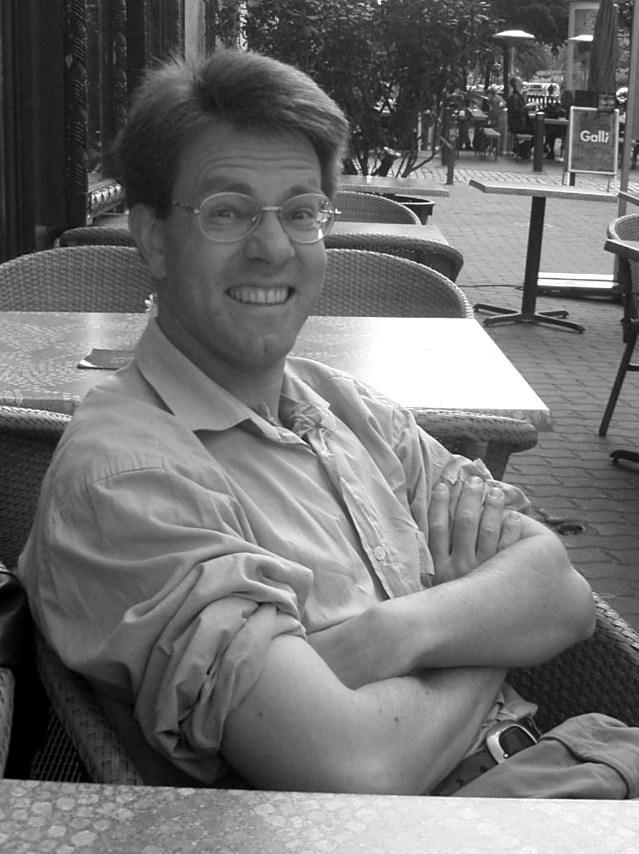
\includegraphics[width=0.33\textwidth]{claus_bernet_bw}
\end{floatingfigure}

Claus Bernet studierte Geschichtswissenschaften, Kunstgeschichte und
Stadtplanung in Berlin, Wien und Birmingham (UK). Die Dissertation erfolgte 2005
an der Martin-Luther-Universität Halle im Bereich Frühe Neuzeit.

\medskip

Parallel studierte er Erziehungswissenschaften an der Freien Universität Berlin.
2007 promovierte er mit einer Arbeit zur Erziehungsgedanken in nichtstaatlichen
Einrichtungen.

\medskip

Beschäftigung zu Themen der Gewaltprävention (PAG) und zur neosokratischen
Gesprächsführung; 2002/03 Mitarbeit beim Zentrum für Demokratische Kultur in
Berlin. 2008/09 koordinierte Bernet des Interview-Projektes "`Erweckte
Geschichte"'.

\medskip

Derzeit Arbeit er an einer Studie zu deutsch-italienischen Intellektuellen um
1900 mit einem Stipendiat des Literaturarchivs Marbach 2008. Desweiteren ist er
seid Jahren tätig als Mitarbeiter für die Lebenshilfe e.V. in Berlin.

\medskip

Die Forschungsgebiete von Claus Bernet sind historische Friedenskirchen,
Pietismus, Stadtgeschichte und Genossenschaftswesen.

\medskip

Folgende Veröffentlichungen zur Quäkerforschung sind bisher von Bernet
erschienen:

\begin{itemize}
 \item Rufus Jones (1863-1948). Life and Bibliography of an American Scholar,
Writer, and Social Activist. With a Foreword by Douglas Gwyn, New York 2009.
 \item Quäker aus Politik, Kunst und Wissenschaft in Deutschland. 20.
Jahrhundert. Ein biographisches Lexikon, Nordhausen 2007. 2. Auflage Nordhausen
2008. 3. Auflage in Planung.
 \item Between Quietism and Radical Pietism: The German Quaker Settlement
Friedensthal. 1792-1814, Birmingham 2004 (Woodbrooke Journal Series, 14).
\end{itemize}

\medskip


Claus Bernet ist Herausgeber der Reihe \textit{"`Deutsche Quäkerschriften"'}. Er
hält Vorträge in Deutschland, UK und USA zu Themen der Geschichte und Theologie
der Quäker. Ist Mitglied im Board of Trustees der englischen
Weiterbildungseinrichtung Woodbrooke in Birmingham seit 2004. Zahlreiche
Beiträge von ihm sind in der Zeitschrift "`Quäker"' -- dem Organ der Deutschen
Jahresversammlung e.V. -- erschienen.

\medskip

\begin{center}
\parbox{7,5cm}{
Tauroggener Str.2
\\10589 Berlin
\\bernet2@web.de
}
\end{center}

\pagebreak 
\vspace{\fill}

\fbox{
\parbox{9cm}{
\addcontentsline{toc}{chapter}{Impressum}
\textbf{Impressum:}\\
\medskip

Herausgeber:\\
\copyright{} Olaf Radicke, \copyright{} Claus Bernet\\
Alle Rechte vorbehalten\\
\medskip

München, \today \\
Version 1.0 \\
\medskip

Herstellung und Verlag:\\
Books on Demand GmbH, Norderstedt\\


ISBN: 978-3-8391-2608-0
}}
\pagebreak 

\end{document}

